\documentclass[twoside]{book}

% Packages required by doxygen
\usepackage{fixltx2e}
\usepackage{calc}
\usepackage{doxygen}
\usepackage[export]{adjustbox} % also loads graphicx
\usepackage{graphicx}
\usepackage[utf8]{inputenc}
\usepackage{makeidx}
\usepackage{multicol}
\usepackage{multirow}
\PassOptionsToPackage{warn}{textcomp}
\usepackage{textcomp}
\usepackage[nointegrals]{wasysym}
\usepackage[table]{xcolor}

% Font selection
\usepackage[T1]{fontenc}
\usepackage[scaled=.90]{helvet}
\usepackage{courier}
\usepackage{amssymb}
\usepackage{sectsty}
\renewcommand{\familydefault}{\sfdefault}
\allsectionsfont{%
  \fontseries{bc}\selectfont%
  \color{darkgray}%
}
\renewcommand{\DoxyLabelFont}{%
  \fontseries{bc}\selectfont%
  \color{darkgray}%
}
\newcommand{\+}{\discretionary{\mbox{\scriptsize$\hookleftarrow$}}{}{}}

% Page & text layout
\usepackage{geometry}
\geometry{%
  a4paper,%
  top=2.5cm,%
  bottom=2.5cm,%
  left=2.5cm,%
  right=2.5cm%
}
\tolerance=750
\hfuzz=15pt
\hbadness=750
\setlength{\emergencystretch}{15pt}
\setlength{\parindent}{0cm}
\setlength{\parskip}{3ex plus 2ex minus 2ex}
\makeatletter
\renewcommand{\paragraph}{%
  \@startsection{paragraph}{4}{0ex}{-1.0ex}{1.0ex}{%
    \normalfont\normalsize\bfseries\SS@parafont%
  }%
}
\renewcommand{\subparagraph}{%
  \@startsection{subparagraph}{5}{0ex}{-1.0ex}{1.0ex}{%
    \normalfont\normalsize\bfseries\SS@subparafont%
  }%
}
\makeatother

% Headers & footers
\usepackage{fancyhdr}
\pagestyle{fancyplain}
\fancyhead[LE]{\fancyplain{}{\bfseries\thepage}}
\fancyhead[CE]{\fancyplain{}{}}
\fancyhead[RE]{\fancyplain{}{\bfseries\leftmark}}
\fancyhead[LO]{\fancyplain{}{\bfseries\rightmark}}
\fancyhead[CO]{\fancyplain{}{}}
\fancyhead[RO]{\fancyplain{}{\bfseries\thepage}}
\fancyfoot[LE]{\fancyplain{}{}}
\fancyfoot[CE]{\fancyplain{}{}}
\fancyfoot[RE]{\fancyplain{}{\bfseries\scriptsize Generated by Doxygen }}
\fancyfoot[LO]{\fancyplain{}{\bfseries\scriptsize Generated by Doxygen }}
\fancyfoot[CO]{\fancyplain{}{}}
\fancyfoot[RO]{\fancyplain{}{}}
\renewcommand{\footrulewidth}{0.4pt}
\renewcommand{\chaptermark}[1]{%
  \markboth{#1}{}%
}
\renewcommand{\sectionmark}[1]{%
  \markright{\thesection\ #1}%
}

% Indices & bibliography
\usepackage{natbib}
\usepackage[titles]{tocloft}
\setcounter{tocdepth}{3}
\setcounter{secnumdepth}{5}
\makeindex

% Hyperlinks (required, but should be loaded last)
\usepackage{ifpdf}
\ifpdf
  \usepackage[pdftex,pagebackref=true]{hyperref}
\else
  \usepackage[ps2pdf,pagebackref=true]{hyperref}
\fi
\hypersetup{%
  colorlinks=true,%
  linkcolor=blue,%
  citecolor=blue,%
  unicode%
}

% Custom commands
\newcommand{\clearemptydoublepage}{%
  \newpage{\pagestyle{empty}\cleardoublepage}%
}

\usepackage{caption}
\captionsetup{labelsep=space,justification=centering,font={bf},singlelinecheck=off,skip=4pt,position=top}

%===== C O N T E N T S =====

\begin{document}

% Titlepage & ToC
\hypersetup{pageanchor=false,
             bookmarksnumbered=true,
             pdfencoding=unicode
            }
\pagenumbering{roman}
\begin{titlepage}
\vspace*{7cm}
\begin{center}%
{\Large C\+V\+DI G\+UI }\\
\vspace*{1cm}
{\large Generated by Doxygen 1.8.11}\\
\end{center}
\end{titlepage}
\clearemptydoublepage
\tableofcontents
\clearemptydoublepage
\pagenumbering{arabic}
\hypersetup{pageanchor=true}

%--- Begin generated contents ---
\chapter{Namespace Index}
\section{Namespace List}
Here is a list of all documented namespaces with brief descriptions\+:\begin{DoxyCompactList}
\item\contentsline{section}{\hyperlink{namespacecvdi}{cvdi} \\*Connected vehicle de-\/identification routines }{\pageref{namespacecvdi}}{}
\item\contentsline{section}{\hyperlink{namespacecvdi__multi}{cvdi\+\_\+multi} \\*Multi-\/threaded connected vehicle command line tool }{\pageref{namespacecvdi__multi}}{}
\item\contentsline{section}{\hyperlink{namespacegeo}{geo} \\*Namespace for geospatial and geodesic tool functions }{\pageref{namespacegeo}}{}
\item\contentsline{section}{\hyperlink{namespacegeo__data}{geo\+\_\+data} \\*Routines and data structures for reading, writing, and displaying geospatial data }{\pageref{namespacegeo__data}}{}
\item\contentsline{section}{\hyperlink{namespacehmm__mm}{hmm\+\_\+mm} \\*Hidden Markov Model Map Matching }{\pageref{namespacehmm__mm}}{}
\item\contentsline{section}{\hyperlink{namespacetool}{tool} \\*Namespace for command line tool functions }{\pageref{namespacetool}}{}
\item\contentsline{section}{\hyperlink{namespaceutil}{util} \\*Namespace for utility functions }{\pageref{namespaceutil}}{}
\end{DoxyCompactList}

\chapter{Hierarchical Index}
\section{Class Hierarchy}
This inheritance list is sorted roughly, but not completely, alphabetically\+:\begin{DoxyCompactList}
\item Allocator\begin{DoxyCompactList}
\item \contentsline{section}{fmt\+:\+:internal\+:\+:Memory\+Buffer$<$ T, S\+I\+ZE, Allocator $>$}{\pageref{classfmt_1_1internal_1_1MemoryBuffer}}{}
\item \contentsline{section}{fmt\+:\+:internal\+:\+:Memory\+Buffer$<$ Char, internal\+:\+:I\+N\+L\+I\+N\+E\+\_\+\+B\+U\+F\+F\+E\+R\+\_\+\+S\+I\+ZE, Allocator $>$}{\pageref{classfmt_1_1internal_1_1MemoryBuffer}}{}
\end{DoxyCompactList}
\item \contentsline{section}{geo\+:\+:Area}{\pageref{classgeo_1_1Area}}{}
\item \contentsline{section}{cvdi\+:\+:Area\+Fitter}{\pageref{classcvdi_1_1AreaFitter}}{}
\item \contentsline{section}{fmt\+:\+:internal\+:\+:Arg\+Array$<$ N, bool $>$}{\pageref{structfmt_1_1internal_1_1ArgArray}}{}
\item \contentsline{section}{fmt\+:\+:internal\+:\+:Arg\+Array$<$ N, false $>$}{\pageref{structfmt_1_1internal_1_1ArgArray_3_01N_00_01false_01_4}}{}
\item \contentsline{section}{fmt\+:\+:internal\+:\+:Arg\+Array$<$ N, true $>$}{\pageref{structfmt_1_1internal_1_1ArgArray_3_01N_00_01true_01_4}}{}
\item \contentsline{section}{fmt\+:\+:Arg\+List}{\pageref{classfmt_1_1ArgList}}{}
\item \contentsline{section}{fmt\+:\+:internal\+:\+:Arg\+Map$<$ Char $>$}{\pageref{classfmt_1_1internal_1_1ArgMap}}{}
\item \contentsline{section}{fmt\+:\+:internal\+:\+:Arg\+Type}{\pageref{structfmt_1_1internal_1_1ArgType}}{}
\item \contentsline{section}{fmt\+:\+:Arg\+Visitor$<$ Impl, Result $>$}{\pageref{classfmt_1_1ArgVisitor}}{}
\item \contentsline{section}{fmt\+:\+:Arg\+Visitor$<$ Arg\+Formatter$<$ Char $>$, void $>$}{\pageref{classfmt_1_1ArgVisitor}}{}
\begin{DoxyCompactList}
\item \contentsline{section}{fmt\+:\+:internal\+:\+:Arg\+Formatter\+Base$<$ Arg\+Formatter$<$ Char $>$, Char $>$}{\pageref{classfmt_1_1internal_1_1ArgFormatterBase}}{}
\begin{DoxyCompactList}
\item \contentsline{section}{fmt\+:\+:Basic\+Arg\+Formatter$<$ Arg\+Formatter$<$ Char $>$, Char $>$}{\pageref{classfmt_1_1BasicArgFormatter}}{}
\begin{DoxyCompactList}
\item \contentsline{section}{fmt\+:\+:Arg\+Formatter$<$ Char $>$}{\pageref{classfmt_1_1ArgFormatter}}{}
\end{DoxyCompactList}
\end{DoxyCompactList}
\end{DoxyCompactList}
\item \contentsline{section}{fmt\+:\+:Arg\+Visitor$<$ Impl, void $>$}{\pageref{classfmt_1_1ArgVisitor}}{}
\begin{DoxyCompactList}
\item \contentsline{section}{fmt\+:\+:internal\+:\+:Arg\+Formatter\+Base$<$ Impl, Char $>$}{\pageref{classfmt_1_1internal_1_1ArgFormatterBase}}{}
\begin{DoxyCompactList}
\item \contentsline{section}{fmt\+:\+:Basic\+Arg\+Formatter$<$ Impl, Char $>$}{\pageref{classfmt_1_1BasicArgFormatter}}{}
\end{DoxyCompactList}
\end{DoxyCompactList}
\item \contentsline{section}{fmt\+:\+:Arg\+Visitor$<$ Printf\+Arg\+Formatter$<$ Char $>$, void $>$}{\pageref{classfmt_1_1ArgVisitor}}{}
\begin{DoxyCompactList}
\item \contentsline{section}{fmt\+:\+:internal\+:\+:Arg\+Formatter\+Base$<$ Printf\+Arg\+Formatter$<$ Char $>$, Char $>$}{\pageref{classfmt_1_1internal_1_1ArgFormatterBase}}{}
\begin{DoxyCompactList}
\item \contentsline{section}{fmt\+:\+:internal\+:\+:Printf\+Arg\+Formatter$<$ Char $>$}{\pageref{classfmt_1_1internal_1_1PrintfArgFormatter}}{}
\end{DoxyCompactList}
\end{DoxyCompactList}
\item \contentsline{section}{spdlog\+:\+:details\+:\+:async\+\_\+log\+\_\+helper}{\pageref{classspdlog_1_1details_1_1async__log__helper}}{}
\item basic\+\_\+streambuf\begin{DoxyCompactList}
\item \contentsline{section}{fmt\+:\+:internal\+:\+:Format\+Buf$<$ Char $>$}{\pageref{classfmt_1_1internal_1_1FormatBuf}}{}
\end{DoxyCompactList}
\item \contentsline{section}{fmt\+:\+:internal\+:\+:Basic\+Char\+Traits$<$ Char $>$}{\pageref{classfmt_1_1internal_1_1BasicCharTraits}}{}
\item \contentsline{section}{fmt\+:\+:internal\+:\+:Basic\+Char\+Traits$<$ char $>$}{\pageref{classfmt_1_1internal_1_1BasicCharTraits}}{}
\begin{DoxyCompactList}
\item \contentsline{section}{fmt\+:\+:internal\+:\+:Char\+Traits$<$ char $>$}{\pageref{classfmt_1_1internal_1_1CharTraits_3_01char_01_4}}{}
\end{DoxyCompactList}
\item \contentsline{section}{fmt\+:\+:internal\+:\+:Basic\+Char\+Traits$<$ wchar\+\_\+t $>$}{\pageref{classfmt_1_1internal_1_1BasicCharTraits}}{}
\begin{DoxyCompactList}
\item \contentsline{section}{fmt\+:\+:internal\+:\+:Char\+Traits$<$ wchar\+\_\+t $>$}{\pageref{classfmt_1_1internal_1_1CharTraits_3_01wchar__t_01_4}}{}
\end{DoxyCompactList}
\item \contentsline{section}{fmt\+:\+:Basic\+C\+String\+Ref$<$ Char $>$}{\pageref{classfmt_1_1BasicCStringRef}}{}
\item \contentsline{section}{fmt\+:\+:internal\+:\+:Basic\+Data$<$ T $>$}{\pageref{structfmt_1_1internal_1_1BasicData}}{}
\item \contentsline{section}{fmt\+:\+:Basic\+String\+Ref$<$ Char $>$}{\pageref{classfmt_1_1BasicStringRef}}{}
\item \contentsline{section}{fmt\+:\+:Basic\+String\+Ref$<$ char $>$}{\pageref{classfmt_1_1BasicStringRef}}{}
\item \contentsline{section}{fmt\+:\+:Basic\+Writer$<$ Char $>$}{\pageref{classfmt_1_1BasicWriter}}{}
\begin{DoxyCompactList}
\item \contentsline{section}{fmt\+:\+:Basic\+Array\+Writer$<$ Char $>$}{\pageref{classfmt_1_1BasicArrayWriter}}{}
\item \contentsline{section}{fmt\+:\+:Basic\+Memory\+Writer$<$ Char, Allocator $>$}{\pageref{classfmt_1_1BasicMemoryWriter}}{}
\end{DoxyCompactList}
\item \contentsline{section}{fmt\+:\+:Buffer$<$ T $>$}{\pageref{classfmt_1_1Buffer}}{}
\begin{DoxyCompactList}
\item \contentsline{section}{fmt\+:\+:internal\+:\+:Memory\+Buffer$<$ T, S\+I\+ZE, Allocator $>$}{\pageref{classfmt_1_1internal_1_1MemoryBuffer}}{}
\end{DoxyCompactList}
\item \contentsline{section}{fmt\+:\+:Buffer$<$ Char $>$}{\pageref{classfmt_1_1Buffer}}{}
\begin{DoxyCompactList}
\item \contentsline{section}{fmt\+:\+:internal\+:\+:Fixed\+Buffer$<$ Char $>$}{\pageref{classfmt_1_1internal_1_1FixedBuffer}}{}
\item \contentsline{section}{fmt\+:\+:internal\+:\+:Memory\+Buffer$<$ Char, internal\+:\+:I\+N\+L\+I\+N\+E\+\_\+\+B\+U\+F\+F\+E\+R\+\_\+\+S\+I\+ZE, Allocator $>$}{\pageref{classfmt_1_1internal_1_1MemoryBuffer}}{}
\end{DoxyCompactList}
\item \contentsline{section}{fmt\+:\+:Buffered\+File}{\pageref{classfmt_1_1BufferedFile}}{}
\item \contentsline{section}{fmt\+:\+:internal\+:\+:Char\+Traits$<$ Char $>$}{\pageref{classfmt_1_1internal_1_1CharTraits}}{}
\item \contentsline{section}{fmt\+:\+:internal\+:\+:Conditional$<$ B, T, F $>$}{\pageref{structfmt_1_1internal_1_1Conditional}}{}
\item \contentsline{section}{fmt\+:\+:internal\+:\+:Conditional$<$ false, T, F $>$}{\pageref{structfmt_1_1internal_1_1Conditional_3_01false_00_01T_00_01F_01_4}}{}
\item \contentsline{section}{config\+:\+:Config}{\pageref{classconfig_1_1Config}}{}
\item \contentsline{section}{fmt\+:\+:internal\+:\+:Convert\+To\+Int$<$ T $>$}{\pageref{structfmt_1_1internal_1_1ConvertToInt}}{}
\item \contentsline{section}{fmt\+:\+:internal\+:\+:Convert\+To\+Int\+Impl$<$ T, E\+N\+A\+B\+L\+E\+\_\+\+C\+O\+N\+V\+E\+R\+S\+I\+ON $>$}{\pageref{structfmt_1_1internal_1_1ConvertToIntImpl}}{}
\item \contentsline{section}{fmt\+:\+:internal\+:\+:Convert\+To\+Int\+Impl2$<$ T, E\+N\+A\+B\+L\+E\+\_\+\+C\+O\+N\+V\+E\+R\+S\+I\+ON $>$}{\pageref{structfmt_1_1internal_1_1ConvertToIntImpl2}}{}
\item \contentsline{section}{fmt\+:\+:internal\+:\+:Convert\+To\+Int\+Impl2$<$ T, true $>$}{\pageref{structfmt_1_1internal_1_1ConvertToIntImpl2_3_01T_00_01true_01_4}}{}
\item \contentsline{section}{fmt\+:\+:internal\+:\+:Convert\+To\+Int\+Impl$<$ T, true $>$}{\pageref{structfmt_1_1internal_1_1ConvertToIntImpl_3_01T_00_01true_01_4}}{}
\item \contentsline{section}{geo\+\_\+data\+:\+:C\+S\+V\+Road\+Writer}{\pageref{classgeo__data_1_1CSVRoadWriter}}{}
\item \contentsline{section}{fmt\+:\+:internal\+:\+:Value\+:\+:Custom\+Value}{\pageref{structfmt_1_1internal_1_1Value_1_1CustomValue}}{}
\item \contentsline{section}{spdlog\+:\+:sinks\+:\+:dateonly\+\_\+daily\+\_\+file\+\_\+name\+\_\+calculator}{\pageref{structspdlog_1_1sinks_1_1dateonly__daily__file__name__calculator}}{}
\item \contentsline{section}{spdlog\+:\+:sinks\+:\+:default\+\_\+daily\+\_\+file\+\_\+name\+\_\+calculator}{\pageref{structspdlog_1_1sinks_1_1default__daily__file__name__calculator}}{}
\item \contentsline{section}{cvdi\+:\+:Stop\+:\+:Deque}{\pageref{classcvdi_1_1Stop_1_1Deque}}{}
\item \contentsline{section}{fmt\+:\+:internal\+:\+:Dummy\+Int}{\pageref{structfmt_1_1internal_1_1DummyInt}}{}
\item \contentsline{section}{geo\+:\+:Edge}{\pageref{classgeo_1_1Edge}}{}
\item \contentsline{section}{hmm\+\_\+mm\+:\+:Emission\+State}{\pageref{classhmm__mm_1_1EmissionState}}{}
\item \contentsline{section}{fmt\+:\+:Empty\+Spec}{\pageref{structfmt_1_1EmptySpec}}{}
\begin{DoxyCompactList}
\item \contentsline{section}{fmt\+:\+:Type\+Spec$<$ T\+Y\+PE $>$}{\pageref{structfmt_1_1TypeSpec}}{}
\end{DoxyCompactList}
\item \contentsline{section}{fmt\+:\+:internal\+:\+:Enable\+If$<$ B, T $>$}{\pageref{structfmt_1_1internal_1_1EnableIf}}{}
\item \contentsline{section}{fmt\+:\+:internal\+:\+:Enable\+If$<$ true, T $>$}{\pageref{structfmt_1_1internal_1_1EnableIf_3_01true_00_01T_01_4}}{}
\item \contentsline{section}{fmt\+:\+:Error\+Code}{\pageref{classfmt_1_1ErrorCode}}{}
\item exception\begin{DoxyCompactList}
\item \contentsline{section}{spdlog\+:\+:spdlog\+\_\+ex}{\pageref{classspdlog_1_1spdlog__ex}}{}
\end{DoxyCompactList}
\item \contentsline{section}{fmt\+:\+:File}{\pageref{classfmt_1_1File}}{}
\item \contentsline{section}{spdlog\+:\+:details\+:\+:file\+\_\+helper}{\pageref{classspdlog_1_1details_1_1file__helper}}{}
\item \contentsline{section}{cvdi\+\_\+multi\+:\+:File\+Info}{\pageref{classcvdi__multi_1_1FileInfo}}{}
\begin{DoxyCompactList}
\item \contentsline{section}{cvdi\+\_\+multi\+:\+:Single\+File\+Info}{\pageref{classcvdi__multi_1_1SingleFileInfo}}{}
\end{DoxyCompactList}
\item \contentsline{section}{spdlog\+:\+:details\+:\+:flag\+\_\+formatter}{\pageref{classspdlog_1_1details_1_1flag__formatter}}{}
\begin{DoxyCompactList}
\item \contentsline{section}{spdlog\+:\+:details\+:\+:a\+\_\+formatter}{\pageref{classspdlog_1_1details_1_1a__formatter}}{}
\item \contentsline{section}{spdlog\+:\+:details\+:\+:b\+\_\+formatter}{\pageref{classspdlog_1_1details_1_1b__formatter}}{}
\item \contentsline{section}{spdlog\+:\+:details\+:\+:level\+\_\+formatter}{\pageref{classspdlog_1_1details_1_1level__formatter}}{}
\item \contentsline{section}{spdlog\+:\+:details\+:\+:short\+\_\+level\+\_\+formatter}{\pageref{classspdlog_1_1details_1_1short__level__formatter}}{}
\item \contentsline{section}{spdlog\+:\+:details\+:\+:S\+P\+D\+L\+O\+G\+\_\+\+F\+I\+N\+AL}{\pageref{classspdlog_1_1details_1_1SPDLOG__FINAL}}{}
\item \contentsline{section}{spdlog\+:\+:details\+:\+:S\+P\+D\+L\+O\+G\+\_\+\+F\+I\+N\+AL}{\pageref{classspdlog_1_1details_1_1SPDLOG__FINAL}}{}
\item \contentsline{section}{spdlog\+:\+:details\+:\+:S\+P\+D\+L\+O\+G\+\_\+\+F\+I\+N\+AL}{\pageref{classspdlog_1_1details_1_1SPDLOG__FINAL}}{}
\item \contentsline{section}{spdlog\+:\+:details\+:\+:S\+P\+D\+L\+O\+G\+\_\+\+F\+I\+N\+AL}{\pageref{classspdlog_1_1details_1_1SPDLOG__FINAL}}{}
\item \contentsline{section}{spdlog\+:\+:details\+:\+:S\+P\+D\+L\+O\+G\+\_\+\+F\+I\+N\+AL}{\pageref{classspdlog_1_1details_1_1SPDLOG__FINAL}}{}
\item \contentsline{section}{spdlog\+:\+:details\+:\+:S\+P\+D\+L\+O\+G\+\_\+\+F\+I\+N\+AL}{\pageref{classspdlog_1_1details_1_1SPDLOG__FINAL}}{}
\item \contentsline{section}{spdlog\+:\+:details\+:\+:S\+P\+D\+L\+O\+G\+\_\+\+F\+I\+N\+AL}{\pageref{classspdlog_1_1details_1_1SPDLOG__FINAL}}{}
\item \contentsline{section}{spdlog\+:\+:details\+:\+:S\+P\+D\+L\+O\+G\+\_\+\+F\+I\+N\+AL}{\pageref{classspdlog_1_1details_1_1SPDLOG__FINAL}}{}
\item \contentsline{section}{spdlog\+:\+:details\+:\+:S\+P\+D\+L\+O\+G\+\_\+\+F\+I\+N\+AL}{\pageref{classspdlog_1_1details_1_1SPDLOG__FINAL}}{}
\item \contentsline{section}{spdlog\+:\+:details\+:\+:S\+P\+D\+L\+O\+G\+\_\+\+F\+I\+N\+AL}{\pageref{classspdlog_1_1details_1_1SPDLOG__FINAL}}{}
\item \contentsline{section}{spdlog\+:\+:details\+:\+:S\+P\+D\+L\+O\+G\+\_\+\+F\+I\+N\+AL}{\pageref{classspdlog_1_1details_1_1SPDLOG__FINAL}}{}
\item \contentsline{section}{spdlog\+:\+:details\+:\+:S\+P\+D\+L\+O\+G\+\_\+\+F\+I\+N\+AL}{\pageref{classspdlog_1_1details_1_1SPDLOG__FINAL}}{}
\item \contentsline{section}{spdlog\+:\+:details\+:\+:S\+P\+D\+L\+O\+G\+\_\+\+F\+I\+N\+AL}{\pageref{classspdlog_1_1details_1_1SPDLOG__FINAL}}{}
\item \contentsline{section}{spdlog\+:\+:details\+:\+:S\+P\+D\+L\+O\+G\+\_\+\+F\+I\+N\+AL}{\pageref{classspdlog_1_1details_1_1SPDLOG__FINAL}}{}
\item \contentsline{section}{spdlog\+:\+:details\+:\+:S\+P\+D\+L\+O\+G\+\_\+\+F\+I\+N\+AL}{\pageref{classspdlog_1_1details_1_1SPDLOG__FINAL}}{}
\item \contentsline{section}{spdlog\+:\+:details\+:\+:S\+P\+D\+L\+O\+G\+\_\+\+F\+I\+N\+AL}{\pageref{classspdlog_1_1details_1_1SPDLOG__FINAL}}{}
\item \contentsline{section}{spdlog\+:\+:details\+:\+:S\+P\+D\+L\+O\+G\+\_\+\+F\+I\+N\+AL}{\pageref{classspdlog_1_1details_1_1SPDLOG__FINAL}}{}
\item \contentsline{section}{spdlog\+:\+:details\+:\+:S\+P\+D\+L\+O\+G\+\_\+\+F\+I\+N\+AL}{\pageref{classspdlog_1_1details_1_1SPDLOG__FINAL}}{}
\item \contentsline{section}{spdlog\+:\+:details\+:\+:S\+P\+D\+L\+O\+G\+\_\+\+F\+I\+N\+AL}{\pageref{classspdlog_1_1details_1_1SPDLOG__FINAL}}{}
\item \contentsline{section}{spdlog\+:\+:details\+:\+:S\+P\+D\+L\+O\+G\+\_\+\+F\+I\+N\+AL}{\pageref{classspdlog_1_1details_1_1SPDLOG__FINAL}}{}
\item \contentsline{section}{spdlog\+:\+:details\+:\+:S\+P\+D\+L\+O\+G\+\_\+\+F\+I\+N\+AL}{\pageref{classspdlog_1_1details_1_1SPDLOG__FINAL}}{}
\item \contentsline{section}{spdlog\+:\+:details\+:\+:S\+P\+D\+L\+O\+G\+\_\+\+F\+I\+N\+AL}{\pageref{classspdlog_1_1details_1_1SPDLOG__FINAL}}{}
\item \contentsline{section}{spdlog\+:\+:details\+:\+:S\+P\+D\+L\+O\+G\+\_\+\+F\+I\+N\+AL}{\pageref{classspdlog_1_1details_1_1SPDLOG__FINAL}}{}
\item \contentsline{section}{spdlog\+:\+:details\+:\+:S\+P\+D\+L\+O\+G\+\_\+\+F\+I\+N\+AL}{\pageref{classspdlog_1_1details_1_1SPDLOG__FINAL}}{}
\item \contentsline{section}{spdlog\+:\+:details\+:\+:S\+P\+D\+L\+O\+G\+\_\+\+F\+I\+N\+AL}{\pageref{classspdlog_1_1details_1_1SPDLOG__FINAL}}{}
\item \contentsline{section}{spdlog\+:\+:details\+:\+:S\+P\+D\+L\+O\+G\+\_\+\+F\+I\+N\+AL}{\pageref{classspdlog_1_1details_1_1SPDLOG__FINAL}}{}
\item \contentsline{section}{spdlog\+:\+:details\+:\+:S\+P\+D\+L\+O\+G\+\_\+\+F\+I\+N\+AL}{\pageref{classspdlog_1_1details_1_1SPDLOG__FINAL}}{}
\end{DoxyCompactList}
\item \contentsline{section}{fmt\+:\+:Format\+Int}{\pageref{classfmt_1_1FormatInt}}{}
\item \contentsline{section}{spdlog\+:\+:formatter}{\pageref{classspdlog_1_1formatter}}{}
\begin{DoxyCompactList}
\item \contentsline{section}{spdlog\+:\+:S\+P\+D\+L\+O\+G\+\_\+\+F\+I\+N\+AL}{\pageref{classspdlog_1_1SPDLOG__FINAL}}{}
\end{DoxyCompactList}
\item \contentsline{section}{fmt\+:\+:internal\+:\+:Formatter\+Base}{\pageref{classfmt_1_1internal_1_1FormatterBase}}{}
\begin{DoxyCompactList}
\item \contentsline{section}{fmt\+:\+:Basic\+Formatter$<$ Char, Arg\+Formatter$<$ Char $>$ $>$}{\pageref{classfmt_1_1BasicFormatter}}{}
\item \contentsline{section}{fmt\+:\+:Basic\+Formatter$<$ Char, Impl $>$}{\pageref{classfmt_1_1BasicFormatter}}{}
\item \contentsline{section}{fmt\+:\+:Basic\+Formatter$<$ Char\+Type, Arg\+Formatter $>$}{\pageref{classfmt_1_1BasicFormatter}}{}
\item \contentsline{section}{fmt\+:\+:internal\+:\+:Printf\+Formatter$<$ Char $>$}{\pageref{classfmt_1_1internal_1_1PrintfFormatter}}{}
\end{DoxyCompactList}
\item \contentsline{section}{cvdi\+:\+:Intersection\+Counter}{\pageref{classcvdi_1_1IntersectionCounter}}{}
\item \contentsline{section}{geo\+\_\+data\+:\+:Interval}{\pageref{classgeo__data_1_1Interval}}{}
\item \contentsline{section}{geo\+\_\+data\+:\+:Interval\+Marker}{\pageref{classgeo__data_1_1IntervalMarker}}{}
\item \contentsline{section}{fmt\+:\+:internal\+:\+:Int\+Traits$<$ T $>$}{\pageref{structfmt_1_1internal_1_1IntTraits}}{}
\item \contentsline{section}{geo\+\_\+data\+:\+:K\+ML}{\pageref{classgeo__data_1_1KML}}{}
\item \contentsline{section}{fmt\+:\+:internal\+:\+:L\+Conv\+Check$<$ T, T $>$}{\pageref{structfmt_1_1internal_1_1LConvCheck}}{}
\item \contentsline{section}{spdlog\+:\+:details\+:\+:log\+\_\+msg}{\pageref{structspdlog_1_1details_1_1log__msg}}{}
\item \contentsline{section}{spdlog\+:\+:logger}{\pageref{classspdlog_1_1logger}}{}
\begin{DoxyCompactList}
\item \contentsline{section}{spdlog\+:\+:S\+P\+D\+L\+O\+G\+\_\+\+F\+I\+N\+AL}{\pageref{classspdlog_1_1SPDLOG__FINAL}}{}
\end{DoxyCompactList}
\item \contentsline{section}{fmt\+:\+:internal\+:\+:Make\+Unsigned$<$ T $>$}{\pageref{structfmt_1_1internal_1_1MakeUnsigned}}{}
\item \contentsline{section}{hmm\+\_\+mm\+:\+:Mark}{\pageref{classhmm__mm_1_1Mark}}{}
\item \contentsline{section}{hmm\+\_\+mm\+:\+:Mark\+Comparison}{\pageref{classhmm__mm_1_1MarkComparison}}{}
\item \contentsline{section}{hmm\+\_\+mm\+:\+:Matcher}{\pageref{classhmm__mm_1_1Matcher}}{}
\item \contentsline{section}{spdlog\+:\+:details\+:\+:mpmc\+\_\+bounded\+\_\+queue$<$ T $>$}{\pageref{classspdlog_1_1details_1_1mpmc__bounded__queue}}{}
\item \contentsline{section}{spdlog\+:\+:details\+:\+:mpmc\+\_\+bounded\+\_\+queue$<$ item\+\_\+type $>$}{\pageref{classspdlog_1_1details_1_1mpmc__bounded__queue}}{}
\item \contentsline{section}{fmt\+:\+:internal\+:\+:Not$<$ bool $>$}{\pageref{structfmt_1_1internal_1_1Not}}{}
\item \contentsline{section}{fmt\+:\+:internal\+:\+:Not$<$ false $>$}{\pageref{structfmt_1_1internal_1_1Not_3_01false_01_4}}{}
\item \contentsline{section}{fmt\+:\+:internal\+:\+:No\+Thousands\+Sep}{\pageref{structfmt_1_1internal_1_1NoThousandsSep}}{}
\item \contentsline{section}{fmt\+:\+:internal\+:\+:Null$<$ T $>$}{\pageref{structfmt_1_1internal_1_1Null}}{}
\item \contentsline{section}{spdlog\+:\+:details\+:\+:null\+\_\+atomic\+\_\+int}{\pageref{structspdlog_1_1details_1_1null__atomic__int}}{}
\item \contentsline{section}{spdlog\+:\+:details\+:\+:null\+\_\+mutex}{\pageref{structspdlog_1_1details_1_1null__mutex}}{}
\item numeric\+\_\+limits\begin{DoxyCompactList}
\item \contentsline{section}{std\+:\+:numeric\+\_\+limits$<$ fmt\+:\+:internal\+:\+:Dummy\+Int $>$}{\pageref{classstd_1_1numeric__limits_3_01fmt_1_1internal_1_1DummyInt_01_4}}{}
\end{DoxyCompactList}
\item \contentsline{section}{tool\+:\+:Option}{\pageref{classtool_1_1Option}}{}
\item ostream\begin{DoxyCompactList}
\item \contentsline{section}{fmt\+:\+:internal\+:\+:Dummy\+Stream}{\pageref{structfmt_1_1internal_1_1DummyStream}}{}
\end{DoxyCompactList}
\item \contentsline{section}{Multi\+Thread\+:\+:Parallel$<$ T $>$}{\pageref{classMultiThread_1_1Parallel}}{}
\item \contentsline{section}{Multi\+Thread\+:\+:Parallel$<$ File\+Info $>$}{\pageref{classMultiThread_1_1Parallel}}{}
\begin{DoxyCompactList}
\item \contentsline{section}{cvdi\+\_\+multi\+:\+:Batch\+Parallel}{\pageref{classcvdi__multi_1_1BatchParallel}}{}
\begin{DoxyCompactList}
\item \contentsline{section}{cvdi\+\_\+multi\+:\+:Single\+Batch\+Parallel}{\pageref{classcvdi__multi_1_1SingleBatchParallel}}{}
\begin{DoxyCompactList}
\item \contentsline{section}{cvdi\+\_\+multi\+:\+:C\+V\+D\+I\+Parallel}{\pageref{classcvdi__multi_1_1CVDIParallel}}{}
\end{DoxyCompactList}
\end{DoxyCompactList}
\end{DoxyCompactList}
\item \contentsline{section}{cvdi\+:\+:Point\+Counter}{\pageref{structcvdi_1_1PointCounter}}{}
\item \contentsline{section}{cvdi\+:\+:Privacy\+Interval\+Finder}{\pageref{classcvdi_1_1PrivacyIntervalFinder}}{}
\item \contentsline{section}{spdlog\+:\+:details\+:\+:registry\+\_\+t$<$ Mutex $>$}{\pageref{classspdlog_1_1details_1_1registry__t}}{}
\item \contentsline{section}{geo\+:\+:Road}{\pageref{classgeo_1_1Road}}{}
\item \contentsline{section}{hmm\+\_\+mm\+:\+:Road\+Map}{\pageref{classhmm__mm_1_1RoadMap}}{}
\item \contentsline{section}{hmm\+\_\+mm\+:\+:Road\+Point}{\pageref{classhmm__mm_1_1RoadPoint}}{}
\item \contentsline{section}{geo\+\_\+data\+:\+:Road\+Reader}{\pageref{classgeo__data_1_1RoadReader}}{}
\begin{DoxyCompactList}
\item \contentsline{section}{geo\+\_\+data\+:\+:C\+S\+V\+Road\+Reader}{\pageref{classgeo__data_1_1CSVRoadReader}}{}
\item \contentsline{section}{geo\+\_\+data\+:\+:Post\+G\+I\+S\+Road\+Reader}{\pageref{classgeo__data_1_1PostGISRoadReader}}{}
\end{DoxyCompactList}
\item \contentsline{section}{hmm\+\_\+mm\+:\+:Router}{\pageref{classhmm__mm_1_1Router}}{}
\item runtime\+\_\+error\begin{DoxyCompactList}
\item \contentsline{section}{fmt\+:\+:Format\+Error}{\pageref{classfmt_1_1FormatError}}{}
\item \contentsline{section}{fmt\+:\+:internal\+:\+:Runtime\+Error}{\pageref{classfmt_1_1internal_1_1RuntimeError}}{}
\begin{DoxyCompactList}
\item \contentsline{section}{fmt\+:\+:System\+Error}{\pageref{classfmt_1_1SystemError}}{}
\end{DoxyCompactList}
\end{DoxyCompactList}
\item \contentsline{section}{geo\+\_\+data\+:\+:Sample}{\pageref{classgeo__data_1_1Sample}}{}
\item \contentsline{section}{Multi\+Thread\+:\+:Shared\+Queue$<$ T $>$}{\pageref{classMultiThread_1_1SharedQueue}}{}
\item \contentsline{section}{fmt\+:\+:internal\+:\+:Sign\+Checker$<$ Is\+Signed $>$}{\pageref{structfmt_1_1internal_1_1SignChecker}}{}
\item \contentsline{section}{fmt\+:\+:internal\+:\+:Sign\+Checker$<$ false $>$}{\pageref{structfmt_1_1internal_1_1SignChecker_3_01false_01_4}}{}
\item \contentsline{section}{spdlog\+:\+:sinks\+:\+:sink}{\pageref{classspdlog_1_1sinks_1_1sink}}{}
\begin{DoxyCompactList}
\item \contentsline{section}{spdlog\+:\+:sinks\+:\+:base\+\_\+sink$<$ Mutex $>$}{\pageref{classspdlog_1_1sinks_1_1base__sink}}{}
\begin{DoxyCompactList}
\item \contentsline{section}{spdlog\+:\+:sinks\+:\+:ansicolor\+\_\+sink$<$ Mutex $>$}{\pageref{classspdlog_1_1sinks_1_1ansicolor__sink}}{}
\begin{DoxyCompactList}
\item \contentsline{section}{spdlog\+:\+:sinks\+:\+:ansicolor\+\_\+stderr\+\_\+sink$<$ Mutex $>$}{\pageref{classspdlog_1_1sinks_1_1ansicolor__stderr__sink}}{}
\item \contentsline{section}{spdlog\+:\+:sinks\+:\+:ansicolor\+\_\+stdout\+\_\+sink$<$ Mutex $>$}{\pageref{classspdlog_1_1sinks_1_1ansicolor__stdout__sink}}{}
\end{DoxyCompactList}
\item \contentsline{section}{spdlog\+:\+:sinks\+:\+:dist\+\_\+sink$<$ Mutex $>$}{\pageref{classspdlog_1_1sinks_1_1dist__sink}}{}
\item \contentsline{section}{spdlog\+:\+:sinks\+:\+:null\+\_\+sink$<$ Mutex $>$}{\pageref{classspdlog_1_1sinks_1_1null__sink}}{}
\item \contentsline{section}{spdlog\+:\+:sinks\+:\+:ostream\+\_\+sink$<$ Mutex $>$}{\pageref{classspdlog_1_1sinks_1_1ostream__sink}}{}
\item \contentsline{section}{spdlog\+:\+:sinks\+:\+:S\+P\+D\+L\+O\+G\+\_\+\+F\+I\+N\+AL$<$ Mutex $>$}{\pageref{classspdlog_1_1sinks_1_1SPDLOG__FINAL}}{}
\item \contentsline{section}{spdlog\+:\+:sinks\+:\+:S\+P\+D\+L\+O\+G\+\_\+\+F\+I\+N\+AL$<$ Mutex $>$}{\pageref{classspdlog_1_1sinks_1_1SPDLOG__FINAL}}{}
\item \contentsline{section}{spdlog\+:\+:sinks\+:\+:S\+P\+D\+L\+O\+G\+\_\+\+F\+I\+N\+AL$<$ Mutex $>$}{\pageref{classspdlog_1_1sinks_1_1SPDLOG__FINAL}}{}
\item \contentsline{section}{spdlog\+:\+:sinks\+:\+:S\+P\+D\+L\+O\+G\+\_\+\+F\+I\+N\+AL$<$ Mutex $>$}{\pageref{classspdlog_1_1sinks_1_1SPDLOG__FINAL}}{}
\item \contentsline{section}{spdlog\+:\+:sinks\+:\+:S\+P\+D\+L\+O\+G\+\_\+\+F\+I\+N\+AL$<$ Mutex $>$}{\pageref{classspdlog_1_1sinks_1_1SPDLOG__FINAL}}{}
\item \contentsline{section}{spdlog\+:\+:sinks\+:\+:wincolor\+\_\+sink$<$ Mutex $>$}{\pageref{classspdlog_1_1sinks_1_1wincolor__sink}}{}
\begin{DoxyCompactList}
\item \contentsline{section}{spdlog\+:\+:sinks\+:\+:wincolor\+\_\+stderr\+\_\+sink$<$ Mutex $>$}{\pageref{classspdlog_1_1sinks_1_1wincolor__stderr__sink}}{}
\item \contentsline{section}{spdlog\+:\+:sinks\+:\+:wincolor\+\_\+stdout\+\_\+sink$<$ Mutex $>$}{\pageref{classspdlog_1_1sinks_1_1wincolor__stdout__sink}}{}
\end{DoxyCompactList}
\end{DoxyCompactList}
\end{DoxyCompactList}
\item \contentsline{section}{geo\+:\+:Spatial}{\pageref{classgeo_1_1Spatial}}{}
\item SpecT\begin{DoxyCompactList}
\item \contentsline{section}{fmt\+:\+:Int\+Format\+Spec$<$ T, SpecT, Char $>$}{\pageref{classfmt_1_1IntFormatSpec}}{}
\end{DoxyCompactList}
\item \contentsline{section}{cvdi\+:\+:Start\+End\+Intervals}{\pageref{classcvdi_1_1StartEndIntervals}}{}
\item \contentsline{section}{cvdi\+:\+:Stop}{\pageref{classcvdi_1_1Stop}}{}
\item \contentsline{section}{fmt\+:\+:internal\+:\+:Value\+:\+:String\+Value$<$ Char $>$}{\pageref{structfmt_1_1internal_1_1Value_1_1StringValue}}{}
\item \contentsline{section}{fmt\+:\+:internal\+:\+:Value\+:\+:String\+Value$<$ char $>$}{\pageref{structfmt_1_1internal_1_1Value_1_1StringValue}}{}
\item \contentsline{section}{fmt\+:\+:internal\+:\+:Value\+:\+:String\+Value$<$ signed char $>$}{\pageref{structfmt_1_1internal_1_1Value_1_1StringValue}}{}
\item \contentsline{section}{fmt\+:\+:internal\+:\+:Value\+:\+:String\+Value$<$ unsigned char $>$}{\pageref{structfmt_1_1internal_1_1Value_1_1StringValue}}{}
\item \contentsline{section}{fmt\+:\+:internal\+:\+:Value\+:\+:String\+Value$<$ wchar\+\_\+t $>$}{\pageref{structfmt_1_1internal_1_1Value_1_1StringValue}}{}
\item \contentsline{section}{fmt\+:\+:internal\+:\+:Thousands\+Sep}{\pageref{classfmt_1_1internal_1_1ThousandsSep}}{}
\item \contentsline{section}{tool\+:\+:Tool}{\pageref{classtool_1_1Tool}}{}
\item \contentsline{section}{hmm\+\_\+mm\+:\+:Transition}{\pageref{classhmm__mm_1_1Transition}}{}
\item \contentsline{section}{cvdi\+:\+:Turn\+Around}{\pageref{classcvdi_1_1TurnAround}}{}
\item \contentsline{section}{fmt\+:\+:internal\+:\+:Type\+Selector$<$ Fits\+In32\+Bits $>$}{\pageref{structfmt_1_1internal_1_1TypeSelector}}{}
\item \contentsline{section}{fmt\+:\+:internal\+:\+:Type\+Selector$<$ false $>$}{\pageref{structfmt_1_1internal_1_1TypeSelector_3_01false_01_4}}{}
\item \contentsline{section}{fmt\+:\+:internal\+:\+:Value}{\pageref{structfmt_1_1internal_1_1Value}}{}
\begin{DoxyCompactList}
\item \contentsline{section}{fmt\+:\+:internal\+:\+:Arg}{\pageref{structfmt_1_1internal_1_1Arg}}{}
\begin{DoxyCompactList}
\item \contentsline{section}{fmt\+:\+:internal\+:\+:Make\+Arg$<$ Formatter $>$}{\pageref{classfmt_1_1internal_1_1MakeArg}}{}
\item \contentsline{section}{fmt\+:\+:internal\+:\+:Make\+Value$<$ Formatter $>$}{\pageref{classfmt_1_1internal_1_1MakeValue}}{}
\item \contentsline{section}{fmt\+:\+:internal\+:\+:Named\+Arg$<$ Char $>$}{\pageref{structfmt_1_1internal_1_1NamedArg}}{}
\end{DoxyCompactList}
\end{DoxyCompactList}
\item \contentsline{section}{geo\+:\+:Vector}{\pageref{structgeo_1_1Vector}}{}
\item \contentsline{section}{fmt\+:\+:internal\+:\+:W\+Char\+Helper$<$ T, Char $>$}{\pageref{structfmt_1_1internal_1_1WCharHelper}}{}
\item \contentsline{section}{fmt\+:\+:internal\+:\+:W\+Char\+Helper$<$ T, wchar\+\_\+t $>$}{\pageref{structfmt_1_1internal_1_1WCharHelper_3_01T_00_01wchar__t_01_4}}{}
\item \contentsline{section}{fmt\+:\+:Width\+Spec}{\pageref{structfmt_1_1WidthSpec}}{}
\begin{DoxyCompactList}
\item \contentsline{section}{fmt\+:\+:Align\+Spec}{\pageref{structfmt_1_1AlignSpec}}{}
\begin{DoxyCompactList}
\item \contentsline{section}{fmt\+:\+:Align\+Type\+Spec$<$ T\+Y\+PE $>$}{\pageref{structfmt_1_1AlignTypeSpec}}{}
\item \contentsline{section}{fmt\+:\+:Format\+Spec}{\pageref{structfmt_1_1FormatSpec}}{}
\item \contentsline{section}{fmt\+:\+:Str\+Format\+Spec$<$ Char $>$}{\pageref{classfmt_1_1StrFormatSpec}}{}
\end{DoxyCompactList}
\end{DoxyCompactList}
\end{DoxyCompactList}

\chapter{Class Index}
\section{Class List}
Here are the classes, structs, unions and interfaces with brief descriptions\+:\begin{DoxyCompactList}
\item\contentsline{section}{\hyperlink{classspdlog_1_1details_1_1a__formatter}{spdlog\+::details\+::a\+\_\+formatter} }{\pageref{classspdlog_1_1details_1_1a__formatter}}{}
\item\contentsline{section}{\hyperlink{structfmt_1_1AlignSpec}{fmt\+::\+Align\+Spec} }{\pageref{structfmt_1_1AlignSpec}}{}
\item\contentsline{section}{\hyperlink{structfmt_1_1AlignTypeSpec}{fmt\+::\+Align\+Type\+Spec$<$ T\+Y\+P\+E $>$} }{\pageref{structfmt_1_1AlignTypeSpec}}{}
\item\contentsline{section}{\hyperlink{classspdlog_1_1sinks_1_1ansicolor__sink}{spdlog\+::sinks\+::ansicolor\+\_\+sink$<$ Mutex $>$} }{\pageref{classspdlog_1_1sinks_1_1ansicolor__sink}}{}
\item\contentsline{section}{\hyperlink{classspdlog_1_1sinks_1_1ansicolor__stderr__sink}{spdlog\+::sinks\+::ansicolor\+\_\+stderr\+\_\+sink$<$ Mutex $>$} }{\pageref{classspdlog_1_1sinks_1_1ansicolor__stderr__sink}}{}
\item\contentsline{section}{\hyperlink{classspdlog_1_1sinks_1_1ansicolor__stdout__sink}{spdlog\+::sinks\+::ansicolor\+\_\+stdout\+\_\+sink$<$ Mutex $>$} }{\pageref{classspdlog_1_1sinks_1_1ansicolor__stdout__sink}}{}
\item\contentsline{section}{\hyperlink{classgeo_1_1Area}{geo\+::\+Area} \\*An \hyperlink{classgeo_1_1Area}{Area} object is a set of rectangular bounds used to check for geospatial point inclusion. Areas are constructed from line strings, where each segment has it\textquotesingle{}s own rectangular linear ring. Areas are invalid if the line string has less than 2 points, the width is less than or equal to zero, or the extension is less than zero }{\pageref{classgeo_1_1Area}}{}
\item\contentsline{section}{\hyperlink{classcvdi_1_1AreaFitter}{cvdi\+::\+Area\+Fitter} \\*Annotate a trace with fit area edges for each edge }{\pageref{classcvdi_1_1AreaFitter}}{}
\item\contentsline{section}{\hyperlink{structfmt_1_1internal_1_1Arg}{fmt\+::internal\+::\+Arg} }{\pageref{structfmt_1_1internal_1_1Arg}}{}
\item\contentsline{section}{\hyperlink{structfmt_1_1internal_1_1ArgArray}{fmt\+::internal\+::\+Arg\+Array$<$ N, bool $>$} }{\pageref{structfmt_1_1internal_1_1ArgArray}}{}
\item\contentsline{section}{\hyperlink{structfmt_1_1internal_1_1ArgArray_3_01N_00_01false_01_4}{fmt\+::internal\+::\+Arg\+Array$<$ N, false $>$} }{\pageref{structfmt_1_1internal_1_1ArgArray_3_01N_00_01false_01_4}}{}
\item\contentsline{section}{\hyperlink{structfmt_1_1internal_1_1ArgArray_3_01N_00_01true_01_4}{fmt\+::internal\+::\+Arg\+Array$<$ N, true $>$} }{\pageref{structfmt_1_1internal_1_1ArgArray_3_01N_00_01true_01_4}}{}
\item\contentsline{section}{\hyperlink{classfmt_1_1ArgFormatter}{fmt\+::\+Arg\+Formatter$<$ Char $>$} }{\pageref{classfmt_1_1ArgFormatter}}{}
\item\contentsline{section}{\hyperlink{classfmt_1_1internal_1_1ArgFormatterBase}{fmt\+::internal\+::\+Arg\+Formatter\+Base$<$ Impl, Char $>$} }{\pageref{classfmt_1_1internal_1_1ArgFormatterBase}}{}
\item\contentsline{section}{\hyperlink{classfmt_1_1ArgList}{fmt\+::\+Arg\+List} }{\pageref{classfmt_1_1ArgList}}{}
\item\contentsline{section}{\hyperlink{classfmt_1_1internal_1_1ArgMap}{fmt\+::internal\+::\+Arg\+Map$<$ Char $>$} }{\pageref{classfmt_1_1internal_1_1ArgMap}}{}
\item\contentsline{section}{\hyperlink{structfmt_1_1internal_1_1ArgType}{fmt\+::internal\+::\+Arg\+Type} }{\pageref{structfmt_1_1internal_1_1ArgType}}{}
\item\contentsline{section}{\hyperlink{classfmt_1_1ArgVisitor}{fmt\+::\+Arg\+Visitor$<$ Impl, Result $>$} }{\pageref{classfmt_1_1ArgVisitor}}{}
\item\contentsline{section}{\hyperlink{classspdlog_1_1details_1_1async__log__helper}{spdlog\+::details\+::async\+\_\+log\+\_\+helper} }{\pageref{classspdlog_1_1details_1_1async__log__helper}}{}
\item\contentsline{section}{\hyperlink{classspdlog_1_1details_1_1b__formatter}{spdlog\+::details\+::b\+\_\+formatter} }{\pageref{classspdlog_1_1details_1_1b__formatter}}{}
\item\contentsline{section}{\hyperlink{classspdlog_1_1sinks_1_1base__sink}{spdlog\+::sinks\+::base\+\_\+sink$<$ Mutex $>$} }{\pageref{classspdlog_1_1sinks_1_1base__sink}}{}
\item\contentsline{section}{\hyperlink{classfmt_1_1BasicArgFormatter}{fmt\+::\+Basic\+Arg\+Formatter$<$ Impl, Char $>$} }{\pageref{classfmt_1_1BasicArgFormatter}}{}
\item\contentsline{section}{\hyperlink{classfmt_1_1BasicArrayWriter}{fmt\+::\+Basic\+Array\+Writer$<$ Char $>$} }{\pageref{classfmt_1_1BasicArrayWriter}}{}
\item\contentsline{section}{\hyperlink{classfmt_1_1internal_1_1BasicCharTraits}{fmt\+::internal\+::\+Basic\+Char\+Traits$<$ Char $>$} }{\pageref{classfmt_1_1internal_1_1BasicCharTraits}}{}
\item\contentsline{section}{\hyperlink{classfmt_1_1BasicCStringRef}{fmt\+::\+Basic\+C\+String\+Ref$<$ Char $>$} }{\pageref{classfmt_1_1BasicCStringRef}}{}
\item\contentsline{section}{\hyperlink{structfmt_1_1internal_1_1BasicData}{fmt\+::internal\+::\+Basic\+Data$<$ T $>$} }{\pageref{structfmt_1_1internal_1_1BasicData}}{}
\item\contentsline{section}{\hyperlink{classfmt_1_1BasicFormatter}{fmt\+::\+Basic\+Formatter$<$ Char\+Type, Arg\+Formatter $>$} }{\pageref{classfmt_1_1BasicFormatter}}{}
\item\contentsline{section}{\hyperlink{classfmt_1_1BasicMemoryWriter}{fmt\+::\+Basic\+Memory\+Writer$<$ Char, Allocator $>$} }{\pageref{classfmt_1_1BasicMemoryWriter}}{}
\item\contentsline{section}{\hyperlink{classfmt_1_1BasicStringRef}{fmt\+::\+Basic\+String\+Ref$<$ Char $>$} }{\pageref{classfmt_1_1BasicStringRef}}{}
\item\contentsline{section}{\hyperlink{classfmt_1_1BasicWriter}{fmt\+::\+Basic\+Writer$<$ Char $>$} }{\pageref{classfmt_1_1BasicWriter}}{}
\item\contentsline{section}{\hyperlink{classcvdi__multi_1_1BatchParallel}{cvdi\+\_\+multi\+::\+Batch\+Parallel} \\*A class that processes files containing trips in parallel }{\pageref{classcvdi__multi_1_1BatchParallel}}{}
\item\contentsline{section}{\hyperlink{classfmt_1_1Buffer}{fmt\+::\+Buffer$<$ T $>$} }{\pageref{classfmt_1_1Buffer}}{}
\item\contentsline{section}{\hyperlink{classfmt_1_1BufferedFile}{fmt\+::\+Buffered\+File} }{\pageref{classfmt_1_1BufferedFile}}{}
\item\contentsline{section}{\hyperlink{classfmt_1_1internal_1_1CharTraits}{fmt\+::internal\+::\+Char\+Traits$<$ Char $>$} }{\pageref{classfmt_1_1internal_1_1CharTraits}}{}
\item\contentsline{section}{\hyperlink{classfmt_1_1internal_1_1CharTraits_3_01char_01_4}{fmt\+::internal\+::\+Char\+Traits$<$ char $>$} }{\pageref{classfmt_1_1internal_1_1CharTraits_3_01char_01_4}}{}
\item\contentsline{section}{\hyperlink{classfmt_1_1internal_1_1CharTraits_3_01wchar__t_01_4}{fmt\+::internal\+::\+Char\+Traits$<$ wchar\+\_\+t $>$} }{\pageref{classfmt_1_1internal_1_1CharTraits_3_01wchar__t_01_4}}{}
\item\contentsline{section}{\hyperlink{structfmt_1_1internal_1_1Conditional}{fmt\+::internal\+::\+Conditional$<$ B, T, F $>$} }{\pageref{structfmt_1_1internal_1_1Conditional}}{}
\item\contentsline{section}{\hyperlink{structfmt_1_1internal_1_1Conditional_3_01false_00_01T_00_01F_01_4}{fmt\+::internal\+::\+Conditional$<$ false, T, F $>$} }{\pageref{structfmt_1_1internal_1_1Conditional_3_01false_00_01T_00_01F_01_4}}{}
\item\contentsline{section}{\hyperlink{classconfig_1_1Config}{config\+::\+Config} }{\pageref{classconfig_1_1Config}}{}
\item\contentsline{section}{\hyperlink{structfmt_1_1internal_1_1ConvertToInt}{fmt\+::internal\+::\+Convert\+To\+Int$<$ T $>$} }{\pageref{structfmt_1_1internal_1_1ConvertToInt}}{}
\item\contentsline{section}{\hyperlink{structfmt_1_1internal_1_1ConvertToIntImpl}{fmt\+::internal\+::\+Convert\+To\+Int\+Impl$<$ T, E\+N\+A\+B\+L\+E\+\_\+\+C\+O\+N\+V\+E\+R\+S\+I\+O\+N $>$} }{\pageref{structfmt_1_1internal_1_1ConvertToIntImpl}}{}
\item\contentsline{section}{\hyperlink{structfmt_1_1internal_1_1ConvertToIntImpl2}{fmt\+::internal\+::\+Convert\+To\+Int\+Impl2$<$ T, E\+N\+A\+B\+L\+E\+\_\+\+C\+O\+N\+V\+E\+R\+S\+I\+O\+N $>$} }{\pageref{structfmt_1_1internal_1_1ConvertToIntImpl2}}{}
\item\contentsline{section}{\hyperlink{structfmt_1_1internal_1_1ConvertToIntImpl2_3_01T_00_01true_01_4}{fmt\+::internal\+::\+Convert\+To\+Int\+Impl2$<$ T, true $>$} }{\pageref{structfmt_1_1internal_1_1ConvertToIntImpl2_3_01T_00_01true_01_4}}{}
\item\contentsline{section}{\hyperlink{structfmt_1_1internal_1_1ConvertToIntImpl_3_01T_00_01true_01_4}{fmt\+::internal\+::\+Convert\+To\+Int\+Impl$<$ T, true $>$} }{\pageref{structfmt_1_1internal_1_1ConvertToIntImpl_3_01T_00_01true_01_4}}{}
\item\contentsline{section}{\hyperlink{classgeo__data_1_1CSVRoadReader}{geo\+\_\+data\+::\+C\+S\+V\+Road\+Reader} \\*C\+SV \hyperlink{classgeo__data_1_1RoadReader}{Road\+Reader}. Reads roads from a C\+SV file }{\pageref{classgeo__data_1_1CSVRoadReader}}{}
\item\contentsline{section}{\hyperlink{classgeo__data_1_1CSVRoadWriter}{geo\+\_\+data\+::\+C\+S\+V\+Road\+Writer} \\*A C\+SV Road\+Writer. Write roads to a C\+SV file. Overwrites the existing file }{\pageref{classgeo__data_1_1CSVRoadWriter}}{}
\item\contentsline{section}{\hyperlink{structfmt_1_1internal_1_1Value_1_1CustomValue}{fmt\+::internal\+::\+Value\+::\+Custom\+Value} }{\pageref{structfmt_1_1internal_1_1Value_1_1CustomValue}}{}
\item\contentsline{section}{\hyperlink{classcvdi__multi_1_1CVDIParallel}{cvdi\+\_\+multi\+::\+C\+V\+D\+I\+Parallel} \\*Single file C\+V\+DI batch processing application }{\pageref{classcvdi__multi_1_1CVDIParallel}}{}
\item\contentsline{section}{\hyperlink{structspdlog_1_1sinks_1_1dateonly__daily__file__name__calculator}{spdlog\+::sinks\+::dateonly\+\_\+daily\+\_\+file\+\_\+name\+\_\+calculator} }{\pageref{structspdlog_1_1sinks_1_1dateonly__daily__file__name__calculator}}{}
\item\contentsline{section}{\hyperlink{structspdlog_1_1sinks_1_1default__daily__file__name__calculator}{spdlog\+::sinks\+::default\+\_\+daily\+\_\+file\+\_\+name\+\_\+calculator} }{\pageref{structspdlog_1_1sinks_1_1default__daily__file__name__calculator}}{}
\item\contentsline{section}{\hyperlink{classcvdi_1_1Stop_1_1Deque}{cvdi\+::\+Stop\+::\+Deque} \\*A special deque with support for detecting stops in trace }{\pageref{classcvdi_1_1Stop_1_1Deque}}{}
\item\contentsline{section}{\hyperlink{classspdlog_1_1sinks_1_1dist__sink}{spdlog\+::sinks\+::dist\+\_\+sink$<$ Mutex $>$} }{\pageref{classspdlog_1_1sinks_1_1dist__sink}}{}
\item\contentsline{section}{\hyperlink{structfmt_1_1internal_1_1DummyInt}{fmt\+::internal\+::\+Dummy\+Int} }{\pageref{structfmt_1_1internal_1_1DummyInt}}{}
\item\contentsline{section}{\hyperlink{structfmt_1_1internal_1_1DummyStream}{fmt\+::internal\+::\+Dummy\+Stream} }{\pageref{structfmt_1_1internal_1_1DummyStream}}{}
\item\contentsline{section}{\hyperlink{classgeo_1_1Edge}{geo\+::\+Edge} \\*\hyperlink{classgeo_1_1Edge}{Edge} class containing a basic line string and meta data associated with the underlying real world road. \hyperlink{classgeo_1_1Edge}{Edge} objects are similar to \hyperlink{classgeo_1_1Road}{Road} objects except that they are one-\/directional and used in the graph topology. Because and edge is part of a topology, each edge will point to a successor edge and possible a neighbor edge }{\pageref{classgeo_1_1Edge}}{}
\item\contentsline{section}{\hyperlink{classhmm__mm_1_1EmissionState}{hmm\+\_\+mm\+::\+Emission\+State} \\*Emission state for a sample a some time (t) in the Hidden Markov Model }{\pageref{classhmm__mm_1_1EmissionState}}{}
\item\contentsline{section}{\hyperlink{structfmt_1_1EmptySpec}{fmt\+::\+Empty\+Spec} }{\pageref{structfmt_1_1EmptySpec}}{}
\item\contentsline{section}{\hyperlink{structfmt_1_1internal_1_1EnableIf}{fmt\+::internal\+::\+Enable\+If$<$ B, T $>$} }{\pageref{structfmt_1_1internal_1_1EnableIf}}{}
\item\contentsline{section}{\hyperlink{structfmt_1_1internal_1_1EnableIf_3_01true_00_01T_01_4}{fmt\+::internal\+::\+Enable\+If$<$ true, T $>$} }{\pageref{structfmt_1_1internal_1_1EnableIf_3_01true_00_01T_01_4}}{}
\item\contentsline{section}{\hyperlink{classfmt_1_1ErrorCode}{fmt\+::\+Error\+Code} }{\pageref{classfmt_1_1ErrorCode}}{}
\item\contentsline{section}{\hyperlink{classfmt_1_1File}{fmt\+::\+File} }{\pageref{classfmt_1_1File}}{}
\item\contentsline{section}{\hyperlink{classspdlog_1_1details_1_1file__helper}{spdlog\+::details\+::file\+\_\+helper} }{\pageref{classspdlog_1_1details_1_1file__helper}}{}
\item\contentsline{section}{\hyperlink{classcvdi__multi_1_1FileInfo}{cvdi\+\_\+multi\+::\+File\+Info} \\*An abstract base class containing information about a file containing one or more trips }{\pageref{classcvdi__multi_1_1FileInfo}}{}
\item\contentsline{section}{\hyperlink{classfmt_1_1internal_1_1FixedBuffer}{fmt\+::internal\+::\+Fixed\+Buffer$<$ Char $>$} }{\pageref{classfmt_1_1internal_1_1FixedBuffer}}{}
\item\contentsline{section}{\hyperlink{classspdlog_1_1details_1_1flag__formatter}{spdlog\+::details\+::flag\+\_\+formatter} }{\pageref{classspdlog_1_1details_1_1flag__formatter}}{}
\item\contentsline{section}{\hyperlink{classfmt_1_1internal_1_1FormatBuf}{fmt\+::internal\+::\+Format\+Buf$<$ Char $>$} }{\pageref{classfmt_1_1internal_1_1FormatBuf}}{}
\item\contentsline{section}{\hyperlink{classfmt_1_1FormatError}{fmt\+::\+Format\+Error} }{\pageref{classfmt_1_1FormatError}}{}
\item\contentsline{section}{\hyperlink{classfmt_1_1FormatInt}{fmt\+::\+Format\+Int} }{\pageref{classfmt_1_1FormatInt}}{}
\item\contentsline{section}{\hyperlink{structfmt_1_1FormatSpec}{fmt\+::\+Format\+Spec} }{\pageref{structfmt_1_1FormatSpec}}{}
\item\contentsline{section}{\hyperlink{classspdlog_1_1formatter}{spdlog\+::formatter} }{\pageref{classspdlog_1_1formatter}}{}
\item\contentsline{section}{\hyperlink{classfmt_1_1internal_1_1FormatterBase}{fmt\+::internal\+::\+Formatter\+Base} }{\pageref{classfmt_1_1internal_1_1FormatterBase}}{}
\item\contentsline{section}{\hyperlink{classcvdi_1_1IntersectionCounter}{cvdi\+::\+Intersection\+Counter} \\*Annotate a trace with a cumulative count of intersection out degree }{\pageref{classcvdi_1_1IntersectionCounter}}{}
\item\contentsline{section}{\hyperlink{classgeo__data_1_1Interval}{geo\+\_\+data\+::\+Interval} \\*An integer-\/based interval class to be used with trajectories }{\pageref{classgeo__data_1_1Interval}}{}
\item\contentsline{section}{\hyperlink{classgeo__data_1_1IntervalMarker}{geo\+\_\+data\+::\+Interval\+Marker} \\*Label each point in a trip with the interval that contains it }{\pageref{classgeo__data_1_1IntervalMarker}}{}
\item\contentsline{section}{\hyperlink{classfmt_1_1IntFormatSpec}{fmt\+::\+Int\+Format\+Spec$<$ T, Spec\+T, Char $>$} }{\pageref{classfmt_1_1IntFormatSpec}}{}
\item\contentsline{section}{\hyperlink{structfmt_1_1internal_1_1IntTraits}{fmt\+::internal\+::\+Int\+Traits$<$ T $>$} }{\pageref{structfmt_1_1internal_1_1IntTraits}}{}
\item\contentsline{section}{\hyperlink{classgeo__data_1_1KML}{geo\+\_\+data\+::\+K\+ML} \\*A \hyperlink{classgeo__data_1_1KML}{K\+ML} file }{\pageref{classgeo__data_1_1KML}}{}
\item\contentsline{section}{\hyperlink{structfmt_1_1internal_1_1LConvCheck}{fmt\+::internal\+::\+L\+Conv\+Check$<$ T, T $>$} }{\pageref{structfmt_1_1internal_1_1LConvCheck}}{}
\item\contentsline{section}{\hyperlink{classspdlog_1_1details_1_1level__formatter}{spdlog\+::details\+::level\+\_\+formatter} }{\pageref{classspdlog_1_1details_1_1level__formatter}}{}
\item\contentsline{section}{\hyperlink{structspdlog_1_1details_1_1log__msg}{spdlog\+::details\+::log\+\_\+msg} }{\pageref{structspdlog_1_1details_1_1log__msg}}{}
\item\contentsline{section}{\hyperlink{classspdlog_1_1logger}{spdlog\+::logger} }{\pageref{classspdlog_1_1logger}}{}
\item\contentsline{section}{\hyperlink{classfmt_1_1internal_1_1MakeArg}{fmt\+::internal\+::\+Make\+Arg$<$ Formatter $>$} }{\pageref{classfmt_1_1internal_1_1MakeArg}}{}
\item\contentsline{section}{\hyperlink{structfmt_1_1internal_1_1MakeUnsigned}{fmt\+::internal\+::\+Make\+Unsigned$<$ T $>$} }{\pageref{structfmt_1_1internal_1_1MakeUnsigned}}{}
\item\contentsline{section}{\hyperlink{classfmt_1_1internal_1_1MakeValue}{fmt\+::internal\+::\+Make\+Value$<$ Formatter $>$} }{\pageref{classfmt_1_1internal_1_1MakeValue}}{}
\item\contentsline{section}{\hyperlink{classhmm__mm_1_1Mark}{hmm\+\_\+mm\+::\+Mark} \\*\hyperlink{classhmm__mm_1_1Mark}{Mark} used for routing }{\pageref{classhmm__mm_1_1Mark}}{}
\item\contentsline{section}{\hyperlink{classhmm__mm_1_1MarkComparison}{hmm\+\_\+mm\+::\+Mark\+Comparison} \\*Comparison \hyperlink{classhmm__mm_1_1Mark}{Mark} objects used in routing }{\pageref{classhmm__mm_1_1MarkComparison}}{}
\item\contentsline{section}{\hyperlink{classhmm__mm_1_1Matcher}{hmm\+\_\+mm\+::\+Matcher} \\*Hidden Markov Model Map \hyperlink{classhmm__mm_1_1Matcher}{Matcher} for sequential G\+PS traces }{\pageref{classhmm__mm_1_1Matcher}}{}
\item\contentsline{section}{\hyperlink{classfmt_1_1internal_1_1MemoryBuffer}{fmt\+::internal\+::\+Memory\+Buffer$<$ T, S\+I\+Z\+E, Allocator $>$} }{\pageref{classfmt_1_1internal_1_1MemoryBuffer}}{}
\item\contentsline{section}{\hyperlink{classspdlog_1_1details_1_1mpmc__bounded__queue}{spdlog\+::details\+::mpmc\+\_\+bounded\+\_\+queue$<$ T $>$} }{\pageref{classspdlog_1_1details_1_1mpmc__bounded__queue}}{}
\item\contentsline{section}{\hyperlink{structfmt_1_1internal_1_1NamedArg}{fmt\+::internal\+::\+Named\+Arg$<$ Char $>$} }{\pageref{structfmt_1_1internal_1_1NamedArg}}{}
\item\contentsline{section}{\hyperlink{structfmt_1_1internal_1_1Not}{fmt\+::internal\+::\+Not$<$ bool $>$} }{\pageref{structfmt_1_1internal_1_1Not}}{}
\item\contentsline{section}{\hyperlink{structfmt_1_1internal_1_1Not_3_01false_01_4}{fmt\+::internal\+::\+Not$<$ false $>$} }{\pageref{structfmt_1_1internal_1_1Not_3_01false_01_4}}{}
\item\contentsline{section}{\hyperlink{structfmt_1_1internal_1_1NoThousandsSep}{fmt\+::internal\+::\+No\+Thousands\+Sep} }{\pageref{structfmt_1_1internal_1_1NoThousandsSep}}{}
\item\contentsline{section}{\hyperlink{structfmt_1_1internal_1_1Null}{fmt\+::internal\+::\+Null$<$ T $>$} }{\pageref{structfmt_1_1internal_1_1Null}}{}
\item\contentsline{section}{\hyperlink{structspdlog_1_1details_1_1null__atomic__int}{spdlog\+::details\+::null\+\_\+atomic\+\_\+int} }{\pageref{structspdlog_1_1details_1_1null__atomic__int}}{}
\item\contentsline{section}{\hyperlink{structspdlog_1_1details_1_1null__mutex}{spdlog\+::details\+::null\+\_\+mutex} }{\pageref{structspdlog_1_1details_1_1null__mutex}}{}
\item\contentsline{section}{\hyperlink{classspdlog_1_1sinks_1_1null__sink}{spdlog\+::sinks\+::null\+\_\+sink$<$ Mutex $>$} }{\pageref{classspdlog_1_1sinks_1_1null__sink}}{}
\item\contentsline{section}{\hyperlink{classstd_1_1numeric__limits_3_01fmt_1_1internal_1_1DummyInt_01_4}{std\+::numeric\+\_\+limits$<$ fmt\+::internal\+::\+Dummy\+Int $>$} }{\pageref{classstd_1_1numeric__limits_3_01fmt_1_1internal_1_1DummyInt_01_4}}{}
\item\contentsline{section}{\hyperlink{classtool_1_1Option}{tool\+::\+Option} \\*A basic command line option }{\pageref{classtool_1_1Option}}{}
\item\contentsline{section}{\hyperlink{classspdlog_1_1sinks_1_1ostream__sink}{spdlog\+::sinks\+::ostream\+\_\+sink$<$ Mutex $>$} }{\pageref{classspdlog_1_1sinks_1_1ostream__sink}}{}
\item\contentsline{section}{\hyperlink{classMultiThread_1_1Parallel}{Multi\+Thread\+::\+Parallel$<$ T $>$} }{\pageref{classMultiThread_1_1Parallel}}{}
\item\contentsline{section}{\hyperlink{structcvdi_1_1PointCounter}{cvdi\+::\+Point\+Counter} \\*A class to gather statistics about a trace }{\pageref{structcvdi_1_1PointCounter}}{}
\item\contentsline{section}{\hyperlink{classgeo__data_1_1PostGISRoadReader}{geo\+\_\+data\+::\+Post\+G\+I\+S\+Road\+Reader} \\*Postgis (postgres) \hyperlink{classgeo__data_1_1RoadReader}{Road\+Reader}. Reads roads from the postgis O\+SM bfmap\+\_\+ways table of the database }{\pageref{classgeo__data_1_1PostGISRoadReader}}{}
\item\contentsline{section}{\hyperlink{classfmt_1_1internal_1_1PrintfArgFormatter}{fmt\+::internal\+::\+Printf\+Arg\+Formatter$<$ Char $>$} }{\pageref{classfmt_1_1internal_1_1PrintfArgFormatter}}{}
\item\contentsline{section}{\hyperlink{classfmt_1_1internal_1_1PrintfFormatter}{fmt\+::internal\+::\+Printf\+Formatter$<$ Char $>$} }{\pageref{classfmt_1_1internal_1_1PrintfFormatter}}{}
\item\contentsline{section}{\hyperlink{classcvdi_1_1PrivacyIntervalFinder}{cvdi\+::\+Privacy\+Interval\+Finder} \\*Define the intervals that \char`\"{}hide\char`\"{} critical intervals. Instances of this class determine the portion of a trace extended from the ends of the previously defined critical intervals to protect those locations. This is done using intersection out degree, direct distance, and Manhattan distance }{\pageref{classcvdi_1_1PrivacyIntervalFinder}}{}
\item\contentsline{section}{\hyperlink{classspdlog_1_1details_1_1registry__t}{spdlog\+::details\+::registry\+\_\+t$<$ Mutex $>$} }{\pageref{classspdlog_1_1details_1_1registry__t}}{}
\item\contentsline{section}{\hyperlink{classgeo_1_1Road}{geo\+::\+Road} \\*\hyperlink{classgeo_1_1Road}{Road} object containing a basic line string and meta data associated with the underlying real world road. A road can be one or two way and is used in spatial indexing. A road should not be confused with an edge used in the graph topology }{\pageref{classgeo_1_1Road}}{}
\item\contentsline{section}{\hyperlink{classhmm__mm_1_1RoadMap}{hmm\+\_\+mm\+::\+Road\+Map} \\*Road map for finding road point candidates and routes between them }{\pageref{classhmm__mm_1_1RoadMap}}{}
\item\contentsline{section}{\hyperlink{classhmm__mm_1_1RoadPoint}{hmm\+\_\+mm\+::\+Road\+Point} \\*\hyperlink{classhmm__mm_1_1RoadPoint}{Road\+Point} object representing a candidate edge for a sample. This is the core Hidden Markov Model structure, containing the emmission and transition probabilities, as well, as the intermediate probabilities (filter and sequence) }{\pageref{classhmm__mm_1_1RoadPoint}}{}
\item\contentsline{section}{\hyperlink{classgeo__data_1_1RoadReader}{geo\+\_\+data\+::\+Road\+Reader} \\*Base class for reading \hyperlink{classgeo_1_1Road}{geo\+::\+Road} O\+SM road networks }{\pageref{classgeo__data_1_1RoadReader}}{}
\item\contentsline{section}{\hyperlink{classhmm__mm_1_1Router}{hmm\+\_\+mm\+::\+Router} \\*Static class for find the lowest cost (shortest time) path between two sequential samples in the Hidden Markov Model }{\pageref{classhmm__mm_1_1Router}}{}
\item\contentsline{section}{\hyperlink{classfmt_1_1internal_1_1RuntimeError}{fmt\+::internal\+::\+Runtime\+Error} }{\pageref{classfmt_1_1internal_1_1RuntimeError}}{}
\item\contentsline{section}{\hyperlink{classgeo__data_1_1Sample}{geo\+\_\+data\+::\+Sample} }{\pageref{classgeo__data_1_1Sample}}{}
\item\contentsline{section}{\hyperlink{classMultiThread_1_1SharedQueue}{Multi\+Thread\+::\+Shared\+Queue$<$ T $>$} }{\pageref{classMultiThread_1_1SharedQueue}}{}
\item\contentsline{section}{\hyperlink{classspdlog_1_1details_1_1short__level__formatter}{spdlog\+::details\+::short\+\_\+level\+\_\+formatter} }{\pageref{classspdlog_1_1details_1_1short__level__formatter}}{}
\item\contentsline{section}{\hyperlink{structfmt_1_1internal_1_1SignChecker}{fmt\+::internal\+::\+Sign\+Checker$<$ Is\+Signed $>$} }{\pageref{structfmt_1_1internal_1_1SignChecker}}{}
\item\contentsline{section}{\hyperlink{structfmt_1_1internal_1_1SignChecker_3_01false_01_4}{fmt\+::internal\+::\+Sign\+Checker$<$ false $>$} }{\pageref{structfmt_1_1internal_1_1SignChecker_3_01false_01_4}}{}
\item\contentsline{section}{\hyperlink{classcvdi__multi_1_1SingleBatchParallel}{cvdi\+\_\+multi\+::\+Single\+Batch\+Parallel} \\*Single file batch processing }{\pageref{classcvdi__multi_1_1SingleBatchParallel}}{}
\item\contentsline{section}{\hyperlink{classcvdi__multi_1_1SingleFileInfo}{cvdi\+\_\+multi\+::\+Single\+File\+Info} \\*A class representing a file containing a single trip. Each instance can be annotated with auxiliary information. Size is used to distribute work across threads }{\pageref{classcvdi__multi_1_1SingleFileInfo}}{}
\item\contentsline{section}{\hyperlink{classspdlog_1_1sinks_1_1sink}{spdlog\+::sinks\+::sink} }{\pageref{classspdlog_1_1sinks_1_1sink}}{}
\item\contentsline{section}{\hyperlink{classgeo_1_1Spatial}{geo\+::\+Spatial} \\*\hyperlink{classgeo_1_1Spatial}{Spatial} operator class }{\pageref{classgeo_1_1Spatial}}{}
\item\contentsline{section}{\hyperlink{classspdlog_1_1spdlog__ex}{spdlog\+::spdlog\+\_\+ex} }{\pageref{classspdlog_1_1spdlog__ex}}{}
\item\contentsline{section}{\hyperlink{classspdlog_1_1SPDLOG__FINAL}{spdlog\+::\+S\+P\+D\+L\+O\+G\+\_\+\+F\+I\+N\+AL} }{\pageref{classspdlog_1_1SPDLOG__FINAL}}{}
\item\contentsline{section}{\hyperlink{classspdlog_1_1details_1_1SPDLOG__FINAL}{spdlog\+::details\+::\+S\+P\+D\+L\+O\+G\+\_\+\+F\+I\+N\+AL} }{\pageref{classspdlog_1_1details_1_1SPDLOG__FINAL}}{}
\item\contentsline{section}{\hyperlink{classspdlog_1_1sinks_1_1SPDLOG__FINAL}{spdlog\+::sinks\+::\+S\+P\+D\+L\+O\+G\+\_\+\+F\+I\+N\+A\+L$<$ Mutex $>$} }{\pageref{classspdlog_1_1sinks_1_1SPDLOG__FINAL}}{}
\item\contentsline{section}{\hyperlink{classcvdi_1_1StartEndIntervals}{cvdi\+::\+Start\+End\+Intervals} \\*A method that builds two intervals, one for the beginning point of a trip and one for the end point of a trip }{\pageref{classcvdi_1_1StartEndIntervals}}{}
\item\contentsline{section}{\hyperlink{classcvdi_1_1Stop}{cvdi\+::\+Stop} \\*A class that detects stop behavior within a trace }{\pageref{classcvdi_1_1Stop}}{}
\item\contentsline{section}{\hyperlink{classfmt_1_1StrFormatSpec}{fmt\+::\+Str\+Format\+Spec$<$ Char $>$} }{\pageref{classfmt_1_1StrFormatSpec}}{}
\item\contentsline{section}{\hyperlink{structfmt_1_1internal_1_1Value_1_1StringValue}{fmt\+::internal\+::\+Value\+::\+String\+Value$<$ Char $>$} }{\pageref{structfmt_1_1internal_1_1Value_1_1StringValue}}{}
\item\contentsline{section}{\hyperlink{classfmt_1_1SystemError}{fmt\+::\+System\+Error} }{\pageref{classfmt_1_1SystemError}}{}
\item\contentsline{section}{\hyperlink{classfmt_1_1internal_1_1ThousandsSep}{fmt\+::internal\+::\+Thousands\+Sep} }{\pageref{classfmt_1_1internal_1_1ThousandsSep}}{}
\item\contentsline{section}{\hyperlink{classtool_1_1Tool}{tool\+::\+Tool} \\*A basic command line tool, represented as a container for options. A tool is a simple command line interface. It supports multiple optional arguments and a single positional source argument }{\pageref{classtool_1_1Tool}}{}
\item\contentsline{section}{\hyperlink{classhmm__mm_1_1Transition}{hmm\+\_\+mm\+::\+Transition} \\*\hyperlink{classhmm__mm_1_1Transition}{Transition} object representing the path and probability between two sequential trace samples }{\pageref{classhmm__mm_1_1Transition}}{}
\item\contentsline{section}{\hyperlink{classcvdi_1_1TurnAround}{cvdi\+::\+Turn\+Around} \\*A class that detects turnaround behavior within a trace }{\pageref{classcvdi_1_1TurnAround}}{}
\item\contentsline{section}{\hyperlink{structfmt_1_1internal_1_1TypeSelector}{fmt\+::internal\+::\+Type\+Selector$<$ Fits\+In32\+Bits $>$} }{\pageref{structfmt_1_1internal_1_1TypeSelector}}{}
\item\contentsline{section}{\hyperlink{structfmt_1_1internal_1_1TypeSelector_3_01false_01_4}{fmt\+::internal\+::\+Type\+Selector$<$ false $>$} }{\pageref{structfmt_1_1internal_1_1TypeSelector_3_01false_01_4}}{}
\item\contentsline{section}{\hyperlink{structfmt_1_1TypeSpec}{fmt\+::\+Type\+Spec$<$ T\+Y\+P\+E $>$} }{\pageref{structfmt_1_1TypeSpec}}{}
\item\contentsline{section}{\hyperlink{structfmt_1_1internal_1_1Value}{fmt\+::internal\+::\+Value} }{\pageref{structfmt_1_1internal_1_1Value}}{}
\item\contentsline{section}{\hyperlink{structgeo_1_1Vector}{geo\+::\+Vector} \\*Simple 3 dimensional (x,y,z) vector class used to assist in geospatial and geodesic computations }{\pageref{structgeo_1_1Vector}}{}
\item\contentsline{section}{\hyperlink{structfmt_1_1internal_1_1WCharHelper}{fmt\+::internal\+::\+W\+Char\+Helper$<$ T, Char $>$} }{\pageref{structfmt_1_1internal_1_1WCharHelper}}{}
\item\contentsline{section}{\hyperlink{structfmt_1_1internal_1_1WCharHelper_3_01T_00_01wchar__t_01_4}{fmt\+::internal\+::\+W\+Char\+Helper$<$ T, wchar\+\_\+t $>$} }{\pageref{structfmt_1_1internal_1_1WCharHelper_3_01T_00_01wchar__t_01_4}}{}
\item\contentsline{section}{\hyperlink{structfmt_1_1WidthSpec}{fmt\+::\+Width\+Spec} }{\pageref{structfmt_1_1WidthSpec}}{}
\item\contentsline{section}{\hyperlink{classspdlog_1_1sinks_1_1wincolor__sink}{spdlog\+::sinks\+::wincolor\+\_\+sink$<$ Mutex $>$} }{\pageref{classspdlog_1_1sinks_1_1wincolor__sink}}{}
\item\contentsline{section}{\hyperlink{classspdlog_1_1sinks_1_1wincolor__stderr__sink}{spdlog\+::sinks\+::wincolor\+\_\+stderr\+\_\+sink$<$ Mutex $>$} }{\pageref{classspdlog_1_1sinks_1_1wincolor__stderr__sink}}{}
\item\contentsline{section}{\hyperlink{classspdlog_1_1sinks_1_1wincolor__stdout__sink}{spdlog\+::sinks\+::wincolor\+\_\+stdout\+\_\+sink$<$ Mutex $>$} }{\pageref{classspdlog_1_1sinks_1_1wincolor__stdout__sink}}{}
\end{DoxyCompactList}

\chapter{Namespace Documentation}
\hypertarget{namespacecvdi}{}\section{cvdi Namespace Reference}
\label{namespacecvdi}\index{cvdi@{cvdi}}


Connected vehicle de-\/identification routines.  


\subsection*{Classes}
\begin{DoxyCompactItemize}
\item 
class \hyperlink{classcvdi_1_1AreaFitter}{Area\+Fitter}
\begin{DoxyCompactList}\small\item\em Annotate a trace with fit area edges for each edge. \end{DoxyCompactList}\item 
class \hyperlink{classcvdi_1_1IntersectionCounter}{Intersection\+Counter}
\begin{DoxyCompactList}\small\item\em Annotate a trace with a cumulative count of intersection out degree. \end{DoxyCompactList}\item 
struct \hyperlink{structcvdi_1_1PointCounter}{Point\+Counter}
\begin{DoxyCompactList}\small\item\em A class to gather statistics about a trace. \end{DoxyCompactList}\item 
class \hyperlink{classcvdi_1_1PrivacyIntervalFinder}{Privacy\+Interval\+Finder}
\begin{DoxyCompactList}\small\item\em Define the intervals that \char`\"{}hide\char`\"{} critical intervals. Instances of this class determine the portion of a trace extended from the ends of the previously defined critical intervals to protect those locations. This is done using intersection out degree, direct distance, and Manhattan distance. \end{DoxyCompactList}\item 
class \hyperlink{classcvdi_1_1StartEndIntervals}{Start\+End\+Intervals}
\begin{DoxyCompactList}\small\item\em A method that builds two intervals, one for the beginning point of a trip and one for the end point of a trip. \end{DoxyCompactList}\item 
class \hyperlink{classcvdi_1_1Stop}{Stop}
\begin{DoxyCompactList}\small\item\em A class that detects stop behavior within a trace. \end{DoxyCompactList}\item 
class \hyperlink{classcvdi_1_1TurnAround}{Turn\+Around}
\begin{DoxyCompactList}\small\item\em A class that detects turnaround behavior within a trace. \end{DoxyCompactList}\end{DoxyCompactItemize}
\subsection*{Functions}
\begin{DoxyCompactItemize}
\item 
void \hyperlink{namespacecvdi_a94bb499641f7ef65cc27480323ff679c}{count\+\_\+points} (const geo\+\_\+data\+::\+Sample\+::\+Trace \&raw\+\_\+trace, \hyperlink{structcvdi_1_1PointCounter}{Point\+Counter} \&counter\+\_\+out)
\begin{DoxyCompactList}\small\item\em Count the points (samples) for the trace. Counts invalid G\+PS points, headings, C\+SV fields, and critical and privacy points. \end{DoxyCompactList}\item 
std\+::ostream \& \hyperlink{namespacecvdi_a6667f0eb4ecabc10d863886583887aba}{operator$<$$<$} (std\+::ostream \&os, const \hyperlink{classcvdi_1_1Stop_1_1Deque}{Stop\+::\+Deque} \&q)
\item 
std\+::ostream \& \hyperlink{namespacecvdi_ab68079d0fc81108c9b4e7dbfe12a2867}{operator$<$$<$} (std\+::ostream \&os, const \hyperlink{structcvdi_1_1PointCounter}{Point\+Counter} \&point\+\_\+counter)
\end{DoxyCompactItemize}
\subsection*{Variables}
\begin{DoxyCompactItemize}
\item 
constexpr uint32\+\_\+t {\bfseries k\+Critical\+Interval\+Type} = 1\hypertarget{namespacecvdi_af346249bdf0583f34521cb7c464b9ea4}{}\label{namespacecvdi_af346249bdf0583f34521cb7c464b9ea4}

\item 
constexpr uint32\+\_\+t {\bfseries k\+Privacy\+Interval\+Type} = 2\hypertarget{namespacecvdi_aaa8cf356834e3f82b55f901cadb99c41}{}\label{namespacecvdi_aaa8cf356834e3f82b55f901cadb99c41}

\item 
const std\+::string \hyperlink{namespacecvdi_a9b82c2fca46ec45ef40f19bd2b569451}{k\+Point\+Count\+Header} = \char`\"{}total\+\_\+points,field\+\_\+error\+\_\+points,geo\+\_\+error\+\_\+points,heading\+\_\+error\+\_\+points,ci\+\_\+points,pi\+\_\+points\char`\"{}\hypertarget{namespacecvdi_a9b82c2fca46ec45ef40f19bd2b569451}{}\label{namespacecvdi_a9b82c2fca46ec45ef40f19bd2b569451}

\begin{DoxyCompactList}\small\item\em Header for point count C\+SV. \end{DoxyCompactList}\end{DoxyCompactItemize}


\subsection{Detailed Description}
Connected vehicle de-\/identification routines. 

\subsection{Function Documentation}
\index{cvdi@{cvdi}!count\+\_\+points@{count\+\_\+points}}
\index{count\+\_\+points@{count\+\_\+points}!cvdi@{cvdi}}
\subsubsection[{\texorpdfstring{count\+\_\+points(const geo\+\_\+data\+::\+Sample\+::\+Trace \&raw\+\_\+trace, Point\+Counter \&counter\+\_\+out)}{count_points(const geo_data::Sample::Trace &raw_trace, PointCounter &counter_out)}}]{\setlength{\rightskip}{0pt plus 5cm}void cvdi\+::count\+\_\+points (
\begin{DoxyParamCaption}
\item[{const geo\+\_\+data\+::\+Sample\+::\+Trace \&}]{raw\+\_\+trace, }
\item[{{\bf Point\+Counter} \&}]{counter\+\_\+out}
\end{DoxyParamCaption}
)}\hypertarget{namespacecvdi_a94bb499641f7ef65cc27480323ff679c}{}\label{namespacecvdi_a94bb499641f7ef65cc27480323ff679c}


Count the points (samples) for the trace. Counts invalid G\+PS points, headings, C\+SV fields, and critical and privacy points. 


\begin{DoxyParams}{Parameters}
{\em raw\+\_\+trace} & trace with invalid samples \\
\hline
{\em counter\+\_\+out} & the resulting point count \\
\hline
\end{DoxyParams}
\index{cvdi@{cvdi}!operator$<$$<$@{operator$<$$<$}}
\index{operator$<$$<$@{operator$<$$<$}!cvdi@{cvdi}}
\subsubsection[{\texorpdfstring{operator$<$$<$(std\+::ostream \&os, const Stop\+::\+Deque \&q)}{operator<<(std::ostream &os, const Stop::Deque &q)}}]{\setlength{\rightskip}{0pt plus 5cm}std\+::ostream\& cvdi\+::operator$<$$<$ (
\begin{DoxyParamCaption}
\item[{std\+::ostream \&}]{os, }
\item[{const {\bf Stop\+::\+Deque} \&}]{q}
\end{DoxyParamCaption}
)}\hypertarget{namespacecvdi_a6667f0eb4ecabc10d863886583887aba}{}\label{namespacecvdi_a6667f0eb4ecabc10d863886583887aba}

\begin{DoxyParams}{Parameters}
{\em os} & the output stream \\
\hline
{\em q} & the \hyperlink{classcvdi_1_1Stop}{Stop} Deque \\
\hline
\end{DoxyParams}
\begin{DoxyReturn}{Returns}
the output stream after printing for chaining 
\end{DoxyReturn}
\index{cvdi@{cvdi}!operator$<$$<$@{operator$<$$<$}}
\index{operator$<$$<$@{operator$<$$<$}!cvdi@{cvdi}}
\subsubsection[{\texorpdfstring{operator$<$$<$(std\+::ostream \&os, const Point\+Counter \&point\+\_\+counter)}{operator<<(std::ostream &os, const PointCounter &point_counter)}}]{\setlength{\rightskip}{0pt plus 5cm}std\+::ostream\& cvdi\+::operator$<$$<$ (
\begin{DoxyParamCaption}
\item[{std\+::ostream \&}]{os, }
\item[{const {\bf Point\+Counter} \&}]{point\+\_\+counter}
\end{DoxyParamCaption}
)}\hypertarget{namespacecvdi_ab68079d0fc81108c9b4e7dbfe12a2867}{}\label{namespacecvdi_ab68079d0fc81108c9b4e7dbfe12a2867}
The form of the output is a comma-\/delimited list of the various values managed by the \hyperlink{structcvdi_1_1PointCounter}{Point\+Counter}.


\begin{DoxyParams}{Parameters}
{\em os} & the output stream to write the string form of this \hyperlink{structcvdi_1_1PointCounter}{Point\+Counter} \\
\hline
{\em point\+\_\+counter} & the \hyperlink{structcvdi_1_1PointCounter}{Point\+Counter} to write \\
\hline
\end{DoxyParams}
\begin{DoxyReturn}{Returns}
the output stream after the write 
\end{DoxyReturn}

\hypertarget{namespacecvdi__multi}{}\section{cvdi\+\_\+multi Namespace Reference}
\label{namespacecvdi__multi}\index{cvdi\+\_\+multi@{cvdi\+\_\+multi}}


Multi-\/threaded connected vehicle command line tool.  


\subsection*{Classes}
\begin{DoxyCompactItemize}
\item 
class \hyperlink{classcvdi__multi_1_1BatchParallel}{Batch\+Parallel}
\begin{DoxyCompactList}\small\item\em A class that processes files containing trips in parallel. \end{DoxyCompactList}\item 
class \hyperlink{classcvdi__multi_1_1CVDIParallel}{C\+V\+D\+I\+Parallel}
\begin{DoxyCompactList}\small\item\em Single file C\+V\+DI batch processing application. \end{DoxyCompactList}\item 
class \hyperlink{classcvdi__multi_1_1FileInfo}{File\+Info}
\begin{DoxyCompactList}\small\item\em An abstract base class containing information about a file containing one or more trips. \end{DoxyCompactList}\item 
class \hyperlink{classcvdi__multi_1_1SingleBatchParallel}{Single\+Batch\+Parallel}
\begin{DoxyCompactList}\small\item\em Single file batch processing. \end{DoxyCompactList}\item 
class \hyperlink{classcvdi__multi_1_1SingleFileInfo}{Single\+File\+Info}
\begin{DoxyCompactList}\small\item\em A class representing a file containing a single trip. Each instance can be annotated with auxiliary information. Size is used to distribute work across threads. \end{DoxyCompactList}\end{DoxyCompactItemize}
\subsection*{Typedefs}
\begin{DoxyCompactItemize}
\item 
using {\bfseries I\+F\+S\+Ptr} = std\+::shared\+\_\+ptr$<$ std\+::ifstream $>$\hypertarget{namespacecvdi__multi_a41b0789bb00374b4509aae640310e52f}{}\label{namespacecvdi__multi_a41b0789bb00374b4509aae640310e52f}

\end{DoxyCompactItemize}


\subsection{Detailed Description}
Multi-\/threaded connected vehicle command line tool. 
\hypertarget{namespacegeo}{}\section{geo Namespace Reference}
\label{namespacegeo}\index{geo@{geo}}


Namespace for geospatial and geodesic tool functions.  


\subsection*{Classes}
\begin{DoxyCompactItemize}
\item 
class \hyperlink{classgeo_1_1Area}{Area}
\begin{DoxyCompactList}\small\item\em An \hyperlink{classgeo_1_1Area}{Area} object is a set of rectangular bounds used to check for geospatial point inclusion. Areas are constructed from line strings, where each segment has it\textquotesingle{}s own rectangular linear ring. Areas are invalid if the line string has less than 2 points, the width is less than or equal to zero, or the extension is less than zero. \end{DoxyCompactList}\item 
class \hyperlink{classgeo_1_1Edge}{Edge}
\begin{DoxyCompactList}\small\item\em \hyperlink{classgeo_1_1Edge}{Edge} class containing a basic line string and meta data associated with the underlying real world road. \hyperlink{classgeo_1_1Edge}{Edge} objects are similar to \hyperlink{classgeo_1_1Road}{Road} objects except that they are one-\/directional and used in the graph topology. Because and edge is part of a topology, each edge will point to a successor edge and possible a neighbor edge. \end{DoxyCompactList}\item 
class \hyperlink{classgeo_1_1Road}{Road}
\begin{DoxyCompactList}\small\item\em \hyperlink{classgeo_1_1Road}{Road} object containing a basic line string and meta data associated with the underlying real world road. A road can be one or two way and is used in spatial indexing. A road should not be confused with an edge used in the graph topology. \end{DoxyCompactList}\item 
class \hyperlink{classgeo_1_1Spatial}{Spatial}
\begin{DoxyCompactList}\small\item\em \hyperlink{classgeo_1_1Spatial}{Spatial} operator class. \end{DoxyCompactList}\item 
struct \hyperlink{structgeo_1_1Vector}{Vector}
\begin{DoxyCompactList}\small\item\em Simple 3 dimensional (x,y,z) vector class used to assist in geospatial and geodesic computations. \end{DoxyCompactList}\end{DoxyCompactItemize}
\subsection*{Typedefs}
\begin{DoxyCompactItemize}
\item 
using {\bfseries Edge\+List} = std\+::vector$<$ Edge\+::\+Ptr $>$\hypertarget{namespacegeo_a4954bc71befa4d36c9f01bc1bdcfa4a9}{}\label{namespacegeo_a4954bc71befa4d36c9f01bc1bdcfa4a9}

\item 
using {\bfseries Edge\+List\+Ptr} = std\+::shared\+\_\+ptr$<$ Edge\+List $>$\hypertarget{namespacegeo_a840e1425ec1f0ce5bee8007cd8d8e31f}{}\label{namespacegeo_a840e1425ec1f0ce5bee8007cd8d8e31f}

\item 
using {\bfseries Edge\+Map} = std\+::unordered\+\_\+map$<$ long, Edge\+::\+Ptr $>$\hypertarget{namespacegeo_ad4965f9d39034484ea50d791836b82de}{}\label{namespacegeo_ad4965f9d39034484ea50d791836b82de}

\item 
using {\bfseries Edge\+List\+Map} = std\+::unordered\+\_\+map$<$ long, Edge\+List\+Ptr $>$\hypertarget{namespacegeo_a591255ebf7af9bc8f60949f87ac435e8}{}\label{namespacegeo_a591255ebf7af9bc8f60949f87ac435e8}

\end{DoxyCompactItemize}
\subsection*{Enumerations}
\begin{DoxyCompactItemize}
\item 
enum \hyperlink{namespacegeo_ae7a495a59f07984a90e0b609bc038df9}{Heading} \{ {\bfseries F\+O\+R\+W\+A\+RD} = 0, 
{\bfseries B\+A\+C\+K\+W\+A\+RD} = 1
 \}\hypertarget{namespacegeo_ae7a495a59f07984a90e0b609bc038df9}{}\label{namespacegeo_ae7a495a59f07984a90e0b609bc038df9}
\begin{DoxyCompactList}\small\item\em Heading types for directed Edges. \end{DoxyCompactList}
\end{DoxyCompactItemize}
\subsection*{Functions}
\begin{DoxyCompactItemize}
\item 
const std\+::unordered\+\_\+map$<$ char, unsigned char $>$ \hyperlink{namespacegeo_a71d5ed41f25b14f0e5d60d4b4d314314}{k\+Hex\+Map} (\{\{\textquotesingle{}0\textquotesingle{}, 0x0\},\{\textquotesingle{}1\textquotesingle{}, 0x1\},\{\textquotesingle{}2\textquotesingle{}, 0x2\},\{\textquotesingle{}3\textquotesingle{}, 0x3\},\{\textquotesingle{}4\textquotesingle{}, 0x4\},\{\textquotesingle{}5\textquotesingle{}, 0x5\},\{\textquotesingle{}6\textquotesingle{}, 0x6\},\{\textquotesingle{}7\textquotesingle{}, 0x7\},\{\textquotesingle{}8\textquotesingle{}, 0x8\},\{\textquotesingle{}9\textquotesingle{}, 0x9\},\{\textquotesingle{}\+A\textquotesingle{}, 0xa\},\{\textquotesingle{}a\textquotesingle{}, 0xa\},\{\textquotesingle{}b\textquotesingle{}, 0xb\},\{\textquotesingle{}\+B\textquotesingle{}, 0xb\},\{\textquotesingle{}c\textquotesingle{}, 0xc\},\{\textquotesingle{}\+C\textquotesingle{}, 0xc\},\{\textquotesingle{}d\textquotesingle{}, 0xd\},\{\textquotesingle{}\+D\textquotesingle{}, 0xd\},\{\textquotesingle{}e\textquotesingle{}, 0xe\},\{\textquotesingle{}\+E\textquotesingle{}, 0xe\},\{\textquotesingle{}f\textquotesingle{}, 0xf\},\{\textquotesingle{}\+F\textquotesingle{}, 0xf\}\})\hypertarget{namespacegeo_a71d5ed41f25b14f0e5d60d4b4d314314}{}\label{namespacegeo_a71d5ed41f25b14f0e5d60d4b4d314314}

\begin{DoxyCompactList}\small\item\em Hex map used to decode strings into hex bytes. \end{DoxyCompactList}\item 
void \hyperlink{namespacegeo_aa39955dae49af31671bf8eac3e2d46d9}{copy\+\_\+line\+\_\+string} (const O\+G\+R\+Line\+String \&line\+\_\+string, bool invert, O\+G\+R\+Line\+String \&out)
\begin{DoxyCompactList}\small\item\em Copy a O\+G\+R\+Line\+String to another line string. Allows for reversal (inversion) of the string. \end{DoxyCompactList}\item 
const Edge\+List \hyperlink{namespacegeo_a4542eb0f5c3842f0bd813e0b3fdec00d}{split\+\_\+road} (Road\+::\+Ptr road\+\_\+ptr)
\begin{DoxyCompactList}\small\item\em Split a \hyperlink{classgeo_1_1Road}{Road} object into edges. If the road is two-\/way this will return two edges for each direction. Otherwise it will return one edge. \end{DoxyCompactList}\item 
unsigned char $\ast$ {\bfseries geom\+\_\+bytes\+\_\+from\+\_\+hex\+\_\+string} (const std\+::string \&geom\+\_\+string)\hypertarget{namespacegeo_a3e78cf1df4d58b711a25c5e6c9a85812}{}\label{namespacegeo_a3e78cf1df4d58b711a25c5e6c9a85812}

\item 
std\+::ostream \& \hyperlink{namespacegeo_aeacc366b289a87165885d3c2ff71207c}{operator$<$$<$} (std\+::ostream \&os, const \hyperlink{classgeo_1_1Road}{Road} \&road)
\end{DoxyCompactItemize}
\subsection*{Variables}
\begin{DoxyCompactItemize}
\item 
constexpr double {\bfseries k\+N\+AN} = std\+::nan(\char`\"{}\char`\"{})\hypertarget{namespacegeo_ad6b949270e55049e34ca803748edf9b3}{}\label{namespacegeo_ad6b949270e55049e34ca803748edf9b3}

\end{DoxyCompactItemize}


\subsection{Detailed Description}
Namespace for geospatial and geodesic tool functions. 

\subsection{Function Documentation}
\index{geo@{geo}!copy\+\_\+line\+\_\+string@{copy\+\_\+line\+\_\+string}}
\index{copy\+\_\+line\+\_\+string@{copy\+\_\+line\+\_\+string}!geo@{geo}}
\subsubsection[{\texorpdfstring{copy\+\_\+line\+\_\+string(const O\+G\+R\+Line\+String \&line\+\_\+string, bool invert, O\+G\+R\+Line\+String \&out)}{copy_line_string(const OGRLineString &line_string, bool invert, OGRLineString &out)}}]{\setlength{\rightskip}{0pt plus 5cm}void geo\+::copy\+\_\+line\+\_\+string (
\begin{DoxyParamCaption}
\item[{const O\+G\+R\+Line\+String \&}]{line\+\_\+string, }
\item[{bool}]{invert, }
\item[{O\+G\+R\+Line\+String \&}]{out}
\end{DoxyParamCaption}
)}\hypertarget{namespacegeo_aa39955dae49af31671bf8eac3e2d46d9}{}\label{namespacegeo_aa39955dae49af31671bf8eac3e2d46d9}


Copy a O\+G\+R\+Line\+String to another line string. Allows for reversal (inversion) of the string. 


\begin{DoxyParams}{Parameters}
{\em line\+\_\+string} & the O\+G\+R\+Line\+String to copy \\
\hline
{\em invert} & option to reverse the order of points for the new line \\
\hline
{\em out} & the output O\+G\+R\+Line\+String \\
\hline
\end{DoxyParams}
\index{geo@{geo}!operator$<$$<$@{operator$<$$<$}}
\index{operator$<$$<$@{operator$<$$<$}!geo@{geo}}
\subsubsection[{\texorpdfstring{operator$<$$<$(std\+::ostream \&os, const Road \&road)}{operator<<(std::ostream &os, const Road &road)}}]{\setlength{\rightskip}{0pt plus 5cm}std\+::ostream\& geo\+::operator$<$$<$ (
\begin{DoxyParamCaption}
\item[{std\+::ostream \&}]{os, }
\item[{const {\bf Road} \&}]{road}
\end{DoxyParamCaption}
)}\hypertarget{namespacegeo_aeacc366b289a87165885d3c2ff71207c}{}\label{namespacegeo_aeacc366b289a87165885d3c2ff71207c}

\begin{DoxyParams}{Parameters}
{\em os} & the stream object where the point will be written \\
\hline
{\em road} & the road to write \\
\hline
\end{DoxyParams}
\begin{DoxyReturn}{Returns}
returns the given stream object 
\end{DoxyReturn}
\index{geo@{geo}!split\+\_\+road@{split\+\_\+road}}
\index{split\+\_\+road@{split\+\_\+road}!geo@{geo}}
\subsubsection[{\texorpdfstring{split\+\_\+road(\+Road\+::\+Ptr road\+\_\+ptr)}{split_road(Road::Ptr road_ptr)}}]{\setlength{\rightskip}{0pt plus 5cm}const Edge\+List geo\+::split\+\_\+road (
\begin{DoxyParamCaption}
\item[{Road\+::\+Ptr}]{road\+\_\+ptr}
\end{DoxyParamCaption}
)}\hypertarget{namespacegeo_a4542eb0f5c3842f0bd813e0b3fdec00d}{}\label{namespacegeo_a4542eb0f5c3842f0bd813e0b3fdec00d}


Split a \hyperlink{classgeo_1_1Road}{Road} object into edges. If the road is two-\/way this will return two edges for each direction. Otherwise it will return one edge. 


\begin{DoxyParams}{Parameters}
{\em road\+\_\+ptr} & pointer to the \hyperlink{classgeo_1_1Road}{Road} object\\
\hline
\end{DoxyParams}
\begin{DoxyReturn}{Returns}
a list of edge pointers 
\end{DoxyReturn}

\hypertarget{namespacegeo__data}{}\section{geo\+\_\+data Namespace Reference}
\label{namespacegeo__data}\index{geo\+\_\+data@{geo\+\_\+data}}


Routines and data structures for reading, writing, and displaying geospatial data.  


\subsection*{Classes}
\begin{DoxyCompactItemize}
\item 
class \hyperlink{classgeo__data_1_1CSVRoadReader}{C\+S\+V\+Road\+Reader}
\begin{DoxyCompactList}\small\item\em C\+SV \hyperlink{classgeo__data_1_1RoadReader}{Road\+Reader}. Reads roads from a C\+SV file. \end{DoxyCompactList}\item 
class \hyperlink{classgeo__data_1_1CSVRoadWriter}{C\+S\+V\+Road\+Writer}
\begin{DoxyCompactList}\small\item\em A C\+SV Road\+Writer. Write roads to a C\+SV file. Overwrites the existing file. \end{DoxyCompactList}\item 
class \hyperlink{classgeo__data_1_1Interval}{Interval}
\begin{DoxyCompactList}\small\item\em An integer-\/based interval class to be used with trajectories. \end{DoxyCompactList}\item 
class \hyperlink{classgeo__data_1_1IntervalMarker}{Interval\+Marker}
\begin{DoxyCompactList}\small\item\em Label each point in a trip with the interval that contains it. \end{DoxyCompactList}\item 
class \hyperlink{classgeo__data_1_1KML}{K\+ML}
\begin{DoxyCompactList}\small\item\em A \hyperlink{classgeo__data_1_1KML}{K\+ML} file. \end{DoxyCompactList}\item 
class \hyperlink{classgeo__data_1_1PostGISRoadReader}{Post\+G\+I\+S\+Road\+Reader}
\begin{DoxyCompactList}\small\item\em Postgis (postgres) \hyperlink{classgeo__data_1_1RoadReader}{Road\+Reader}. Reads roads from the postgis O\+SM bfmap\+\_\+ways table of the database. \end{DoxyCompactList}\item 
class \hyperlink{classgeo__data_1_1RoadReader}{Road\+Reader}
\begin{DoxyCompactList}\small\item\em Base class for reading \hyperlink{classgeo_1_1Road}{geo\+::\+Road} O\+SM road networks. \end{DoxyCompactList}\item 
class \hyperlink{classgeo__data_1_1Sample}{Sample}
\end{DoxyCompactItemize}
\subsection*{Typedefs}
\begin{DoxyCompactItemize}
\item 
using {\bfseries O\+S\+M\+Config\+Map} = std\+::unordered\+\_\+map$<$ int, std\+::tuple$<$ float, int, double, bool $>$$>$\hypertarget{namespacegeo__data_a7b3566f9a0ecf0ed14afebe84de56101}{}\label{namespacegeo__data_a7b3566f9a0ecf0ed14afebe84de56101}

\item 
using {\bfseries Index} = std\+::size\+\_\+t\hypertarget{namespacegeo__data_a143b1b20973c843f51d75e42151737f4}{}\label{namespacegeo__data_a143b1b20973c843f51d75e42151737f4}

\end{DoxyCompactItemize}
\subsection*{Enumerations}
\begin{DoxyCompactItemize}
\item 
enum \hyperlink{namespacegeo__data_a2374ba83ef1f8bcad5d82c67dc7c8ddd}{Sample\+Error} \{ {\bfseries N\+O\+NE} = 0, 
{\bfseries F\+I\+E\+LD} = 1, 
{\bfseries G\+EO} = 2, 
{\bfseries H\+E\+A\+D\+I\+NG} = 3
 \}\hypertarget{namespacegeo__data_a2374ba83ef1f8bcad5d82c67dc7c8ddd}{}\label{namespacegeo__data_a2374ba83ef1f8bcad5d82c67dc7c8ddd}
\begin{DoxyCompactList}\small\item\em Error types for Samples. \end{DoxyCompactList}
\end{DoxyCompactItemize}
\subsection*{Functions}
\begin{DoxyCompactItemize}
\item 
O\+S\+M\+Config\+Map {\bfseries osm\+\_\+config\+\_\+map} (const std\+::string \&config\+\_\+file\+\_\+path)\hypertarget{namespacegeo__data_a830f9736d78ea850fa72326194ce5c73}{}\label{namespacegeo__data_a830f9736d78ea850fa72326194ce5c73}

\item 
Sample\+::\+Trace \hyperlink{namespacegeo__data_a9abdfa53deaf2910a1a9dd9c2a8fe024}{make\+\_\+trace} (const std\+::string \&input\+\_\+file)
\begin{DoxyCompactList}\small\item\em Make a trace of B\+S\+M\+P1 C\+SV connected vehicle trace \hyperlink{classgeo__data_1_1Sample}{Sample} object from a C\+SV object. \end{DoxyCompactList}\item 
void \hyperlink{namespacegeo__data_a0570a86d6626b4a1d8ca9880c3dc1e60}{remove\+\_\+trace\+\_\+errors} (const Sample\+::\+Trace \&trace, Sample\+::\+Trace \&out)
\begin{DoxyCompactList}\small\item\em Remove invalid samples from the sample trace and re-\/index the samples of the new trace. \end{DoxyCompactList}\item 
std\+::ostream \& \hyperlink{namespacegeo__data_a27c82a06c2a2db414d46ec592154a94d}{operator$<$$<$} (std\+::ostream \&os, const \hyperlink{classgeo__data_1_1Interval}{Interval} \&interval)
\end{DoxyCompactItemize}
\subsection*{Variables}
\begin{DoxyCompactItemize}
\item 
const std\+::string \hyperlink{namespacegeo__data_a969af86800f6c61411452280db2d47dc}{k\+Road\+C\+S\+V\+Header} = \char`\"{}gid,source,target,osm\+\_\+id,reverse,class\+\_\+id,priority,maxspeed\+\_\+forward,maxspeed\+\_\+backward,width,excluded,geom\+\_\+string,valid,error\char`\"{}\hypertarget{namespacegeo__data_a969af86800f6c61411452280db2d47dc}{}\label{namespacegeo__data_a969af86800f6c61411452280db2d47dc}

\begin{DoxyCompactList}\small\item\em Header for C\+SV O\+SM road network file. \end{DoxyCompactList}\item 
const uint32\+\_\+t \hyperlink{namespacegeo__data_a714ca3d923889110e62e69997dbbcb41}{k\+Road\+C\+S\+V\+Num\+Fields} = 14\hypertarget{namespacegeo__data_a714ca3d923889110e62e69997dbbcb41}{}\label{namespacegeo__data_a714ca3d923889110e62e69997dbbcb41}

\begin{DoxyCompactList}\small\item\em Number of fields (columns) in the C\+SV O\+SM road network . \end{DoxyCompactList}\item 
const std\+::string \hyperlink{namespacegeo__data_abe7f3abbcd66372e8490f8d5adea3787}{k\+Trace\+C\+S\+V\+Header} = \char`\"{}Rx\+Device,File\+Id,Tx\+Device,Gentime,Tx\+Random,Msg\+Count,D\+Second,Latitude,Longitude,Elevation,Speed,Heading,Ax,Ay,Az,Yawrate,Path\+Count,Radius\+Of\+Curve,Confidence\char`\"{}\hypertarget{namespacegeo__data_abe7f3abbcd66372e8490f8d5adea3787}{}\label{namespacegeo__data_abe7f3abbcd66372e8490f8d5adea3787}

\begin{DoxyCompactList}\small\item\em Header for B\+S\+M\+P1 C\+SV trace file. \end{DoxyCompactList}\item 
const uint32\+\_\+t \hyperlink{namespacegeo__data_a50a14f246f326d96bd1fd63479262885}{k\+Trace\+C\+S\+V\+Num\+Fields} = 19\hypertarget{namespacegeo__data_a50a14f246f326d96bd1fd63479262885}{}\label{namespacegeo__data_a50a14f246f326d96bd1fd63479262885}

\begin{DoxyCompactList}\small\item\em Number of fields in the B\+S\+M\+P1 C\+SV trace file. \end{DoxyCompactList}\end{DoxyCompactItemize}


\subsection{Detailed Description}
Routines and data structures for reading, writing, and displaying geospatial data. 

\subsection{Function Documentation}
\index{geo\+\_\+data@{geo\+\_\+data}!make\+\_\+trace@{make\+\_\+trace}}
\index{make\+\_\+trace@{make\+\_\+trace}!geo\+\_\+data@{geo\+\_\+data}}
\subsubsection[{\texorpdfstring{make\+\_\+trace(const std\+::string \&input\+\_\+file)}{make_trace(const std::string &input_file)}}]{\setlength{\rightskip}{0pt plus 5cm}Sample\+::\+Trace geo\+\_\+data\+::make\+\_\+trace (
\begin{DoxyParamCaption}
\item[{const std\+::string \&}]{input\+\_\+file}
\end{DoxyParamCaption}
)}\hypertarget{namespacegeo__data_a9abdfa53deaf2910a1a9dd9c2a8fe024}{}\label{namespacegeo__data_a9abdfa53deaf2910a1a9dd9c2a8fe024}


Make a trace of B\+S\+M\+P1 C\+SV connected vehicle trace \hyperlink{classgeo__data_1_1Sample}{Sample} object from a C\+SV object. 


\begin{DoxyParams}{Parameters}
{\em input\+\_\+file} & the input file \\
\hline
\end{DoxyParams}
\begin{DoxyReturn}{Returns}
the sample trace (std\+::vector of Samples) 
\end{DoxyReturn}
\index{geo\+\_\+data@{geo\+\_\+data}!operator$<$$<$@{operator$<$$<$}}
\index{operator$<$$<$@{operator$<$$<$}!geo\+\_\+data@{geo\+\_\+data}}
\subsubsection[{\texorpdfstring{operator$<$$<$(std\+::ostream \&os, const Interval \&interval)}{operator<<(std::ostream &os, const Interval &interval)}}]{\setlength{\rightskip}{0pt plus 5cm}std\+::ostream\& geo\+\_\+data\+::operator$<$$<$ (
\begin{DoxyParamCaption}
\item[{std\+::ostream \&}]{os, }
\item[{const {\bf Interval} \&}]{interval}
\end{DoxyParamCaption}
)}\hypertarget{namespacegeo__data_a27c82a06c2a2db414d46ec592154a94d}{}\label{namespacegeo__data_a27c82a06c2a2db414d46ec592154a94d}

\begin{DoxyParams}{Parameters}
{\em os} & the output stream \\
\hline
{\em interval} & the \hyperlink{classgeo__data_1_1Interval}{Interval} to write\\
\hline
\end{DoxyParams}
\begin{DoxyReturn}{Returns}
the output stream 
\end{DoxyReturn}
\index{geo\+\_\+data@{geo\+\_\+data}!remove\+\_\+trace\+\_\+errors@{remove\+\_\+trace\+\_\+errors}}
\index{remove\+\_\+trace\+\_\+errors@{remove\+\_\+trace\+\_\+errors}!geo\+\_\+data@{geo\+\_\+data}}
\subsubsection[{\texorpdfstring{remove\+\_\+trace\+\_\+errors(const Sample\+::\+Trace \&trace, Sample\+::\+Trace \&out)}{remove_trace_errors(const Sample::Trace &trace, Sample::Trace &out)}}]{\setlength{\rightskip}{0pt plus 5cm}void geo\+\_\+data\+::remove\+\_\+trace\+\_\+errors (
\begin{DoxyParamCaption}
\item[{const Sample\+::\+Trace \&}]{trace, }
\item[{Sample\+::\+Trace \&}]{out}
\end{DoxyParamCaption}
)}\hypertarget{namespacegeo__data_a0570a86d6626b4a1d8ca9880c3dc1e60}{}\label{namespacegeo__data_a0570a86d6626b4a1d8ca9880c3dc1e60}


Remove invalid samples from the sample trace and re-\/index the samples of the new trace. 


\begin{DoxyParams}{Parameters}
{\em trace} & the raw trace with invalid samples \\
\hline
{\em out} & the new trace with invalid samples removed \\
\hline
\end{DoxyParams}

\hypertarget{namespacehmm__mm}{}\section{hmm\+\_\+mm Namespace Reference}
\label{namespacehmm__mm}\index{hmm\+\_\+mm@{hmm\+\_\+mm}}


Hidden Markov Model Map Matching.  


\subsection*{Classes}
\begin{DoxyCompactItemize}
\item 
class \hyperlink{classhmm__mm_1_1EmissionState}{Emission\+State}
\begin{DoxyCompactList}\small\item\em Emission state for a sample a some time (t) in the Hidden Markov Model. \end{DoxyCompactList}\item 
class \hyperlink{classhmm__mm_1_1Mark}{Mark}
\begin{DoxyCompactList}\small\item\em \hyperlink{classhmm__mm_1_1Mark}{Mark} used for routing. \end{DoxyCompactList}\item 
class \hyperlink{classhmm__mm_1_1MarkComparison}{Mark\+Comparison}
\begin{DoxyCompactList}\small\item\em Comparison \hyperlink{classhmm__mm_1_1Mark}{Mark} objects used in routing. \end{DoxyCompactList}\item 
class \hyperlink{classhmm__mm_1_1Matcher}{Matcher}
\begin{DoxyCompactList}\small\item\em Hidden Markov Model Map \hyperlink{classhmm__mm_1_1Matcher}{Matcher} for sequential G\+PS traces. \end{DoxyCompactList}\item 
class \hyperlink{classhmm__mm_1_1RoadMap}{Road\+Map}
\begin{DoxyCompactList}\small\item\em Road map for finding road point candidates and routes between them. \end{DoxyCompactList}\item 
class \hyperlink{classhmm__mm_1_1RoadPoint}{Road\+Point}
\begin{DoxyCompactList}\small\item\em \hyperlink{classhmm__mm_1_1RoadPoint}{Road\+Point} object representing a candidate edge for a sample. This is the core Hidden Markov Model structure, containing the emmission and transition probabilities, as well, as the intermediate probabilities (filter and sequence). \end{DoxyCompactList}\item 
class \hyperlink{classhmm__mm_1_1Router}{Router}
\begin{DoxyCompactList}\small\item\em Static class for find the lowest cost (shortest time) path between two sequential samples in the Hidden Markov Model. \end{DoxyCompactList}\item 
class \hyperlink{classhmm__mm_1_1Transition}{Transition}
\begin{DoxyCompactList}\small\item\em \hyperlink{classhmm__mm_1_1Transition}{Transition} object representing the path and probability between two sequential trace samples. \end{DoxyCompactList}\end{DoxyCompactItemize}
\subsection*{Typedefs}
\begin{DoxyCompactItemize}
\item 
using {\bfseries Road\+Point\+Map} = std\+::unordered\+\_\+map$<$ long, Road\+Point\+::\+Ptr $>$\hypertarget{namespacehmm__mm_a2082386e29c66edb1a4ea35eab592d1f}{}\label{namespacehmm__mm_a2082386e29c66edb1a4ea35eab592d1f}

\item 
using {\bfseries Road\+Point\+List} = std\+::vector$<$ Road\+Point\+::\+Ptr $>$\hypertarget{namespacehmm__mm_a95b877e1f599aba61a3f79a8ab7e5f29}{}\label{namespacehmm__mm_a95b877e1f599aba61a3f79a8ab7e5f29}

\item 
using {\bfseries Road\+Point\+Set} = std\+::unordered\+\_\+set$<$ Road\+Point\+::\+Ptr $>$\hypertarget{namespacehmm__mm_abf21c09a2f7e31b37b496631e727f51a}{}\label{namespacehmm__mm_abf21c09a2f7e31b37b496631e727f51a}

\item 
using {\bfseries Matched\+Results} = std\+::list$<$ Road\+Point\+::\+Ptr $>$\hypertarget{namespacehmm__mm_a0bf17e25adf5c987f838b20572785ef7}{}\label{namespacehmm__mm_a0bf17e25adf5c987f838b20572785ef7}

\end{DoxyCompactItemize}


\subsection{Detailed Description}
Hidden Markov Model Map Matching. 
\hypertarget{namespacetool}{}\section{tool Namespace Reference}
\label{namespacetool}\index{tool@{tool}}


Namespace for command line tool functions.  


\subsection*{Classes}
\begin{DoxyCompactItemize}
\item 
class \hyperlink{classtool_1_1Option}{Option}
\begin{DoxyCompactList}\small\item\em A basic command line option. \end{DoxyCompactList}\item 
class \hyperlink{classtool_1_1Tool}{Tool}
\begin{DoxyCompactList}\small\item\em A basic command line tool, represented as a container for options. A tool is a simple command line interface. It supports multiple optional arguments and a single positional source argument. \end{DoxyCompactList}\end{DoxyCompactItemize}
\subsection*{Functions}
\begin{DoxyCompactItemize}
\item 
std\+::ostream \& \hyperlink{namespacetool_a75196e510561513ed921058a49ab496b}{operator$<$$<$} (std\+::ostream \&os, const \hyperlink{classtool_1_1Option}{Option} \&option)
\end{DoxyCompactItemize}


\subsection{Detailed Description}
Namespace for command line tool functions. 

\subsection{Function Documentation}
\index{tool@{tool}!operator$<$$<$@{operator$<$$<$}}
\index{operator$<$$<$@{operator$<$$<$}!tool@{tool}}
\subsubsection[{\texorpdfstring{operator$<$$<$(std\+::ostream \&os, const Option \&option)}{operator<<(std::ostream &os, const Option &option)}}]{\setlength{\rightskip}{0pt plus 5cm}std\+::ostream\& tool\+::operator$<$$<$ (
\begin{DoxyParamCaption}
\item[{std\+::ostream \&}]{os, }
\item[{const {\bf Option} \&}]{option}
\end{DoxyParamCaption}
)}\hypertarget{namespacetool_a75196e510561513ed921058a49ab496b}{}\label{namespacetool_a75196e510561513ed921058a49ab496b}

\begin{DoxyParams}{Parameters}
{\em os} & the stream object where the point will be written \\
\hline
{\em pt} & the option to write \\
\hline
\end{DoxyParams}
\begin{DoxyReturn}{Returns}
returns the given stream object 
\end{DoxyReturn}

\hypertarget{namespaceutil}{}\section{util Namespace Reference}
\label{namespaceutil}\index{util@{util}}


Namespace for utility functions.  


\subsection*{Typedefs}
\begin{DoxyCompactItemize}
\item 
using {\bfseries Str\+Vector} = std\+::vector$<$ std\+::string $>$\hypertarget{namespaceutil_ade77d5ddac1eaaad1bba55987e71a4d7}{}\label{namespaceutil_ade77d5ddac1eaaad1bba55987e71a4d7}

\end{DoxyCompactItemize}
\subsection*{Functions}
\begin{DoxyCompactItemize}
\item 
Str\+Vector \hyperlink{namespaceutil_aa854bf66d010486b1cbb1e0ee63eb6f3}{split\+\_\+string} (const std\+::string \&s, char delim= \textquotesingle{},\textquotesingle{})
\begin{DoxyCompactList}\small\item\em Split the provided string at every occurrence of delimiter and return the components in a vector of strings. \end{DoxyCompactList}\item 
std\+::string \& \hyperlink{namespaceutil_a8119e330269073c45052eff3685a2aee}{rstrip} (std\+::string \&s)
\begin{DoxyCompactList}\small\item\em Remove the whitespace from the right side of the string; this is done in-\/place; no copy happens. \end{DoxyCompactList}\item 
std\+::string \& \hyperlink{namespaceutil_a153364ee5c66d54d28f697ac2497fad7}{lstrip} (std\+::string \&s)
\begin{DoxyCompactList}\small\item\em Remove the whitespace from the left side of the string to the first non-\/whitespace character; this is done in-\/place; no copy happens. \end{DoxyCompactList}\item 
std\+::string \& \hyperlink{namespaceutil_a3449c39263dedd9264e2db8ceb706f81}{strip} (std\+::string \&s)
\begin{DoxyCompactList}\small\item\em Remove the whitespace surrounding the string; this is done in-\/place; no copy happens. \end{DoxyCompactList}\end{DoxyCompactItemize}
\subsection*{Variables}
\begin{DoxyCompactItemize}
\item 
const std\+::string {\bfseries D\+E\+L\+I\+M\+I\+T\+E\+RS} = \char`\"{} \textbackslash{}f\textbackslash{}n\textbackslash{}r\textbackslash{}t\textbackslash{}v\char`\"{}\hypertarget{namespaceutil_a3af548eb1b262117f1b75a60167addee}{}\label{namespaceutil_a3af548eb1b262117f1b75a60167addee}

\end{DoxyCompactItemize}


\subsection{Detailed Description}
Namespace for utility functions. 

\subsection{Function Documentation}
\index{util@{util}!lstrip@{lstrip}}
\index{lstrip@{lstrip}!util@{util}}
\subsubsection[{\texorpdfstring{lstrip(std\+::string \&s)}{lstrip(std::string &s)}}]{\setlength{\rightskip}{0pt plus 5cm}std\+::string \& util\+::lstrip (
\begin{DoxyParamCaption}
\item[{std\+::string \&}]{s}
\end{DoxyParamCaption}
)}\hypertarget{namespaceutil_a153364ee5c66d54d28f697ac2497fad7}{}\label{namespaceutil_a153364ee5c66d54d28f697ac2497fad7}


Remove the whitespace from the left side of the string to the first non-\/whitespace character; this is done in-\/place; no copy happens. 


\begin{DoxyParams}{Parameters}
{\em s} & the string to trim. \\
\hline
\end{DoxyParams}
\begin{DoxyReturn}{Returns}
the new string without the whitespace on the left side. 
\end{DoxyReturn}
\index{util@{util}!rstrip@{rstrip}}
\index{rstrip@{rstrip}!util@{util}}
\subsubsection[{\texorpdfstring{rstrip(std\+::string \&s)}{rstrip(std::string &s)}}]{\setlength{\rightskip}{0pt plus 5cm}std\+::string \& util\+::rstrip (
\begin{DoxyParamCaption}
\item[{std\+::string \&}]{s}
\end{DoxyParamCaption}
)}\hypertarget{namespaceutil_a8119e330269073c45052eff3685a2aee}{}\label{namespaceutil_a8119e330269073c45052eff3685a2aee}


Remove the whitespace from the right side of the string; this is done in-\/place; no copy happens. 


\begin{DoxyParams}{Parameters}
{\em s} & the string to trim. \\
\hline
\end{DoxyParams}
\begin{DoxyReturn}{Returns}
the new string without the whitespace on the right side. 
\end{DoxyReturn}
\index{util@{util}!split\+\_\+string@{split\+\_\+string}}
\index{split\+\_\+string@{split\+\_\+string}!util@{util}}
\subsubsection[{\texorpdfstring{split\+\_\+string(const std\+::string \&s, char delim= \textquotesingle{},\textquotesingle{})}{split_string(const std::string &s, char delim= ',')}}]{\setlength{\rightskip}{0pt plus 5cm}Str\+Vector util\+::split\+\_\+string (
\begin{DoxyParamCaption}
\item[{const std\+::string \&}]{s, }
\item[{char}]{delim = {\ttfamily \textquotesingle{},\textquotesingle{}}}
\end{DoxyParamCaption}
)}\hypertarget{namespaceutil_aa854bf66d010486b1cbb1e0ee63eb6f3}{}\label{namespaceutil_aa854bf66d010486b1cbb1e0ee63eb6f3}


Split the provided string at every occurrence of delimiter and return the components in a vector of strings. 


\begin{DoxyParams}{Parameters}
{\em s} & the string to split. \\
\hline
{\em delim} & the char where the splits are to be performed; default is \textquotesingle{},\textquotesingle{} \\
\hline
\end{DoxyParams}
\begin{DoxyReturn}{Returns}
a vector of strings. 
\end{DoxyReturn}
\index{util@{util}!strip@{strip}}
\index{strip@{strip}!util@{util}}
\subsubsection[{\texorpdfstring{strip(std\+::string \&s)}{strip(std::string &s)}}]{\setlength{\rightskip}{0pt plus 5cm}std\+::string \& util\+::strip (
\begin{DoxyParamCaption}
\item[{std\+::string \&}]{s}
\end{DoxyParamCaption}
)}\hypertarget{namespaceutil_a3449c39263dedd9264e2db8ceb706f81}{}\label{namespaceutil_a3449c39263dedd9264e2db8ceb706f81}


Remove the whitespace surrounding the string; this is done in-\/place; no copy happens. 


\begin{DoxyParams}{Parameters}
{\em s} & the string to trim. \\
\hline
\end{DoxyParams}
\begin{DoxyReturn}{Returns}
the new string with the whitespace before and after removed. 
\end{DoxyReturn}

\chapter{Class Documentation}
\hypertarget{classspdlog_1_1details_1_1a__formatter}{}\section{spdlog\+:\+:details\+:\+:a\+\_\+formatter Class Reference}
\label{classspdlog_1_1details_1_1a__formatter}\index{spdlog\+::details\+::a\+\_\+formatter@{spdlog\+::details\+::a\+\_\+formatter}}
Inheritance diagram for spdlog\+:\+:details\+:\+:a\+\_\+formatter\+:\begin{figure}[H]
\begin{center}
\leavevmode
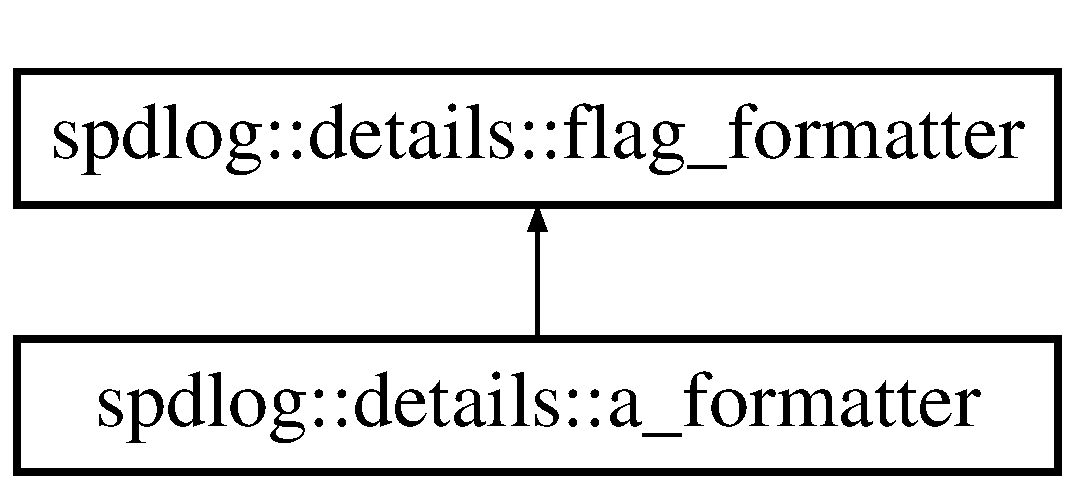
\includegraphics[height=2.000000cm]{classspdlog_1_1details_1_1a__formatter}
\end{center}
\end{figure}
\subsection*{Additional Inherited Members}


The documentation for this class was generated from the following file\+:\begin{DoxyCompactItemize}
\item 
cvdi-\/src/cvdi-\/cl/include/spdlog/details/pattern\+\_\+formatter\+\_\+impl.\+h\end{DoxyCompactItemize}

\hypertarget{structfmt_1_1AlignSpec}{}\section{fmt\+:\+:Align\+Spec Struct Reference}
\label{structfmt_1_1AlignSpec}\index{fmt\+::\+Align\+Spec@{fmt\+::\+Align\+Spec}}
Inheritance diagram for fmt\+:\+:Align\+Spec\+:\begin{figure}[H]
\begin{center}
\leavevmode
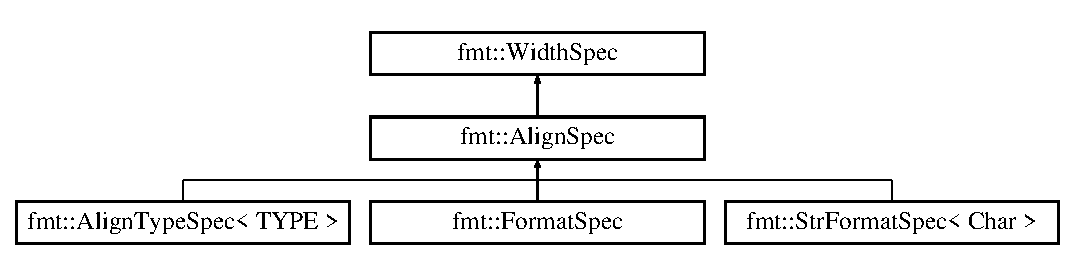
\includegraphics[height=3.000000cm]{structfmt_1_1AlignSpec}
\end{center}
\end{figure}
\subsection*{Public Member Functions}
\begin{DoxyCompactItemize}
\item 
{\bfseries Align\+Spec} (unsigned width, wchar\+\_\+t fill, Alignment align=A\+L\+I\+G\+N\+\_\+\+D\+E\+F\+A\+U\+LT)\hypertarget{structfmt_1_1AlignSpec_a7912b22ed62be96be0b9088b629f728c}{}\label{structfmt_1_1AlignSpec_a7912b22ed62be96be0b9088b629f728c}

\item 
Alignment {\bfseries align} () const \hypertarget{structfmt_1_1AlignSpec_abd14faffccf107e6e01bbd014e69262c}{}\label{structfmt_1_1AlignSpec_abd14faffccf107e6e01bbd014e69262c}

\item 
int {\bfseries precision} () const \hypertarget{structfmt_1_1AlignSpec_acdcb20e3a29b69355825ece5886db27b}{}\label{structfmt_1_1AlignSpec_acdcb20e3a29b69355825ece5886db27b}

\end{DoxyCompactItemize}
\subsection*{Public Attributes}
\begin{DoxyCompactItemize}
\item 
Alignment {\bfseries align\+\_\+}\hypertarget{structfmt_1_1AlignSpec_aac93fb3829d550af86479f1ecaa73f95}{}\label{structfmt_1_1AlignSpec_aac93fb3829d550af86479f1ecaa73f95}

\end{DoxyCompactItemize}


The documentation for this struct was generated from the following file\+:\begin{DoxyCompactItemize}
\item 
cvdi-\/src/cvdi-\/cl/include/spdlog/fmt/bundled/format.\+h\end{DoxyCompactItemize}

\hypertarget{structfmt_1_1AlignTypeSpec}{}\section{fmt\+:\+:Align\+Type\+Spec$<$ T\+Y\+PE $>$ Struct Template Reference}
\label{structfmt_1_1AlignTypeSpec}\index{fmt\+::\+Align\+Type\+Spec$<$ T\+Y\+P\+E $>$@{fmt\+::\+Align\+Type\+Spec$<$ T\+Y\+P\+E $>$}}
Inheritance diagram for fmt\+:\+:Align\+Type\+Spec$<$ T\+Y\+PE $>$\+:\begin{figure}[H]
\begin{center}
\leavevmode
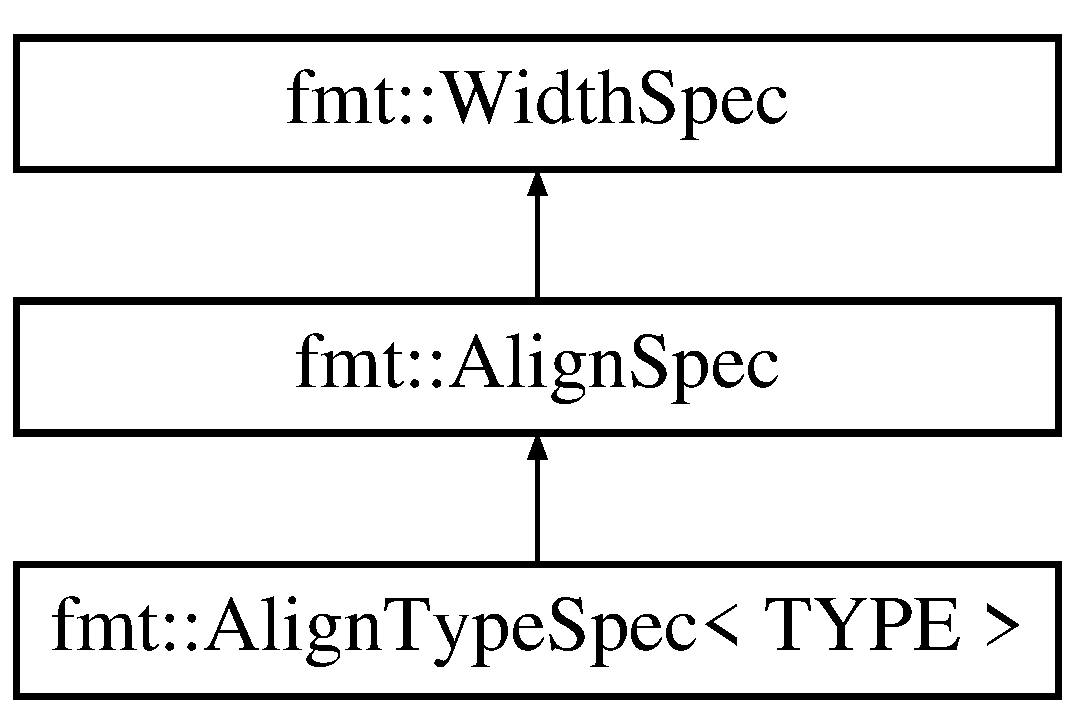
\includegraphics[height=3.000000cm]{structfmt_1_1AlignTypeSpec}
\end{center}
\end{figure}
\subsection*{Public Member Functions}
\begin{DoxyCompactItemize}
\item 
{\bfseries Align\+Type\+Spec} (unsigned width, wchar\+\_\+t fill)\hypertarget{structfmt_1_1AlignTypeSpec_a8140ef8fb8153a445ab7975fa2c30525}{}\label{structfmt_1_1AlignTypeSpec_a8140ef8fb8153a445ab7975fa2c30525}

\item 
bool {\bfseries flag} (unsigned) const \hypertarget{structfmt_1_1AlignTypeSpec_a20ab6ad809a76ea55d6f118526c25112}{}\label{structfmt_1_1AlignTypeSpec_a20ab6ad809a76ea55d6f118526c25112}

\item 
char {\bfseries type} () const \hypertarget{structfmt_1_1AlignTypeSpec_a15b451abb3309bcca720895faa320fe3}{}\label{structfmt_1_1AlignTypeSpec_a15b451abb3309bcca720895faa320fe3}

\end{DoxyCompactItemize}
\subsection*{Additional Inherited Members}


The documentation for this struct was generated from the following file\+:\begin{DoxyCompactItemize}
\item 
cvdi-\/src/cvdi-\/cl/include/spdlog/fmt/bundled/format.\+h\end{DoxyCompactItemize}

\hypertarget{classspdlog_1_1sinks_1_1ansicolor__sink}{}\section{spdlog\+:\+:sinks\+:\+:ansicolor\+\_\+sink$<$ Mutex $>$ Class Template Reference}
\label{classspdlog_1_1sinks_1_1ansicolor__sink}\index{spdlog\+::sinks\+::ansicolor\+\_\+sink$<$ Mutex $>$@{spdlog\+::sinks\+::ansicolor\+\_\+sink$<$ Mutex $>$}}


{\ttfamily \#include $<$ansicolor\+\_\+sink.\+h$>$}

Inheritance diagram for spdlog\+:\+:sinks\+:\+:ansicolor\+\_\+sink$<$ Mutex $>$\+:\begin{figure}[H]
\begin{center}
\leavevmode
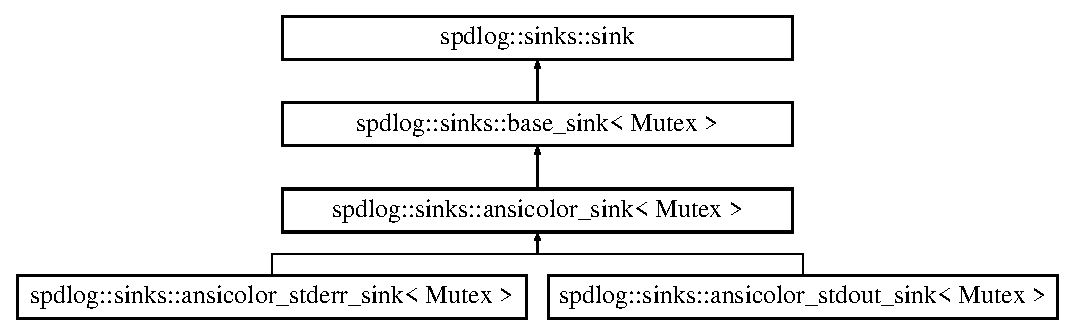
\includegraphics[height=4.000000cm]{classspdlog_1_1sinks_1_1ansicolor__sink}
\end{center}
\end{figure}
\subsection*{Public Member Functions}
\begin{DoxyCompactItemize}
\item 
{\bfseries ansicolor\+\_\+sink} (F\+I\+LE $\ast$file)\hypertarget{classspdlog_1_1sinks_1_1ansicolor__sink_af8bcfa424c86b13aa996724bc0a16e70}{}\label{classspdlog_1_1sinks_1_1ansicolor__sink_af8bcfa424c86b13aa996724bc0a16e70}

\end{DoxyCompactItemize}
\subsection*{Protected Member Functions}
\begin{DoxyCompactItemize}
\item 
virtual void {\bfseries \+\_\+sink\+\_\+it} (const \hyperlink{structspdlog_1_1details_1_1log__msg}{details\+::log\+\_\+msg} \&msg) override\hypertarget{classspdlog_1_1sinks_1_1ansicolor__sink_acda6ffd87c39e2828bc6af700d37b0f3}{}\label{classspdlog_1_1sinks_1_1ansicolor__sink_acda6ffd87c39e2828bc6af700d37b0f3}

\item 
void {\bfseries \+\_\+flush} () override\hypertarget{classspdlog_1_1sinks_1_1ansicolor__sink_a0e933cdbf08223904d80fde32f28d569}{}\label{classspdlog_1_1sinks_1_1ansicolor__sink_a0e933cdbf08223904d80fde32f28d569}

\end{DoxyCompactItemize}
\subsection*{Protected Attributes}
\begin{DoxyCompactItemize}
\item 
F\+I\+LE $\ast$ {\bfseries target\+\_\+file\+\_\+}\hypertarget{classspdlog_1_1sinks_1_1ansicolor__sink_abeea2ab4923f8bae0c74e0f65a1ebcd6}{}\label{classspdlog_1_1sinks_1_1ansicolor__sink_abeea2ab4923f8bae0c74e0f65a1ebcd6}

\item 
bool {\bfseries should\+\_\+do\+\_\+colors\+\_\+}\hypertarget{classspdlog_1_1sinks_1_1ansicolor__sink_a4d4ee5bb5b9953f5f150be371d8a9f0e}{}\label{classspdlog_1_1sinks_1_1ansicolor__sink_a4d4ee5bb5b9953f5f150be371d8a9f0e}

\item 
std\+::map$<$ level\+::level\+\_\+enum, std\+::string $>$ {\bfseries colors\+\_\+}\hypertarget{classspdlog_1_1sinks_1_1ansicolor__sink_a27337af3c5d95e97befd4dfc10a4ca60}{}\label{classspdlog_1_1sinks_1_1ansicolor__sink_a27337af3c5d95e97befd4dfc10a4ca60}

\end{DoxyCompactItemize}


\subsection{Detailed Description}
\subsubsection*{template$<$class Mutex$>$\\*
class spdlog\+::sinks\+::ansicolor\+\_\+sink$<$ Mutex $>$}

This sink prefixes the output with an A\+N\+SI escape sequence color code depending on the severity of the message. If no color terminal detected, omit the escape codes. 

The documentation for this class was generated from the following file\+:\begin{DoxyCompactItemize}
\item 
cvdi-\/src/cvdi-\/cl/include/spdlog/sinks/ansicolor\+\_\+sink.\+h\end{DoxyCompactItemize}

\hypertarget{classspdlog_1_1sinks_1_1ansicolor__stderr__sink}{}\section{spdlog\+:\+:sinks\+:\+:ansicolor\+\_\+stderr\+\_\+sink$<$ Mutex $>$ Class Template Reference}
\label{classspdlog_1_1sinks_1_1ansicolor__stderr__sink}\index{spdlog\+::sinks\+::ansicolor\+\_\+stderr\+\_\+sink$<$ Mutex $>$@{spdlog\+::sinks\+::ansicolor\+\_\+stderr\+\_\+sink$<$ Mutex $>$}}
Inheritance diagram for spdlog\+:\+:sinks\+:\+:ansicolor\+\_\+stderr\+\_\+sink$<$ Mutex $>$\+:\begin{figure}[H]
\begin{center}
\leavevmode
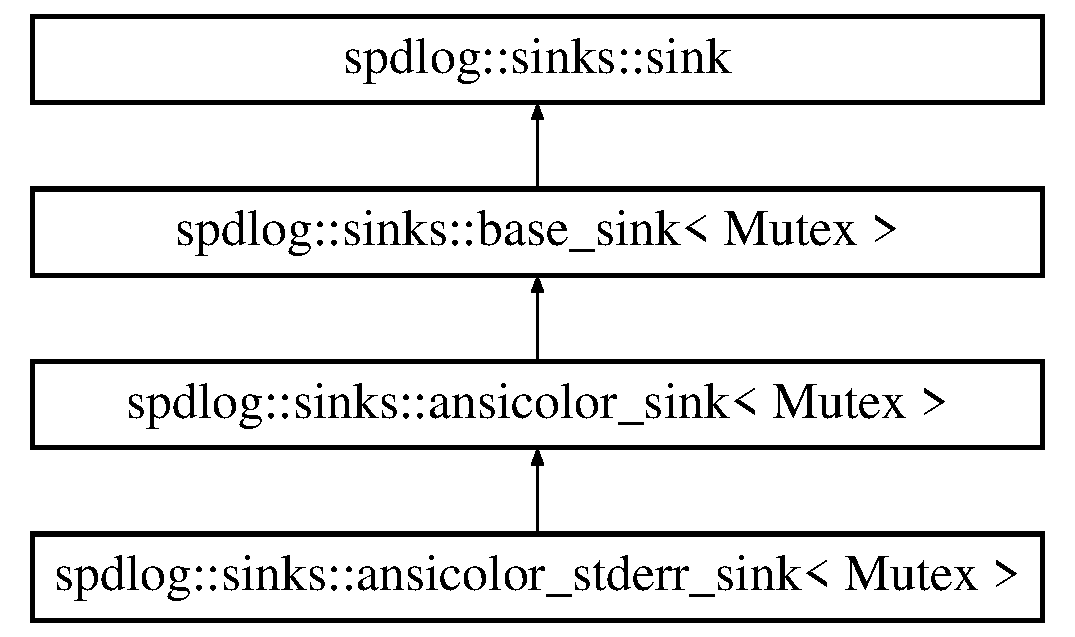
\includegraphics[height=4.000000cm]{classspdlog_1_1sinks_1_1ansicolor__stderr__sink}
\end{center}
\end{figure}
\subsection*{Additional Inherited Members}


The documentation for this class was generated from the following file\+:\begin{DoxyCompactItemize}
\item 
cvdi-\/src/cvdi-\/cl/include/spdlog/sinks/ansicolor\+\_\+sink.\+h\end{DoxyCompactItemize}

\hypertarget{classspdlog_1_1sinks_1_1ansicolor__stdout__sink}{}\section{spdlog\+:\+:sinks\+:\+:ansicolor\+\_\+stdout\+\_\+sink$<$ Mutex $>$ Class Template Reference}
\label{classspdlog_1_1sinks_1_1ansicolor__stdout__sink}\index{spdlog\+::sinks\+::ansicolor\+\_\+stdout\+\_\+sink$<$ Mutex $>$@{spdlog\+::sinks\+::ansicolor\+\_\+stdout\+\_\+sink$<$ Mutex $>$}}
Inheritance diagram for spdlog\+:\+:sinks\+:\+:ansicolor\+\_\+stdout\+\_\+sink$<$ Mutex $>$\+:\begin{figure}[H]
\begin{center}
\leavevmode
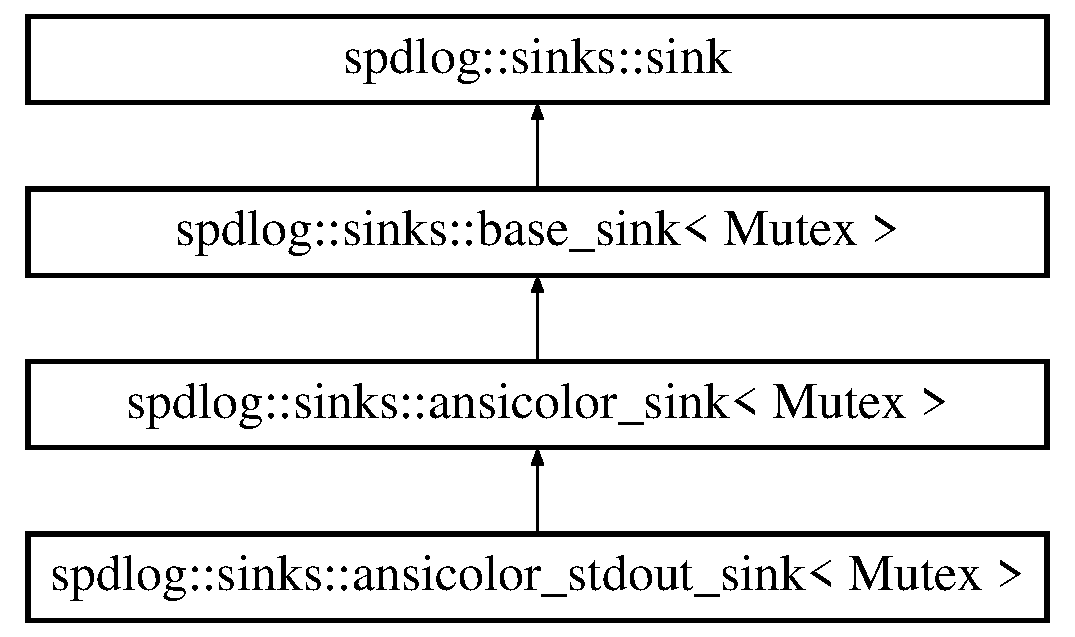
\includegraphics[height=4.000000cm]{classspdlog_1_1sinks_1_1ansicolor__stdout__sink}
\end{center}
\end{figure}
\subsection*{Additional Inherited Members}


The documentation for this class was generated from the following file\+:\begin{DoxyCompactItemize}
\item 
cvdi-\/src/cvdi-\/cl/include/spdlog/sinks/ansicolor\+\_\+sink.\+h\end{DoxyCompactItemize}

\hypertarget{classgeo_1_1Area}{}\section{geo\+:\+:Area Class Reference}
\label{classgeo_1_1Area}\index{geo\+::\+Area@{geo\+::\+Area}}


An \hyperlink{classgeo_1_1Area}{Area} object is a set of rectangular bounds used to check for geospatial point inclusion. Areas are constructed from line strings, where each segment has it\textquotesingle{}s own rectangular linear ring. Areas are invalid if the line string has less than 2 points, the width is less than or equal to zero, or the extension is less than zero.  




{\ttfamily \#include $<$geo.\+hpp$>$}

\subsection*{Public Types}
\begin{DoxyCompactItemize}
\item 
using {\bfseries Ptr} = std\+::shared\+\_\+ptr$<$ \hyperlink{classgeo_1_1Area}{Area} $>$\hypertarget{classgeo_1_1Area_ac41a4e39b3fd4614106df968a0b50850}{}\label{classgeo_1_1Area_ac41a4e39b3fd4614106df968a0b50850}

\end{DoxyCompactItemize}
\subsection*{Public Member Functions}
\begin{DoxyCompactItemize}
\item 
\hyperlink{classgeo_1_1Area_ade2820a667effacf5147a4873e52bba5}{Area} (const O\+G\+R\+Line\+String \&line\+\_\+string, double \hyperlink{classgeo_1_1Area_a2069d731b316767105af529c9473f3a6}{width}, double \hyperlink{classgeo_1_1Area_aded96bcf3e373315755f87579a10098a}{extension}=0.\+0)
\begin{DoxyCompactList}\small\item\em Construct an \hyperlink{classgeo_1_1Area}{Area} object from a line string with the given width and extension. The width and extension are applied to each rectangular, linear ring (line segment). \end{DoxyCompactList}\item 
double \hyperlink{classgeo_1_1Area_a2069d731b316767105af529c9473f3a6}{width} () const 
\begin{DoxyCompactList}\small\item\em Get the width of the area in meters. This is the width of each linear ring. \end{DoxyCompactList}\item 
double \hyperlink{classgeo_1_1Area_aded96bcf3e373315755f87579a10098a}{extension} () const 
\begin{DoxyCompactList}\small\item\em Get the extension of the area in meters. This is the length extension of each linear ring. \end{DoxyCompactList}\item 
bool \hyperlink{classgeo_1_1Area_ad802b7acb44e30984ec21018bca63460}{is\+\_\+valid} () const 
\begin{DoxyCompactList}\small\item\em Return true if the area is valid. Valid areas have at least one linear ring, a non-\/zero width, and a non-\/negative extension. \end{DoxyCompactList}\item 
bool \hyperlink{classgeo_1_1Area_a0bbd39e81f67912b91db243825594c45}{is\+\_\+within} (const O\+G\+R\+Point \&point) const 
\begin{DoxyCompactList}\small\item\em Return true if the given point is within the area. The point is within the area if it is within any of the area\textquotesingle{}s linear rings. \end{DoxyCompactList}\end{DoxyCompactItemize}
\subsection*{Public Attributes}
\begin{DoxyCompactItemize}
\item 
std\+::vector$<$ O\+G\+R\+Linear\+Ring $>$ \hyperlink{classgeo_1_1Area_a3e197ce947f9cc7df5c8ca93c97bb17f}{rings}\hypertarget{classgeo_1_1Area_a3e197ce947f9cc7df5c8ca93c97bb17f}{}\label{classgeo_1_1Area_a3e197ce947f9cc7df5c8ca93c97bb17f}

\begin{DoxyCompactList}\small\item\em The std\+::vector of O\+G\+R\+Linear\+Ring used to test for point inclusion. \end{DoxyCompactList}\end{DoxyCompactItemize}


\subsection{Detailed Description}
An \hyperlink{classgeo_1_1Area}{Area} object is a set of rectangular bounds used to check for geospatial point inclusion. Areas are constructed from line strings, where each segment has it\textquotesingle{}s own rectangular linear ring. Areas are invalid if the line string has less than 2 points, the width is less than or equal to zero, or the extension is less than zero. 

\subsection{Constructor \& Destructor Documentation}
\index{geo\+::\+Area@{geo\+::\+Area}!Area@{Area}}
\index{Area@{Area}!geo\+::\+Area@{geo\+::\+Area}}
\subsubsection[{\texorpdfstring{Area(const O\+G\+R\+Line\+String \&line\+\_\+string, double width, double extension=0.\+0)}{Area(const OGRLineString &line_string, double width, double extension=0.0)}}]{\setlength{\rightskip}{0pt plus 5cm}geo\+::\+Area\+::\+Area (
\begin{DoxyParamCaption}
\item[{const O\+G\+R\+Line\+String \&}]{line\+\_\+string, }
\item[{double}]{width, }
\item[{double}]{extension = {\ttfamily 0.0}}
\end{DoxyParamCaption}
)}\hypertarget{classgeo_1_1Area_ade2820a667effacf5147a4873e52bba5}{}\label{classgeo_1_1Area_ade2820a667effacf5147a4873e52bba5}


Construct an \hyperlink{classgeo_1_1Area}{Area} object from a line string with the given width and extension. The width and extension are applied to each rectangular, linear ring (line segment). 


\begin{DoxyParams}{Parameters}
{\em line\+\_\+string} & the line string from which to construct the area \\
\hline
{\em width} & the width of each linear ring in meters \\
\hline
{\em extension} & the length extension of each linear ring in meters \\
\hline
\end{DoxyParams}


\subsection{Member Function Documentation}
\index{geo\+::\+Area@{geo\+::\+Area}!extension@{extension}}
\index{extension@{extension}!geo\+::\+Area@{geo\+::\+Area}}
\subsubsection[{\texorpdfstring{extension() const }{extension() const }}]{\setlength{\rightskip}{0pt plus 5cm}double geo\+::\+Area\+::extension (
\begin{DoxyParamCaption}
{}
\end{DoxyParamCaption}
) const}\hypertarget{classgeo_1_1Area_aded96bcf3e373315755f87579a10098a}{}\label{classgeo_1_1Area_aded96bcf3e373315755f87579a10098a}


Get the extension of the area in meters. This is the length extension of each linear ring. 

\begin{DoxyReturn}{Returns}
the extension in meters 
\end{DoxyReturn}
\index{geo\+::\+Area@{geo\+::\+Area}!is\+\_\+valid@{is\+\_\+valid}}
\index{is\+\_\+valid@{is\+\_\+valid}!geo\+::\+Area@{geo\+::\+Area}}
\subsubsection[{\texorpdfstring{is\+\_\+valid() const }{is_valid() const }}]{\setlength{\rightskip}{0pt plus 5cm}bool geo\+::\+Area\+::is\+\_\+valid (
\begin{DoxyParamCaption}
{}
\end{DoxyParamCaption}
) const}\hypertarget{classgeo_1_1Area_ad802b7acb44e30984ec21018bca63460}{}\label{classgeo_1_1Area_ad802b7acb44e30984ec21018bca63460}


Return true if the area is valid. Valid areas have at least one linear ring, a non-\/zero width, and a non-\/negative extension. 

\begin{DoxyReturn}{Returns}
true if valid, otherwise false 
\end{DoxyReturn}
\index{geo\+::\+Area@{geo\+::\+Area}!is\+\_\+within@{is\+\_\+within}}
\index{is\+\_\+within@{is\+\_\+within}!geo\+::\+Area@{geo\+::\+Area}}
\subsubsection[{\texorpdfstring{is\+\_\+within(const O\+G\+R\+Point \&point) const }{is_within(const OGRPoint &point) const }}]{\setlength{\rightskip}{0pt plus 5cm}bool geo\+::\+Area\+::is\+\_\+within (
\begin{DoxyParamCaption}
\item[{const O\+G\+R\+Point \&}]{point}
\end{DoxyParamCaption}
) const}\hypertarget{classgeo_1_1Area_a0bbd39e81f67912b91db243825594c45}{}\label{classgeo_1_1Area_a0bbd39e81f67912b91db243825594c45}


Return true if the given point is within the area. The point is within the area if it is within any of the area\textquotesingle{}s linear rings. 


\begin{DoxyParams}{Parameters}
{\em point} & the point to check for inclusion \\
\hline
\end{DoxyParams}
\begin{DoxyReturn}{Returns}
true if the point is included, false otherwise 
\end{DoxyReturn}
\index{geo\+::\+Area@{geo\+::\+Area}!width@{width}}
\index{width@{width}!geo\+::\+Area@{geo\+::\+Area}}
\subsubsection[{\texorpdfstring{width() const }{width() const }}]{\setlength{\rightskip}{0pt plus 5cm}double geo\+::\+Area\+::width (
\begin{DoxyParamCaption}
{}
\end{DoxyParamCaption}
) const}\hypertarget{classgeo_1_1Area_a2069d731b316767105af529c9473f3a6}{}\label{classgeo_1_1Area_a2069d731b316767105af529c9473f3a6}


Get the width of the area in meters. This is the width of each linear ring. 

\begin{DoxyReturn}{Returns}
the width in meters 
\end{DoxyReturn}


The documentation for this class was generated from the following files\+:\begin{DoxyCompactItemize}
\item 
cvdi-\/src/geo/include/geo.\+hpp\item 
cvdi-\/src/geo/src/geo.\+cpp\end{DoxyCompactItemize}

\hypertarget{classcvdi_1_1AreaFitter}{}\section{cvdi\+:\+:Area\+Fitter Class Reference}
\label{classcvdi_1_1AreaFitter}\index{cvdi\+::\+Area\+Fitter@{cvdi\+::\+Area\+Fitter}}


Annotate a trace with fit area edges for each edge.  




{\ttfamily \#include $<$cvdi.\+hpp$>$}

\subsection*{Public Types}
\begin{DoxyCompactItemize}
\item 
using {\bfseries Area\+Set} = std\+::unordered\+\_\+set$<$ geo\+::\+Area\+::\+Ptr $>$\hypertarget{classcvdi_1_1AreaFitter_ae7be357d8b6c0156cb8bfedecd5feb0f}{}\label{classcvdi_1_1AreaFitter_ae7be357d8b6c0156cb8bfedecd5feb0f}

\end{DoxyCompactItemize}
\subsection*{Public Member Functions}
\begin{DoxyCompactItemize}
\item 
\hyperlink{classcvdi_1_1AreaFitter_a53040e056cbdc8b8862ad03b36158eed}{Area\+Fitter} (double fit\+\_\+width\+\_\+scaling=1.\+0, double fit\+\_\+extension=5.\+0, uint32\+\_\+t num\+\_\+sectors=36, uint32\+\_\+t min\+\_\+fit\+\_\+points=50)
\begin{DoxyCompactList}\small\item\em Construct an Area Fitter object. \end{DoxyCompactList}\item 
void \hyperlink{classcvdi_1_1AreaFitter_a8f4d6d9a5e4e27afbe9ea74cd52e5351}{fit} (geo\+\_\+data\+::\+Sample\+::\+Ptr sample)
\begin{DoxyCompactList}\small\item\em Fit a sample to a road area. \end{DoxyCompactList}\item 
void \hyperlink{classcvdi_1_1AreaFitter_a87669e87838bc1a3181e7b905c1967fa}{fit} (geo\+\_\+data\+::\+Sample\+::\+Trace \&trace)
\begin{DoxyCompactList}\small\item\em Fit an entire trace to road areas. \end{DoxyCompactList}\end{DoxyCompactItemize}
\subsection*{Public Attributes}
\begin{DoxyCompactItemize}
\item 
Edge\+Set \hyperlink{classcvdi_1_1AreaFitter_a362bc13dadb5e7ff3151bbf8d0fe735c}{implicit\+\_\+edge\+\_\+set}\hypertarget{classcvdi_1_1AreaFitter_a362bc13dadb5e7ff3151bbf8d0fe735c}{}\label{classcvdi_1_1AreaFitter_a362bc13dadb5e7ff3151bbf8d0fe735c}

\begin{DoxyCompactList}\small\item\em The complete set of implicit edges. \end{DoxyCompactList}\item 
Edge\+Set \hyperlink{classcvdi_1_1AreaFitter_a60a8f1de63afe94f368a06382a035acb}{explicit\+\_\+edge\+\_\+set}\hypertarget{classcvdi_1_1AreaFitter_a60a8f1de63afe94f368a06382a035acb}{}\label{classcvdi_1_1AreaFitter_a60a8f1de63afe94f368a06382a035acb}

\begin{DoxyCompactList}\small\item\em The complete set of implicit edges. \end{DoxyCompactList}\item 
Area\+Set \hyperlink{classcvdi_1_1AreaFitter_a51b64f5f4d531e6ca4bc03b554f77c7e}{implicit\+\_\+area\+\_\+set}\hypertarget{classcvdi_1_1AreaFitter_a51b64f5f4d531e6ca4bc03b554f77c7e}{}\label{classcvdi_1_1AreaFitter_a51b64f5f4d531e6ca4bc03b554f77c7e}

\begin{DoxyCompactList}\small\item\em The complete set of areas built from the implicit edges. \end{DoxyCompactList}\item 
Area\+Set \hyperlink{classcvdi_1_1AreaFitter_afaca52e1741b02ba88960cb3b837b8f4}{explicit\+\_\+area\+\_\+set}\hypertarget{classcvdi_1_1AreaFitter_afaca52e1741b02ba88960cb3b837b8f4}{}\label{classcvdi_1_1AreaFitter_afaca52e1741b02ba88960cb3b837b8f4}

\begin{DoxyCompactList}\small\item\em The complete set of areas built from the implicit edges. \end{DoxyCompactList}\end{DoxyCompactItemize}


\subsection{Detailed Description}
Annotate a trace with fit area edges for each edge. 

\subsection{Constructor \& Destructor Documentation}
\index{cvdi\+::\+Area\+Fitter@{cvdi\+::\+Area\+Fitter}!Area\+Fitter@{Area\+Fitter}}
\index{Area\+Fitter@{Area\+Fitter}!cvdi\+::\+Area\+Fitter@{cvdi\+::\+Area\+Fitter}}
\subsubsection[{\texorpdfstring{Area\+Fitter(double fit\+\_\+width\+\_\+scaling=1.\+0, double fit\+\_\+extension=5.\+0, uint32\+\_\+t num\+\_\+sectors=36, uint32\+\_\+t min\+\_\+fit\+\_\+points=50)}{AreaFitter(double fit_width_scaling=1.0, double fit_extension=5.0, uint32_t num_sectors=36, uint32_t min_fit_points=50)}}]{\setlength{\rightskip}{0pt plus 5cm}cvdi\+::\+Area\+Fitter\+::\+Area\+Fitter (
\begin{DoxyParamCaption}
\item[{double}]{fit\+\_\+width\+\_\+scaling = {\ttfamily 1.0}, }
\item[{double}]{fit\+\_\+extension = {\ttfamily 5.0}, }
\item[{uint32\+\_\+t}]{num\+\_\+sectors = {\ttfamily 36}, }
\item[{uint32\+\_\+t}]{min\+\_\+fit\+\_\+points = {\ttfamily 50}}
\end{DoxyParamCaption}
)}\hypertarget{classcvdi_1_1AreaFitter_a53040e056cbdc8b8862ad03b36158eed}{}\label{classcvdi_1_1AreaFitter_a53040e056cbdc8b8862ad03b36158eed}


Construct an Area Fitter object. 


\begin{DoxyParams}{Parameters}
{\em num\+\_\+sectors} & the compass rose is divided into this number of equally sized sectors \\
\hline
{\em min\+\_\+fit\+\_\+points} & use no less than this many points to infer a road segment \\
\hline
\end{DoxyParams}


\subsection{Member Function Documentation}
\index{cvdi\+::\+Area\+Fitter@{cvdi\+::\+Area\+Fitter}!fit@{fit}}
\index{fit@{fit}!cvdi\+::\+Area\+Fitter@{cvdi\+::\+Area\+Fitter}}
\subsubsection[{\texorpdfstring{fit(geo\+\_\+data\+::\+Sample\+::\+Ptr sample)}{fit(geo_data::Sample::Ptr sample)}}]{\setlength{\rightskip}{0pt plus 5cm}void cvdi\+::\+Area\+Fitter\+::fit (
\begin{DoxyParamCaption}
\item[{geo\+\_\+data\+::\+Sample\+::\+Ptr}]{sample}
\end{DoxyParamCaption}
)}\hypertarget{classcvdi_1_1AreaFitter_a8f4d6d9a5e4e27afbe9ea74cd52e5351}{}\label{classcvdi_1_1AreaFitter_a8f4d6d9a5e4e27afbe9ea74cd52e5351}


Fit a sample to a road area. 


\begin{DoxyParams}{Parameters}
{\em sample} & pointer to a \hyperlink{classgeo__data_1_1Sample}{geo\+\_\+data\+::\+Sample} \\
\hline
\end{DoxyParams}
\index{cvdi\+::\+Area\+Fitter@{cvdi\+::\+Area\+Fitter}!fit@{fit}}
\index{fit@{fit}!cvdi\+::\+Area\+Fitter@{cvdi\+::\+Area\+Fitter}}
\subsubsection[{\texorpdfstring{fit(geo\+\_\+data\+::\+Sample\+::\+Trace \&trace)}{fit(geo_data::Sample::Trace &trace)}}]{\setlength{\rightskip}{0pt plus 5cm}void cvdi\+::\+Area\+Fitter\+::fit (
\begin{DoxyParamCaption}
\item[{geo\+\_\+data\+::\+Sample\+::\+Trace \&}]{trace}
\end{DoxyParamCaption}
)}\hypertarget{classcvdi_1_1AreaFitter_a87669e87838bc1a3181e7b905c1967fa}{}\label{classcvdi_1_1AreaFitter_a87669e87838bc1a3181e7b905c1967fa}


Fit an entire trace to road areas. 


\begin{DoxyParams}{Parameters}
{\em trace} & the trace to fit \\
\hline
\end{DoxyParams}


The documentation for this class was generated from the following files\+:\begin{DoxyCompactItemize}
\item 
cvdi-\/src/cvdi/include/cvdi.\+hpp\item 
cvdi-\/src/cvdi/src/cvdi.\+cpp\end{DoxyCompactItemize}

\hypertarget{structfmt_1_1internal_1_1Arg}{}\section{fmt\+:\+:internal\+:\+:Arg Struct Reference}
\label{structfmt_1_1internal_1_1Arg}\index{fmt\+::internal\+::\+Arg@{fmt\+::internal\+::\+Arg}}
Inheritance diagram for fmt\+:\+:internal\+:\+:Arg\+:\begin{figure}[H]
\begin{center}
\leavevmode
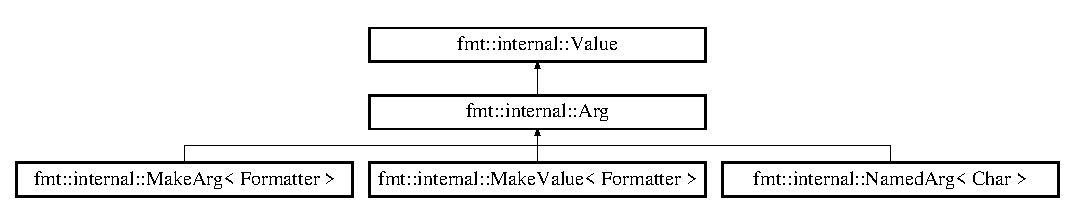
\includegraphics[height=2.413793cm]{structfmt_1_1internal_1_1Arg}
\end{center}
\end{figure}
\subsection*{Public Attributes}
\begin{DoxyCompactItemize}
\item 
Type {\bfseries type}\hypertarget{structfmt_1_1internal_1_1Arg_af1165b4e8647bea5913922de82599e2e}{}\label{structfmt_1_1internal_1_1Arg_af1165b4e8647bea5913922de82599e2e}

\end{DoxyCompactItemize}
\subsection*{Additional Inherited Members}


The documentation for this struct was generated from the following file\+:\begin{DoxyCompactItemize}
\item 
cvdi-\/src/cvdi-\/cl/include/spdlog/fmt/bundled/format.\+h\end{DoxyCompactItemize}

\hypertarget{structfmt_1_1internal_1_1ArgArray}{}\section{fmt\+:\+:internal\+:\+:Arg\+Array$<$ N, bool $>$ Struct Template Reference}
\label{structfmt_1_1internal_1_1ArgArray}\index{fmt\+::internal\+::\+Arg\+Array$<$ N, bool $>$@{fmt\+::internal\+::\+Arg\+Array$<$ N, bool $>$}}


The documentation for this struct was generated from the following file\+:\begin{DoxyCompactItemize}
\item 
cvdi-\/src/cvdi-\/cl/include/spdlog/fmt/bundled/format.\+h\end{DoxyCompactItemize}

\hypertarget{structfmt_1_1internal_1_1ArgArray_3_01N_00_01false_01_4}{}\section{fmt\+:\+:internal\+:\+:Arg\+Array$<$ N, false $>$ Struct Template Reference}
\label{structfmt_1_1internal_1_1ArgArray_3_01N_00_01false_01_4}\index{fmt\+::internal\+::\+Arg\+Array$<$ N, false $>$@{fmt\+::internal\+::\+Arg\+Array$<$ N, false $>$}}
\subsection*{Public Types}
\begin{DoxyCompactItemize}
\item 
typedef \hyperlink{structfmt_1_1internal_1_1Arg}{Arg} {\bfseries Type}\mbox{[}N+1\mbox{]}\hypertarget{structfmt_1_1internal_1_1ArgArray_3_01N_00_01false_01_4_ab53fffd4174d8cdc70c205ba6dc54b17}{}\label{structfmt_1_1internal_1_1ArgArray_3_01N_00_01false_01_4_ab53fffd4174d8cdc70c205ba6dc54b17}

\end{DoxyCompactItemize}
\subsection*{Static Public Member Functions}
\begin{DoxyCompactItemize}
\item 
{\footnotesize template$<$typename Formatter , typename T $>$ }\\static \hyperlink{structfmt_1_1internal_1_1Arg}{Arg} {\bfseries make} (const T \&value)\hypertarget{structfmt_1_1internal_1_1ArgArray_3_01N_00_01false_01_4_a5052e0376e3deb4bffc5d1a4941bc7c8}{}\label{structfmt_1_1internal_1_1ArgArray_3_01N_00_01false_01_4_a5052e0376e3deb4bffc5d1a4941bc7c8}

\end{DoxyCompactItemize}


The documentation for this struct was generated from the following file\+:\begin{DoxyCompactItemize}
\item 
cvdi-\/src/cvdi-\/cl/include/spdlog/fmt/bundled/format.\+h\end{DoxyCompactItemize}

\hypertarget{structfmt_1_1internal_1_1ArgArray_3_01N_00_01true_01_4}{}\section{fmt\+:\+:internal\+:\+:Arg\+Array$<$ N, true $>$ Struct Template Reference}
\label{structfmt_1_1internal_1_1ArgArray_3_01N_00_01true_01_4}\index{fmt\+::internal\+::\+Arg\+Array$<$ N, true $>$@{fmt\+::internal\+::\+Arg\+Array$<$ N, true $>$}}
\subsection*{Public Types}
\begin{DoxyCompactItemize}
\item 
typedef \hyperlink{structfmt_1_1internal_1_1Value}{Value} {\bfseries Type}\mbox{[}N $>$ 0?N\+:1\mbox{]}\hypertarget{structfmt_1_1internal_1_1ArgArray_3_01N_00_01true_01_4_aeb168342e5c7353d8780f936d393c04f}{}\label{structfmt_1_1internal_1_1ArgArray_3_01N_00_01true_01_4_aeb168342e5c7353d8780f936d393c04f}

\end{DoxyCompactItemize}
\subsection*{Static Public Member Functions}
\begin{DoxyCompactItemize}
\item 
{\footnotesize template$<$typename Formatter , typename T $>$ }\\static \hyperlink{structfmt_1_1internal_1_1Value}{Value} {\bfseries make} (const T \&value)\hypertarget{structfmt_1_1internal_1_1ArgArray_3_01N_00_01true_01_4_a3977c938e1ca5c4c5aedccd85561a76d}{}\label{structfmt_1_1internal_1_1ArgArray_3_01N_00_01true_01_4_a3977c938e1ca5c4c5aedccd85561a76d}

\end{DoxyCompactItemize}


The documentation for this struct was generated from the following file\+:\begin{DoxyCompactItemize}
\item 
cvdi-\/src/cvdi-\/cl/include/spdlog/fmt/bundled/format.\+h\end{DoxyCompactItemize}

\hypertarget{classfmt_1_1ArgFormatter}{}\section{fmt\+:\+:Arg\+Formatter$<$ Char $>$ Class Template Reference}
\label{classfmt_1_1ArgFormatter}\index{fmt\+::\+Arg\+Formatter$<$ Char $>$@{fmt\+::\+Arg\+Formatter$<$ Char $>$}}


{\ttfamily \#include $<$format.\+h$>$}

Inheritance diagram for fmt\+:\+:Arg\+Formatter$<$ Char $>$\+:\begin{figure}[H]
\begin{center}
\leavevmode
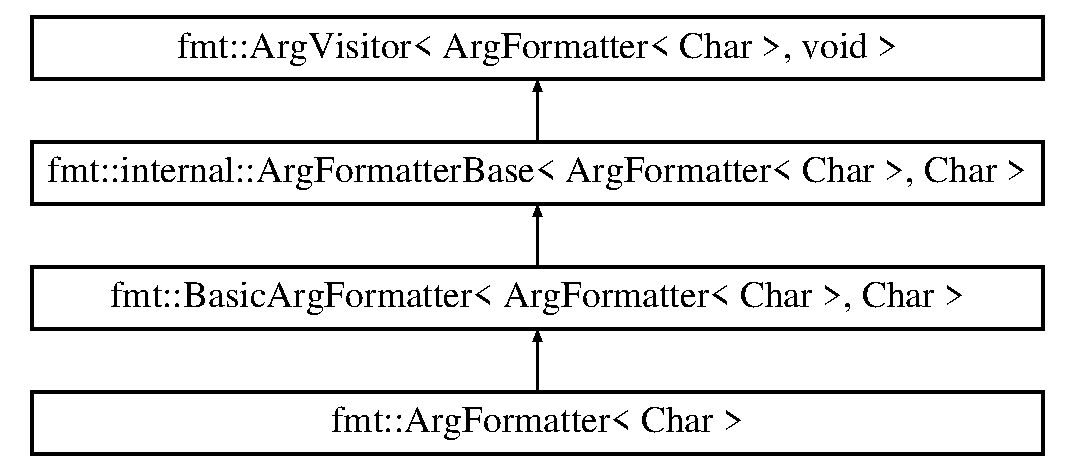
\includegraphics[height=4.000000cm]{classfmt_1_1ArgFormatter}
\end{center}
\end{figure}
\subsection*{Public Member Functions}
\begin{DoxyCompactItemize}
\item 
\hyperlink{classfmt_1_1ArgFormatter_a2fc7b9c801f3aa33a8e952df035a140f}{Arg\+Formatter} (\hyperlink{classfmt_1_1BasicFormatter}{Basic\+Formatter}$<$ Char $>$ \&formatter, \hyperlink{structfmt_1_1FormatSpec}{Format\+Spec} \&spec, const Char $\ast$fmt)
\end{DoxyCompactItemize}
\subsection*{Additional Inherited Members}


\subsection{Detailed Description}
\subsubsection*{template$<$typename Char$>$\\*
class fmt\+::\+Arg\+Formatter$<$ Char $>$}

The default argument formatter. 

\subsection{Constructor \& Destructor Documentation}
\index{fmt\+::\+Arg\+Formatter@{fmt\+::\+Arg\+Formatter}!Arg\+Formatter@{Arg\+Formatter}}
\index{Arg\+Formatter@{Arg\+Formatter}!fmt\+::\+Arg\+Formatter@{fmt\+::\+Arg\+Formatter}}
\subsubsection[{\texorpdfstring{Arg\+Formatter(\+Basic\+Formatter$<$ Char $>$ \&formatter, Format\+Spec \&spec, const Char $\ast$fmt)}{ArgFormatter(BasicFormatter< Char > &formatter, FormatSpec &spec, const Char *fmt)}}]{\setlength{\rightskip}{0pt plus 5cm}template$<$typename Char $>$ {\bf fmt\+::\+Arg\+Formatter}$<$ Char $>$\+::{\bf Arg\+Formatter} (
\begin{DoxyParamCaption}
\item[{{\bf Basic\+Formatter}$<$ Char $>$ \&}]{formatter, }
\item[{{\bf Format\+Spec} \&}]{spec, }
\item[{const Char $\ast$}]{fmt}
\end{DoxyParamCaption}
)\hspace{0.3cm}{\ttfamily [inline]}}\hypertarget{classfmt_1_1ArgFormatter_a2fc7b9c801f3aa33a8e952df035a140f}{}\label{classfmt_1_1ArgFormatter_a2fc7b9c801f3aa33a8e952df035a140f}
Constructs an argument formatter object. 

The documentation for this class was generated from the following file\+:\begin{DoxyCompactItemize}
\item 
cvdi-\/src/cvdi-\/cl/include/spdlog/fmt/bundled/format.\+h\end{DoxyCompactItemize}

\hypertarget{classfmt_1_1internal_1_1ArgFormatterBase}{}\section{fmt\+:\+:internal\+:\+:Arg\+Formatter\+Base$<$ Impl, Char $>$ Class Template Reference}
\label{classfmt_1_1internal_1_1ArgFormatterBase}\index{fmt\+::internal\+::\+Arg\+Formatter\+Base$<$ Impl, Char $>$@{fmt\+::internal\+::\+Arg\+Formatter\+Base$<$ Impl, Char $>$}}
Inheritance diagram for fmt\+:\+:internal\+:\+:Arg\+Formatter\+Base$<$ Impl, Char $>$\+:\begin{figure}[H]
\begin{center}
\leavevmode
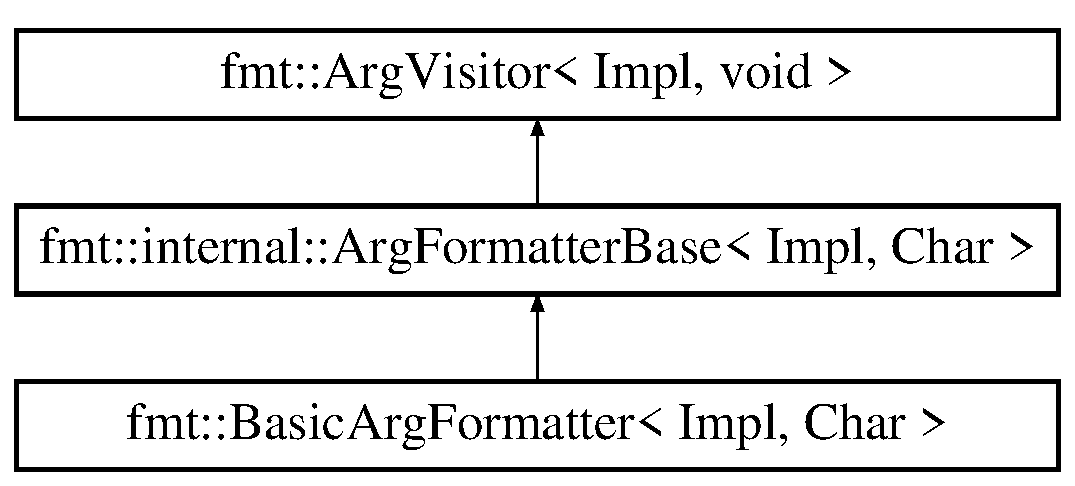
\includegraphics[height=3.000000cm]{classfmt_1_1internal_1_1ArgFormatterBase}
\end{center}
\end{figure}
\subsection*{Public Member Functions}
\begin{DoxyCompactItemize}
\item 
{\bfseries Arg\+Formatter\+Base} (\hyperlink{classfmt_1_1BasicWriter}{Basic\+Writer}$<$ Char $>$ \&w, \hyperlink{structfmt_1_1FormatSpec}{Format\+Spec} \&s)\hypertarget{classfmt_1_1internal_1_1ArgFormatterBase_a67f48acedb2ba3f243150c41f964252b}{}\label{classfmt_1_1internal_1_1ArgFormatterBase_a67f48acedb2ba3f243150c41f964252b}

\item 
{\footnotesize template$<$typename T $>$ }\\void {\bfseries visit\+\_\+any\+\_\+int} (T value)\hypertarget{classfmt_1_1internal_1_1ArgFormatterBase_ae6f9ce1fa7940ebda3ac594a45edd32d}{}\label{classfmt_1_1internal_1_1ArgFormatterBase_ae6f9ce1fa7940ebda3ac594a45edd32d}

\item 
{\footnotesize template$<$typename T $>$ }\\void {\bfseries visit\+\_\+any\+\_\+double} (T value)\hypertarget{classfmt_1_1internal_1_1ArgFormatterBase_a670214e1773c9c86002be07c043566dd}{}\label{classfmt_1_1internal_1_1ArgFormatterBase_a670214e1773c9c86002be07c043566dd}

\item 
void {\bfseries visit\+\_\+bool} (bool value)\hypertarget{classfmt_1_1internal_1_1ArgFormatterBase_a379b2f30d3e0526c88be65f8a2b596be}{}\label{classfmt_1_1internal_1_1ArgFormatterBase_a379b2f30d3e0526c88be65f8a2b596be}

\item 
void {\bfseries visit\+\_\+char} (int value)\hypertarget{classfmt_1_1internal_1_1ArgFormatterBase_ab85eb2158c9d48c847706de26f35460c}{}\label{classfmt_1_1internal_1_1ArgFormatterBase_ab85eb2158c9d48c847706de26f35460c}

\item 
void {\bfseries visit\+\_\+cstring} (const char $\ast$value)\hypertarget{classfmt_1_1internal_1_1ArgFormatterBase_a35e5c4d1580f7eec032661f9823c0cad}{}\label{classfmt_1_1internal_1_1ArgFormatterBase_a35e5c4d1580f7eec032661f9823c0cad}

\item 
void {\bfseries visit\+\_\+string} (\hyperlink{structfmt_1_1internal_1_1Value_1_1StringValue}{Arg\+::\+String\+Value}$<$ char $>$ value)\hypertarget{classfmt_1_1internal_1_1ArgFormatterBase_a937a7808ebf21736498e32abba6a0046}{}\label{classfmt_1_1internal_1_1ArgFormatterBase_a937a7808ebf21736498e32abba6a0046}

\item 
void {\bfseries visit\+\_\+wstring} (\hyperlink{structfmt_1_1internal_1_1Value_1_1StringValue}{Arg\+::\+String\+Value}$<$ Char $>$ value)\hypertarget{classfmt_1_1internal_1_1ArgFormatterBase_ad3469bff1ffe51395d9f8f0e0824ff2c}{}\label{classfmt_1_1internal_1_1ArgFormatterBase_ad3469bff1ffe51395d9f8f0e0824ff2c}

\item 
void {\bfseries visit\+\_\+pointer} (const void $\ast$value)\hypertarget{classfmt_1_1internal_1_1ArgFormatterBase_a5c11af21a3e1249b78ef87c968572ef5}{}\label{classfmt_1_1internal_1_1ArgFormatterBase_a5c11af21a3e1249b78ef87c968572ef5}

\end{DoxyCompactItemize}
\subsection*{Protected Member Functions}
\begin{DoxyCompactItemize}
\item 
\hyperlink{classfmt_1_1BasicWriter}{Basic\+Writer}$<$ Char $>$ \& {\bfseries writer} ()\hypertarget{classfmt_1_1internal_1_1ArgFormatterBase_a042c1243143197b04c5b4d77a89a4fb5}{}\label{classfmt_1_1internal_1_1ArgFormatterBase_a042c1243143197b04c5b4d77a89a4fb5}

\item 
\hyperlink{structfmt_1_1FormatSpec}{Format\+Spec} \& {\bfseries spec} ()\hypertarget{classfmt_1_1internal_1_1ArgFormatterBase_acdd3bb185f7b444a60faf98fa9806ed4}{}\label{classfmt_1_1internal_1_1ArgFormatterBase_acdd3bb185f7b444a60faf98fa9806ed4}

\item 
void {\bfseries write} (bool value)\hypertarget{classfmt_1_1internal_1_1ArgFormatterBase_a002d52aca6bc9a70d7eb62c037ffadc4}{}\label{classfmt_1_1internal_1_1ArgFormatterBase_a002d52aca6bc9a70d7eb62c037ffadc4}

\item 
void {\bfseries write} (const char $\ast$value)\hypertarget{classfmt_1_1internal_1_1ArgFormatterBase_a1a706cd6067d51bfa07d5e6c577e0843}{}\label{classfmt_1_1internal_1_1ArgFormatterBase_a1a706cd6067d51bfa07d5e6c577e0843}

\end{DoxyCompactItemize}


The documentation for this class was generated from the following file\+:\begin{DoxyCompactItemize}
\item 
cvdi-\/src/cvdi-\/cl/include/spdlog/fmt/bundled/format.\+h\end{DoxyCompactItemize}

\hypertarget{classfmt_1_1ArgList}{}\section{fmt\+:\+:Arg\+List Class Reference}
\label{classfmt_1_1ArgList}\index{fmt\+::\+Arg\+List@{fmt\+::\+Arg\+List}}


{\ttfamily \#include $<$format.\+h$>$}

\subsection*{Public Types}
\begin{DoxyCompactItemize}
\item 
enum \{ {\bfseries M\+A\+X\+\_\+\+P\+A\+C\+K\+E\+D\+\_\+\+A\+R\+GS} = 16
 \}\hypertarget{classfmt_1_1ArgList_a4023f9c6f9dc0cb62d97f8fecc702d7c}{}\label{classfmt_1_1ArgList_a4023f9c6f9dc0cb62d97f8fecc702d7c}

\end{DoxyCompactItemize}
\subsection*{Public Member Functions}
\begin{DoxyCompactItemize}
\item 
{\bfseries Arg\+List} (U\+Long\+Long types, const \hyperlink{structfmt_1_1internal_1_1Value}{internal\+::\+Value} $\ast$values)\hypertarget{classfmt_1_1ArgList_a02125120a594f45fdad426ef003aa342}{}\label{classfmt_1_1ArgList_a02125120a594f45fdad426ef003aa342}

\item 
{\bfseries Arg\+List} (U\+Long\+Long types, const \hyperlink{structfmt_1_1internal_1_1Arg}{internal\+::\+Arg} $\ast$args)\hypertarget{classfmt_1_1ArgList_ae811ca8034f8c88fe612e0d23ae810fe}{}\label{classfmt_1_1ArgList_ae811ca8034f8c88fe612e0d23ae810fe}

\item 
\hyperlink{structfmt_1_1internal_1_1Arg}{internal\+::\+Arg} \hyperlink{classfmt_1_1ArgList_ad2c2672388e003aa70d9c948ac8140cd}{operator\mbox{[}$\,$\mbox{]}} (unsigned index) const 
\end{DoxyCompactItemize}
\subsection*{Friends}
\begin{DoxyCompactItemize}
\item 
{\footnotesize template$<$typename Char $>$ }\\class {\bfseries internal\+::\+Arg\+Map}\hypertarget{classfmt_1_1ArgList_a6e257e0433f829293f077ba81f205ab3}{}\label{classfmt_1_1ArgList_a6e257e0433f829293f077ba81f205ab3}

\end{DoxyCompactItemize}


\subsection{Detailed Description}
An argument list. 

\subsection{Member Function Documentation}
\index{fmt\+::\+Arg\+List@{fmt\+::\+Arg\+List}!operator\mbox{[}$\,$\mbox{]}@{operator[]}}
\index{operator\mbox{[}$\,$\mbox{]}@{operator[]}!fmt\+::\+Arg\+List@{fmt\+::\+Arg\+List}}
\subsubsection[{\texorpdfstring{operator[](unsigned index) const }{operator[](unsigned index) const }}]{\setlength{\rightskip}{0pt plus 5cm}{\bf internal\+::\+Arg} fmt\+::\+Arg\+List\+::operator\mbox{[}$\,$\mbox{]} (
\begin{DoxyParamCaption}
\item[{unsigned}]{index}
\end{DoxyParamCaption}
) const\hspace{0.3cm}{\ttfamily [inline]}}\hypertarget{classfmt_1_1ArgList_ad2c2672388e003aa70d9c948ac8140cd}{}\label{classfmt_1_1ArgList_ad2c2672388e003aa70d9c948ac8140cd}
Returns the argument at specified index. 

The documentation for this class was generated from the following file\+:\begin{DoxyCompactItemize}
\item 
cvdi-\/src/cvdi-\/cl/include/spdlog/fmt/bundled/format.\+h\end{DoxyCompactItemize}

\hypertarget{classfmt_1_1internal_1_1ArgMap}{}\section{fmt\+:\+:internal\+:\+:Arg\+Map$<$ Char $>$ Class Template Reference}
\label{classfmt_1_1internal_1_1ArgMap}\index{fmt\+::internal\+::\+Arg\+Map$<$ Char $>$@{fmt\+::internal\+::\+Arg\+Map$<$ Char $>$}}
\subsection*{Public Member Functions}
\begin{DoxyCompactItemize}
\item 
F\+M\+T\+\_\+\+A\+PI void {\bfseries init} (const \hyperlink{classfmt_1_1ArgList}{Arg\+List} \&args)\hypertarget{classfmt_1_1internal_1_1ArgMap_aba1e77b1b5358a8e354acae3d71ea6cf}{}\label{classfmt_1_1internal_1_1ArgMap_aba1e77b1b5358a8e354acae3d71ea6cf}

\item 
const \hyperlink{structfmt_1_1internal_1_1Arg}{internal\+::\+Arg} $\ast$ {\bfseries find} (const \hyperlink{classfmt_1_1BasicStringRef}{fmt\+::\+Basic\+String\+Ref}$<$ Char $>$ \&name) const \hypertarget{classfmt_1_1internal_1_1ArgMap_a588b3169b52f72f8958a53a5f440a401}{}\label{classfmt_1_1internal_1_1ArgMap_a588b3169b52f72f8958a53a5f440a401}

\end{DoxyCompactItemize}


The documentation for this class was generated from the following files\+:\begin{DoxyCompactItemize}
\item 
cvdi-\/src/cvdi-\/cl/include/spdlog/fmt/bundled/format.\+h\item 
cvdi-\/src/cvdi-\/cl/include/spdlog/fmt/bundled/format.\+cc\end{DoxyCompactItemize}

\hypertarget{structfmt_1_1internal_1_1ArgType}{}\section{fmt\+:\+:internal\+:\+:Arg\+Type Struct Reference}
\label{structfmt_1_1internal_1_1ArgType}\index{fmt\+::internal\+::\+Arg\+Type@{fmt\+::internal\+::\+Arg\+Type}}
\subsection*{Public Member Functions}
\begin{DoxyCompactItemize}
\item 
{\footnotesize template$<$typename T $>$ }\\{\bfseries Arg\+Type} (const T \&arg)\hypertarget{structfmt_1_1internal_1_1ArgType_a011f9d3d3e6da48d17967466c3d94fc8}{}\label{structfmt_1_1internal_1_1ArgType_a011f9d3d3e6da48d17967466c3d94fc8}

\end{DoxyCompactItemize}
\subsection*{Public Attributes}
\begin{DoxyCompactItemize}
\item 
uint64\+\_\+t {\bfseries type}\hypertarget{structfmt_1_1internal_1_1ArgType_acfa7078681b7047cb448d523f5eb2a54}{}\label{structfmt_1_1internal_1_1ArgType_acfa7078681b7047cb448d523f5eb2a54}

\end{DoxyCompactItemize}


The documentation for this struct was generated from the following file\+:\begin{DoxyCompactItemize}
\item 
cvdi-\/src/cvdi-\/cl/include/spdlog/fmt/bundled/format.\+h\end{DoxyCompactItemize}

\hypertarget{classfmt_1_1ArgVisitor}{}\section{fmt\+:\+:Arg\+Visitor$<$ Impl, Result $>$ Class Template Reference}
\label{classfmt_1_1ArgVisitor}\index{fmt\+::\+Arg\+Visitor$<$ Impl, Result $>$@{fmt\+::\+Arg\+Visitor$<$ Impl, Result $>$}}


{\ttfamily \#include $<$format.\+h$>$}

\subsection*{Public Member Functions}
\begin{DoxyCompactItemize}
\item 
void {\bfseries report\+\_\+unhandled\+\_\+arg} ()\hypertarget{classfmt_1_1ArgVisitor_a130090f53213407548d93d8ee2801738}{}\label{classfmt_1_1ArgVisitor_a130090f53213407548d93d8ee2801738}

\item 
Result {\bfseries visit\+\_\+unhandled\+\_\+arg} ()\hypertarget{classfmt_1_1ArgVisitor_a8de54a54b863eb63b5c45c4495c12793}{}\label{classfmt_1_1ArgVisitor_a8de54a54b863eb63b5c45c4495c12793}

\item 
Result \hyperlink{classfmt_1_1ArgVisitor_ac6d79e3d931a9f56f40bca08f8651cdf}{visit\+\_\+int} (int value)
\item 
Result \hyperlink{classfmt_1_1ArgVisitor_ab5687cccaae516d3e6e94775737ff798}{visit\+\_\+long\+\_\+long} (Long\+Long value)
\item 
Result \hyperlink{classfmt_1_1ArgVisitor_a51494a02bd4573280fc1cc6fc921f871}{visit\+\_\+uint} (unsigned value)
\item 
Result \hyperlink{classfmt_1_1ArgVisitor_ac4424926e9c138b3503039d91c18c087}{visit\+\_\+ulong\+\_\+long} (U\+Long\+Long value)
\item 
Result \hyperlink{classfmt_1_1ArgVisitor_ad3013b580959ecbfaae97f29a35964ae}{visit\+\_\+bool} (bool value)
\item 
Result \hyperlink{classfmt_1_1ArgVisitor_ad635596afa3cd1e4983db071f045dabd}{visit\+\_\+char} (int value)
\item 
{\footnotesize template$<$typename T $>$ }\\Result \hyperlink{classfmt_1_1ArgVisitor_a5e33c073c34ca49a6f1dd82181e2d98f}{visit\+\_\+any\+\_\+int} (T)
\item 
Result \hyperlink{classfmt_1_1ArgVisitor_a2a7a4cbb1df7a8b3c310a607600773ae}{visit\+\_\+double} (double value)
\item 
Result \hyperlink{classfmt_1_1ArgVisitor_aa0b2e1792ff7e62d1a49a3118d3c10db}{visit\+\_\+long\+\_\+double} (long double value)
\item 
{\footnotesize template$<$typename T $>$ }\\Result \hyperlink{classfmt_1_1ArgVisitor_a9a2cdc09adb9783cddb2548691e6720c}{visit\+\_\+any\+\_\+double} (T)
\item 
Result \hyperlink{classfmt_1_1ArgVisitor_a6a91a7125820563502f1f5bb7a8c85be}{visit\+\_\+cstring} (const char $\ast$)
\item 
Result \hyperlink{classfmt_1_1ArgVisitor_ac39e46583b36900aa8df8e533648cf99}{visit\+\_\+string} (\hyperlink{structfmt_1_1internal_1_1Value_1_1StringValue}{Arg\+::\+String\+Value}$<$ char $>$)
\item 
Result \hyperlink{classfmt_1_1ArgVisitor_abd76337375076717e6089763dcfb1ad0}{visit\+\_\+wstring} (\hyperlink{structfmt_1_1internal_1_1Value_1_1StringValue}{Arg\+::\+String\+Value}$<$ wchar\+\_\+t $>$)
\item 
Result \hyperlink{classfmt_1_1ArgVisitor_a80e62b2dcd7e7e38208a4863826ec731}{visit\+\_\+pointer} (const void $\ast$)
\item 
Result \hyperlink{classfmt_1_1ArgVisitor_a19a38c25e9c45f9c6a6674f7dfaf3759}{visit\+\_\+custom} (\hyperlink{structfmt_1_1internal_1_1Value_1_1CustomValue}{Arg\+::\+Custom\+Value})
\item 
Result \hyperlink{classfmt_1_1ArgVisitor_a19a979776fc789baaf038ab216e245bb}{visit} (const \hyperlink{structfmt_1_1internal_1_1Arg}{Arg} \&arg)
\end{DoxyCompactItemize}


\subsection{Detailed Description}
\subsubsection*{template$<$typename Impl, typename Result$>$\\*
class fmt\+::\+Arg\+Visitor$<$ Impl, Result $>$}

An argument visitor based on the {\ttfamily curiously recurring template pattern $<$\href{http://en.wikipedia.org/wiki/Curiously_recurring_template_pattern}{\tt http\+://en.\+wikipedia.\+org/wiki/\+Curiously\+\_\+recurring\+\_\+template\+\_\+pattern}$>$}\+\_\+.

To use {\ttfamily $\sim$fmt\+::\+Arg\+Visitor} define a subclass that implements some or all of the visit methods with the same signatures as the methods in {\ttfamily $\sim$fmt\+::\+Arg\+Visitor}, for example, {\ttfamily $\sim$fmt\+::\+Arg\+Visitor\+::visit\+\_\+int()}. Pass the subclass as the {\itshape Impl} template parameter. Then calling {\ttfamily $\sim$fmt\+::\+Arg\+Visitor\+::visit} for some argument will dispatch to a visit method specific to the argument type. For example, if the argument type is {\ttfamily double} then the {\ttfamily $\sim$fmt\+::\+Arg\+Visitor\+::visit\+\_\+double()} method of a subclass will be called. If the subclass doesn\textquotesingle{}t contain a method with this signature, then a corresponding method of {\ttfamily $\sim$fmt\+::\+Arg\+Visitor} will be called.

Example$\ast$$\ast$\+:\+:

class My\+Arg\+Visitor \+: public fmt\+::\+Arg\+Visitor$<$\+My\+Arg\+Visitor, void$>$ \{ public\+: void \hyperlink{classfmt_1_1ArgVisitor_ac6d79e3d931a9f56f40bca08f8651cdf}{visit\+\_\+int(int value)} \{ fmt\+::print(\char`\"{}\{\}\char`\"{}, value); \} void \hyperlink{classfmt_1_1ArgVisitor_a2a7a4cbb1df7a8b3c310a607600773ae}{visit\+\_\+double(double value)} \{ fmt\+::print(\char`\"{}\{\}\char`\"{}, value ); \} \};  

\subsection{Member Function Documentation}
\index{fmt\+::\+Arg\+Visitor@{fmt\+::\+Arg\+Visitor}!visit@{visit}}
\index{visit@{visit}!fmt\+::\+Arg\+Visitor@{fmt\+::\+Arg\+Visitor}}
\subsubsection[{\texorpdfstring{visit(const Arg \&arg)}{visit(const Arg &arg)}}]{\setlength{\rightskip}{0pt plus 5cm}template$<$typename Impl, typename Result$>$ Result {\bf fmt\+::\+Arg\+Visitor}$<$ Impl, Result $>$\+::visit (
\begin{DoxyParamCaption}
\item[{const {\bf Arg} \&}]{arg}
\end{DoxyParamCaption}
)\hspace{0.3cm}{\ttfamily [inline]}}\hypertarget{classfmt_1_1ArgVisitor_a19a979776fc789baaf038ab216e245bb}{}\label{classfmt_1_1ArgVisitor_a19a979776fc789baaf038ab216e245bb}
Visits an argument dispatching to the appropriate visit method based on the argument type. For example, if the argument type is {\ttfamily double} then the {\ttfamily $\sim$fmt\+::\+Arg\+Visitor\+::visit\+\_\+double()} method of the {\itshape Impl} class will be called.  \index{fmt\+::\+Arg\+Visitor@{fmt\+::\+Arg\+Visitor}!visit\+\_\+any\+\_\+double@{visit\+\_\+any\+\_\+double}}
\index{visit\+\_\+any\+\_\+double@{visit\+\_\+any\+\_\+double}!fmt\+::\+Arg\+Visitor@{fmt\+::\+Arg\+Visitor}}
\subsubsection[{\texorpdfstring{visit\+\_\+any\+\_\+double(\+T)}{visit_any_double(T)}}]{\setlength{\rightskip}{0pt plus 5cm}template$<$typename Impl, typename Result$>$ template$<$typename T $>$ Result {\bf fmt\+::\+Arg\+Visitor}$<$ Impl, Result $>$\+::visit\+\_\+any\+\_\+double (
\begin{DoxyParamCaption}
\item[{T}]{}
\end{DoxyParamCaption}
)\hspace{0.3cm}{\ttfamily [inline]}}\hypertarget{classfmt_1_1ArgVisitor_a9a2cdc09adb9783cddb2548691e6720c}{}\label{classfmt_1_1ArgVisitor_a9a2cdc09adb9783cddb2548691e6720c}
Visits a {\ttfamily double} or {\ttfamily long double} argument. \index{fmt\+::\+Arg\+Visitor@{fmt\+::\+Arg\+Visitor}!visit\+\_\+any\+\_\+int@{visit\+\_\+any\+\_\+int}}
\index{visit\+\_\+any\+\_\+int@{visit\+\_\+any\+\_\+int}!fmt\+::\+Arg\+Visitor@{fmt\+::\+Arg\+Visitor}}
\subsubsection[{\texorpdfstring{visit\+\_\+any\+\_\+int(\+T)}{visit_any_int(T)}}]{\setlength{\rightskip}{0pt plus 5cm}template$<$typename Impl, typename Result$>$ template$<$typename T $>$ Result {\bf fmt\+::\+Arg\+Visitor}$<$ Impl, Result $>$\+::visit\+\_\+any\+\_\+int (
\begin{DoxyParamCaption}
\item[{T}]{}
\end{DoxyParamCaption}
)\hspace{0.3cm}{\ttfamily [inline]}}\hypertarget{classfmt_1_1ArgVisitor_a5e33c073c34ca49a6f1dd82181e2d98f}{}\label{classfmt_1_1ArgVisitor_a5e33c073c34ca49a6f1dd82181e2d98f}
Visits an argument of any integral type. \index{fmt\+::\+Arg\+Visitor@{fmt\+::\+Arg\+Visitor}!visit\+\_\+bool@{visit\+\_\+bool}}
\index{visit\+\_\+bool@{visit\+\_\+bool}!fmt\+::\+Arg\+Visitor@{fmt\+::\+Arg\+Visitor}}
\subsubsection[{\texorpdfstring{visit\+\_\+bool(bool value)}{visit_bool(bool value)}}]{\setlength{\rightskip}{0pt plus 5cm}template$<$typename Impl, typename Result$>$ Result {\bf fmt\+::\+Arg\+Visitor}$<$ Impl, Result $>$\+::visit\+\_\+bool (
\begin{DoxyParamCaption}
\item[{bool}]{value}
\end{DoxyParamCaption}
)\hspace{0.3cm}{\ttfamily [inline]}}\hypertarget{classfmt_1_1ArgVisitor_ad3013b580959ecbfaae97f29a35964ae}{}\label{classfmt_1_1ArgVisitor_ad3013b580959ecbfaae97f29a35964ae}
Visits a {\ttfamily bool} argument. \index{fmt\+::\+Arg\+Visitor@{fmt\+::\+Arg\+Visitor}!visit\+\_\+char@{visit\+\_\+char}}
\index{visit\+\_\+char@{visit\+\_\+char}!fmt\+::\+Arg\+Visitor@{fmt\+::\+Arg\+Visitor}}
\subsubsection[{\texorpdfstring{visit\+\_\+char(int value)}{visit_char(int value)}}]{\setlength{\rightskip}{0pt plus 5cm}template$<$typename Impl, typename Result$>$ Result {\bf fmt\+::\+Arg\+Visitor}$<$ Impl, Result $>$\+::visit\+\_\+char (
\begin{DoxyParamCaption}
\item[{int}]{value}
\end{DoxyParamCaption}
)\hspace{0.3cm}{\ttfamily [inline]}}\hypertarget{classfmt_1_1ArgVisitor_ad635596afa3cd1e4983db071f045dabd}{}\label{classfmt_1_1ArgVisitor_ad635596afa3cd1e4983db071f045dabd}
Visits a {\ttfamily char} or {\ttfamily wchar\+\_\+t} argument. \index{fmt\+::\+Arg\+Visitor@{fmt\+::\+Arg\+Visitor}!visit\+\_\+cstring@{visit\+\_\+cstring}}
\index{visit\+\_\+cstring@{visit\+\_\+cstring}!fmt\+::\+Arg\+Visitor@{fmt\+::\+Arg\+Visitor}}
\subsubsection[{\texorpdfstring{visit\+\_\+cstring(const char $\ast$)}{visit_cstring(const char *)}}]{\setlength{\rightskip}{0pt plus 5cm}template$<$typename Impl, typename Result$>$ Result {\bf fmt\+::\+Arg\+Visitor}$<$ Impl, Result $>$\+::visit\+\_\+cstring (
\begin{DoxyParamCaption}
\item[{const char $\ast$}]{}
\end{DoxyParamCaption}
)\hspace{0.3cm}{\ttfamily [inline]}}\hypertarget{classfmt_1_1ArgVisitor_a6a91a7125820563502f1f5bb7a8c85be}{}\label{classfmt_1_1ArgVisitor_a6a91a7125820563502f1f5bb7a8c85be}
Visits a null-\/terminated C string ({\ttfamily const char $\ast$}) argument. \index{fmt\+::\+Arg\+Visitor@{fmt\+::\+Arg\+Visitor}!visit\+\_\+custom@{visit\+\_\+custom}}
\index{visit\+\_\+custom@{visit\+\_\+custom}!fmt\+::\+Arg\+Visitor@{fmt\+::\+Arg\+Visitor}}
\subsubsection[{\texorpdfstring{visit\+\_\+custom(\+Arg\+::\+Custom\+Value)}{visit_custom(Arg::CustomValue)}}]{\setlength{\rightskip}{0pt plus 5cm}template$<$typename Impl, typename Result$>$ Result {\bf fmt\+::\+Arg\+Visitor}$<$ Impl, Result $>$\+::visit\+\_\+custom (
\begin{DoxyParamCaption}
\item[{{\bf Arg\+::\+Custom\+Value}}]{}
\end{DoxyParamCaption}
)\hspace{0.3cm}{\ttfamily [inline]}}\hypertarget{classfmt_1_1ArgVisitor_a19a38c25e9c45f9c6a6674f7dfaf3759}{}\label{classfmt_1_1ArgVisitor_a19a38c25e9c45f9c6a6674f7dfaf3759}
Visits an argument of a custom (user-\/defined) type. \index{fmt\+::\+Arg\+Visitor@{fmt\+::\+Arg\+Visitor}!visit\+\_\+double@{visit\+\_\+double}}
\index{visit\+\_\+double@{visit\+\_\+double}!fmt\+::\+Arg\+Visitor@{fmt\+::\+Arg\+Visitor}}
\subsubsection[{\texorpdfstring{visit\+\_\+double(double value)}{visit_double(double value)}}]{\setlength{\rightskip}{0pt plus 5cm}template$<$typename Impl, typename Result$>$ Result {\bf fmt\+::\+Arg\+Visitor}$<$ Impl, Result $>$\+::visit\+\_\+double (
\begin{DoxyParamCaption}
\item[{double}]{value}
\end{DoxyParamCaption}
)\hspace{0.3cm}{\ttfamily [inline]}}\hypertarget{classfmt_1_1ArgVisitor_a2a7a4cbb1df7a8b3c310a607600773ae}{}\label{classfmt_1_1ArgVisitor_a2a7a4cbb1df7a8b3c310a607600773ae}
Visits a {\ttfamily double} argument. \index{fmt\+::\+Arg\+Visitor@{fmt\+::\+Arg\+Visitor}!visit\+\_\+int@{visit\+\_\+int}}
\index{visit\+\_\+int@{visit\+\_\+int}!fmt\+::\+Arg\+Visitor@{fmt\+::\+Arg\+Visitor}}
\subsubsection[{\texorpdfstring{visit\+\_\+int(int value)}{visit_int(int value)}}]{\setlength{\rightskip}{0pt plus 5cm}template$<$typename Impl, typename Result$>$ Result {\bf fmt\+::\+Arg\+Visitor}$<$ Impl, Result $>$\+::visit\+\_\+int (
\begin{DoxyParamCaption}
\item[{int}]{value}
\end{DoxyParamCaption}
)\hspace{0.3cm}{\ttfamily [inline]}}\hypertarget{classfmt_1_1ArgVisitor_ac6d79e3d931a9f56f40bca08f8651cdf}{}\label{classfmt_1_1ArgVisitor_ac6d79e3d931a9f56f40bca08f8651cdf}
Visits an {\ttfamily int} argument. \index{fmt\+::\+Arg\+Visitor@{fmt\+::\+Arg\+Visitor}!visit\+\_\+long\+\_\+double@{visit\+\_\+long\+\_\+double}}
\index{visit\+\_\+long\+\_\+double@{visit\+\_\+long\+\_\+double}!fmt\+::\+Arg\+Visitor@{fmt\+::\+Arg\+Visitor}}
\subsubsection[{\texorpdfstring{visit\+\_\+long\+\_\+double(long double value)}{visit_long_double(long double value)}}]{\setlength{\rightskip}{0pt plus 5cm}template$<$typename Impl, typename Result$>$ Result {\bf fmt\+::\+Arg\+Visitor}$<$ Impl, Result $>$\+::visit\+\_\+long\+\_\+double (
\begin{DoxyParamCaption}
\item[{long double}]{value}
\end{DoxyParamCaption}
)\hspace{0.3cm}{\ttfamily [inline]}}\hypertarget{classfmt_1_1ArgVisitor_aa0b2e1792ff7e62d1a49a3118d3c10db}{}\label{classfmt_1_1ArgVisitor_aa0b2e1792ff7e62d1a49a3118d3c10db}
Visits a {\ttfamily long double} argument. \index{fmt\+::\+Arg\+Visitor@{fmt\+::\+Arg\+Visitor}!visit\+\_\+long\+\_\+long@{visit\+\_\+long\+\_\+long}}
\index{visit\+\_\+long\+\_\+long@{visit\+\_\+long\+\_\+long}!fmt\+::\+Arg\+Visitor@{fmt\+::\+Arg\+Visitor}}
\subsubsection[{\texorpdfstring{visit\+\_\+long\+\_\+long(\+Long\+Long value)}{visit_long_long(LongLong value)}}]{\setlength{\rightskip}{0pt plus 5cm}template$<$typename Impl, typename Result$>$ Result {\bf fmt\+::\+Arg\+Visitor}$<$ Impl, Result $>$\+::visit\+\_\+long\+\_\+long (
\begin{DoxyParamCaption}
\item[{Long\+Long}]{value}
\end{DoxyParamCaption}
)\hspace{0.3cm}{\ttfamily [inline]}}\hypertarget{classfmt_1_1ArgVisitor_ab5687cccaae516d3e6e94775737ff798}{}\label{classfmt_1_1ArgVisitor_ab5687cccaae516d3e6e94775737ff798}
Visits a {\ttfamily long long} argument. \index{fmt\+::\+Arg\+Visitor@{fmt\+::\+Arg\+Visitor}!visit\+\_\+pointer@{visit\+\_\+pointer}}
\index{visit\+\_\+pointer@{visit\+\_\+pointer}!fmt\+::\+Arg\+Visitor@{fmt\+::\+Arg\+Visitor}}
\subsubsection[{\texorpdfstring{visit\+\_\+pointer(const void $\ast$)}{visit_pointer(const void *)}}]{\setlength{\rightskip}{0pt plus 5cm}template$<$typename Impl, typename Result$>$ Result {\bf fmt\+::\+Arg\+Visitor}$<$ Impl, Result $>$\+::visit\+\_\+pointer (
\begin{DoxyParamCaption}
\item[{const void $\ast$}]{}
\end{DoxyParamCaption}
)\hspace{0.3cm}{\ttfamily [inline]}}\hypertarget{classfmt_1_1ArgVisitor_a80e62b2dcd7e7e38208a4863826ec731}{}\label{classfmt_1_1ArgVisitor_a80e62b2dcd7e7e38208a4863826ec731}
Visits a pointer argument. \index{fmt\+::\+Arg\+Visitor@{fmt\+::\+Arg\+Visitor}!visit\+\_\+string@{visit\+\_\+string}}
\index{visit\+\_\+string@{visit\+\_\+string}!fmt\+::\+Arg\+Visitor@{fmt\+::\+Arg\+Visitor}}
\subsubsection[{\texorpdfstring{visit\+\_\+string(\+Arg\+::\+String\+Value$<$ char $>$)}{visit_string(Arg::StringValue< char >)}}]{\setlength{\rightskip}{0pt plus 5cm}template$<$typename Impl, typename Result$>$ Result {\bf fmt\+::\+Arg\+Visitor}$<$ Impl, Result $>$\+::visit\+\_\+string (
\begin{DoxyParamCaption}
\item[{{\bf Arg\+::\+String\+Value}$<$ char $>$}]{}
\end{DoxyParamCaption}
)\hspace{0.3cm}{\ttfamily [inline]}}\hypertarget{classfmt_1_1ArgVisitor_ac39e46583b36900aa8df8e533648cf99}{}\label{classfmt_1_1ArgVisitor_ac39e46583b36900aa8df8e533648cf99}
Visits a string argument. \index{fmt\+::\+Arg\+Visitor@{fmt\+::\+Arg\+Visitor}!visit\+\_\+uint@{visit\+\_\+uint}}
\index{visit\+\_\+uint@{visit\+\_\+uint}!fmt\+::\+Arg\+Visitor@{fmt\+::\+Arg\+Visitor}}
\subsubsection[{\texorpdfstring{visit\+\_\+uint(unsigned value)}{visit_uint(unsigned value)}}]{\setlength{\rightskip}{0pt plus 5cm}template$<$typename Impl, typename Result$>$ Result {\bf fmt\+::\+Arg\+Visitor}$<$ Impl, Result $>$\+::visit\+\_\+uint (
\begin{DoxyParamCaption}
\item[{unsigned}]{value}
\end{DoxyParamCaption}
)\hspace{0.3cm}{\ttfamily [inline]}}\hypertarget{classfmt_1_1ArgVisitor_a51494a02bd4573280fc1cc6fc921f871}{}\label{classfmt_1_1ArgVisitor_a51494a02bd4573280fc1cc6fc921f871}
Visits an {\ttfamily unsigned} argument. \index{fmt\+::\+Arg\+Visitor@{fmt\+::\+Arg\+Visitor}!visit\+\_\+ulong\+\_\+long@{visit\+\_\+ulong\+\_\+long}}
\index{visit\+\_\+ulong\+\_\+long@{visit\+\_\+ulong\+\_\+long}!fmt\+::\+Arg\+Visitor@{fmt\+::\+Arg\+Visitor}}
\subsubsection[{\texorpdfstring{visit\+\_\+ulong\+\_\+long(\+U\+Long\+Long value)}{visit_ulong_long(ULongLong value)}}]{\setlength{\rightskip}{0pt plus 5cm}template$<$typename Impl, typename Result$>$ Result {\bf fmt\+::\+Arg\+Visitor}$<$ Impl, Result $>$\+::visit\+\_\+ulong\+\_\+long (
\begin{DoxyParamCaption}
\item[{U\+Long\+Long}]{value}
\end{DoxyParamCaption}
)\hspace{0.3cm}{\ttfamily [inline]}}\hypertarget{classfmt_1_1ArgVisitor_ac4424926e9c138b3503039d91c18c087}{}\label{classfmt_1_1ArgVisitor_ac4424926e9c138b3503039d91c18c087}
Visits an {\ttfamily unsigned long long} argument. \index{fmt\+::\+Arg\+Visitor@{fmt\+::\+Arg\+Visitor}!visit\+\_\+wstring@{visit\+\_\+wstring}}
\index{visit\+\_\+wstring@{visit\+\_\+wstring}!fmt\+::\+Arg\+Visitor@{fmt\+::\+Arg\+Visitor}}
\subsubsection[{\texorpdfstring{visit\+\_\+wstring(\+Arg\+::\+String\+Value$<$ wchar\+\_\+t $>$)}{visit_wstring(Arg::StringValue< wchar_t >)}}]{\setlength{\rightskip}{0pt plus 5cm}template$<$typename Impl, typename Result$>$ Result {\bf fmt\+::\+Arg\+Visitor}$<$ Impl, Result $>$\+::visit\+\_\+wstring (
\begin{DoxyParamCaption}
\item[{{\bf Arg\+::\+String\+Value}$<$ wchar\+\_\+t $>$}]{}
\end{DoxyParamCaption}
)\hspace{0.3cm}{\ttfamily [inline]}}\hypertarget{classfmt_1_1ArgVisitor_abd76337375076717e6089763dcfb1ad0}{}\label{classfmt_1_1ArgVisitor_abd76337375076717e6089763dcfb1ad0}
Visits a wide string argument. 

The documentation for this class was generated from the following file\+:\begin{DoxyCompactItemize}
\item 
cvdi-\/src/cvdi-\/cl/include/spdlog/fmt/bundled/format.\+h\end{DoxyCompactItemize}

\hypertarget{classspdlog_1_1details_1_1async__log__helper}{}\section{spdlog\+:\+:details\+:\+:async\+\_\+log\+\_\+helper Class Reference}
\label{classspdlog_1_1details_1_1async__log__helper}\index{spdlog\+::details\+::async\+\_\+log\+\_\+helper@{spdlog\+::details\+::async\+\_\+log\+\_\+helper}}
\subsection*{Public Types}
\begin{DoxyCompactItemize}
\item 
using {\bfseries item\+\_\+type} = async\+\_\+msg\hypertarget{classspdlog_1_1details_1_1async__log__helper_a697d7c2f16fe34871f560eeb50bdb8f9}{}\label{classspdlog_1_1details_1_1async__log__helper_a697d7c2f16fe34871f560eeb50bdb8f9}

\item 
using {\bfseries q\+\_\+type} = \hyperlink{classspdlog_1_1details_1_1mpmc__bounded__queue}{details\+::mpmc\+\_\+bounded\+\_\+queue}$<$ item\+\_\+type $>$\hypertarget{classspdlog_1_1details_1_1async__log__helper_adc1eff190d4b041a9f90232c7097581a}{}\label{classspdlog_1_1details_1_1async__log__helper_adc1eff190d4b041a9f90232c7097581a}

\item 
using {\bfseries clock} = std\+::chrono\+::steady\+\_\+clock\hypertarget{classspdlog_1_1details_1_1async__log__helper_adeafd5c2590273a1f2bbfc0f26fe9075}{}\label{classspdlog_1_1details_1_1async__log__helper_adeafd5c2590273a1f2bbfc0f26fe9075}

\end{DoxyCompactItemize}
\subsection*{Public Member Functions}
\begin{DoxyCompactItemize}
\item 
{\bfseries async\+\_\+log\+\_\+helper} (formatter\+\_\+ptr \hyperlink{classspdlog_1_1formatter}{formatter}, const std\+::vector$<$ sink\+\_\+ptr $>$ \&sinks, size\+\_\+t queue\+\_\+size, const log\+\_\+err\+\_\+handler err\+\_\+handler, const async\+\_\+overflow\+\_\+policy overflow\+\_\+policy=async\+\_\+overflow\+\_\+policy\+::block\+\_\+retry, const std\+::function$<$ void()$>$ \&worker\+\_\+warmup\+\_\+cb=nullptr, const std\+::chrono\+::milliseconds \&flush\+\_\+interval\+\_\+ms=std\+::chrono\+::milliseconds\+::zero(), const std\+::function$<$ void()$>$ \&worker\+\_\+teardown\+\_\+cb=nullptr)\hypertarget{classspdlog_1_1details_1_1async__log__helper_a3e6735135a7ce90c88b604fade3f5ed6}{}\label{classspdlog_1_1details_1_1async__log__helper_a3e6735135a7ce90c88b604fade3f5ed6}

\item 
void {\bfseries log} (const \hyperlink{structspdlog_1_1details_1_1log__msg}{details\+::log\+\_\+msg} \&msg)\hypertarget{classspdlog_1_1details_1_1async__log__helper_a1e42d4ca767ff71d3d9df0f2668a87eb}{}\label{classspdlog_1_1details_1_1async__log__helper_a1e42d4ca767ff71d3d9df0f2668a87eb}

\item 
void {\bfseries set\+\_\+formatter} (formatter\+\_\+ptr)\hypertarget{classspdlog_1_1details_1_1async__log__helper_ad8973702ee63c93086e153eeaec7563e}{}\label{classspdlog_1_1details_1_1async__log__helper_ad8973702ee63c93086e153eeaec7563e}

\item 
void {\bfseries flush} (bool wait\+\_\+for\+\_\+q)\hypertarget{classspdlog_1_1details_1_1async__log__helper_a36166b7c51a1b8e7a689ab94fee2b65e}{}\label{classspdlog_1_1details_1_1async__log__helper_a36166b7c51a1b8e7a689ab94fee2b65e}

\item 
void {\bfseries set\+\_\+error\+\_\+handler} (spdlog\+::log\+\_\+err\+\_\+handler err\+\_\+handler)\hypertarget{classspdlog_1_1details_1_1async__log__helper_ae0f9db64915cd9f24db2d2ef32a37229}{}\label{classspdlog_1_1details_1_1async__log__helper_ae0f9db64915cd9f24db2d2ef32a37229}

\end{DoxyCompactItemize}


The documentation for this class was generated from the following file\+:\begin{DoxyCompactItemize}
\item 
cvdi-\/src/cvdi-\/cl/include/spdlog/details/async\+\_\+log\+\_\+helper.\+h\end{DoxyCompactItemize}

\hypertarget{classspdlog_1_1details_1_1b__formatter}{}\section{spdlog\+:\+:details\+:\+:b\+\_\+formatter Class Reference}
\label{classspdlog_1_1details_1_1b__formatter}\index{spdlog\+::details\+::b\+\_\+formatter@{spdlog\+::details\+::b\+\_\+formatter}}
Inheritance diagram for spdlog\+:\+:details\+:\+:b\+\_\+formatter\+:\begin{figure}[H]
\begin{center}
\leavevmode
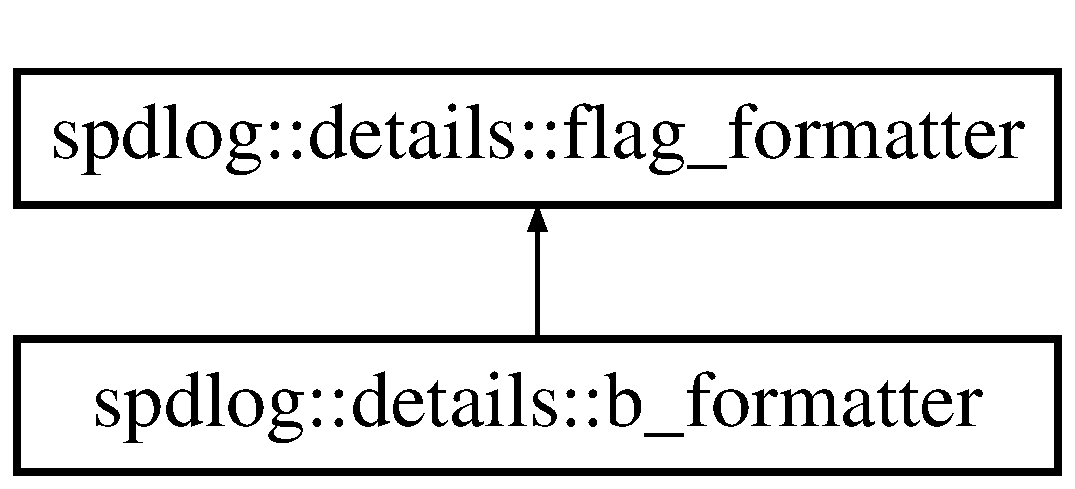
\includegraphics[height=2.000000cm]{classspdlog_1_1details_1_1b__formatter}
\end{center}
\end{figure}
\subsection*{Additional Inherited Members}


The documentation for this class was generated from the following file\+:\begin{DoxyCompactItemize}
\item 
cvdi-\/src/cvdi-\/cl/include/spdlog/details/pattern\+\_\+formatter\+\_\+impl.\+h\end{DoxyCompactItemize}

\hypertarget{classspdlog_1_1sinks_1_1base__sink}{}\section{spdlog\+:\+:sinks\+:\+:base\+\_\+sink$<$ Mutex $>$ Class Template Reference}
\label{classspdlog_1_1sinks_1_1base__sink}\index{spdlog\+::sinks\+::base\+\_\+sink$<$ Mutex $>$@{spdlog\+::sinks\+::base\+\_\+sink$<$ Mutex $>$}}
Inheritance diagram for spdlog\+:\+:sinks\+:\+:base\+\_\+sink$<$ Mutex $>$\+:\begin{figure}[H]
\begin{center}
\leavevmode
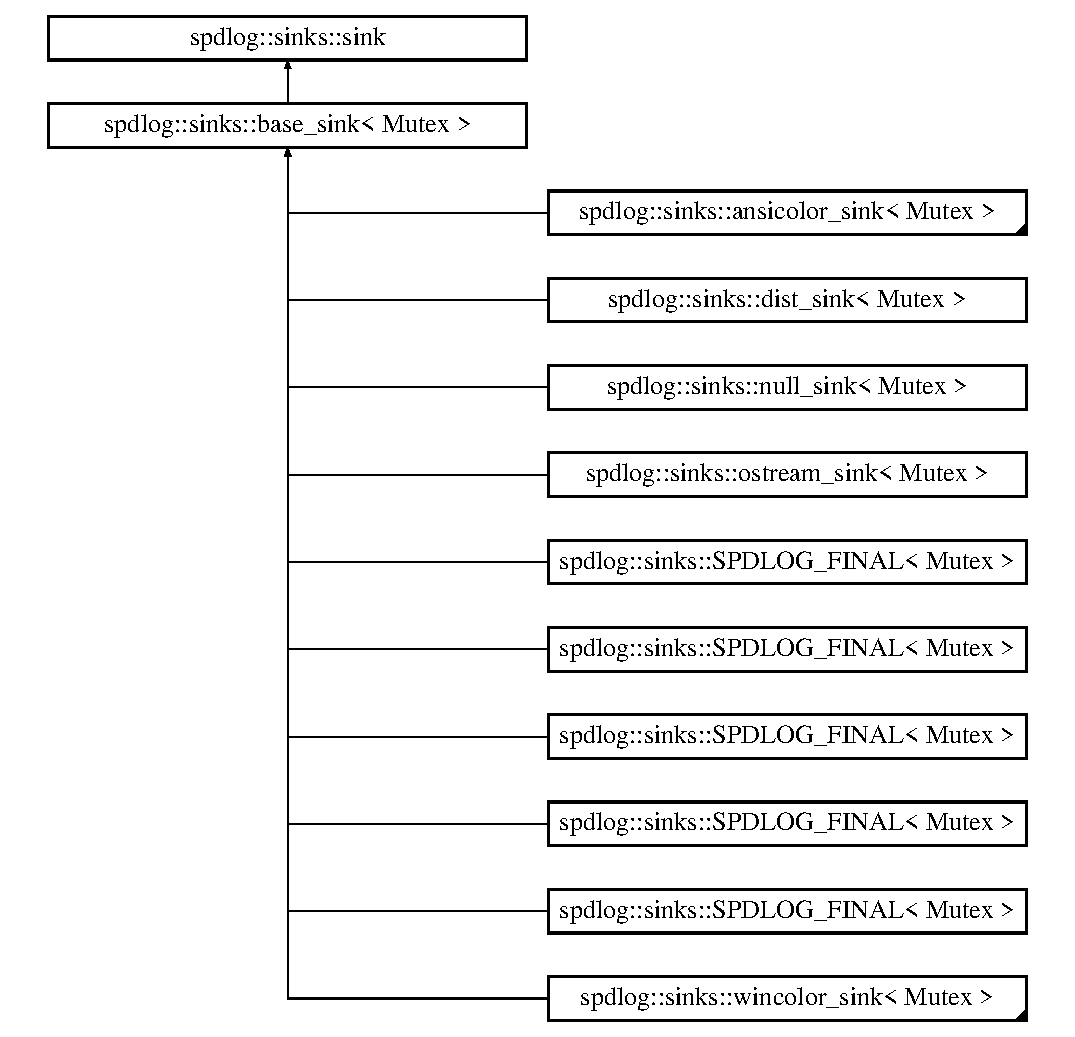
\includegraphics[height=12.000000cm]{classspdlog_1_1sinks_1_1base__sink}
\end{center}
\end{figure}
\subsection*{Public Member Functions}
\begin{DoxyCompactItemize}
\item 
{\bfseries base\+\_\+sink} (const \hyperlink{classspdlog_1_1sinks_1_1base__sink}{base\+\_\+sink} \&)=delete\hypertarget{classspdlog_1_1sinks_1_1base__sink_a9639062f2ce3598203c0d958576491d1}{}\label{classspdlog_1_1sinks_1_1base__sink_a9639062f2ce3598203c0d958576491d1}

\item 
\hyperlink{classspdlog_1_1sinks_1_1base__sink}{base\+\_\+sink} \& {\bfseries operator=} (const \hyperlink{classspdlog_1_1sinks_1_1base__sink}{base\+\_\+sink} \&)=delete\hypertarget{classspdlog_1_1sinks_1_1base__sink_a1b99823aeb2513a891bba168639421a9}{}\label{classspdlog_1_1sinks_1_1base__sink_a1b99823aeb2513a891bba168639421a9}

\item 
void {\bfseries log} (const \hyperlink{structspdlog_1_1details_1_1log__msg}{details\+::log\+\_\+msg} \&msg) \hyperlink{classspdlog_1_1sinks_1_1SPDLOG__FINAL}{S\+P\+D\+L\+O\+G\+\_\+\+F\+I\+N\+AL} override\hypertarget{classspdlog_1_1sinks_1_1base__sink_a2f435e651390945c4dd35df148b1a5eb}{}\label{classspdlog_1_1sinks_1_1base__sink_a2f435e651390945c4dd35df148b1a5eb}

\item 
void {\bfseries flush} () \hyperlink{classspdlog_1_1sinks_1_1SPDLOG__FINAL}{S\+P\+D\+L\+O\+G\+\_\+\+F\+I\+N\+AL} override\hypertarget{classspdlog_1_1sinks_1_1base__sink_a546c8690d7dadcba0bd716fc2d767a0b}{}\label{classspdlog_1_1sinks_1_1base__sink_a546c8690d7dadcba0bd716fc2d767a0b}

\end{DoxyCompactItemize}
\subsection*{Protected Member Functions}
\begin{DoxyCompactItemize}
\item 
virtual void {\bfseries \+\_\+sink\+\_\+it} (const \hyperlink{structspdlog_1_1details_1_1log__msg}{details\+::log\+\_\+msg} \&msg)=0\hypertarget{classspdlog_1_1sinks_1_1base__sink_a7a81101ba8dc0e19c77587c2a1e602ea}{}\label{classspdlog_1_1sinks_1_1base__sink_a7a81101ba8dc0e19c77587c2a1e602ea}

\item 
virtual void {\bfseries \+\_\+flush} ()=0\hypertarget{classspdlog_1_1sinks_1_1base__sink_a042217f781473c1f5a55d61dde6f2565}{}\label{classspdlog_1_1sinks_1_1base__sink_a042217f781473c1f5a55d61dde6f2565}

\end{DoxyCompactItemize}
\subsection*{Protected Attributes}
\begin{DoxyCompactItemize}
\item 
Mutex {\bfseries \+\_\+mutex}\hypertarget{classspdlog_1_1sinks_1_1base__sink_a1b380f67a77db4c384f9d02d7671e8a0}{}\label{classspdlog_1_1sinks_1_1base__sink_a1b380f67a77db4c384f9d02d7671e8a0}

\end{DoxyCompactItemize}


The documentation for this class was generated from the following file\+:\begin{DoxyCompactItemize}
\item 
cvdi-\/src/cvdi-\/cl/include/spdlog/sinks/base\+\_\+sink.\+h\end{DoxyCompactItemize}

\hypertarget{classfmt_1_1BasicArgFormatter}{}\section{fmt\+:\+:Basic\+Arg\+Formatter$<$ Impl, Char $>$ Class Template Reference}
\label{classfmt_1_1BasicArgFormatter}\index{fmt\+::\+Basic\+Arg\+Formatter$<$ Impl, Char $>$@{fmt\+::\+Basic\+Arg\+Formatter$<$ Impl, Char $>$}}


{\ttfamily \#include $<$format.\+h$>$}

Inheritance diagram for fmt\+:\+:Basic\+Arg\+Formatter$<$ Impl, Char $>$\+:\begin{figure}[H]
\begin{center}
\leavevmode
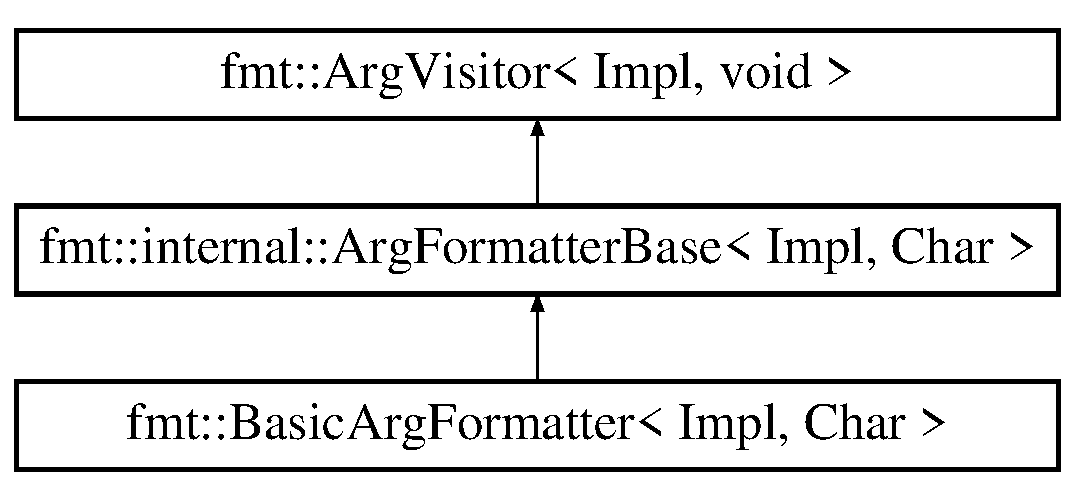
\includegraphics[height=3.000000cm]{classfmt_1_1BasicArgFormatter}
\end{center}
\end{figure}
\subsection*{Public Member Functions}
\begin{DoxyCompactItemize}
\item 
\hyperlink{classfmt_1_1BasicArgFormatter_a207b17b258c5e16cf61ebfc9b13211d3}{Basic\+Arg\+Formatter} (\hyperlink{classfmt_1_1BasicFormatter}{Basic\+Formatter}$<$ Char, Impl $>$ \&formatter, \hyperlink{structfmt_1_1FormatSpec}{Format\+Spec} \&spec, const Char $\ast$fmt)
\item 
void \hyperlink{classfmt_1_1BasicArgFormatter_ae0aab0f90c9c93e3513203fc84c2c4dc}{visit\+\_\+custom} (\hyperlink{structfmt_1_1internal_1_1Value_1_1CustomValue}{internal\+::\+Arg\+::\+Custom\+Value} c)
\end{DoxyCompactItemize}
\subsection*{Additional Inherited Members}


\subsection{Detailed Description}
\subsubsection*{template$<$typename Impl, typename Char$>$\\*
class fmt\+::\+Basic\+Arg\+Formatter$<$ Impl, Char $>$}

An argument formatter based on the {\ttfamily curiously recurring template pattern $<$\href{http://en.wikipedia.org/wiki/Curiously_recurring_template_pattern}{\tt http\+://en.\+wikipedia.\+org/wiki/\+Curiously\+\_\+recurring\+\_\+template\+\_\+pattern}$>$}\+\_\+.

To use {\ttfamily $\sim$fmt\+::\+Basic\+Arg\+Formatter} define a subclass that implements some or all of the visit methods with the same signatures as the methods in {\ttfamily $\sim$fmt\+::\+Arg\+Visitor}, for example, {\ttfamily $\sim$fmt\+::\+Arg\+Visitor\+::visit\+\_\+int()}. Pass the subclass as the {\itshape Impl} template parameter. When a formatting function processes an argument, it will dispatch to a visit method specific to the argument type. For example, if the argument type is {\ttfamily double} then the {\ttfamily $\sim$fmt\+::\+Arg\+Visitor\+::visit\+\_\+double()} method of a subclass will be called. If the subclass doesn\textquotesingle{}t contain a method with this signature, then a corresponding method of {\ttfamily $\sim$fmt\+::\+Basic\+Arg\+Formatter} or its superclass will be called.  

\subsection{Constructor \& Destructor Documentation}
\index{fmt\+::\+Basic\+Arg\+Formatter@{fmt\+::\+Basic\+Arg\+Formatter}!Basic\+Arg\+Formatter@{Basic\+Arg\+Formatter}}
\index{Basic\+Arg\+Formatter@{Basic\+Arg\+Formatter}!fmt\+::\+Basic\+Arg\+Formatter@{fmt\+::\+Basic\+Arg\+Formatter}}
\subsubsection[{\texorpdfstring{Basic\+Arg\+Formatter(\+Basic\+Formatter$<$ Char, Impl $>$ \&formatter, Format\+Spec \&spec, const Char $\ast$fmt)}{BasicArgFormatter(BasicFormatter< Char, Impl > &formatter, FormatSpec &spec, const Char *fmt)}}]{\setlength{\rightskip}{0pt plus 5cm}template$<$typename Impl, typename Char$>$ {\bf fmt\+::\+Basic\+Arg\+Formatter}$<$ Impl, Char $>$\+::{\bf Basic\+Arg\+Formatter} (
\begin{DoxyParamCaption}
\item[{{\bf Basic\+Formatter}$<$ Char, Impl $>$ \&}]{formatter, }
\item[{{\bf Format\+Spec} \&}]{spec, }
\item[{const Char $\ast$}]{fmt}
\end{DoxyParamCaption}
)\hspace{0.3cm}{\ttfamily [inline]}}\hypertarget{classfmt_1_1BasicArgFormatter_a207b17b258c5e16cf61ebfc9b13211d3}{}\label{classfmt_1_1BasicArgFormatter_a207b17b258c5e16cf61ebfc9b13211d3}
Constructs an argument formatter object. formatter$\ast$ is a reference to the main formatter object, {\itshape spec} contains format specifier information for standard argument types, and {\itshape fmt} points to the part of the format string being parsed for custom argument types.  

\subsection{Member Function Documentation}
\index{fmt\+::\+Basic\+Arg\+Formatter@{fmt\+::\+Basic\+Arg\+Formatter}!visit\+\_\+custom@{visit\+\_\+custom}}
\index{visit\+\_\+custom@{visit\+\_\+custom}!fmt\+::\+Basic\+Arg\+Formatter@{fmt\+::\+Basic\+Arg\+Formatter}}
\subsubsection[{\texorpdfstring{visit\+\_\+custom(internal\+::\+Arg\+::\+Custom\+Value c)}{visit_custom(internal::Arg::CustomValue c)}}]{\setlength{\rightskip}{0pt plus 5cm}template$<$typename Impl, typename Char$>$ void {\bf fmt\+::\+Basic\+Arg\+Formatter}$<$ Impl, Char $>$\+::visit\+\_\+custom (
\begin{DoxyParamCaption}
\item[{{\bf internal\+::\+Arg\+::\+Custom\+Value}}]{c}
\end{DoxyParamCaption}
)\hspace{0.3cm}{\ttfamily [inline]}}\hypertarget{classfmt_1_1BasicArgFormatter_ae0aab0f90c9c93e3513203fc84c2c4dc}{}\label{classfmt_1_1BasicArgFormatter_ae0aab0f90c9c93e3513203fc84c2c4dc}
Formats argument of a custom (user-\/defined) type. 

The documentation for this class was generated from the following file\+:\begin{DoxyCompactItemize}
\item 
cvdi-\/src/cvdi-\/cl/include/spdlog/fmt/bundled/format.\+h\end{DoxyCompactItemize}

\hypertarget{classfmt_1_1BasicArrayWriter}{}\section{fmt\+:\+:Basic\+Array\+Writer$<$ Char $>$ Class Template Reference}
\label{classfmt_1_1BasicArrayWriter}\index{fmt\+::\+Basic\+Array\+Writer$<$ Char $>$@{fmt\+::\+Basic\+Array\+Writer$<$ Char $>$}}


{\ttfamily \#include $<$format.\+h$>$}

Inheritance diagram for fmt\+:\+:Basic\+Array\+Writer$<$ Char $>$\+:\begin{figure}[H]
\begin{center}
\leavevmode
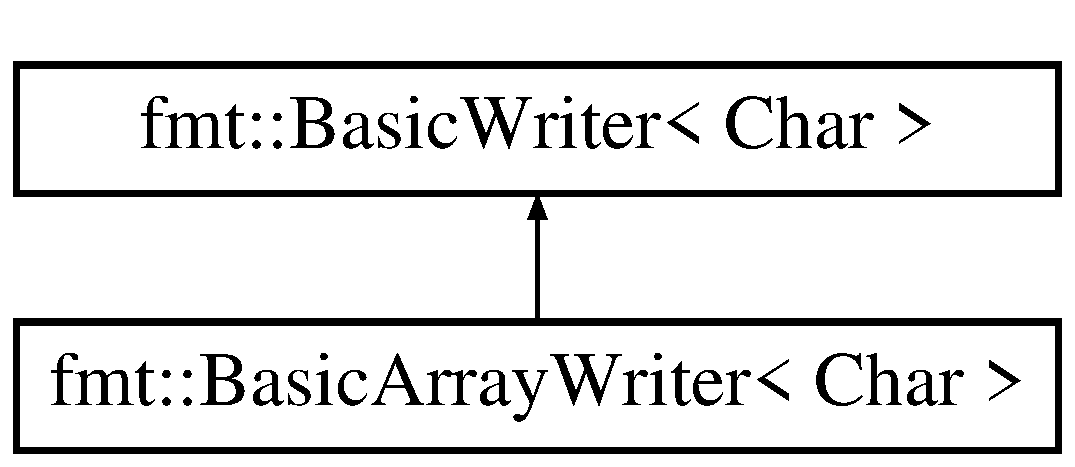
\includegraphics[height=2.000000cm]{classfmt_1_1BasicArrayWriter}
\end{center}
\end{figure}
\subsection*{Public Member Functions}
\begin{DoxyCompactItemize}
\item 
\hyperlink{classfmt_1_1BasicArrayWriter_a7559ecce2ffb3ecbb275dac5d2cc05e9}{Basic\+Array\+Writer} (Char $\ast$array, std\+::size\+\_\+t \hyperlink{classfmt_1_1BasicWriter_a1b6721b4ba4d3fa18ac781a36616cc2a}{size})
\item 
{\footnotesize template$<$std\+::size\+\_\+t S\+I\+ZE$>$ }\\\hyperlink{classfmt_1_1BasicArrayWriter_ab8787cfc9b1500c0f2765074f64e5088}{Basic\+Array\+Writer} (Char(\&array)\mbox{[}S\+I\+ZE\mbox{]})
\end{DoxyCompactItemize}
\subsection*{Additional Inherited Members}


\subsection{Detailed Description}
\subsubsection*{template$<$typename Char$>$\\*
class fmt\+::\+Basic\+Array\+Writer$<$ Char $>$}

This class template provides operations for formatting and writing data into a fixed-\/size array. For writing into a dynamically growing buffer use \+:class\+:{\ttfamily \hyperlink{classfmt_1_1BasicMemoryWriter}{fmt\+::\+Basic\+Memory\+Writer}}.

Any write method will throw {\ttfamily std\+::runtime\+\_\+error} if the output doesn\textquotesingle{}t fit into the array.

You can use one of the following typedefs for common character types\+:

+-\/-\/-\/-\/-\/-\/-\/-\/-\/-\/-\/---+-\/-\/-\/-\/-\/-\/-\/-\/-\/-\/-\/-\/-\/-\/-\/-\/-\/-\/-\/-\/-\/-\/-\/-\/---+ $\vert$ Type $\vert$ Definition $\vert$ +==============+===========================+ $\vert$ Array\+Writer $\vert$ Basic\+Array\+Writer$<$char$>$ $\vert$ +-\/-\/-\/-\/-\/-\/-\/-\/-\/-\/-\/---+-\/-\/-\/-\/-\/-\/-\/-\/-\/-\/-\/-\/-\/-\/-\/-\/-\/-\/-\/-\/-\/-\/-\/-\/---+ $\vert$ W\+Array\+Writer $\vert$ Basic\+Array\+Writer$<$wchar\+\_\+t$>$ $\vert$ +-\/-\/-\/-\/-\/-\/-\/-\/-\/-\/-\/---+-\/-\/-\/-\/-\/-\/-\/-\/-\/-\/-\/-\/-\/-\/-\/-\/-\/-\/-\/-\/-\/-\/-\/-\/---+  

\subsection{Constructor \& Destructor Documentation}
\index{fmt\+::\+Basic\+Array\+Writer@{fmt\+::\+Basic\+Array\+Writer}!Basic\+Array\+Writer@{Basic\+Array\+Writer}}
\index{Basic\+Array\+Writer@{Basic\+Array\+Writer}!fmt\+::\+Basic\+Array\+Writer@{fmt\+::\+Basic\+Array\+Writer}}
\subsubsection[{\texorpdfstring{Basic\+Array\+Writer(\+Char $\ast$array, std\+::size\+\_\+t size)}{BasicArrayWriter(Char *array, std::size_t size)}}]{\setlength{\rightskip}{0pt plus 5cm}template$<$typename Char $>$ {\bf fmt\+::\+Basic\+Array\+Writer}$<$ Char $>$\+::{\bf Basic\+Array\+Writer} (
\begin{DoxyParamCaption}
\item[{Char $\ast$}]{array, }
\item[{std\+::size\+\_\+t}]{size}
\end{DoxyParamCaption}
)\hspace{0.3cm}{\ttfamily [inline]}}\hypertarget{classfmt_1_1BasicArrayWriter_a7559ecce2ffb3ecbb275dac5d2cc05e9}{}\label{classfmt_1_1BasicArrayWriter_a7559ecce2ffb3ecbb275dac5d2cc05e9}
Constructs a \+:class\+:{\ttfamily \hyperlink{classfmt_1_1BasicArrayWriter}{fmt\+::\+Basic\+Array\+Writer}} object for {\itshape array} of the given size.  \index{fmt\+::\+Basic\+Array\+Writer@{fmt\+::\+Basic\+Array\+Writer}!Basic\+Array\+Writer@{Basic\+Array\+Writer}}
\index{Basic\+Array\+Writer@{Basic\+Array\+Writer}!fmt\+::\+Basic\+Array\+Writer@{fmt\+::\+Basic\+Array\+Writer}}
\subsubsection[{\texorpdfstring{Basic\+Array\+Writer(\+Char(\&array)[S\+I\+ZE])}{BasicArrayWriter(Char(&array)[SIZE])}}]{\setlength{\rightskip}{0pt plus 5cm}template$<$typename Char $>$ template$<$std\+::size\+\_\+t S\+I\+ZE$>$ {\bf fmt\+::\+Basic\+Array\+Writer}$<$ Char $>$\+::{\bf Basic\+Array\+Writer} (
\begin{DoxyParamCaption}
\item[{Char(\&)}]{array\mbox{[}\+S\+I\+Z\+E\mbox{]}}
\end{DoxyParamCaption}
)\hspace{0.3cm}{\ttfamily [inline]}, {\ttfamily [explicit]}}\hypertarget{classfmt_1_1BasicArrayWriter_ab8787cfc9b1500c0f2765074f64e5088}{}\label{classfmt_1_1BasicArrayWriter_ab8787cfc9b1500c0f2765074f64e5088}
Constructs a \+:class\+:{\ttfamily \hyperlink{classfmt_1_1BasicArrayWriter}{fmt\+::\+Basic\+Array\+Writer}} object for {\itshape array} of the size known at compile time.  

The documentation for this class was generated from the following file\+:\begin{DoxyCompactItemize}
\item 
cvdi-\/src/cvdi-\/cl/include/spdlog/fmt/bundled/format.\+h\end{DoxyCompactItemize}

\hypertarget{classfmt_1_1internal_1_1BasicCharTraits}{}\section{fmt\+:\+:internal\+:\+:Basic\+Char\+Traits$<$ Char $>$ Class Template Reference}
\label{classfmt_1_1internal_1_1BasicCharTraits}\index{fmt\+::internal\+::\+Basic\+Char\+Traits$<$ Char $>$@{fmt\+::internal\+::\+Basic\+Char\+Traits$<$ Char $>$}}
\subsection*{Public Types}
\begin{DoxyCompactItemize}
\item 
typedef Char $\ast$ {\bfseries Char\+Ptr}\hypertarget{classfmt_1_1internal_1_1BasicCharTraits_a32f5cad709328e0450b8690960d6b8b5}{}\label{classfmt_1_1internal_1_1BasicCharTraits_a32f5cad709328e0450b8690960d6b8b5}

\end{DoxyCompactItemize}
\subsection*{Static Public Member Functions}
\begin{DoxyCompactItemize}
\item 
static Char {\bfseries cast} (int value)\hypertarget{classfmt_1_1internal_1_1BasicCharTraits_a5ec7e07adb183b9bf1e63a7507382ec6}{}\label{classfmt_1_1internal_1_1BasicCharTraits_a5ec7e07adb183b9bf1e63a7507382ec6}

\end{DoxyCompactItemize}


The documentation for this class was generated from the following file\+:\begin{DoxyCompactItemize}
\item 
cvdi-\/src/cvdi-\/cl/include/spdlog/fmt/bundled/format.\+h\end{DoxyCompactItemize}

\hypertarget{classfmt_1_1BasicCStringRef}{}\section{fmt\+:\+:Basic\+C\+String\+Ref$<$ Char $>$ Class Template Reference}
\label{classfmt_1_1BasicCStringRef}\index{fmt\+::\+Basic\+C\+String\+Ref$<$ Char $>$@{fmt\+::\+Basic\+C\+String\+Ref$<$ Char $>$}}


{\ttfamily \#include $<$format.\+h$>$}

\subsection*{Public Member Functions}
\begin{DoxyCompactItemize}
\item 
\hyperlink{classfmt_1_1BasicCStringRef_ad79244507bdc1213e0dc6c505cf265f2}{Basic\+C\+String\+Ref} (const Char $\ast$s)
\item 
\hyperlink{classfmt_1_1BasicCStringRef_ab460855d19c769773de532296f9f13f9}{Basic\+C\+String\+Ref} (const std\+::basic\+\_\+string$<$ Char $>$ \&s)
\item 
const Char $\ast$ \hyperlink{classfmt_1_1BasicCStringRef_ae3bafa845b53339b20c4f5edb4f635f9}{c\+\_\+str} () const 
\end{DoxyCompactItemize}


\subsection{Detailed Description}
\subsubsection*{template$<$typename Char$>$\\*
class fmt\+::\+Basic\+C\+String\+Ref$<$ Char $>$}

A reference to a null terminated string. It can be constructed from a C string or {\ttfamily std\+::string}.

You can use one of the following typedefs for common character types\+:

+-\/-\/-\/-\/-\/-\/-\/-\/-\/-\/---+-\/-\/-\/-\/-\/-\/-\/-\/-\/-\/-\/-\/-\/-\/-\/-\/-\/-\/-\/-\/-\/-\/-\/---+ $\vert$ Type $\vert$ Definition $\vert$ +=============+==========================+ $\vert$ C\+String\+Ref $\vert$ Basic\+C\+String\+Ref$<$char$>$ $\vert$ +-\/-\/-\/-\/-\/-\/-\/-\/-\/-\/---+-\/-\/-\/-\/-\/-\/-\/-\/-\/-\/-\/-\/-\/-\/-\/-\/-\/-\/-\/-\/-\/-\/-\/---+ $\vert$ W\+C\+String\+Ref $\vert$ Basic\+C\+String\+Ref$<$wchar\+\_\+t$>$ $\vert$ +-\/-\/-\/-\/-\/-\/-\/-\/-\/-\/---+-\/-\/-\/-\/-\/-\/-\/-\/-\/-\/-\/-\/-\/-\/-\/-\/-\/-\/-\/-\/-\/-\/-\/---+

This class is most useful as a parameter type to allow passing different types of strings to a function, for example\+:\+:

template $<$typename... Args$>$ std\+::string format(C\+String\+Ref format\+\_\+str, const Args \& ... args);

format(\char`\"{}\{\}\char`\"{}, 42); format(std\+::string(\char`\"{}\{\}\char`\"{}), 42);  

\subsection{Constructor \& Destructor Documentation}
\index{fmt\+::\+Basic\+C\+String\+Ref@{fmt\+::\+Basic\+C\+String\+Ref}!Basic\+C\+String\+Ref@{Basic\+C\+String\+Ref}}
\index{Basic\+C\+String\+Ref@{Basic\+C\+String\+Ref}!fmt\+::\+Basic\+C\+String\+Ref@{fmt\+::\+Basic\+C\+String\+Ref}}
\subsubsection[{\texorpdfstring{Basic\+C\+String\+Ref(const Char $\ast$s)}{BasicCStringRef(const Char *s)}}]{\setlength{\rightskip}{0pt plus 5cm}template$<$typename Char$>$ {\bf fmt\+::\+Basic\+C\+String\+Ref}$<$ Char $>$\+::{\bf Basic\+C\+String\+Ref} (
\begin{DoxyParamCaption}
\item[{const Char $\ast$}]{s}
\end{DoxyParamCaption}
)\hspace{0.3cm}{\ttfamily [inline]}}\hypertarget{classfmt_1_1BasicCStringRef_ad79244507bdc1213e0dc6c505cf265f2}{}\label{classfmt_1_1BasicCStringRef_ad79244507bdc1213e0dc6c505cf265f2}
Constructs a string reference object from a C string. \index{fmt\+::\+Basic\+C\+String\+Ref@{fmt\+::\+Basic\+C\+String\+Ref}!Basic\+C\+String\+Ref@{Basic\+C\+String\+Ref}}
\index{Basic\+C\+String\+Ref@{Basic\+C\+String\+Ref}!fmt\+::\+Basic\+C\+String\+Ref@{fmt\+::\+Basic\+C\+String\+Ref}}
\subsubsection[{\texorpdfstring{Basic\+C\+String\+Ref(const std\+::basic\+\_\+string$<$ Char $>$ \&s)}{BasicCStringRef(const std::basic_string< Char > &s)}}]{\setlength{\rightskip}{0pt plus 5cm}template$<$typename Char$>$ {\bf fmt\+::\+Basic\+C\+String\+Ref}$<$ Char $>$\+::{\bf Basic\+C\+String\+Ref} (
\begin{DoxyParamCaption}
\item[{const std\+::basic\+\_\+string$<$ Char $>$ \&}]{s}
\end{DoxyParamCaption}
)\hspace{0.3cm}{\ttfamily [inline]}}\hypertarget{classfmt_1_1BasicCStringRef_ab460855d19c769773de532296f9f13f9}{}\label{classfmt_1_1BasicCStringRef_ab460855d19c769773de532296f9f13f9}
Constructs a string reference from an {\ttfamily std\+::string} object.  

\subsection{Member Function Documentation}
\index{fmt\+::\+Basic\+C\+String\+Ref@{fmt\+::\+Basic\+C\+String\+Ref}!c\+\_\+str@{c\+\_\+str}}
\index{c\+\_\+str@{c\+\_\+str}!fmt\+::\+Basic\+C\+String\+Ref@{fmt\+::\+Basic\+C\+String\+Ref}}
\subsubsection[{\texorpdfstring{c\+\_\+str() const }{c_str() const }}]{\setlength{\rightskip}{0pt plus 5cm}template$<$typename Char$>$ const Char$\ast$ {\bf fmt\+::\+Basic\+C\+String\+Ref}$<$ Char $>$\+::c\+\_\+str (
\begin{DoxyParamCaption}
{}
\end{DoxyParamCaption}
) const\hspace{0.3cm}{\ttfamily [inline]}}\hypertarget{classfmt_1_1BasicCStringRef_ae3bafa845b53339b20c4f5edb4f635f9}{}\label{classfmt_1_1BasicCStringRef_ae3bafa845b53339b20c4f5edb4f635f9}
Returns the pointer to a C string. 

The documentation for this class was generated from the following file\+:\begin{DoxyCompactItemize}
\item 
cvdi-\/src/cvdi-\/cl/include/spdlog/fmt/bundled/format.\+h\end{DoxyCompactItemize}

\hypertarget{structfmt_1_1internal_1_1BasicData}{}\section{fmt\+:\+:internal\+:\+:Basic\+Data$<$ T $>$ Struct Template Reference}
\label{structfmt_1_1internal_1_1BasicData}\index{fmt\+::internal\+::\+Basic\+Data$<$ T $>$@{fmt\+::internal\+::\+Basic\+Data$<$ T $>$}}
\subsection*{Static Public Attributes}
\begin{DoxyCompactItemize}
\item 
static const uint32\+\_\+t {\bfseries P\+O\+W\+E\+R\+S\+\_\+\+O\+F\+\_\+10\+\_\+32} \mbox{[}$\,$\mbox{]}
\item 
static const uint64\+\_\+t {\bfseries P\+O\+W\+E\+R\+S\+\_\+\+O\+F\+\_\+10\+\_\+64} \mbox{[}$\,$\mbox{]}
\item 
static const char {\bfseries D\+I\+G\+I\+TS} \mbox{[}$\,$\mbox{]}
\end{DoxyCompactItemize}


\subsection{Member Data Documentation}
\index{fmt\+::internal\+::\+Basic\+Data@{fmt\+::internal\+::\+Basic\+Data}!D\+I\+G\+I\+TS@{D\+I\+G\+I\+TS}}
\index{D\+I\+G\+I\+TS@{D\+I\+G\+I\+TS}!fmt\+::internal\+::\+Basic\+Data@{fmt\+::internal\+::\+Basic\+Data}}
\subsubsection[{\texorpdfstring{D\+I\+G\+I\+TS}{DIGITS}}]{\setlength{\rightskip}{0pt plus 5cm}template$<$typename T  = void$>$ const char {\bf fmt\+::internal\+::\+Basic\+Data}$<$ T $>$\+::D\+I\+G\+I\+TS\hspace{0.3cm}{\ttfamily [static]}}\hypertarget{structfmt_1_1internal_1_1BasicData_abc0f1b67b25a98d0aa1f2b25c8649e59}{}\label{structfmt_1_1internal_1_1BasicData_abc0f1b67b25a98d0aa1f2b25c8649e59}
{\bfseries Initial value\+:}
\begin{DoxyCode}
=
    \textcolor{stringliteral}{"0001020304050607080910111213141516171819"}
    \textcolor{stringliteral}{"2021222324252627282930313233343536373839"}
    \textcolor{stringliteral}{"4041424344454647484950515253545556575859"}
    \textcolor{stringliteral}{"6061626364656667686970717273747576777879"}
    \textcolor{stringliteral}{"8081828384858687888990919293949596979899"}
\end{DoxyCode}
\index{fmt\+::internal\+::\+Basic\+Data@{fmt\+::internal\+::\+Basic\+Data}!P\+O\+W\+E\+R\+S\+\_\+\+O\+F\+\_\+10\+\_\+32@{P\+O\+W\+E\+R\+S\+\_\+\+O\+F\+\_\+10\+\_\+32}}
\index{P\+O\+W\+E\+R\+S\+\_\+\+O\+F\+\_\+10\+\_\+32@{P\+O\+W\+E\+R\+S\+\_\+\+O\+F\+\_\+10\+\_\+32}!fmt\+::internal\+::\+Basic\+Data@{fmt\+::internal\+::\+Basic\+Data}}
\subsubsection[{\texorpdfstring{P\+O\+W\+E\+R\+S\+\_\+\+O\+F\+\_\+10\+\_\+32}{POWERS_OF_10_32}}]{\setlength{\rightskip}{0pt plus 5cm}template$<$typename T  = void$>$ const uint32\+\_\+t {\bf fmt\+::internal\+::\+Basic\+Data}$<$ T $>$\+::P\+O\+W\+E\+R\+S\+\_\+\+O\+F\+\_\+10\+\_\+32\hspace{0.3cm}{\ttfamily [static]}}\hypertarget{structfmt_1_1internal_1_1BasicData_abbc4c0076211263be3f19cce9655caf7}{}\label{structfmt_1_1internal_1_1BasicData_abbc4c0076211263be3f19cce9655caf7}
{\bfseries Initial value\+:}
\begin{DoxyCode}
= \{
  0, FMT\_POWERS\_OF\_10(1)
\}
\end{DoxyCode}
\index{fmt\+::internal\+::\+Basic\+Data@{fmt\+::internal\+::\+Basic\+Data}!P\+O\+W\+E\+R\+S\+\_\+\+O\+F\+\_\+10\+\_\+64@{P\+O\+W\+E\+R\+S\+\_\+\+O\+F\+\_\+10\+\_\+64}}
\index{P\+O\+W\+E\+R\+S\+\_\+\+O\+F\+\_\+10\+\_\+64@{P\+O\+W\+E\+R\+S\+\_\+\+O\+F\+\_\+10\+\_\+64}!fmt\+::internal\+::\+Basic\+Data@{fmt\+::internal\+::\+Basic\+Data}}
\subsubsection[{\texorpdfstring{P\+O\+W\+E\+R\+S\+\_\+\+O\+F\+\_\+10\+\_\+64}{POWERS_OF_10_64}}]{\setlength{\rightskip}{0pt plus 5cm}template$<$typename T  = void$>$ const uint64\+\_\+t {\bf fmt\+::internal\+::\+Basic\+Data}$<$ T $>$\+::P\+O\+W\+E\+R\+S\+\_\+\+O\+F\+\_\+10\+\_\+64\hspace{0.3cm}{\ttfamily [static]}}\hypertarget{structfmt_1_1internal_1_1BasicData_a5f4f238cffad6816fbdc621e96b0e1d2}{}\label{structfmt_1_1internal_1_1BasicData_a5f4f238cffad6816fbdc621e96b0e1d2}
{\bfseries Initial value\+:}
\begin{DoxyCode}
= \{
  0,
  FMT\_POWERS\_OF\_10(1),
  FMT\_POWERS\_OF\_10(fmt::ULongLong(1000000000)),
  
  
  fmt::ULongLong(1000000000) * fmt::ULongLong(1000000000) * 10
\}
\end{DoxyCode}


The documentation for this struct was generated from the following files\+:\begin{DoxyCompactItemize}
\item 
cvdi-\/src/cvdi-\/cl/include/spdlog/fmt/bundled/format.\+h\item 
cvdi-\/src/cvdi-\/cl/include/spdlog/fmt/bundled/format.\+cc\end{DoxyCompactItemize}

\hypertarget{classfmt_1_1BasicFormatter}{}\section{fmt\+:\+:Basic\+Formatter$<$ Char\+Type, Arg\+Formatter $>$ Class Template Reference}
\label{classfmt_1_1BasicFormatter}\index{fmt\+::\+Basic\+Formatter$<$ Char\+Type, Arg\+Formatter $>$@{fmt\+::\+Basic\+Formatter$<$ Char\+Type, Arg\+Formatter $>$}}


{\ttfamily \#include $<$format.\+h$>$}

Inheritance diagram for fmt\+:\+:Basic\+Formatter$<$ Char\+Type, Arg\+Formatter $>$\+:\begin{figure}[H]
\begin{center}
\leavevmode
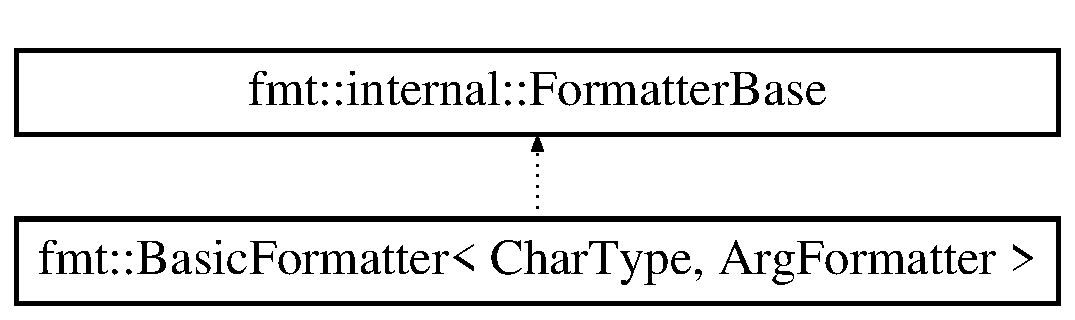
\includegraphics[height=2.000000cm]{classfmt_1_1BasicFormatter}
\end{center}
\end{figure}
\subsection*{Public Types}
\begin{DoxyCompactItemize}
\item 
typedef Char\+Type \hyperlink{classfmt_1_1BasicFormatter_af8270b25395aeb82b8c72c370c5cf13a}{Char}
\end{DoxyCompactItemize}
\subsection*{Public Member Functions}
\begin{DoxyCompactItemize}
\item 
\hyperlink{classfmt_1_1BasicFormatter_a2b190901681ff0413dc60522fe158fdc}{Basic\+Formatter} (const \hyperlink{classfmt_1_1ArgList}{Arg\+List} \&args, \hyperlink{classfmt_1_1BasicWriter}{Basic\+Writer}$<$ \hyperlink{classfmt_1_1BasicFormatter_af8270b25395aeb82b8c72c370c5cf13a}{Char} $>$ \&w)
\item 
\hyperlink{classfmt_1_1BasicWriter}{Basic\+Writer}$<$ \hyperlink{classfmt_1_1BasicFormatter_af8270b25395aeb82b8c72c370c5cf13a}{Char} $>$ \& \hyperlink{classfmt_1_1BasicFormatter_abd5692d2f2123b27da7941d56fc6073c}{writer} ()
\item 
void \hyperlink{classfmt_1_1BasicFormatter_a63acecbbf9681005f3c7eb4d42a54bf7}{format} (\hyperlink{classfmt_1_1BasicCStringRef}{Basic\+C\+String\+Ref}$<$ \hyperlink{classfmt_1_1BasicFormatter_af8270b25395aeb82b8c72c370c5cf13a}{Char} $>$ format\+\_\+str)
\item 
const \hyperlink{classfmt_1_1BasicFormatter_af8270b25395aeb82b8c72c370c5cf13a}{Char} $\ast$ {\bfseries format} (const \hyperlink{classfmt_1_1BasicFormatter_af8270b25395aeb82b8c72c370c5cf13a}{Char} $\ast$\&format\+\_\+str, const \hyperlink{structfmt_1_1internal_1_1Arg}{internal\+::\+Arg} \&arg)\hypertarget{classfmt_1_1BasicFormatter_ab436d449f9a0678badb672af2a8ecb32}{}\label{classfmt_1_1BasicFormatter_ab436d449f9a0678badb672af2a8ecb32}

\end{DoxyCompactItemize}


\subsection{Detailed Description}
\subsubsection*{template$<$typename Char\+Type, typename Arg\+Formatter$>$\\*
class fmt\+::\+Basic\+Formatter$<$ Char\+Type, Arg\+Formatter $>$}

This template formats data and writes the output to a writer. 

\subsection{Member Typedef Documentation}
\index{fmt\+::\+Basic\+Formatter@{fmt\+::\+Basic\+Formatter}!Char@{Char}}
\index{Char@{Char}!fmt\+::\+Basic\+Formatter@{fmt\+::\+Basic\+Formatter}}
\subsubsection[{\texorpdfstring{Char}{Char}}]{\setlength{\rightskip}{0pt plus 5cm}template$<$typename Char\+Type, typename Arg\+Formatter$>$ typedef Char\+Type {\bf fmt\+::\+Basic\+Formatter}$<$ Char\+Type, {\bf Arg\+Formatter} $>$\+::{\bf Char}}\hypertarget{classfmt_1_1BasicFormatter_af8270b25395aeb82b8c72c370c5cf13a}{}\label{classfmt_1_1BasicFormatter_af8270b25395aeb82b8c72c370c5cf13a}
The character type for the output. 

\subsection{Constructor \& Destructor Documentation}
\index{fmt\+::\+Basic\+Formatter@{fmt\+::\+Basic\+Formatter}!Basic\+Formatter@{Basic\+Formatter}}
\index{Basic\+Formatter@{Basic\+Formatter}!fmt\+::\+Basic\+Formatter@{fmt\+::\+Basic\+Formatter}}
\subsubsection[{\texorpdfstring{Basic\+Formatter(const Arg\+List \&args, Basic\+Writer$<$ Char $>$ \&w)}{BasicFormatter(const ArgList &args, BasicWriter< Char > &w)}}]{\setlength{\rightskip}{0pt plus 5cm}template$<$typename Char\+Type, typename Arg\+Formatter$>$ {\bf fmt\+::\+Basic\+Formatter}$<$ Char\+Type, {\bf Arg\+Formatter} $>$\+::{\bf Basic\+Formatter} (
\begin{DoxyParamCaption}
\item[{const {\bf Arg\+List} \&}]{args, }
\item[{{\bf Basic\+Writer}$<$ {\bf Char} $>$ \&}]{w}
\end{DoxyParamCaption}
)\hspace{0.3cm}{\ttfamily [inline]}}\hypertarget{classfmt_1_1BasicFormatter_a2b190901681ff0413dc60522fe158fdc}{}\label{classfmt_1_1BasicFormatter_a2b190901681ff0413dc60522fe158fdc}
Constructs a {\ttfamily \hyperlink{classfmt_1_1BasicFormatter}{Basic\+Formatter}} object. References to the arguments and the writer are stored in the formatter object so make sure they have appropriate lifetimes.  

\subsection{Member Function Documentation}
\index{fmt\+::\+Basic\+Formatter@{fmt\+::\+Basic\+Formatter}!format@{format}}
\index{format@{format}!fmt\+::\+Basic\+Formatter@{fmt\+::\+Basic\+Formatter}}
\subsubsection[{\texorpdfstring{format(\+Basic\+C\+String\+Ref$<$ Char $>$ format\+\_\+str)}{format(BasicCStringRef< Char > format_str)}}]{\setlength{\rightskip}{0pt plus 5cm}template$<$typename Char , typename AF $>$ void {\bf fmt\+::\+Basic\+Formatter}$<$ {\bf Char}, AF $>$\+::format (
\begin{DoxyParamCaption}
\item[{{\bf Basic\+C\+String\+Ref}$<$ {\bf Char} $>$}]{format\+\_\+str}
\end{DoxyParamCaption}
)}\hypertarget{classfmt_1_1BasicFormatter_a63acecbbf9681005f3c7eb4d42a54bf7}{}\label{classfmt_1_1BasicFormatter_a63acecbbf9681005f3c7eb4d42a54bf7}
Formats stored arguments and writes the output to the writer. \index{fmt\+::\+Basic\+Formatter@{fmt\+::\+Basic\+Formatter}!writer@{writer}}
\index{writer@{writer}!fmt\+::\+Basic\+Formatter@{fmt\+::\+Basic\+Formatter}}
\subsubsection[{\texorpdfstring{writer()}{writer()}}]{\setlength{\rightskip}{0pt plus 5cm}template$<$typename Char\+Type, typename Arg\+Formatter$>$ {\bf Basic\+Writer}$<${\bf Char}$>$\& {\bf fmt\+::\+Basic\+Formatter}$<$ Char\+Type, {\bf Arg\+Formatter} $>$\+::writer (
\begin{DoxyParamCaption}
{}
\end{DoxyParamCaption}
)\hspace{0.3cm}{\ttfamily [inline]}}\hypertarget{classfmt_1_1BasicFormatter_abd5692d2f2123b27da7941d56fc6073c}{}\label{classfmt_1_1BasicFormatter_abd5692d2f2123b27da7941d56fc6073c}
Returns a reference to the writer associated with this formatter. 

The documentation for this class was generated from the following file\+:\begin{DoxyCompactItemize}
\item 
cvdi-\/src/cvdi-\/cl/include/spdlog/fmt/bundled/format.\+h\end{DoxyCompactItemize}

\hypertarget{classfmt_1_1BasicMemoryWriter}{}\section{fmt\+:\+:Basic\+Memory\+Writer$<$ Char, Allocator $>$ Class Template Reference}
\label{classfmt_1_1BasicMemoryWriter}\index{fmt\+::\+Basic\+Memory\+Writer$<$ Char, Allocator $>$@{fmt\+::\+Basic\+Memory\+Writer$<$ Char, Allocator $>$}}


{\ttfamily \#include $<$format.\+h$>$}

Inheritance diagram for fmt\+:\+:Basic\+Memory\+Writer$<$ Char, Allocator $>$\+:\begin{figure}[H]
\begin{center}
\leavevmode
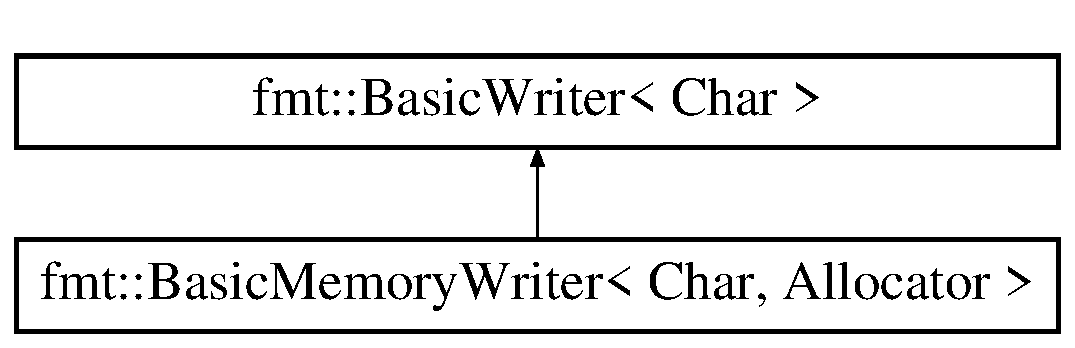
\includegraphics[height=2.000000cm]{classfmt_1_1BasicMemoryWriter}
\end{center}
\end{figure}
\subsection*{Public Member Functions}
\begin{DoxyCompactItemize}
\item 
{\bfseries Basic\+Memory\+Writer} (const Allocator \&alloc=Allocator())\hypertarget{classfmt_1_1BasicMemoryWriter_a36ef881adce8fc7a0b3632d2fb66fdfb}{}\label{classfmt_1_1BasicMemoryWriter_a36ef881adce8fc7a0b3632d2fb66fdfb}

\end{DoxyCompactItemize}
\subsection*{Additional Inherited Members}


\subsection{Detailed Description}
\subsubsection*{template$<$typename Char, typename Allocator = std\+::allocator$<$\+Char$>$$>$\\*
class fmt\+::\+Basic\+Memory\+Writer$<$ Char, Allocator $>$}

This class template provides operations for formatting and writing data into a character stream. The output is stored in a memory buffer that grows dynamically.

You can use one of the following typedefs for common character types and the standard allocator\+:

+-\/-\/-\/-\/-\/-\/-\/-\/-\/-\/-\/-\/---+-\/-\/-\/-\/-\/-\/-\/-\/-\/-\/-\/-\/-\/-\/-\/-\/-\/-\/-\/-\/-\/-\/-\/-\/-\/-\/-\/-\/-\/-\/-\/-\/-\/-\/-\/-\/-\/-\/-\/-\/-\/-\/-\/-\/-\/-\/-\/-\/-\/-\/---+ $\vert$ Type $\vert$ Definition $\vert$ +===============+=====================================================+ $\vert$ Memory\+Writer $\vert$ \hyperlink{classfmt_1_1BasicMemoryWriter}{Basic\+Memory\+Writer}$<$char, std\+::allocator$<$char$>$$>$ $\vert$ +-\/-\/-\/-\/-\/-\/-\/-\/-\/-\/-\/-\/---+-\/-\/-\/-\/-\/-\/-\/-\/-\/-\/-\/-\/-\/-\/-\/-\/-\/-\/-\/-\/-\/-\/-\/-\/-\/-\/-\/-\/-\/-\/-\/-\/-\/-\/-\/-\/-\/-\/-\/-\/-\/-\/-\/-\/-\/-\/-\/-\/-\/-\/---+ $\vert$ W\+Memory\+Writer $\vert$ \hyperlink{classfmt_1_1BasicMemoryWriter}{Basic\+Memory\+Writer}$<$wchar\+\_\+t, std\+::allocator$<$wchar\+\_\+t$>$$>$ $\vert$ +-\/-\/-\/-\/-\/-\/-\/-\/-\/-\/-\/-\/---+-\/-\/-\/-\/-\/-\/-\/-\/-\/-\/-\/-\/-\/-\/-\/-\/-\/-\/-\/-\/-\/-\/-\/-\/-\/-\/-\/-\/-\/-\/-\/-\/-\/-\/-\/-\/-\/-\/-\/-\/-\/-\/-\/-\/-\/-\/-\/-\/-\/-\/---+

Example$\ast$$\ast$\+:\+:

Memory\+Writer out; out $<$$<$ \char`\"{}\+The answer is \char`\"{} $<$$<$ 42 $<$$<$ \char`\"{}\textbackslash{}n\char`\"{}; out.\+write(\char`\"{}(\{\+:+f\}, \{\+:+f\})\char`\"{}, -\/3.\+14, 3.\+14);

This will write the following output to the {\ttfamily out} object\+:

.. code-\/block\+:\+: none

The answer is 42 (-\/3.\+140000, +3.140000)

The output can be converted to an {\ttfamily std\+::string} with {\ttfamily out.\+str()} or accessed as a C string with {\ttfamily out.\+c\+\_\+str()}.  

The documentation for this class was generated from the following file\+:\begin{DoxyCompactItemize}
\item 
cvdi-\/src/cvdi-\/cl/include/spdlog/fmt/bundled/format.\+h\end{DoxyCompactItemize}

\hypertarget{classfmt_1_1BasicStringRef}{}\section{fmt\+:\+:Basic\+String\+Ref$<$ Char $>$ Class Template Reference}
\label{classfmt_1_1BasicStringRef}\index{fmt\+::\+Basic\+String\+Ref$<$ Char $>$@{fmt\+::\+Basic\+String\+Ref$<$ Char $>$}}


{\ttfamily \#include $<$format.\+h$>$}

\subsection*{Public Member Functions}
\begin{DoxyCompactItemize}
\item 
\hyperlink{classfmt_1_1BasicStringRef_adc7198e4dbd3eefff16081aae819181a}{Basic\+String\+Ref} (const Char $\ast$s, std\+::size\+\_\+t \hyperlink{classfmt_1_1BasicStringRef_ae38d9106dd5bec69488e5464aedc266a}{size})
\item 
\hyperlink{classfmt_1_1BasicStringRef_a5e3875071c0be193aa706d6c8e7bf29c}{Basic\+String\+Ref} (const Char $\ast$s)
\item 
\hyperlink{classfmt_1_1BasicStringRef_afd8ffd0c6d2ccac657f277a4faea3889}{Basic\+String\+Ref} (const std\+::basic\+\_\+string$<$ Char $>$ \&s)
\item 
std\+::basic\+\_\+string$<$ Char $>$ \hyperlink{classfmt_1_1BasicStringRef_a7340f48f53cf9188e9fea5e6e1556969}{to\+\_\+string} () const 
\item 
const Char $\ast$ \hyperlink{classfmt_1_1BasicStringRef_ae9c80502c527437215fe1c11dca8b475}{data} () const 
\item 
std\+::size\+\_\+t \hyperlink{classfmt_1_1BasicStringRef_ae38d9106dd5bec69488e5464aedc266a}{size} () const 
\item 
int {\bfseries compare} (\hyperlink{classfmt_1_1BasicStringRef}{Basic\+String\+Ref} other) const \hypertarget{classfmt_1_1BasicStringRef_a8e9a2f33780c6fe88bd80fb9da193ced}{}\label{classfmt_1_1BasicStringRef_a8e9a2f33780c6fe88bd80fb9da193ced}

\end{DoxyCompactItemize}
\subsection*{Friends}
\begin{DoxyCompactItemize}
\item 
bool {\bfseries operator==} (\hyperlink{classfmt_1_1BasicStringRef}{Basic\+String\+Ref} lhs, \hyperlink{classfmt_1_1BasicStringRef}{Basic\+String\+Ref} rhs)\hypertarget{classfmt_1_1BasicStringRef_af0c85958cdfb63d912d312c19ae81d7c}{}\label{classfmt_1_1BasicStringRef_af0c85958cdfb63d912d312c19ae81d7c}

\item 
bool {\bfseries operator!=} (\hyperlink{classfmt_1_1BasicStringRef}{Basic\+String\+Ref} lhs, \hyperlink{classfmt_1_1BasicStringRef}{Basic\+String\+Ref} rhs)\hypertarget{classfmt_1_1BasicStringRef_a836256d721e8228d72db00235a57bc9e}{}\label{classfmt_1_1BasicStringRef_a836256d721e8228d72db00235a57bc9e}

\item 
bool {\bfseries operator$<$} (\hyperlink{classfmt_1_1BasicStringRef}{Basic\+String\+Ref} lhs, \hyperlink{classfmt_1_1BasicStringRef}{Basic\+String\+Ref} rhs)\hypertarget{classfmt_1_1BasicStringRef_a9e8993607a0ef7c60efb860170e5ce5a}{}\label{classfmt_1_1BasicStringRef_a9e8993607a0ef7c60efb860170e5ce5a}

\item 
bool {\bfseries operator$<$=} (\hyperlink{classfmt_1_1BasicStringRef}{Basic\+String\+Ref} lhs, \hyperlink{classfmt_1_1BasicStringRef}{Basic\+String\+Ref} rhs)\hypertarget{classfmt_1_1BasicStringRef_ab59af398fee6a8d5716b3e1df4576f94}{}\label{classfmt_1_1BasicStringRef_ab59af398fee6a8d5716b3e1df4576f94}

\item 
bool {\bfseries operator$>$} (\hyperlink{classfmt_1_1BasicStringRef}{Basic\+String\+Ref} lhs, \hyperlink{classfmt_1_1BasicStringRef}{Basic\+String\+Ref} rhs)\hypertarget{classfmt_1_1BasicStringRef_ab7e3a5a5a2dfa6fe31d90e89467cebd5}{}\label{classfmt_1_1BasicStringRef_ab7e3a5a5a2dfa6fe31d90e89467cebd5}

\item 
bool {\bfseries operator$>$=} (\hyperlink{classfmt_1_1BasicStringRef}{Basic\+String\+Ref} lhs, \hyperlink{classfmt_1_1BasicStringRef}{Basic\+String\+Ref} rhs)\hypertarget{classfmt_1_1BasicStringRef_ad6664b4fb7a1d73d429b41c7ae9de98e}{}\label{classfmt_1_1BasicStringRef_ad6664b4fb7a1d73d429b41c7ae9de98e}

\end{DoxyCompactItemize}


\subsection{Detailed Description}
\subsubsection*{template$<$typename Char$>$\\*
class fmt\+::\+Basic\+String\+Ref$<$ Char $>$}

A string reference. It can be constructed from a C string or {\ttfamily std\+::string}.

You can use one of the following typedefs for common character types\+:

+-\/-\/-\/-\/-\/-\/-\/-\/-\/---+-\/-\/-\/-\/-\/-\/-\/-\/-\/-\/-\/-\/-\/-\/-\/-\/-\/-\/-\/-\/-\/-\/---+ $\vert$ Type $\vert$ Definition $\vert$ +============+=========================+ $\vert$ String\+Ref $\vert$ \hyperlink{classfmt_1_1BasicStringRef}{Basic\+String\+Ref$<$char$>$} $\vert$ +-\/-\/-\/-\/-\/-\/-\/-\/-\/---+-\/-\/-\/-\/-\/-\/-\/-\/-\/-\/-\/-\/-\/-\/-\/-\/-\/-\/-\/-\/-\/-\/---+ $\vert$ W\+String\+Ref $\vert$ Basic\+String\+Ref$<$wchar\+\_\+t$>$ $\vert$ +-\/-\/-\/-\/-\/-\/-\/-\/-\/---+-\/-\/-\/-\/-\/-\/-\/-\/-\/-\/-\/-\/-\/-\/-\/-\/-\/-\/-\/-\/-\/-\/---+

This class is most useful as a parameter type to allow passing different types of strings to a function, for example\+:\+:

template $<$typename... Args$>$ std\+::string format(String\+Ref format\+\_\+str, const Args \& ... args);

format(\char`\"{}\{\}\char`\"{}, 42); format(std\+::string(\char`\"{}\{\}\char`\"{}), 42);  

\subsection{Constructor \& Destructor Documentation}
\index{fmt\+::\+Basic\+String\+Ref@{fmt\+::\+Basic\+String\+Ref}!Basic\+String\+Ref@{Basic\+String\+Ref}}
\index{Basic\+String\+Ref@{Basic\+String\+Ref}!fmt\+::\+Basic\+String\+Ref@{fmt\+::\+Basic\+String\+Ref}}
\subsubsection[{\texorpdfstring{Basic\+String\+Ref(const Char $\ast$s, std\+::size\+\_\+t size)}{BasicStringRef(const Char *s, std::size_t size)}}]{\setlength{\rightskip}{0pt plus 5cm}template$<$typename Char$>$ {\bf fmt\+::\+Basic\+String\+Ref}$<$ Char $>$\+::{\bf Basic\+String\+Ref} (
\begin{DoxyParamCaption}
\item[{const Char $\ast$}]{s, }
\item[{std\+::size\+\_\+t}]{size}
\end{DoxyParamCaption}
)\hspace{0.3cm}{\ttfamily [inline]}}\hypertarget{classfmt_1_1BasicStringRef_adc7198e4dbd3eefff16081aae819181a}{}\label{classfmt_1_1BasicStringRef_adc7198e4dbd3eefff16081aae819181a}
Constructs a string reference object from a C string and a size. \index{fmt\+::\+Basic\+String\+Ref@{fmt\+::\+Basic\+String\+Ref}!Basic\+String\+Ref@{Basic\+String\+Ref}}
\index{Basic\+String\+Ref@{Basic\+String\+Ref}!fmt\+::\+Basic\+String\+Ref@{fmt\+::\+Basic\+String\+Ref}}
\subsubsection[{\texorpdfstring{Basic\+String\+Ref(const Char $\ast$s)}{BasicStringRef(const Char *s)}}]{\setlength{\rightskip}{0pt plus 5cm}template$<$typename Char$>$ {\bf fmt\+::\+Basic\+String\+Ref}$<$ Char $>$\+::{\bf Basic\+String\+Ref} (
\begin{DoxyParamCaption}
\item[{const Char $\ast$}]{s}
\end{DoxyParamCaption}
)\hspace{0.3cm}{\ttfamily [inline]}}\hypertarget{classfmt_1_1BasicStringRef_a5e3875071c0be193aa706d6c8e7bf29c}{}\label{classfmt_1_1BasicStringRef_a5e3875071c0be193aa706d6c8e7bf29c}
Constructs a string reference object from a C string computing the size with {\ttfamily std\+::char\+\_\+traits$<$Char$>$\+::length}.  \index{fmt\+::\+Basic\+String\+Ref@{fmt\+::\+Basic\+String\+Ref}!Basic\+String\+Ref@{Basic\+String\+Ref}}
\index{Basic\+String\+Ref@{Basic\+String\+Ref}!fmt\+::\+Basic\+String\+Ref@{fmt\+::\+Basic\+String\+Ref}}
\subsubsection[{\texorpdfstring{Basic\+String\+Ref(const std\+::basic\+\_\+string$<$ Char $>$ \&s)}{BasicStringRef(const std::basic_string< Char > &s)}}]{\setlength{\rightskip}{0pt plus 5cm}template$<$typename Char$>$ {\bf fmt\+::\+Basic\+String\+Ref}$<$ Char $>$\+::{\bf Basic\+String\+Ref} (
\begin{DoxyParamCaption}
\item[{const std\+::basic\+\_\+string$<$ Char $>$ \&}]{s}
\end{DoxyParamCaption}
)\hspace{0.3cm}{\ttfamily [inline]}}\hypertarget{classfmt_1_1BasicStringRef_afd8ffd0c6d2ccac657f277a4faea3889}{}\label{classfmt_1_1BasicStringRef_afd8ffd0c6d2ccac657f277a4faea3889}
Constructs a string reference from an {\ttfamily std\+::string} object.  

\subsection{Member Function Documentation}
\index{fmt\+::\+Basic\+String\+Ref@{fmt\+::\+Basic\+String\+Ref}!data@{data}}
\index{data@{data}!fmt\+::\+Basic\+String\+Ref@{fmt\+::\+Basic\+String\+Ref}}
\subsubsection[{\texorpdfstring{data() const }{data() const }}]{\setlength{\rightskip}{0pt plus 5cm}template$<$typename Char$>$ const Char$\ast$ {\bf fmt\+::\+Basic\+String\+Ref}$<$ Char $>$\+::data (
\begin{DoxyParamCaption}
{}
\end{DoxyParamCaption}
) const\hspace{0.3cm}{\ttfamily [inline]}}\hypertarget{classfmt_1_1BasicStringRef_ae9c80502c527437215fe1c11dca8b475}{}\label{classfmt_1_1BasicStringRef_ae9c80502c527437215fe1c11dca8b475}
Returns a pointer to the string data. \index{fmt\+::\+Basic\+String\+Ref@{fmt\+::\+Basic\+String\+Ref}!size@{size}}
\index{size@{size}!fmt\+::\+Basic\+String\+Ref@{fmt\+::\+Basic\+String\+Ref}}
\subsubsection[{\texorpdfstring{size() const }{size() const }}]{\setlength{\rightskip}{0pt plus 5cm}template$<$typename Char$>$ std\+::size\+\_\+t {\bf fmt\+::\+Basic\+String\+Ref}$<$ Char $>$\+::size (
\begin{DoxyParamCaption}
{}
\end{DoxyParamCaption}
) const\hspace{0.3cm}{\ttfamily [inline]}}\hypertarget{classfmt_1_1BasicStringRef_ae38d9106dd5bec69488e5464aedc266a}{}\label{classfmt_1_1BasicStringRef_ae38d9106dd5bec69488e5464aedc266a}
Returns the string size. \index{fmt\+::\+Basic\+String\+Ref@{fmt\+::\+Basic\+String\+Ref}!to\+\_\+string@{to\+\_\+string}}
\index{to\+\_\+string@{to\+\_\+string}!fmt\+::\+Basic\+String\+Ref@{fmt\+::\+Basic\+String\+Ref}}
\subsubsection[{\texorpdfstring{to\+\_\+string() const }{to_string() const }}]{\setlength{\rightskip}{0pt plus 5cm}template$<$typename Char$>$ std\+::basic\+\_\+string$<$Char$>$ {\bf fmt\+::\+Basic\+String\+Ref}$<$ Char $>$\+::to\+\_\+string (
\begin{DoxyParamCaption}
{}
\end{DoxyParamCaption}
) const\hspace{0.3cm}{\ttfamily [inline]}}\hypertarget{classfmt_1_1BasicStringRef_a7340f48f53cf9188e9fea5e6e1556969}{}\label{classfmt_1_1BasicStringRef_a7340f48f53cf9188e9fea5e6e1556969}
Converts a string reference to an {\ttfamily std\+::string} object.  

The documentation for this class was generated from the following file\+:\begin{DoxyCompactItemize}
\item 
cvdi-\/src/cvdi-\/cl/include/spdlog/fmt/bundled/format.\+h\end{DoxyCompactItemize}

\hypertarget{classfmt_1_1BasicWriter}{}\section{fmt\+:\+:Basic\+Writer$<$ Char $>$ Class Template Reference}
\label{classfmt_1_1BasicWriter}\index{fmt\+::\+Basic\+Writer$<$ Char $>$@{fmt\+::\+Basic\+Writer$<$ Char $>$}}


{\ttfamily \#include $<$format.\+h$>$}

Inheritance diagram for fmt\+:\+:Basic\+Writer$<$ Char $>$\+:\begin{figure}[H]
\begin{center}
\leavevmode
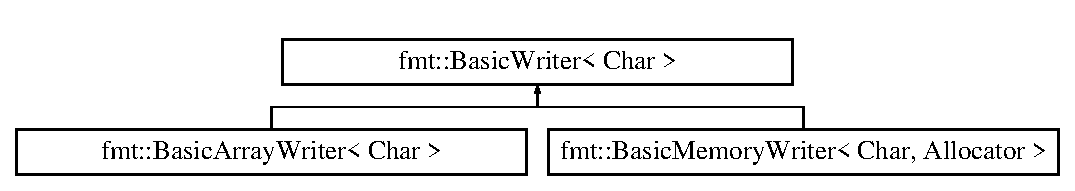
\includegraphics[height=2.000000cm]{classfmt_1_1BasicWriter}
\end{center}
\end{figure}
\subsection*{Public Member Functions}
\begin{DoxyCompactItemize}
\item 
virtual \hyperlink{classfmt_1_1BasicWriter_a25f6fc2e43d3bcfb3de9ac33afe6050d}{$\sim$\+Basic\+Writer} ()
\item 
std\+::size\+\_\+t \hyperlink{classfmt_1_1BasicWriter_a1b6721b4ba4d3fa18ac781a36616cc2a}{size} () const 
\item 
const Char $\ast$ \hyperlink{classfmt_1_1BasicWriter_a62d1c7b5be9c3580326320d5d178d096}{data} () const F\+M\+T\+\_\+\+N\+O\+E\+X\+C\+E\+PT
\item 
const Char $\ast$ \hyperlink{classfmt_1_1BasicWriter_a8b68001f5c1c0ea851ddaef27dcbc691}{c\+\_\+str} () const 
\item 
std\+::basic\+\_\+string$<$ Char $>$ \hyperlink{classfmt_1_1BasicWriter_a91f06ced6e063ee77a99740e0e79faf6}{str} () const 
\item 
void \hyperlink{classfmt_1_1BasicWriter_aaa83498c649d4a90ea3366bae62f4eac}{write} (\hyperlink{classfmt_1_1BasicCStringRef}{Basic\+C\+String\+Ref}$<$ Char $>$ format, \hyperlink{classfmt_1_1ArgList}{Arg\+List} args)
\item 
\hyperlink{classfmt_1_1BasicWriter}{Basic\+Writer} \& {\bfseries operator$<$$<$} (int value)\hypertarget{classfmt_1_1BasicWriter_a3d21148f336a76a71b39abb2fd6c0f88}{}\label{classfmt_1_1BasicWriter_a3d21148f336a76a71b39abb2fd6c0f88}

\item 
\hyperlink{classfmt_1_1BasicWriter}{Basic\+Writer} \& {\bfseries operator$<$$<$} (unsigned value)\hypertarget{classfmt_1_1BasicWriter_a7ec4d6fb4cf9173b14d4ee100fd4a428}{}\label{classfmt_1_1BasicWriter_a7ec4d6fb4cf9173b14d4ee100fd4a428}

\item 
\hyperlink{classfmt_1_1BasicWriter}{Basic\+Writer} \& {\bfseries operator$<$$<$} (long value)\hypertarget{classfmt_1_1BasicWriter_a1fd4183e01fd56ec99af40431b32561b}{}\label{classfmt_1_1BasicWriter_a1fd4183e01fd56ec99af40431b32561b}

\item 
\hyperlink{classfmt_1_1BasicWriter}{Basic\+Writer} \& {\bfseries operator$<$$<$} (unsigned long value)\hypertarget{classfmt_1_1BasicWriter_a4e0ef5415eb162ec991b69b930245094}{}\label{classfmt_1_1BasicWriter_a4e0ef5415eb162ec991b69b930245094}

\item 
\hyperlink{classfmt_1_1BasicWriter}{Basic\+Writer} \& {\bfseries operator$<$$<$} (Long\+Long value)\hypertarget{classfmt_1_1BasicWriter_a2c876284b0b3b7f36cc0354e3348912a}{}\label{classfmt_1_1BasicWriter_a2c876284b0b3b7f36cc0354e3348912a}

\item 
\hyperlink{classfmt_1_1BasicWriter}{Basic\+Writer} \& \hyperlink{classfmt_1_1BasicWriter_afb01c45f06b2c13027343b74ce973a40}{operator$<$$<$} (U\+Long\+Long value)
\item 
\hyperlink{classfmt_1_1BasicWriter}{Basic\+Writer} \& {\bfseries operator$<$$<$} (double value)\hypertarget{classfmt_1_1BasicWriter_afa435e67e3db3d214f0272b10c0a3878}{}\label{classfmt_1_1BasicWriter_afa435e67e3db3d214f0272b10c0a3878}

\item 
\hyperlink{classfmt_1_1BasicWriter}{Basic\+Writer} \& \hyperlink{classfmt_1_1BasicWriter_a90215ced4a6a9fcd5065f1ffd4105a4b}{operator$<$$<$} (long double value)
\item 
\hyperlink{classfmt_1_1BasicWriter}{Basic\+Writer} \& \hyperlink{classfmt_1_1BasicWriter_a4c7d6b3a40b4083f351de3f9ee0b3818}{operator$<$$<$} (char value)
\item 
\hyperlink{classfmt_1_1BasicWriter}{Basic\+Writer} \& {\bfseries operator$<$$<$} (typename \hyperlink{structfmt_1_1internal_1_1WCharHelper}{internal\+::\+W\+Char\+Helper}$<$ wchar\+\_\+t, Char $>$\+::Supported value)\hypertarget{classfmt_1_1BasicWriter_a83967e3236b090ba035d5fc04317f4ed}{}\label{classfmt_1_1BasicWriter_a83967e3236b090ba035d5fc04317f4ed}

\item 
\hyperlink{classfmt_1_1BasicWriter}{Basic\+Writer} \& \hyperlink{classfmt_1_1BasicWriter_a5f07d053b9f215b548ba3623e7a09212}{operator$<$$<$} (\hyperlink{classfmt_1_1BasicStringRef}{fmt\+::\+Basic\+String\+Ref}$<$ Char $>$ value)
\item 
\hyperlink{classfmt_1_1BasicWriter}{Basic\+Writer} \& {\bfseries operator$<$$<$} (typename \hyperlink{structfmt_1_1internal_1_1WCharHelper}{internal\+::\+W\+Char\+Helper}$<$ \hyperlink{classfmt_1_1BasicStringRef}{String\+Ref}, Char $>$\+::Supported value)\hypertarget{classfmt_1_1BasicWriter_ac0483272173279436f3d47f49894cafb}{}\label{classfmt_1_1BasicWriter_ac0483272173279436f3d47f49894cafb}

\item 
{\footnotesize template$<$typename T , typename Spec , typename Fill\+Char $>$ }\\\hyperlink{classfmt_1_1BasicWriter}{Basic\+Writer} \& {\bfseries operator$<$$<$} (\hyperlink{classfmt_1_1IntFormatSpec}{Int\+Format\+Spec}$<$ T, Spec, Fill\+Char $>$ spec)\hypertarget{classfmt_1_1BasicWriter_a45ded4f76427103f3c189855be8c5d46}{}\label{classfmt_1_1BasicWriter_a45ded4f76427103f3c189855be8c5d46}

\item 
{\footnotesize template$<$typename Str\+Char $>$ }\\\hyperlink{classfmt_1_1BasicWriter}{Basic\+Writer} \& {\bfseries operator$<$$<$} (const \hyperlink{classfmt_1_1StrFormatSpec}{Str\+Format\+Spec}$<$ Str\+Char $>$ \&spec)\hypertarget{classfmt_1_1BasicWriter_a79c23ed8ee17ee205ece04571f0dd79b}{}\label{classfmt_1_1BasicWriter_a79c23ed8ee17ee205ece04571f0dd79b}

\item 
void {\bfseries clear} () F\+M\+T\+\_\+\+N\+O\+E\+X\+C\+E\+PT\hypertarget{classfmt_1_1BasicWriter_aa5b6f4dd01854cbc3ebf06a7f2fce713}{}\label{classfmt_1_1BasicWriter_aa5b6f4dd01854cbc3ebf06a7f2fce713}

\item 
\hyperlink{classfmt_1_1Buffer}{Buffer}$<$ Char $>$ \& {\bfseries buffer} () F\+M\+T\+\_\+\+N\+O\+E\+X\+C\+E\+PT\hypertarget{classfmt_1_1BasicWriter_a9b2a71d2ec402005fca013111bb576cb}{}\label{classfmt_1_1BasicWriter_a9b2a71d2ec402005fca013111bb576cb}

\end{DoxyCompactItemize}
\subsection*{Protected Member Functions}
\begin{DoxyCompactItemize}
\item 
\hyperlink{classfmt_1_1BasicWriter_a586c21bbbd38149bcf48fc30376afc9c}{Basic\+Writer} (\hyperlink{classfmt_1_1Buffer}{Buffer}$<$ Char $>$ \&b)
\end{DoxyCompactItemize}
\subsection*{Friends}
\begin{DoxyCompactItemize}
\item 
{\footnotesize template$<$typename Impl , typename Char\+\_\+ $>$ }\\class {\bfseries internal\+::\+Arg\+Formatter\+Base}\hypertarget{classfmt_1_1BasicWriter_ac5db94b13180b25196a6e027c6efbfd7}{}\label{classfmt_1_1BasicWriter_ac5db94b13180b25196a6e027c6efbfd7}

\item 
class {\bfseries internal\+::\+Printf\+Arg\+Formatter$<$ Char $>$}\hypertarget{classfmt_1_1BasicWriter_a2a042c0745c912819e720759d8b498ae}{}\label{classfmt_1_1BasicWriter_a2a042c0745c912819e720759d8b498ae}

\end{DoxyCompactItemize}


\subsection{Detailed Description}
\subsubsection*{template$<$typename Char$>$\\*
class fmt\+::\+Basic\+Writer$<$ Char $>$}

This template provides operations for formatting and writing data into a character stream. The output is stored in a buffer provided by a subclass such as \+:class\+:{\ttfamily \hyperlink{classfmt_1_1BasicMemoryWriter}{fmt\+::\+Basic\+Memory\+Writer}}.

You can use one of the following typedefs for common character types\+:

+-\/-\/-\/-\/-\/-\/---+-\/-\/-\/-\/-\/-\/-\/-\/-\/-\/-\/-\/-\/-\/-\/-\/-\/-\/-\/---+ $\vert$ Type $\vert$ Definition $\vert$ +=========+======================+ $\vert$ Writer $\vert$ Basic\+Writer$<$char$>$ $\vert$ +-\/-\/-\/-\/-\/-\/---+-\/-\/-\/-\/-\/-\/-\/-\/-\/-\/-\/-\/-\/-\/-\/-\/-\/-\/-\/---+ $\vert$ W\+Writer $\vert$ Basic\+Writer$<$wchar\+\_\+t$>$ $\vert$ +-\/-\/-\/-\/-\/-\/---+-\/-\/-\/-\/-\/-\/-\/-\/-\/-\/-\/-\/-\/-\/-\/-\/-\/-\/-\/---+

\subsection{Constructor \& Destructor Documentation}
\index{fmt\+::\+Basic\+Writer@{fmt\+::\+Basic\+Writer}!Basic\+Writer@{Basic\+Writer}}
\index{Basic\+Writer@{Basic\+Writer}!fmt\+::\+Basic\+Writer@{fmt\+::\+Basic\+Writer}}
\subsubsection[{\texorpdfstring{Basic\+Writer(\+Buffer$<$ Char $>$ \&b)}{BasicWriter(Buffer< Char > &b)}}]{\setlength{\rightskip}{0pt plus 5cm}template$<$typename Char$>$ {\bf fmt\+::\+Basic\+Writer}$<$ Char $>$\+::{\bf Basic\+Writer} (
\begin{DoxyParamCaption}
\item[{{\bf Buffer}$<$ Char $>$ \&}]{b}
\end{DoxyParamCaption}
)\hspace{0.3cm}{\ttfamily [inline]}, {\ttfamily [explicit]}, {\ttfamily [protected]}}\hypertarget{classfmt_1_1BasicWriter_a586c21bbbd38149bcf48fc30376afc9c}{}\label{classfmt_1_1BasicWriter_a586c21bbbd38149bcf48fc30376afc9c}
Constructs a {\ttfamily \hyperlink{classfmt_1_1BasicWriter}{Basic\+Writer}} object. \index{fmt\+::\+Basic\+Writer@{fmt\+::\+Basic\+Writer}!````~Basic\+Writer@{$\sim$\+Basic\+Writer}}
\index{````~Basic\+Writer@{$\sim$\+Basic\+Writer}!fmt\+::\+Basic\+Writer@{fmt\+::\+Basic\+Writer}}
\subsubsection[{\texorpdfstring{$\sim$\+Basic\+Writer()}{~BasicWriter()}}]{\setlength{\rightskip}{0pt plus 5cm}template$<$typename Char$>$ virtual {\bf fmt\+::\+Basic\+Writer}$<$ Char $>$\+::$\sim${\bf Basic\+Writer} (
\begin{DoxyParamCaption}
{}
\end{DoxyParamCaption}
)\hspace{0.3cm}{\ttfamily [inline]}, {\ttfamily [virtual]}}\hypertarget{classfmt_1_1BasicWriter_a25f6fc2e43d3bcfb3de9ac33afe6050d}{}\label{classfmt_1_1BasicWriter_a25f6fc2e43d3bcfb3de9ac33afe6050d}
Destroys a {\ttfamily \hyperlink{classfmt_1_1BasicWriter}{Basic\+Writer}} object.  

\subsection{Member Function Documentation}
\index{fmt\+::\+Basic\+Writer@{fmt\+::\+Basic\+Writer}!c\+\_\+str@{c\+\_\+str}}
\index{c\+\_\+str@{c\+\_\+str}!fmt\+::\+Basic\+Writer@{fmt\+::\+Basic\+Writer}}
\subsubsection[{\texorpdfstring{c\+\_\+str() const }{c_str() const }}]{\setlength{\rightskip}{0pt plus 5cm}template$<$typename Char$>$ const Char$\ast$ {\bf fmt\+::\+Basic\+Writer}$<$ Char $>$\+::c\+\_\+str (
\begin{DoxyParamCaption}
{}
\end{DoxyParamCaption}
) const\hspace{0.3cm}{\ttfamily [inline]}}\hypertarget{classfmt_1_1BasicWriter_a8b68001f5c1c0ea851ddaef27dcbc691}{}\label{classfmt_1_1BasicWriter_a8b68001f5c1c0ea851ddaef27dcbc691}
Returns a pointer to the output buffer content with terminating null character appended. \index{fmt\+::\+Basic\+Writer@{fmt\+::\+Basic\+Writer}!data@{data}}
\index{data@{data}!fmt\+::\+Basic\+Writer@{fmt\+::\+Basic\+Writer}}
\subsubsection[{\texorpdfstring{data() const F\+M\+T\+\_\+\+N\+O\+E\+X\+C\+E\+PT}{data() const FMT_NOEXCEPT}}]{\setlength{\rightskip}{0pt plus 5cm}template$<$typename Char$>$ const Char$\ast$ {\bf fmt\+::\+Basic\+Writer}$<$ Char $>$\+::data (
\begin{DoxyParamCaption}
{}
\end{DoxyParamCaption}
) const\hspace{0.3cm}{\ttfamily [inline]}}\hypertarget{classfmt_1_1BasicWriter_a62d1c7b5be9c3580326320d5d178d096}{}\label{classfmt_1_1BasicWriter_a62d1c7b5be9c3580326320d5d178d096}
Returns a pointer to the output buffer content. No terminating null character is appended. \index{fmt\+::\+Basic\+Writer@{fmt\+::\+Basic\+Writer}!operator$<$$<$@{operator$<$$<$}}
\index{operator$<$$<$@{operator$<$$<$}!fmt\+::\+Basic\+Writer@{fmt\+::\+Basic\+Writer}}
\subsubsection[{\texorpdfstring{operator$<$$<$(\+U\+Long\+Long value)}{operator<<(ULongLong value)}}]{\setlength{\rightskip}{0pt plus 5cm}template$<$typename Char$>$ {\bf Basic\+Writer}\& {\bf fmt\+::\+Basic\+Writer}$<$ Char $>$\+::operator$<$$<$ (
\begin{DoxyParamCaption}
\item[{U\+Long\+Long}]{value}
\end{DoxyParamCaption}
)\hspace{0.3cm}{\ttfamily [inline]}}\hypertarget{classfmt_1_1BasicWriter_afb01c45f06b2c13027343b74ce973a40}{}\label{classfmt_1_1BasicWriter_afb01c45f06b2c13027343b74ce973a40}
Formats {\itshape value} and writes it to the stream.  \index{fmt\+::\+Basic\+Writer@{fmt\+::\+Basic\+Writer}!operator$<$$<$@{operator$<$$<$}}
\index{operator$<$$<$@{operator$<$$<$}!fmt\+::\+Basic\+Writer@{fmt\+::\+Basic\+Writer}}
\subsubsection[{\texorpdfstring{operator$<$$<$(long double value)}{operator<<(long double value)}}]{\setlength{\rightskip}{0pt plus 5cm}template$<$typename Char$>$ {\bf Basic\+Writer}\& {\bf fmt\+::\+Basic\+Writer}$<$ Char $>$\+::operator$<$$<$ (
\begin{DoxyParamCaption}
\item[{long double}]{value}
\end{DoxyParamCaption}
)\hspace{0.3cm}{\ttfamily [inline]}}\hypertarget{classfmt_1_1BasicWriter_a90215ced4a6a9fcd5065f1ffd4105a4b}{}\label{classfmt_1_1BasicWriter_a90215ced4a6a9fcd5065f1ffd4105a4b}
Formats {\itshape value} using the general format for floating-\/point numbers ({\ttfamily \textquotesingle{}g\textquotesingle{}}) and writes it to the stream.  \index{fmt\+::\+Basic\+Writer@{fmt\+::\+Basic\+Writer}!operator$<$$<$@{operator$<$$<$}}
\index{operator$<$$<$@{operator$<$$<$}!fmt\+::\+Basic\+Writer@{fmt\+::\+Basic\+Writer}}
\subsubsection[{\texorpdfstring{operator$<$$<$(char value)}{operator<<(char value)}}]{\setlength{\rightskip}{0pt plus 5cm}template$<$typename Char$>$ {\bf Basic\+Writer}\& {\bf fmt\+::\+Basic\+Writer}$<$ Char $>$\+::operator$<$$<$ (
\begin{DoxyParamCaption}
\item[{char}]{value}
\end{DoxyParamCaption}
)\hspace{0.3cm}{\ttfamily [inline]}}\hypertarget{classfmt_1_1BasicWriter_a4c7d6b3a40b4083f351de3f9ee0b3818}{}\label{classfmt_1_1BasicWriter_a4c7d6b3a40b4083f351de3f9ee0b3818}
Writes a character to the stream. \index{fmt\+::\+Basic\+Writer@{fmt\+::\+Basic\+Writer}!operator$<$$<$@{operator$<$$<$}}
\index{operator$<$$<$@{operator$<$$<$}!fmt\+::\+Basic\+Writer@{fmt\+::\+Basic\+Writer}}
\subsubsection[{\texorpdfstring{operator$<$$<$(fmt\+::\+Basic\+String\+Ref$<$ Char $>$ value)}{operator<<(fmt::BasicStringRef< Char > value)}}]{\setlength{\rightskip}{0pt plus 5cm}template$<$typename Char$>$ {\bf Basic\+Writer}\& {\bf fmt\+::\+Basic\+Writer}$<$ Char $>$\+::operator$<$$<$ (
\begin{DoxyParamCaption}
\item[{{\bf fmt\+::\+Basic\+String\+Ref}$<$ Char $>$}]{value}
\end{DoxyParamCaption}
)\hspace{0.3cm}{\ttfamily [inline]}}\hypertarget{classfmt_1_1BasicWriter_a5f07d053b9f215b548ba3623e7a09212}{}\label{classfmt_1_1BasicWriter_a5f07d053b9f215b548ba3623e7a09212}
Writes {\itshape value} to the stream.  \index{fmt\+::\+Basic\+Writer@{fmt\+::\+Basic\+Writer}!size@{size}}
\index{size@{size}!fmt\+::\+Basic\+Writer@{fmt\+::\+Basic\+Writer}}
\subsubsection[{\texorpdfstring{size() const }{size() const }}]{\setlength{\rightskip}{0pt plus 5cm}template$<$typename Char$>$ std\+::size\+\_\+t {\bf fmt\+::\+Basic\+Writer}$<$ Char $>$\+::size (
\begin{DoxyParamCaption}
{}
\end{DoxyParamCaption}
) const\hspace{0.3cm}{\ttfamily [inline]}}\hypertarget{classfmt_1_1BasicWriter_a1b6721b4ba4d3fa18ac781a36616cc2a}{}\label{classfmt_1_1BasicWriter_a1b6721b4ba4d3fa18ac781a36616cc2a}
Returns the total number of characters written. \index{fmt\+::\+Basic\+Writer@{fmt\+::\+Basic\+Writer}!str@{str}}
\index{str@{str}!fmt\+::\+Basic\+Writer@{fmt\+::\+Basic\+Writer}}
\subsubsection[{\texorpdfstring{str() const }{str() const }}]{\setlength{\rightskip}{0pt plus 5cm}template$<$typename Char$>$ std\+::basic\+\_\+string$<$Char$>$ {\bf fmt\+::\+Basic\+Writer}$<$ Char $>$\+::str (
\begin{DoxyParamCaption}
{}
\end{DoxyParamCaption}
) const\hspace{0.3cm}{\ttfamily [inline]}}\hypertarget{classfmt_1_1BasicWriter_a91f06ced6e063ee77a99740e0e79faf6}{}\label{classfmt_1_1BasicWriter_a91f06ced6e063ee77a99740e0e79faf6}
Returns the content of the output buffer as an {\ttfamily std\+::string}.  \index{fmt\+::\+Basic\+Writer@{fmt\+::\+Basic\+Writer}!write@{write}}
\index{write@{write}!fmt\+::\+Basic\+Writer@{fmt\+::\+Basic\+Writer}}
\subsubsection[{\texorpdfstring{write(\+Basic\+C\+String\+Ref$<$ Char $>$ format, Arg\+List args)}{write(BasicCStringRef< Char > format, ArgList args)}}]{\setlength{\rightskip}{0pt plus 5cm}template$<$typename Char$>$ void {\bf fmt\+::\+Basic\+Writer}$<$ Char $>$\+::write (
\begin{DoxyParamCaption}
\item[{{\bf Basic\+C\+String\+Ref}$<$ Char $>$}]{format, }
\item[{{\bf Arg\+List}}]{args}
\end{DoxyParamCaption}
)\hspace{0.3cm}{\ttfamily [inline]}}\hypertarget{classfmt_1_1BasicWriter_aaa83498c649d4a90ea3366bae62f4eac}{}\label{classfmt_1_1BasicWriter_aaa83498c649d4a90ea3366bae62f4eac}
Writes formatted data.

args$\ast$ is an argument list representing arbitrary arguments.

Example$\ast$$\ast$\+:\+:

Memory\+Writer out; out.\+write(\char`\"{}\+Current point\+:\textbackslash{}n\char`\"{}); out.\+write(\char`\"{}(\{\+:+f\}, \{\+:+f\})\char`\"{}, -\/3.\+14, 3.\+14);

This will write the following output to the {\ttfamily out} object\+:

.. code-\/block\+:\+: none

Current point\+: (-\/3.\+140000, +3.140000)

The output can be accessed using \+:func\+:{\ttfamily \hyperlink{classfmt_1_1BasicWriter_a62d1c7b5be9c3580326320d5d178d096}{data()}}, \+:func\+:{\ttfamily c\+\_\+str} or \+:func\+:{\ttfamily str} methods.

See also \+:ref\+:{\ttfamily syntax}.  

The documentation for this class was generated from the following file\+:\begin{DoxyCompactItemize}
\item 
cvdi-\/src/cvdi-\/cl/include/spdlog/fmt/bundled/format.\+h\end{DoxyCompactItemize}

\hypertarget{classcvdi__multi_1_1BatchParallel}{}\section{cvdi\+\_\+multi\+:\+:Batch\+Parallel Class Reference}
\label{classcvdi__multi_1_1BatchParallel}\index{cvdi\+\_\+multi\+::\+Batch\+Parallel@{cvdi\+\_\+multi\+::\+Batch\+Parallel}}


A class that processes files containing trips in parallel.  




{\ttfamily \#include $<$cvdi\+\_\+multi.\+hpp$>$}

Inheritance diagram for cvdi\+\_\+multi\+:\+:Batch\+Parallel\+:\begin{figure}[H]
\begin{center}
\leavevmode
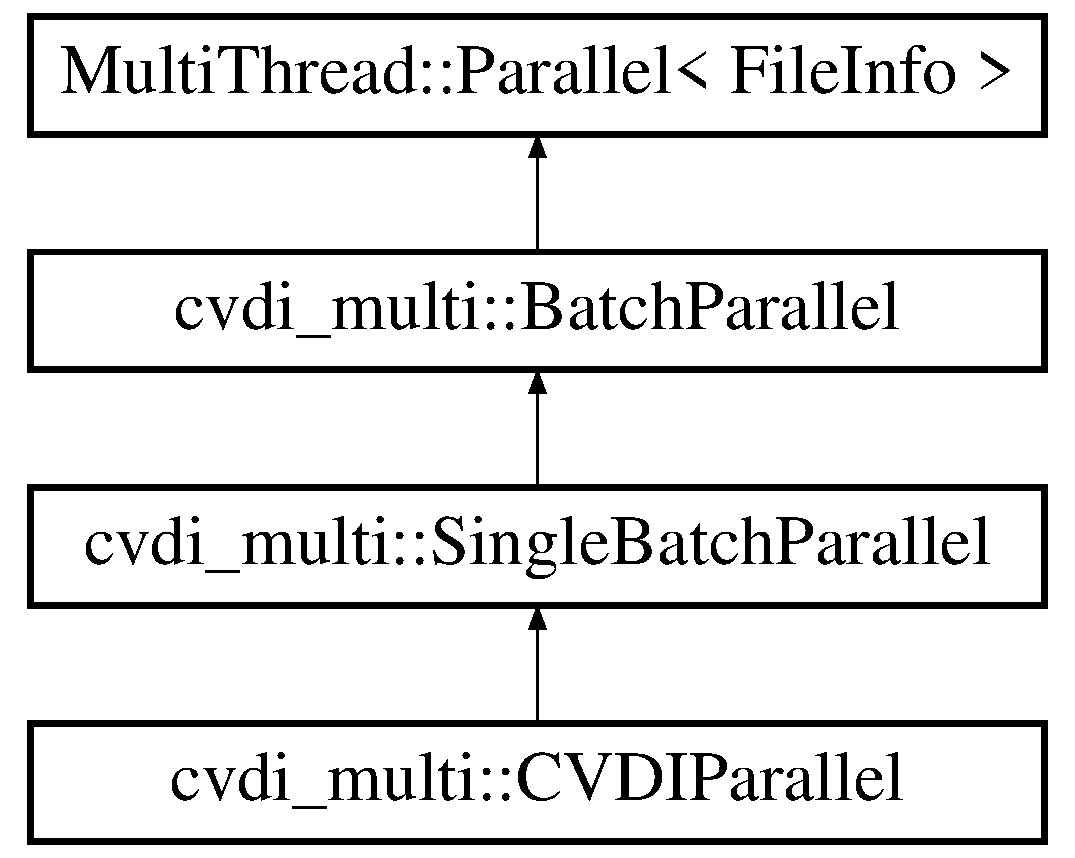
\includegraphics[height=4.000000cm]{classcvdi__multi_1_1BatchParallel}
\end{center}
\end{figure}
\subsection*{Public Member Functions}
\begin{DoxyCompactItemize}
\item 
\hyperlink{classcvdi__multi_1_1BatchParallel_ab759b92c4cd881df5ad39f8bfa940775}{Batch\+Parallel} (const std\+::string \&file\+\_\+path)
\begin{DoxyCompactList}\small\item\em Construct a batch processor that uses the provided file to find the trip files that needed to be processed. \end{DoxyCompactList}\item 
virtual void \hyperlink{classcvdi__multi_1_1BatchParallel_a23fd90da6768ad102e3ce5968ab11410}{Thread} (unsigned thread\+\_\+num, \hyperlink{classMultiThread_1_1SharedQueue}{Multi\+Thread\+::\+Shared\+Queue}$<$ File\+Info\+::\+Ptr $>$ $\ast$q)=0
\begin{DoxyCompactList}\small\item\em The main work thread. \end{DoxyCompactList}\item 
void \hyperlink{classcvdi__multi_1_1BatchParallel_a40f083a185b29a90733ada3fe789ada2}{Init} (unsigned n\+\_\+used\+\_\+threads)
\begin{DoxyCompactList}\small\item\em an initialization method; override to perform a concrete initialization action. \end{DoxyCompactList}\item 
void \hyperlink{classcvdi__multi_1_1BatchParallel_a5b9282057e92cd34460340a6f9625c8d}{Close} (void)\hypertarget{classcvdi__multi_1_1BatchParallel_a5b9282057e92cd34460340a6f9625c8d}{}\label{classcvdi__multi_1_1BatchParallel_a5b9282057e92cd34460340a6f9625c8d}

\begin{DoxyCompactList}\small\item\em Close the batch file. \end{DoxyCompactList}\item 
I\+F\+S\+Ptr {\bfseries Get\+File\+Ptr} (void) const \hypertarget{classcvdi__multi_1_1BatchParallel_a7d086bbc76e0a98821c4cadc1b6b3ed2}{}\label{classcvdi__multi_1_1BatchParallel_a7d086bbc76e0a98821c4cadc1b6b3ed2}

\item 
virtual File\+Info\+::\+Ptr {\bfseries Next\+Item} (void)=0\hypertarget{classcvdi__multi_1_1BatchParallel_add9bacacd5d698fdd077efcaa9c9c5f1}{}\label{classcvdi__multi_1_1BatchParallel_add9bacacd5d698fdd077efcaa9c9c5f1}

\end{DoxyCompactItemize}


\subsection{Detailed Description}
A class that processes files containing trips in parallel. 

\subsection{Constructor \& Destructor Documentation}
\index{cvdi\+\_\+multi\+::\+Batch\+Parallel@{cvdi\+\_\+multi\+::\+Batch\+Parallel}!Batch\+Parallel@{Batch\+Parallel}}
\index{Batch\+Parallel@{Batch\+Parallel}!cvdi\+\_\+multi\+::\+Batch\+Parallel@{cvdi\+\_\+multi\+::\+Batch\+Parallel}}
\subsubsection[{\texorpdfstring{Batch\+Parallel(const std\+::string \&file\+\_\+path)}{BatchParallel(const std::string &file_path)}}]{\setlength{\rightskip}{0pt plus 5cm}cvdi\+\_\+multi\+::\+Batch\+Parallel\+::\+Batch\+Parallel (
\begin{DoxyParamCaption}
\item[{const std\+::string \&}]{file\+\_\+path}
\end{DoxyParamCaption}
)}\hypertarget{classcvdi__multi_1_1BatchParallel_ab759b92c4cd881df5ad39f8bfa940775}{}\label{classcvdi__multi_1_1BatchParallel_ab759b92c4cd881df5ad39f8bfa940775}


Construct a batch processor that uses the provided file to find the trip files that needed to be processed. 


\begin{DoxyParams}{Parameters}
{\em file\+\_\+path} & a file having a trip file on each line. \\
\hline
\end{DoxyParams}


\subsection{Member Function Documentation}
\index{cvdi\+\_\+multi\+::\+Batch\+Parallel@{cvdi\+\_\+multi\+::\+Batch\+Parallel}!Init@{Init}}
\index{Init@{Init}!cvdi\+\_\+multi\+::\+Batch\+Parallel@{cvdi\+\_\+multi\+::\+Batch\+Parallel}}
\subsubsection[{\texorpdfstring{Init(unsigned n\+\_\+used\+\_\+threads)}{Init(unsigned n_used_threads)}}]{\setlength{\rightskip}{0pt plus 5cm}void cvdi\+\_\+multi\+::\+Batch\+Parallel\+::\+Init (
\begin{DoxyParamCaption}
\item[{unsigned}]{n\+\_\+used\+\_\+threads}
\end{DoxyParamCaption}
)\hspace{0.3cm}{\ttfamily [virtual]}}\hypertarget{classcvdi__multi_1_1BatchParallel_a40f083a185b29a90733ada3fe789ada2}{}\label{classcvdi__multi_1_1BatchParallel_a40f083a185b29a90733ada3fe789ada2}


an initialization method; override to perform a concrete initialization action. 


\begin{DoxyParams}{Parameters}
{\em n\+\_\+used\+\_\+threads} & the number of threads that will be managed by this instance. \\
\hline
\end{DoxyParams}


Implements \hyperlink{classMultiThread_1_1Parallel}{Multi\+Thread\+::\+Parallel$<$ File\+Info $>$}.



Reimplemented in \hyperlink{classcvdi__multi_1_1CVDIParallel_a5d162d98140883424d43acd01c562507}{cvdi\+\_\+multi\+::\+C\+V\+D\+I\+Parallel}.

\index{cvdi\+\_\+multi\+::\+Batch\+Parallel@{cvdi\+\_\+multi\+::\+Batch\+Parallel}!Thread@{Thread}}
\index{Thread@{Thread}!cvdi\+\_\+multi\+::\+Batch\+Parallel@{cvdi\+\_\+multi\+::\+Batch\+Parallel}}
\subsubsection[{\texorpdfstring{Thread(unsigned thread\+\_\+num, Multi\+Thread\+::\+Shared\+Queue$<$ File\+Info\+::\+Ptr $>$ $\ast$q)=0}{Thread(unsigned thread_num, MultiThread::SharedQueue< FileInfo::Ptr > *q)=0}}]{\setlength{\rightskip}{0pt plus 5cm}virtual void cvdi\+\_\+multi\+::\+Batch\+Parallel\+::\+Thread (
\begin{DoxyParamCaption}
\item[{unsigned}]{thread\+\_\+num, }
\item[{{\bf Multi\+Thread\+::\+Shared\+Queue}$<$ File\+Info\+::\+Ptr $>$ $\ast$}]{q}
\end{DoxyParamCaption}
)\hspace{0.3cm}{\ttfamily [pure virtual]}}\hypertarget{classcvdi__multi_1_1BatchParallel_a23fd90da6768ad102e3ce5968ab11410}{}\label{classcvdi__multi_1_1BatchParallel_a23fd90da6768ad102e3ce5968ab11410}


The main work thread. 


\begin{DoxyParams}{Parameters}
{\em thread\+\_\+num} & a easy to read unique identifier for this thread. \\
\hline
{\em the} & work queue containing the trip files that this thread should process. \\
\hline
\end{DoxyParams}


Implemented in \hyperlink{classcvdi__multi_1_1CVDIParallel_a7c256d91bb868873a1c6ce854c923c17}{cvdi\+\_\+multi\+::\+C\+V\+D\+I\+Parallel}, and \hyperlink{classcvdi__multi_1_1SingleBatchParallel_a6514a89e14f2724ab671ffd65d7c43c7}{cvdi\+\_\+multi\+::\+Single\+Batch\+Parallel}.



The documentation for this class was generated from the following files\+:\begin{DoxyCompactItemize}
\item 
cvdi-\/src/cvdi-\/cl/include/cvdi\+\_\+multi.\+hpp\item 
cvdi-\/src/cvdi-\/cl/src/cvdi\+\_\+multi.\+cpp\end{DoxyCompactItemize}

\hypertarget{classfmt_1_1Buffer}{}\section{fmt\+:\+:Buffer$<$ T $>$ Class Template Reference}
\label{classfmt_1_1Buffer}\index{fmt\+::\+Buffer$<$ T $>$@{fmt\+::\+Buffer$<$ T $>$}}


{\ttfamily \#include $<$format.\+h$>$}

Inheritance diagram for fmt\+:\+:Buffer$<$ T $>$\+:\begin{figure}[H]
\begin{center}
\leavevmode
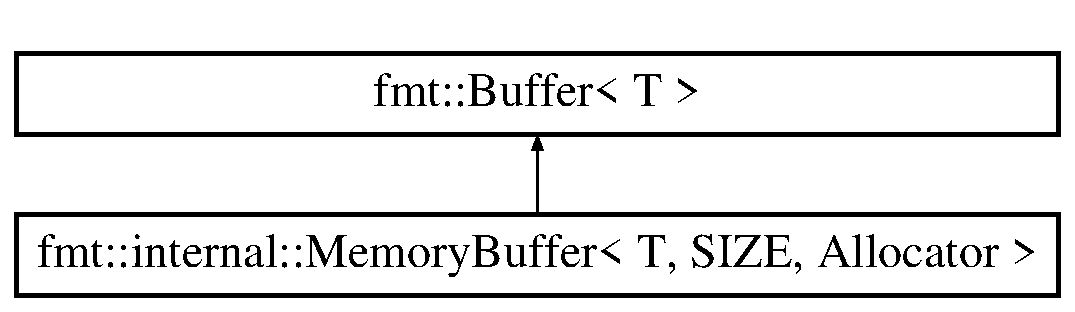
\includegraphics[height=2.000000cm]{classfmt_1_1Buffer}
\end{center}
\end{figure}
\subsection*{Public Member Functions}
\begin{DoxyCompactItemize}
\item 
std\+::size\+\_\+t \hyperlink{classfmt_1_1Buffer_a14fa72f0ddf584c14ffffb1446f598aa}{size} () const 
\item 
std\+::size\+\_\+t \hyperlink{classfmt_1_1Buffer_aaf54fe786de91157629f96380e0cb215}{capacity} () const 
\item 
void \hyperlink{classfmt_1_1Buffer_a20f893164dc20e8ea8c77810d4ea8d59}{resize} (std\+::size\+\_\+t new\+\_\+size)
\item 
void \hyperlink{classfmt_1_1Buffer_a7f46a3ce8d86abe35904f6654bd4ea1e}{reserve} (std\+::size\+\_\+t \hyperlink{classfmt_1_1Buffer_aaf54fe786de91157629f96380e0cb215}{capacity})
\item 
void {\bfseries clear} () F\+M\+T\+\_\+\+N\+O\+E\+X\+C\+E\+PT\hypertarget{classfmt_1_1Buffer_a4591d21c7970ba5205680cb5224ef2b2}{}\label{classfmt_1_1Buffer_a4591d21c7970ba5205680cb5224ef2b2}

\item 
void {\bfseries push\+\_\+back} (const T \&value)\hypertarget{classfmt_1_1Buffer_a4056b71637286b41b3275e3dac57462d}{}\label{classfmt_1_1Buffer_a4056b71637286b41b3275e3dac57462d}

\item 
{\footnotesize template$<$typename U $>$ }\\void \hyperlink{classfmt_1_1Buffer_a7ca155741c43ec7c7edcea8dd28a2123}{append} (const U $\ast$begin, const U $\ast$end)
\item 
T \& {\bfseries operator\mbox{[}$\,$\mbox{]}} (std\+::size\+\_\+t index)\hypertarget{classfmt_1_1Buffer_ad1f9ad75ba08826671a78df23161685a}{}\label{classfmt_1_1Buffer_ad1f9ad75ba08826671a78df23161685a}

\item 
const T \& {\bfseries operator\mbox{[}$\,$\mbox{]}} (std\+::size\+\_\+t index) const \hypertarget{classfmt_1_1Buffer_a15dd7f9027d6c9fb0fe4b6255c9a7929}{}\label{classfmt_1_1Buffer_a15dd7f9027d6c9fb0fe4b6255c9a7929}

\end{DoxyCompactItemize}
\subsection*{Protected Member Functions}
\begin{DoxyCompactItemize}
\item 
{\bfseries Buffer} (T $\ast$ptr=0, std\+::size\+\_\+t \hyperlink{classfmt_1_1Buffer_aaf54fe786de91157629f96380e0cb215}{capacity}=0)\hypertarget{classfmt_1_1Buffer_a1830c1ba88170ed60f40f662d7f1886a}{}\label{classfmt_1_1Buffer_a1830c1ba88170ed60f40f662d7f1886a}

\item 
virtual void \hyperlink{classfmt_1_1Buffer_abdc7aaf5813aa07008b3d715969a7e19}{grow} (std\+::size\+\_\+t \hyperlink{classfmt_1_1Buffer_a14fa72f0ddf584c14ffffb1446f598aa}{size})=0
\end{DoxyCompactItemize}
\subsection*{Protected Attributes}
\begin{DoxyCompactItemize}
\item 
T $\ast$ {\bfseries ptr\+\_\+}\hypertarget{classfmt_1_1Buffer_a17b11ccf916407fdb464b53b3e556849}{}\label{classfmt_1_1Buffer_a17b11ccf916407fdb464b53b3e556849}

\item 
std\+::size\+\_\+t {\bfseries size\+\_\+}\hypertarget{classfmt_1_1Buffer_a3959d66180b075a0ae324ea98466e20f}{}\label{classfmt_1_1Buffer_a3959d66180b075a0ae324ea98466e20f}

\item 
std\+::size\+\_\+t {\bfseries capacity\+\_\+}\hypertarget{classfmt_1_1Buffer_ab9c3e293679699058a2d33c4a07ad657}{}\label{classfmt_1_1Buffer_ab9c3e293679699058a2d33c4a07ad657}

\end{DoxyCompactItemize}


\subsection{Detailed Description}
\subsubsection*{template$<$typename T$>$\\*
class fmt\+::\+Buffer$<$ T $>$}

A buffer supporting a subset of {\ttfamily std\+::vector}\textquotesingle{}s operations.  

\subsection{Member Function Documentation}
\index{fmt\+::\+Buffer@{fmt\+::\+Buffer}!append@{append}}
\index{append@{append}!fmt\+::\+Buffer@{fmt\+::\+Buffer}}
\subsubsection[{\texorpdfstring{append(const U $\ast$begin, const U $\ast$end)}{append(const U *begin, const U *end)}}]{\setlength{\rightskip}{0pt plus 5cm}template$<$typename T $>$ template$<$typename U $>$ void {\bf fmt\+::\+Buffer}$<$ T $>$\+::append (
\begin{DoxyParamCaption}
\item[{const U $\ast$}]{begin, }
\item[{const U $\ast$}]{end}
\end{DoxyParamCaption}
)}\hypertarget{classfmt_1_1Buffer_a7ca155741c43ec7c7edcea8dd28a2123}{}\label{classfmt_1_1Buffer_a7ca155741c43ec7c7edcea8dd28a2123}
Appends data to the end of the buffer. \index{fmt\+::\+Buffer@{fmt\+::\+Buffer}!capacity@{capacity}}
\index{capacity@{capacity}!fmt\+::\+Buffer@{fmt\+::\+Buffer}}
\subsubsection[{\texorpdfstring{capacity() const }{capacity() const }}]{\setlength{\rightskip}{0pt plus 5cm}template$<$typename T$>$ std\+::size\+\_\+t {\bf fmt\+::\+Buffer}$<$ T $>$\+::capacity (
\begin{DoxyParamCaption}
{}
\end{DoxyParamCaption}
) const\hspace{0.3cm}{\ttfamily [inline]}}\hypertarget{classfmt_1_1Buffer_aaf54fe786de91157629f96380e0cb215}{}\label{classfmt_1_1Buffer_aaf54fe786de91157629f96380e0cb215}
Returns the capacity of this buffer. \index{fmt\+::\+Buffer@{fmt\+::\+Buffer}!grow@{grow}}
\index{grow@{grow}!fmt\+::\+Buffer@{fmt\+::\+Buffer}}
\subsubsection[{\texorpdfstring{grow(std\+::size\+\_\+t size)=0}{grow(std::size_t size)=0}}]{\setlength{\rightskip}{0pt plus 5cm}template$<$typename T$>$ virtual void {\bf fmt\+::\+Buffer}$<$ T $>$\+::grow (
\begin{DoxyParamCaption}
\item[{std\+::size\+\_\+t}]{size}
\end{DoxyParamCaption}
)\hspace{0.3cm}{\ttfamily [protected]}, {\ttfamily [pure virtual]}}\hypertarget{classfmt_1_1Buffer_abdc7aaf5813aa07008b3d715969a7e19}{}\label{classfmt_1_1Buffer_abdc7aaf5813aa07008b3d715969a7e19}
Increases the buffer capacity to hold at least {\itshape size} elements updating {\ttfamily ptr\+\_\+} and {\ttfamily capacity\+\_\+}.  

Implemented in \hyperlink{classfmt_1_1internal_1_1FixedBuffer_a90dc1dce4e8eac799d57ca519cfeb82d}{fmt\+::internal\+::\+Fixed\+Buffer$<$ Char $>$}, \hyperlink{classfmt_1_1internal_1_1MemoryBuffer_a6ecee679d5caf3345f8ffae92b7ca702}{fmt\+::internal\+::\+Memory\+Buffer$<$ T, S\+I\+Z\+E, Allocator $>$}, and \hyperlink{classfmt_1_1internal_1_1MemoryBuffer_a6ecee679d5caf3345f8ffae92b7ca702}{fmt\+::internal\+::\+Memory\+Buffer$<$ Char, internal\+::\+I\+N\+L\+I\+N\+E\+\_\+\+B\+U\+F\+F\+E\+R\+\_\+\+S\+I\+Z\+E, Allocator $>$}.

\index{fmt\+::\+Buffer@{fmt\+::\+Buffer}!reserve@{reserve}}
\index{reserve@{reserve}!fmt\+::\+Buffer@{fmt\+::\+Buffer}}
\subsubsection[{\texorpdfstring{reserve(std\+::size\+\_\+t capacity)}{reserve(std::size_t capacity)}}]{\setlength{\rightskip}{0pt plus 5cm}template$<$typename T$>$ void {\bf fmt\+::\+Buffer}$<$ T $>$\+::reserve (
\begin{DoxyParamCaption}
\item[{std\+::size\+\_\+t}]{capacity}
\end{DoxyParamCaption}
)\hspace{0.3cm}{\ttfamily [inline]}}\hypertarget{classfmt_1_1Buffer_a7f46a3ce8d86abe35904f6654bd4ea1e}{}\label{classfmt_1_1Buffer_a7f46a3ce8d86abe35904f6654bd4ea1e}
Reserves space to store at least {\itshape capacity} elements.  \index{fmt\+::\+Buffer@{fmt\+::\+Buffer}!resize@{resize}}
\index{resize@{resize}!fmt\+::\+Buffer@{fmt\+::\+Buffer}}
\subsubsection[{\texorpdfstring{resize(std\+::size\+\_\+t new\+\_\+size)}{resize(std::size_t new_size)}}]{\setlength{\rightskip}{0pt plus 5cm}template$<$typename T$>$ void {\bf fmt\+::\+Buffer}$<$ T $>$\+::resize (
\begin{DoxyParamCaption}
\item[{std\+::size\+\_\+t}]{new\+\_\+size}
\end{DoxyParamCaption}
)\hspace{0.3cm}{\ttfamily [inline]}}\hypertarget{classfmt_1_1Buffer_a20f893164dc20e8ea8c77810d4ea8d59}{}\label{classfmt_1_1Buffer_a20f893164dc20e8ea8c77810d4ea8d59}
Resizes the buffer. If T is a P\+OD type new elements may not be initialized. \index{fmt\+::\+Buffer@{fmt\+::\+Buffer}!size@{size}}
\index{size@{size}!fmt\+::\+Buffer@{fmt\+::\+Buffer}}
\subsubsection[{\texorpdfstring{size() const }{size() const }}]{\setlength{\rightskip}{0pt plus 5cm}template$<$typename T$>$ std\+::size\+\_\+t {\bf fmt\+::\+Buffer}$<$ T $>$\+::size (
\begin{DoxyParamCaption}
{}
\end{DoxyParamCaption}
) const\hspace{0.3cm}{\ttfamily [inline]}}\hypertarget{classfmt_1_1Buffer_a14fa72f0ddf584c14ffffb1446f598aa}{}\label{classfmt_1_1Buffer_a14fa72f0ddf584c14ffffb1446f598aa}
Returns the size of this buffer. 

The documentation for this class was generated from the following file\+:\begin{DoxyCompactItemize}
\item 
cvdi-\/src/cvdi-\/cl/include/spdlog/fmt/bundled/format.\+h\end{DoxyCompactItemize}

\hypertarget{classfmt_1_1BufferedFile}{}\section{fmt\+:\+:Buffered\+File Class Reference}
\label{classfmt_1_1BufferedFile}\index{fmt\+::\+Buffered\+File@{fmt\+::\+Buffered\+File}}
\subsection*{Public Member Functions}
\begin{DoxyCompactItemize}
\item 
{\bfseries Buffered\+File} (Proxy p) F\+M\+T\+\_\+\+N\+O\+E\+X\+C\+E\+PT\hypertarget{classfmt_1_1BufferedFile_a893b570968946b0f0f54c32a4c9742b6}{}\label{classfmt_1_1BufferedFile_a893b570968946b0f0f54c32a4c9742b6}

\item 
{\bfseries Buffered\+File} (\hyperlink{classfmt_1_1BufferedFile}{Buffered\+File} \&f) F\+M\+T\+\_\+\+N\+O\+E\+X\+C\+E\+PT\hypertarget{classfmt_1_1BufferedFile_a5bc528da7a6888f44a2f753cef3a7a09}{}\label{classfmt_1_1BufferedFile_a5bc528da7a6888f44a2f753cef3a7a09}

\item 
\hyperlink{classfmt_1_1BufferedFile}{Buffered\+File} \& {\bfseries operator=} (Proxy p)\hypertarget{classfmt_1_1BufferedFile_a03830cce82e5afbf2ddc39f3132db199}{}\label{classfmt_1_1BufferedFile_a03830cce82e5afbf2ddc39f3132db199}

\item 
\hyperlink{classfmt_1_1BufferedFile}{Buffered\+File} \& {\bfseries operator=} (\hyperlink{classfmt_1_1BufferedFile}{Buffered\+File} \&other)\hypertarget{classfmt_1_1BufferedFile_ad517d6edd8d0cff10e12abc7210431fc}{}\label{classfmt_1_1BufferedFile_ad517d6edd8d0cff10e12abc7210431fc}

\item 
{\bfseries operator Proxy} () F\+M\+T\+\_\+\+N\+O\+E\+X\+C\+E\+PT\hypertarget{classfmt_1_1BufferedFile_a54ffb69364af7d25bc8b19eb4e901ac5}{}\label{classfmt_1_1BufferedFile_a54ffb69364af7d25bc8b19eb4e901ac5}

\item 
{\bfseries Buffered\+File} (\hyperlink{classfmt_1_1BasicCStringRef}{C\+String\+Ref} filename, \hyperlink{classfmt_1_1BasicCStringRef}{C\+String\+Ref} mode)\hypertarget{classfmt_1_1BufferedFile_a5a2e3a0aabc752eb52993ea2488c95a8}{}\label{classfmt_1_1BufferedFile_a5a2e3a0aabc752eb52993ea2488c95a8}

\item 
void {\bfseries close} ()\hypertarget{classfmt_1_1BufferedFile_ad9b8340d0a6b638ef0ab83c7bed3d554}{}\label{classfmt_1_1BufferedFile_ad9b8340d0a6b638ef0ab83c7bed3d554}

\item 
F\+I\+LE $\ast$ {\bfseries get} () const F\+M\+T\+\_\+\+N\+O\+E\+X\+C\+E\+PT\hypertarget{classfmt_1_1BufferedFile_a2702f924d04db7f93b7512dd12ba79df}{}\label{classfmt_1_1BufferedFile_a2702f924d04db7f93b7512dd12ba79df}

\item 
int() {\bfseries fileno} () const \hypertarget{classfmt_1_1BufferedFile_a12330a2aa3b372295020e3b2d973f8ae}{}\label{classfmt_1_1BufferedFile_a12330a2aa3b372295020e3b2d973f8ae}

\item 
void {\bfseries print} (\hyperlink{classfmt_1_1BasicCStringRef}{C\+String\+Ref} format\+\_\+str, const \hyperlink{classfmt_1_1ArgList}{Arg\+List} \&args)\hypertarget{classfmt_1_1BufferedFile_aa07aa36b56d75a0e8db27d1790a8266c}{}\label{classfmt_1_1BufferedFile_aa07aa36b56d75a0e8db27d1790a8266c}

\end{DoxyCompactItemize}
\subsection*{Friends}
\begin{DoxyCompactItemize}
\item 
class {\bfseries File}\hypertarget{classfmt_1_1BufferedFile_a68d15876ad188b7628261b12d0eac8aa}{}\label{classfmt_1_1BufferedFile_a68d15876ad188b7628261b12d0eac8aa}

\end{DoxyCompactItemize}


The documentation for this class was generated from the following files\+:\begin{DoxyCompactItemize}
\item 
cvdi-\/src/cvdi-\/cl/include/spdlog/fmt/bundled/posix.\+h\item 
cvdi-\/src/cvdi-\/cl/include/spdlog/fmt/bundled/posix.\+cc\end{DoxyCompactItemize}

\hypertarget{classfmt_1_1internal_1_1CharTraits}{}\section{fmt\+:\+:internal\+:\+:Char\+Traits$<$ Char $>$ Class Template Reference}
\label{classfmt_1_1internal_1_1CharTraits}\index{fmt\+::internal\+::\+Char\+Traits$<$ Char $>$@{fmt\+::internal\+::\+Char\+Traits$<$ Char $>$}}


The documentation for this class was generated from the following file\+:\begin{DoxyCompactItemize}
\item 
cvdi-\/src/cvdi-\/cl/include/spdlog/fmt/bundled/format.\+h\end{DoxyCompactItemize}

\hypertarget{classfmt_1_1internal_1_1CharTraits_3_01char_01_4}{}\section{fmt\+:\+:internal\+:\+:Char\+Traits$<$ char $>$ Class Template Reference}
\label{classfmt_1_1internal_1_1CharTraits_3_01char_01_4}\index{fmt\+::internal\+::\+Char\+Traits$<$ char $>$@{fmt\+::internal\+::\+Char\+Traits$<$ char $>$}}
Inheritance diagram for fmt\+:\+:internal\+:\+:Char\+Traits$<$ char $>$\+:\begin{figure}[H]
\begin{center}
\leavevmode
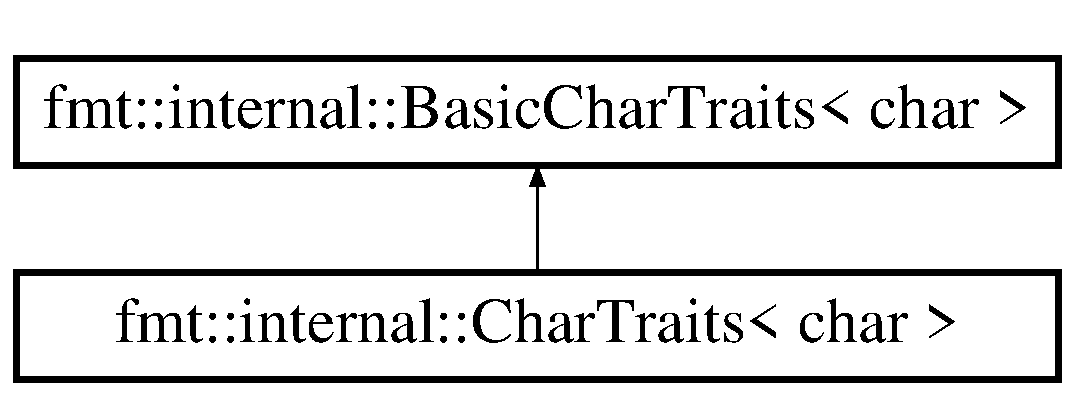
\includegraphics[height=2.000000cm]{classfmt_1_1internal_1_1CharTraits_3_01char_01_4}
\end{center}
\end{figure}
\subsection*{Public Member Functions}
\begin{DoxyCompactItemize}
\item 
{\footnotesize template$<$typename T $>$ }\\int {\bfseries format\+\_\+float} (char $\ast$buffer, std\+::size\+\_\+t size, const char $\ast$format, unsigned width, int precision, T value)\hypertarget{classfmt_1_1internal_1_1CharTraits_3_01char_01_4_a378a229c5a4846ffa8f4eb119534a002}{}\label{classfmt_1_1internal_1_1CharTraits_3_01char_01_4_a378a229c5a4846ffa8f4eb119534a002}

\end{DoxyCompactItemize}
\subsection*{Static Public Member Functions}
\begin{DoxyCompactItemize}
\item 
static char {\bfseries convert} (char value)\hypertarget{classfmt_1_1internal_1_1CharTraits_3_01char_01_4_a4503977c29c6347f94b829728c42997c}{}\label{classfmt_1_1internal_1_1CharTraits_3_01char_01_4_a4503977c29c6347f94b829728c42997c}

\item 
{\footnotesize template$<$typename T $>$ }\\static F\+M\+T\+\_\+\+A\+PI int {\bfseries format\+\_\+float} (char $\ast$buffer, std\+::size\+\_\+t size, const char $\ast$format, unsigned width, int precision, T value)\hypertarget{classfmt_1_1internal_1_1CharTraits_3_01char_01_4_a0ae1f571ad4676bbc4ff7aafb5312176}{}\label{classfmt_1_1internal_1_1CharTraits_3_01char_01_4_a0ae1f571ad4676bbc4ff7aafb5312176}

\end{DoxyCompactItemize}
\subsection*{Additional Inherited Members}


The documentation for this class was generated from the following files\+:\begin{DoxyCompactItemize}
\item 
cvdi-\/src/cvdi-\/cl/include/spdlog/fmt/bundled/format.\+h\item 
cvdi-\/src/cvdi-\/cl/include/spdlog/fmt/bundled/format.\+cc\end{DoxyCompactItemize}

\hypertarget{classfmt_1_1internal_1_1CharTraits_3_01wchar__t_01_4}{}\section{fmt\+:\+:internal\+:\+:Char\+Traits$<$ wchar\+\_\+t $>$ Class Template Reference}
\label{classfmt_1_1internal_1_1CharTraits_3_01wchar__t_01_4}\index{fmt\+::internal\+::\+Char\+Traits$<$ wchar\+\_\+t $>$@{fmt\+::internal\+::\+Char\+Traits$<$ wchar\+\_\+t $>$}}
Inheritance diagram for fmt\+:\+:internal\+:\+:Char\+Traits$<$ wchar\+\_\+t $>$\+:\begin{figure}[H]
\begin{center}
\leavevmode
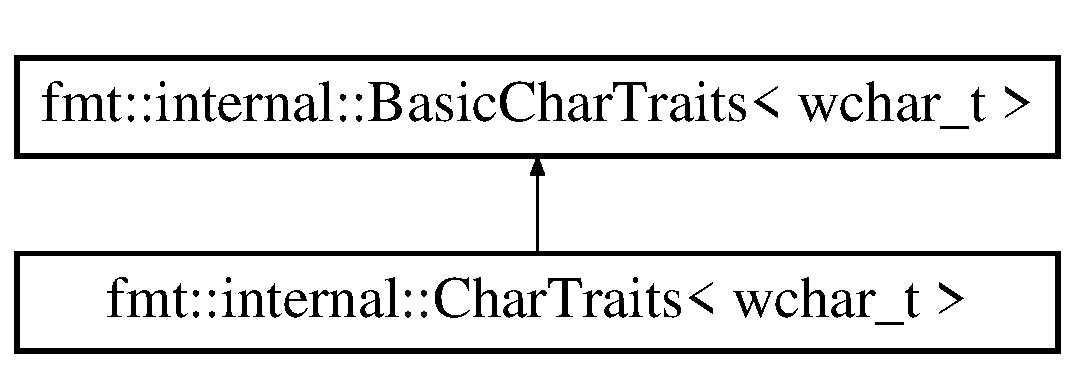
\includegraphics[height=2.000000cm]{classfmt_1_1internal_1_1CharTraits_3_01wchar__t_01_4}
\end{center}
\end{figure}
\subsection*{Public Member Functions}
\begin{DoxyCompactItemize}
\item 
{\footnotesize template$<$typename T $>$ }\\int {\bfseries format\+\_\+float} (wchar\+\_\+t $\ast$buffer, std\+::size\+\_\+t size, const wchar\+\_\+t $\ast$format, unsigned width, int precision, T value)\hypertarget{classfmt_1_1internal_1_1CharTraits_3_01wchar__t_01_4_aed134df338cc820d428797528dab4666}{}\label{classfmt_1_1internal_1_1CharTraits_3_01wchar__t_01_4_aed134df338cc820d428797528dab4666}

\end{DoxyCompactItemize}
\subsection*{Static Public Member Functions}
\begin{DoxyCompactItemize}
\item 
static wchar\+\_\+t {\bfseries convert} (char value)\hypertarget{classfmt_1_1internal_1_1CharTraits_3_01wchar__t_01_4_aca94c09c993fa75d2a518d519f6fc177}{}\label{classfmt_1_1internal_1_1CharTraits_3_01wchar__t_01_4_aca94c09c993fa75d2a518d519f6fc177}

\item 
static wchar\+\_\+t {\bfseries convert} (wchar\+\_\+t value)\hypertarget{classfmt_1_1internal_1_1CharTraits_3_01wchar__t_01_4_adbfb38618bd648c3fb4220071d433093}{}\label{classfmt_1_1internal_1_1CharTraits_3_01wchar__t_01_4_adbfb38618bd648c3fb4220071d433093}

\item 
{\footnotesize template$<$typename T $>$ }\\static F\+M\+T\+\_\+\+A\+PI int {\bfseries format\+\_\+float} (wchar\+\_\+t $\ast$buffer, std\+::size\+\_\+t size, const wchar\+\_\+t $\ast$format, unsigned width, int precision, T value)\hypertarget{classfmt_1_1internal_1_1CharTraits_3_01wchar__t_01_4_a72c61dfaffb6965a9e78b28e3f7a3538}{}\label{classfmt_1_1internal_1_1CharTraits_3_01wchar__t_01_4_a72c61dfaffb6965a9e78b28e3f7a3538}

\end{DoxyCompactItemize}
\subsection*{Additional Inherited Members}


The documentation for this class was generated from the following files\+:\begin{DoxyCompactItemize}
\item 
cvdi-\/src/cvdi-\/cl/include/spdlog/fmt/bundled/format.\+h\item 
cvdi-\/src/cvdi-\/cl/include/spdlog/fmt/bundled/format.\+cc\end{DoxyCompactItemize}

\hypertarget{structfmt_1_1internal_1_1Conditional}{}\section{fmt\+:\+:internal\+:\+:Conditional$<$ B, T, F $>$ Struct Template Reference}
\label{structfmt_1_1internal_1_1Conditional}\index{fmt\+::internal\+::\+Conditional$<$ B, T, F $>$@{fmt\+::internal\+::\+Conditional$<$ B, T, F $>$}}
\subsection*{Public Types}
\begin{DoxyCompactItemize}
\item 
typedef T {\bfseries type}\hypertarget{structfmt_1_1internal_1_1Conditional_a2670cd09823078e9ac3d59e8ad5e9e5e}{}\label{structfmt_1_1internal_1_1Conditional_a2670cd09823078e9ac3d59e8ad5e9e5e}

\end{DoxyCompactItemize}


The documentation for this struct was generated from the following file\+:\begin{DoxyCompactItemize}
\item 
cvdi-\/src/cvdi-\/cl/include/spdlog/fmt/bundled/format.\+h\end{DoxyCompactItemize}

\hypertarget{structfmt_1_1internal_1_1Conditional_3_01false_00_01T_00_01F_01_4}{}\section{fmt\+:\+:internal\+:\+:Conditional$<$ false, T, F $>$ Struct Template Reference}
\label{structfmt_1_1internal_1_1Conditional_3_01false_00_01T_00_01F_01_4}\index{fmt\+::internal\+::\+Conditional$<$ false, T, F $>$@{fmt\+::internal\+::\+Conditional$<$ false, T, F $>$}}
\subsection*{Public Types}
\begin{DoxyCompactItemize}
\item 
typedef F {\bfseries type}\hypertarget{structfmt_1_1internal_1_1Conditional_3_01false_00_01T_00_01F_01_4_ac36f14451039cf3c26d853b93c9bf234}{}\label{structfmt_1_1internal_1_1Conditional_3_01false_00_01T_00_01F_01_4_ac36f14451039cf3c26d853b93c9bf234}

\end{DoxyCompactItemize}


The documentation for this struct was generated from the following file\+:\begin{DoxyCompactItemize}
\item 
cvdi-\/src/cvdi-\/cl/include/spdlog/fmt/bundled/format.\+h\end{DoxyCompactItemize}

\hypertarget{classconfig_1_1Config}{}\section{config\+:\+:Config Class Reference}
\label{classconfig_1_1Config}\index{config\+::\+Config@{config\+::\+Config}}
\subsection*{Public Types}
\begin{DoxyCompactItemize}
\item 
using {\bfseries Ptr} = std\+::shared\+\_\+ptr$<$ \hyperlink{classconfig_1_1Config}{Config} $>$\hypertarget{classconfig_1_1Config_ac364fe9ee5c3a354287b88a4c53ed1c0}{}\label{classconfig_1_1Config_ac364fe9ee5c3a354287b88a4c53ed1c0}

\end{DoxyCompactItemize}
\subsection*{Public Member Functions}
\begin{DoxyCompactItemize}
\item 
\hyperlink{classconfig_1_1Config_a406fd596b8db4ee66e2e431b29beb7a4}{Config} ()\hypertarget{classconfig_1_1Config_a406fd596b8db4ee66e2e431b29beb7a4}{}\label{classconfig_1_1Config_a406fd596b8db4ee66e2e431b29beb7a4}

\begin{DoxyCompactList}\small\item\em De\+Identification configuration constructor. \end{DoxyCompactList}\item 
void {\bfseries Set\+Save\+MM} (bool save\+\_\+mm)\hypertarget{classconfig_1_1Config_ab2523c23fc243061edfba4f46cd5e108}{}\label{classconfig_1_1Config_ab2523c23fc243061edfba4f46cd5e108}

\item 
void {\bfseries Set\+Plot\+K\+ML} (bool plot\+\_\+kml)\hypertarget{classconfig_1_1Config_ae47841b3de92d932841c7cca6b34bf63}{}\label{classconfig_1_1Config_ae47841b3de92d932841c7cca6b34bf63}

\item 
void {\bfseries Set\+Count\+Points} (bool count\+\_\+points)\hypertarget{classconfig_1_1Config_a5815dfc5e8859de1bdb912769748201d}{}\label{classconfig_1_1Config_a5815dfc5e8859de1bdb912769748201d}

\item 
void {\bfseries Set\+Fit\+Ext} (double fit\+\_\+ext)\hypertarget{classconfig_1_1Config_a8f9faade84c4e062abf47fd3f5be9aac}{}\label{classconfig_1_1Config_a8f9faade84c4e062abf47fd3f5be9aac}

\item 
void {\bfseries Set\+Scale\+Map\+Fit} (bool scale\+\_\+map\+\_\+fit)\hypertarget{classconfig_1_1Config_aa989c19444e6e28db0dad78d3278ea70}{}\label{classconfig_1_1Config_aa989c19444e6e28db0dad78d3278ea70}

\item 
void {\bfseries Set\+Map\+Fit\+Scale} (double map\+\_\+fit\+\_\+scale)\hypertarget{classconfig_1_1Config_ab11bc99253b6533974abc1e97a88886a}{}\label{classconfig_1_1Config_ab11bc99253b6533974abc1e97a88886a}

\item 
void {\bfseries Set\+Heading\+Groups} (uint32\+\_\+t heading\+\_\+groups)\hypertarget{classconfig_1_1Config_a91295f64cf04ffd2cc0f2b3e98d9b0ab}{}\label{classconfig_1_1Config_a91295f64cf04ffd2cc0f2b3e98d9b0ab}

\item 
void {\bfseries Set\+Min\+Edge\+Trip\+Points} (uint32\+\_\+t min\+\_\+edge\+\_\+trip\+\_\+points)\hypertarget{classconfig_1_1Config_a563c21df74f756b65d11468c8c9e8fe9}{}\label{classconfig_1_1Config_a563c21df74f756b65d11468c8c9e8fe9}

\item 
void {\bfseries Set\+T\+A\+Max\+Q\+Size} (uint32\+\_\+t ta\+\_\+max\+\_\+q\+\_\+size)\hypertarget{classconfig_1_1Config_a66277db2e4e28eb492a069a991c93bcd}{}\label{classconfig_1_1Config_a66277db2e4e28eb492a069a991c93bcd}

\item 
void {\bfseries Set\+T\+A\+Area\+Width} (double ta\+\_\+area\+\_\+width)\hypertarget{classconfig_1_1Config_ae66ffdfff9c376e47c6154c337fd4b39}{}\label{classconfig_1_1Config_ae66ffdfff9c376e47c6154c337fd4b39}

\item 
void {\bfseries Set\+T\+A\+Max\+Speed} (double ta\+\_\+max\+\_\+speed)\hypertarget{classconfig_1_1Config_a07ce41929fde7cb8ff7968861bd9959a}{}\label{classconfig_1_1Config_a07ce41929fde7cb8ff7968861bd9959a}

\item 
void {\bfseries Set\+T\+A\+Heading\+Delta} (double ta\+\_\+heading\+\_\+delta)\hypertarget{classconfig_1_1Config_a36346f9b665c8d7746a3778544e75826}{}\label{classconfig_1_1Config_a36346f9b665c8d7746a3778544e75826}

\item 
void {\bfseries Set\+Stop\+Max\+Time} (uint64\+\_\+t stop\+\_\+max\+\_\+time)\hypertarget{classconfig_1_1Config_a2c777d0133e1c75fe3647ca07d97d060}{}\label{classconfig_1_1Config_a2c777d0133e1c75fe3647ca07d97d060}

\item 
void {\bfseries Set\+Stop\+Min\+Distance} (double stop\+\_\+min\+\_\+distance)\hypertarget{classconfig_1_1Config_a46704ef25431489adbcf27822c343eba}{}\label{classconfig_1_1Config_a46704ef25431489adbcf27822c343eba}

\item 
void {\bfseries Set\+Stop\+Max\+Speed} (double stop\+\_\+max\+\_\+speed)\hypertarget{classconfig_1_1Config_af8393b0875b2d8b0a00ec6bab232890c}{}\label{classconfig_1_1Config_af8393b0875b2d8b0a00ec6bab232890c}

\item 
void {\bfseries Set\+Min\+Direct\+Distance} (double min\+\_\+direct\+\_\+distance)\hypertarget{classconfig_1_1Config_aa8de083b2b59268969b828e6c14fced7}{}\label{classconfig_1_1Config_aa8de083b2b59268969b828e6c14fced7}

\item 
void {\bfseries Set\+Min\+Manhattan\+Distance} (double min\+\_\+manhattan\+\_\+distance)\hypertarget{classconfig_1_1Config_a56494955c7f063ce4e7ef7267d27bd7b}{}\label{classconfig_1_1Config_a56494955c7f063ce4e7ef7267d27bd7b}

\item 
void {\bfseries Set\+Min\+Out\+Degree} (uint32\+\_\+t min\+\_\+out\+\_\+degree)\hypertarget{classconfig_1_1Config_ad76100effbd17b4d41d7c6e8eda981ef}{}\label{classconfig_1_1Config_ad76100effbd17b4d41d7c6e8eda981ef}

\item 
void {\bfseries Set\+Max\+Direct\+Distance} (double max\+\_\+direct\+\_\+distance)\hypertarget{classconfig_1_1Config_acfb5170d27647255d25a9351ee2fbfeb}{}\label{classconfig_1_1Config_acfb5170d27647255d25a9351ee2fbfeb}

\item 
void {\bfseries Set\+Max\+Manhattan\+Distance} (double max\+\_\+manhattan\+\_\+distance)\hypertarget{classconfig_1_1Config_a4f1d9b592d7ebe2f0854908ab4103bd3}{}\label{classconfig_1_1Config_a4f1d9b592d7ebe2f0854908ab4103bd3}

\item 
void {\bfseries Set\+Max\+Out\+Degree} (uint32\+\_\+t max\+\_\+out\+\_\+degree)\hypertarget{classconfig_1_1Config_affc7348e8d6dc5345a16aec834c922fa}{}\label{classconfig_1_1Config_affc7348e8d6dc5345a16aec834c922fa}

\item 
void {\bfseries Set\+Rand\+Direct\+Distance} (double rand\+\_\+direct\+\_\+distance)\hypertarget{classconfig_1_1Config_ae930bbbeceadeff475462a06abccd6ac}{}\label{classconfig_1_1Config_ae930bbbeceadeff475462a06abccd6ac}

\item 
void {\bfseries Set\+Rand\+Manhattan\+Distance} (double rand\+\_\+manhattan\+\_\+distance)\hypertarget{classconfig_1_1Config_a1b23450a87b656f0bcd8e7bc9cf69f1a}{}\label{classconfig_1_1Config_a1b23450a87b656f0bcd8e7bc9cf69f1a}

\item 
void {\bfseries Set\+Rand\+Out\+Degree} (double rand\+\_\+out\+\_\+degree)\hypertarget{classconfig_1_1Config_a56dd390504ae7e631e62cdcc6d0a2c39}{}\label{classconfig_1_1Config_a56dd390504ae7e631e62cdcc6d0a2c39}

\item 
void {\bfseries Set\+K\+M\+L\+Stride} (uint32\+\_\+t kml\+\_\+stride)\hypertarget{classconfig_1_1Config_a79f87e32daf0312fbc5399b9acf22068}{}\label{classconfig_1_1Config_a79f87e32daf0312fbc5399b9acf22068}

\item 
void {\bfseries Set\+K\+M\+L\+Suppress\+DI} (bool suppress\+\_\+di)\hypertarget{classconfig_1_1Config_aa4e6f2f9778ba96c67c061aca546a6d0}{}\label{classconfig_1_1Config_aa4e6f2f9778ba96c67c061aca546a6d0}

\item 
bool {\bfseries Is\+Save\+MM} (void) const \hypertarget{classconfig_1_1Config_a0c711135102e48e4b772d14514f03c06}{}\label{classconfig_1_1Config_a0c711135102e48e4b772d14514f03c06}

\item 
bool {\bfseries Is\+Plot\+K\+ML} (void) const \hypertarget{classconfig_1_1Config_a888cd5570140cbaefd290cbc2c49382a}{}\label{classconfig_1_1Config_a888cd5570140cbaefd290cbc2c49382a}

\item 
bool {\bfseries Is\+Count\+Points} (void) const \hypertarget{classconfig_1_1Config_a4a132b365c714bfd649fce0ad7371375}{}\label{classconfig_1_1Config_a4a132b365c714bfd649fce0ad7371375}

\item 
double {\bfseries Get\+Fit\+Ext} (void) const \hypertarget{classconfig_1_1Config_a94f0f1bb98cafd74fb7cd47053060b46}{}\label{classconfig_1_1Config_a94f0f1bb98cafd74fb7cd47053060b46}

\item 
bool {\bfseries Is\+Scale\+Map\+Fit} (void) const \hypertarget{classconfig_1_1Config_a4bca0cce689038144206de65fa184f65}{}\label{classconfig_1_1Config_a4bca0cce689038144206de65fa184f65}

\item 
double {\bfseries Get\+Map\+Fit\+Scale} (void) const \hypertarget{classconfig_1_1Config_a9485edf0a644bd61a58f985c7d5cdb7f}{}\label{classconfig_1_1Config_a9485edf0a644bd61a58f985c7d5cdb7f}

\item 
uint32\+\_\+t {\bfseries Get\+Heading\+Groups} (void) const \hypertarget{classconfig_1_1Config_ad15fed63cef7d7298cf1045900e97c9e}{}\label{classconfig_1_1Config_ad15fed63cef7d7298cf1045900e97c9e}

\item 
uint32\+\_\+t {\bfseries Get\+Min\+Edge\+Trip\+Points} (void) const \hypertarget{classconfig_1_1Config_a2ec480a97b339e0931c1499a94130cd2}{}\label{classconfig_1_1Config_a2ec480a97b339e0931c1499a94130cd2}

\item 
uint32\+\_\+t {\bfseries Get\+T\+A\+Max\+Q\+Size} (void) const \hypertarget{classconfig_1_1Config_aeaf0c63fe7adb3090691c1cfc3b2c1f7}{}\label{classconfig_1_1Config_aeaf0c63fe7adb3090691c1cfc3b2c1f7}

\item 
double {\bfseries Get\+T\+A\+Area\+Width} (void) const \hypertarget{classconfig_1_1Config_a8b3a5e57ca8147ceac90433254cf05dd}{}\label{classconfig_1_1Config_a8b3a5e57ca8147ceac90433254cf05dd}

\item 
double {\bfseries Get\+T\+A\+Max\+Speed} (void) const \hypertarget{classconfig_1_1Config_a71b20cbceb08f661543fe55427a91611}{}\label{classconfig_1_1Config_a71b20cbceb08f661543fe55427a91611}

\item 
double {\bfseries Get\+T\+A\+Heading\+Delta} (void) const \hypertarget{classconfig_1_1Config_af27dcdb9d72f9a8dd0f8d5d00418db63}{}\label{classconfig_1_1Config_af27dcdb9d72f9a8dd0f8d5d00418db63}

\item 
uint64\+\_\+t {\bfseries Get\+Stop\+Max\+Time} (void) const \hypertarget{classconfig_1_1Config_a8d770cb431d45f52d0335b93b97475c2}{}\label{classconfig_1_1Config_a8d770cb431d45f52d0335b93b97475c2}

\item 
double {\bfseries Get\+Stop\+Min\+Distance} (void) const \hypertarget{classconfig_1_1Config_a83e8166ecb6c8d54da116561d5bc6b75}{}\label{classconfig_1_1Config_a83e8166ecb6c8d54da116561d5bc6b75}

\item 
double {\bfseries Get\+Stop\+Max\+Speed} (void) const \hypertarget{classconfig_1_1Config_a0e4d218313ce128664d52399118c57a2}{}\label{classconfig_1_1Config_a0e4d218313ce128664d52399118c57a2}

\item 
double {\bfseries Get\+Min\+Direct\+Distance} (void) const \hypertarget{classconfig_1_1Config_ae51148eab432dd67bdf92bd52d15aa7d}{}\label{classconfig_1_1Config_ae51148eab432dd67bdf92bd52d15aa7d}

\item 
double {\bfseries Get\+Min\+Manhattan\+Distance} (void) const \hypertarget{classconfig_1_1Config_a75043d2164ad328bfa733d0d510d21a5}{}\label{classconfig_1_1Config_a75043d2164ad328bfa733d0d510d21a5}

\item 
uint32\+\_\+t {\bfseries Get\+Min\+Out\+Degree} (void) const \hypertarget{classconfig_1_1Config_a9dd3815ba64414fe7757f29fb2038326}{}\label{classconfig_1_1Config_a9dd3815ba64414fe7757f29fb2038326}

\item 
double {\bfseries Get\+Max\+Direct\+Distance} (void) const \hypertarget{classconfig_1_1Config_a5a26ca8df757296c0d1c2ba23240f37c}{}\label{classconfig_1_1Config_a5a26ca8df757296c0d1c2ba23240f37c}

\item 
double {\bfseries Get\+Max\+Manhattan\+Distance} (void) const \hypertarget{classconfig_1_1Config_a921f72ddd3fa6ac460be68710166689d}{}\label{classconfig_1_1Config_a921f72ddd3fa6ac460be68710166689d}

\item 
uint32\+\_\+t {\bfseries Get\+Max\+Out\+Degree} (void) const \hypertarget{classconfig_1_1Config_a3f65efb00726a3767d7a5e0e092aef8e}{}\label{classconfig_1_1Config_a3f65efb00726a3767d7a5e0e092aef8e}

\item 
double {\bfseries Get\+Rand\+Direct\+Distance} (void) const \hypertarget{classconfig_1_1Config_a29e7b8f6418430fe4f3cd7ca7cb3785c}{}\label{classconfig_1_1Config_a29e7b8f6418430fe4f3cd7ca7cb3785c}

\item 
double {\bfseries Get\+Rand\+Manhattan\+Distance} (void) const \hypertarget{classconfig_1_1Config_af618303530d95464311611858d4eaba3}{}\label{classconfig_1_1Config_af618303530d95464311611858d4eaba3}

\item 
double {\bfseries Get\+Rand\+Out\+Degree} (void) const \hypertarget{classconfig_1_1Config_abf1b0d278be8c5dbdf4d057287beba43}{}\label{classconfig_1_1Config_abf1b0d278be8c5dbdf4d057287beba43}

\item 
uint32\+\_\+t {\bfseries Get\+K\+M\+L\+Stride} (void) const \hypertarget{classconfig_1_1Config_afd78a60817a2a69acf60fecc222de4df}{}\label{classconfig_1_1Config_afd78a60817a2a69acf60fecc222de4df}

\item 
bool {\bfseries Is\+K\+M\+L\+Suppress\+DI} (void) const \hypertarget{classconfig_1_1Config_a0ffcad004a04a8674822fe3dfdf874fe}{}\label{classconfig_1_1Config_a0ffcad004a04a8674822fe3dfdf874fe}

\item 
void \hyperlink{classconfig_1_1Config_a7cc381b60daa2176a1b7f0d67f0c7a8d}{Print\+Config} (std\+::ostream \&stream) const 
\begin{DoxyCompactList}\small\item\em Print out the current configuration values to an output stream. \end{DoxyCompactList}\end{DoxyCompactItemize}
\subsection*{Static Public Member Functions}
\begin{DoxyCompactItemize}
\item 
static Config\+::\+Ptr \hyperlink{classconfig_1_1Config_ae3ec8d9b5a662676548f96a8d3d17e0b}{Config\+From\+File} (const std\+::string \&config\+\_\+file\+\_\+path)
\begin{DoxyCompactList}\small\item\em Set configuration values using the values in the specified file. \end{DoxyCompactList}\item 
static Config\+::\+Ptr \hyperlink{classconfig_1_1Config_a63e05a664d4ec1e6af5b57ba5bbe5abb}{Config\+From\+Stream} (std\+::istream \&stream)
\begin{DoxyCompactList}\small\item\em Set configuration values using the values in the specified input stream. \end{DoxyCompactList}\end{DoxyCompactItemize}


\subsection{Member Function Documentation}
\index{config\+::\+Config@{config\+::\+Config}!Config\+From\+File@{Config\+From\+File}}
\index{Config\+From\+File@{Config\+From\+File}!config\+::\+Config@{config\+::\+Config}}
\subsubsection[{\texorpdfstring{Config\+From\+File(const std\+::string \&config\+\_\+file\+\_\+path)}{ConfigFromFile(const std::string &config_file_path)}}]{\setlength{\rightskip}{0pt plus 5cm}Config\+::\+Ptr config\+::\+Config\+::\+Config\+From\+File (
\begin{DoxyParamCaption}
\item[{const std\+::string \&}]{config\+\_\+file\+\_\+path}
\end{DoxyParamCaption}
)\hspace{0.3cm}{\ttfamily [static]}}\hypertarget{classconfig_1_1Config_ae3ec8d9b5a662676548f96a8d3d17e0b}{}\label{classconfig_1_1Config_ae3ec8d9b5a662676548f96a8d3d17e0b}


Set configuration values using the values in the specified file. 

The file has one key -\/ value pair per line delimited by a colon.  \+: 

corresponds to the private member names without the trailing \textquotesingle{}\+\_\+\textquotesingle{} character. values that cannot be converted to the correct type will retain their default value. keys that do not correspond to valid parameters will be ignored.


\begin{DoxyParams}{Parameters}
{\em config\+\_\+file\+\_\+path} & a file containing key value pairs of parameters. \\
\hline
\end{DoxyParams}
\begin{DoxyReturn}{Returns}
a shared pointer to the configuration instance. 
\end{DoxyReturn}
\index{config\+::\+Config@{config\+::\+Config}!Config\+From\+Stream@{Config\+From\+Stream}}
\index{Config\+From\+Stream@{Config\+From\+Stream}!config\+::\+Config@{config\+::\+Config}}
\subsubsection[{\texorpdfstring{Config\+From\+Stream(std\+::istream \&stream)}{ConfigFromStream(std::istream &stream)}}]{\setlength{\rightskip}{0pt plus 5cm}Config\+::\+Ptr config\+::\+Config\+::\+Config\+From\+Stream (
\begin{DoxyParamCaption}
\item[{std\+::istream \&}]{stream}
\end{DoxyParamCaption}
)\hspace{0.3cm}{\ttfamily [static]}}\hypertarget{classconfig_1_1Config_a63e05a664d4ec1e6af5b57ba5bbe5abb}{}\label{classconfig_1_1Config_a63e05a664d4ec1e6af5b57ba5bbe5abb}


Set configuration values using the values in the specified input stream. 

The stream has one key -\/ value pair per line delimited by a colon.  \+: 


\begin{DoxyParams}{Parameters}
{\em stream} & an input stream containing key value pairs of parameters. \\
\hline
\end{DoxyParams}
\begin{DoxyReturn}{Returns}
a shared pointer to the configuration instance. 
\end{DoxyReturn}
\index{config\+::\+Config@{config\+::\+Config}!Print\+Config@{Print\+Config}}
\index{Print\+Config@{Print\+Config}!config\+::\+Config@{config\+::\+Config}}
\subsubsection[{\texorpdfstring{Print\+Config(std\+::ostream \&stream) const }{PrintConfig(std::ostream &stream) const }}]{\setlength{\rightskip}{0pt plus 5cm}void config\+::\+Config\+::\+Print\+Config (
\begin{DoxyParamCaption}
\item[{std\+::ostream \&}]{stream}
\end{DoxyParamCaption}
) const}\hypertarget{classconfig_1_1Config_a7cc381b60daa2176a1b7f0d67f0c7a8d}{}\label{classconfig_1_1Config_a7cc381b60daa2176a1b7f0d67f0c7a8d}


Print out the current configuration values to an output stream. 


\begin{DoxyParams}{Parameters}
{\em stream} & the output stream where the parameters should be printed. \\
\hline
\end{DoxyParams}


The documentation for this class was generated from the following files\+:\begin{DoxyCompactItemize}
\item 
cvdi-\/src/cvdi-\/cl/include/config.\+hpp\item 
cvdi-\/src/cvdi-\/cl/src/config.\+cpp\end{DoxyCompactItemize}

\hypertarget{structfmt_1_1internal_1_1ConvertToInt}{}\section{fmt\+:\+:internal\+:\+:Convert\+To\+Int$<$ T $>$ Struct Template Reference}
\label{structfmt_1_1internal_1_1ConvertToInt}\index{fmt\+::internal\+::\+Convert\+To\+Int$<$ T $>$@{fmt\+::internal\+::\+Convert\+To\+Int$<$ T $>$}}
\subsection*{Public Types}
\begin{DoxyCompactItemize}
\item 
enum \{ {\bfseries enable\+\_\+conversion} = sizeof(convert(get$<$T$>$())) == sizeof(Yes)
 \}\hypertarget{structfmt_1_1internal_1_1ConvertToInt_a124b09d02ab39c3606b3e7b827db88ee}{}\label{structfmt_1_1internal_1_1ConvertToInt_a124b09d02ab39c3606b3e7b827db88ee}

\item 
enum \{ {\bfseries value} = Convert\+To\+Int\+Impl2$<$T, enable\+\_\+conversion$>$\+:\+:value
 \}\hypertarget{structfmt_1_1internal_1_1ConvertToInt_a7ea9585492c5d353955a5783469e1f2e}{}\label{structfmt_1_1internal_1_1ConvertToInt_a7ea9585492c5d353955a5783469e1f2e}

\end{DoxyCompactItemize}


The documentation for this struct was generated from the following file\+:\begin{DoxyCompactItemize}
\item 
cvdi-\/src/cvdi-\/cl/include/spdlog/fmt/bundled/format.\+h\end{DoxyCompactItemize}

\hypertarget{structfmt_1_1internal_1_1ConvertToIntImpl}{}\section{fmt\+:\+:internal\+:\+:Convert\+To\+Int\+Impl$<$ T, E\+N\+A\+B\+L\+E\+\_\+\+C\+O\+N\+V\+E\+R\+S\+I\+ON $>$ Struct Template Reference}
\label{structfmt_1_1internal_1_1ConvertToIntImpl}\index{fmt\+::internal\+::\+Convert\+To\+Int\+Impl$<$ T, E\+N\+A\+B\+L\+E\+\_\+\+C\+O\+N\+V\+E\+R\+S\+I\+O\+N $>$@{fmt\+::internal\+::\+Convert\+To\+Int\+Impl$<$ T, E\+N\+A\+B\+L\+E\+\_\+\+C\+O\+N\+V\+E\+R\+S\+I\+O\+N $>$}}
\subsection*{Public Types}
\begin{DoxyCompactItemize}
\item 
enum \{ {\bfseries value} = E\+N\+A\+B\+L\+E\+\_\+\+C\+O\+N\+V\+E\+R\+S\+I\+ON
 \}\hypertarget{structfmt_1_1internal_1_1ConvertToIntImpl_a92db599c622b5ba95c46b5b93a00b39c}{}\label{structfmt_1_1internal_1_1ConvertToIntImpl_a92db599c622b5ba95c46b5b93a00b39c}

\end{DoxyCompactItemize}


The documentation for this struct was generated from the following file\+:\begin{DoxyCompactItemize}
\item 
cvdi-\/src/cvdi-\/cl/include/spdlog/fmt/bundled/format.\+h\end{DoxyCompactItemize}

\hypertarget{structfmt_1_1internal_1_1ConvertToIntImpl2}{}\section{fmt\+:\+:internal\+:\+:Convert\+To\+Int\+Impl2$<$ T, E\+N\+A\+B\+L\+E\+\_\+\+C\+O\+N\+V\+E\+R\+S\+I\+ON $>$ Struct Template Reference}
\label{structfmt_1_1internal_1_1ConvertToIntImpl2}\index{fmt\+::internal\+::\+Convert\+To\+Int\+Impl2$<$ T, E\+N\+A\+B\+L\+E\+\_\+\+C\+O\+N\+V\+E\+R\+S\+I\+O\+N $>$@{fmt\+::internal\+::\+Convert\+To\+Int\+Impl2$<$ T, E\+N\+A\+B\+L\+E\+\_\+\+C\+O\+N\+V\+E\+R\+S\+I\+O\+N $>$}}
\subsection*{Public Types}
\begin{DoxyCompactItemize}
\item 
enum \{ {\bfseries value} = false
 \}\hypertarget{structfmt_1_1internal_1_1ConvertToIntImpl2_ab5fa04e67a4fe10fadc0c6d46837c053}{}\label{structfmt_1_1internal_1_1ConvertToIntImpl2_ab5fa04e67a4fe10fadc0c6d46837c053}

\end{DoxyCompactItemize}


The documentation for this struct was generated from the following file\+:\begin{DoxyCompactItemize}
\item 
cvdi-\/src/cvdi-\/cl/include/spdlog/fmt/bundled/format.\+h\end{DoxyCompactItemize}

\hypertarget{structfmt_1_1internal_1_1ConvertToIntImpl2_3_01T_00_01true_01_4}{}\section{fmt\+:\+:internal\+:\+:Convert\+To\+Int\+Impl2$<$ T, true $>$ Struct Template Reference}
\label{structfmt_1_1internal_1_1ConvertToIntImpl2_3_01T_00_01true_01_4}\index{fmt\+::internal\+::\+Convert\+To\+Int\+Impl2$<$ T, true $>$@{fmt\+::internal\+::\+Convert\+To\+Int\+Impl2$<$ T, true $>$}}
\subsection*{Public Types}
\begin{DoxyCompactItemize}
\item 
enum \{ {\bfseries value} = Convert\+To\+Int\+Impl$<$T, !std\+:\+:numeric\+\_\+limits$<$T$>$\+:\+:is\+\_\+specialized$>$\+:\+:value
 \}\hypertarget{structfmt_1_1internal_1_1ConvertToIntImpl2_3_01T_00_01true_01_4_a920c11529e79d60c9486c00f6c629570}{}\label{structfmt_1_1internal_1_1ConvertToIntImpl2_3_01T_00_01true_01_4_a920c11529e79d60c9486c00f6c629570}

\end{DoxyCompactItemize}


The documentation for this struct was generated from the following file\+:\begin{DoxyCompactItemize}
\item 
cvdi-\/src/cvdi-\/cl/include/spdlog/fmt/bundled/format.\+h\end{DoxyCompactItemize}

\hypertarget{structfmt_1_1internal_1_1ConvertToIntImpl_3_01T_00_01true_01_4}{}\section{fmt\+:\+:internal\+:\+:Convert\+To\+Int\+Impl$<$ T, true $>$ Struct Template Reference}
\label{structfmt_1_1internal_1_1ConvertToIntImpl_3_01T_00_01true_01_4}\index{fmt\+::internal\+::\+Convert\+To\+Int\+Impl$<$ T, true $>$@{fmt\+::internal\+::\+Convert\+To\+Int\+Impl$<$ T, true $>$}}
\subsection*{Public Types}
\begin{DoxyCompactItemize}
\item 
enum \{ {\bfseries value} = sizeof(convert(get$<$Dummy\+Stream$>$() $<$$<$ get$<$T$>$())) == sizeof(No)
 \}\hypertarget{structfmt_1_1internal_1_1ConvertToIntImpl_3_01T_00_01true_01_4_acae03ef24666332a4700989bdc972bf9}{}\label{structfmt_1_1internal_1_1ConvertToIntImpl_3_01T_00_01true_01_4_acae03ef24666332a4700989bdc972bf9}

\end{DoxyCompactItemize}


The documentation for this struct was generated from the following file\+:\begin{DoxyCompactItemize}
\item 
cvdi-\/src/cvdi-\/cl/include/spdlog/fmt/bundled/ostream.\+h\end{DoxyCompactItemize}

\hypertarget{classgeo__data_1_1CSVRoadReader}{}\section{geo\+\_\+data\+:\+:C\+S\+V\+Road\+Reader Class Reference}
\label{classgeo__data_1_1CSVRoadReader}\index{geo\+\_\+data\+::\+C\+S\+V\+Road\+Reader@{geo\+\_\+data\+::\+C\+S\+V\+Road\+Reader}}


C\+SV \hyperlink{classgeo__data_1_1RoadReader}{Road\+Reader}. Reads roads from a C\+SV file.  




{\ttfamily \#include $<$geo\+\_\+data.\+hpp$>$}

Inheritance diagram for geo\+\_\+data\+:\+:C\+S\+V\+Road\+Reader\+:\begin{figure}[H]
\begin{center}
\leavevmode
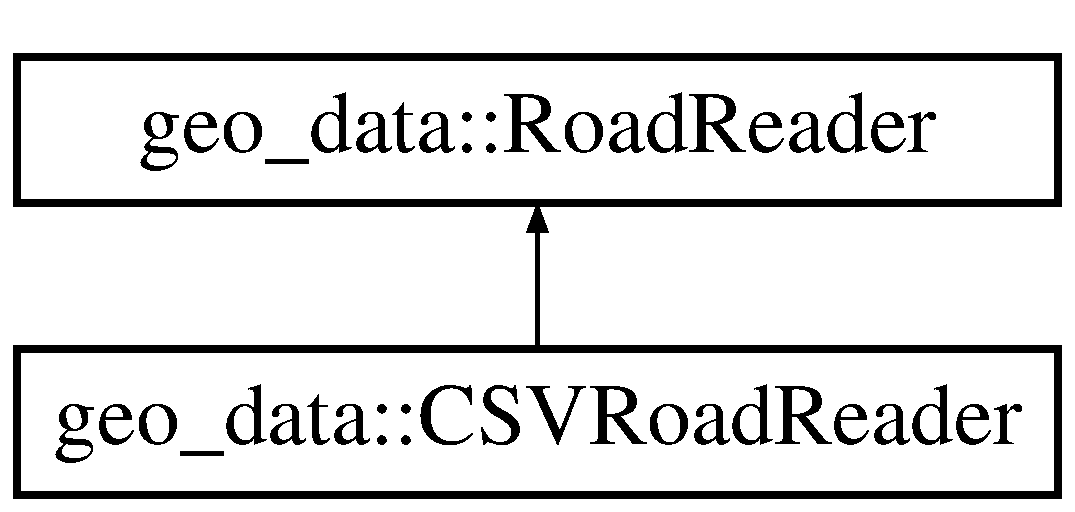
\includegraphics[height=2.000000cm]{classgeo__data_1_1CSVRoadReader}
\end{center}
\end{figure}
\subsection*{Public Member Functions}
\begin{DoxyCompactItemize}
\item 
\hyperlink{classgeo__data_1_1CSVRoadReader_acea18148fa1db97efbade81b780e5312}{C\+S\+V\+Road\+Reader} (const std\+::string \&file\+\_\+path)
\begin{DoxyCompactList}\small\item\em Construct a C\+SV \hyperlink{classgeo__data_1_1RoadReader}{Road\+Reader} object. \end{DoxyCompactList}\item 
\hyperlink{classgeo__data_1_1CSVRoadReader_a3061db500f28034ee2e6faa5bb6a6d45}{$\sim$\+C\+S\+V\+Road\+Reader} ()\hypertarget{classgeo__data_1_1CSVRoadReader_a3061db500f28034ee2e6faa5bb6a6d45}{}\label{classgeo__data_1_1CSVRoadReader_a3061db500f28034ee2e6faa5bb6a6d45}

\begin{DoxyCompactList}\small\item\em Destruct a C\+SV \hyperlink{classgeo__data_1_1RoadReader}{Road\+Reader} object. \end{DoxyCompactList}\item 
geo\+::\+Road\+::\+Ptr \hyperlink{classgeo__data_1_1CSVRoadReader_af926c0827d3fa38fbf26b4557184fecf}{next\+\_\+road} (void)
\begin{DoxyCompactList}\small\item\em Get the next road from the C\+SV file. \end{DoxyCompactList}\end{DoxyCompactItemize}
\subsection*{Additional Inherited Members}


\subsection{Detailed Description}
C\+SV \hyperlink{classgeo__data_1_1RoadReader}{Road\+Reader}. Reads roads from a C\+SV file. 

\subsection{Constructor \& Destructor Documentation}
\index{geo\+\_\+data\+::\+C\+S\+V\+Road\+Reader@{geo\+\_\+data\+::\+C\+S\+V\+Road\+Reader}!C\+S\+V\+Road\+Reader@{C\+S\+V\+Road\+Reader}}
\index{C\+S\+V\+Road\+Reader@{C\+S\+V\+Road\+Reader}!geo\+\_\+data\+::\+C\+S\+V\+Road\+Reader@{geo\+\_\+data\+::\+C\+S\+V\+Road\+Reader}}
\subsubsection[{\texorpdfstring{C\+S\+V\+Road\+Reader(const std\+::string \&file\+\_\+path)}{CSVRoadReader(const std::string &file_path)}}]{\setlength{\rightskip}{0pt plus 5cm}geo\+\_\+data\+::\+C\+S\+V\+Road\+Reader\+::\+C\+S\+V\+Road\+Reader (
\begin{DoxyParamCaption}
\item[{const std\+::string \&}]{file\+\_\+path}
\end{DoxyParamCaption}
)}\hypertarget{classgeo__data_1_1CSVRoadReader_acea18148fa1db97efbade81b780e5312}{}\label{classgeo__data_1_1CSVRoadReader_acea18148fa1db97efbade81b780e5312}


Construct a C\+SV \hyperlink{classgeo__data_1_1RoadReader}{Road\+Reader} object. 


\begin{DoxyParams}{Parameters}
{\em file\+\_\+path} & the C\+SV file \\
\hline
\end{DoxyParams}

\begin{DoxyExceptions}{Exceptions}
{\em std\+::invalid\+\_\+argument} & if the file does not exist or is empty \\
\hline
\end{DoxyExceptions}


\subsection{Member Function Documentation}
\index{geo\+\_\+data\+::\+C\+S\+V\+Road\+Reader@{geo\+\_\+data\+::\+C\+S\+V\+Road\+Reader}!next\+\_\+road@{next\+\_\+road}}
\index{next\+\_\+road@{next\+\_\+road}!geo\+\_\+data\+::\+C\+S\+V\+Road\+Reader@{geo\+\_\+data\+::\+C\+S\+V\+Road\+Reader}}
\subsubsection[{\texorpdfstring{next\+\_\+road(void)}{next_road(void)}}]{\setlength{\rightskip}{0pt plus 5cm}geo\+::\+Road\+::\+Ptr geo\+\_\+data\+::\+C\+S\+V\+Road\+Reader\+::next\+\_\+road (
\begin{DoxyParamCaption}
\item[{void}]{}
\end{DoxyParamCaption}
)\hspace{0.3cm}{\ttfamily [virtual]}}\hypertarget{classgeo__data_1_1CSVRoadReader_af926c0827d3fa38fbf26b4557184fecf}{}\label{classgeo__data_1_1CSVRoadReader_af926c0827d3fa38fbf26b4557184fecf}


Get the next road from the C\+SV file. 

\begin{DoxyReturn}{Returns}
a pointer to \hyperlink{classgeo_1_1Road}{geo\+::\+Road} or nullptr if there are no more roads 
\end{DoxyReturn}


Implements \hyperlink{classgeo__data_1_1RoadReader}{geo\+\_\+data\+::\+Road\+Reader}.



The documentation for this class was generated from the following files\+:\begin{DoxyCompactItemize}
\item 
cvdi-\/src/geo-\/data/include/geo\+\_\+data.\+hpp\item 
cvdi-\/src/geo-\/data/src/geo\+\_\+data.\+cpp\end{DoxyCompactItemize}

\hypertarget{classgeo__data_1_1CSVRoadWriter}{}\section{geo\+\_\+data\+:\+:C\+S\+V\+Road\+Writer Class Reference}
\label{classgeo__data_1_1CSVRoadWriter}\index{geo\+\_\+data\+::\+C\+S\+V\+Road\+Writer@{geo\+\_\+data\+::\+C\+S\+V\+Road\+Writer}}


A C\+SV Road\+Writer. Write roads to a C\+SV file. Overwrites the existing file.  




{\ttfamily \#include $<$geo\+\_\+data.\+hpp$>$}

\subsection*{Public Member Functions}
\begin{DoxyCompactItemize}
\item 
\hyperlink{classgeo__data_1_1CSVRoadWriter_aa36a5283c056925a9f3dd858a39233a2}{C\+S\+V\+Road\+Writer} (const std\+::string \&file\+\_\+path)
\begin{DoxyCompactList}\small\item\em Construct a C\+SV Road\+Writer object. \end{DoxyCompactList}\item 
\hyperlink{classgeo__data_1_1CSVRoadWriter_aa3805df6c1fe6448580af2b57490a87f}{$\sim$\+C\+S\+V\+Road\+Writer} ()\hypertarget{classgeo__data_1_1CSVRoadWriter_aa3805df6c1fe6448580af2b57490a87f}{}\label{classgeo__data_1_1CSVRoadWriter_aa3805df6c1fe6448580af2b57490a87f}

\begin{DoxyCompactList}\small\item\em Destruct a C\+SV Road\+Writer. \end{DoxyCompactList}\item 
void \hyperlink{classgeo__data_1_1CSVRoadWriter_a3b25f08452bd54c267ca53bc5abde1ec}{write\+\_\+road} (\hyperlink{classgeo_1_1Road}{geo\+::\+Road} \&road)\hypertarget{classgeo__data_1_1CSVRoadWriter_a3b25f08452bd54c267ca53bc5abde1ec}{}\label{classgeo__data_1_1CSVRoadWriter_a3b25f08452bd54c267ca53bc5abde1ec}

\begin{DoxyCompactList}\small\item\em Write a road to the C\+SV file. \end{DoxyCompactList}\end{DoxyCompactItemize}


\subsection{Detailed Description}
A C\+SV Road\+Writer. Write roads to a C\+SV file. Overwrites the existing file. 

\subsection{Constructor \& Destructor Documentation}
\index{geo\+\_\+data\+::\+C\+S\+V\+Road\+Writer@{geo\+\_\+data\+::\+C\+S\+V\+Road\+Writer}!C\+S\+V\+Road\+Writer@{C\+S\+V\+Road\+Writer}}
\index{C\+S\+V\+Road\+Writer@{C\+S\+V\+Road\+Writer}!geo\+\_\+data\+::\+C\+S\+V\+Road\+Writer@{geo\+\_\+data\+::\+C\+S\+V\+Road\+Writer}}
\subsubsection[{\texorpdfstring{C\+S\+V\+Road\+Writer(const std\+::string \&file\+\_\+path)}{CSVRoadWriter(const std::string &file_path)}}]{\setlength{\rightskip}{0pt plus 5cm}geo\+\_\+data\+::\+C\+S\+V\+Road\+Writer\+::\+C\+S\+V\+Road\+Writer (
\begin{DoxyParamCaption}
\item[{const std\+::string \&}]{file\+\_\+path}
\end{DoxyParamCaption}
)}\hypertarget{classgeo__data_1_1CSVRoadWriter_aa36a5283c056925a9f3dd858a39233a2}{}\label{classgeo__data_1_1CSVRoadWriter_aa36a5283c056925a9f3dd858a39233a2}


Construct a C\+SV Road\+Writer object. 


\begin{DoxyParams}{Parameters}
{\em file\+\_\+path} & the C\+SV file \\
\hline
\end{DoxyParams}

\begin{DoxyExceptions}{Exceptions}
{\em std\+::invalid\+\_\+argument} & if the file can not be opened \\
\hline
\end{DoxyExceptions}


The documentation for this class was generated from the following files\+:\begin{DoxyCompactItemize}
\item 
cvdi-\/src/geo-\/data/include/geo\+\_\+data.\+hpp\item 
cvdi-\/src/geo-\/data/src/geo\+\_\+data.\+cpp\end{DoxyCompactItemize}

\hypertarget{structfmt_1_1internal_1_1Value_1_1CustomValue}{}\section{fmt\+:\+:internal\+:\+:Value\+:\+:Custom\+Value Struct Reference}
\label{structfmt_1_1internal_1_1Value_1_1CustomValue}\index{fmt\+::internal\+::\+Value\+::\+Custom\+Value@{fmt\+::internal\+::\+Value\+::\+Custom\+Value}}
\subsection*{Public Attributes}
\begin{DoxyCompactItemize}
\item 
const void $\ast$ {\bfseries value}\hypertarget{structfmt_1_1internal_1_1Value_1_1CustomValue_aaaa7c10023f8b3886bee9593cddea150}{}\label{structfmt_1_1internal_1_1Value_1_1CustomValue_aaaa7c10023f8b3886bee9593cddea150}

\item 
Format\+Func {\bfseries format}\hypertarget{structfmt_1_1internal_1_1Value_1_1CustomValue_a36f27ca0939e90a5fe6d7d355ea0f97a}{}\label{structfmt_1_1internal_1_1Value_1_1CustomValue_a36f27ca0939e90a5fe6d7d355ea0f97a}

\end{DoxyCompactItemize}


The documentation for this struct was generated from the following file\+:\begin{DoxyCompactItemize}
\item 
cvdi-\/src/cvdi-\/cl/include/spdlog/fmt/bundled/format.\+h\end{DoxyCompactItemize}

\hypertarget{classcvdi__multi_1_1CVDIParallel}{}\section{cvdi\+\_\+multi\+:\+:C\+V\+D\+I\+Parallel Class Reference}
\label{classcvdi__multi_1_1CVDIParallel}\index{cvdi\+\_\+multi\+::\+C\+V\+D\+I\+Parallel@{cvdi\+\_\+multi\+::\+C\+V\+D\+I\+Parallel}}


Single file C\+V\+DI batch processing application.  




{\ttfamily \#include $<$cvdi\+\_\+multi.\+hpp$>$}

Inheritance diagram for cvdi\+\_\+multi\+:\+:C\+V\+D\+I\+Parallel\+:\begin{figure}[H]
\begin{center}
\leavevmode
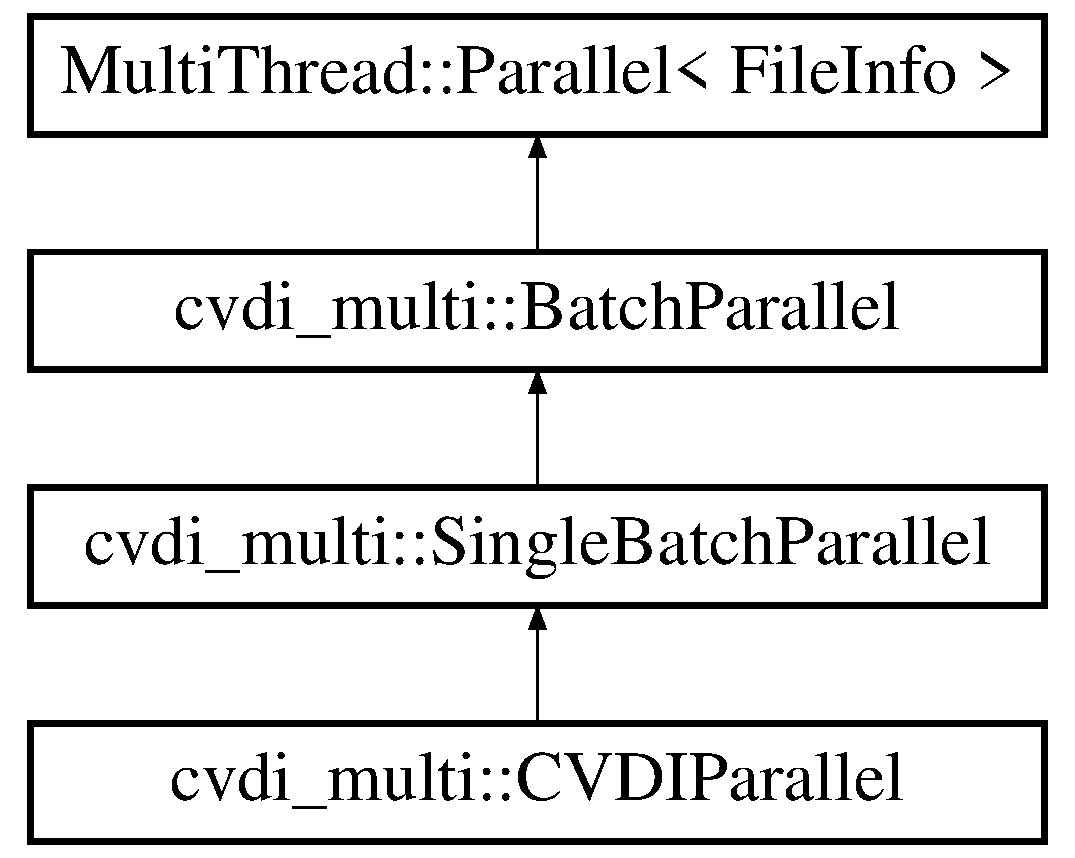
\includegraphics[height=4.000000cm]{classcvdi__multi_1_1CVDIParallel}
\end{center}
\end{figure}
\subsection*{Public Member Functions}
\begin{DoxyCompactItemize}
\item 
{\bfseries C\+V\+D\+I\+Parallel} (const std\+::string file\+\_\+path, const std\+::string osm\+\_\+file, const std\+::string out\+\_\+dir, const std\+::string config\+\_\+file)\hypertarget{classcvdi__multi_1_1CVDIParallel_a7548d213ef13ea2be4634c4d71ee8e49}{}\label{classcvdi__multi_1_1CVDIParallel_a7548d213ef13ea2be4634c4d71ee8e49}

\item 
void \hyperlink{classcvdi__multi_1_1CVDIParallel_a5d162d98140883424d43acd01c562507}{Init} (unsigned n\+\_\+used\+\_\+threads)
\begin{DoxyCompactList}\small\item\em an initialization method; override to perform a concrete initialization action. \end{DoxyCompactList}\item 
void \hyperlink{classcvdi__multi_1_1CVDIParallel_a621f66bf0446ed9a9a63e9fbfb465f1e}{Close} (void)\hypertarget{classcvdi__multi_1_1CVDIParallel_a621f66bf0446ed9a9a63e9fbfb465f1e}{}\label{classcvdi__multi_1_1CVDIParallel_a621f66bf0446ed9a9a63e9fbfb465f1e}

\begin{DoxyCompactList}\small\item\em Close the batch file. \end{DoxyCompactList}\item 
void \hyperlink{classcvdi__multi_1_1CVDIParallel_a7c256d91bb868873a1c6ce854c923c17}{Thread} (unsigned thread\+\_\+num, \hyperlink{classMultiThread_1_1SharedQueue}{Multi\+Thread\+::\+Shared\+Queue}$<$ File\+Info\+::\+Ptr $>$ $\ast$q)
\begin{DoxyCompactList}\small\item\em The main work thread. \end{DoxyCompactList}\end{DoxyCompactItemize}


\subsection{Detailed Description}
Single file C\+V\+DI batch processing application. 

\subsection{Member Function Documentation}
\index{cvdi\+\_\+multi\+::\+C\+V\+D\+I\+Parallel@{cvdi\+\_\+multi\+::\+C\+V\+D\+I\+Parallel}!Init@{Init}}
\index{Init@{Init}!cvdi\+\_\+multi\+::\+C\+V\+D\+I\+Parallel@{cvdi\+\_\+multi\+::\+C\+V\+D\+I\+Parallel}}
\subsubsection[{\texorpdfstring{Init(unsigned n\+\_\+used\+\_\+threads)}{Init(unsigned n_used_threads)}}]{\setlength{\rightskip}{0pt plus 5cm}void cvdi\+\_\+multi\+::\+C\+V\+D\+I\+Parallel\+::\+Init (
\begin{DoxyParamCaption}
\item[{unsigned}]{n\+\_\+used\+\_\+threads}
\end{DoxyParamCaption}
)\hspace{0.3cm}{\ttfamily [virtual]}}\hypertarget{classcvdi__multi_1_1CVDIParallel_a5d162d98140883424d43acd01c562507}{}\label{classcvdi__multi_1_1CVDIParallel_a5d162d98140883424d43acd01c562507}


an initialization method; override to perform a concrete initialization action. 


\begin{DoxyParams}{Parameters}
{\em n\+\_\+used\+\_\+threads} & the number of threads that will be managed by this instance. \\
\hline
\end{DoxyParams}


Reimplemented from \hyperlink{classcvdi__multi_1_1BatchParallel_a40f083a185b29a90733ada3fe789ada2}{cvdi\+\_\+multi\+::\+Batch\+Parallel}.

\index{cvdi\+\_\+multi\+::\+C\+V\+D\+I\+Parallel@{cvdi\+\_\+multi\+::\+C\+V\+D\+I\+Parallel}!Thread@{Thread}}
\index{Thread@{Thread}!cvdi\+\_\+multi\+::\+C\+V\+D\+I\+Parallel@{cvdi\+\_\+multi\+::\+C\+V\+D\+I\+Parallel}}
\subsubsection[{\texorpdfstring{Thread(unsigned thread\+\_\+num, Multi\+Thread\+::\+Shared\+Queue$<$ File\+Info\+::\+Ptr $>$ $\ast$q)}{Thread(unsigned thread_num, MultiThread::SharedQueue< FileInfo::Ptr > *q)}}]{\setlength{\rightskip}{0pt plus 5cm}void cvdi\+\_\+multi\+::\+C\+V\+D\+I\+Parallel\+::\+Thread (
\begin{DoxyParamCaption}
\item[{unsigned}]{thread\+\_\+num, }
\item[{{\bf Multi\+Thread\+::\+Shared\+Queue}$<$ File\+Info\+::\+Ptr $>$ $\ast$}]{q}
\end{DoxyParamCaption}
)\hspace{0.3cm}{\ttfamily [virtual]}}\hypertarget{classcvdi__multi_1_1CVDIParallel_a7c256d91bb868873a1c6ce854c923c17}{}\label{classcvdi__multi_1_1CVDIParallel_a7c256d91bb868873a1c6ce854c923c17}


The main work thread. 


\begin{DoxyParams}{Parameters}
{\em thread\+\_\+num} & a easy to read unique identifier for this thread. \\
\hline
{\em the} & work queue containing the trip files that this thread should process. \\
\hline
\end{DoxyParams}


Implements \hyperlink{classcvdi__multi_1_1SingleBatchParallel_a6514a89e14f2724ab671ffd65d7c43c7}{cvdi\+\_\+multi\+::\+Single\+Batch\+Parallel}.



The documentation for this class was generated from the following files\+:\begin{DoxyCompactItemize}
\item 
cvdi-\/src/cvdi-\/cl/include/cvdi\+\_\+multi.\+hpp\item 
cvdi-\/src/cvdi-\/cl/src/cvdi\+\_\+multi.\+cpp\end{DoxyCompactItemize}

\hypertarget{structspdlog_1_1sinks_1_1dateonly__daily__file__name__calculator}{}\section{spdlog\+:\+:sinks\+:\+:dateonly\+\_\+daily\+\_\+file\+\_\+name\+\_\+calculator Struct Reference}
\label{structspdlog_1_1sinks_1_1dateonly__daily__file__name__calculator}\index{spdlog\+::sinks\+::dateonly\+\_\+daily\+\_\+file\+\_\+name\+\_\+calculator@{spdlog\+::sinks\+::dateonly\+\_\+daily\+\_\+file\+\_\+name\+\_\+calculator}}
\subsection*{Static Public Member Functions}
\begin{DoxyCompactItemize}
\item 
static filename\+\_\+t {\bfseries calc\+\_\+filename} (const filename\+\_\+t \&basename)\hypertarget{structspdlog_1_1sinks_1_1dateonly__daily__file__name__calculator_a2af5b2881a92a50c53dfccb2f180163d}{}\label{structspdlog_1_1sinks_1_1dateonly__daily__file__name__calculator_a2af5b2881a92a50c53dfccb2f180163d}

\end{DoxyCompactItemize}


The documentation for this struct was generated from the following file\+:\begin{DoxyCompactItemize}
\item 
cvdi-\/src/cvdi-\/cl/include/spdlog/sinks/file\+\_\+sinks.\+h\end{DoxyCompactItemize}

\hypertarget{structspdlog_1_1sinks_1_1default__daily__file__name__calculator}{}\section{spdlog\+:\+:sinks\+:\+:default\+\_\+daily\+\_\+file\+\_\+name\+\_\+calculator Struct Reference}
\label{structspdlog_1_1sinks_1_1default__daily__file__name__calculator}\index{spdlog\+::sinks\+::default\+\_\+daily\+\_\+file\+\_\+name\+\_\+calculator@{spdlog\+::sinks\+::default\+\_\+daily\+\_\+file\+\_\+name\+\_\+calculator}}
\subsection*{Static Public Member Functions}
\begin{DoxyCompactItemize}
\item 
static filename\+\_\+t {\bfseries calc\+\_\+filename} (const filename\+\_\+t \&basename)\hypertarget{structspdlog_1_1sinks_1_1default__daily__file__name__calculator_ae2428648ba995d443cd514a3eef071ea}{}\label{structspdlog_1_1sinks_1_1default__daily__file__name__calculator_ae2428648ba995d443cd514a3eef071ea}

\end{DoxyCompactItemize}


The documentation for this struct was generated from the following file\+:\begin{DoxyCompactItemize}
\item 
cvdi-\/src/cvdi-\/cl/include/spdlog/sinks/file\+\_\+sinks.\+h\end{DoxyCompactItemize}

\hypertarget{classcvdi_1_1Stop_1_1Deque}{}\section{cvdi\+:\+:Stop\+:\+:Deque Class Reference}
\label{classcvdi_1_1Stop_1_1Deque}\index{cvdi\+::\+Stop\+::\+Deque@{cvdi\+::\+Stop\+::\+Deque}}


A special deque with support for detecting stops in trace.  




{\ttfamily \#include $<$cvdi.\+hpp$>$}

\subsection*{Public Types}
\begin{DoxyCompactItemize}
\item 
using {\bfseries size\+\_\+type} = std\+::deque$<$ geo\+\_\+data\+::\+Sample\+::\+Trace\+::const\+\_\+iterator $>$\+::size\+\_\+type\hypertarget{classcvdi_1_1Stop_1_1Deque_ab87d53f81657062dd9b54aa9b6ef5664}{}\label{classcvdi_1_1Stop_1_1Deque_ab87d53f81657062dd9b54aa9b6ef5664}

\end{DoxyCompactItemize}
\subsection*{Public Member Functions}
\begin{DoxyCompactItemize}
\item 
\hyperlink{classcvdi_1_1Stop_1_1Deque_a82db9db1295a1d0470e5a2ae5fdceab1}{Deque} (\hyperlink{classcvdi_1_1Stop}{Stop} \&detector)
\begin{DoxyCompactList}\small\item\em Construct a \hyperlink{classcvdi_1_1Stop}{Stop} \hyperlink{classcvdi_1_1Stop_1_1Deque}{Deque} object. \end{DoxyCompactList}\item 
double \hyperlink{classcvdi_1_1Stop_1_1Deque_af2be913dfab359504aaebc7620d7399b}{delta\+\_\+distance} () const 
\begin{DoxyCompactList}\small\item\em Get the point-\/to-\/point distance in meters covered by points in the \hyperlink{classcvdi_1_1Stop}{Stop} \hyperlink{classcvdi_1_1Stop_1_1Deque}{Deque}. \end{DoxyCompactList}\item 
double \hyperlink{classcvdi_1_1Stop_1_1Deque_ae6b2b3fccac30fe6112ff6da6aafcd90}{cover\+\_\+distance} () const 
\begin{DoxyCompactList}\small\item\em Get the distance between the first point and last point in the \hyperlink{classcvdi_1_1Stop}{Stop} \hyperlink{classcvdi_1_1Stop_1_1Deque}{Deque}. \end{DoxyCompactList}\item 
void \hyperlink{classcvdi_1_1Stop_1_1Deque_ad277103300d4fc3a09afbe0b575a4567}{push\+\_\+right} (const geo\+\_\+data\+::\+Sample\+::\+Trace\+::const\+\_\+iterator \&it)
\begin{DoxyCompactList}\small\item\em Add a point (iterator) to the back (right) of the deque and update the point-\/to-\/point distance. \end{DoxyCompactList}\item 
bool \hyperlink{classcvdi_1_1Stop_1_1Deque_aab0122a2992c126d1ccc9e6b5dfd04f9}{unwind} ()
\begin{DoxyCompactList}\small\item\em Remove iterators (points) from the front of the deque until the following conditions are met\+: \end{DoxyCompactList}\item 
void \hyperlink{classcvdi_1_1Stop_1_1Deque_a07479bd54399d00d977965de4608f57d}{reset} ()\hypertarget{classcvdi_1_1Stop_1_1Deque_a07479bd54399d00d977965de4608f57d}{}\label{classcvdi_1_1Stop_1_1Deque_a07479bd54399d00d977965de4608f57d}

\begin{DoxyCompactList}\small\item\em Reset this \hyperlink{classcvdi_1_1Stop}{Stop} \hyperlink{classcvdi_1_1Stop_1_1Deque}{Deque} instance. Remove all points (iterators) from the deque and reset cumulated distance to 0. \end{DoxyCompactList}\item 
bool \hyperlink{classcvdi_1_1Stop_1_1Deque_a4e267019ceae75025ac0aadc4c073a28}{under\+\_\+time} (geo\+\_\+data\+::\+Sample\+::\+Ptr sample) const 
\begin{DoxyCompactList}\small\item\em Predicate indicating whether the time elapsed from the first trip point in the deque to this trip point does not exceed max\+\_\+time. \end{DoxyCompactList}\item 
bool \hyperlink{classcvdi_1_1Stop_1_1Deque_a891bee58957586879e58a34ef4839c3e}{under\+\_\+distance} () const 
\begin{DoxyCompactList}\small\item\em Predicate indicating whether the distance covered by the points in the deque is less than the parameterized limit. \end{DoxyCompactList}\item 
bool \hyperlink{classcvdi_1_1Stop_1_1Deque_a26a9eef47ae371704ec54b4442c0649b}{under\+\_\+speed} (geo\+\_\+data\+::\+Sample\+::\+Ptr sample) const 
\begin{DoxyCompactList}\small\item\em Predicate that indicates the speed in this point record is less than the limit. \end{DoxyCompactList}\end{DoxyCompactItemize}
\subsection*{Friends}
\begin{DoxyCompactItemize}
\item 
class {\bfseries Stop}\hypertarget{classcvdi_1_1Stop_1_1Deque_a06c1356535b989762bfdfc0f8fcc76ae}{}\label{classcvdi_1_1Stop_1_1Deque_a06c1356535b989762bfdfc0f8fcc76ae}

\item 
std\+::ostream \& \hyperlink{classcvdi_1_1Stop_1_1Deque_a573b40bf9fa3ab3485f1a8335d1dac7c}{operator$<$$<$} (std\+::ostream \&os, const \hyperlink{classcvdi_1_1Stop_1_1Deque}{Deque} \&q)
\begin{DoxyCompactList}\small\item\em Output to a stream details about this \hyperlink{classcvdi_1_1Stop}{Stop} \hyperlink{classcvdi_1_1Stop_1_1Deque}{Deque}. \end{DoxyCompactList}\end{DoxyCompactItemize}


\subsection{Detailed Description}
A special deque with support for detecting stops in trace. 

\subsection{Constructor \& Destructor Documentation}
\index{cvdi\+::\+Stop\+::\+Deque@{cvdi\+::\+Stop\+::\+Deque}!Deque@{Deque}}
\index{Deque@{Deque}!cvdi\+::\+Stop\+::\+Deque@{cvdi\+::\+Stop\+::\+Deque}}
\subsubsection[{\texorpdfstring{Deque(\+Stop \&detector)}{Deque(Stop &detector)}}]{\setlength{\rightskip}{0pt plus 5cm}cvdi\+::\+Stop\+::\+Deque\+::\+Deque (
\begin{DoxyParamCaption}
\item[{{\bf Stop} \&}]{detector}
\end{DoxyParamCaption}
)}\hypertarget{classcvdi_1_1Stop_1_1Deque_a82db9db1295a1d0470e5a2ae5fdceab1}{}\label{classcvdi_1_1Stop_1_1Deque_a82db9db1295a1d0470e5a2ae5fdceab1}


Construct a \hyperlink{classcvdi_1_1Stop}{Stop} \hyperlink{classcvdi_1_1Stop_1_1Deque}{Deque} object. 


\begin{DoxyParams}{Parameters}
{\em detector} & a reference to the \hyperlink{classcvdi_1_1Stop}{Stop} instance to support\\
\hline
\end{DoxyParams}
C\+T\+OR for new stop detector deque. 

\subsection{Member Function Documentation}
\index{cvdi\+::\+Stop\+::\+Deque@{cvdi\+::\+Stop\+::\+Deque}!cover\+\_\+distance@{cover\+\_\+distance}}
\index{cover\+\_\+distance@{cover\+\_\+distance}!cvdi\+::\+Stop\+::\+Deque@{cvdi\+::\+Stop\+::\+Deque}}
\subsubsection[{\texorpdfstring{cover\+\_\+distance() const }{cover_distance() const }}]{\setlength{\rightskip}{0pt plus 5cm}double cvdi\+::\+Stop\+::\+Deque\+::cover\+\_\+distance (
\begin{DoxyParamCaption}
{}
\end{DoxyParamCaption}
) const}\hypertarget{classcvdi_1_1Stop_1_1Deque_ae6b2b3fccac30fe6112ff6da6aafcd90}{}\label{classcvdi_1_1Stop_1_1Deque_ae6b2b3fccac30fe6112ff6da6aafcd90}


Get the distance between the first point and last point in the \hyperlink{classcvdi_1_1Stop}{Stop} \hyperlink{classcvdi_1_1Stop_1_1Deque}{Deque}. 

\begin{DoxyReturn}{Returns}
the distance in meters
\end{DoxyReturn}
The direct distance from first point to last point within the deque.

N\+O\+TE\+: This seems to be a better metric because G\+PS error could infer a larger manhattan distance when a vehicle is actually not moving at all. \index{cvdi\+::\+Stop\+::\+Deque@{cvdi\+::\+Stop\+::\+Deque}!delta\+\_\+distance@{delta\+\_\+distance}}
\index{delta\+\_\+distance@{delta\+\_\+distance}!cvdi\+::\+Stop\+::\+Deque@{cvdi\+::\+Stop\+::\+Deque}}
\subsubsection[{\texorpdfstring{delta\+\_\+distance() const }{delta_distance() const }}]{\setlength{\rightskip}{0pt plus 5cm}double cvdi\+::\+Stop\+::\+Deque\+::delta\+\_\+distance (
\begin{DoxyParamCaption}
{}
\end{DoxyParamCaption}
) const}\hypertarget{classcvdi_1_1Stop_1_1Deque_af2be913dfab359504aaebc7620d7399b}{}\label{classcvdi_1_1Stop_1_1Deque_af2be913dfab359504aaebc7620d7399b}


Get the point-\/to-\/point distance in meters covered by points in the \hyperlink{classcvdi_1_1Stop}{Stop} \hyperlink{classcvdi_1_1Stop_1_1Deque}{Deque}. 

\begin{DoxyReturn}{Returns}
the distance in meters
\end{DoxyReturn}
The manhattan distance covered by the points within the deque. \index{cvdi\+::\+Stop\+::\+Deque@{cvdi\+::\+Stop\+::\+Deque}!push\+\_\+right@{push\+\_\+right}}
\index{push\+\_\+right@{push\+\_\+right}!cvdi\+::\+Stop\+::\+Deque@{cvdi\+::\+Stop\+::\+Deque}}
\subsubsection[{\texorpdfstring{push\+\_\+right(const geo\+\_\+data\+::\+Sample\+::\+Trace\+::const\+\_\+iterator \&it)}{push_right(const geo_data::Sample::Trace::const_iterator &it)}}]{\setlength{\rightskip}{0pt plus 5cm}void cvdi\+::\+Stop\+::\+Deque\+::push\+\_\+right (
\begin{DoxyParamCaption}
\item[{const geo\+\_\+data\+::\+Sample\+::\+Trace\+::const\+\_\+iterator \&}]{it}
\end{DoxyParamCaption}
)}\hypertarget{classcvdi_1_1Stop_1_1Deque_ad277103300d4fc3a09afbe0b575a4567}{}\label{classcvdi_1_1Stop_1_1Deque_ad277103300d4fc3a09afbe0b575a4567}


Add a point (iterator) to the back (right) of the deque and update the point-\/to-\/point distance. 


\begin{DoxyParams}{Parameters}
{\em it} & An iterator to a trace point\\
\hline
\end{DoxyParams}
Add a point/iterator to the back (right) of the deque and update the manhattan distance. \index{cvdi\+::\+Stop\+::\+Deque@{cvdi\+::\+Stop\+::\+Deque}!under\+\_\+distance@{under\+\_\+distance}}
\index{under\+\_\+distance@{under\+\_\+distance}!cvdi\+::\+Stop\+::\+Deque@{cvdi\+::\+Stop\+::\+Deque}}
\subsubsection[{\texorpdfstring{under\+\_\+distance() const }{under_distance() const }}]{\setlength{\rightskip}{0pt plus 5cm}bool cvdi\+::\+Stop\+::\+Deque\+::under\+\_\+distance (
\begin{DoxyParamCaption}
{}
\end{DoxyParamCaption}
) const}\hypertarget{classcvdi_1_1Stop_1_1Deque_a891bee58957586879e58a34ef4839c3e}{}\label{classcvdi_1_1Stop_1_1Deque_a891bee58957586879e58a34ef4839c3e}


Predicate indicating whether the distance covered by the points in the deque is less than the parameterized limit. 

Cover distance is used since G\+PS error can greatly skew the Manhattan distance in instances where no actual movement has taken place. In cases where the driver is traveling in a straight line, both cover\+\_\+distance and Manhattan distance will be equivalent.

\begin{DoxyReturn}{Returns}
true if cover distance $<$= limit, false otherwise.
\end{DoxyReturn}
Prediate indicating whether the distance covered by the points in the deque is less than the limit at which too much movement has taken place to consider it a stop.

Cover distance is used since G\+PS error can greatly skew the manhattan distance in instances where no actual movement has taken place. In cases where the driver is traveling in a straight line, both cover\+\_\+distance and manhattan distance will be equivalent. \index{cvdi\+::\+Stop\+::\+Deque@{cvdi\+::\+Stop\+::\+Deque}!under\+\_\+speed@{under\+\_\+speed}}
\index{under\+\_\+speed@{under\+\_\+speed}!cvdi\+::\+Stop\+::\+Deque@{cvdi\+::\+Stop\+::\+Deque}}
\subsubsection[{\texorpdfstring{under\+\_\+speed(geo\+\_\+data\+::\+Sample\+::\+Ptr sample) const }{under_speed(geo_data::Sample::Ptr sample) const }}]{\setlength{\rightskip}{0pt plus 5cm}bool cvdi\+::\+Stop\+::\+Deque\+::under\+\_\+speed (
\begin{DoxyParamCaption}
\item[{geo\+\_\+data\+::\+Sample\+::\+Ptr}]{ptptr}
\end{DoxyParamCaption}
) const}\hypertarget{classcvdi_1_1Stop_1_1Deque_a26a9eef47ae371704ec54b4442c0649b}{}\label{classcvdi_1_1Stop_1_1Deque_a26a9eef47ae371704ec54b4442c0649b}


Predicate that indicates the speed in this point record is less than the limit. 

Points having speeds greater than or equal to this speed are not considered by the stop detector.


\begin{DoxyParams}{Parameters}
{\em sample} & sample point in a trace \\
\hline
\end{DoxyParams}
\begin{DoxyReturn}{Returns}
true if the points current speeds is less than the parameterized max speed.
\end{DoxyReturn}
Predicate that indicates the speed in this point record is less than the speed where we start considering (collecting points) stop detection properties. \index{cvdi\+::\+Stop\+::\+Deque@{cvdi\+::\+Stop\+::\+Deque}!under\+\_\+time@{under\+\_\+time}}
\index{under\+\_\+time@{under\+\_\+time}!cvdi\+::\+Stop\+::\+Deque@{cvdi\+::\+Stop\+::\+Deque}}
\subsubsection[{\texorpdfstring{under\+\_\+time(geo\+\_\+data\+::\+Sample\+::\+Ptr sample) const }{under_time(geo_data::Sample::Ptr sample) const }}]{\setlength{\rightskip}{0pt plus 5cm}bool cvdi\+::\+Stop\+::\+Deque\+::under\+\_\+time (
\begin{DoxyParamCaption}
\item[{geo\+\_\+data\+::\+Sample\+::\+Ptr}]{ptptr}
\end{DoxyParamCaption}
) const}\hypertarget{classcvdi_1_1Stop_1_1Deque_a4e267019ceae75025ac0aadc4c073a28}{}\label{classcvdi_1_1Stop_1_1Deque_a4e267019ceae75025ac0aadc4c073a28}


Predicate indicating whether the time elapsed from the first trip point in the deque to this trip point does not exceed max\+\_\+time. 


\begin{DoxyParams}{Parameters}
{\em sample} & a point in a trace; this point is later in the trip than the first point in the deque.\\
\hline
\end{DoxyParams}
\begin{DoxyReturn}{Returns}
true if the time difference is less than or equal to the max\+\_\+time.
\end{DoxyReturn}
Predicate indicating whether the deque\textquotesingle{}s I\+N\+V\+A\+R\+I\+A\+NT would be broken by adding this trip point to it.

I\+N\+V\+A\+R\+I\+A\+NT\+: The time elapsed from first trip point in deque to last never exceeds max\+\_\+time. \index{cvdi\+::\+Stop\+::\+Deque@{cvdi\+::\+Stop\+::\+Deque}!unwind@{unwind}}
\index{unwind@{unwind}!cvdi\+::\+Stop\+::\+Deque@{cvdi\+::\+Stop\+::\+Deque}}
\subsubsection[{\texorpdfstring{unwind()}{unwind()}}]{\setlength{\rightskip}{0pt plus 5cm}bool cvdi\+::\+Stop\+::\+Deque\+::unwind (
\begin{DoxyParamCaption}
{}
\end{DoxyParamCaption}
)}\hypertarget{classcvdi_1_1Stop_1_1Deque_aab0122a2992c126d1ccc9e6b5dfd04f9}{}\label{classcvdi_1_1Stop_1_1Deque_aab0122a2992c126d1ccc9e6b5dfd04f9}


Remove iterators (points) from the front of the deque until the following conditions are met\+: 


\begin{DoxyEnumerate}
\item The distance covered in the deque is under the limit.
\item The deque does not become empty.
\item The velocity is below the limit and the road is not in the blacklist.
\end{DoxyEnumerate}

\begin{DoxyReturn}{Returns}
true if the deque is empty (stop condition); false if it is not empty
\end{DoxyReturn}
Remove iterators (points) from the front of the deque until the following conditions are met\+:


\begin{DoxyEnumerate}
\item The distance covered in the deque is under the limit.
\item The deque does not become empty.
\item The velocity is below the limit and the road is not in the blacklist.
\end{DoxyEnumerate}

Return\+: true if the deque is empty (stop condition); false if it is not empty. 

\subsection{Friends And Related Function Documentation}
\index{cvdi\+::\+Stop\+::\+Deque@{cvdi\+::\+Stop\+::\+Deque}!operator$<$$<$@{operator$<$$<$}}
\index{operator$<$$<$@{operator$<$$<$}!cvdi\+::\+Stop\+::\+Deque@{cvdi\+::\+Stop\+::\+Deque}}
\subsubsection[{\texorpdfstring{operator$<$$<$}{operator<<}}]{\setlength{\rightskip}{0pt plus 5cm}std\+::ostream\& operator$<$$<$ (
\begin{DoxyParamCaption}
\item[{std\+::ostream \&}]{os, }
\item[{const {\bf Deque} \&}]{q}
\end{DoxyParamCaption}
)\hspace{0.3cm}{\ttfamily [friend]}}\hypertarget{classcvdi_1_1Stop_1_1Deque_a573b40bf9fa3ab3485f1a8335d1dac7c}{}\label{classcvdi_1_1Stop_1_1Deque_a573b40bf9fa3ab3485f1a8335d1dac7c}


Output to a stream details about this \hyperlink{classcvdi_1_1Stop}{Stop} \hyperlink{classcvdi_1_1Stop_1_1Deque}{Deque}. 


\begin{DoxyParams}{Parameters}
{\em os} & the output stream \\
\hline
{\em q} & the \hyperlink{classcvdi_1_1Stop}{Stop} \hyperlink{classcvdi_1_1Stop_1_1Deque}{Deque} \\
\hline
\end{DoxyParams}
\begin{DoxyReturn}{Returns}
the output stream after printing for chaining 
\end{DoxyReturn}


The documentation for this class was generated from the following files\+:\begin{DoxyCompactItemize}
\item 
cvdi-\/src/cvdi/include/cvdi.\+hpp\item 
cvdi-\/src/cvdi/src/cvdi.\+cpp\end{DoxyCompactItemize}

\hypertarget{classspdlog_1_1sinks_1_1dist__sink}{}\section{spdlog\+:\+:sinks\+:\+:dist\+\_\+sink$<$ Mutex $>$ Class Template Reference}
\label{classspdlog_1_1sinks_1_1dist__sink}\index{spdlog\+::sinks\+::dist\+\_\+sink$<$ Mutex $>$@{spdlog\+::sinks\+::dist\+\_\+sink$<$ Mutex $>$}}
Inheritance diagram for spdlog\+:\+:sinks\+:\+:dist\+\_\+sink$<$ Mutex $>$\+:\begin{figure}[H]
\begin{center}
\leavevmode
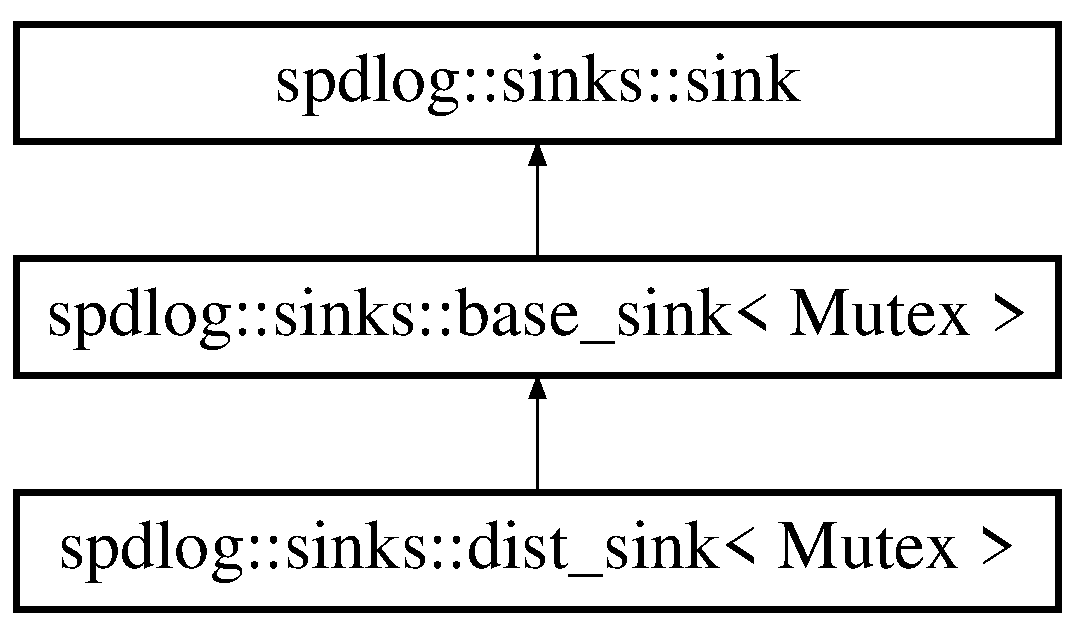
\includegraphics[height=3.000000cm]{classspdlog_1_1sinks_1_1dist__sink}
\end{center}
\end{figure}
\subsection*{Public Member Functions}
\begin{DoxyCompactItemize}
\item 
{\bfseries dist\+\_\+sink} (const \hyperlink{classspdlog_1_1sinks_1_1dist__sink}{dist\+\_\+sink} \&)=delete\hypertarget{classspdlog_1_1sinks_1_1dist__sink_afadef20aeb435c8b62b2efa2f0906de5}{}\label{classspdlog_1_1sinks_1_1dist__sink_afadef20aeb435c8b62b2efa2f0906de5}

\item 
\hyperlink{classspdlog_1_1sinks_1_1dist__sink}{dist\+\_\+sink} \& {\bfseries operator=} (const \hyperlink{classspdlog_1_1sinks_1_1dist__sink}{dist\+\_\+sink} \&)=delete\hypertarget{classspdlog_1_1sinks_1_1dist__sink_a6f91b5522c12fd448ca2fd7cb8fe0097}{}\label{classspdlog_1_1sinks_1_1dist__sink_a6f91b5522c12fd448ca2fd7cb8fe0097}

\item 
void {\bfseries add\+\_\+sink} (std\+::shared\+\_\+ptr$<$ \hyperlink{classspdlog_1_1sinks_1_1sink}{sink} $>$ \hyperlink{classspdlog_1_1sinks_1_1sink}{sink})\hypertarget{classspdlog_1_1sinks_1_1dist__sink_ae2250f59f23ecaf3214da6059198ad3c}{}\label{classspdlog_1_1sinks_1_1dist__sink_ae2250f59f23ecaf3214da6059198ad3c}

\item 
void {\bfseries remove\+\_\+sink} (std\+::shared\+\_\+ptr$<$ \hyperlink{classspdlog_1_1sinks_1_1sink}{sink} $>$ \hyperlink{classspdlog_1_1sinks_1_1sink}{sink})\hypertarget{classspdlog_1_1sinks_1_1dist__sink_ac1537fdc6225fd57cc819e1fb9c5f8c7}{}\label{classspdlog_1_1sinks_1_1dist__sink_ac1537fdc6225fd57cc819e1fb9c5f8c7}

\end{DoxyCompactItemize}
\subsection*{Protected Member Functions}
\begin{DoxyCompactItemize}
\item 
void {\bfseries \+\_\+sink\+\_\+it} (const \hyperlink{structspdlog_1_1details_1_1log__msg}{details\+::log\+\_\+msg} \&msg) override\hypertarget{classspdlog_1_1sinks_1_1dist__sink_a9458a326a60b6c0183c9ff8ce7aca221}{}\label{classspdlog_1_1sinks_1_1dist__sink_a9458a326a60b6c0183c9ff8ce7aca221}

\item 
void {\bfseries \+\_\+flush} () override\hypertarget{classspdlog_1_1sinks_1_1dist__sink_aeaf56b9977a2c2afb262f6aa3b6f065b}{}\label{classspdlog_1_1sinks_1_1dist__sink_aeaf56b9977a2c2afb262f6aa3b6f065b}

\end{DoxyCompactItemize}
\subsection*{Protected Attributes}
\begin{DoxyCompactItemize}
\item 
std\+::vector$<$ std\+::shared\+\_\+ptr$<$ \hyperlink{classspdlog_1_1sinks_1_1sink}{sink} $>$ $>$ {\bfseries \+\_\+sinks}\hypertarget{classspdlog_1_1sinks_1_1dist__sink_a13027b6f399ae33c5e75aa54f4da4e71}{}\label{classspdlog_1_1sinks_1_1dist__sink_a13027b6f399ae33c5e75aa54f4da4e71}

\end{DoxyCompactItemize}


The documentation for this class was generated from the following file\+:\begin{DoxyCompactItemize}
\item 
cvdi-\/src/cvdi-\/cl/include/spdlog/sinks/dist\+\_\+sink.\+h\end{DoxyCompactItemize}

\hypertarget{structfmt_1_1internal_1_1DummyInt}{}\section{fmt\+:\+:internal\+:\+:Dummy\+Int Struct Reference}
\label{structfmt_1_1internal_1_1DummyInt}\index{fmt\+::internal\+::\+Dummy\+Int@{fmt\+::internal\+::\+Dummy\+Int}}
\subsection*{Public Member Functions}
\begin{DoxyCompactItemize}
\item 
{\bfseries operator int} () const \hypertarget{structfmt_1_1internal_1_1DummyInt_a661adc117b3c83ab3aa91aaef0b3bf29}{}\label{structfmt_1_1internal_1_1DummyInt_a661adc117b3c83ab3aa91aaef0b3bf29}

\end{DoxyCompactItemize}
\subsection*{Public Attributes}
\begin{DoxyCompactItemize}
\item 
int {\bfseries data} \mbox{[}2\mbox{]}\hypertarget{structfmt_1_1internal_1_1DummyInt_a0b785da86f9605b7fbebba9014dcfa61}{}\label{structfmt_1_1internal_1_1DummyInt_a0b785da86f9605b7fbebba9014dcfa61}

\end{DoxyCompactItemize}


The documentation for this struct was generated from the following file\+:\begin{DoxyCompactItemize}
\item 
cvdi-\/src/cvdi-\/cl/include/spdlog/fmt/bundled/format.\+h\end{DoxyCompactItemize}

\hypertarget{structfmt_1_1internal_1_1DummyStream}{}\section{fmt\+:\+:internal\+:\+:Dummy\+Stream Struct Reference}
\label{structfmt_1_1internal_1_1DummyStream}\index{fmt\+::internal\+::\+Dummy\+Stream@{fmt\+::internal\+::\+Dummy\+Stream}}
Inheritance diagram for fmt\+:\+:internal\+:\+:Dummy\+Stream\+:\begin{figure}[H]
\begin{center}
\leavevmode
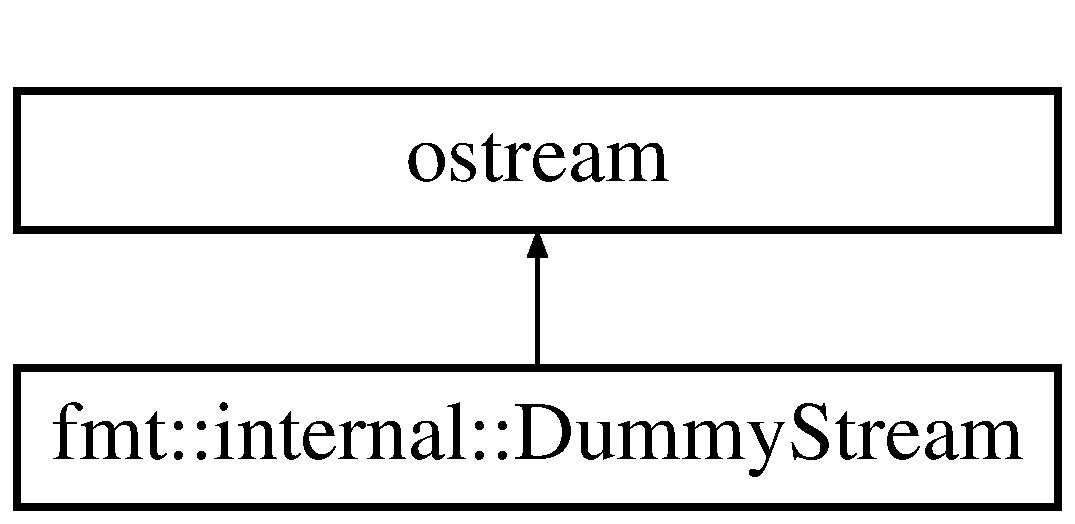
\includegraphics[height=2.000000cm]{structfmt_1_1internal_1_1DummyStream}
\end{center}
\end{figure}
\subsection*{Public Member Functions}
\begin{DoxyCompactItemize}
\item 
void {\bfseries operator$<$$<$} (\hyperlink{structfmt_1_1internal_1_1Null}{Null}$<$$>$)\hypertarget{structfmt_1_1internal_1_1DummyStream_a42f21ef25da7abaa29821b7d5fc4e2d6}{}\label{structfmt_1_1internal_1_1DummyStream_a42f21ef25da7abaa29821b7d5fc4e2d6}

\end{DoxyCompactItemize}


The documentation for this struct was generated from the following file\+:\begin{DoxyCompactItemize}
\item 
cvdi-\/src/cvdi-\/cl/include/spdlog/fmt/bundled/ostream.\+h\end{DoxyCompactItemize}

\hypertarget{classgeo_1_1Edge}{}\section{geo\+:\+:Edge Class Reference}
\label{classgeo_1_1Edge}\index{geo\+::\+Edge@{geo\+::\+Edge}}


\hyperlink{classgeo_1_1Edge}{Edge} class containing a basic line string and meta data associated with the underlying real world road. \hyperlink{classgeo_1_1Edge}{Edge} objects are similar to \hyperlink{classgeo_1_1Road}{Road} objects except that they are one-\/directional and used in the graph topology. Because and edge is part of a topology, each edge will point to a successor edge and possible a neighbor edge.  




{\ttfamily \#include $<$geo.\+hpp$>$}

\subsection*{Public Types}
\begin{DoxyCompactItemize}
\item 
using {\bfseries Ptr} = std\+::shared\+\_\+ptr$<$ \hyperlink{classgeo_1_1Edge}{Edge} $>$\hypertarget{classgeo_1_1Edge_a42cbd37dad3201c3d4386e7e781a260a}{}\label{classgeo_1_1Edge_a42cbd37dad3201c3d4386e7e781a260a}

\end{DoxyCompactItemize}
\subsection*{Public Member Functions}
\begin{DoxyCompactItemize}
\item 
\hyperlink{classgeo_1_1Edge_a0e93626d5bf90f09430535a501ad7850}{Edge} (Road\+::\+Ptr road\+\_\+ptr, \hyperlink{namespacegeo_ae7a495a59f07984a90e0b609bc038df9}{Heading} \hyperlink{classgeo_1_1Edge_a42070020fa7326a102316b7aab57801b}{heading})
\begin{DoxyCompactList}\small\item\em Construct an \hyperlink{classgeo_1_1Edge}{Edge} object from a \hyperlink{classgeo_1_1Road}{Road} object pointer, and heading of the \hyperlink{classgeo_1_1Edge}{Edge}. \end{DoxyCompactList}\item 
\hyperlink{classgeo_1_1Edge_a47b947fe3b87e6a28edf790c83e39fb0}{Edge} (long \hyperlink{classgeo_1_1Edge_a459268032f5d9ccf412b66569f5ac258}{id})\hypertarget{classgeo_1_1Edge_a47b947fe3b87e6a28edf790c83e39fb0}{}\label{classgeo_1_1Edge_a47b947fe3b87e6a28edf790c83e39fb0}

\begin{DoxyCompactList}\small\item\em Construct an abstract \hyperlink{classgeo_1_1Edge}{Edge}. This will create an empty line string, which can be used to build edges that don\textquotesingle{}t represent real world roads. \end{DoxyCompactList}\item 
long \hyperlink{classgeo_1_1Edge_a459268032f5d9ccf412b66569f5ac258}{id} () const 
\begin{DoxyCompactList}\small\item\em Get the unique ID of this edge. \end{DoxyCompactList}\item 
long \hyperlink{classgeo_1_1Edge_a01e03971727a7ee252b64c4a5991aae3}{source} () const 
\begin{DoxyCompactList}\small\item\em Get the ID of the source vertex of this edge. \end{DoxyCompactList}\item 
long \hyperlink{classgeo_1_1Edge_a2710a346c2eec1dc979d529f7067e7c9}{target} () const 
\begin{DoxyCompactList}\small\item\em Get the ID of the target vertex of this edge. \end{DoxyCompactList}\item 
double \hyperlink{classgeo_1_1Edge_a752e5cfb9e469a1523fad88088167874}{length} () const 
\begin{DoxyCompactList}\small\item\em Get the length of this edge in meters. \end{DoxyCompactList}\item 
double \hyperlink{classgeo_1_1Edge_a3f7e577f1218b742a387fe9c23030689}{width} () const 
\begin{DoxyCompactList}\small\item\em Get the approximate width in meters of this edge. \end{DoxyCompactList}\item 
float \hyperlink{classgeo_1_1Edge_a23de2560879285876899961e614fc433}{priority} () const 
\begin{DoxyCompactList}\small\item\em Get the use priority for this edge. \end{DoxyCompactList}\item 
int \hyperlink{classgeo_1_1Edge_ab2913bedb82fd1e24e0c99d5ea6c7a87}{maxspeed} () const 
\begin{DoxyCompactList}\small\item\em Get the maximum speed for this edge as kilometers per hour. \end{DoxyCompactList}\item 
\hyperlink{namespacegeo_ae7a495a59f07984a90e0b609bc038df9}{Heading} \hyperlink{classgeo_1_1Edge_a42070020fa7326a102316b7aab57801b}{heading} () const 
\begin{DoxyCompactList}\small\item\em Get the heading (forward or backward) of this edge. \end{DoxyCompactList}\item 
Ptr \hyperlink{classgeo_1_1Edge_aba1290f592ea2cd848fcb801f0562df2}{successor} () const 
\begin{DoxyCompactList}\small\item\em Get the pointer to the successor edge for this edge. \end{DoxyCompactList}\item 
Ptr \hyperlink{classgeo_1_1Edge_aad32f284aba317162ae6276497926268}{neighbor} () const 
\begin{DoxyCompactList}\small\item\em Get the pointer to the neighbor edge for this edge. \end{DoxyCompactList}\item 
void \hyperlink{classgeo_1_1Edge_a571ee74792a242715887d699a9486e53}{successor} (Ptr successor)
\begin{DoxyCompactList}\small\item\em Set the pointer to the successor edge for this edge. \end{DoxyCompactList}\item 
void \hyperlink{classgeo_1_1Edge_a001d13006bed7403a1ddf920a937bf4e}{neighbor} (Ptr neighbor)
\begin{DoxyCompactList}\small\item\em Set the pointer to the neighbor edge for this edge. \end{DoxyCompactList}\item 
Road\+::\+Ptr \hyperlink{classgeo_1_1Edge_a96fc3fb170d60c5eed77a4fb274f4741}{road} () const \hypertarget{classgeo_1_1Edge_a96fc3fb170d60c5eed77a4fb274f4741}{}\label{classgeo_1_1Edge_a96fc3fb170d60c5eed77a4fb274f4741}

\begin{DoxyCompactList}\small\item\em Get the pointer the base \hyperlink{classgeo_1_1Road}{Road} object for this edge. \end{DoxyCompactList}\item 
long \hyperlink{classgeo_1_1Edge_ad93db783fea4d5017739aba83a973acc}{type} () const 
\begin{DoxyCompactList}\small\item\em Get the O\+SM way type of this edge. \end{DoxyCompactList}\end{DoxyCompactItemize}
\subsection*{Public Attributes}
\begin{DoxyCompactItemize}
\item 
O\+G\+R\+Line\+String \hyperlink{classgeo_1_1Edge_adaca6b6b12347bb7ce47da4e3d1d1c6a}{line\+\_\+string}\hypertarget{classgeo_1_1Edge_adaca6b6b12347bb7ce47da4e3d1d1c6a}{}\label{classgeo_1_1Edge_adaca6b6b12347bb7ce47da4e3d1d1c6a}

\begin{DoxyCompactList}\small\item\em The underlying line string of this edge as an O\+G\+R\+Line\+String. \end{DoxyCompactList}\end{DoxyCompactItemize}


\subsection{Detailed Description}
\hyperlink{classgeo_1_1Edge}{Edge} class containing a basic line string and meta data associated with the underlying real world road. \hyperlink{classgeo_1_1Edge}{Edge} objects are similar to \hyperlink{classgeo_1_1Road}{Road} objects except that they are one-\/directional and used in the graph topology. Because and edge is part of a topology, each edge will point to a successor edge and possible a neighbor edge. 

\subsection{Constructor \& Destructor Documentation}
\index{geo\+::\+Edge@{geo\+::\+Edge}!Edge@{Edge}}
\index{Edge@{Edge}!geo\+::\+Edge@{geo\+::\+Edge}}
\subsubsection[{\texorpdfstring{Edge(\+Road\+::\+Ptr road\+\_\+ptr, Heading heading)}{Edge(Road::Ptr road_ptr, Heading heading)}}]{\setlength{\rightskip}{0pt plus 5cm}geo\+::\+Edge\+::\+Edge (
\begin{DoxyParamCaption}
\item[{Road\+::\+Ptr}]{road\+\_\+ptr, }
\item[{{\bf Heading}}]{heading}
\end{DoxyParamCaption}
)}\hypertarget{classgeo_1_1Edge_a0e93626d5bf90f09430535a501ad7850}{}\label{classgeo_1_1Edge_a0e93626d5bf90f09430535a501ad7850}


Construct an \hyperlink{classgeo_1_1Edge}{Edge} object from a \hyperlink{classgeo_1_1Road}{Road} object pointer, and heading of the \hyperlink{classgeo_1_1Edge}{Edge}. 


\begin{DoxyParams}{Parameters}
{\em road\+\_\+ptr} & Pointer to \hyperlink{classgeo_1_1Road}{Road} object \\
\hline
{\em heading} & The Heading value for the edge \\
\hline
\end{DoxyParams}


\subsection{Member Function Documentation}
\index{geo\+::\+Edge@{geo\+::\+Edge}!heading@{heading}}
\index{heading@{heading}!geo\+::\+Edge@{geo\+::\+Edge}}
\subsubsection[{\texorpdfstring{heading() const }{heading() const }}]{\setlength{\rightskip}{0pt plus 5cm}{\bf Heading} geo\+::\+Edge\+::heading (
\begin{DoxyParamCaption}
{}
\end{DoxyParamCaption}
) const}\hypertarget{classgeo_1_1Edge_a42070020fa7326a102316b7aab57801b}{}\label{classgeo_1_1Edge_a42070020fa7326a102316b7aab57801b}


Get the heading (forward or backward) of this edge. 

\begin{DoxyReturn}{Returns}
the heading (forward or backward) 
\end{DoxyReturn}
\index{geo\+::\+Edge@{geo\+::\+Edge}!id@{id}}
\index{id@{id}!geo\+::\+Edge@{geo\+::\+Edge}}
\subsubsection[{\texorpdfstring{id() const }{id() const }}]{\setlength{\rightskip}{0pt plus 5cm}long geo\+::\+Edge\+::id (
\begin{DoxyParamCaption}
{}
\end{DoxyParamCaption}
) const}\hypertarget{classgeo_1_1Edge_a459268032f5d9ccf412b66569f5ac258}{}\label{classgeo_1_1Edge_a459268032f5d9ccf412b66569f5ac258}


Get the unique ID of this edge. 

\begin{DoxyReturn}{Returns}
the unique ID 
\end{DoxyReturn}
\index{geo\+::\+Edge@{geo\+::\+Edge}!length@{length}}
\index{length@{length}!geo\+::\+Edge@{geo\+::\+Edge}}
\subsubsection[{\texorpdfstring{length() const }{length() const }}]{\setlength{\rightskip}{0pt plus 5cm}double geo\+::\+Edge\+::length (
\begin{DoxyParamCaption}
{}
\end{DoxyParamCaption}
) const}\hypertarget{classgeo_1_1Edge_a752e5cfb9e469a1523fad88088167874}{}\label{classgeo_1_1Edge_a752e5cfb9e469a1523fad88088167874}


Get the length of this edge in meters. 

\begin{DoxyReturn}{Returns}
the length in meters 
\end{DoxyReturn}
\index{geo\+::\+Edge@{geo\+::\+Edge}!maxspeed@{maxspeed}}
\index{maxspeed@{maxspeed}!geo\+::\+Edge@{geo\+::\+Edge}}
\subsubsection[{\texorpdfstring{maxspeed() const }{maxspeed() const }}]{\setlength{\rightskip}{0pt plus 5cm}int geo\+::\+Edge\+::maxspeed (
\begin{DoxyParamCaption}
{}
\end{DoxyParamCaption}
) const}\hypertarget{classgeo_1_1Edge_ab2913bedb82fd1e24e0c99d5ea6c7a87}{}\label{classgeo_1_1Edge_ab2913bedb82fd1e24e0c99d5ea6c7a87}


Get the maximum speed for this edge as kilometers per hour. 

\begin{DoxyReturn}{Returns}
the maximum speed as kilometers per hour 
\end{DoxyReturn}
\index{geo\+::\+Edge@{geo\+::\+Edge}!neighbor@{neighbor}}
\index{neighbor@{neighbor}!geo\+::\+Edge@{geo\+::\+Edge}}
\subsubsection[{\texorpdfstring{neighbor() const }{neighbor() const }}]{\setlength{\rightskip}{0pt plus 5cm}Edge\+::\+Ptr geo\+::\+Edge\+::neighbor (
\begin{DoxyParamCaption}
{}
\end{DoxyParamCaption}
) const}\hypertarget{classgeo_1_1Edge_aad32f284aba317162ae6276497926268}{}\label{classgeo_1_1Edge_aad32f284aba317162ae6276497926268}


Get the pointer to the neighbor edge for this edge. 

\begin{DoxyReturn}{Returns}
the neighbor edge 
\end{DoxyReturn}
\index{geo\+::\+Edge@{geo\+::\+Edge}!neighbor@{neighbor}}
\index{neighbor@{neighbor}!geo\+::\+Edge@{geo\+::\+Edge}}
\subsubsection[{\texorpdfstring{neighbor(\+Ptr neighbor)}{neighbor(Ptr neighbor)}}]{\setlength{\rightskip}{0pt plus 5cm}void geo\+::\+Edge\+::neighbor (
\begin{DoxyParamCaption}
\item[{Edge\+::\+Ptr}]{neighbor}
\end{DoxyParamCaption}
)}\hypertarget{classgeo_1_1Edge_a001d13006bed7403a1ddf920a937bf4e}{}\label{classgeo_1_1Edge_a001d13006bed7403a1ddf920a937bf4e}


Set the pointer to the neighbor edge for this edge. 


\begin{DoxyParams}{Parameters}
{\em the} & neighbor edge \\
\hline
\end{DoxyParams}
\index{geo\+::\+Edge@{geo\+::\+Edge}!priority@{priority}}
\index{priority@{priority}!geo\+::\+Edge@{geo\+::\+Edge}}
\subsubsection[{\texorpdfstring{priority() const }{priority() const }}]{\setlength{\rightskip}{0pt plus 5cm}float geo\+::\+Edge\+::priority (
\begin{DoxyParamCaption}
{}
\end{DoxyParamCaption}
) const}\hypertarget{classgeo_1_1Edge_a23de2560879285876899961e614fc433}{}\label{classgeo_1_1Edge_a23de2560879285876899961e614fc433}


Get the use priority for this edge. 

\begin{DoxyReturn}{Returns}
the use priority 
\end{DoxyReturn}
\index{geo\+::\+Edge@{geo\+::\+Edge}!source@{source}}
\index{source@{source}!geo\+::\+Edge@{geo\+::\+Edge}}
\subsubsection[{\texorpdfstring{source() const }{source() const }}]{\setlength{\rightskip}{0pt plus 5cm}long geo\+::\+Edge\+::source (
\begin{DoxyParamCaption}
{}
\end{DoxyParamCaption}
) const}\hypertarget{classgeo_1_1Edge_a01e03971727a7ee252b64c4a5991aae3}{}\label{classgeo_1_1Edge_a01e03971727a7ee252b64c4a5991aae3}


Get the ID of the source vertex of this edge. 

\begin{DoxyReturn}{Returns}
the source of the vertex ID 
\end{DoxyReturn}
\index{geo\+::\+Edge@{geo\+::\+Edge}!successor@{successor}}
\index{successor@{successor}!geo\+::\+Edge@{geo\+::\+Edge}}
\subsubsection[{\texorpdfstring{successor() const }{successor() const }}]{\setlength{\rightskip}{0pt plus 5cm}Edge\+::\+Ptr geo\+::\+Edge\+::successor (
\begin{DoxyParamCaption}
{}
\end{DoxyParamCaption}
) const}\hypertarget{classgeo_1_1Edge_aba1290f592ea2cd848fcb801f0562df2}{}\label{classgeo_1_1Edge_aba1290f592ea2cd848fcb801f0562df2}


Get the pointer to the successor edge for this edge. 

\begin{DoxyReturn}{Returns}
the successor edge 
\end{DoxyReturn}
\index{geo\+::\+Edge@{geo\+::\+Edge}!successor@{successor}}
\index{successor@{successor}!geo\+::\+Edge@{geo\+::\+Edge}}
\subsubsection[{\texorpdfstring{successor(\+Ptr successor)}{successor(Ptr successor)}}]{\setlength{\rightskip}{0pt plus 5cm}void geo\+::\+Edge\+::successor (
\begin{DoxyParamCaption}
\item[{Edge\+::\+Ptr}]{successor}
\end{DoxyParamCaption}
)}\hypertarget{classgeo_1_1Edge_a571ee74792a242715887d699a9486e53}{}\label{classgeo_1_1Edge_a571ee74792a242715887d699a9486e53}


Set the pointer to the successor edge for this edge. 


\begin{DoxyParams}{Parameters}
{\em the} & successor edge \\
\hline
\end{DoxyParams}
\index{geo\+::\+Edge@{geo\+::\+Edge}!target@{target}}
\index{target@{target}!geo\+::\+Edge@{geo\+::\+Edge}}
\subsubsection[{\texorpdfstring{target() const }{target() const }}]{\setlength{\rightskip}{0pt plus 5cm}long geo\+::\+Edge\+::target (
\begin{DoxyParamCaption}
{}
\end{DoxyParamCaption}
) const}\hypertarget{classgeo_1_1Edge_a2710a346c2eec1dc979d529f7067e7c9}{}\label{classgeo_1_1Edge_a2710a346c2eec1dc979d529f7067e7c9}


Get the ID of the target vertex of this edge. 

\begin{DoxyReturn}{Returns}
the ID of the vertex ID 
\end{DoxyReturn}
\index{geo\+::\+Edge@{geo\+::\+Edge}!type@{type}}
\index{type@{type}!geo\+::\+Edge@{geo\+::\+Edge}}
\subsubsection[{\texorpdfstring{type() const }{type() const }}]{\setlength{\rightskip}{0pt plus 5cm}long geo\+::\+Edge\+::type (
\begin{DoxyParamCaption}
{}
\end{DoxyParamCaption}
) const}\hypertarget{classgeo_1_1Edge_ad93db783fea4d5017739aba83a973acc}{}\label{classgeo_1_1Edge_ad93db783fea4d5017739aba83a973acc}


Get the O\+SM way type of this edge. 

\begin{DoxyReturn}{Returns}
the O\+SM way type 
\end{DoxyReturn}
\index{geo\+::\+Edge@{geo\+::\+Edge}!width@{width}}
\index{width@{width}!geo\+::\+Edge@{geo\+::\+Edge}}
\subsubsection[{\texorpdfstring{width() const }{width() const }}]{\setlength{\rightskip}{0pt plus 5cm}double geo\+::\+Edge\+::width (
\begin{DoxyParamCaption}
{}
\end{DoxyParamCaption}
) const}\hypertarget{classgeo_1_1Edge_a3f7e577f1218b742a387fe9c23030689}{}\label{classgeo_1_1Edge_a3f7e577f1218b742a387fe9c23030689}


Get the approximate width in meters of this edge. 

\begin{DoxyReturn}{Returns}
the approximate width in meters 
\end{DoxyReturn}


The documentation for this class was generated from the following files\+:\begin{DoxyCompactItemize}
\item 
cvdi-\/src/geo/include/geo.\+hpp\item 
cvdi-\/src/geo/src/geo.\+cpp\end{DoxyCompactItemize}

\hypertarget{classhmm__mm_1_1EmissionState}{}\section{hmm\+\_\+mm\+:\+:Emission\+State Class Reference}
\label{classhmm__mm_1_1EmissionState}\index{hmm\+\_\+mm\+::\+Emission\+State@{hmm\+\_\+mm\+::\+Emission\+State}}


Emission state for a sample a some time (t) in the Hidden Markov Model.  




{\ttfamily \#include $<$hmm\+\_\+mm.\+hpp$>$}

\subsection*{Public Types}
\begin{DoxyCompactItemize}
\item 
using {\bfseries Ptr} = std\+::shared\+\_\+ptr$<$ \hyperlink{classhmm__mm_1_1EmissionState}{Emission\+State} $>$\hypertarget{classhmm__mm_1_1EmissionState_a3a77bd80597c503af5bdfaf5fb7e4f52}{}\label{classhmm__mm_1_1EmissionState_a3a77bd80597c503af5bdfaf5fb7e4f52}

\end{DoxyCompactItemize}
\subsection*{Public Member Functions}
\begin{DoxyCompactItemize}
\item 
\hyperlink{classhmm__mm_1_1EmissionState_a940c45981493c0b8673e48b5016e7d62}{Emission\+State} (geo\+\_\+data\+::\+Sample\+::\+Ptr \hyperlink{classhmm__mm_1_1EmissionState_a7a7746e0e8681e12106cc3754f68df63}{sample}=nullptr)
\begin{DoxyCompactList}\small\item\em Construct an \hyperlink{classhmm__mm_1_1EmissionState}{Emission\+State} object. \end{DoxyCompactList}\end{DoxyCompactItemize}
\subsection*{Public Attributes}
\begin{DoxyCompactItemize}
\item 
Road\+Point\+Set \hyperlink{classhmm__mm_1_1EmissionState_a08e0a8a230696b97549f307806d9947a}{candidates}\hypertarget{classhmm__mm_1_1EmissionState_a08e0a8a230696b97549f307806d9947a}{}\label{classhmm__mm_1_1EmissionState_a08e0a8a230696b97549f307806d9947a}

\begin{DoxyCompactList}\small\item\em Road point candidates of for the emission state. \end{DoxyCompactList}\item 
geo\+\_\+data\+::\+Sample\+::\+Ptr \hyperlink{classhmm__mm_1_1EmissionState_a7a7746e0e8681e12106cc3754f68df63}{sample}\hypertarget{classhmm__mm_1_1EmissionState_a7a7746e0e8681e12106cc3754f68df63}{}\label{classhmm__mm_1_1EmissionState_a7a7746e0e8681e12106cc3754f68df63}

\begin{DoxyCompactList}\small\item\em Sample for the emission state. \end{DoxyCompactList}\end{DoxyCompactItemize}


\subsection{Detailed Description}
Emission state for a sample a some time (t) in the Hidden Markov Model. 

\subsection{Constructor \& Destructor Documentation}
\index{hmm\+\_\+mm\+::\+Emission\+State@{hmm\+\_\+mm\+::\+Emission\+State}!Emission\+State@{Emission\+State}}
\index{Emission\+State@{Emission\+State}!hmm\+\_\+mm\+::\+Emission\+State@{hmm\+\_\+mm\+::\+Emission\+State}}
\subsubsection[{\texorpdfstring{Emission\+State(geo\+\_\+data\+::\+Sample\+::\+Ptr sample=nullptr)}{EmissionState(geo_data::Sample::Ptr sample=nullptr)}}]{\setlength{\rightskip}{0pt plus 5cm}hmm\+\_\+mm\+::\+Emission\+State\+::\+Emission\+State (
\begin{DoxyParamCaption}
\item[{geo\+\_\+data\+::\+Sample\+::\+Ptr}]{sample = {\ttfamily nullptr}}
\end{DoxyParamCaption}
)}\hypertarget{classhmm__mm_1_1EmissionState_a940c45981493c0b8673e48b5016e7d62}{}\label{classhmm__mm_1_1EmissionState_a940c45981493c0b8673e48b5016e7d62}


Construct an \hyperlink{classhmm__mm_1_1EmissionState}{Emission\+State} object. 


\begin{DoxyParams}{Parameters}
{\em sample} & pointer to underlying sample, can be a nullptr if this is the predecessor of the first sample \\
\hline
\end{DoxyParams}


The documentation for this class was generated from the following files\+:\begin{DoxyCompactItemize}
\item 
cvdi-\/src/hmm-\/mm/include/hmm\+\_\+mm.\+hpp\item 
cvdi-\/src/hmm-\/mm/src/hmm\+\_\+mm.\+cpp\end{DoxyCompactItemize}

\hypertarget{structfmt_1_1EmptySpec}{}\section{fmt\+:\+:Empty\+Spec Struct Reference}
\label{structfmt_1_1EmptySpec}\index{fmt\+::\+Empty\+Spec@{fmt\+::\+Empty\+Spec}}
Inheritance diagram for fmt\+:\+:Empty\+Spec\+:\begin{figure}[H]
\begin{center}
\leavevmode
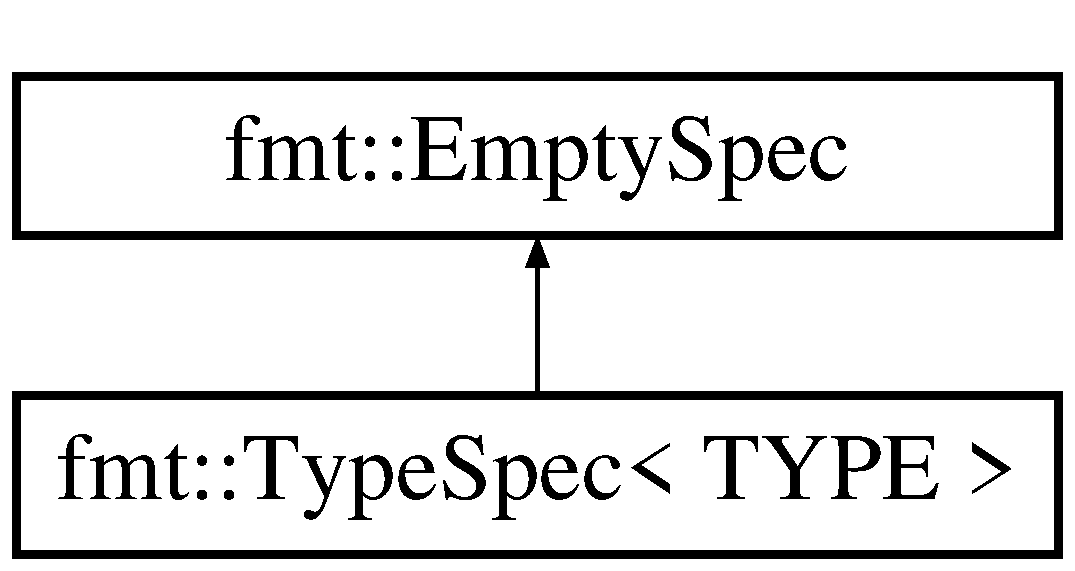
\includegraphics[height=2.000000cm]{structfmt_1_1EmptySpec}
\end{center}
\end{figure}


The documentation for this struct was generated from the following file\+:\begin{DoxyCompactItemize}
\item 
cvdi-\/src/cvdi-\/cl/include/spdlog/fmt/bundled/format.\+h\end{DoxyCompactItemize}

\hypertarget{structfmt_1_1internal_1_1EnableIf}{}\section{fmt\+:\+:internal\+:\+:Enable\+If$<$ B, T $>$ Struct Template Reference}
\label{structfmt_1_1internal_1_1EnableIf}\index{fmt\+::internal\+::\+Enable\+If$<$ B, T $>$@{fmt\+::internal\+::\+Enable\+If$<$ B, T $>$}}


The documentation for this struct was generated from the following file\+:\begin{DoxyCompactItemize}
\item 
cvdi-\/src/cvdi-\/cl/include/spdlog/fmt/bundled/format.\+h\end{DoxyCompactItemize}

\hypertarget{structfmt_1_1internal_1_1EnableIf_3_01true_00_01T_01_4}{}\section{fmt\+:\+:internal\+:\+:Enable\+If$<$ true, T $>$ Struct Template Reference}
\label{structfmt_1_1internal_1_1EnableIf_3_01true_00_01T_01_4}\index{fmt\+::internal\+::\+Enable\+If$<$ true, T $>$@{fmt\+::internal\+::\+Enable\+If$<$ true, T $>$}}
\subsection*{Public Types}
\begin{DoxyCompactItemize}
\item 
typedef T {\bfseries type}\hypertarget{structfmt_1_1internal_1_1EnableIf_3_01true_00_01T_01_4_a98d04258f45ca191b0509ef570bcc826}{}\label{structfmt_1_1internal_1_1EnableIf_3_01true_00_01T_01_4_a98d04258f45ca191b0509ef570bcc826}

\end{DoxyCompactItemize}


The documentation for this struct was generated from the following file\+:\begin{DoxyCompactItemize}
\item 
cvdi-\/src/cvdi-\/cl/include/spdlog/fmt/bundled/format.\+h\end{DoxyCompactItemize}

\hypertarget{classfmt_1_1ErrorCode}{}\section{fmt\+:\+:Error\+Code Class Reference}
\label{classfmt_1_1ErrorCode}\index{fmt\+::\+Error\+Code@{fmt\+::\+Error\+Code}}
\subsection*{Public Member Functions}
\begin{DoxyCompactItemize}
\item 
{\bfseries Error\+Code} (int value=0) F\+M\+T\+\_\+\+N\+O\+E\+X\+C\+E\+PT\hypertarget{classfmt_1_1ErrorCode_ad00ec32ba4e9a9591e856653b4d682be}{}\label{classfmt_1_1ErrorCode_ad00ec32ba4e9a9591e856653b4d682be}

\item 
int {\bfseries get} () const F\+M\+T\+\_\+\+N\+O\+E\+X\+C\+E\+PT\hypertarget{classfmt_1_1ErrorCode_a2536abb622de047cd5be707df1df7493}{}\label{classfmt_1_1ErrorCode_a2536abb622de047cd5be707df1df7493}

\end{DoxyCompactItemize}


The documentation for this class was generated from the following file\+:\begin{DoxyCompactItemize}
\item 
cvdi-\/src/cvdi-\/cl/include/spdlog/fmt/bundled/posix.\+h\end{DoxyCompactItemize}

\hypertarget{classfmt_1_1File}{}\section{fmt\+:\+:File Class Reference}
\label{classfmt_1_1File}\index{fmt\+::\+File@{fmt\+::\+File}}
\subsection*{Public Types}
\begin{DoxyCompactItemize}
\item 
enum \{ {\bfseries R\+D\+O\+N\+LY} = F\+M\+T\+\_\+\+P\+O\+S\+IX(O\+\_\+\+R\+D\+O\+N\+LY), 
{\bfseries W\+R\+O\+N\+LY} = F\+M\+T\+\_\+\+P\+O\+S\+IX(O\+\_\+\+W\+R\+O\+N\+LY), 
{\bfseries R\+D\+WR} = F\+M\+T\+\_\+\+P\+O\+S\+IX(O\+\_\+\+R\+D\+WR)
 \}\hypertarget{classfmt_1_1File_acb363a47f227d0b5821b34bb2b302dbd}{}\label{classfmt_1_1File_acb363a47f227d0b5821b34bb2b302dbd}

\end{DoxyCompactItemize}
\subsection*{Public Member Functions}
\begin{DoxyCompactItemize}
\item 
{\bfseries File} (\hyperlink{classfmt_1_1BasicCStringRef}{C\+String\+Ref} path, int oflag)\hypertarget{classfmt_1_1File_afe222b8f1728f1d803302aacba34ab0a}{}\label{classfmt_1_1File_afe222b8f1728f1d803302aacba34ab0a}

\item 
{\bfseries File} (Proxy p) F\+M\+T\+\_\+\+N\+O\+E\+X\+C\+E\+PT\hypertarget{classfmt_1_1File_af39ee41d0516e4410f935db49bc25a70}{}\label{classfmt_1_1File_af39ee41d0516e4410f935db49bc25a70}

\item 
{\bfseries File} (\hyperlink{classfmt_1_1File}{File} \&other) F\+M\+T\+\_\+\+N\+O\+E\+X\+C\+E\+PT\hypertarget{classfmt_1_1File_aa46430b90123d6ab616599c7da79baae}{}\label{classfmt_1_1File_aa46430b90123d6ab616599c7da79baae}

\item 
\hyperlink{classfmt_1_1File}{File} \& {\bfseries operator=} (Proxy p)\hypertarget{classfmt_1_1File_a49693f3a5e0cdb33e8db1e80f3bfb66d}{}\label{classfmt_1_1File_a49693f3a5e0cdb33e8db1e80f3bfb66d}

\item 
\hyperlink{classfmt_1_1File}{File} \& {\bfseries operator=} (\hyperlink{classfmt_1_1File}{File} \&other)\hypertarget{classfmt_1_1File_a0a5735314d74ec3769077e2ae1ce960a}{}\label{classfmt_1_1File_a0a5735314d74ec3769077e2ae1ce960a}

\item 
{\bfseries operator Proxy} () F\+M\+T\+\_\+\+N\+O\+E\+X\+C\+E\+PT\hypertarget{classfmt_1_1File_ab1523e72fde1f9080a4bae41dccfd824}{}\label{classfmt_1_1File_ab1523e72fde1f9080a4bae41dccfd824}

\item 
int {\bfseries descriptor} () const F\+M\+T\+\_\+\+N\+O\+E\+X\+C\+E\+PT\hypertarget{classfmt_1_1File_a19976004ecb9edfb762b5255736fe73c}{}\label{classfmt_1_1File_a19976004ecb9edfb762b5255736fe73c}

\item 
void {\bfseries close} ()\hypertarget{classfmt_1_1File_a0f9f9adfcae772efe2cae9c60a2f23f4}{}\label{classfmt_1_1File_a0f9f9adfcae772efe2cae9c60a2f23f4}

\item 
Long\+Long {\bfseries size} () const \hypertarget{classfmt_1_1File_aea68742f4f814c97d497a8a04dfc571e}{}\label{classfmt_1_1File_aea68742f4f814c97d497a8a04dfc571e}

\item 
std\+::size\+\_\+t {\bfseries read} (void $\ast$buffer, std\+::size\+\_\+t count)\hypertarget{classfmt_1_1File_abc5028be3839fafe1e54aa44bf94cb32}{}\label{classfmt_1_1File_abc5028be3839fafe1e54aa44bf94cb32}

\item 
std\+::size\+\_\+t {\bfseries write} (const void $\ast$buffer, std\+::size\+\_\+t count)\hypertarget{classfmt_1_1File_a0af6a258b5ca604680a83bada8a836d8}{}\label{classfmt_1_1File_a0af6a258b5ca604680a83bada8a836d8}

\item 
void {\bfseries dup2} (int fd)\hypertarget{classfmt_1_1File_a45718106d65eb24d0a44dbd6ef75865c}{}\label{classfmt_1_1File_a45718106d65eb24d0a44dbd6ef75865c}

\item 
void {\bfseries dup2} (int fd, \hyperlink{classfmt_1_1ErrorCode}{Error\+Code} \&ec) F\+M\+T\+\_\+\+N\+O\+E\+X\+C\+E\+PT\hypertarget{classfmt_1_1File_a2c15a1bef5be959578969a275d470011}{}\label{classfmt_1_1File_a2c15a1bef5be959578969a275d470011}

\item 
\hyperlink{classfmt_1_1BufferedFile}{Buffered\+File} {\bfseries fdopen} (const char $\ast$mode)\hypertarget{classfmt_1_1File_ab8f1cc502c78916df5f743900ea92ad4}{}\label{classfmt_1_1File_ab8f1cc502c78916df5f743900ea92ad4}

\end{DoxyCompactItemize}
\subsection*{Static Public Member Functions}
\begin{DoxyCompactItemize}
\item 
static \hyperlink{classfmt_1_1File}{File} {\bfseries dup} (int fd)\hypertarget{classfmt_1_1File_a2521de9e7f1ee48234ddc117689a3739}{}\label{classfmt_1_1File_a2521de9e7f1ee48234ddc117689a3739}

\item 
static void {\bfseries pipe} (\hyperlink{classfmt_1_1File}{File} \&read\+\_\+end, \hyperlink{classfmt_1_1File}{File} \&write\+\_\+end)\hypertarget{classfmt_1_1File_a84143751d0471636367eddbdf1269823}{}\label{classfmt_1_1File_a84143751d0471636367eddbdf1269823}

\end{DoxyCompactItemize}


The documentation for this class was generated from the following files\+:\begin{DoxyCompactItemize}
\item 
cvdi-\/src/cvdi-\/cl/include/spdlog/fmt/bundled/posix.\+h\item 
cvdi-\/src/cvdi-\/cl/include/spdlog/fmt/bundled/posix.\+cc\end{DoxyCompactItemize}

\hypertarget{classspdlog_1_1details_1_1file__helper}{}\section{spdlog\+:\+:details\+:\+:file\+\_\+helper Class Reference}
\label{classspdlog_1_1details_1_1file__helper}\index{spdlog\+::details\+::file\+\_\+helper@{spdlog\+::details\+::file\+\_\+helper}}
\subsection*{Public Member Functions}
\begin{DoxyCompactItemize}
\item 
{\bfseries file\+\_\+helper} (const \hyperlink{classspdlog_1_1details_1_1file__helper}{file\+\_\+helper} \&)=delete\hypertarget{classspdlog_1_1details_1_1file__helper_ab68b7720555f7656a8f387f8e0dcb37d}{}\label{classspdlog_1_1details_1_1file__helper_ab68b7720555f7656a8f387f8e0dcb37d}

\item 
\hyperlink{classspdlog_1_1details_1_1file__helper}{file\+\_\+helper} \& {\bfseries operator=} (const \hyperlink{classspdlog_1_1details_1_1file__helper}{file\+\_\+helper} \&)=delete\hypertarget{classspdlog_1_1details_1_1file__helper_a7c7314360e404efa02326feb7aa98442}{}\label{classspdlog_1_1details_1_1file__helper_a7c7314360e404efa02326feb7aa98442}

\item 
void {\bfseries open} (const filename\+\_\+t \&fname, bool truncate=false)\hypertarget{classspdlog_1_1details_1_1file__helper_a8612066fd098080cc60e3aefed6a6085}{}\label{classspdlog_1_1details_1_1file__helper_a8612066fd098080cc60e3aefed6a6085}

\item 
void {\bfseries reopen} (bool truncate)\hypertarget{classspdlog_1_1details_1_1file__helper_a21c688da7f241c53871b462c3a5c2c94}{}\label{classspdlog_1_1details_1_1file__helper_a21c688da7f241c53871b462c3a5c2c94}

\item 
void {\bfseries flush} ()\hypertarget{classspdlog_1_1details_1_1file__helper_a1a75f29ec0c13d9fbc269bcd8378b18b}{}\label{classspdlog_1_1details_1_1file__helper_a1a75f29ec0c13d9fbc269bcd8378b18b}

\item 
void {\bfseries close} ()\hypertarget{classspdlog_1_1details_1_1file__helper_a6a6d7a75014ae880857b4fe4fd01dc7a}{}\label{classspdlog_1_1details_1_1file__helper_a6a6d7a75014ae880857b4fe4fd01dc7a}

\item 
void {\bfseries write} (const \hyperlink{structspdlog_1_1details_1_1log__msg}{log\+\_\+msg} \&msg)\hypertarget{classspdlog_1_1details_1_1file__helper_ab86646bf59fce30003bdfedfb29768ae}{}\label{classspdlog_1_1details_1_1file__helper_ab86646bf59fce30003bdfedfb29768ae}

\item 
size\+\_\+t {\bfseries size} ()\hypertarget{classspdlog_1_1details_1_1file__helper_ad573302cd522df3ae16459625a982e12}{}\label{classspdlog_1_1details_1_1file__helper_ad573302cd522df3ae16459625a982e12}

\item 
const filename\+\_\+t \& {\bfseries filename} () const \hypertarget{classspdlog_1_1details_1_1file__helper_a3cd06d6cc27e18111ff27702d0aeee5e}{}\label{classspdlog_1_1details_1_1file__helper_a3cd06d6cc27e18111ff27702d0aeee5e}

\end{DoxyCompactItemize}
\subsection*{Static Public Member Functions}
\begin{DoxyCompactItemize}
\item 
static bool {\bfseries file\+\_\+exists} (const filename\+\_\+t \&name)\hypertarget{classspdlog_1_1details_1_1file__helper_a822cb4876d3021921acd4151e4e7e585}{}\label{classspdlog_1_1details_1_1file__helper_a822cb4876d3021921acd4151e4e7e585}

\end{DoxyCompactItemize}
\subsection*{Public Attributes}
\begin{DoxyCompactItemize}
\item 
const int {\bfseries open\+\_\+tries} = 5\hypertarget{classspdlog_1_1details_1_1file__helper_a22be952a421d866566eed3a5ce201144}{}\label{classspdlog_1_1details_1_1file__helper_a22be952a421d866566eed3a5ce201144}

\item 
const int {\bfseries open\+\_\+interval} = 10\hypertarget{classspdlog_1_1details_1_1file__helper_aea72ea8d655bb11f19dbe48477e6c8b3}{}\label{classspdlog_1_1details_1_1file__helper_aea72ea8d655bb11f19dbe48477e6c8b3}

\end{DoxyCompactItemize}


The documentation for this class was generated from the following file\+:\begin{DoxyCompactItemize}
\item 
cvdi-\/src/cvdi-\/cl/include/spdlog/details/file\+\_\+helper.\+h\end{DoxyCompactItemize}

\hypertarget{classcvdi__multi_1_1FileInfo}{}\section{cvdi\+\_\+multi\+:\+:File\+Info Class Reference}
\label{classcvdi__multi_1_1FileInfo}\index{cvdi\+\_\+multi\+::\+File\+Info@{cvdi\+\_\+multi\+::\+File\+Info}}


An abstract base class containing information about a file containing one or more trips.  




{\ttfamily \#include $<$cvdi\+\_\+multi.\+hpp$>$}

Inheritance diagram for cvdi\+\_\+multi\+:\+:File\+Info\+:\begin{figure}[H]
\begin{center}
\leavevmode
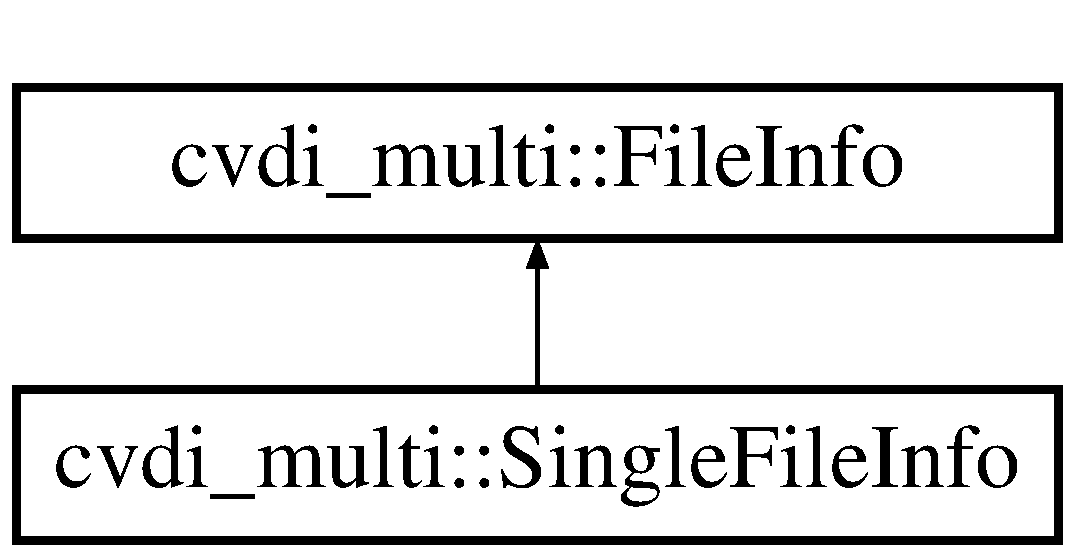
\includegraphics[height=2.000000cm]{classcvdi__multi_1_1FileInfo}
\end{center}
\end{figure}
\subsection*{Public Types}
\begin{DoxyCompactItemize}
\item 
using {\bfseries Ptr} = std\+::shared\+\_\+ptr$<$ \hyperlink{classcvdi__multi_1_1FileInfo}{File\+Info} $>$\hypertarget{classcvdi__multi_1_1FileInfo_aea599c96f681f77df5c4de62d8e7d744}{}\label{classcvdi__multi_1_1FileInfo_aea599c96f681f77df5c4de62d8e7d744}

\end{DoxyCompactItemize}
\subsection*{Public Member Functions}
\begin{DoxyCompactItemize}
\item 
virtual const std\+::string {\bfseries Get\+File\+Path} (void) const =0\hypertarget{classcvdi__multi_1_1FileInfo_ac4b8f30218d9b9d5dcb0bbfee14ad026}{}\label{classcvdi__multi_1_1FileInfo_ac4b8f30218d9b9d5dcb0bbfee14ad026}

\end{DoxyCompactItemize}


\subsection{Detailed Description}
An abstract base class containing information about a file containing one or more trips. 

The documentation for this class was generated from the following file\+:\begin{DoxyCompactItemize}
\item 
cvdi-\/src/cvdi-\/cl/include/cvdi\+\_\+multi.\+hpp\end{DoxyCompactItemize}

\hypertarget{classfmt_1_1internal_1_1FixedBuffer}{}\section{fmt\+:\+:internal\+:\+:Fixed\+Buffer$<$ Char $>$ Class Template Reference}
\label{classfmt_1_1internal_1_1FixedBuffer}\index{fmt\+::internal\+::\+Fixed\+Buffer$<$ Char $>$@{fmt\+::internal\+::\+Fixed\+Buffer$<$ Char $>$}}
Inheritance diagram for fmt\+:\+:internal\+:\+:Fixed\+Buffer$<$ Char $>$\+:\begin{figure}[H]
\begin{center}
\leavevmode
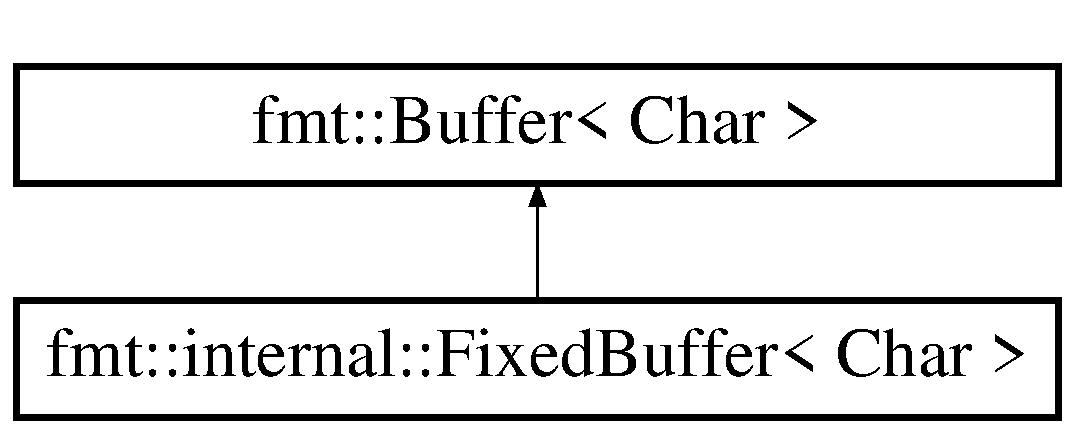
\includegraphics[height=2.000000cm]{classfmt_1_1internal_1_1FixedBuffer}
\end{center}
\end{figure}
\subsection*{Public Member Functions}
\begin{DoxyCompactItemize}
\item 
{\bfseries Fixed\+Buffer} (Char $\ast$array, std\+::size\+\_\+t \hyperlink{classfmt_1_1Buffer_a14fa72f0ddf584c14ffffb1446f598aa}{size})\hypertarget{classfmt_1_1internal_1_1FixedBuffer_a33c430838198b38592c7e9f4f6fd62d8}{}\label{classfmt_1_1internal_1_1FixedBuffer_a33c430838198b38592c7e9f4f6fd62d8}

\end{DoxyCompactItemize}
\subsection*{Protected Member Functions}
\begin{DoxyCompactItemize}
\item 
F\+M\+T\+\_\+\+A\+PI void \hyperlink{classfmt_1_1internal_1_1FixedBuffer_a90dc1dce4e8eac799d57ca519cfeb82d}{grow} (std\+::size\+\_\+t \hyperlink{classfmt_1_1Buffer_a14fa72f0ddf584c14ffffb1446f598aa}{size})
\end{DoxyCompactItemize}
\subsection*{Additional Inherited Members}


\subsection{Member Function Documentation}
\index{fmt\+::internal\+::\+Fixed\+Buffer@{fmt\+::internal\+::\+Fixed\+Buffer}!grow@{grow}}
\index{grow@{grow}!fmt\+::internal\+::\+Fixed\+Buffer@{fmt\+::internal\+::\+Fixed\+Buffer}}
\subsubsection[{\texorpdfstring{grow(std\+::size\+\_\+t size)}{grow(std::size_t size)}}]{\setlength{\rightskip}{0pt plus 5cm}template$<$typename Char $>$ template void {\bf fmt\+::internal\+::\+Fixed\+Buffer}$<$ Char $>$\+::grow (
\begin{DoxyParamCaption}
\item[{std\+::size\+\_\+t}]{size}
\end{DoxyParamCaption}
)\hspace{0.3cm}{\ttfamily [protected]}, {\ttfamily [virtual]}}\hypertarget{classfmt_1_1internal_1_1FixedBuffer_a90dc1dce4e8eac799d57ca519cfeb82d}{}\label{classfmt_1_1internal_1_1FixedBuffer_a90dc1dce4e8eac799d57ca519cfeb82d}
Increases the buffer capacity to hold at least {\itshape size} elements updating {\ttfamily ptr\+\_\+} and {\ttfamily capacity\+\_\+}.  

Implements \hyperlink{classfmt_1_1Buffer_abdc7aaf5813aa07008b3d715969a7e19}{fmt\+::\+Buffer$<$ Char $>$}.



The documentation for this class was generated from the following files\+:\begin{DoxyCompactItemize}
\item 
cvdi-\/src/cvdi-\/cl/include/spdlog/fmt/bundled/format.\+h\item 
cvdi-\/src/cvdi-\/cl/include/spdlog/fmt/bundled/format.\+cc\end{DoxyCompactItemize}

\hypertarget{classspdlog_1_1details_1_1flag__formatter}{}\section{spdlog\+:\+:details\+:\+:flag\+\_\+formatter Class Reference}
\label{classspdlog_1_1details_1_1flag__formatter}\index{spdlog\+::details\+::flag\+\_\+formatter@{spdlog\+::details\+::flag\+\_\+formatter}}
Inheritance diagram for spdlog\+:\+:details\+:\+:flag\+\_\+formatter\+:\begin{figure}[H]
\begin{center}
\leavevmode
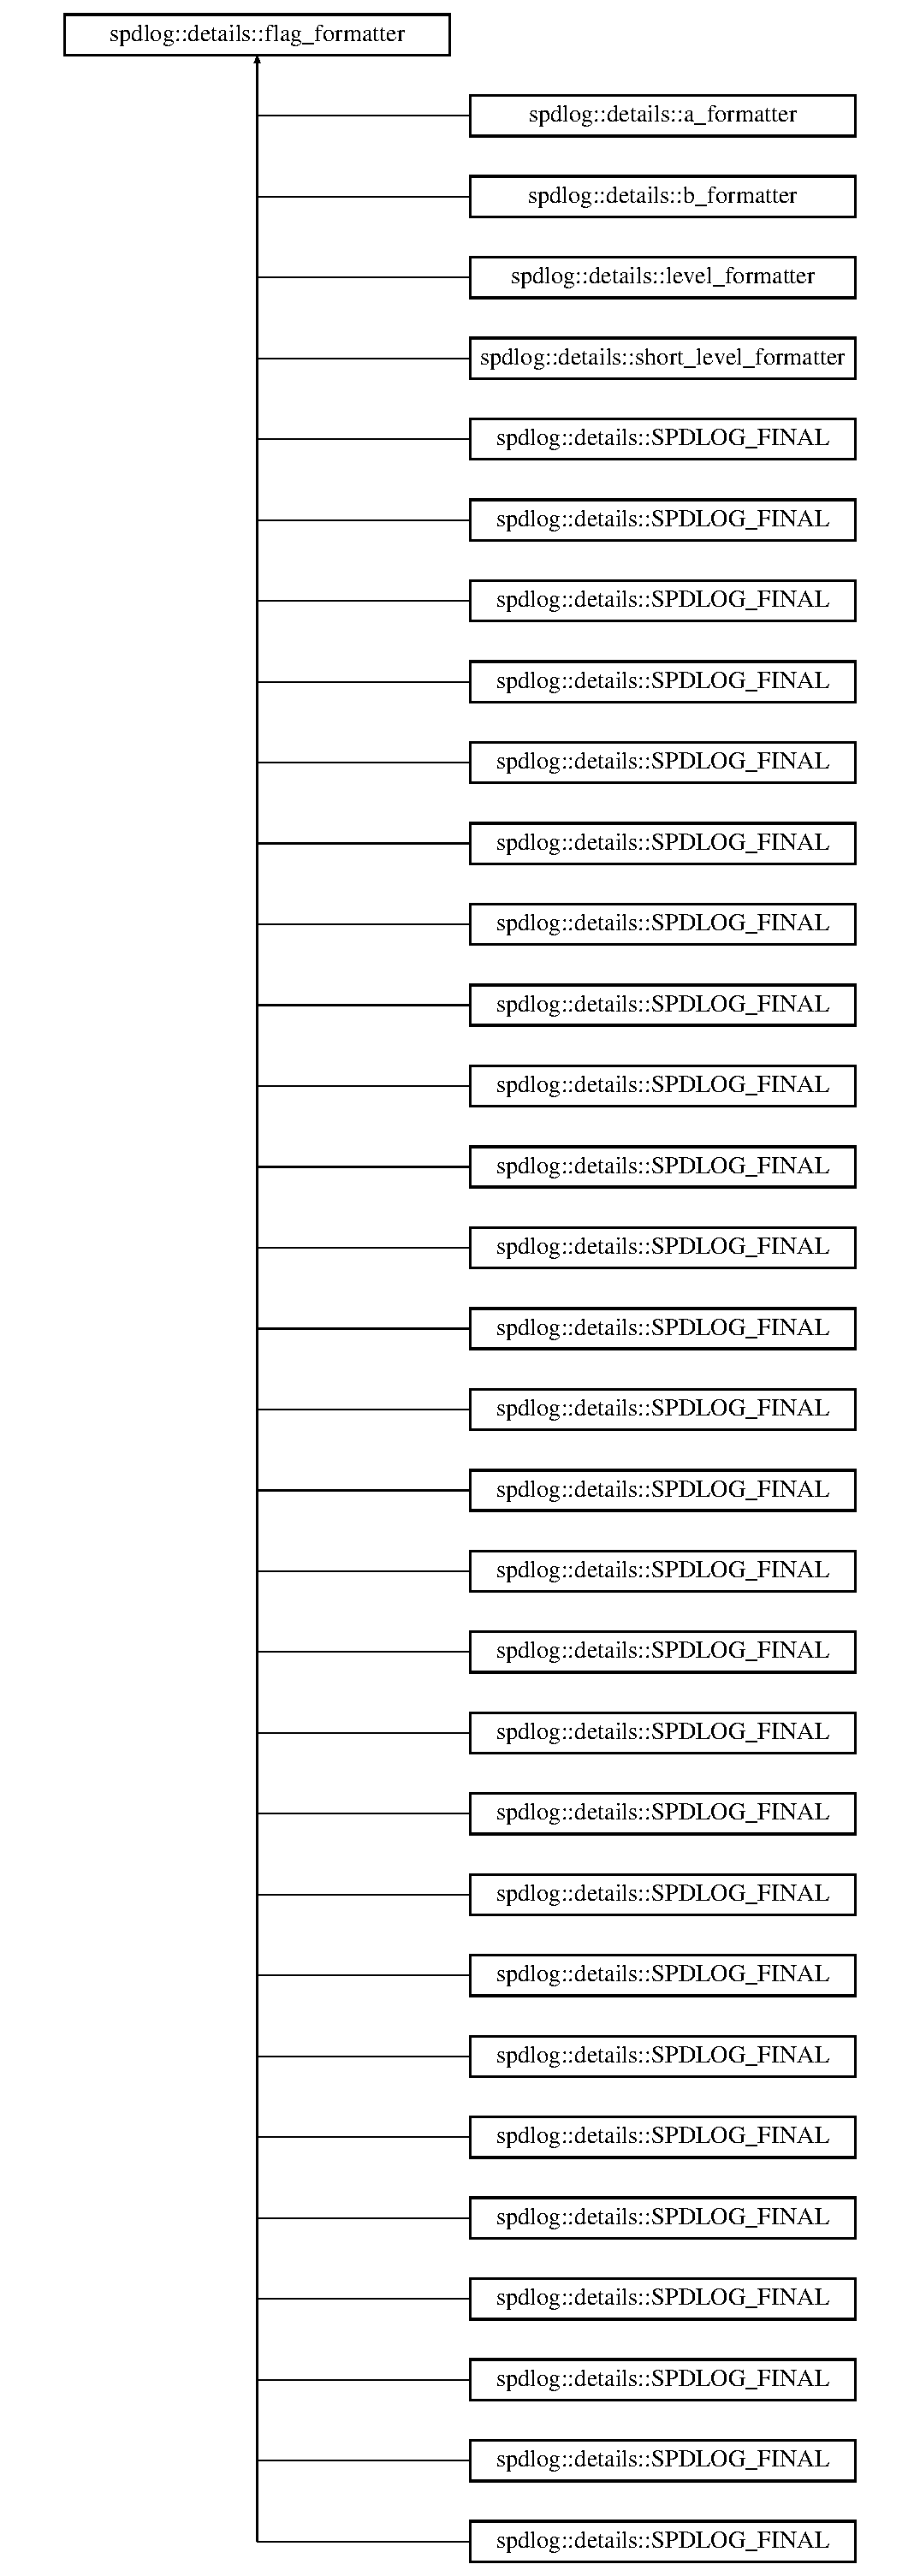
\includegraphics[height=12.000000cm]{classspdlog_1_1details_1_1flag__formatter}
\end{center}
\end{figure}
\subsection*{Public Member Functions}
\begin{DoxyCompactItemize}
\item 
virtual void {\bfseries format} (\hyperlink{structspdlog_1_1details_1_1log__msg}{details\+::log\+\_\+msg} \&msg, const std\+::tm \&tm\+\_\+time)=0\hypertarget{classspdlog_1_1details_1_1flag__formatter_a63655aca1ab3c595b80bfb79ffc37ef7}{}\label{classspdlog_1_1details_1_1flag__formatter_a63655aca1ab3c595b80bfb79ffc37ef7}

\end{DoxyCompactItemize}


The documentation for this class was generated from the following file\+:\begin{DoxyCompactItemize}
\item 
cvdi-\/src/cvdi-\/cl/include/spdlog/details/pattern\+\_\+formatter\+\_\+impl.\+h\end{DoxyCompactItemize}

\hypertarget{classfmt_1_1internal_1_1FormatBuf}{}\section{fmt\+:\+:internal\+:\+:Format\+Buf$<$ Char $>$ Class Template Reference}
\label{classfmt_1_1internal_1_1FormatBuf}\index{fmt\+::internal\+::\+Format\+Buf$<$ Char $>$@{fmt\+::internal\+::\+Format\+Buf$<$ Char $>$}}
Inheritance diagram for fmt\+:\+:internal\+:\+:Format\+Buf$<$ Char $>$\+:\begin{figure}[H]
\begin{center}
\leavevmode
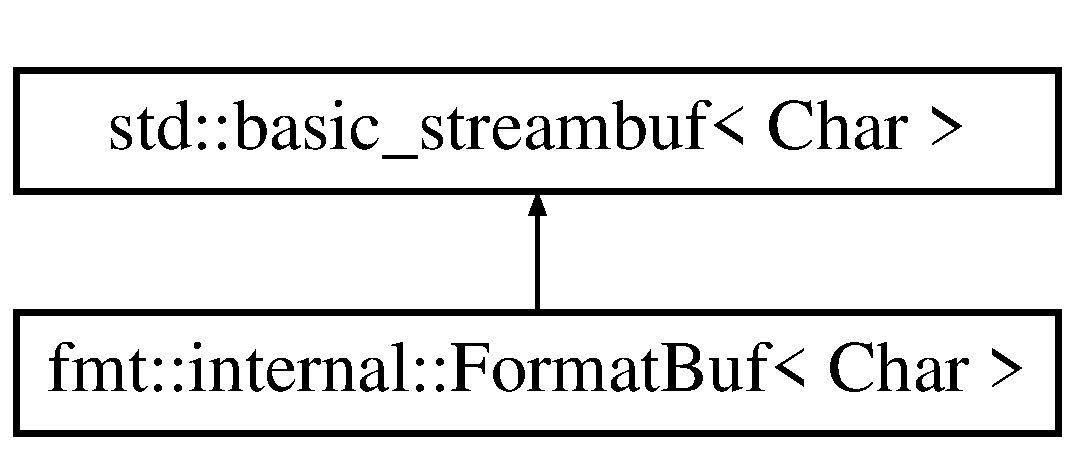
\includegraphics[height=2.000000cm]{classfmt_1_1internal_1_1FormatBuf}
\end{center}
\end{figure}
\subsection*{Public Member Functions}
\begin{DoxyCompactItemize}
\item 
{\bfseries Format\+Buf} (\hyperlink{classfmt_1_1Buffer}{Buffer}$<$ Char $>$ \&buffer)\hypertarget{classfmt_1_1internal_1_1FormatBuf_adcbde95f2bfaffd93ec7f39ae5636bfb}{}\label{classfmt_1_1internal_1_1FormatBuf_adcbde95f2bfaffd93ec7f39ae5636bfb}

\item 
int\+\_\+type {\bfseries overflow} (int\+\_\+type ch=traits\+\_\+type\+::eof())\hypertarget{classfmt_1_1internal_1_1FormatBuf_af5f472241b45d828a8d40cea7694c95c}{}\label{classfmt_1_1internal_1_1FormatBuf_af5f472241b45d828a8d40cea7694c95c}

\item 
size\+\_\+t {\bfseries size} () const \hypertarget{classfmt_1_1internal_1_1FormatBuf_a37d9219b491e9f05f22334b60cf41c5f}{}\label{classfmt_1_1internal_1_1FormatBuf_a37d9219b491e9f05f22334b60cf41c5f}

\end{DoxyCompactItemize}


The documentation for this class was generated from the following file\+:\begin{DoxyCompactItemize}
\item 
cvdi-\/src/cvdi-\/cl/include/spdlog/fmt/bundled/ostream.\+h\end{DoxyCompactItemize}

\hypertarget{classfmt_1_1FormatError}{}\section{fmt\+:\+:Format\+Error Class Reference}
\label{classfmt_1_1FormatError}\index{fmt\+::\+Format\+Error@{fmt\+::\+Format\+Error}}


{\ttfamily \#include $<$format.\+h$>$}

Inheritance diagram for fmt\+:\+:Format\+Error\+:\begin{figure}[H]
\begin{center}
\leavevmode
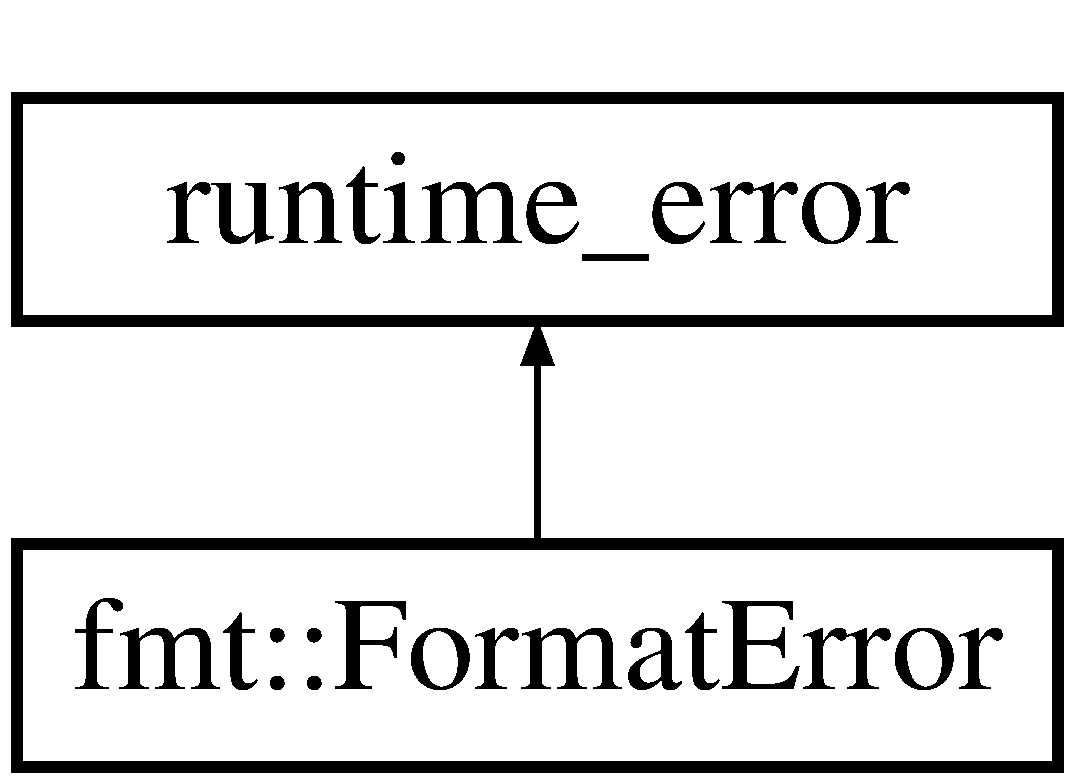
\includegraphics[height=2.000000cm]{classfmt_1_1FormatError}
\end{center}
\end{figure}
\subsection*{Public Member Functions}
\begin{DoxyCompactItemize}
\item 
{\bfseries Format\+Error} (\hyperlink{classfmt_1_1BasicCStringRef}{C\+String\+Ref} message)\hypertarget{classfmt_1_1FormatError_adceda84540093a114256a7159b30bf5e}{}\label{classfmt_1_1FormatError_adceda84540093a114256a7159b30bf5e}

\end{DoxyCompactItemize}


\subsection{Detailed Description}
A formatting error such as invalid format string. 

The documentation for this class was generated from the following files\+:\begin{DoxyCompactItemize}
\item 
cvdi-\/src/cvdi-\/cl/include/spdlog/fmt/bundled/format.\+h\item 
cvdi-\/src/cvdi-\/cl/include/spdlog/fmt/bundled/format.\+cc\end{DoxyCompactItemize}

\hypertarget{classfmt_1_1FormatInt}{}\section{fmt\+:\+:Format\+Int Class Reference}
\label{classfmt_1_1FormatInt}\index{fmt\+::\+Format\+Int@{fmt\+::\+Format\+Int}}


{\ttfamily \#include $<$format.\+h$>$}

\subsection*{Public Member Functions}
\begin{DoxyCompactItemize}
\item 
{\bfseries Format\+Int} (int value)\hypertarget{classfmt_1_1FormatInt_a9ea696341b1f8be23c41885c1bfb1395}{}\label{classfmt_1_1FormatInt_a9ea696341b1f8be23c41885c1bfb1395}

\item 
{\bfseries Format\+Int} (long value)\hypertarget{classfmt_1_1FormatInt_afba7a9464d4b9d70a877b38f09b66a30}{}\label{classfmt_1_1FormatInt_afba7a9464d4b9d70a877b38f09b66a30}

\item 
{\bfseries Format\+Int} (Long\+Long value)\hypertarget{classfmt_1_1FormatInt_af1e95a3f28e4905ed901beb1df3d77e2}{}\label{classfmt_1_1FormatInt_af1e95a3f28e4905ed901beb1df3d77e2}

\item 
{\bfseries Format\+Int} (unsigned value)\hypertarget{classfmt_1_1FormatInt_a6bbe09f7223c6489272ae295330c145c}{}\label{classfmt_1_1FormatInt_a6bbe09f7223c6489272ae295330c145c}

\item 
{\bfseries Format\+Int} (unsigned long value)\hypertarget{classfmt_1_1FormatInt_a376433048225d105887f0a151126c134}{}\label{classfmt_1_1FormatInt_a376433048225d105887f0a151126c134}

\item 
{\bfseries Format\+Int} (U\+Long\+Long value)\hypertarget{classfmt_1_1FormatInt_ace4887e009064bcea8eea9bb6e30026e}{}\label{classfmt_1_1FormatInt_ace4887e009064bcea8eea9bb6e30026e}

\item 
std\+::size\+\_\+t \hyperlink{classfmt_1_1FormatInt_ad09445e55ae7c8944b5275a54a03da14}{size} () const 
\item 
const char $\ast$ \hyperlink{classfmt_1_1FormatInt_a3cad581dde135c51390fd4ebd18d6d1b}{data} () const 
\item 
const char $\ast$ \hyperlink{classfmt_1_1FormatInt_a58a17394f4f8e63debb91b90aa0dea0c}{c\+\_\+str} () const 
\item 
std\+::string \hyperlink{classfmt_1_1FormatInt_adfd4854a5efceb8df461a521c3eda5ef}{str} () const 
\end{DoxyCompactItemize}


\subsection{Detailed Description}
Fast integer formatter. 

\subsection{Member Function Documentation}
\index{fmt\+::\+Format\+Int@{fmt\+::\+Format\+Int}!c\+\_\+str@{c\+\_\+str}}
\index{c\+\_\+str@{c\+\_\+str}!fmt\+::\+Format\+Int@{fmt\+::\+Format\+Int}}
\subsubsection[{\texorpdfstring{c\+\_\+str() const }{c_str() const }}]{\setlength{\rightskip}{0pt plus 5cm}const char$\ast$ fmt\+::\+Format\+Int\+::c\+\_\+str (
\begin{DoxyParamCaption}
{}
\end{DoxyParamCaption}
) const\hspace{0.3cm}{\ttfamily [inline]}}\hypertarget{classfmt_1_1FormatInt_a58a17394f4f8e63debb91b90aa0dea0c}{}\label{classfmt_1_1FormatInt_a58a17394f4f8e63debb91b90aa0dea0c}
Returns a pointer to the output buffer content with terminating null character appended. \index{fmt\+::\+Format\+Int@{fmt\+::\+Format\+Int}!data@{data}}
\index{data@{data}!fmt\+::\+Format\+Int@{fmt\+::\+Format\+Int}}
\subsubsection[{\texorpdfstring{data() const }{data() const }}]{\setlength{\rightskip}{0pt plus 5cm}const char$\ast$ fmt\+::\+Format\+Int\+::data (
\begin{DoxyParamCaption}
{}
\end{DoxyParamCaption}
) const\hspace{0.3cm}{\ttfamily [inline]}}\hypertarget{classfmt_1_1FormatInt_a3cad581dde135c51390fd4ebd18d6d1b}{}\label{classfmt_1_1FormatInt_a3cad581dde135c51390fd4ebd18d6d1b}
Returns a pointer to the output buffer content. No terminating null character is appended. \index{fmt\+::\+Format\+Int@{fmt\+::\+Format\+Int}!size@{size}}
\index{size@{size}!fmt\+::\+Format\+Int@{fmt\+::\+Format\+Int}}
\subsubsection[{\texorpdfstring{size() const }{size() const }}]{\setlength{\rightskip}{0pt plus 5cm}std\+::size\+\_\+t fmt\+::\+Format\+Int\+::size (
\begin{DoxyParamCaption}
{}
\end{DoxyParamCaption}
) const\hspace{0.3cm}{\ttfamily [inline]}}\hypertarget{classfmt_1_1FormatInt_ad09445e55ae7c8944b5275a54a03da14}{}\label{classfmt_1_1FormatInt_ad09445e55ae7c8944b5275a54a03da14}
Returns the number of characters written to the output buffer. \index{fmt\+::\+Format\+Int@{fmt\+::\+Format\+Int}!str@{str}}
\index{str@{str}!fmt\+::\+Format\+Int@{fmt\+::\+Format\+Int}}
\subsubsection[{\texorpdfstring{str() const }{str() const }}]{\setlength{\rightskip}{0pt plus 5cm}std\+::string fmt\+::\+Format\+Int\+::str (
\begin{DoxyParamCaption}
{}
\end{DoxyParamCaption}
) const\hspace{0.3cm}{\ttfamily [inline]}}\hypertarget{classfmt_1_1FormatInt_adfd4854a5efceb8df461a521c3eda5ef}{}\label{classfmt_1_1FormatInt_adfd4854a5efceb8df461a521c3eda5ef}
Returns the content of the output buffer as an {\ttfamily std\+::string}.  

The documentation for this class was generated from the following file\+:\begin{DoxyCompactItemize}
\item 
cvdi-\/src/cvdi-\/cl/include/spdlog/fmt/bundled/format.\+h\end{DoxyCompactItemize}

\hypertarget{structfmt_1_1FormatSpec}{}\section{fmt\+:\+:Format\+Spec Struct Reference}
\label{structfmt_1_1FormatSpec}\index{fmt\+::\+Format\+Spec@{fmt\+::\+Format\+Spec}}
Inheritance diagram for fmt\+:\+:Format\+Spec\+:\begin{figure}[H]
\begin{center}
\leavevmode
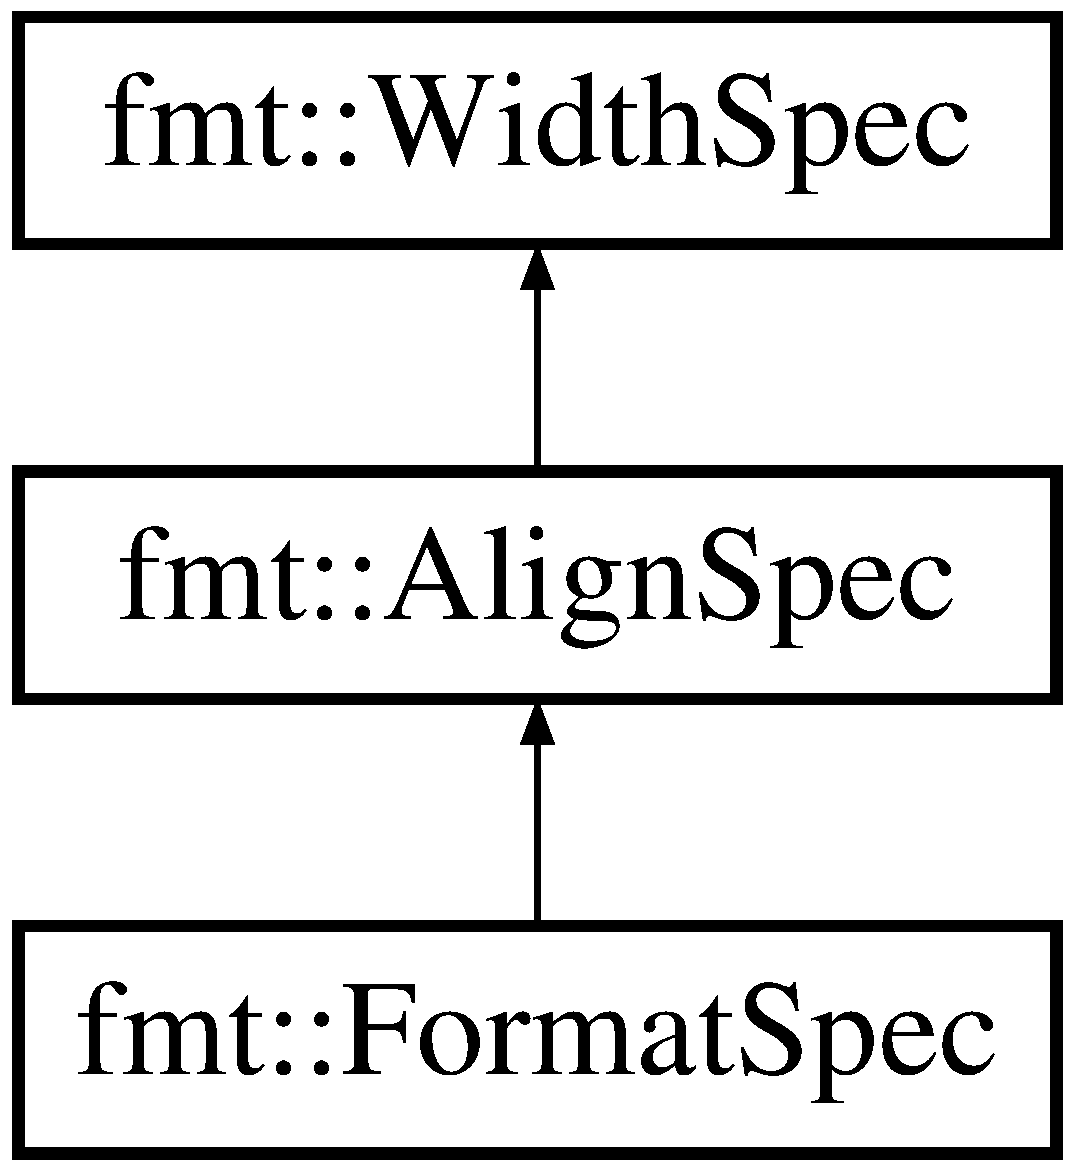
\includegraphics[height=3.000000cm]{structfmt_1_1FormatSpec}
\end{center}
\end{figure}
\subsection*{Public Member Functions}
\begin{DoxyCompactItemize}
\item 
{\bfseries Format\+Spec} (unsigned width=0, char type=0, wchar\+\_\+t fill= \textquotesingle{} \textquotesingle{})\hypertarget{structfmt_1_1FormatSpec_a6a434aa4ea0d694e10b079b4e52ffe97}{}\label{structfmt_1_1FormatSpec_a6a434aa4ea0d694e10b079b4e52ffe97}

\item 
bool {\bfseries flag} (unsigned f) const \hypertarget{structfmt_1_1FormatSpec_a2ee0e9bf9979641418a8b30b4e7740f2}{}\label{structfmt_1_1FormatSpec_a2ee0e9bf9979641418a8b30b4e7740f2}

\item 
int {\bfseries precision} () const \hypertarget{structfmt_1_1FormatSpec_a4d48f0000dc495b3cc1c6f222e2036a9}{}\label{structfmt_1_1FormatSpec_a4d48f0000dc495b3cc1c6f222e2036a9}

\item 
char {\bfseries type} () const \hypertarget{structfmt_1_1FormatSpec_a4da20f7a988a694ce02f01d1ffb3d783}{}\label{structfmt_1_1FormatSpec_a4da20f7a988a694ce02f01d1ffb3d783}

\end{DoxyCompactItemize}
\subsection*{Public Attributes}
\begin{DoxyCompactItemize}
\item 
unsigned {\bfseries flags\+\_\+}\hypertarget{structfmt_1_1FormatSpec_a9fbd00ed2b8e3b96eaa2beb54aff641e}{}\label{structfmt_1_1FormatSpec_a9fbd00ed2b8e3b96eaa2beb54aff641e}

\item 
int {\bfseries precision\+\_\+}\hypertarget{structfmt_1_1FormatSpec_a8444724bdd0a55bf3226a17e321c12c5}{}\label{structfmt_1_1FormatSpec_a8444724bdd0a55bf3226a17e321c12c5}

\item 
char {\bfseries type\+\_\+}\hypertarget{structfmt_1_1FormatSpec_aa6f085ef583f708dde9636c03adea6ab}{}\label{structfmt_1_1FormatSpec_aa6f085ef583f708dde9636c03adea6ab}

\end{DoxyCompactItemize}


The documentation for this struct was generated from the following file\+:\begin{DoxyCompactItemize}
\item 
cvdi-\/src/cvdi-\/cl/include/spdlog/fmt/bundled/format.\+h\end{DoxyCompactItemize}

\hypertarget{classspdlog_1_1formatter}{}\section{spdlog\+:\+:formatter Class Reference}
\label{classspdlog_1_1formatter}\index{spdlog\+::formatter@{spdlog\+::formatter}}
Inheritance diagram for spdlog\+:\+:formatter\+:\begin{figure}[H]
\begin{center}
\leavevmode
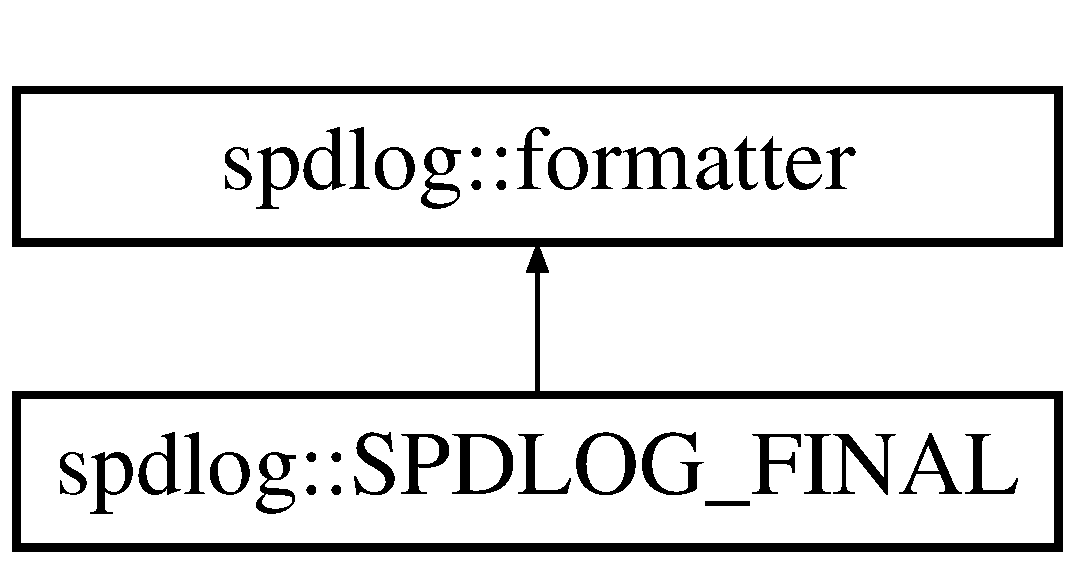
\includegraphics[height=2.000000cm]{classspdlog_1_1formatter}
\end{center}
\end{figure}
\subsection*{Public Member Functions}
\begin{DoxyCompactItemize}
\item 
virtual void {\bfseries format} (\hyperlink{structspdlog_1_1details_1_1log__msg}{details\+::log\+\_\+msg} \&msg)=0\hypertarget{classspdlog_1_1formatter_a514e1e22aba06bfd8f2bfb9c5789a858}{}\label{classspdlog_1_1formatter_a514e1e22aba06bfd8f2bfb9c5789a858}

\end{DoxyCompactItemize}


The documentation for this class was generated from the following file\+:\begin{DoxyCompactItemize}
\item 
cvdi-\/src/cvdi-\/cl/include/spdlog/formatter.\+h\end{DoxyCompactItemize}

\hypertarget{classfmt_1_1internal_1_1FormatterBase}{}\section{fmt\+:\+:internal\+:\+:Formatter\+Base Class Reference}
\label{classfmt_1_1internal_1_1FormatterBase}\index{fmt\+::internal\+::\+Formatter\+Base@{fmt\+::internal\+::\+Formatter\+Base}}
Inheritance diagram for fmt\+:\+:internal\+:\+:Formatter\+Base\+:\begin{figure}[H]
\begin{center}
\leavevmode
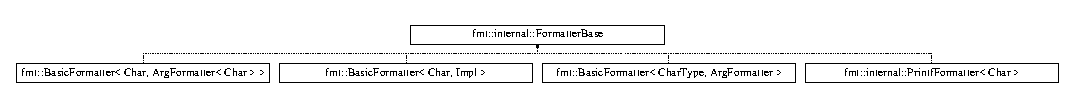
\includegraphics[height=0.888889cm]{classfmt_1_1internal_1_1FormatterBase}
\end{center}
\end{figure}
\subsection*{Protected Member Functions}
\begin{DoxyCompactItemize}
\item 
const \hyperlink{classfmt_1_1ArgList}{Arg\+List} \& {\bfseries args} () const \hypertarget{classfmt_1_1internal_1_1FormatterBase_a6b7a3a49a08e76e915400748f3cbe7fc}{}\label{classfmt_1_1internal_1_1FormatterBase_a6b7a3a49a08e76e915400748f3cbe7fc}

\item 
{\bfseries Formatter\+Base} (const \hyperlink{classfmt_1_1ArgList}{Arg\+List} \&args)\hypertarget{classfmt_1_1internal_1_1FormatterBase_a5a27cf6bbba1b7e159bb21e12453c216}{}\label{classfmt_1_1internal_1_1FormatterBase_a5a27cf6bbba1b7e159bb21e12453c216}

\item 
\hyperlink{structfmt_1_1internal_1_1Arg}{Arg} {\bfseries next\+\_\+arg} (const char $\ast$\&error)\hypertarget{classfmt_1_1internal_1_1FormatterBase_ac3d5811aa9b695596fe0dc67f870e3d4}{}\label{classfmt_1_1internal_1_1FormatterBase_ac3d5811aa9b695596fe0dc67f870e3d4}

\item 
\hyperlink{structfmt_1_1internal_1_1Arg}{Arg} {\bfseries get\+\_\+arg} (unsigned arg\+\_\+index, const char $\ast$\&error)\hypertarget{classfmt_1_1internal_1_1FormatterBase_ad5baca90f220f3f54c0c4a620ec80b7b}{}\label{classfmt_1_1internal_1_1FormatterBase_ad5baca90f220f3f54c0c4a620ec80b7b}

\item 
bool {\bfseries check\+\_\+no\+\_\+auto\+\_\+index} (const char $\ast$\&error)\hypertarget{classfmt_1_1internal_1_1FormatterBase_a27444362817694c52d86723bd2b62390}{}\label{classfmt_1_1internal_1_1FormatterBase_a27444362817694c52d86723bd2b62390}

\item 
{\footnotesize template$<$typename Char $>$ }\\void {\bfseries write} (\hyperlink{classfmt_1_1BasicWriter}{Basic\+Writer}$<$ Char $>$ \&w, const Char $\ast$start, const Char $\ast$end)\hypertarget{classfmt_1_1internal_1_1FormatterBase_ab29b5470b0f02edfde9b81ba24a51bf6}{}\label{classfmt_1_1internal_1_1FormatterBase_ab29b5470b0f02edfde9b81ba24a51bf6}

\end{DoxyCompactItemize}


The documentation for this class was generated from the following files\+:\begin{DoxyCompactItemize}
\item 
cvdi-\/src/cvdi-\/cl/include/spdlog/fmt/bundled/format.\+h\item 
cvdi-\/src/cvdi-\/cl/include/spdlog/fmt/bundled/format.\+cc\end{DoxyCompactItemize}

\hypertarget{classcvdi_1_1IntersectionCounter}{}\section{cvdi\+:\+:Intersection\+Counter Class Reference}
\label{classcvdi_1_1IntersectionCounter}\index{cvdi\+::\+Intersection\+Counter@{cvdi\+::\+Intersection\+Counter}}


Annotate a trace with a cumulative count of intersection out degree.  




{\ttfamily \#include $<$cvdi.\+hpp$>$}

\subsection*{Public Member Functions}
\begin{DoxyCompactItemize}
\item 
\hyperlink{classcvdi_1_1IntersectionCounter_ac6e71f51b6686f8f39fd19f2cd85fb5f}{Intersection\+Counter} ()\hypertarget{classcvdi_1_1IntersectionCounter_ac6e71f51b6686f8f39fd19f2cd85fb5f}{}\label{classcvdi_1_1IntersectionCounter_ac6e71f51b6686f8f39fd19f2cd85fb5f}

\begin{DoxyCompactList}\small\item\em Construct an \hyperlink{classcvdi_1_1IntersectionCounter}{Intersection\+Counter} object. \end{DoxyCompactList}\item 
void \hyperlink{classcvdi_1_1IntersectionCounter_a9be51eac7462fc03c5c6bb5cca5894dc}{count\+\_\+intersections} (geo\+\_\+data\+::\+Sample\+::\+Trace \&trace)
\begin{DoxyCompactList}\small\item\em Annotate trace with its cumulative intersection out degree counts. \end{DoxyCompactList}\end{DoxyCompactItemize}


\subsection{Detailed Description}
Annotate a trace with a cumulative count of intersection out degree. 

\subsection{Member Function Documentation}
\index{cvdi\+::\+Intersection\+Counter@{cvdi\+::\+Intersection\+Counter}!count\+\_\+intersections@{count\+\_\+intersections}}
\index{count\+\_\+intersections@{count\+\_\+intersections}!cvdi\+::\+Intersection\+Counter@{cvdi\+::\+Intersection\+Counter}}
\subsubsection[{\texorpdfstring{count\+\_\+intersections(geo\+\_\+data\+::\+Sample\+::\+Trace \&trace)}{count_intersections(geo_data::Sample::Trace &trace)}}]{\setlength{\rightskip}{0pt plus 5cm}void cvdi\+::\+Intersection\+Counter\+::count\+\_\+intersections (
\begin{DoxyParamCaption}
\item[{geo\+\_\+data\+::\+Sample\+::\+Trace \&}]{trace}
\end{DoxyParamCaption}
)}\hypertarget{classcvdi_1_1IntersectionCounter_a9be51eac7462fc03c5c6bb5cca5894dc}{}\label{classcvdi_1_1IntersectionCounter_a9be51eac7462fc03c5c6bb5cca5894dc}


Annotate trace with its cumulative intersection out degree counts. 


\begin{DoxyParams}{Parameters}
{\em trace} & the trace to annotate \\
\hline
\end{DoxyParams}


The documentation for this class was generated from the following files\+:\begin{DoxyCompactItemize}
\item 
cvdi-\/src/cvdi/include/cvdi.\+hpp\item 
cvdi-\/src/cvdi/src/cvdi.\+cpp\end{DoxyCompactItemize}

\hypertarget{classgeo__data_1_1Interval}{}\section{geo\+\_\+data\+:\+:Interval Class Reference}
\label{classgeo__data_1_1Interval}\index{geo\+\_\+data\+::\+Interval@{geo\+\_\+data\+::\+Interval}}


An integer-\/based interval class to be used with trajectories.  




{\ttfamily \#include $<$geo\+\_\+data.\+hpp$>$}

\subsection*{Public Types}
\begin{DoxyCompactItemize}
\item 
using {\bfseries Ptr} = std\+::shared\+\_\+ptr$<$ \hyperlink{classgeo__data_1_1Interval}{Interval} $>$\hypertarget{classgeo__data_1_1Interval_a36abd263b41898cd7253324766eb8445}{}\label{classgeo__data_1_1Interval_a36abd263b41898cd7253324766eb8445}

\item 
using {\bfseries Ptr\+List} = std\+::vector$<$ Ptr $>$\hypertarget{classgeo__data_1_1Interval_a8379b2779f3f02d47379e8b5dc693dd0}{}\label{classgeo__data_1_1Interval_a8379b2779f3f02d47379e8b5dc693dd0}

\item 
using {\bfseries Aux\+Set} = std\+::unordered\+\_\+set$<$ std\+::string $>$\hypertarget{classgeo__data_1_1Interval_aab3ed186003e96d4dee524d9aa34af62}{}\label{classgeo__data_1_1Interval_aab3ed186003e96d4dee524d9aa34af62}

\item 
using {\bfseries Aux\+Set\+Ptr} = std\+::shared\+\_\+ptr$<$ Aux\+Set $>$\hypertarget{classgeo__data_1_1Interval_a123802b451cf0337042034f32e3f3364}{}\label{classgeo__data_1_1Interval_a123802b451cf0337042034f32e3f3364}

\end{DoxyCompactItemize}
\subsection*{Public Member Functions}
\begin{DoxyCompactItemize}
\item 
\hyperlink{classgeo__data_1_1Interval_a4aeb907d55df262185dfe06dfb204aa5}{Interval} (Index \hyperlink{classgeo__data_1_1Interval_aa6803997160a6d97fe84c63440642a10}{left}, Index \hyperlink{classgeo__data_1_1Interval_af952a082fcbaba214c19b8e647e9f04e}{right}, std\+::string aux=\char`\"{}\char`\"{}, uint32\+\_\+t \hyperlink{classgeo__data_1_1Interval_a5a20c0a449ed531de53fe529dec35308}{type}=0)
\begin{DoxyCompactList}\small\item\em Construct the interval \mbox{[}left,right\mbox{]}. \end{DoxyCompactList}\item 
\hyperlink{classgeo__data_1_1Interval_ab5246430a8062908f45206ee48e05ec6}{Interval} (Index \hyperlink{classgeo__data_1_1Interval_aa6803997160a6d97fe84c63440642a10}{left}, Index \hyperlink{classgeo__data_1_1Interval_af952a082fcbaba214c19b8e647e9f04e}{right}, Aux\+Set\+Ptr aux\+\_\+set\+\_\+ptr, uint32\+\_\+t \hyperlink{classgeo__data_1_1Interval_a5a20c0a449ed531de53fe529dec35308}{type}=0)
\begin{DoxyCompactList}\small\item\em Construct the interval \mbox{[}left,right\mbox{]}. \end{DoxyCompactList}\item 
uint32\+\_\+t \hyperlink{classgeo__data_1_1Interval_a5a20c0a449ed531de53fe529dec35308}{type} () const 
\begin{DoxyCompactList}\small\item\em Get the interval type. \end{DoxyCompactList}\item 
Index \hyperlink{classgeo__data_1_1Interval_af952a082fcbaba214c19b8e647e9f04e}{right} () const 
\begin{DoxyCompactList}\small\item\em Get the upper bound of the interval. \end{DoxyCompactList}\item 
Index \hyperlink{classgeo__data_1_1Interval_aa6803997160a6d97fe84c63440642a10}{left} () const 
\begin{DoxyCompactList}\small\item\em Get the lower bound of the interval. \end{DoxyCompactList}\item 
Aux\+Set\+Ptr \hyperlink{classgeo__data_1_1Interval_a929e1e46a0c0ad5ab22627ce6166f09a}{aux\+\_\+set} () const 
\begin{DoxyCompactList}\small\item\em Get the auxiliary data set as a pointer. \end{DoxyCompactList}\item 
const std\+::string \hyperlink{classgeo__data_1_1Interval_a2e87ef8f764694e616244a6e9fd1d2a1}{aux\+\_\+str} (void) const 
\begin{DoxyCompactList}\small\item\em Get the auxiliary data set as a single semicolon delimited string. \end{DoxyCompactList}\item 
bool \hyperlink{classgeo__data_1_1Interval_a30406828bf5a2cc80a345b0a6a7356c6}{is\+\_\+before} (Index value) const 
\begin{DoxyCompactList}\small\item\em Predicate\+: interval upper bound $<$= value. \end{DoxyCompactList}\item 
bool \hyperlink{classgeo__data_1_1Interval_a64cd0e0eb27d67f9cfaf3d5355416892}{contains} (Index value) const 
\begin{DoxyCompactList}\small\item\em Predicate\+: value in \mbox{[}lower bound, upper bound); this check uses a right open interval. \end{DoxyCompactList}\end{DoxyCompactItemize}
\subsection*{Friends}
\begin{DoxyCompactItemize}
\item 
std\+::ostream \& \hyperlink{classgeo__data_1_1Interval_ac95b512584f3f7b577829ab5f2331c0f}{operator$<$$<$} (std\+::ostream \&os, const \hyperlink{classgeo__data_1_1Interval}{Interval} \&interval)
\begin{DoxyCompactList}\small\item\em Write the string form (id = x \mbox{[}lower bound, upper bound) types\+: \{ $<$aux data$>$=\char`\"{}\char`\"{}$>$ \}) of an \hyperlink{classgeo__data_1_1Interval}{Interval} to an output stream. \end{DoxyCompactList}\end{DoxyCompactItemize}


\subsection{Detailed Description}
An integer-\/based interval class to be used with trajectories. 

\subsection{Constructor \& Destructor Documentation}
\index{geo\+\_\+data\+::\+Interval@{geo\+\_\+data\+::\+Interval}!Interval@{Interval}}
\index{Interval@{Interval}!geo\+\_\+data\+::\+Interval@{geo\+\_\+data\+::\+Interval}}
\subsubsection[{\texorpdfstring{Interval(\+Index left, Index right, std\+::string aux="""", uint32\+\_\+t type=0)}{Interval(Index left, Index right, std::string aux="", uint32_t type=0)}}]{\setlength{\rightskip}{0pt plus 5cm}geo\+\_\+data\+::\+Interval\+::\+Interval (
\begin{DoxyParamCaption}
\item[{Index}]{left, }
\item[{Index}]{right, }
\item[{std\+::string}]{aux = {\ttfamily \char`\"{}\char`\"{}}, }
\item[{uint32\+\_\+t}]{type = {\ttfamily 0}}
\end{DoxyParamCaption}
)}\hypertarget{classgeo__data_1_1Interval_a4aeb907d55df262185dfe06dfb204aa5}{}\label{classgeo__data_1_1Interval_a4aeb907d55df262185dfe06dfb204aa5}


Construct the interval \mbox{[}left,right\mbox{]}. 


\begin{DoxyParams}{Parameters}
{\em left} & the lower bound of the interval \\
\hline
{\em right} & the upper bound of the interval \\
\hline
{\em aux} & a description of the interval \\
\hline
{\em id} & a type identifier for the interval \\
\hline
\end{DoxyParams}
\index{geo\+\_\+data\+::\+Interval@{geo\+\_\+data\+::\+Interval}!Interval@{Interval}}
\index{Interval@{Interval}!geo\+\_\+data\+::\+Interval@{geo\+\_\+data\+::\+Interval}}
\subsubsection[{\texorpdfstring{Interval(\+Index left, Index right, Aux\+Set\+Ptr aux\+\_\+set\+\_\+ptr, uint32\+\_\+t type=0)}{Interval(Index left, Index right, AuxSetPtr aux_set_ptr, uint32_t type=0)}}]{\setlength{\rightskip}{0pt plus 5cm}geo\+\_\+data\+::\+Interval\+::\+Interval (
\begin{DoxyParamCaption}
\item[{Index}]{left, }
\item[{Index}]{right, }
\item[{Interval\+::\+Aux\+Set\+Ptr}]{aux\+\_\+set, }
\item[{uint32\+\_\+t}]{type = {\ttfamily 0}}
\end{DoxyParamCaption}
)}\hypertarget{classgeo__data_1_1Interval_ab5246430a8062908f45206ee48e05ec6}{}\label{classgeo__data_1_1Interval_ab5246430a8062908f45206ee48e05ec6}


Construct the interval \mbox{[}left,right\mbox{]}. 


\begin{DoxyParams}{Parameters}
{\em left} & the infimum of the interval \\
\hline
{\em right} & the supremum of the interval \\
\hline
{\em aux} & a description of the interval \\
\hline
{\em id} & a type identifier for the interval \\
\hline
\end{DoxyParams}


\subsection{Member Function Documentation}
\index{geo\+\_\+data\+::\+Interval@{geo\+\_\+data\+::\+Interval}!aux\+\_\+set@{aux\+\_\+set}}
\index{aux\+\_\+set@{aux\+\_\+set}!geo\+\_\+data\+::\+Interval@{geo\+\_\+data\+::\+Interval}}
\subsubsection[{\texorpdfstring{aux\+\_\+set() const }{aux_set() const }}]{\setlength{\rightskip}{0pt plus 5cm}Interval\+::\+Aux\+Set\+Ptr geo\+\_\+data\+::\+Interval\+::aux\+\_\+set (
\begin{DoxyParamCaption}
{}
\end{DoxyParamCaption}
) const}\hypertarget{classgeo__data_1_1Interval_a929e1e46a0c0ad5ab22627ce6166f09a}{}\label{classgeo__data_1_1Interval_a929e1e46a0c0ad5ab22627ce6166f09a}


Get the auxiliary data set as a pointer. 

\begin{DoxyReturn}{Returns}
the set of strings that represent the auxiliary data 
\end{DoxyReturn}
\index{geo\+\_\+data\+::\+Interval@{geo\+\_\+data\+::\+Interval}!aux\+\_\+str@{aux\+\_\+str}}
\index{aux\+\_\+str@{aux\+\_\+str}!geo\+\_\+data\+::\+Interval@{geo\+\_\+data\+::\+Interval}}
\subsubsection[{\texorpdfstring{aux\+\_\+str(void) const }{aux_str(void) const }}]{\setlength{\rightskip}{0pt plus 5cm}const std\+::string geo\+\_\+data\+::\+Interval\+::aux\+\_\+str (
\begin{DoxyParamCaption}
\item[{void}]{}
\end{DoxyParamCaption}
) const}\hypertarget{classgeo__data_1_1Interval_a2e87ef8f764694e616244a6e9fd1d2a1}{}\label{classgeo__data_1_1Interval_a2e87ef8f764694e616244a6e9fd1d2a1}


Get the auxiliary data set as a single semicolon delimited string. 

\begin{DoxyReturn}{Returns}
the auxiliary data set as one string 
\end{DoxyReturn}
\index{geo\+\_\+data\+::\+Interval@{geo\+\_\+data\+::\+Interval}!contains@{contains}}
\index{contains@{contains}!geo\+\_\+data\+::\+Interval@{geo\+\_\+data\+::\+Interval}}
\subsubsection[{\texorpdfstring{contains(\+Index value) const }{contains(Index value) const }}]{\setlength{\rightskip}{0pt plus 5cm}bool geo\+\_\+data\+::\+Interval\+::contains (
\begin{DoxyParamCaption}
\item[{Index}]{value}
\end{DoxyParamCaption}
) const}\hypertarget{classgeo__data_1_1Interval_a64cd0e0eb27d67f9cfaf3d5355416892}{}\label{classgeo__data_1_1Interval_a64cd0e0eb27d67f9cfaf3d5355416892}


Predicate\+: value in \mbox{[}lower bound, upper bound); this check uses a right open interval. 

\begin{DoxyReturn}{Returns}
true if lower bound $<$= value $<$ upper bound, false otherwise 
\end{DoxyReturn}
\index{geo\+\_\+data\+::\+Interval@{geo\+\_\+data\+::\+Interval}!is\+\_\+before@{is\+\_\+before}}
\index{is\+\_\+before@{is\+\_\+before}!geo\+\_\+data\+::\+Interval@{geo\+\_\+data\+::\+Interval}}
\subsubsection[{\texorpdfstring{is\+\_\+before(\+Index value) const }{is_before(Index value) const }}]{\setlength{\rightskip}{0pt plus 5cm}bool geo\+\_\+data\+::\+Interval\+::is\+\_\+before (
\begin{DoxyParamCaption}
\item[{Index}]{value}
\end{DoxyParamCaption}
) const}\hypertarget{classgeo__data_1_1Interval_a30406828bf5a2cc80a345b0a6a7356c6}{}\label{classgeo__data_1_1Interval_a30406828bf5a2cc80a345b0a6a7356c6}


Predicate\+: interval upper bound $<$= value. 

\begin{DoxyReturn}{Returns}
true if interval upper bound $<$= value 
\end{DoxyReturn}
\index{geo\+\_\+data\+::\+Interval@{geo\+\_\+data\+::\+Interval}!left@{left}}
\index{left@{left}!geo\+\_\+data\+::\+Interval@{geo\+\_\+data\+::\+Interval}}
\subsubsection[{\texorpdfstring{left() const }{left() const }}]{\setlength{\rightskip}{0pt plus 5cm}Index geo\+\_\+data\+::\+Interval\+::left (
\begin{DoxyParamCaption}
{}
\end{DoxyParamCaption}
) const}\hypertarget{classgeo__data_1_1Interval_aa6803997160a6d97fe84c63440642a10}{}\label{classgeo__data_1_1Interval_aa6803997160a6d97fe84c63440642a10}


Get the lower bound of the interval. 

\begin{DoxyReturn}{Returns}
the interval lower bound. 
\end{DoxyReturn}
\index{geo\+\_\+data\+::\+Interval@{geo\+\_\+data\+::\+Interval}!right@{right}}
\index{right@{right}!geo\+\_\+data\+::\+Interval@{geo\+\_\+data\+::\+Interval}}
\subsubsection[{\texorpdfstring{right() const }{right() const }}]{\setlength{\rightskip}{0pt plus 5cm}Index geo\+\_\+data\+::\+Interval\+::right (
\begin{DoxyParamCaption}
{}
\end{DoxyParamCaption}
) const}\hypertarget{classgeo__data_1_1Interval_af952a082fcbaba214c19b8e647e9f04e}{}\label{classgeo__data_1_1Interval_af952a082fcbaba214c19b8e647e9f04e}


Get the upper bound of the interval. 

\begin{DoxyReturn}{Returns}
the interval upper bound 
\end{DoxyReturn}
\index{geo\+\_\+data\+::\+Interval@{geo\+\_\+data\+::\+Interval}!type@{type}}
\index{type@{type}!geo\+\_\+data\+::\+Interval@{geo\+\_\+data\+::\+Interval}}
\subsubsection[{\texorpdfstring{type() const }{type() const }}]{\setlength{\rightskip}{0pt plus 5cm}uint32\+\_\+t geo\+\_\+data\+::\+Interval\+::type (
\begin{DoxyParamCaption}
{}
\end{DoxyParamCaption}
) const}\hypertarget{classgeo__data_1_1Interval_a5a20c0a449ed531de53fe529dec35308}{}\label{classgeo__data_1_1Interval_a5a20c0a449ed531de53fe529dec35308}


Get the interval type. 

\begin{DoxyReturn}{Returns}
the ID of the interval 
\end{DoxyReturn}


\subsection{Friends And Related Function Documentation}
\index{geo\+\_\+data\+::\+Interval@{geo\+\_\+data\+::\+Interval}!operator$<$$<$@{operator$<$$<$}}
\index{operator$<$$<$@{operator$<$$<$}!geo\+\_\+data\+::\+Interval@{geo\+\_\+data\+::\+Interval}}
\subsubsection[{\texorpdfstring{operator$<$$<$}{operator<<}}]{\setlength{\rightskip}{0pt plus 5cm}std\+::ostream\& operator$<$$<$ (
\begin{DoxyParamCaption}
\item[{std\+::ostream \&}]{os, }
\item[{const {\bf Interval} \&}]{interval}
\end{DoxyParamCaption}
)\hspace{0.3cm}{\ttfamily [friend]}}\hypertarget{classgeo__data_1_1Interval_ac95b512584f3f7b577829ab5f2331c0f}{}\label{classgeo__data_1_1Interval_ac95b512584f3f7b577829ab5f2331c0f}


Write the string form (id = x \mbox{[}lower bound, upper bound) types\+: \{ $<$aux data$>$=\char`\"{}\char`\"{}$>$ \}) of an \hyperlink{classgeo__data_1_1Interval}{Interval} to an output stream. 


\begin{DoxyParams}{Parameters}
{\em os} & the output stream \\
\hline
{\em interval} & the \hyperlink{classgeo__data_1_1Interval}{Interval} to write\\
\hline
\end{DoxyParams}
\begin{DoxyReturn}{Returns}
the output stream 
\end{DoxyReturn}


The documentation for this class was generated from the following files\+:\begin{DoxyCompactItemize}
\item 
cvdi-\/src/geo-\/data/include/geo\+\_\+data.\+hpp\item 
cvdi-\/src/geo-\/data/src/geo\+\_\+data.\+cpp\end{DoxyCompactItemize}

\hypertarget{classgeo__data_1_1IntervalMarker}{}\section{geo\+\_\+data\+:\+:Interval\+Marker Class Reference}
\label{classgeo__data_1_1IntervalMarker}\index{geo\+\_\+data\+::\+Interval\+Marker@{geo\+\_\+data\+::\+Interval\+Marker}}


Label each point in a trip with the interval that contains it.  




{\ttfamily \#include $<$geo\+\_\+data.\+hpp$>$}

\subsection*{Public Member Functions}
\begin{DoxyCompactItemize}
\item 
\hyperlink{classgeo__data_1_1IntervalMarker_a5c4ea2b6dc213ee5ddab6a203d26969c}{Interval\+Marker} (const std\+::initializer\+\_\+list$<$ Interval\+::\+Ptr\+List $>$ list, uint32\+\_\+t interval\+\_\+type)
\begin{DoxyCompactList}\small\item\em Constructor. \end{DoxyCompactList}\item 
void \hyperlink{classgeo__data_1_1IntervalMarker_afc77457c6d99343996bb5ae64fea6109}{mark\+\_\+trace} (Sample\+::\+Trace \&trace)
\begin{DoxyCompactList}\small\item\em Annotate each sample in a trace with the interval containing it. All samples may not be associated with an interval. \end{DoxyCompactList}\end{DoxyCompactItemize}


\subsection{Detailed Description}
Label each point in a trip with the interval that contains it. 

\subsection{Constructor \& Destructor Documentation}
\index{geo\+\_\+data\+::\+Interval\+Marker@{geo\+\_\+data\+::\+Interval\+Marker}!Interval\+Marker@{Interval\+Marker}}
\index{Interval\+Marker@{Interval\+Marker}!geo\+\_\+data\+::\+Interval\+Marker@{geo\+\_\+data\+::\+Interval\+Marker}}
\subsubsection[{\texorpdfstring{Interval\+Marker(const std\+::initializer\+\_\+list$<$ Interval\+::\+Ptr\+List $>$ list, uint32\+\_\+t interval\+\_\+type)}{IntervalMarker(const std::initializer_list< Interval::PtrList > list, uint32_t interval_type)}}]{\setlength{\rightskip}{0pt plus 5cm}geo\+\_\+data\+::\+Interval\+Marker\+::\+Interval\+Marker (
\begin{DoxyParamCaption}
\item[{const std\+::initializer\+\_\+list$<$ Interval\+::\+Ptr\+List $>$}]{list, }
\item[{uint32\+\_\+t}]{interval\+\_\+type}
\end{DoxyParamCaption}
)}\hypertarget{classgeo__data_1_1IntervalMarker_a5c4ea2b6dc213ee5ddab6a203d26969c}{}\label{classgeo__data_1_1IntervalMarker_a5c4ea2b6dc213ee5ddab6a203d26969c}


Constructor. 


\begin{DoxyParams}{Parameters}
{\em list} & the list of intervals to use for marking the trajectory \\
\hline
{\em interval\+\_\+type} & the type of the interval (critical or private) \\
\hline
\end{DoxyParams}


\subsection{Member Function Documentation}
\index{geo\+\_\+data\+::\+Interval\+Marker@{geo\+\_\+data\+::\+Interval\+Marker}!mark\+\_\+trace@{mark\+\_\+trace}}
\index{mark\+\_\+trace@{mark\+\_\+trace}!geo\+\_\+data\+::\+Interval\+Marker@{geo\+\_\+data\+::\+Interval\+Marker}}
\subsubsection[{\texorpdfstring{mark\+\_\+trace(\+Sample\+::\+Trace \&trace)}{mark_trace(Sample::Trace &trace)}}]{\setlength{\rightskip}{0pt plus 5cm}void geo\+\_\+data\+::\+Interval\+Marker\+::mark\+\_\+trace (
\begin{DoxyParamCaption}
\item[{Sample\+::\+Trace \&}]{trace}
\end{DoxyParamCaption}
)}\hypertarget{classgeo__data_1_1IntervalMarker_afc77457c6d99343996bb5ae64fea6109}{}\label{classgeo__data_1_1IntervalMarker_afc77457c6d99343996bb5ae64fea6109}


Annotate each sample in a trace with the interval containing it. All samples may not be associated with an interval. 


\begin{DoxyParams}{Parameters}
{\em trace} & the trace to annotate \\
\hline
\end{DoxyParams}


The documentation for this class was generated from the following files\+:\begin{DoxyCompactItemize}
\item 
cvdi-\/src/geo-\/data/include/geo\+\_\+data.\+hpp\item 
cvdi-\/src/geo-\/data/src/geo\+\_\+data.\+cpp\end{DoxyCompactItemize}

\hypertarget{classfmt_1_1IntFormatSpec}{}\section{fmt\+:\+:Int\+Format\+Spec$<$ T, SpecT, Char $>$ Class Template Reference}
\label{classfmt_1_1IntFormatSpec}\index{fmt\+::\+Int\+Format\+Spec$<$ T, Spec\+T, Char $>$@{fmt\+::\+Int\+Format\+Spec$<$ T, Spec\+T, Char $>$}}
Inheritance diagram for fmt\+:\+:Int\+Format\+Spec$<$ T, SpecT, Char $>$\+:\begin{figure}[H]
\begin{center}
\leavevmode
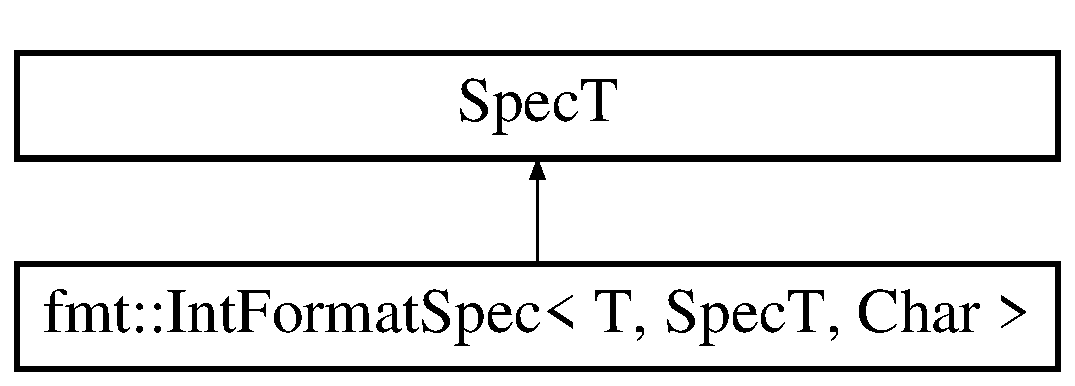
\includegraphics[height=2.000000cm]{classfmt_1_1IntFormatSpec}
\end{center}
\end{figure}
\subsection*{Public Member Functions}
\begin{DoxyCompactItemize}
\item 
{\bfseries Int\+Format\+Spec} (T val, const SpecT \&spec=SpecT())\hypertarget{classfmt_1_1IntFormatSpec_ab3ddcce25115287cbd61e228076d9d8d}{}\label{classfmt_1_1IntFormatSpec_ab3ddcce25115287cbd61e228076d9d8d}

\item 
T {\bfseries value} () const \hypertarget{classfmt_1_1IntFormatSpec_a8d78e074d34780590a4d209e3601947d}{}\label{classfmt_1_1IntFormatSpec_a8d78e074d34780590a4d209e3601947d}

\end{DoxyCompactItemize}


The documentation for this class was generated from the following file\+:\begin{DoxyCompactItemize}
\item 
cvdi-\/src/cvdi-\/cl/include/spdlog/fmt/bundled/format.\+h\end{DoxyCompactItemize}

\hypertarget{structfmt_1_1internal_1_1IntTraits}{}\section{fmt\+:\+:internal\+:\+:Int\+Traits$<$ T $>$ Struct Template Reference}
\label{structfmt_1_1internal_1_1IntTraits}\index{fmt\+::internal\+::\+Int\+Traits$<$ T $>$@{fmt\+::internal\+::\+Int\+Traits$<$ T $>$}}


The documentation for this struct was generated from the following file\+:\begin{DoxyCompactItemize}
\item 
cvdi-\/src/cvdi-\/cl/include/spdlog/fmt/bundled/format.\+h\end{DoxyCompactItemize}

\hypertarget{classgeo__data_1_1KML}{}\section{geo\+\_\+data\+:\+:K\+ML Class Reference}
\label{classgeo__data_1_1KML}\index{geo\+\_\+data\+::\+K\+ML@{geo\+\_\+data\+::\+K\+ML}}


A \hyperlink{classgeo__data_1_1KML}{K\+ML} file.  




{\ttfamily \#include $<$geo\+\_\+data.\+hpp$>$}

\subsection*{Public Types}
\begin{DoxyCompactItemize}
\item 
using {\bfseries Stream\+Ptr} = std\+::shared\+\_\+ptr$<$ std\+::ostream $>$\hypertarget{classgeo__data_1_1KML_a0523f1943a5bdfad5d7c7d707edeec17}{}\label{classgeo__data_1_1KML_a0523f1943a5bdfad5d7c7d707edeec17}

\end{DoxyCompactItemize}
\subsection*{Public Member Functions}
\begin{DoxyCompactItemize}
\item 
\hyperlink{classgeo__data_1_1KML_abcd98547b50dbb378c1a634caa0911e2}{K\+ML} (std\+::ostream \&stream, const std\+::string \&doc\+\_\+name, bool visibility=true)
\begin{DoxyCompactList}\small\item\em Construct a \hyperlink{classgeo__data_1_1KML}{K\+ML} object. \end{DoxyCompactList}\item 
void \hyperlink{classgeo__data_1_1KML_a15aba5605fcae13de084543588d04b65}{finish} ()\hypertarget{classgeo__data_1_1KML_a15aba5605fcae13de084543588d04b65}{}\label{classgeo__data_1_1KML_a15aba5605fcae13de084543588d04b65}

\begin{DoxyCompactList}\small\item\em Finalize the \hyperlink{classgeo__data_1_1KML}{K\+ML} file (write the ending tags). \end{DoxyCompactList}\item 
void \hyperlink{classgeo__data_1_1KML_a52c966b02495f51aac7cbe9ca99a2eec}{write\+\_\+line\+\_\+style} (const std\+::string \&name, unsigned int color\+\_\+value, int width)
\begin{DoxyCompactList}\small\item\em Write a style for a line to the \hyperlink{classgeo__data_1_1KML}{K\+ML} output stream. \end{DoxyCompactList}\item 
void \hyperlink{classgeo__data_1_1KML_a68d10daf35e4c43f024e3e2d2bc44bf2}{write\+\_\+icon\+\_\+style} (const std\+::string \&name, const std\+::string \&href, float scale=1.\+0)
\begin{DoxyCompactList}\small\item\em Write a style for an icon to the \hyperlink{classgeo__data_1_1KML}{K\+ML} output stream. \end{DoxyCompactList}\item 
void \hyperlink{classgeo__data_1_1KML_a2a7e4010226e316d630837ec1f37f7c3}{write\+\_\+poly\+\_\+style} (const std\+::string \&name, unsigned int color\+\_\+value, int width=2, bool fill=true, bool outline=true)
\begin{DoxyCompactList}\small\item\em Write a style for a polygon to the \hyperlink{classgeo__data_1_1KML}{K\+ML} output stream. \end{DoxyCompactList}\item 
void \hyperlink{classgeo__data_1_1KML_a022fed3d67ebd03e5e8b04e27b21ceaf}{write\+\_\+point} (const O\+G\+R\+Point \&point, const std\+::string \&style\+\_\+name)
\begin{DoxyCompactList}\small\item\em Write a single point to the \hyperlink{classgeo__data_1_1KML}{K\+ML} output stream using the point instance. \end{DoxyCompactList}\item 
void \hyperlink{classgeo__data_1_1KML_afce06a5440ba520d2197933c37edc931}{write\+\_\+trace} (const Sample\+::\+Trace \&trace, bool de\+\_\+identify=false, int stride=20)
\begin{DoxyCompactList}\small\item\em Write a rendering of a trajectory to the \hyperlink{classgeo__data_1_1KML}{K\+ML} output stream considering speed and optionally special intervals. The rendering colors points based on the speed of the traveler. Privacy interval points and critical interval points can be excluded. \end{DoxyCompactList}\item 
void \hyperlink{classgeo__data_1_1KML_a1acf0f483bb9a9063e22b665595b7a73}{write\+\_\+intervals} (const Interval\+::\+Ptr\+List \&intervals, const Sample\+::\+Trace \&trace, const std\+::string \&stylename, const std\+::string \&marker\+\_\+style, int stride=10)
\begin{DoxyCompactList}\small\item\em Write the critical and privacy intervals to the \hyperlink{classgeo__data_1_1KML}{K\+ML} output stream. \end{DoxyCompactList}\item 
void \hyperlink{classgeo__data_1_1KML_a59e90e9f806505f53e95910d8133c26d}{write\+\_\+intervals} (const Interval\+::\+Ptr\+List \&intervals, const Sample\+::\+Trace \&trace, const std\+::string \&stylename, int stride=10)
\begin{DoxyCompactList}\small\item\em Write the critical and privacy interavls to the \hyperlink{classgeo__data_1_1KML}{K\+ML} output stream. \end{DoxyCompactList}\item 
void \hyperlink{classgeo__data_1_1KML_aadfd649bf63dfa12f6d90b60e5cc2f81}{write\+\_\+areas} (const std\+::unordered\+\_\+set$<$ geo\+::\+Area\+::\+Ptr $>$ \&aptrset, const std\+::string \&stylename)
\begin{DoxyCompactList}\small\item\em Write a set of \hyperlink{classgeo_1_1Area}{geo\+::\+Area} objects to the \hyperlink{classgeo__data_1_1KML}{K\+ML} output stream. \end{DoxyCompactList}\item 
void \hyperlink{classgeo__data_1_1KML_a687a0d88d709e6b9d6e9f566f80efba7}{write\+\_\+areas} (const std\+::vector$<$ geo\+::\+Area\+::\+Ptr $>$ \&areas, const std\+::string \&stylename)
\begin{DoxyCompactList}\small\item\em Write a vector of \hyperlink{classgeo_1_1Area}{geo\+::\+Area} objects to the \hyperlink{classgeo__data_1_1KML}{K\+ML} output stream. \end{DoxyCompactList}\end{DoxyCompactItemize}
\subsection*{Static Public Attributes}
\begin{DoxyCompactItemize}
\item 
static const double {\bfseries M\+A\+X\+\_\+\+S\+P\+E\+ED} = 36.\+0\hypertarget{classgeo__data_1_1KML_ab44c2f5b2be77eec82125b8c49385a96}{}\label{classgeo__data_1_1KML_ab44c2f5b2be77eec82125b8c49385a96}

\end{DoxyCompactItemize}


\subsection{Detailed Description}
A \hyperlink{classgeo__data_1_1KML}{K\+ML} file. 

\hyperlink{classgeo__data_1_1KML}{K\+ML} Color Values are specified as follows\+: color\+\_\+value is easiest to express in hex\+: 0xaabbggrr where aa -\/$>$ is the transparency alpha. 00 is transparent; ff is fully opaque. where bb -\/$>$ B\+L\+UE where gg -\/$>$ G\+R\+E\+EN where rr -\/$>$ R\+ED This is backwards from how it is usually specified, i.\+e., R\+GB. 

\subsection{Constructor \& Destructor Documentation}
\index{geo\+\_\+data\+::\+K\+ML@{geo\+\_\+data\+::\+K\+ML}!K\+ML@{K\+ML}}
\index{K\+ML@{K\+ML}!geo\+\_\+data\+::\+K\+ML@{geo\+\_\+data\+::\+K\+ML}}
\subsubsection[{\texorpdfstring{K\+M\+L(std\+::ostream \&stream, const std\+::string \&doc\+\_\+name, bool visibility=true)}{KML(std::ostream &stream, const std::string &doc_name, bool visibility=true)}}]{\setlength{\rightskip}{0pt plus 5cm}geo\+\_\+data\+::\+K\+M\+L\+::\+K\+ML (
\begin{DoxyParamCaption}
\item[{std\+::ostream \&}]{stream, }
\item[{const std\+::string \&}]{doc\+\_\+name, }
\item[{bool}]{visibility = {\ttfamily true}}
\end{DoxyParamCaption}
)}\hypertarget{classgeo__data_1_1KML_abcd98547b50dbb378c1a634caa0911e2}{}\label{classgeo__data_1_1KML_abcd98547b50dbb378c1a634caa0911e2}


Construct a \hyperlink{classgeo__data_1_1KML}{K\+ML} object. 


\begin{DoxyParams}{Parameters}
{\em stream} & the output stream to write the \hyperlink{classgeo__data_1_1KML}{K\+ML} \\
\hline
{\em doc\+\_\+name} & the name of the \hyperlink{classgeo__data_1_1KML}{K\+ML} document \\
\hline
{\em visibility} & when true elements will be rendered when the \hyperlink{classgeo__data_1_1KML}{K\+ML} loads \\
\hline
\end{DoxyParams}


\subsection{Member Function Documentation}
\index{geo\+\_\+data\+::\+K\+ML@{geo\+\_\+data\+::\+K\+ML}!write\+\_\+areas@{write\+\_\+areas}}
\index{write\+\_\+areas@{write\+\_\+areas}!geo\+\_\+data\+::\+K\+ML@{geo\+\_\+data\+::\+K\+ML}}
\subsubsection[{\texorpdfstring{write\+\_\+areas(const std\+::unordered\+\_\+set$<$ geo\+::\+Area\+::\+Ptr $>$ \&aptrset, const std\+::string \&stylename)}{write_areas(const std::unordered_set< geo::Area::Ptr > &aptrset, const std::string &stylename)}}]{\setlength{\rightskip}{0pt plus 5cm}void geo\+\_\+data\+::\+K\+M\+L\+::write\+\_\+areas (
\begin{DoxyParamCaption}
\item[{const std\+::unordered\+\_\+set$<$ geo\+::\+Area\+::\+Ptr $>$ \&}]{aptrset, }
\item[{const std\+::string \&}]{stylename}
\end{DoxyParamCaption}
)}\hypertarget{classgeo__data_1_1KML_aadfd649bf63dfa12f6d90b60e5cc2f81}{}\label{classgeo__data_1_1KML_aadfd649bf63dfa12f6d90b60e5cc2f81}


Write a set of \hyperlink{classgeo_1_1Area}{geo\+::\+Area} objects to the \hyperlink{classgeo__data_1_1KML}{K\+ML} output stream. 


\begin{DoxyParams}{Parameters}
{\em aptrset} & the set of areas to render \\
\hline
{\em stylename} & the style to use for the polygon rendering \\
\hline
\end{DoxyParams}
\index{geo\+\_\+data\+::\+K\+ML@{geo\+\_\+data\+::\+K\+ML}!write\+\_\+areas@{write\+\_\+areas}}
\index{write\+\_\+areas@{write\+\_\+areas}!geo\+\_\+data\+::\+K\+ML@{geo\+\_\+data\+::\+K\+ML}}
\subsubsection[{\texorpdfstring{write\+\_\+areas(const std\+::vector$<$ geo\+::\+Area\+::\+Ptr $>$ \&areas, const std\+::string \&stylename)}{write_areas(const std::vector< geo::Area::Ptr > &areas, const std::string &stylename)}}]{\setlength{\rightskip}{0pt plus 5cm}void geo\+\_\+data\+::\+K\+M\+L\+::write\+\_\+areas (
\begin{DoxyParamCaption}
\item[{const std\+::vector$<$ geo\+::\+Area\+::\+Ptr $>$ \&}]{areas, }
\item[{const std\+::string \&}]{stylename}
\end{DoxyParamCaption}
)}\hypertarget{classgeo__data_1_1KML_a687a0d88d709e6b9d6e9f566f80efba7}{}\label{classgeo__data_1_1KML_a687a0d88d709e6b9d6e9f566f80efba7}


Write a vector of \hyperlink{classgeo_1_1Area}{geo\+::\+Area} objects to the \hyperlink{classgeo__data_1_1KML}{K\+ML} output stream. 


\begin{DoxyParams}{Parameters}
{\em areas} & the set of areas to render \\
\hline
{\em stylename} & the style to use for the polygon rendering \\
\hline
\end{DoxyParams}
\index{geo\+\_\+data\+::\+K\+ML@{geo\+\_\+data\+::\+K\+ML}!write\+\_\+icon\+\_\+style@{write\+\_\+icon\+\_\+style}}
\index{write\+\_\+icon\+\_\+style@{write\+\_\+icon\+\_\+style}!geo\+\_\+data\+::\+K\+ML@{geo\+\_\+data\+::\+K\+ML}}
\subsubsection[{\texorpdfstring{write\+\_\+icon\+\_\+style(const std\+::string \&name, const std\+::string \&href, float scale=1.\+0)}{write_icon_style(const std::string &name, const std::string &href, float scale=1.0)}}]{\setlength{\rightskip}{0pt plus 5cm}void geo\+\_\+data\+::\+K\+M\+L\+::write\+\_\+icon\+\_\+style (
\begin{DoxyParamCaption}
\item[{const std\+::string \&}]{name, }
\item[{const std\+::string \&}]{href, }
\item[{float}]{scale = {\ttfamily 1.0}}
\end{DoxyParamCaption}
)}\hypertarget{classgeo__data_1_1KML_a68d10daf35e4c43f024e3e2d2bc44bf2}{}\label{classgeo__data_1_1KML_a68d10daf35e4c43f024e3e2d2bc44bf2}


Write a style for an icon to the \hyperlink{classgeo__data_1_1KML}{K\+ML} output stream. 


\begin{DoxyParams}{Parameters}
{\em name} & the style ID \\
\hline
{\em href} & the U\+RL for the icon graphic \\
\hline
{\em scale} & the size adjustment of the icon relative to its original size \\
\hline
\end{DoxyParams}
\index{geo\+\_\+data\+::\+K\+ML@{geo\+\_\+data\+::\+K\+ML}!write\+\_\+intervals@{write\+\_\+intervals}}
\index{write\+\_\+intervals@{write\+\_\+intervals}!geo\+\_\+data\+::\+K\+ML@{geo\+\_\+data\+::\+K\+ML}}
\subsubsection[{\texorpdfstring{write\+\_\+intervals(const Interval\+::\+Ptr\+List \&intervals, const Sample\+::\+Trace \&trace, const std\+::string \&stylename, const std\+::string \&marker\+\_\+style, int stride=10)}{write_intervals(const Interval::PtrList &intervals, const Sample::Trace &trace, const std::string &stylename, const std::string &marker_style, int stride=10)}}]{\setlength{\rightskip}{0pt plus 5cm}void geo\+\_\+data\+::\+K\+M\+L\+::write\+\_\+intervals (
\begin{DoxyParamCaption}
\item[{const Interval\+::\+Ptr\+List \&}]{intervals, }
\item[{const Sample\+::\+Trace \&}]{trace, }
\item[{const std\+::string \&}]{stylename, }
\item[{const std\+::string \&}]{marker\+\_\+style, }
\item[{int}]{stride = {\ttfamily 10}}
\end{DoxyParamCaption}
)}\hypertarget{classgeo__data_1_1KML_a1acf0f483bb9a9063e22b665595b7a73}{}\label{classgeo__data_1_1KML_a1acf0f483bb9a9063e22b665595b7a73}


Write the critical and privacy intervals to the \hyperlink{classgeo__data_1_1KML}{K\+ML} output stream. 

The intervals contain indexes into the provided trajectory.


\begin{DoxyParams}{Parameters}
{\em intervals} & the list of intervals to render in the \hyperlink{classgeo__data_1_1KML}{K\+ML} \\
\hline
{\em trace} & the trace that generated the intervals \\
\hline
{\em stylename} & the style ID for the interval trip points \\
\hline
{\em marker\+\_\+style} & the style ID to use for the first point in the interval (highlights the interval type or what triggered it) \\
\hline
{\em stride} & the number of trip points to skip to minimize the amount of data rendered \\
\hline
\end{DoxyParams}
\index{geo\+\_\+data\+::\+K\+ML@{geo\+\_\+data\+::\+K\+ML}!write\+\_\+intervals@{write\+\_\+intervals}}
\index{write\+\_\+intervals@{write\+\_\+intervals}!geo\+\_\+data\+::\+K\+ML@{geo\+\_\+data\+::\+K\+ML}}
\subsubsection[{\texorpdfstring{write\+\_\+intervals(const Interval\+::\+Ptr\+List \&intervals, const Sample\+::\+Trace \&trace, const std\+::string \&stylename, int stride=10)}{write_intervals(const Interval::PtrList &intervals, const Sample::Trace &trace, const std::string &stylename, int stride=10)}}]{\setlength{\rightskip}{0pt plus 5cm}void geo\+\_\+data\+::\+K\+M\+L\+::write\+\_\+intervals (
\begin{DoxyParamCaption}
\item[{const Interval\+::\+Ptr\+List \&}]{intervals, }
\item[{const Sample\+::\+Trace \&}]{trace, }
\item[{const std\+::string \&}]{stylename, }
\item[{int}]{stride = {\ttfamily 10}}
\end{DoxyParamCaption}
)}\hypertarget{classgeo__data_1_1KML_a59e90e9f806505f53e95910d8133c26d}{}\label{classgeo__data_1_1KML_a59e90e9f806505f53e95910d8133c26d}


Write the critical and privacy interavls to the \hyperlink{classgeo__data_1_1KML}{K\+ML} output stream. 

The intervals contain indexes into the provided trajectory. This method does N\+OT mark the first point in the interval.


\begin{DoxyParams}{Parameters}
{\em intervals} & the list of intervals to render in the \hyperlink{classgeo__data_1_1KML}{K\+ML} \\
\hline
{\em traj} & the trajectory that generated the intervals \\
\hline
{\em stylename} & the style ID for the interval sample points \\
\hline
{\em stride} & the number of trip points to skip to minimize the amount of data rendered \\
\hline
\end{DoxyParams}
\index{geo\+\_\+data\+::\+K\+ML@{geo\+\_\+data\+::\+K\+ML}!write\+\_\+line\+\_\+style@{write\+\_\+line\+\_\+style}}
\index{write\+\_\+line\+\_\+style@{write\+\_\+line\+\_\+style}!geo\+\_\+data\+::\+K\+ML@{geo\+\_\+data\+::\+K\+ML}}
\subsubsection[{\texorpdfstring{write\+\_\+line\+\_\+style(const std\+::string \&name, unsigned int color\+\_\+value, int width)}{write_line_style(const std::string &name, unsigned int color_value, int width)}}]{\setlength{\rightskip}{0pt plus 5cm}void geo\+\_\+data\+::\+K\+M\+L\+::write\+\_\+line\+\_\+style (
\begin{DoxyParamCaption}
\item[{const std\+::string \&}]{name, }
\item[{unsigned int}]{color\+\_\+value, }
\item[{int}]{width}
\end{DoxyParamCaption}
)}\hypertarget{classgeo__data_1_1KML_a52c966b02495f51aac7cbe9ca99a2eec}{}\label{classgeo__data_1_1KML_a52c966b02495f51aac7cbe9ca99a2eec}


Write a style for a line to the \hyperlink{classgeo__data_1_1KML}{K\+ML} output stream. 


\begin{DoxyParams}{Parameters}
{\em name} & the style ID \\
\hline
{\em color\+\_\+value} & the \hyperlink{classgeo__data_1_1KML}{K\+ML} color value as an integer (will be converted to hex) \\
\hline
{\em width} & the width of the line in pixels \\
\hline
\end{DoxyParams}
\index{geo\+\_\+data\+::\+K\+ML@{geo\+\_\+data\+::\+K\+ML}!write\+\_\+point@{write\+\_\+point}}
\index{write\+\_\+point@{write\+\_\+point}!geo\+\_\+data\+::\+K\+ML@{geo\+\_\+data\+::\+K\+ML}}
\subsubsection[{\texorpdfstring{write\+\_\+point(const O\+G\+R\+Point \&point, const std\+::string \&style\+\_\+name)}{write_point(const OGRPoint &point, const std::string &style_name)}}]{\setlength{\rightskip}{0pt plus 5cm}void geo\+\_\+data\+::\+K\+M\+L\+::write\+\_\+point (
\begin{DoxyParamCaption}
\item[{const O\+G\+R\+Point \&}]{point, }
\item[{const std\+::string \&}]{style\+\_\+name}
\end{DoxyParamCaption}
)}\hypertarget{classgeo__data_1_1KML_a022fed3d67ebd03e5e8b04e27b21ceaf}{}\label{classgeo__data_1_1KML_a022fed3d67ebd03e5e8b04e27b21ceaf}


Write a single point to the \hyperlink{classgeo__data_1_1KML}{K\+ML} output stream using the point instance. 


\begin{DoxyParams}{Parameters}
{\em point} & the point to represent in \hyperlink{classgeo__data_1_1KML}{K\+ML} \\
\hline
{\em style\+\_\+name} & the ID of the style for the point \\
\hline
\end{DoxyParams}
\index{geo\+\_\+data\+::\+K\+ML@{geo\+\_\+data\+::\+K\+ML}!write\+\_\+poly\+\_\+style@{write\+\_\+poly\+\_\+style}}
\index{write\+\_\+poly\+\_\+style@{write\+\_\+poly\+\_\+style}!geo\+\_\+data\+::\+K\+ML@{geo\+\_\+data\+::\+K\+ML}}
\subsubsection[{\texorpdfstring{write\+\_\+poly\+\_\+style(const std\+::string \&name, unsigned int color\+\_\+value, int width=2, bool fill=true, bool outline=true)}{write_poly_style(const std::string &name, unsigned int color_value, int width=2, bool fill=true, bool outline=true)}}]{\setlength{\rightskip}{0pt plus 5cm}void geo\+\_\+data\+::\+K\+M\+L\+::write\+\_\+poly\+\_\+style (
\begin{DoxyParamCaption}
\item[{const std\+::string \&}]{name, }
\item[{unsigned int}]{color\+\_\+value, }
\item[{int}]{width = {\ttfamily 2}, }
\item[{bool}]{fill = {\ttfamily true}, }
\item[{bool}]{outline = {\ttfamily true}}
\end{DoxyParamCaption}
)}\hypertarget{classgeo__data_1_1KML_a2a7e4010226e316d630837ec1f37f7c3}{}\label{classgeo__data_1_1KML_a2a7e4010226e316d630837ec1f37f7c3}


Write a style for a polygon to the \hyperlink{classgeo__data_1_1KML}{K\+ML} output stream. 


\begin{DoxyParams}{Parameters}
{\em name} & the style ID \\
\hline
{\em color\+\_\+value} & the \hyperlink{classgeo__data_1_1KML}{K\+ML} color value as an integer (will be converted to hex) \\
\hline
{\em width} & the width of the line in pixels \\
\hline
{\em fill} & true indicates the polygon should be color filled \\
\hline
{\em outline} & true indicates the polygon should be outlined \\
\hline
\end{DoxyParams}
\index{geo\+\_\+data\+::\+K\+ML@{geo\+\_\+data\+::\+K\+ML}!write\+\_\+trace@{write\+\_\+trace}}
\index{write\+\_\+trace@{write\+\_\+trace}!geo\+\_\+data\+::\+K\+ML@{geo\+\_\+data\+::\+K\+ML}}
\subsubsection[{\texorpdfstring{write\+\_\+trace(const Sample\+::\+Trace \&trace, bool de\+\_\+identify=false, int stride=20)}{write_trace(const Sample::Trace &trace, bool de_identify=false, int stride=20)}}]{\setlength{\rightskip}{0pt plus 5cm}void geo\+\_\+data\+::\+K\+M\+L\+::write\+\_\+trace (
\begin{DoxyParamCaption}
\item[{const Sample\+::\+Trace \&}]{trace, }
\item[{bool}]{de\+\_\+identify = {\ttfamily false}, }
\item[{int}]{stride = {\ttfamily 20}}
\end{DoxyParamCaption}
)}\hypertarget{classgeo__data_1_1KML_afce06a5440ba520d2197933c37edc931}{}\label{classgeo__data_1_1KML_afce06a5440ba520d2197933c37edc931}


Write a rendering of a trajectory to the \hyperlink{classgeo__data_1_1KML}{K\+ML} output stream considering speed and optionally special intervals. The rendering colors points based on the speed of the traveler. Privacy interval points and critical interval points can be excluded. 


\begin{DoxyParams}{Parameters}
{\em trace} & the trace to base the line on \\
\hline
{\em de\+\_\+identify} & flag to suppress the privacy and critical intervals \\
\hline
{\em stride} & the number of trajectory points to skip while rendering the line as a sequence of segments \\
\hline
\end{DoxyParams}


The documentation for this class was generated from the following files\+:\begin{DoxyCompactItemize}
\item 
cvdi-\/src/geo-\/data/include/geo\+\_\+data.\+hpp\item 
cvdi-\/src/geo-\/data/src/geo\+\_\+data.\+cpp\end{DoxyCompactItemize}

\hypertarget{structfmt_1_1internal_1_1LConvCheck}{}\section{fmt\+:\+:internal\+:\+:L\+Conv\+Check$<$ T, T $>$ Struct Template Reference}
\label{structfmt_1_1internal_1_1LConvCheck}\index{fmt\+::internal\+::\+L\+Conv\+Check$<$ T, T $>$@{fmt\+::internal\+::\+L\+Conv\+Check$<$ T, T $>$}}
\subsection*{Public Member Functions}
\begin{DoxyCompactItemize}
\item 
{\bfseries L\+Conv\+Check} (int)\hypertarget{structfmt_1_1internal_1_1LConvCheck_af5a35a7bced670df56dcef11f37d1427}{}\label{structfmt_1_1internal_1_1LConvCheck_af5a35a7bced670df56dcef11f37d1427}

\end{DoxyCompactItemize}


The documentation for this struct was generated from the following file\+:\begin{DoxyCompactItemize}
\item 
cvdi-\/src/cvdi-\/cl/include/spdlog/fmt/bundled/format.\+h\end{DoxyCompactItemize}

\hypertarget{classspdlog_1_1details_1_1level__formatter}{}\section{spdlog\+:\+:details\+:\+:level\+\_\+formatter Class Reference}
\label{classspdlog_1_1details_1_1level__formatter}\index{spdlog\+::details\+::level\+\_\+formatter@{spdlog\+::details\+::level\+\_\+formatter}}
Inheritance diagram for spdlog\+:\+:details\+:\+:level\+\_\+formatter\+:\begin{figure}[H]
\begin{center}
\leavevmode
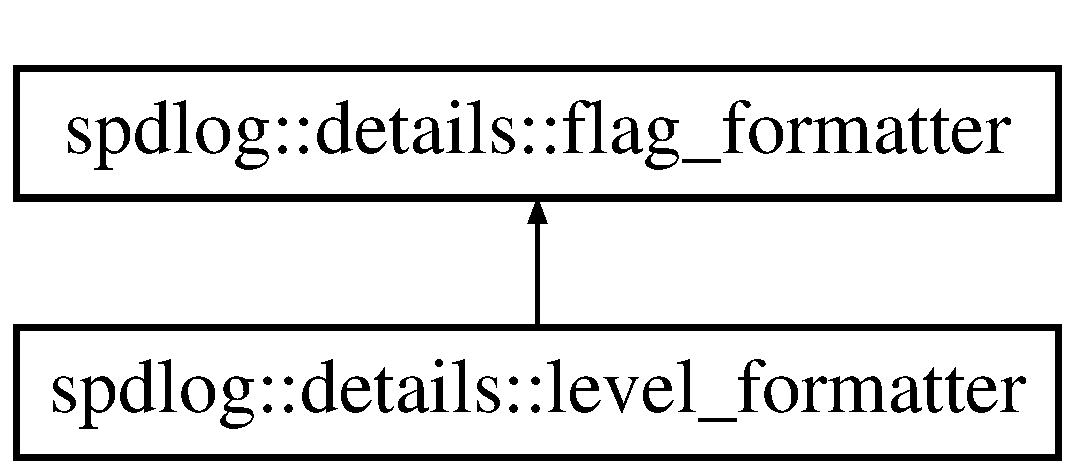
\includegraphics[height=2.000000cm]{classspdlog_1_1details_1_1level__formatter}
\end{center}
\end{figure}
\subsection*{Additional Inherited Members}


The documentation for this class was generated from the following file\+:\begin{DoxyCompactItemize}
\item 
cvdi-\/src/cvdi-\/cl/include/spdlog/details/pattern\+\_\+formatter\+\_\+impl.\+h\end{DoxyCompactItemize}

\hypertarget{structspdlog_1_1details_1_1log__msg}{}\section{spdlog\+:\+:details\+:\+:log\+\_\+msg Struct Reference}
\label{structspdlog_1_1details_1_1log__msg}\index{spdlog\+::details\+::log\+\_\+msg@{spdlog\+::details\+::log\+\_\+msg}}
\subsection*{Public Member Functions}
\begin{DoxyCompactItemize}
\item 
{\bfseries log\+\_\+msg} (const std\+::string $\ast$loggers\+\_\+name, level\+::level\+\_\+enum lvl)\hypertarget{structspdlog_1_1details_1_1log__msg_a70dc787cddfaf8e678f0fa135a4e5525}{}\label{structspdlog_1_1details_1_1log__msg_a70dc787cddfaf8e678f0fa135a4e5525}

\item 
{\bfseries log\+\_\+msg} (const \hyperlink{structspdlog_1_1details_1_1log__msg}{log\+\_\+msg} \&other)=delete\hypertarget{structspdlog_1_1details_1_1log__msg_a51f3ba00f2c47f37ed2a4692c8b028b2}{}\label{structspdlog_1_1details_1_1log__msg_a51f3ba00f2c47f37ed2a4692c8b028b2}

\item 
\hyperlink{structspdlog_1_1details_1_1log__msg}{log\+\_\+msg} \& {\bfseries operator=} (\hyperlink{structspdlog_1_1details_1_1log__msg}{log\+\_\+msg} \&\&other)=delete\hypertarget{structspdlog_1_1details_1_1log__msg_a48a0c8c70f176b915487ec4511781c46}{}\label{structspdlog_1_1details_1_1log__msg_a48a0c8c70f176b915487ec4511781c46}

\item 
{\bfseries log\+\_\+msg} (\hyperlink{structspdlog_1_1details_1_1log__msg}{log\+\_\+msg} \&\&other)=delete\hypertarget{structspdlog_1_1details_1_1log__msg_aaedee42f7e295700b9ad8a5378997a70}{}\label{structspdlog_1_1details_1_1log__msg_aaedee42f7e295700b9ad8a5378997a70}

\end{DoxyCompactItemize}
\subsection*{Public Attributes}
\begin{DoxyCompactItemize}
\item 
const std\+::string $\ast$ {\bfseries logger\+\_\+name}\hypertarget{structspdlog_1_1details_1_1log__msg_a0aacbf01e2a67660d328fa2080d55def}{}\label{structspdlog_1_1details_1_1log__msg_a0aacbf01e2a67660d328fa2080d55def}

\item 
level\+::level\+\_\+enum {\bfseries level}\hypertarget{structspdlog_1_1details_1_1log__msg_a4142f4d66140a1ea24053311ebea5706}{}\label{structspdlog_1_1details_1_1log__msg_a4142f4d66140a1ea24053311ebea5706}

\item 
log\+\_\+clock\+::time\+\_\+point {\bfseries time}\hypertarget{structspdlog_1_1details_1_1log__msg_a25fadb26e6ce94657af5475d4a581313}{}\label{structspdlog_1_1details_1_1log__msg_a25fadb26e6ce94657af5475d4a581313}

\item 
size\+\_\+t {\bfseries thread\+\_\+id}\hypertarget{structspdlog_1_1details_1_1log__msg_ab8474cd689276f61021bca37e1993eef}{}\label{structspdlog_1_1details_1_1log__msg_ab8474cd689276f61021bca37e1993eef}

\item 
\hyperlink{classfmt_1_1BasicMemoryWriter}{fmt\+::\+Memory\+Writer} {\bfseries raw}\hypertarget{structspdlog_1_1details_1_1log__msg_a4408eab696be1086d11e351184ecc68c}{}\label{structspdlog_1_1details_1_1log__msg_a4408eab696be1086d11e351184ecc68c}

\item 
\hyperlink{classfmt_1_1BasicMemoryWriter}{fmt\+::\+Memory\+Writer} {\bfseries formatted}\hypertarget{structspdlog_1_1details_1_1log__msg_a20b83810adf6cfaf73fd2e7b42c3016c}{}\label{structspdlog_1_1details_1_1log__msg_a20b83810adf6cfaf73fd2e7b42c3016c}

\item 
size\+\_\+t {\bfseries msg\+\_\+id}\hypertarget{structspdlog_1_1details_1_1log__msg_a8cbec91cdecd3cb4efe9cfa39d5d1d84}{}\label{structspdlog_1_1details_1_1log__msg_a8cbec91cdecd3cb4efe9cfa39d5d1d84}

\end{DoxyCompactItemize}


The documentation for this struct was generated from the following file\+:\begin{DoxyCompactItemize}
\item 
cvdi-\/src/cvdi-\/cl/include/spdlog/details/log\+\_\+msg.\+h\end{DoxyCompactItemize}

\hypertarget{classspdlog_1_1logger}{}\section{spdlog\+:\+:logger Class Reference}
\label{classspdlog_1_1logger}\index{spdlog\+::logger@{spdlog\+::logger}}
Inheritance diagram for spdlog\+:\+:logger\+:\begin{figure}[H]
\begin{center}
\leavevmode
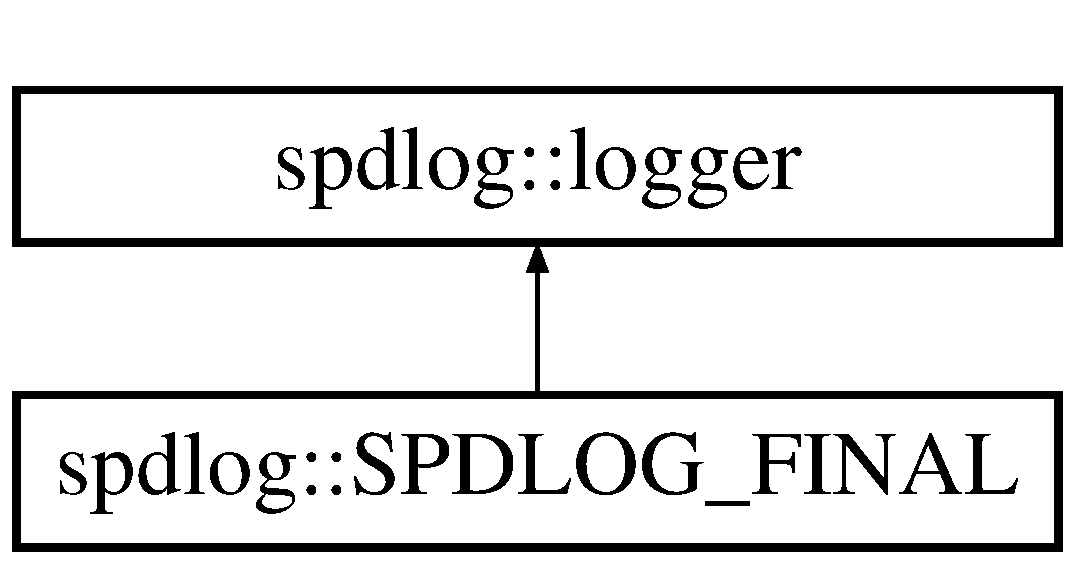
\includegraphics[height=2.000000cm]{classspdlog_1_1logger}
\end{center}
\end{figure}
\subsection*{Public Member Functions}
\begin{DoxyCompactItemize}
\item 
{\bfseries logger} (const std\+::string \&logger\+\_\+name, sink\+\_\+ptr single\+\_\+sink)\hypertarget{classspdlog_1_1logger_a01e952f5adbc10326c3d77b3ded7063b}{}\label{classspdlog_1_1logger_a01e952f5adbc10326c3d77b3ded7063b}

\item 
{\bfseries logger} (const std\+::string \&name, sinks\+\_\+init\+\_\+list)\hypertarget{classspdlog_1_1logger_a1c4b03a1b5d3a2305e19aee47f8f2c17}{}\label{classspdlog_1_1logger_a1c4b03a1b5d3a2305e19aee47f8f2c17}

\item 
{\footnotesize template$<$class It $>$ }\\{\bfseries logger} (const std\+::string \&name, const It \&begin, const It \&end)\hypertarget{classspdlog_1_1logger_add870b09f8a36ee6660cc0dc4eba258a}{}\label{classspdlog_1_1logger_add870b09f8a36ee6660cc0dc4eba258a}

\item 
{\bfseries logger} (const \hyperlink{classspdlog_1_1logger}{logger} \&)=delete\hypertarget{classspdlog_1_1logger_aa6074d763b0df4e7d16ccf7d307a3938}{}\label{classspdlog_1_1logger_aa6074d763b0df4e7d16ccf7d307a3938}

\item 
\hyperlink{classspdlog_1_1logger}{logger} \& {\bfseries operator=} (const \hyperlink{classspdlog_1_1logger}{logger} \&)=delete\hypertarget{classspdlog_1_1logger_afd373cd857f49de170d9a23f1dd34bc0}{}\label{classspdlog_1_1logger_afd373cd857f49de170d9a23f1dd34bc0}

\item 
{\footnotesize template$<$typename... Args$>$ }\\void {\bfseries log} (level\+::level\+\_\+enum lvl, const char $\ast$fmt, const Args \&...args)\hypertarget{classspdlog_1_1logger_a5149c7b8c1ac8aeedbeba779b0e0cfb7}{}\label{classspdlog_1_1logger_a5149c7b8c1ac8aeedbeba779b0e0cfb7}

\item 
{\footnotesize template$<$typename... Args$>$ }\\void {\bfseries log} (level\+::level\+\_\+enum lvl, const char $\ast$msg)\hypertarget{classspdlog_1_1logger_a44da1d3a0003e6a67fddb3d7bb99ce1d}{}\label{classspdlog_1_1logger_a44da1d3a0003e6a67fddb3d7bb99ce1d}

\item 
{\footnotesize template$<$typename Arg1 , typename... Args$>$ }\\void {\bfseries trace} (const char $\ast$fmt, const Arg1 \&, const Args \&...args)\hypertarget{classspdlog_1_1logger_aa580734685da694da3d17d43232ec3ac}{}\label{classspdlog_1_1logger_aa580734685da694da3d17d43232ec3ac}

\item 
{\footnotesize template$<$typename Arg1 , typename... Args$>$ }\\void {\bfseries debug} (const char $\ast$fmt, const Arg1 \&, const Args \&...args)\hypertarget{classspdlog_1_1logger_af814a11eca93b3a173f3da389f5f751b}{}\label{classspdlog_1_1logger_af814a11eca93b3a173f3da389f5f751b}

\item 
{\footnotesize template$<$typename Arg1 , typename... Args$>$ }\\void {\bfseries info} (const char $\ast$fmt, const Arg1 \&, const Args \&...args)\hypertarget{classspdlog_1_1logger_abbc0dd1cd95139acebe5ed0cc003ec16}{}\label{classspdlog_1_1logger_abbc0dd1cd95139acebe5ed0cc003ec16}

\item 
{\footnotesize template$<$typename Arg1 , typename... Args$>$ }\\void {\bfseries warn} (const char $\ast$fmt, const Arg1 \&, const Args \&...args)\hypertarget{classspdlog_1_1logger_a04c38de2bcde8fa35d56f136988bf338}{}\label{classspdlog_1_1logger_a04c38de2bcde8fa35d56f136988bf338}

\item 
{\footnotesize template$<$typename Arg1 , typename... Args$>$ }\\void {\bfseries error} (const char $\ast$fmt, const Arg1 \&, const Args \&...args)\hypertarget{classspdlog_1_1logger_aadc2f59f010c7d7140e1d90900d7888e}{}\label{classspdlog_1_1logger_aadc2f59f010c7d7140e1d90900d7888e}

\item 
{\footnotesize template$<$typename Arg1 , typename... Args$>$ }\\void {\bfseries critical} (const char $\ast$fmt, const Arg1 \&, const Args \&...args)\hypertarget{classspdlog_1_1logger_a3dbacca444787282fb94bf2c79f48fef}{}\label{classspdlog_1_1logger_a3dbacca444787282fb94bf2c79f48fef}

\item 
{\footnotesize template$<$typename T $>$ }\\void {\bfseries log} (level\+::level\+\_\+enum lvl, const T \&)\hypertarget{classspdlog_1_1logger_a16d3d178ac86ea71b8a0becfca0c5449}{}\label{classspdlog_1_1logger_a16d3d178ac86ea71b8a0becfca0c5449}

\item 
{\footnotesize template$<$typename T $>$ }\\void {\bfseries trace} (const T \&)\hypertarget{classspdlog_1_1logger_a8d0c37f6eb65405b7dcfc7e7d60e6e58}{}\label{classspdlog_1_1logger_a8d0c37f6eb65405b7dcfc7e7d60e6e58}

\item 
{\footnotesize template$<$typename T $>$ }\\void {\bfseries debug} (const T \&)\hypertarget{classspdlog_1_1logger_ab46aca3267a2f2c4bfc25834067527e0}{}\label{classspdlog_1_1logger_ab46aca3267a2f2c4bfc25834067527e0}

\item 
{\footnotesize template$<$typename T $>$ }\\void {\bfseries info} (const T \&)\hypertarget{classspdlog_1_1logger_af002a28bd29ef0f798ca67191419b129}{}\label{classspdlog_1_1logger_af002a28bd29ef0f798ca67191419b129}

\item 
{\footnotesize template$<$typename T $>$ }\\void {\bfseries warn} (const T \&)\hypertarget{classspdlog_1_1logger_a7b4abd6d315181b2421e89f0efe71743}{}\label{classspdlog_1_1logger_a7b4abd6d315181b2421e89f0efe71743}

\item 
{\footnotesize template$<$typename T $>$ }\\void {\bfseries error} (const T \&)\hypertarget{classspdlog_1_1logger_aa91ef7020d423cf399fb54ae7800964f}{}\label{classspdlog_1_1logger_aa91ef7020d423cf399fb54ae7800964f}

\item 
{\footnotesize template$<$typename T $>$ }\\void {\bfseries critical} (const T \&)\hypertarget{classspdlog_1_1logger_a3102470f39f6d84e083e62d9c336fecd}{}\label{classspdlog_1_1logger_a3102470f39f6d84e083e62d9c336fecd}

\item 
bool {\bfseries should\+\_\+log} (level\+::level\+\_\+enum) const \hypertarget{classspdlog_1_1logger_a6c0941a0897874e3c7c3cc77edafa13e}{}\label{classspdlog_1_1logger_a6c0941a0897874e3c7c3cc77edafa13e}

\item 
void {\bfseries set\+\_\+level} (level\+::level\+\_\+enum)\hypertarget{classspdlog_1_1logger_afa83b0334d1599dd148f14ed4b8bae9f}{}\label{classspdlog_1_1logger_afa83b0334d1599dd148f14ed4b8bae9f}

\item 
level\+::level\+\_\+enum {\bfseries level} () const \hypertarget{classspdlog_1_1logger_a6fdaf38b46b34772ffa728e8faa3e857}{}\label{classspdlog_1_1logger_a6fdaf38b46b34772ffa728e8faa3e857}

\item 
const std\+::string \& {\bfseries name} () const \hypertarget{classspdlog_1_1logger_a965147f4736d658065f8ba6e923c1c47}{}\label{classspdlog_1_1logger_a965147f4736d658065f8ba6e923c1c47}

\item 
void {\bfseries set\+\_\+pattern} (const std\+::string \&, pattern\+\_\+time\+\_\+type=pattern\+\_\+time\+\_\+type\+::local)\hypertarget{classspdlog_1_1logger_a7fef08e7bfc1369e31f5cf1f0b213be2}{}\label{classspdlog_1_1logger_a7fef08e7bfc1369e31f5cf1f0b213be2}

\item 
void {\bfseries set\+\_\+formatter} (formatter\+\_\+ptr)\hypertarget{classspdlog_1_1logger_a5671bc1118ec7486591e288518b7854f}{}\label{classspdlog_1_1logger_a5671bc1118ec7486591e288518b7854f}

\item 
void {\bfseries flush\+\_\+on} (level\+::level\+\_\+enum log\+\_\+level)\hypertarget{classspdlog_1_1logger_a47c021d339c1f246758e1a87a41668e3}{}\label{classspdlog_1_1logger_a47c021d339c1f246758e1a87a41668e3}

\item 
virtual void {\bfseries flush} ()\hypertarget{classspdlog_1_1logger_a861bb4d4e65de07966148822075bee86}{}\label{classspdlog_1_1logger_a861bb4d4e65de07966148822075bee86}

\item 
const std\+::vector$<$ sink\+\_\+ptr $>$ \& {\bfseries sinks} () const \hypertarget{classspdlog_1_1logger_a59a64487a6c9714d2f7c70b5e094711b}{}\label{classspdlog_1_1logger_a59a64487a6c9714d2f7c70b5e094711b}

\item 
virtual void {\bfseries set\+\_\+error\+\_\+handler} (log\+\_\+err\+\_\+handler)\hypertarget{classspdlog_1_1logger_a7f20aa1910f281f3fd8e477d165ee124}{}\label{classspdlog_1_1logger_a7f20aa1910f281f3fd8e477d165ee124}

\item 
virtual log\+\_\+err\+\_\+handler {\bfseries error\+\_\+handler} ()\hypertarget{classspdlog_1_1logger_a49f6b60692fdaf3adfc13f9831c4bd14}{}\label{classspdlog_1_1logger_a49f6b60692fdaf3adfc13f9831c4bd14}

\end{DoxyCompactItemize}
\subsection*{Protected Member Functions}
\begin{DoxyCompactItemize}
\item 
virtual void {\bfseries \+\_\+sink\+\_\+it} (\hyperlink{structspdlog_1_1details_1_1log__msg}{details\+::log\+\_\+msg} \&)\hypertarget{classspdlog_1_1logger_ace111ec67a09bca55fa8f73233b79b08}{}\label{classspdlog_1_1logger_ace111ec67a09bca55fa8f73233b79b08}

\item 
virtual void {\bfseries \+\_\+set\+\_\+pattern} (const std\+::string \&, pattern\+\_\+time\+\_\+type)\hypertarget{classspdlog_1_1logger_a1bdb98068fca139a50a167894bc7fcd0}{}\label{classspdlog_1_1logger_a1bdb98068fca139a50a167894bc7fcd0}

\item 
virtual void {\bfseries \+\_\+set\+\_\+formatter} (formatter\+\_\+ptr)\hypertarget{classspdlog_1_1logger_addb8fd1eec5a87bcfa8cec1ab32aa375}{}\label{classspdlog_1_1logger_addb8fd1eec5a87bcfa8cec1ab32aa375}

\item 
virtual void {\bfseries \+\_\+default\+\_\+err\+\_\+handler} (const std\+::string \&msg)\hypertarget{classspdlog_1_1logger_a3a4a00fbf7e739dcd162ef4a5a98fb56}{}\label{classspdlog_1_1logger_a3a4a00fbf7e739dcd162ef4a5a98fb56}

\item 
bool {\bfseries \+\_\+should\+\_\+flush\+\_\+on} (const \hyperlink{structspdlog_1_1details_1_1log__msg}{details\+::log\+\_\+msg} \&)\hypertarget{classspdlog_1_1logger_ab6905b5e7a19a319d65682bdc859373a}{}\label{classspdlog_1_1logger_ab6905b5e7a19a319d65682bdc859373a}

\end{DoxyCompactItemize}
\subsection*{Protected Attributes}
\begin{DoxyCompactItemize}
\item 
const std\+::string {\bfseries \+\_\+name}\hypertarget{classspdlog_1_1logger_a819e97be3b6e2066edb7798c04121749}{}\label{classspdlog_1_1logger_a819e97be3b6e2066edb7798c04121749}

\item 
std\+::vector$<$ sink\+\_\+ptr $>$ {\bfseries \+\_\+sinks}\hypertarget{classspdlog_1_1logger_aa3563923d7afee42f8ae19e5b1a6daea}{}\label{classspdlog_1_1logger_aa3563923d7afee42f8ae19e5b1a6daea}

\item 
formatter\+\_\+ptr {\bfseries \+\_\+formatter}\hypertarget{classspdlog_1_1logger_af3d364c4242d9071f9f7d48e437c373f}{}\label{classspdlog_1_1logger_af3d364c4242d9071f9f7d48e437c373f}

\item 
spdlog\+::level\+\_\+t {\bfseries \+\_\+level}\hypertarget{classspdlog_1_1logger_a89f596c2328f2ce5402c77eb8b181ab6}{}\label{classspdlog_1_1logger_a89f596c2328f2ce5402c77eb8b181ab6}

\item 
spdlog\+::level\+\_\+t {\bfseries \+\_\+flush\+\_\+level}\hypertarget{classspdlog_1_1logger_a53dcc290a397bd019756cfedf4d839d2}{}\label{classspdlog_1_1logger_a53dcc290a397bd019756cfedf4d839d2}

\item 
log\+\_\+err\+\_\+handler {\bfseries \+\_\+err\+\_\+handler}\hypertarget{classspdlog_1_1logger_a249eaef178568d6f7153e33118f8a9da}{}\label{classspdlog_1_1logger_a249eaef178568d6f7153e33118f8a9da}

\item 
std\+::atomic$<$ time\+\_\+t $>$ {\bfseries \+\_\+last\+\_\+err\+\_\+time}\hypertarget{classspdlog_1_1logger_a0b88740c53e5fc64ebebdbbd1640a4a6}{}\label{classspdlog_1_1logger_a0b88740c53e5fc64ebebdbbd1640a4a6}

\item 
std\+::atomic$<$ size\+\_\+t $>$ {\bfseries \+\_\+msg\+\_\+counter}\hypertarget{classspdlog_1_1logger_ab0f217552f160a7154a4398bcec65263}{}\label{classspdlog_1_1logger_ab0f217552f160a7154a4398bcec65263}

\end{DoxyCompactItemize}


The documentation for this class was generated from the following files\+:\begin{DoxyCompactItemize}
\item 
cvdi-\/src/cvdi-\/cl/include/spdlog/logger.\+h\item 
cvdi-\/src/cvdi-\/cl/include/spdlog/details/logger\+\_\+impl.\+h\end{DoxyCompactItemize}

\hypertarget{classfmt_1_1internal_1_1MakeArg}{}\section{fmt\+:\+:internal\+:\+:Make\+Arg$<$ Formatter $>$ Class Template Reference}
\label{classfmt_1_1internal_1_1MakeArg}\index{fmt\+::internal\+::\+Make\+Arg$<$ Formatter $>$@{fmt\+::internal\+::\+Make\+Arg$<$ Formatter $>$}}
Inheritance diagram for fmt\+:\+:internal\+:\+:Make\+Arg$<$ Formatter $>$\+:\begin{figure}[H]
\begin{center}
\leavevmode
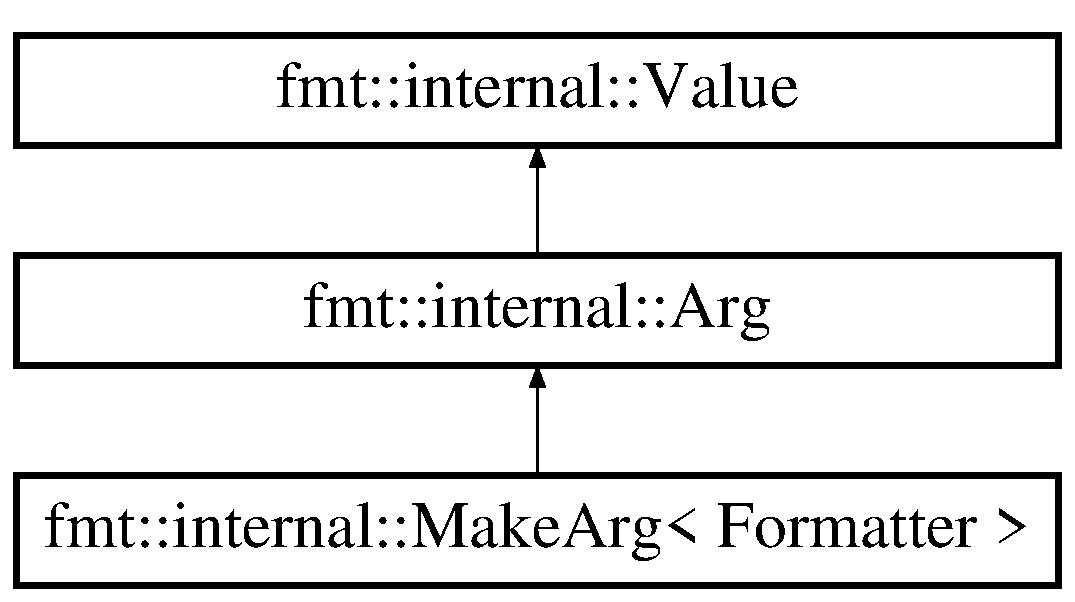
\includegraphics[height=3.000000cm]{classfmt_1_1internal_1_1MakeArg}
\end{center}
\end{figure}
\subsection*{Public Member Functions}
\begin{DoxyCompactItemize}
\item 
{\footnotesize template$<$typename T $>$ }\\{\bfseries Make\+Arg} (const T \&value)\hypertarget{classfmt_1_1internal_1_1MakeArg_a53625ddfa5c07dd9cfa516a5a70cc30f}{}\label{classfmt_1_1internal_1_1MakeArg_a53625ddfa5c07dd9cfa516a5a70cc30f}

\end{DoxyCompactItemize}
\subsection*{Additional Inherited Members}


The documentation for this class was generated from the following file\+:\begin{DoxyCompactItemize}
\item 
cvdi-\/src/cvdi-\/cl/include/spdlog/fmt/bundled/format.\+h\end{DoxyCompactItemize}

\hypertarget{structfmt_1_1internal_1_1MakeUnsigned}{}\section{fmt\+:\+:internal\+:\+:Make\+Unsigned$<$ T $>$ Struct Template Reference}
\label{structfmt_1_1internal_1_1MakeUnsigned}\index{fmt\+::internal\+::\+Make\+Unsigned$<$ T $>$@{fmt\+::internal\+::\+Make\+Unsigned$<$ T $>$}}
\subsection*{Public Types}
\begin{DoxyCompactItemize}
\item 
typedef T {\bfseries Type}\hypertarget{structfmt_1_1internal_1_1MakeUnsigned_a57cbf18702f14a837ba104412394bfba}{}\label{structfmt_1_1internal_1_1MakeUnsigned_a57cbf18702f14a837ba104412394bfba}

\end{DoxyCompactItemize}


The documentation for this struct was generated from the following file\+:\begin{DoxyCompactItemize}
\item 
cvdi-\/src/cvdi-\/cl/include/spdlog/fmt/bundled/format.\+h\end{DoxyCompactItemize}

\hypertarget{classfmt_1_1internal_1_1MakeValue}{}\section{fmt\+:\+:internal\+:\+:Make\+Value$<$ Formatter $>$ Class Template Reference}
\label{classfmt_1_1internal_1_1MakeValue}\index{fmt\+::internal\+::\+Make\+Value$<$ Formatter $>$@{fmt\+::internal\+::\+Make\+Value$<$ Formatter $>$}}
Inheritance diagram for fmt\+:\+:internal\+:\+:Make\+Value$<$ Formatter $>$\+:\begin{figure}[H]
\begin{center}
\leavevmode
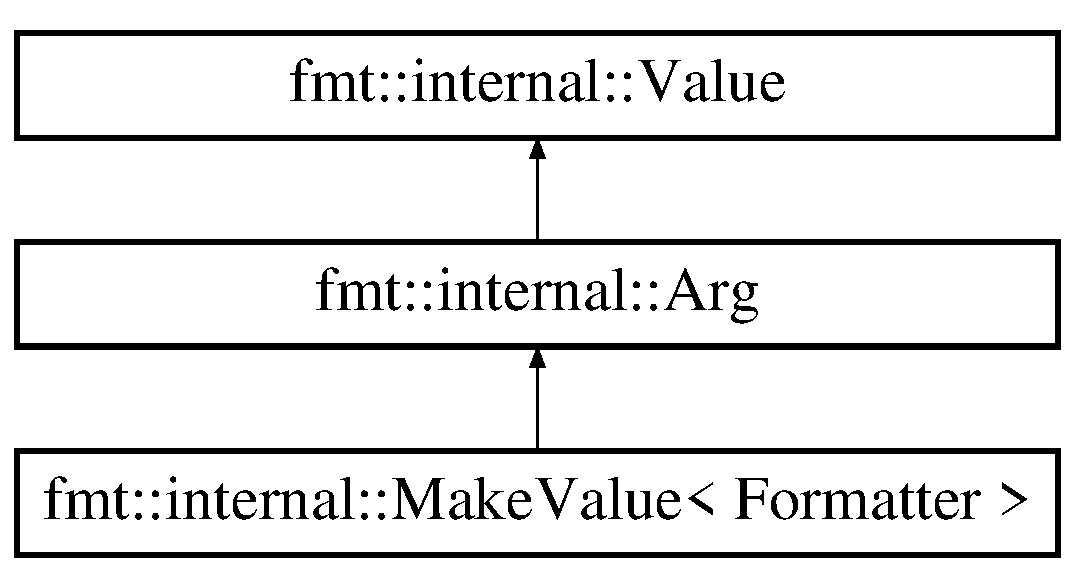
\includegraphics[height=3.000000cm]{classfmt_1_1internal_1_1MakeValue}
\end{center}
\end{figure}
\subsection*{Public Types}
\begin{DoxyCompactItemize}
\item 
typedef Formatter\+::\+Char {\bfseries Char}\hypertarget{classfmt_1_1internal_1_1MakeValue_a6c7944899a1c1ba1dd5102131d19c443}{}\label{classfmt_1_1internal_1_1MakeValue_a6c7944899a1c1ba1dd5102131d19c443}

\end{DoxyCompactItemize}
\subsection*{Public Member Functions}
\begin{DoxyCompactItemize}
\item 
{\bfseries Make\+Value} (long value)\hypertarget{classfmt_1_1internal_1_1MakeValue_ad7e52c1fc3d087a666bdd55bfda0c79c}{}\label{classfmt_1_1internal_1_1MakeValue_ad7e52c1fc3d087a666bdd55bfda0c79c}

\item 
{\bfseries Make\+Value} (unsigned long value)\hypertarget{classfmt_1_1internal_1_1MakeValue_a09061194386798ee1f7652ff0100192e}{}\label{classfmt_1_1internal_1_1MakeValue_a09061194386798ee1f7652ff0100192e}

\item 
{\bfseries Make\+Value} (typename \hyperlink{structfmt_1_1internal_1_1WCharHelper}{W\+Char\+Helper}$<$ wchar\+\_\+t, Char $>$\+::Supported value)\hypertarget{classfmt_1_1internal_1_1MakeValue_acee23248667dcf84353cecf3e8f28d67}{}\label{classfmt_1_1internal_1_1MakeValue_acee23248667dcf84353cecf3e8f28d67}

\item 
{\footnotesize template$<$typename T $>$ }\\{\bfseries Make\+Value} (const T \&value, typename \hyperlink{structfmt_1_1internal_1_1EnableIf}{Enable\+If}$<$ \hyperlink{structfmt_1_1internal_1_1Not}{Not}$<$ \hyperlink{structfmt_1_1internal_1_1ConvertToInt}{Convert\+To\+Int}$<$ T $>$\+::value $>$\+::value, int $>$\+::type=0)\hypertarget{classfmt_1_1internal_1_1MakeValue_a84e3301c4bda7c59a0d065462b4c7de5}{}\label{classfmt_1_1internal_1_1MakeValue_a84e3301c4bda7c59a0d065462b4c7de5}

\item 
{\footnotesize template$<$typename T $>$ }\\{\bfseries Make\+Value} (const T \&value, typename \hyperlink{structfmt_1_1internal_1_1EnableIf}{Enable\+If}$<$ \hyperlink{structfmt_1_1internal_1_1ConvertToInt}{Convert\+To\+Int}$<$ T $>$\+::value, int $>$\+::type=0)\hypertarget{classfmt_1_1internal_1_1MakeValue_a7635061558249117606a4facce211b03}{}\label{classfmt_1_1internal_1_1MakeValue_a7635061558249117606a4facce211b03}

\item 
{\footnotesize template$<$typename Char\+\_\+ $>$ }\\{\bfseries Make\+Value} (const \hyperlink{structfmt_1_1internal_1_1NamedArg}{Named\+Arg}$<$ Char\+\_\+ $>$ \&value)\hypertarget{classfmt_1_1internal_1_1MakeValue_a282289e2dd46a048c06d4994423e1fa4}{}\label{classfmt_1_1internal_1_1MakeValue_a282289e2dd46a048c06d4994423e1fa4}

\end{DoxyCompactItemize}
\subsection*{Static Public Member Functions}
\begin{DoxyCompactItemize}
\item 
static uint64\+\_\+t {\bfseries type} (long)\hypertarget{classfmt_1_1internal_1_1MakeValue_a595ab8ee3b95d916881ffe40db3a13b0}{}\label{classfmt_1_1internal_1_1MakeValue_a595ab8ee3b95d916881ffe40db3a13b0}

\item 
static uint64\+\_\+t {\bfseries type} (unsigned long)\hypertarget{classfmt_1_1internal_1_1MakeValue_a797f6663d8fdaf02cf254c05dbb19647}{}\label{classfmt_1_1internal_1_1MakeValue_a797f6663d8fdaf02cf254c05dbb19647}

\item 
static uint64\+\_\+t {\bfseries type} (wchar\+\_\+t)\hypertarget{classfmt_1_1internal_1_1MakeValue_adf70f5e369c149ce2916b73bea8c2af9}{}\label{classfmt_1_1internal_1_1MakeValue_adf70f5e369c149ce2916b73bea8c2af9}

\item 
{\footnotesize template$<$typename T $>$ }\\static uint64\+\_\+t {\bfseries type} (const T \&)\hypertarget{classfmt_1_1internal_1_1MakeValue_ada410611bcfef70448489daaf4b0e66a}{}\label{classfmt_1_1internal_1_1MakeValue_ada410611bcfef70448489daaf4b0e66a}

\item 
{\footnotesize template$<$typename Char\+\_\+ $>$ }\\static uint64\+\_\+t {\bfseries type} (const \hyperlink{structfmt_1_1internal_1_1NamedArg}{Named\+Arg}$<$ Char\+\_\+ $>$ \&)\hypertarget{classfmt_1_1internal_1_1MakeValue_a346c9fe85895cf679c651ec45e726a64}{}\label{classfmt_1_1internal_1_1MakeValue_a346c9fe85895cf679c651ec45e726a64}

\end{DoxyCompactItemize}
\subsection*{Additional Inherited Members}


The documentation for this class was generated from the following file\+:\begin{DoxyCompactItemize}
\item 
cvdi-\/src/cvdi-\/cl/include/spdlog/fmt/bundled/format.\+h\end{DoxyCompactItemize}

\hypertarget{classhmm__mm_1_1Mark}{}\section{hmm\+\_\+mm\+:\+:Mark Class Reference}
\label{classhmm__mm_1_1Mark}\index{hmm\+\_\+mm\+::\+Mark@{hmm\+\_\+mm\+::\+Mark}}


\hyperlink{classhmm__mm_1_1Mark}{Mark} used for routing.  




{\ttfamily \#include $<$hmm\+\_\+mm.\+hpp$>$}

\subsection*{Public Types}
\begin{DoxyCompactItemize}
\item 
using {\bfseries Ptr} = std\+::shared\+\_\+ptr$<$ \hyperlink{classhmm__mm_1_1Mark}{Mark} $>$\hypertarget{classhmm__mm_1_1Mark_a2f6ed3246a19eed051b0922c4f2cb309}{}\label{classhmm__mm_1_1Mark_a2f6ed3246a19eed051b0922c4f2cb309}

\end{DoxyCompactItemize}
\subsection*{Public Member Functions}
\begin{DoxyCompactItemize}
\item 
{\bfseries Mark} (geo\+::\+Edge\+::\+Ptr mark\+\_\+edge, geo\+::\+Edge\+::\+Ptr predecessor, double cost, double bounding\+\_\+cost)\hypertarget{classhmm__mm_1_1Mark_a5b87a7105bd09af133ee0dc7bd7615b2}{}\label{classhmm__mm_1_1Mark_a5b87a7105bd09af133ee0dc7bd7615b2}

\end{DoxyCompactItemize}
\subsection*{Public Attributes}
\begin{DoxyCompactItemize}
\item 
geo\+::\+Edge\+::\+Ptr {\bfseries mark\+\_\+edge}\hypertarget{classhmm__mm_1_1Mark_a81a92d074c7b4ff9c98cde367d0e294f}{}\label{classhmm__mm_1_1Mark_a81a92d074c7b4ff9c98cde367d0e294f}

\item 
geo\+::\+Edge\+::\+Ptr {\bfseries predecessor}\hypertarget{classhmm__mm_1_1Mark_a2a9ffe974a2508f425d8f399c66a6b68}{}\label{classhmm__mm_1_1Mark_a2a9ffe974a2508f425d8f399c66a6b68}

\item 
double {\bfseries cost}\hypertarget{classhmm__mm_1_1Mark_a127678a9257842e1478d2e17efad4860}{}\label{classhmm__mm_1_1Mark_a127678a9257842e1478d2e17efad4860}

\item 
double {\bfseries bounding\+\_\+cost}\hypertarget{classhmm__mm_1_1Mark_a9e7a0a3fe07720ecd17e698e2d6fc16f}{}\label{classhmm__mm_1_1Mark_a9e7a0a3fe07720ecd17e698e2d6fc16f}

\end{DoxyCompactItemize}


\subsection{Detailed Description}
\hyperlink{classhmm__mm_1_1Mark}{Mark} used for routing. 

The documentation for this class was generated from the following files\+:\begin{DoxyCompactItemize}
\item 
cvdi-\/src/hmm-\/mm/include/hmm\+\_\+mm.\+hpp\item 
cvdi-\/src/hmm-\/mm/src/hmm\+\_\+mm.\+cpp\end{DoxyCompactItemize}

\hypertarget{classhmm__mm_1_1MarkComparison}{}\section{hmm\+\_\+mm\+:\+:Mark\+Comparison Class Reference}
\label{classhmm__mm_1_1MarkComparison}\index{hmm\+\_\+mm\+::\+Mark\+Comparison@{hmm\+\_\+mm\+::\+Mark\+Comparison}}


Comparison \hyperlink{classhmm__mm_1_1Mark}{Mark} objects used in routing.  




{\ttfamily \#include $<$hmm\+\_\+mm.\+hpp$>$}

\subsection*{Public Member Functions}
\begin{DoxyCompactItemize}
\item 
bool {\bfseries operator()} (const Mark\+::\+Ptr \&lhs, const Mark\+::\+Ptr \&rhs) const \hypertarget{classhmm__mm_1_1MarkComparison_a249280c0776b8e8e927301aafdbfccbc}{}\label{classhmm__mm_1_1MarkComparison_a249280c0776b8e8e927301aafdbfccbc}

\end{DoxyCompactItemize}


\subsection{Detailed Description}
Comparison \hyperlink{classhmm__mm_1_1Mark}{Mark} objects used in routing. 

The documentation for this class was generated from the following file\+:\begin{DoxyCompactItemize}
\item 
cvdi-\/src/hmm-\/mm/include/hmm\+\_\+mm.\+hpp\end{DoxyCompactItemize}

\hypertarget{classhmm__mm_1_1Matcher}{}\section{hmm\+\_\+mm\+:\+:Matcher Class Reference}
\label{classhmm__mm_1_1Matcher}\index{hmm\+\_\+mm\+::\+Matcher@{hmm\+\_\+mm\+::\+Matcher}}


Hidden Markov Model Map \hyperlink{classhmm__mm_1_1Matcher}{Matcher} for sequential G\+PS traces.  




{\ttfamily \#include $<$hmm\+\_\+mm.\+hpp$>$}

\subsection*{Public Member Functions}
\begin{DoxyCompactItemize}
\item 
\hyperlink{classhmm__mm_1_1Matcher_a4a1a9eafcddc6c98789e056121f55ee1}{Matcher} (double min\+\_\+distance, long min\+\_\+time, int k=-\/1, long t=-\/1)
\begin{DoxyCompactList}\small\item\em Construct a \hyperlink{classhmm__mm_1_1Matcher}{Matcher} object. \end{DoxyCompactList}\item 
void \hyperlink{classhmm__mm_1_1Matcher_ab6ead19f86c9ed2711d0b6e4cc20365a}{map\+\_\+match} (\hyperlink{classhmm__mm_1_1RoadMap}{Road\+Map} \&road\+\_\+map, geo\+\_\+data\+::\+Sample\+::\+Trace \&trace)
\begin{DoxyCompactList}\small\item\em Map match samples in a sequential G\+PS trace. Sets the matched edge for each \hyperlink{classgeo__data_1_1Sample}{geo\+\_\+data\+::\+Sample} object until the end of trace is reached, or a break in the Hidden Markov Model occurs. \end{DoxyCompactList}\end{DoxyCompactItemize}


\subsection{Detailed Description}
Hidden Markov Model Map \hyperlink{classhmm__mm_1_1Matcher}{Matcher} for sequential G\+PS traces. 

\subsection{Constructor \& Destructor Documentation}
\index{hmm\+\_\+mm\+::\+Matcher@{hmm\+\_\+mm\+::\+Matcher}!Matcher@{Matcher}}
\index{Matcher@{Matcher}!hmm\+\_\+mm\+::\+Matcher@{hmm\+\_\+mm\+::\+Matcher}}
\subsubsection[{\texorpdfstring{Matcher(double min\+\_\+distance, long min\+\_\+time, int k=-\/1, long t=-\/1)}{Matcher(double min_distance, long min_time, int k=-1, long t=-1)}}]{\setlength{\rightskip}{0pt plus 5cm}hmm\+\_\+mm\+::\+Matcher\+::\+Matcher (
\begin{DoxyParamCaption}
\item[{double}]{min\+\_\+distance, }
\item[{long}]{min\+\_\+time, }
\item[{int}]{k = {\ttfamily -\/1}, }
\item[{long}]{t = {\ttfamily -\/1}}
\end{DoxyParamCaption}
)}\hypertarget{classhmm__mm_1_1Matcher_a4a1a9eafcddc6c98789e056121f55ee1}{}\label{classhmm__mm_1_1Matcher_a4a1a9eafcddc6c98789e056121f55ee1}


Construct a \hyperlink{classhmm__mm_1_1Matcher}{Matcher} object. 


\begin{DoxyParams}{Parameters}
{\em min\+\_\+distance} & minimum distance, in meters, between samples in the model \\
\hline
{\em min\+\_\+time} & minimum time, in seconds, between samples in the model \\
\hline
{\em k} & not used \\
\hline
{\em t} & not used \\
\hline
\end{DoxyParams}


\subsection{Member Function Documentation}
\index{hmm\+\_\+mm\+::\+Matcher@{hmm\+\_\+mm\+::\+Matcher}!map\+\_\+match@{map\+\_\+match}}
\index{map\+\_\+match@{map\+\_\+match}!hmm\+\_\+mm\+::\+Matcher@{hmm\+\_\+mm\+::\+Matcher}}
\subsubsection[{\texorpdfstring{map\+\_\+match(\+Road\+Map \&road\+\_\+map, geo\+\_\+data\+::\+Sample\+::\+Trace \&trace)}{map_match(RoadMap &road_map, geo_data::Sample::Trace &trace)}}]{\setlength{\rightskip}{0pt plus 5cm}void hmm\+\_\+mm\+::\+Matcher\+::map\+\_\+match (
\begin{DoxyParamCaption}
\item[{{\bf Road\+Map} \&}]{road\+\_\+map, }
\item[{geo\+\_\+data\+::\+Sample\+::\+Trace \&}]{trace}
\end{DoxyParamCaption}
)}\hypertarget{classhmm__mm_1_1Matcher_ab6ead19f86c9ed2711d0b6e4cc20365a}{}\label{classhmm__mm_1_1Matcher_ab6ead19f86c9ed2711d0b6e4cc20365a}


Map match samples in a sequential G\+PS trace. Sets the matched edge for each \hyperlink{classgeo__data_1_1Sample}{geo\+\_\+data\+::\+Sample} object until the end of trace is reached, or a break in the Hidden Markov Model occurs. 


\begin{DoxyParams}{Parameters}
{\em road\+\_\+map} & the geo\+\_\+data\+::\+Road\+Map object to used for candidates and transitions. \\
\hline
{\em trace} & the sample G\+PS trace \\
\hline
\end{DoxyParams}


The documentation for this class was generated from the following files\+:\begin{DoxyCompactItemize}
\item 
cvdi-\/src/hmm-\/mm/include/hmm\+\_\+mm.\+hpp\item 
cvdi-\/src/hmm-\/mm/src/hmm\+\_\+mm.\+cpp\end{DoxyCompactItemize}

\hypertarget{classfmt_1_1internal_1_1MemoryBuffer}{}\section{fmt\+:\+:internal\+:\+:Memory\+Buffer$<$ T, S\+I\+ZE, Allocator $>$ Class Template Reference}
\label{classfmt_1_1internal_1_1MemoryBuffer}\index{fmt\+::internal\+::\+Memory\+Buffer$<$ T, S\+I\+Z\+E, Allocator $>$@{fmt\+::internal\+::\+Memory\+Buffer$<$ T, S\+I\+Z\+E, Allocator $>$}}
Inheritance diagram for fmt\+:\+:internal\+:\+:Memory\+Buffer$<$ T, S\+I\+ZE, Allocator $>$\+:\begin{figure}[H]
\begin{center}
\leavevmode
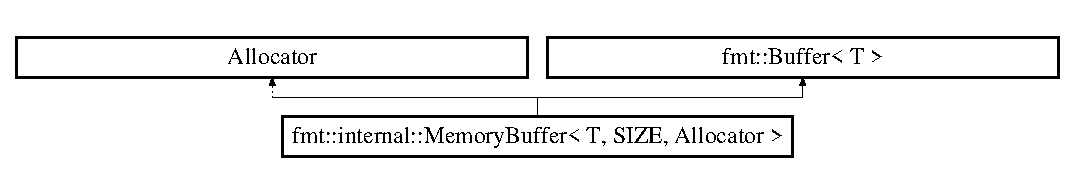
\includegraphics[height=1.872910cm]{classfmt_1_1internal_1_1MemoryBuffer}
\end{center}
\end{figure}
\subsection*{Public Member Functions}
\begin{DoxyCompactItemize}
\item 
{\bfseries Memory\+Buffer} (const Allocator \&alloc=Allocator())\hypertarget{classfmt_1_1internal_1_1MemoryBuffer_af3325b8e955a9c84a51c31570bcab893}{}\label{classfmt_1_1internal_1_1MemoryBuffer_af3325b8e955a9c84a51c31570bcab893}

\item 
Allocator {\bfseries get\+\_\+allocator} () const \hypertarget{classfmt_1_1internal_1_1MemoryBuffer_a6cf259337ce910f8864512d664daf66f}{}\label{classfmt_1_1internal_1_1MemoryBuffer_a6cf259337ce910f8864512d664daf66f}

\end{DoxyCompactItemize}
\subsection*{Protected Member Functions}
\begin{DoxyCompactItemize}
\item 
void \hyperlink{classfmt_1_1internal_1_1MemoryBuffer_a6ecee679d5caf3345f8ffae92b7ca702}{grow} (std\+::size\+\_\+t \hyperlink{classfmt_1_1Buffer_a14fa72f0ddf584c14ffffb1446f598aa}{size}) F\+M\+T\+\_\+\+O\+V\+E\+R\+R\+I\+DE
\end{DoxyCompactItemize}
\subsection*{Additional Inherited Members}


\subsection{Member Function Documentation}
\index{fmt\+::internal\+::\+Memory\+Buffer@{fmt\+::internal\+::\+Memory\+Buffer}!grow@{grow}}
\index{grow@{grow}!fmt\+::internal\+::\+Memory\+Buffer@{fmt\+::internal\+::\+Memory\+Buffer}}
\subsubsection[{\texorpdfstring{grow(std\+::size\+\_\+t size) F\+M\+T\+\_\+\+O\+V\+E\+R\+R\+I\+DE}{grow(std::size_t size) FMT_OVERRIDE}}]{\setlength{\rightskip}{0pt plus 5cm}template$<$typename T , std\+::size\+\_\+t S\+I\+ZE, typename Allocator $>$ void {\bf fmt\+::internal\+::\+Memory\+Buffer}$<$ T, S\+I\+ZE, Allocator $>$\+::grow (
\begin{DoxyParamCaption}
\item[{std\+::size\+\_\+t}]{size}
\end{DoxyParamCaption}
)\hspace{0.3cm}{\ttfamily [protected]}, {\ttfamily [virtual]}}\hypertarget{classfmt_1_1internal_1_1MemoryBuffer_a6ecee679d5caf3345f8ffae92b7ca702}{}\label{classfmt_1_1internal_1_1MemoryBuffer_a6ecee679d5caf3345f8ffae92b7ca702}
Increases the buffer capacity to hold at least {\itshape size} elements updating {\ttfamily ptr\+\_\+} and {\ttfamily capacity\+\_\+}.  

Implements \hyperlink{classfmt_1_1Buffer_abdc7aaf5813aa07008b3d715969a7e19}{fmt\+::\+Buffer$<$ T $>$}.



The documentation for this class was generated from the following file\+:\begin{DoxyCompactItemize}
\item 
cvdi-\/src/cvdi-\/cl/include/spdlog/fmt/bundled/format.\+h\end{DoxyCompactItemize}

\hypertarget{classspdlog_1_1details_1_1mpmc__bounded__queue}{}\section{spdlog\+:\+:details\+:\+:mpmc\+\_\+bounded\+\_\+queue$<$ T $>$ Class Template Reference}
\label{classspdlog_1_1details_1_1mpmc__bounded__queue}\index{spdlog\+::details\+::mpmc\+\_\+bounded\+\_\+queue$<$ T $>$@{spdlog\+::details\+::mpmc\+\_\+bounded\+\_\+queue$<$ T $>$}}
\subsection*{Public Types}
\begin{DoxyCompactItemize}
\item 
using {\bfseries item\+\_\+type} = T\hypertarget{classspdlog_1_1details_1_1mpmc__bounded__queue_a031988ff55da961ad0cd1df08c9112b5}{}\label{classspdlog_1_1details_1_1mpmc__bounded__queue_a031988ff55da961ad0cd1df08c9112b5}

\end{DoxyCompactItemize}
\subsection*{Public Member Functions}
\begin{DoxyCompactItemize}
\item 
{\bfseries mpmc\+\_\+bounded\+\_\+queue} (size\+\_\+t buffer\+\_\+size)\hypertarget{classspdlog_1_1details_1_1mpmc__bounded__queue_ab624df4f131d8b943bf8c451e643ddcb}{}\label{classspdlog_1_1details_1_1mpmc__bounded__queue_ab624df4f131d8b943bf8c451e643ddcb}

\item 
bool {\bfseries enqueue} (T \&\&data)\hypertarget{classspdlog_1_1details_1_1mpmc__bounded__queue_a61b70c6eee62cea308127373bdc9deee}{}\label{classspdlog_1_1details_1_1mpmc__bounded__queue_a61b70c6eee62cea308127373bdc9deee}

\item 
bool {\bfseries dequeue} (T \&data)\hypertarget{classspdlog_1_1details_1_1mpmc__bounded__queue_a97ff1f28e98db6c55970843d6193c047}{}\label{classspdlog_1_1details_1_1mpmc__bounded__queue_a97ff1f28e98db6c55970843d6193c047}

\item 
size\+\_\+t {\bfseries approx\+\_\+size} ()\hypertarget{classspdlog_1_1details_1_1mpmc__bounded__queue_ab9c60fc728432e81d18a07cccc8d4ad7}{}\label{classspdlog_1_1details_1_1mpmc__bounded__queue_ab9c60fc728432e81d18a07cccc8d4ad7}

\end{DoxyCompactItemize}


The documentation for this class was generated from the following file\+:\begin{DoxyCompactItemize}
\item 
cvdi-\/src/cvdi-\/cl/include/spdlog/details/mpmc\+\_\+bounded\+\_\+q.\+h\end{DoxyCompactItemize}

\hypertarget{structfmt_1_1internal_1_1NamedArg}{}\section{fmt\+:\+:internal\+:\+:Named\+Arg$<$ Char $>$ Struct Template Reference}
\label{structfmt_1_1internal_1_1NamedArg}\index{fmt\+::internal\+::\+Named\+Arg$<$ Char $>$@{fmt\+::internal\+::\+Named\+Arg$<$ Char $>$}}
Inheritance diagram for fmt\+:\+:internal\+:\+:Named\+Arg$<$ Char $>$\+:\begin{figure}[H]
\begin{center}
\leavevmode
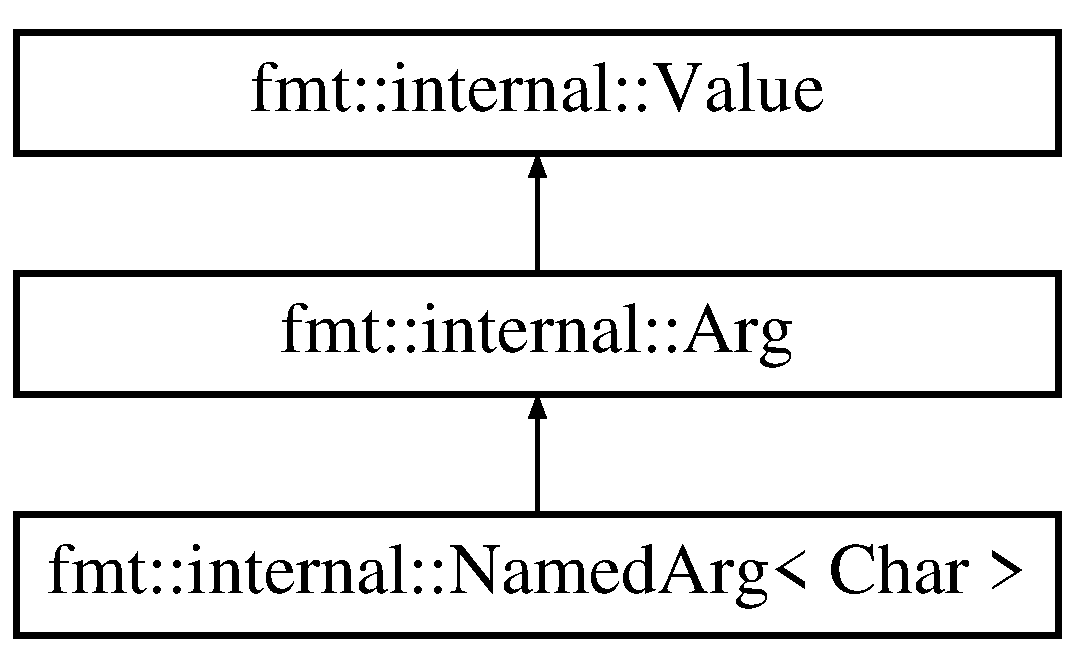
\includegraphics[height=3.000000cm]{structfmt_1_1internal_1_1NamedArg}
\end{center}
\end{figure}
\subsection*{Public Member Functions}
\begin{DoxyCompactItemize}
\item 
{\footnotesize template$<$typename T $>$ }\\{\bfseries Named\+Arg} (\hyperlink{classfmt_1_1BasicStringRef}{Basic\+String\+Ref}$<$ Char $>$ argname, const T \&value)\hypertarget{structfmt_1_1internal_1_1NamedArg_a44557d139403597d7e4c73013f98db73}{}\label{structfmt_1_1internal_1_1NamedArg_a44557d139403597d7e4c73013f98db73}

\end{DoxyCompactItemize}
\subsection*{Public Attributes}
\begin{DoxyCompactItemize}
\item 
\hyperlink{classfmt_1_1BasicStringRef}{Basic\+String\+Ref}$<$ Char $>$ {\bfseries name}\hypertarget{structfmt_1_1internal_1_1NamedArg_ab2e3ffba4fa9df8122ed586134eac2c9}{}\label{structfmt_1_1internal_1_1NamedArg_ab2e3ffba4fa9df8122ed586134eac2c9}

\end{DoxyCompactItemize}
\subsection*{Additional Inherited Members}


The documentation for this struct was generated from the following file\+:\begin{DoxyCompactItemize}
\item 
cvdi-\/src/cvdi-\/cl/include/spdlog/fmt/bundled/format.\+h\end{DoxyCompactItemize}

\hypertarget{structfmt_1_1internal_1_1Not}{}\section{fmt\+:\+:internal\+:\+:Not$<$ bool $>$ Struct Template Reference}
\label{structfmt_1_1internal_1_1Not}\index{fmt\+::internal\+::\+Not$<$ bool $>$@{fmt\+::internal\+::\+Not$<$ bool $>$}}
\subsection*{Public Types}
\begin{DoxyCompactItemize}
\item 
enum \{ {\bfseries value} = 0
 \}\hypertarget{structfmt_1_1internal_1_1Not_a878274638da25a62562a1d52b4053bf0}{}\label{structfmt_1_1internal_1_1Not_a878274638da25a62562a1d52b4053bf0}

\end{DoxyCompactItemize}


The documentation for this struct was generated from the following file\+:\begin{DoxyCompactItemize}
\item 
cvdi-\/src/cvdi-\/cl/include/spdlog/fmt/bundled/format.\+h\end{DoxyCompactItemize}

\hypertarget{structfmt_1_1internal_1_1Not_3_01false_01_4}{}\section{fmt\+:\+:internal\+:\+:Not$<$ false $>$ Struct Template Reference}
\label{structfmt_1_1internal_1_1Not_3_01false_01_4}\index{fmt\+::internal\+::\+Not$<$ false $>$@{fmt\+::internal\+::\+Not$<$ false $>$}}
\subsection*{Public Types}
\begin{DoxyCompactItemize}
\item 
enum \{ {\bfseries value} = 1
 \}\hypertarget{structfmt_1_1internal_1_1Not_3_01false_01_4_a2ec5a6c33abbed29c45dba33cca3c4f8}{}\label{structfmt_1_1internal_1_1Not_3_01false_01_4_a2ec5a6c33abbed29c45dba33cca3c4f8}

\end{DoxyCompactItemize}


The documentation for this struct was generated from the following file\+:\begin{DoxyCompactItemize}
\item 
cvdi-\/src/cvdi-\/cl/include/spdlog/fmt/bundled/format.\+h\end{DoxyCompactItemize}

\hypertarget{structfmt_1_1internal_1_1NoThousandsSep}{}\section{fmt\+:\+:internal\+:\+:No\+Thousands\+Sep Struct Reference}
\label{structfmt_1_1internal_1_1NoThousandsSep}\index{fmt\+::internal\+::\+No\+Thousands\+Sep@{fmt\+::internal\+::\+No\+Thousands\+Sep}}
\subsection*{Public Member Functions}
\begin{DoxyCompactItemize}
\item 
{\footnotesize template$<$typename Char $>$ }\\void {\bfseries operator()} (Char $\ast$)\hypertarget{structfmt_1_1internal_1_1NoThousandsSep_ab253f8385a85334b2fd9b0bfb551a6a6}{}\label{structfmt_1_1internal_1_1NoThousandsSep_ab253f8385a85334b2fd9b0bfb551a6a6}

\end{DoxyCompactItemize}


The documentation for this struct was generated from the following file\+:\begin{DoxyCompactItemize}
\item 
cvdi-\/src/cvdi-\/cl/include/spdlog/fmt/bundled/format.\+h\end{DoxyCompactItemize}

\hypertarget{structfmt_1_1internal_1_1Null}{}\section{fmt\+:\+:internal\+:\+:Null$<$ T $>$ Struct Template Reference}
\label{structfmt_1_1internal_1_1Null}\index{fmt\+::internal\+::\+Null$<$ T $>$@{fmt\+::internal\+::\+Null$<$ T $>$}}


The documentation for this struct was generated from the following file\+:\begin{DoxyCompactItemize}
\item 
cvdi-\/src/cvdi-\/cl/include/spdlog/fmt/bundled/format.\+h\end{DoxyCompactItemize}

\hypertarget{structspdlog_1_1details_1_1null__atomic__int}{}\section{spdlog\+:\+:details\+:\+:null\+\_\+atomic\+\_\+int Struct Reference}
\label{structspdlog_1_1details_1_1null__atomic__int}\index{spdlog\+::details\+::null\+\_\+atomic\+\_\+int@{spdlog\+::details\+::null\+\_\+atomic\+\_\+int}}
\subsection*{Public Member Functions}
\begin{DoxyCompactItemize}
\item 
{\bfseries null\+\_\+atomic\+\_\+int} (int val)\hypertarget{structspdlog_1_1details_1_1null__atomic__int_aa9856518fa8bc88f466b2b9c17bff1b9}{}\label{structspdlog_1_1details_1_1null__atomic__int_aa9856518fa8bc88f466b2b9c17bff1b9}

\item 
int {\bfseries load} (std\+::memory\+\_\+order) const \hypertarget{structspdlog_1_1details_1_1null__atomic__int_a9ddf324260ae269cf124e6158a6a4188}{}\label{structspdlog_1_1details_1_1null__atomic__int_a9ddf324260ae269cf124e6158a6a4188}

\item 
void {\bfseries store} (int val)\hypertarget{structspdlog_1_1details_1_1null__atomic__int_a75c74956220ca5cc82a4eedcd9aa854f}{}\label{structspdlog_1_1details_1_1null__atomic__int_a75c74956220ca5cc82a4eedcd9aa854f}

\end{DoxyCompactItemize}
\subsection*{Public Attributes}
\begin{DoxyCompactItemize}
\item 
int {\bfseries value}\hypertarget{structspdlog_1_1details_1_1null__atomic__int_ab433069a53cdd1402dc7b0b942d7095f}{}\label{structspdlog_1_1details_1_1null__atomic__int_ab433069a53cdd1402dc7b0b942d7095f}

\end{DoxyCompactItemize}


The documentation for this struct was generated from the following file\+:\begin{DoxyCompactItemize}
\item 
cvdi-\/src/cvdi-\/cl/include/spdlog/details/null\+\_\+mutex.\+h\end{DoxyCompactItemize}

\hypertarget{structspdlog_1_1details_1_1null__mutex}{}\section{spdlog\+:\+:details\+:\+:null\+\_\+mutex Struct Reference}
\label{structspdlog_1_1details_1_1null__mutex}\index{spdlog\+::details\+::null\+\_\+mutex@{spdlog\+::details\+::null\+\_\+mutex}}
\subsection*{Public Member Functions}
\begin{DoxyCompactItemize}
\item 
void {\bfseries lock} ()\hypertarget{structspdlog_1_1details_1_1null__mutex_acaccd5741a4d60756a2c23018f670b9a}{}\label{structspdlog_1_1details_1_1null__mutex_acaccd5741a4d60756a2c23018f670b9a}

\item 
void {\bfseries unlock} ()\hypertarget{structspdlog_1_1details_1_1null__mutex_acbc27862ec43b4b0e9c8f5197174f95f}{}\label{structspdlog_1_1details_1_1null__mutex_acbc27862ec43b4b0e9c8f5197174f95f}

\item 
bool {\bfseries try\+\_\+lock} ()\hypertarget{structspdlog_1_1details_1_1null__mutex_a1e367b1adaa6305edbe163c4d2021c53}{}\label{structspdlog_1_1details_1_1null__mutex_a1e367b1adaa6305edbe163c4d2021c53}

\end{DoxyCompactItemize}


The documentation for this struct was generated from the following file\+:\begin{DoxyCompactItemize}
\item 
cvdi-\/src/cvdi-\/cl/include/spdlog/details/null\+\_\+mutex.\+h\end{DoxyCompactItemize}

\hypertarget{classspdlog_1_1sinks_1_1null__sink}{}\section{spdlog\+:\+:sinks\+:\+:null\+\_\+sink$<$ Mutex $>$ Class Template Reference}
\label{classspdlog_1_1sinks_1_1null__sink}\index{spdlog\+::sinks\+::null\+\_\+sink$<$ Mutex $>$@{spdlog\+::sinks\+::null\+\_\+sink$<$ Mutex $>$}}
Inheritance diagram for spdlog\+:\+:sinks\+:\+:null\+\_\+sink$<$ Mutex $>$\+:\begin{figure}[H]
\begin{center}
\leavevmode
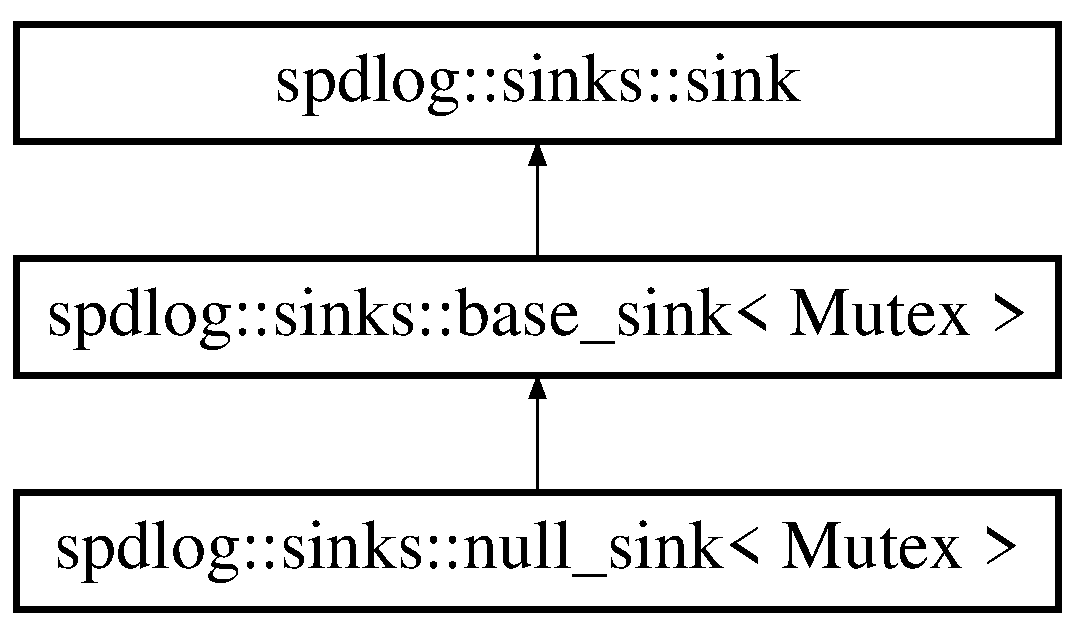
\includegraphics[height=3.000000cm]{classspdlog_1_1sinks_1_1null__sink}
\end{center}
\end{figure}
\subsection*{Protected Member Functions}
\begin{DoxyCompactItemize}
\item 
void {\bfseries \+\_\+sink\+\_\+it} (const \hyperlink{structspdlog_1_1details_1_1log__msg}{details\+::log\+\_\+msg} \&) override\hypertarget{classspdlog_1_1sinks_1_1null__sink_aa3d6b00b230165fd17c6823665c1c289}{}\label{classspdlog_1_1sinks_1_1null__sink_aa3d6b00b230165fd17c6823665c1c289}

\item 
void {\bfseries \+\_\+flush} () override\hypertarget{classspdlog_1_1sinks_1_1null__sink_af055b5f06592bafa358fb1f7b5830229}{}\label{classspdlog_1_1sinks_1_1null__sink_af055b5f06592bafa358fb1f7b5830229}

\end{DoxyCompactItemize}
\subsection*{Additional Inherited Members}


The documentation for this class was generated from the following file\+:\begin{DoxyCompactItemize}
\item 
cvdi-\/src/cvdi-\/cl/include/spdlog/sinks/null\+\_\+sink.\+h\end{DoxyCompactItemize}

\hypertarget{classstd_1_1numeric__limits_3_01fmt_1_1internal_1_1DummyInt_01_4}{}\section{std\+:\+:numeric\+\_\+limits$<$ fmt\+:\+:internal\+:\+:Dummy\+Int $>$ Class Template Reference}
\label{classstd_1_1numeric__limits_3_01fmt_1_1internal_1_1DummyInt_01_4}\index{std\+::numeric\+\_\+limits$<$ fmt\+::internal\+::\+Dummy\+Int $>$@{std\+::numeric\+\_\+limits$<$ fmt\+::internal\+::\+Dummy\+Int $>$}}
Inheritance diagram for std\+:\+:numeric\+\_\+limits$<$ fmt\+:\+:internal\+:\+:Dummy\+Int $>$\+:\begin{figure}[H]
\begin{center}
\leavevmode
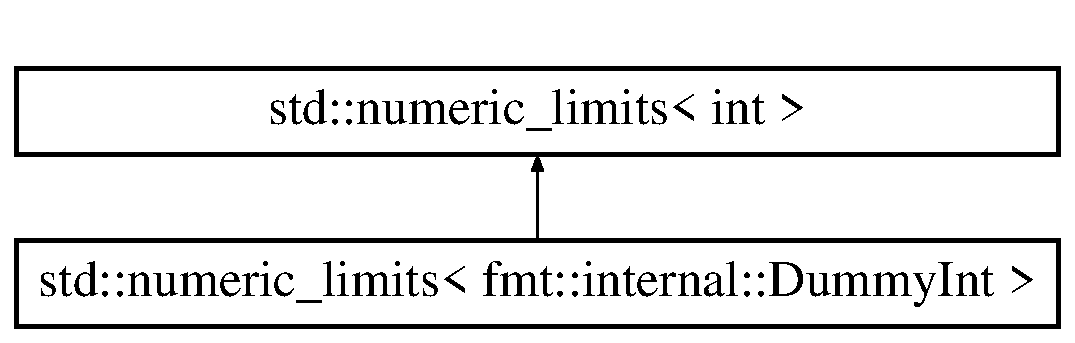
\includegraphics[height=2.000000cm]{classstd_1_1numeric__limits_3_01fmt_1_1internal_1_1DummyInt_01_4}
\end{center}
\end{figure}
\subsection*{Static Public Member Functions}
\begin{DoxyCompactItemize}
\item 
{\footnotesize template$<$typename T $>$ }\\static bool {\bfseries isinfinity} (T x)\hypertarget{classstd_1_1numeric__limits_3_01fmt_1_1internal_1_1DummyInt_01_4_abd1469673d6c36a014a988bce1dfb0ee}{}\label{classstd_1_1numeric__limits_3_01fmt_1_1internal_1_1DummyInt_01_4_abd1469673d6c36a014a988bce1dfb0ee}

\item 
{\footnotesize template$<$typename T $>$ }\\static bool {\bfseries isnotanumber} (T x)\hypertarget{classstd_1_1numeric__limits_3_01fmt_1_1internal_1_1DummyInt_01_4_a89433356fbf5b68eb0c13208a5e3b6b1}{}\label{classstd_1_1numeric__limits_3_01fmt_1_1internal_1_1DummyInt_01_4_a89433356fbf5b68eb0c13208a5e3b6b1}

\item 
static bool {\bfseries isnegative} (double x)\hypertarget{classstd_1_1numeric__limits_3_01fmt_1_1internal_1_1DummyInt_01_4_a1cc82945f63918e9a8603d3ef750990d}{}\label{classstd_1_1numeric__limits_3_01fmt_1_1internal_1_1DummyInt_01_4_a1cc82945f63918e9a8603d3ef750990d}

\end{DoxyCompactItemize}


The documentation for this class was generated from the following file\+:\begin{DoxyCompactItemize}
\item 
cvdi-\/src/cvdi-\/cl/include/spdlog/fmt/bundled/format.\+h\end{DoxyCompactItemize}

\hypertarget{classtool_1_1Option}{}\section{tool\+:\+:Option Class Reference}
\label{classtool_1_1Option}\index{tool\+::\+Option@{tool\+::\+Option}}


A basic command line option.  




{\ttfamily \#include $<$tool.\+hpp$>$}

\subsection*{Public Member Functions}
\begin{DoxyCompactItemize}
\item 
\hyperlink{classtool_1_1Option_ac9f2b30a192af0e158832b0bdef9aa93}{Option} (char short\+\_\+name, const std\+::string \&long\+\_\+name, const std\+::string \&description)
\begin{DoxyCompactList}\small\item\em \hyperlink{classtool_1_1Option}{Option} constructor with no default value. \end{DoxyCompactList}\item 
\hyperlink{classtool_1_1Option_aa5467959f13a00f8a560e735b4cfde72}{Option} (char short\+\_\+name, const std\+::string \&long\+\_\+name, const std\+::string \&description, const std\+::string \&default\+\_\+val)
\begin{DoxyCompactList}\small\item\em \hyperlink{classtool_1_1Option}{Option} constructor with a default value. \end{DoxyCompactList}\item 
char \hyperlink{classtool_1_1Option_a2a50ad5b1599988a26375e0a1c26258c}{Get\+Short\+Name} (void) const 
\begin{DoxyCompactList}\small\item\em Get short name of this option. \end{DoxyCompactList}\item 
const std\+::string \& \hyperlink{classtool_1_1Option_a79fef07bc337c275e41573572b615d29}{Get\+Long\+Name} (void) const 
\begin{DoxyCompactList}\small\item\em Get the long name of this option. \end{DoxyCompactList}\item 
void \hyperlink{classtool_1_1Option_a55095d2ae73bf936c2cb944e440b84b1}{Set\+Val} (const std\+::string \&val)
\begin{DoxyCompactList}\small\item\em Set the value of this option. \end{DoxyCompactList}\item 
void \hyperlink{classtool_1_1Option_a4fec21690e82f26e9d875dc1267bc3c3}{Set\+Val} ()\hypertarget{classtool_1_1Option_a4fec21690e82f26e9d875dc1267bc3c3}{}\label{classtool_1_1Option_a4fec21690e82f26e9d875dc1267bc3c3}

\begin{DoxyCompactList}\small\item\em Set the value of this option to true. \end{DoxyCompactList}\item 
const std\+::string \& \hyperlink{classtool_1_1Option_a4d06e37da415d410a18e3facbb30abc3}{Get\+String\+Val} () const 
\begin{DoxyCompactList}\small\item\em Get the value of this option. \end{DoxyCompactList}\item 
int \hyperlink{classtool_1_1Option_a46701faf98e40b5f6a81fe0c86865b15}{Get\+Int\+Val} () const 
\begin{DoxyCompactList}\small\item\em Get the value of this option as an integer. \end{DoxyCompactList}\item 
uint64\+\_\+t \hyperlink{classtool_1_1Option_aeffb50df47db2627a232e8c04b0aeca3}{Get\+Uint64\+Val} () const 
\begin{DoxyCompactList}\small\item\em Get the value of this option as an unsigned long long (unsigned 64-\/bit). \end{DoxyCompactList}\item 
double \hyperlink{classtool_1_1Option_a2c259934e9cd770dfad1efb70a71c1f0}{Get\+Double\+Val} () const 
\begin{DoxyCompactList}\small\item\em Get the value of this option as a double. \end{DoxyCompactList}\item 
bool \hyperlink{classtool_1_1Option_ab7d08f16def63f9015d62dbfe06e628e}{Get\+Bool\+Val} () const 
\begin{DoxyCompactList}\small\item\em Get the value of this option as a boolean. This returns True if the underlying string value is anything other than an empty string. Otherwise returns False. \end{DoxyCompactList}\item 
bool \hyperlink{classtool_1_1Option_aceef342485d7f2b6c1308d7b04b1b1ea}{Is\+Flag} () const 
\begin{DoxyCompactList}\small\item\em Get the flag status of this option. \end{DoxyCompactList}\item 
bool \hyperlink{classtool_1_1Option_aac9058af5de2dd1c1d73367e1430c9e9}{Has\+Val} () const 
\begin{DoxyCompactList}\small\item\em Get the value status of this option. \end{DoxyCompactList}\end{DoxyCompactItemize}
\subsection*{Friends}
\begin{DoxyCompactItemize}
\item 
std\+::ostream \& \hyperlink{classtool_1_1Option_a8e9bf3e5994c33fa14638743683e959d}{operator$<$$<$} (std\+::ostream \&os, const \hyperlink{classtool_1_1Option}{Option} \&option)
\begin{DoxyCompactList}\small\item\em Write an \hyperlink{classtool_1_1Option}{Option} to a stream formatted for command line help output. \end{DoxyCompactList}\end{DoxyCompactItemize}


\subsection{Detailed Description}
A basic command line option. 

\subsection{Constructor \& Destructor Documentation}
\index{tool\+::\+Option@{tool\+::\+Option}!Option@{Option}}
\index{Option@{Option}!tool\+::\+Option@{tool\+::\+Option}}
\subsubsection[{\texorpdfstring{Option(char short\+\_\+name, const std\+::string \&long\+\_\+name, const std\+::string \&description)}{Option(char short_name, const std::string &long_name, const std::string &description)}}]{\setlength{\rightskip}{0pt plus 5cm}tool\+::\+Option\+::\+Option (
\begin{DoxyParamCaption}
\item[{char}]{short\+\_\+name, }
\item[{const std\+::string \&}]{long\+\_\+name, }
\item[{const std\+::string \&}]{description}
\end{DoxyParamCaption}
)}\hypertarget{classtool_1_1Option_ac9f2b30a192af0e158832b0bdef9aa93}{}\label{classtool_1_1Option_ac9f2b30a192af0e158832b0bdef9aa93}


\hyperlink{classtool_1_1Option}{Option} constructor with no default value. 


\begin{DoxyParams}{Parameters}
{\em short\+\_\+name} & the character used for the short name of the option \\
\hline
{\em long\+\_\+name} & the string used for the long name of the option \\
\hline
{\em description} & the string used for the description of the option \\
\hline
\end{DoxyParams}
\index{tool\+::\+Option@{tool\+::\+Option}!Option@{Option}}
\index{Option@{Option}!tool\+::\+Option@{tool\+::\+Option}}
\subsubsection[{\texorpdfstring{Option(char short\+\_\+name, const std\+::string \&long\+\_\+name, const std\+::string \&description, const std\+::string \&default\+\_\+val)}{Option(char short_name, const std::string &long_name, const std::string &description, const std::string &default_val)}}]{\setlength{\rightskip}{0pt plus 5cm}tool\+::\+Option\+::\+Option (
\begin{DoxyParamCaption}
\item[{char}]{short\+\_\+name, }
\item[{const std\+::string \&}]{long\+\_\+name, }
\item[{const std\+::string \&}]{description, }
\item[{const std\+::string \&}]{default\+\_\+val}
\end{DoxyParamCaption}
)}\hypertarget{classtool_1_1Option_aa5467959f13a00f8a560e735b4cfde72}{}\label{classtool_1_1Option_aa5467959f13a00f8a560e735b4cfde72}


\hyperlink{classtool_1_1Option}{Option} constructor with a default value. 


\begin{DoxyParams}{Parameters}
{\em short\+\_\+name} & the character used for the short name of the option \\
\hline
{\em long\+\_\+name} & the string used for the long name of the option \\
\hline
{\em description} & the string used for the description of the option \\
\hline
{\em default\+\_\+val} & the string used for the default value of the option \\
\hline
\end{DoxyParams}


\subsection{Member Function Documentation}
\index{tool\+::\+Option@{tool\+::\+Option}!Get\+Bool\+Val@{Get\+Bool\+Val}}
\index{Get\+Bool\+Val@{Get\+Bool\+Val}!tool\+::\+Option@{tool\+::\+Option}}
\subsubsection[{\texorpdfstring{Get\+Bool\+Val() const }{GetBoolVal() const }}]{\setlength{\rightskip}{0pt plus 5cm}bool tool\+::\+Option\+::\+Get\+Bool\+Val (
\begin{DoxyParamCaption}
{}
\end{DoxyParamCaption}
) const}\hypertarget{classtool_1_1Option_ab7d08f16def63f9015d62dbfe06e628e}{}\label{classtool_1_1Option_ab7d08f16def63f9015d62dbfe06e628e}


Get the value of this option as a boolean. This returns True if the underlying string value is anything other than an empty string. Otherwise returns False. 

\begin{DoxyReturn}{Returns}
the boolean value of this option 
\end{DoxyReturn}
\index{tool\+::\+Option@{tool\+::\+Option}!Get\+Double\+Val@{Get\+Double\+Val}}
\index{Get\+Double\+Val@{Get\+Double\+Val}!tool\+::\+Option@{tool\+::\+Option}}
\subsubsection[{\texorpdfstring{Get\+Double\+Val() const }{GetDoubleVal() const }}]{\setlength{\rightskip}{0pt plus 5cm}double tool\+::\+Option\+::\+Get\+Double\+Val (
\begin{DoxyParamCaption}
{}
\end{DoxyParamCaption}
) const}\hypertarget{classtool_1_1Option_a2c259934e9cd770dfad1efb70a71c1f0}{}\label{classtool_1_1Option_a2c259934e9cd770dfad1efb70a71c1f0}


Get the value of this option as a double. 

\begin{DoxyReturn}{Returns}
the double value of this option 
\end{DoxyReturn}

\begin{DoxyExceptions}{Exceptions}
{\em std\+::invalid\+\_\+argument} & if the value cannot be converted to a double \\
\hline
\end{DoxyExceptions}
\index{tool\+::\+Option@{tool\+::\+Option}!Get\+Int\+Val@{Get\+Int\+Val}}
\index{Get\+Int\+Val@{Get\+Int\+Val}!tool\+::\+Option@{tool\+::\+Option}}
\subsubsection[{\texorpdfstring{Get\+Int\+Val() const }{GetIntVal() const }}]{\setlength{\rightskip}{0pt plus 5cm}int tool\+::\+Option\+::\+Get\+Int\+Val (
\begin{DoxyParamCaption}
{}
\end{DoxyParamCaption}
) const}\hypertarget{classtool_1_1Option_a46701faf98e40b5f6a81fe0c86865b15}{}\label{classtool_1_1Option_a46701faf98e40b5f6a81fe0c86865b15}


Get the value of this option as an integer. 

\begin{DoxyReturn}{Returns}
the integer value of this option 
\end{DoxyReturn}

\begin{DoxyExceptions}{Exceptions}
{\em std\+::invalid\+\_\+argument} & if the value cannot be converted to an integer \\
\hline
\end{DoxyExceptions}
\index{tool\+::\+Option@{tool\+::\+Option}!Get\+Long\+Name@{Get\+Long\+Name}}
\index{Get\+Long\+Name@{Get\+Long\+Name}!tool\+::\+Option@{tool\+::\+Option}}
\subsubsection[{\texorpdfstring{Get\+Long\+Name(void) const }{GetLongName(void) const }}]{\setlength{\rightskip}{0pt plus 5cm}const std\+::string \& tool\+::\+Option\+::\+Get\+Long\+Name (
\begin{DoxyParamCaption}
\item[{void}]{}
\end{DoxyParamCaption}
) const}\hypertarget{classtool_1_1Option_a79fef07bc337c275e41573572b615d29}{}\label{classtool_1_1Option_a79fef07bc337c275e41573572b615d29}


Get the long name of this option. 

\begin{DoxyReturn}{Returns}
the string representing the long name of this option 
\end{DoxyReturn}
\index{tool\+::\+Option@{tool\+::\+Option}!Get\+Short\+Name@{Get\+Short\+Name}}
\index{Get\+Short\+Name@{Get\+Short\+Name}!tool\+::\+Option@{tool\+::\+Option}}
\subsubsection[{\texorpdfstring{Get\+Short\+Name(void) const }{GetShortName(void) const }}]{\setlength{\rightskip}{0pt plus 5cm}char tool\+::\+Option\+::\+Get\+Short\+Name (
\begin{DoxyParamCaption}
\item[{void}]{}
\end{DoxyParamCaption}
) const}\hypertarget{classtool_1_1Option_a2a50ad5b1599988a26375e0a1c26258c}{}\label{classtool_1_1Option_a2a50ad5b1599988a26375e0a1c26258c}


Get short name of this option. 

\begin{DoxyReturn}{Returns}
the character representing the short name of this option 
\end{DoxyReturn}
\index{tool\+::\+Option@{tool\+::\+Option}!Get\+String\+Val@{Get\+String\+Val}}
\index{Get\+String\+Val@{Get\+String\+Val}!tool\+::\+Option@{tool\+::\+Option}}
\subsubsection[{\texorpdfstring{Get\+String\+Val() const }{GetStringVal() const }}]{\setlength{\rightskip}{0pt plus 5cm}const std\+::string \& tool\+::\+Option\+::\+Get\+String\+Val (
\begin{DoxyParamCaption}
{}
\end{DoxyParamCaption}
) const}\hypertarget{classtool_1_1Option_a4d06e37da415d410a18e3facbb30abc3}{}\label{classtool_1_1Option_a4d06e37da415d410a18e3facbb30abc3}


Get the value of this option. 

\begin{DoxyReturn}{Returns}
the string value of this option 
\end{DoxyReturn}
\index{tool\+::\+Option@{tool\+::\+Option}!Get\+Uint64\+Val@{Get\+Uint64\+Val}}
\index{Get\+Uint64\+Val@{Get\+Uint64\+Val}!tool\+::\+Option@{tool\+::\+Option}}
\subsubsection[{\texorpdfstring{Get\+Uint64\+Val() const }{GetUint64Val() const }}]{\setlength{\rightskip}{0pt plus 5cm}uint64\+\_\+t tool\+::\+Option\+::\+Get\+Uint64\+Val (
\begin{DoxyParamCaption}
{}
\end{DoxyParamCaption}
) const}\hypertarget{classtool_1_1Option_aeffb50df47db2627a232e8c04b0aeca3}{}\label{classtool_1_1Option_aeffb50df47db2627a232e8c04b0aeca3}


Get the value of this option as an unsigned long long (unsigned 64-\/bit). 

\begin{DoxyReturn}{Returns}
the unsigned long long value of this option 
\end{DoxyReturn}

\begin{DoxyExceptions}{Exceptions}
{\em std\+::invalid\+\_\+argument} & if the value cannot be converted to a long long value \\
\hline
\end{DoxyExceptions}
\index{tool\+::\+Option@{tool\+::\+Option}!Has\+Val@{Has\+Val}}
\index{Has\+Val@{Has\+Val}!tool\+::\+Option@{tool\+::\+Option}}
\subsubsection[{\texorpdfstring{Has\+Val() const }{HasVal() const }}]{\setlength{\rightskip}{0pt plus 5cm}bool tool\+::\+Option\+::\+Has\+Val (
\begin{DoxyParamCaption}
{}
\end{DoxyParamCaption}
) const}\hypertarget{classtool_1_1Option_aac9058af5de2dd1c1d73367e1430c9e9}{}\label{classtool_1_1Option_aac9058af5de2dd1c1d73367e1430c9e9}


Get the value status of this option. 

\begin{DoxyReturn}{Returns}
true if this option has its value set, otherwise false 
\end{DoxyReturn}
\index{tool\+::\+Option@{tool\+::\+Option}!Is\+Flag@{Is\+Flag}}
\index{Is\+Flag@{Is\+Flag}!tool\+::\+Option@{tool\+::\+Option}}
\subsubsection[{\texorpdfstring{Is\+Flag() const }{IsFlag() const }}]{\setlength{\rightskip}{0pt plus 5cm}bool tool\+::\+Option\+::\+Is\+Flag (
\begin{DoxyParamCaption}
{}
\end{DoxyParamCaption}
) const}\hypertarget{classtool_1_1Option_aceef342485d7f2b6c1308d7b04b1b1ea}{}\label{classtool_1_1Option_aceef342485d7f2b6c1308d7b04b1b1ea}


Get the flag status of this option. 

\begin{DoxyReturn}{Returns}
true if the option is a flag, otherwise false 
\end{DoxyReturn}
\index{tool\+::\+Option@{tool\+::\+Option}!Set\+Val@{Set\+Val}}
\index{Set\+Val@{Set\+Val}!tool\+::\+Option@{tool\+::\+Option}}
\subsubsection[{\texorpdfstring{Set\+Val(const std\+::string \&val)}{SetVal(const std::string &val)}}]{\setlength{\rightskip}{0pt plus 5cm}void tool\+::\+Option\+::\+Set\+Val (
\begin{DoxyParamCaption}
\item[{const std\+::string \&}]{val}
\end{DoxyParamCaption}
)}\hypertarget{classtool_1_1Option_a55095d2ae73bf936c2cb944e440b84b1}{}\label{classtool_1_1Option_a55095d2ae73bf936c2cb944e440b84b1}


Set the value of this option. 


\begin{DoxyParams}{Parameters}
{\em val} & the string representing the new value of this option \\
\hline
\end{DoxyParams}


\subsection{Friends And Related Function Documentation}
\index{tool\+::\+Option@{tool\+::\+Option}!operator$<$$<$@{operator$<$$<$}}
\index{operator$<$$<$@{operator$<$$<$}!tool\+::\+Option@{tool\+::\+Option}}
\subsubsection[{\texorpdfstring{operator$<$$<$}{operator<<}}]{\setlength{\rightskip}{0pt plus 5cm}std\+::ostream\& operator$<$$<$ (
\begin{DoxyParamCaption}
\item[{std\+::ostream \&}]{os, }
\item[{const {\bf Option} \&}]{option}
\end{DoxyParamCaption}
)\hspace{0.3cm}{\ttfamily [friend]}}\hypertarget{classtool_1_1Option_a8e9bf3e5994c33fa14638743683e959d}{}\label{classtool_1_1Option_a8e9bf3e5994c33fa14638743683e959d}


Write an \hyperlink{classtool_1_1Option}{Option} to a stream formatted for command line help output. 


\begin{DoxyParams}{Parameters}
{\em os} & the stream object where the point will be written \\
\hline
{\em pt} & the option to write \\
\hline
\end{DoxyParams}
\begin{DoxyReturn}{Returns}
returns the given stream object 
\end{DoxyReturn}


The documentation for this class was generated from the following files\+:\begin{DoxyCompactItemize}
\item 
cvdi-\/src/tool/include/tool.\+hpp\item 
cvdi-\/src/tool/src/tool.\+cpp\end{DoxyCompactItemize}

\hypertarget{classspdlog_1_1sinks_1_1ostream__sink}{}\section{spdlog\+:\+:sinks\+:\+:ostream\+\_\+sink$<$ Mutex $>$ Class Template Reference}
\label{classspdlog_1_1sinks_1_1ostream__sink}\index{spdlog\+::sinks\+::ostream\+\_\+sink$<$ Mutex $>$@{spdlog\+::sinks\+::ostream\+\_\+sink$<$ Mutex $>$}}
Inheritance diagram for spdlog\+:\+:sinks\+:\+:ostream\+\_\+sink$<$ Mutex $>$\+:\begin{figure}[H]
\begin{center}
\leavevmode
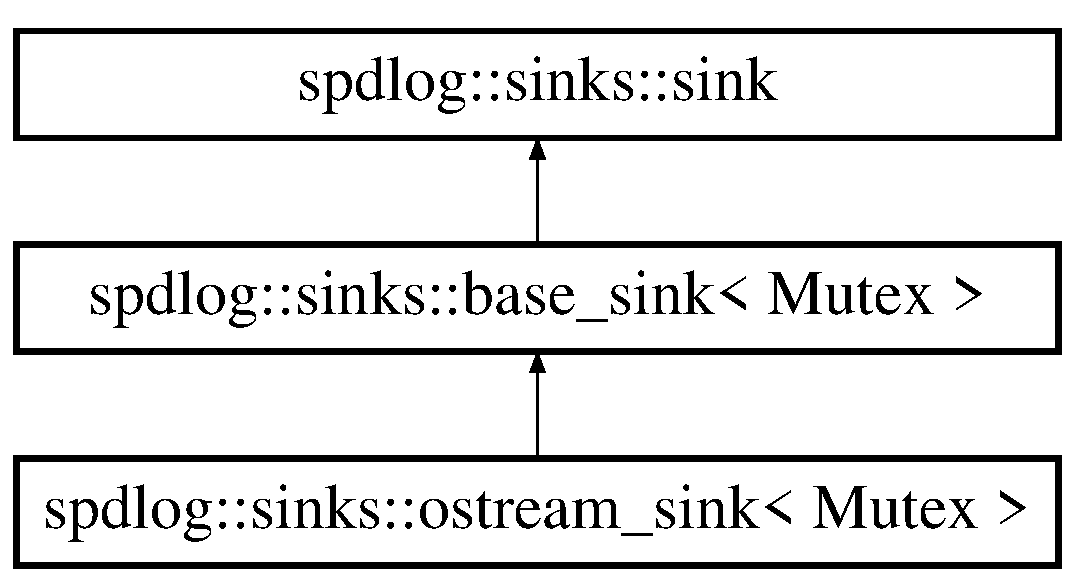
\includegraphics[height=3.000000cm]{classspdlog_1_1sinks_1_1ostream__sink}
\end{center}
\end{figure}
\subsection*{Public Member Functions}
\begin{DoxyCompactItemize}
\item 
{\bfseries ostream\+\_\+sink} (std\+::ostream \&os, bool force\+\_\+flush=false)\hypertarget{classspdlog_1_1sinks_1_1ostream__sink_aa038c6518dc69c08a1251e7469bc4fd8}{}\label{classspdlog_1_1sinks_1_1ostream__sink_aa038c6518dc69c08a1251e7469bc4fd8}

\item 
{\bfseries ostream\+\_\+sink} (const \hyperlink{classspdlog_1_1sinks_1_1ostream__sink}{ostream\+\_\+sink} \&)=delete\hypertarget{classspdlog_1_1sinks_1_1ostream__sink_a761f1c26210fe42673af4734b38fe167}{}\label{classspdlog_1_1sinks_1_1ostream__sink_a761f1c26210fe42673af4734b38fe167}

\item 
\hyperlink{classspdlog_1_1sinks_1_1ostream__sink}{ostream\+\_\+sink} \& {\bfseries operator=} (const \hyperlink{classspdlog_1_1sinks_1_1ostream__sink}{ostream\+\_\+sink} \&)=delete\hypertarget{classspdlog_1_1sinks_1_1ostream__sink_a727591b2a4ca044848cacccfca4eb3af}{}\label{classspdlog_1_1sinks_1_1ostream__sink_a727591b2a4ca044848cacccfca4eb3af}

\end{DoxyCompactItemize}
\subsection*{Protected Member Functions}
\begin{DoxyCompactItemize}
\item 
void {\bfseries \+\_\+sink\+\_\+it} (const \hyperlink{structspdlog_1_1details_1_1log__msg}{details\+::log\+\_\+msg} \&msg) override\hypertarget{classspdlog_1_1sinks_1_1ostream__sink_afa766b268315152fc4ed53c5d42907b3}{}\label{classspdlog_1_1sinks_1_1ostream__sink_afa766b268315152fc4ed53c5d42907b3}

\item 
void {\bfseries \+\_\+flush} () override\hypertarget{classspdlog_1_1sinks_1_1ostream__sink_a5d9f4f269c3ba7d279c224b91c2c6af7}{}\label{classspdlog_1_1sinks_1_1ostream__sink_a5d9f4f269c3ba7d279c224b91c2c6af7}

\end{DoxyCompactItemize}
\subsection*{Protected Attributes}
\begin{DoxyCompactItemize}
\item 
std\+::ostream \& {\bfseries \+\_\+ostream}\hypertarget{classspdlog_1_1sinks_1_1ostream__sink_a2007a7bade3e74b6a003ae27ed621c8f}{}\label{classspdlog_1_1sinks_1_1ostream__sink_a2007a7bade3e74b6a003ae27ed621c8f}

\item 
bool {\bfseries \+\_\+force\+\_\+flush}\hypertarget{classspdlog_1_1sinks_1_1ostream__sink_a9db02c29caf37c1e69e38d397006ae1f}{}\label{classspdlog_1_1sinks_1_1ostream__sink_a9db02c29caf37c1e69e38d397006ae1f}

\end{DoxyCompactItemize}


The documentation for this class was generated from the following file\+:\begin{DoxyCompactItemize}
\item 
cvdi-\/src/cvdi-\/cl/include/spdlog/sinks/ostream\+\_\+sink.\+h\end{DoxyCompactItemize}

\hypertarget{classMultiThread_1_1Parallel}{}\section{Multi\+Thread\+:\+:Parallel$<$ T $>$ Class Template Reference}
\label{classMultiThread_1_1Parallel}\index{Multi\+Thread\+::\+Parallel$<$ T $>$@{Multi\+Thread\+::\+Parallel$<$ T $>$}}
\subsection*{Public Member Functions}
\begin{DoxyCompactItemize}
\item 
void {\bfseries Start} (unsigned n\+\_\+threads)\hypertarget{classMultiThread_1_1Parallel_ae84be57a998a93293d74a501149a2731}{}\label{classMultiThread_1_1Parallel_ae84be57a998a93293d74a501149a2731}

\item 
virtual void {\bfseries Thread} (unsigned thread\+\_\+number, \hyperlink{classMultiThread_1_1SharedQueue}{Shared\+Queue}$<$ std\+::shared\+\_\+ptr$<$ T $>$$>$ $\ast$q)=0\hypertarget{classMultiThread_1_1Parallel_a1cfbbbbb3bbaa63437575a1b1e7467b1}{}\label{classMultiThread_1_1Parallel_a1cfbbbbb3bbaa63437575a1b1e7467b1}

\item 
virtual void {\bfseries Init} (unsigned n\+\_\+threads)=0\hypertarget{classMultiThread_1_1Parallel_a610be894ec3b79c02d377c767930d70f}{}\label{classMultiThread_1_1Parallel_a610be894ec3b79c02d377c767930d70f}

\item 
virtual void {\bfseries Close} (void)=0\hypertarget{classMultiThread_1_1Parallel_a5cd9d879caf11db0d36a2b82d7dd3459}{}\label{classMultiThread_1_1Parallel_a5cd9d879caf11db0d36a2b82d7dd3459}

\item 
virtual std\+::shared\+\_\+ptr$<$ T $>$ {\bfseries Next\+Item} (void)=0\hypertarget{classMultiThread_1_1Parallel_a78066be206baeece054d6dd1698ba3f5}{}\label{classMultiThread_1_1Parallel_a78066be206baeece054d6dd1698ba3f5}

\end{DoxyCompactItemize}


The documentation for this class was generated from the following file\+:\begin{DoxyCompactItemize}
\item 
cvdi-\/src/cvdi-\/cl/include/multi\+\_\+thread.\+hpp\end{DoxyCompactItemize}

\hypertarget{structcvdi_1_1PointCounter}{}\section{cvdi\+:\+:Point\+Counter Struct Reference}
\label{structcvdi_1_1PointCounter}\index{cvdi\+::\+Point\+Counter@{cvdi\+::\+Point\+Counter}}


A class to gather statistics about a trace.  




{\ttfamily \#include $<$cvdi.\+hpp$>$}

\subsection*{Public Member Functions}
\begin{DoxyCompactItemize}
\item 
\hyperlink{structcvdi_1_1PointCounter_a60c7c3b39c50542496711d133e543cdd}{Point\+Counter} ()
\begin{DoxyCompactList}\small\item\em \begin{quote}
The number of points in privacy intervals. \end{quote}
\end{DoxyCompactList}\item 
\hyperlink{structcvdi_1_1PointCounter_a615e1568bf8f36be3afc1e2c61654001}{Point\+Counter} (uint64\+\_\+t n\+\_\+points, uint64\+\_\+t \hyperlink{structcvdi_1_1PointCounter_ab329abe5fe52bd787dc2dc59afc03bc7}{n\+\_\+invalid\+\_\+field\+\_\+points}, uint64\+\_\+t \hyperlink{structcvdi_1_1PointCounter_abccc4d82bf51f4cac2f8eb03b71f6b31}{n\+\_\+invalid\+\_\+geo\+\_\+points}, uint64\+\_\+t \hyperlink{structcvdi_1_1PointCounter_ab051246dc41739c3f5133d58c6857617}{n\+\_\+invalid\+\_\+heading\+\_\+points}, uint64\+\_\+t \hyperlink{structcvdi_1_1PointCounter_a663df3cac0f4920c7a7afc8feb002f1d}{n\+\_\+ci\+\_\+points}, uint64\+\_\+t \hyperlink{structcvdi_1_1PointCounter_a6eda31fe450485d5a90403aa22dc51b9}{n\+\_\+pi\+\_\+points})
\begin{DoxyCompactList}\small\item\em Constructor with initialization of count values. \end{DoxyCompactList}\item 
\hyperlink{structcvdi_1_1PointCounter}{Point\+Counter} \hyperlink{structcvdi_1_1PointCounter_a274b6da1ad2f5afb2b7d7d2fb9adf1cd}{operator+} (const \hyperlink{structcvdi_1_1PointCounter}{Point\+Counter} \&other) const 
\begin{DoxyCompactList}\small\item\em Return a new \hyperlink{structcvdi_1_1PointCounter}{Point\+Counter} instance = this \hyperlink{structcvdi_1_1PointCounter}{Point\+Counter} + other \hyperlink{structcvdi_1_1PointCounter}{Point\+Counter}. Values in each \hyperlink{structcvdi_1_1PointCounter}{Point\+Counter} are added together. \end{DoxyCompactList}\end{DoxyCompactItemize}
\subsection*{Public Attributes}
\begin{DoxyCompactItemize}
\item 
uint64\+\_\+t {\bfseries n\+\_\+points}\hypertarget{structcvdi_1_1PointCounter_afbb269279caa378108ca6aa5f86042fe}{}\label{structcvdi_1_1PointCounter_afbb269279caa378108ca6aa5f86042fe}

\item 
uint64\+\_\+t \hyperlink{structcvdi_1_1PointCounter_ab329abe5fe52bd787dc2dc59afc03bc7}{n\+\_\+invalid\+\_\+field\+\_\+points}\hypertarget{structcvdi_1_1PointCounter_ab329abe5fe52bd787dc2dc59afc03bc7}{}\label{structcvdi_1_1PointCounter_ab329abe5fe52bd787dc2dc59afc03bc7}

\begin{DoxyCompactList}\small\item\em \begin{quote}
The number of points in a trace. \end{quote}
\end{DoxyCompactList}\item 
uint64\+\_\+t \hyperlink{structcvdi_1_1PointCounter_abccc4d82bf51f4cac2f8eb03b71f6b31}{n\+\_\+invalid\+\_\+geo\+\_\+points}\hypertarget{structcvdi_1_1PointCounter_abccc4d82bf51f4cac2f8eb03b71f6b31}{}\label{structcvdi_1_1PointCounter_abccc4d82bf51f4cac2f8eb03b71f6b31}

\begin{DoxyCompactList}\small\item\em \begin{quote}
The number of points with invalid field values. \end{quote}
\end{DoxyCompactList}\item 
uint64\+\_\+t \hyperlink{structcvdi_1_1PointCounter_ab051246dc41739c3f5133d58c6857617}{n\+\_\+invalid\+\_\+heading\+\_\+points}\hypertarget{structcvdi_1_1PointCounter_ab051246dc41739c3f5133d58c6857617}{}\label{structcvdi_1_1PointCounter_ab051246dc41739c3f5133d58c6857617}

\begin{DoxyCompactList}\small\item\em \begin{quote}
The number of points with invalid position. \end{quote}
\end{DoxyCompactList}\item 
uint64\+\_\+t \hyperlink{structcvdi_1_1PointCounter_a663df3cac0f4920c7a7afc8feb002f1d}{n\+\_\+ci\+\_\+points}\hypertarget{structcvdi_1_1PointCounter_a663df3cac0f4920c7a7afc8feb002f1d}{}\label{structcvdi_1_1PointCounter_a663df3cac0f4920c7a7afc8feb002f1d}

\begin{DoxyCompactList}\small\item\em \begin{quote}
The number of points with an invalid heading. \end{quote}
\end{DoxyCompactList}\item 
uint64\+\_\+t \hyperlink{structcvdi_1_1PointCounter_a6eda31fe450485d5a90403aa22dc51b9}{n\+\_\+pi\+\_\+points}\hypertarget{structcvdi_1_1PointCounter_a6eda31fe450485d5a90403aa22dc51b9}{}\label{structcvdi_1_1PointCounter_a6eda31fe450485d5a90403aa22dc51b9}

\begin{DoxyCompactList}\small\item\em \begin{quote}
The number of points in critical intervals. \end{quote}
\end{DoxyCompactList}\end{DoxyCompactItemize}
\subsection*{Friends}
\begin{DoxyCompactItemize}
\item 
std\+::ostream \& \hyperlink{structcvdi_1_1PointCounter_a7d38a9212813c666452f29a6bc89de6c}{operator$<$$<$} (std\+::ostream \&os, const \hyperlink{structcvdi_1_1PointCounter}{Point\+Counter} \&point\+\_\+counter)
\begin{DoxyCompactList}\small\item\em Write a \hyperlink{structcvdi_1_1PointCounter}{Point\+Counter} to an output stream. \end{DoxyCompactList}\end{DoxyCompactItemize}


\subsection{Detailed Description}
A class to gather statistics about a trace. 

\subsection{Constructor \& Destructor Documentation}
\index{cvdi\+::\+Point\+Counter@{cvdi\+::\+Point\+Counter}!Point\+Counter@{Point\+Counter}}
\index{Point\+Counter@{Point\+Counter}!cvdi\+::\+Point\+Counter@{cvdi\+::\+Point\+Counter}}
\subsubsection[{\texorpdfstring{Point\+Counter()}{PointCounter()}}]{\setlength{\rightskip}{0pt plus 5cm}cvdi\+::\+Point\+Counter\+::\+Point\+Counter (
\begin{DoxyParamCaption}
{}
\end{DoxyParamCaption}
)}\hypertarget{structcvdi_1_1PointCounter_a60c7c3b39c50542496711d133e543cdd}{}\label{structcvdi_1_1PointCounter_a60c7c3b39c50542496711d133e543cdd}


\begin{quote}
The number of points in privacy intervals. \end{quote}


Default constructor.

All statistics are initialized to 0. \index{cvdi\+::\+Point\+Counter@{cvdi\+::\+Point\+Counter}!Point\+Counter@{Point\+Counter}}
\index{Point\+Counter@{Point\+Counter}!cvdi\+::\+Point\+Counter@{cvdi\+::\+Point\+Counter}}
\subsubsection[{\texorpdfstring{Point\+Counter(uint64\+\_\+t n\+\_\+points, uint64\+\_\+t n\+\_\+invalid\+\_\+field\+\_\+points, uint64\+\_\+t n\+\_\+invalid\+\_\+geo\+\_\+points, uint64\+\_\+t n\+\_\+invalid\+\_\+heading\+\_\+points, uint64\+\_\+t n\+\_\+ci\+\_\+points, uint64\+\_\+t n\+\_\+pi\+\_\+points)}{PointCounter(uint64_t n_points, uint64_t n_invalid_field_points, uint64_t n_invalid_geo_points, uint64_t n_invalid_heading_points, uint64_t n_ci_points, uint64_t n_pi_points)}}]{\setlength{\rightskip}{0pt plus 5cm}cvdi\+::\+Point\+Counter\+::\+Point\+Counter (
\begin{DoxyParamCaption}
\item[{uint64\+\_\+t}]{n\+\_\+points, }
\item[{uint64\+\_\+t}]{n\+\_\+invalid\+\_\+field\+\_\+points, }
\item[{uint64\+\_\+t}]{n\+\_\+invalid\+\_\+geo\+\_\+points, }
\item[{uint64\+\_\+t}]{n\+\_\+invalid\+\_\+heading\+\_\+points, }
\item[{uint64\+\_\+t}]{n\+\_\+ci\+\_\+points, }
\item[{uint64\+\_\+t}]{n\+\_\+pi\+\_\+points}
\end{DoxyParamCaption}
)}\hypertarget{structcvdi_1_1PointCounter_a615e1568bf8f36be3afc1e2c61654001}{}\label{structcvdi_1_1PointCounter_a615e1568bf8f36be3afc1e2c61654001}


Constructor with initialization of count values. 


\begin{DoxyParams}{Parameters}
{\em n\+\_\+points} & initial number of point value \\
\hline
{\em n\+\_\+invalid\+\_\+field\+\_\+points} & initial number of points with invalid fields \\
\hline
{\em n\+\_\+invalid\+\_\+geo\+\_\+points} & initial number of points that have invalid G\+PS coordinates \\
\hline
{\em n\+\_\+invalid\+\_\+heading\+\_\+points} & initial number of points that have invalid headings \\
\hline
{\em n\+\_\+ci\+\_\+points} & initial number of points in a critical interval \\
\hline
{\em n\+\_\+pi\+\_\+points} & initial number of points in a privacy interval \\
\hline
\end{DoxyParams}


\subsection{Member Function Documentation}
\index{cvdi\+::\+Point\+Counter@{cvdi\+::\+Point\+Counter}!operator+@{operator+}}
\index{operator+@{operator+}!cvdi\+::\+Point\+Counter@{cvdi\+::\+Point\+Counter}}
\subsubsection[{\texorpdfstring{operator+(const Point\+Counter \&other) const }{operator+(const PointCounter &other) const }}]{\setlength{\rightskip}{0pt plus 5cm}{\bf Point\+Counter} cvdi\+::\+Point\+Counter\+::operator+ (
\begin{DoxyParamCaption}
\item[{const {\bf Point\+Counter} \&}]{other}
\end{DoxyParamCaption}
) const}\hypertarget{structcvdi_1_1PointCounter_a274b6da1ad2f5afb2b7d7d2fb9adf1cd}{}\label{structcvdi_1_1PointCounter_a274b6da1ad2f5afb2b7d7d2fb9adf1cd}


Return a new \hyperlink{structcvdi_1_1PointCounter}{Point\+Counter} instance = this \hyperlink{structcvdi_1_1PointCounter}{Point\+Counter} + other \hyperlink{structcvdi_1_1PointCounter}{Point\+Counter}. Values in each \hyperlink{structcvdi_1_1PointCounter}{Point\+Counter} are added together. 

This \hyperlink{structcvdi_1_1PointCounter}{Point\+Counter} is N\+OT modified.


\begin{DoxyParams}{Parameters}
{\em other} & the \hyperlink{structcvdi_1_1PointCounter}{Point\+Counter} whose value are to be added to this point counter \\
\hline
\end{DoxyParams}
\begin{DoxyReturn}{Returns}
a N\+EW \hyperlink{structcvdi_1_1PointCounter}{Point\+Counter} instance 
\end{DoxyReturn}


\subsection{Friends And Related Function Documentation}
\index{cvdi\+::\+Point\+Counter@{cvdi\+::\+Point\+Counter}!operator$<$$<$@{operator$<$$<$}}
\index{operator$<$$<$@{operator$<$$<$}!cvdi\+::\+Point\+Counter@{cvdi\+::\+Point\+Counter}}
\subsubsection[{\texorpdfstring{operator$<$$<$}{operator<<}}]{\setlength{\rightskip}{0pt plus 5cm}std\+::ostream\& operator$<$$<$ (
\begin{DoxyParamCaption}
\item[{std\+::ostream \&}]{os, }
\item[{const {\bf Point\+Counter} \&}]{point\+\_\+counter}
\end{DoxyParamCaption}
)\hspace{0.3cm}{\ttfamily [friend]}}\hypertarget{structcvdi_1_1PointCounter_a7d38a9212813c666452f29a6bc89de6c}{}\label{structcvdi_1_1PointCounter_a7d38a9212813c666452f29a6bc89de6c}


Write a \hyperlink{structcvdi_1_1PointCounter}{Point\+Counter} to an output stream. 

The form of the output is a comma-\/delimited list of the various values managed by the \hyperlink{structcvdi_1_1PointCounter}{Point\+Counter}.


\begin{DoxyParams}{Parameters}
{\em os} & the output stream to write the string form of this \hyperlink{structcvdi_1_1PointCounter}{Point\+Counter} \\
\hline
{\em point\+\_\+counter} & the \hyperlink{structcvdi_1_1PointCounter}{Point\+Counter} to write \\
\hline
\end{DoxyParams}
\begin{DoxyReturn}{Returns}
the output stream after the write 
\end{DoxyReturn}


The documentation for this struct was generated from the following files\+:\begin{DoxyCompactItemize}
\item 
cvdi-\/src/cvdi/include/cvdi.\+hpp\item 
cvdi-\/src/cvdi/src/cvdi.\+cpp\end{DoxyCompactItemize}

\hypertarget{classgeo__data_1_1PostGISRoadReader}{}\section{geo\+\_\+data\+:\+:Post\+G\+I\+S\+Road\+Reader Class Reference}
\label{classgeo__data_1_1PostGISRoadReader}\index{geo\+\_\+data\+::\+Post\+G\+I\+S\+Road\+Reader@{geo\+\_\+data\+::\+Post\+G\+I\+S\+Road\+Reader}}


Postgis (postgres) \hyperlink{classgeo__data_1_1RoadReader}{Road\+Reader}. Reads roads from the postgis O\+SM bfmap\+\_\+ways table of the database.  




{\ttfamily \#include $<$geo\+\_\+data.\+hpp$>$}

Inheritance diagram for geo\+\_\+data\+:\+:Post\+G\+I\+S\+Road\+Reader\+:\begin{figure}[H]
\begin{center}
\leavevmode
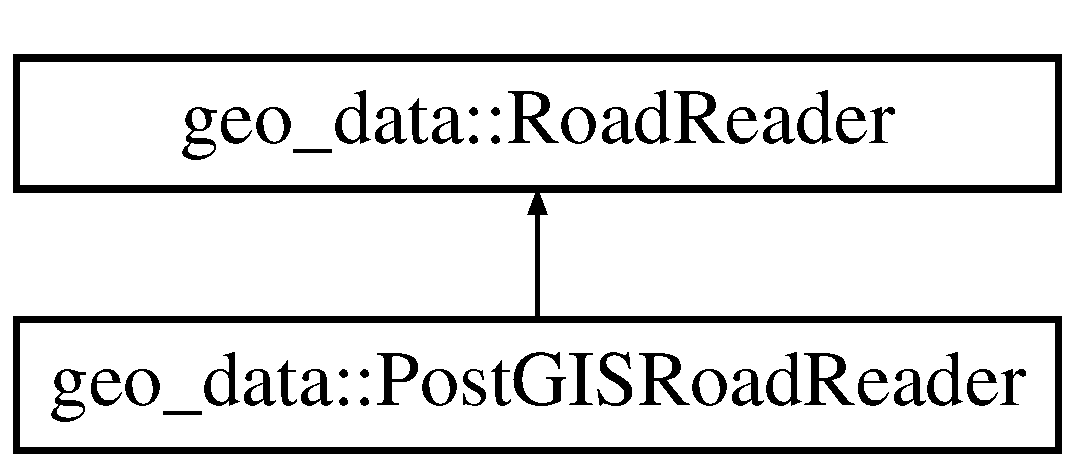
\includegraphics[height=2.000000cm]{classgeo__data_1_1PostGISRoadReader}
\end{center}
\end{figure}
\subsection*{Public Member Functions}
\begin{DoxyCompactItemize}
\item 
\hyperlink{classgeo__data_1_1PostGISRoadReader_ad45dbce658a641c26137fc04eb2b34e2}{Post\+G\+I\+S\+Road\+Reader} (const std\+::string \&host, uint32\+\_\+t port, const std\+::string \&database, const std\+::string \&user, const std\+::string \&password, const O\+S\+M\+Config\+Map \&osm\+\_\+config\+\_\+map\+\_\+)
\begin{DoxyCompactList}\small\item\em Construct a \hyperlink{classgeo__data_1_1PostGISRoadReader}{Post\+G\+I\+S\+Road\+Reader} object. \end{DoxyCompactList}\item 
\hyperlink{classgeo__data_1_1PostGISRoadReader_aaa5ee860cdc35c2fbc988520859efcbd}{$\sim$\+Post\+G\+I\+S\+Road\+Reader} ()\hypertarget{classgeo__data_1_1PostGISRoadReader_aaa5ee860cdc35c2fbc988520859efcbd}{}\label{classgeo__data_1_1PostGISRoadReader_aaa5ee860cdc35c2fbc988520859efcbd}

\begin{DoxyCompactList}\small\item\em Destruct a \hyperlink{classgeo__data_1_1PostGISRoadReader}{Post\+G\+I\+S\+Road\+Reader} object. \end{DoxyCompactList}\item 
geo\+::\+Road\+::\+Ptr \hyperlink{classgeo__data_1_1PostGISRoadReader_aafd2e9afed093d19550677e91f4cfec2}{next\+\_\+road} (void)
\begin{DoxyCompactList}\small\item\em Get the next road from the O\+SM bfmap\+\_\+ways table query. \end{DoxyCompactList}\end{DoxyCompactItemize}
\subsection*{Additional Inherited Members}


\subsection{Detailed Description}
Postgis (postgres) \hyperlink{classgeo__data_1_1RoadReader}{Road\+Reader}. Reads roads from the postgis O\+SM bfmap\+\_\+ways table of the database. 

\subsection{Constructor \& Destructor Documentation}
\index{geo\+\_\+data\+::\+Post\+G\+I\+S\+Road\+Reader@{geo\+\_\+data\+::\+Post\+G\+I\+S\+Road\+Reader}!Post\+G\+I\+S\+Road\+Reader@{Post\+G\+I\+S\+Road\+Reader}}
\index{Post\+G\+I\+S\+Road\+Reader@{Post\+G\+I\+S\+Road\+Reader}!geo\+\_\+data\+::\+Post\+G\+I\+S\+Road\+Reader@{geo\+\_\+data\+::\+Post\+G\+I\+S\+Road\+Reader}}
\subsubsection[{\texorpdfstring{Post\+G\+I\+S\+Road\+Reader(const std\+::string \&host, uint32\+\_\+t port, const std\+::string \&database, const std\+::string \&user, const std\+::string \&password, const O\+S\+M\+Config\+Map \&osm\+\_\+config\+\_\+map\+\_\+)}{PostGISRoadReader(const std::string &host, uint32_t port, const std::string &database, const std::string &user, const std::string &password, const OSMConfigMap &osm_config_map_)}}]{\setlength{\rightskip}{0pt plus 5cm}geo\+\_\+data\+::\+Post\+G\+I\+S\+Road\+Reader\+::\+Post\+G\+I\+S\+Road\+Reader (
\begin{DoxyParamCaption}
\item[{const std\+::string \&}]{host, }
\item[{uint32\+\_\+t}]{port, }
\item[{const std\+::string \&}]{database, }
\item[{const std\+::string \&}]{user, }
\item[{const std\+::string \&}]{password, }
\item[{const O\+S\+M\+Config\+Map \&}]{osm\+\_\+config\+\_\+map\+\_\+}
\end{DoxyParamCaption}
)}\hypertarget{classgeo__data_1_1PostGISRoadReader_ad45dbce658a641c26137fc04eb2b34e2}{}\label{classgeo__data_1_1PostGISRoadReader_ad45dbce658a641c26137fc04eb2b34e2}


Construct a \hyperlink{classgeo__data_1_1PostGISRoadReader}{Post\+G\+I\+S\+Road\+Reader} object. 


\begin{DoxyParams}{Parameters}
{\em host} & the address or F\+Q\+DN of the postgres host \\
\hline
{\em port} & the port the where the postgres server is running \\
\hline
{\em database} & the name of O\+SM road network database \\
\hline
{\em user} & the name of the postgres user \\
\hline
{\em password} & the password for the postgres user \\
\hline
{\em osm\+\_\+config\+\_\+map} & configuration for O\+SM ways \\
\hline
\end{DoxyParams}

\begin{DoxyExceptions}{Exceptions}
{\em std\+::invalid\+\_\+argument} & if the psotgres connection could not be established or the query fails \\
\hline
\end{DoxyExceptions}


\subsection{Member Function Documentation}
\index{geo\+\_\+data\+::\+Post\+G\+I\+S\+Road\+Reader@{geo\+\_\+data\+::\+Post\+G\+I\+S\+Road\+Reader}!next\+\_\+road@{next\+\_\+road}}
\index{next\+\_\+road@{next\+\_\+road}!geo\+\_\+data\+::\+Post\+G\+I\+S\+Road\+Reader@{geo\+\_\+data\+::\+Post\+G\+I\+S\+Road\+Reader}}
\subsubsection[{\texorpdfstring{next\+\_\+road(void)}{next_road(void)}}]{\setlength{\rightskip}{0pt plus 5cm}geo\+::\+Road\+::\+Ptr geo\+\_\+data\+::\+Post\+G\+I\+S\+Road\+Reader\+::next\+\_\+road (
\begin{DoxyParamCaption}
\item[{void}]{}
\end{DoxyParamCaption}
)\hspace{0.3cm}{\ttfamily [virtual]}}\hypertarget{classgeo__data_1_1PostGISRoadReader_aafd2e9afed093d19550677e91f4cfec2}{}\label{classgeo__data_1_1PostGISRoadReader_aafd2e9afed093d19550677e91f4cfec2}


Get the next road from the O\+SM bfmap\+\_\+ways table query. 

\begin{DoxyReturn}{Returns}
a pointer to \hyperlink{classgeo_1_1Road}{geo\+::\+Road} or nullptr if there are no more roads 
\end{DoxyReturn}


Implements \hyperlink{classgeo__data_1_1RoadReader}{geo\+\_\+data\+::\+Road\+Reader}.



The documentation for this class was generated from the following files\+:\begin{DoxyCompactItemize}
\item 
cvdi-\/src/geo-\/data/include/geo\+\_\+data.\+hpp\item 
cvdi-\/src/geo-\/data/src/geo\+\_\+data.\+cpp\end{DoxyCompactItemize}

\hypertarget{classfmt_1_1internal_1_1PrintfArgFormatter}{}\section{fmt\+:\+:internal\+:\+:Printf\+Arg\+Formatter$<$ Char $>$ Class Template Reference}
\label{classfmt_1_1internal_1_1PrintfArgFormatter}\index{fmt\+::internal\+::\+Printf\+Arg\+Formatter$<$ Char $>$@{fmt\+::internal\+::\+Printf\+Arg\+Formatter$<$ Char $>$}}
Inheritance diagram for fmt\+:\+:internal\+:\+:Printf\+Arg\+Formatter$<$ Char $>$\+:\begin{figure}[H]
\begin{center}
\leavevmode
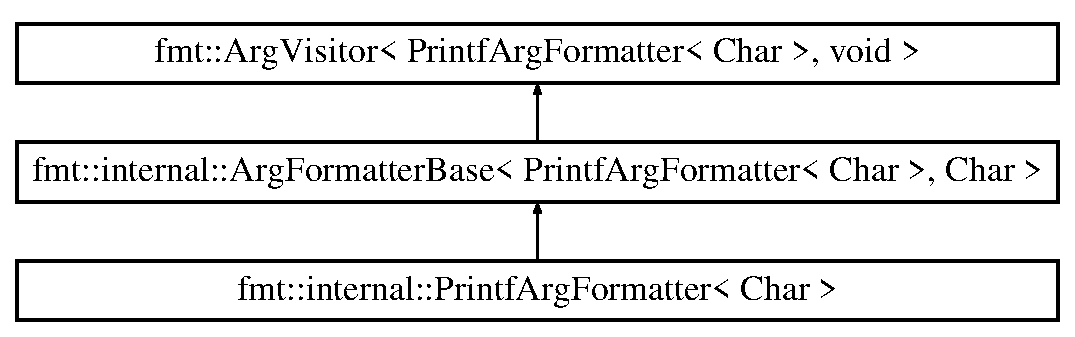
\includegraphics[height=3.000000cm]{classfmt_1_1internal_1_1PrintfArgFormatter}
\end{center}
\end{figure}
\subsection*{Public Member Functions}
\begin{DoxyCompactItemize}
\item 
{\bfseries Printf\+Arg\+Formatter} (\hyperlink{classfmt_1_1BasicWriter}{Basic\+Writer}$<$ Char $>$ \&w, \hyperlink{structfmt_1_1FormatSpec}{Format\+Spec} \&s)\hypertarget{classfmt_1_1internal_1_1PrintfArgFormatter_add5c9219de52b2e2f5d65d2736c7c9bf}{}\label{classfmt_1_1internal_1_1PrintfArgFormatter_add5c9219de52b2e2f5d65d2736c7c9bf}

\item 
void {\bfseries visit\+\_\+bool} (bool value)\hypertarget{classfmt_1_1internal_1_1PrintfArgFormatter_a9bbc1d48d1e781f9a15c5a94161bc8cb}{}\label{classfmt_1_1internal_1_1PrintfArgFormatter_a9bbc1d48d1e781f9a15c5a94161bc8cb}

\item 
void {\bfseries visit\+\_\+char} (int value)\hypertarget{classfmt_1_1internal_1_1PrintfArgFormatter_a17e33efa05145a8bd040ded42a1be92b}{}\label{classfmt_1_1internal_1_1PrintfArgFormatter_a17e33efa05145a8bd040ded42a1be92b}

\item 
void {\bfseries visit\+\_\+cstring} (const char $\ast$value)\hypertarget{classfmt_1_1internal_1_1PrintfArgFormatter_aecc9a8257acaa9e47fac68e7a4c02592}{}\label{classfmt_1_1internal_1_1PrintfArgFormatter_aecc9a8257acaa9e47fac68e7a4c02592}

\item 
void {\bfseries visit\+\_\+pointer} (const void $\ast$value)\hypertarget{classfmt_1_1internal_1_1PrintfArgFormatter_ad2915cafb93887054479120089d31421}{}\label{classfmt_1_1internal_1_1PrintfArgFormatter_ad2915cafb93887054479120089d31421}

\item 
void {\bfseries visit\+\_\+custom} (\hyperlink{structfmt_1_1internal_1_1Value_1_1CustomValue}{Arg\+::\+Custom\+Value} c)\hypertarget{classfmt_1_1internal_1_1PrintfArgFormatter_ab3f93bc2476db68b7f3e2a5530a57916}{}\label{classfmt_1_1internal_1_1PrintfArgFormatter_ab3f93bc2476db68b7f3e2a5530a57916}

\end{DoxyCompactItemize}
\subsection*{Additional Inherited Members}


The documentation for this class was generated from the following file\+:\begin{DoxyCompactItemize}
\item 
cvdi-\/src/cvdi-\/cl/include/spdlog/fmt/bundled/format.\+cc\end{DoxyCompactItemize}

\hypertarget{classfmt_1_1internal_1_1PrintfFormatter}{}\section{fmt\+:\+:internal\+:\+:Printf\+Formatter$<$ Char $>$ Class Template Reference}
\label{classfmt_1_1internal_1_1PrintfFormatter}\index{fmt\+::internal\+::\+Printf\+Formatter$<$ Char $>$@{fmt\+::internal\+::\+Printf\+Formatter$<$ Char $>$}}
Inheritance diagram for fmt\+:\+:internal\+:\+:Printf\+Formatter$<$ Char $>$\+:\begin{figure}[H]
\begin{center}
\leavevmode
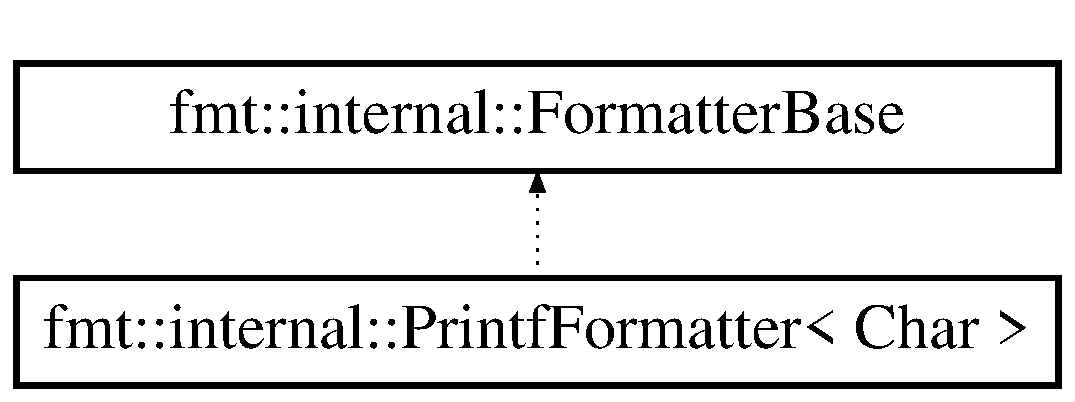
\includegraphics[height=2.000000cm]{classfmt_1_1internal_1_1PrintfFormatter}
\end{center}
\end{figure}
\subsection*{Public Member Functions}
\begin{DoxyCompactItemize}
\item 
{\bfseries Printf\+Formatter} (const \hyperlink{classfmt_1_1ArgList}{Arg\+List} \&args)\hypertarget{classfmt_1_1internal_1_1PrintfFormatter_a4477dcf12266b16a27077ec4fdc20f45}{}\label{classfmt_1_1internal_1_1PrintfFormatter_a4477dcf12266b16a27077ec4fdc20f45}

\item 
F\+M\+T\+\_\+\+A\+PI void {\bfseries format} (\hyperlink{classfmt_1_1BasicWriter}{Basic\+Writer}$<$ Char $>$ \&writer, \hyperlink{classfmt_1_1BasicCStringRef}{Basic\+C\+String\+Ref}$<$ Char $>$ format\+\_\+str)\hypertarget{classfmt_1_1internal_1_1PrintfFormatter_a8b87898afca8f347fe5242f6d2b0ac60}{}\label{classfmt_1_1internal_1_1PrintfFormatter_a8b87898afca8f347fe5242f6d2b0ac60}

\end{DoxyCompactItemize}


The documentation for this class was generated from the following files\+:\begin{DoxyCompactItemize}
\item 
cvdi-\/src/cvdi-\/cl/include/spdlog/fmt/bundled/format.\+h\item 
cvdi-\/src/cvdi-\/cl/include/spdlog/fmt/bundled/format.\+cc\end{DoxyCompactItemize}

\hypertarget{classcvdi_1_1PrivacyIntervalFinder}{}\section{cvdi\+:\+:Privacy\+Interval\+Finder Class Reference}
\label{classcvdi_1_1PrivacyIntervalFinder}\index{cvdi\+::\+Privacy\+Interval\+Finder@{cvdi\+::\+Privacy\+Interval\+Finder}}


Define the intervals that \char`\"{}hide\char`\"{} critical intervals. Instances of this class determine the portion of a trace extended from the ends of the previously defined critical intervals to protect those locations. This is done using intersection out degree, direct distance, and Manhattan distance.  




{\ttfamily \#include $<$cvdi.\+hpp$>$}

\subsection*{Public Types}
\begin{DoxyCompactItemize}
\item 
using {\bfseries Trajectory\+Iterator} = geo\+\_\+data\+::\+Sample\+::\+Trace\+::iterator\hypertarget{classcvdi_1_1PrivacyIntervalFinder_a82dfa8f6018349f3e430fd842e2a17cc}{}\label{classcvdi_1_1PrivacyIntervalFinder_a82dfa8f6018349f3e430fd842e2a17cc}

\item 
using {\bfseries Rev\+Trajectory\+Iterator} = geo\+\_\+data\+::\+Sample\+::\+Trace\+::reverse\+\_\+iterator\hypertarget{classcvdi_1_1PrivacyIntervalFinder_aed4483689c32d185a5fa2f5c7d387700}{}\label{classcvdi_1_1PrivacyIntervalFinder_aed4483689c32d185a5fa2f5c7d387700}

\end{DoxyCompactItemize}
\subsection*{Public Member Functions}
\begin{DoxyCompactItemize}
\item 
\hyperlink{classcvdi_1_1PrivacyIntervalFinder_ae7041f26e25befc38dc63771c901ff47}{Privacy\+Interval\+Finder} (double min\+\_\+dd, double min\+\_\+md, uint32\+\_\+t min\+\_\+out\+\_\+degree, double max\+\_\+dd, double max\+\_\+md, uint32\+\_\+t max\+\_\+out\+\_\+degree, double dd\+\_\+rand, double md\+\_\+rand, double out\+\_\+degree\+\_\+rand)
\begin{DoxyCompactList}\small\item\em Construct a \hyperlink{classcvdi_1_1PrivacyIntervalFinder}{Privacy\+Interval\+Finder} object. \end{DoxyCompactList}\item 
const geo\+\_\+data\+::\+Interval\+::\+Ptr\+List \& \hyperlink{classcvdi_1_1PrivacyIntervalFinder_af41665ec45983014303ec2124038308e}{find\+\_\+intervals} (geo\+\_\+data\+::\+Sample\+::\+Trace \&trace)
\begin{DoxyCompactList}\small\item\em Find the privacy intervals in the provided trace. \end{DoxyCompactList}\end{DoxyCompactItemize}


\subsection{Detailed Description}
Define the intervals that \char`\"{}hide\char`\"{} critical intervals. Instances of this class determine the portion of a trace extended from the ends of the previously defined critical intervals to protect those locations. This is done using intersection out degree, direct distance, and Manhattan distance. 

\subsection{Constructor \& Destructor Documentation}
\index{cvdi\+::\+Privacy\+Interval\+Finder@{cvdi\+::\+Privacy\+Interval\+Finder}!Privacy\+Interval\+Finder@{Privacy\+Interval\+Finder}}
\index{Privacy\+Interval\+Finder@{Privacy\+Interval\+Finder}!cvdi\+::\+Privacy\+Interval\+Finder@{cvdi\+::\+Privacy\+Interval\+Finder}}
\subsubsection[{\texorpdfstring{Privacy\+Interval\+Finder(double min\+\_\+dd, double min\+\_\+md, uint32\+\_\+t min\+\_\+out\+\_\+degree, double max\+\_\+dd, double max\+\_\+md, uint32\+\_\+t max\+\_\+out\+\_\+degree, double dd\+\_\+rand, double md\+\_\+rand, double out\+\_\+degree\+\_\+rand)}{PrivacyIntervalFinder(double min_dd, double min_md, uint32_t min_out_degree, double max_dd, double max_md, uint32_t max_out_degree, double dd_rand, double md_rand, double out_degree_rand)}}]{\setlength{\rightskip}{0pt plus 5cm}cvdi\+::\+Privacy\+Interval\+Finder\+::\+Privacy\+Interval\+Finder (
\begin{DoxyParamCaption}
\item[{double}]{min\+\_\+dd, }
\item[{double}]{min\+\_\+md, }
\item[{uint32\+\_\+t}]{min\+\_\+out\+\_\+degree, }
\item[{double}]{max\+\_\+dd, }
\item[{double}]{max\+\_\+md, }
\item[{uint32\+\_\+t}]{max\+\_\+out\+\_\+degree, }
\item[{double}]{dd\+\_\+rand, }
\item[{double}]{md\+\_\+rand, }
\item[{double}]{out\+\_\+degree\+\_\+rand}
\end{DoxyParamCaption}
)}\hypertarget{classcvdi_1_1PrivacyIntervalFinder_ae7041f26e25befc38dc63771c901ff47}{}\label{classcvdi_1_1PrivacyIntervalFinder_ae7041f26e25befc38dc63771c901ff47}


Construct a \hyperlink{classcvdi_1_1PrivacyIntervalFinder}{Privacy\+Interval\+Finder} object. 


\begin{DoxyParams}{Parameters}
{\em min\+\_\+dd} & minimum direct distance \\
\hline
{\em min\+\_\+md} & minimum manhattan distance \\
\hline
{\em min\+\_\+out\+\_\+degree} & minimum intersection out degree \\
\hline
{\em max\+\_\+dd} & maximum direct distance \\
\hline
{\em max\+\_\+md} & maximum manhattan distance \\
\hline
{\em max\+\_\+out\+\_\+degree} & maximum intersection out degree \\
\hline
{\em dd\+\_\+rand} & direct distance randomization factor \\
\hline
{\em md\+\_\+rand} & manhattan distance randomization factor \\
\hline
{\em out\+\_\+degree\+\_\+rand} & out degree randomization factor \\
\hline
\end{DoxyParams}


\subsection{Member Function Documentation}
\index{cvdi\+::\+Privacy\+Interval\+Finder@{cvdi\+::\+Privacy\+Interval\+Finder}!find\+\_\+intervals@{find\+\_\+intervals}}
\index{find\+\_\+intervals@{find\+\_\+intervals}!cvdi\+::\+Privacy\+Interval\+Finder@{cvdi\+::\+Privacy\+Interval\+Finder}}
\subsubsection[{\texorpdfstring{find\+\_\+intervals(geo\+\_\+data\+::\+Sample\+::\+Trace \&trace)}{find_intervals(geo_data::Sample::Trace &trace)}}]{\setlength{\rightskip}{0pt plus 5cm}const geo\+\_\+data\+::\+Interval\+::\+Ptr\+List \& cvdi\+::\+Privacy\+Interval\+Finder\+::find\+\_\+intervals (
\begin{DoxyParamCaption}
\item[{geo\+\_\+data\+::\+Sample\+::\+Trace \&}]{trace}
\end{DoxyParamCaption}
)}\hypertarget{classcvdi_1_1PrivacyIntervalFinder_af41665ec45983014303ec2124038308e}{}\label{classcvdi_1_1PrivacyIntervalFinder_af41665ec45983014303ec2124038308e}


Find the privacy intervals in the provided trace. 


\begin{DoxyParams}{Parameters}
{\em trace} & the trace to search for privacy intervals \\
\hline
\end{DoxyParams}
\begin{DoxyReturn}{Returns}
a list of the intervals that define the privacy intervals 
\end{DoxyReturn}


The documentation for this class was generated from the following files\+:\begin{DoxyCompactItemize}
\item 
cvdi-\/src/cvdi/include/cvdi.\+hpp\item 
cvdi-\/src/cvdi/src/cvdi.\+cpp\end{DoxyCompactItemize}

\hypertarget{classspdlog_1_1details_1_1registry__t}{}\section{spdlog\+:\+:details\+:\+:registry\+\_\+t$<$ Mutex $>$ Class Template Reference}
\label{classspdlog_1_1details_1_1registry__t}\index{spdlog\+::details\+::registry\+\_\+t$<$ Mutex $>$@{spdlog\+::details\+::registry\+\_\+t$<$ Mutex $>$}}
\subsection*{Public Member Functions}
\begin{DoxyCompactItemize}
\item 
void {\bfseries register\+\_\+logger} (std\+::shared\+\_\+ptr$<$ \hyperlink{classspdlog_1_1logger}{logger} $>$ \hyperlink{classspdlog_1_1logger}{logger})\hypertarget{classspdlog_1_1details_1_1registry__t_a75c112598c85eeadce7eaa2babe42f6a}{}\label{classspdlog_1_1details_1_1registry__t_a75c112598c85eeadce7eaa2babe42f6a}

\item 
std\+::shared\+\_\+ptr$<$ \hyperlink{classspdlog_1_1logger}{logger} $>$ {\bfseries get} (const std\+::string \&logger\+\_\+name)\hypertarget{classspdlog_1_1details_1_1registry__t_a83c60ec97a96497a28b29ec042e54103}{}\label{classspdlog_1_1details_1_1registry__t_a83c60ec97a96497a28b29ec042e54103}

\item 
{\footnotesize template$<$class It $>$ }\\std\+::shared\+\_\+ptr$<$ \hyperlink{classspdlog_1_1logger}{logger} $>$ {\bfseries create} (const std\+::string \&logger\+\_\+name, const It \&sinks\+\_\+begin, const It \&sinks\+\_\+end)\hypertarget{classspdlog_1_1details_1_1registry__t_a001d70ea4b0a4794dc4ffe2cdf720d22}{}\label{classspdlog_1_1details_1_1registry__t_a001d70ea4b0a4794dc4ffe2cdf720d22}

\item 
void {\bfseries apply\+\_\+all} (std\+::function$<$ void(std\+::shared\+\_\+ptr$<$ \hyperlink{classspdlog_1_1logger}{logger} $>$)$>$ fun)\hypertarget{classspdlog_1_1details_1_1registry__t_a6a75f3d36f7c54268512c586f4eb37af}{}\label{classspdlog_1_1details_1_1registry__t_a6a75f3d36f7c54268512c586f4eb37af}

\item 
void {\bfseries drop} (const std\+::string \&logger\+\_\+name)\hypertarget{classspdlog_1_1details_1_1registry__t_a547ea68afabdf2be39e20fa5aadbc37c}{}\label{classspdlog_1_1details_1_1registry__t_a547ea68afabdf2be39e20fa5aadbc37c}

\item 
void {\bfseries drop\+\_\+all} ()\hypertarget{classspdlog_1_1details_1_1registry__t_acd8ee16fd87c4f976a5728d4138acb2c}{}\label{classspdlog_1_1details_1_1registry__t_acd8ee16fd87c4f976a5728d4138acb2c}

\item 
std\+::shared\+\_\+ptr$<$ \hyperlink{classspdlog_1_1logger}{logger} $>$ {\bfseries create} (const std\+::string \&logger\+\_\+name, sinks\+\_\+init\+\_\+list sinks)\hypertarget{classspdlog_1_1details_1_1registry__t_ae3da0fbf3566bc5d6a27ec6a96f8c270}{}\label{classspdlog_1_1details_1_1registry__t_ae3da0fbf3566bc5d6a27ec6a96f8c270}

\item 
std\+::shared\+\_\+ptr$<$ \hyperlink{classspdlog_1_1logger}{logger} $>$ {\bfseries create} (const std\+::string \&logger\+\_\+name, sink\+\_\+ptr sink)\hypertarget{classspdlog_1_1details_1_1registry__t_acc516bff6719f15c33760d7771c70997}{}\label{classspdlog_1_1details_1_1registry__t_acc516bff6719f15c33760d7771c70997}

\item 
void {\bfseries formatter} (formatter\+\_\+ptr f)\hypertarget{classspdlog_1_1details_1_1registry__t_a23ab301e7663abdb8cc8ce1009450c7a}{}\label{classspdlog_1_1details_1_1registry__t_a23ab301e7663abdb8cc8ce1009450c7a}

\item 
void {\bfseries set\+\_\+pattern} (const std\+::string \&pattern)\hypertarget{classspdlog_1_1details_1_1registry__t_a96c915001a1b6c5656af1fd560fdec16}{}\label{classspdlog_1_1details_1_1registry__t_a96c915001a1b6c5656af1fd560fdec16}

\item 
void {\bfseries set\+\_\+level} (level\+::level\+\_\+enum log\+\_\+level)\hypertarget{classspdlog_1_1details_1_1registry__t_aabdbf66a65e1026e5e0dcbea877ff3ef}{}\label{classspdlog_1_1details_1_1registry__t_aabdbf66a65e1026e5e0dcbea877ff3ef}

\item 
void {\bfseries set\+\_\+error\+\_\+handler} (log\+\_\+err\+\_\+handler handler)\hypertarget{classspdlog_1_1details_1_1registry__t_a8cc9acbfcef9943cbff6611930d6c48c}{}\label{classspdlog_1_1details_1_1registry__t_a8cc9acbfcef9943cbff6611930d6c48c}

\item 
void {\bfseries set\+\_\+async\+\_\+mode} (size\+\_\+t q\+\_\+size, const async\+\_\+overflow\+\_\+policy overflow\+\_\+policy, const std\+::function$<$ void()$>$ \&worker\+\_\+warmup\+\_\+cb, const std\+::chrono\+::milliseconds \&flush\+\_\+interval\+\_\+ms, const std\+::function$<$ void()$>$ \&worker\+\_\+teardown\+\_\+cb)\hypertarget{classspdlog_1_1details_1_1registry__t_a0b2fec9af99edf72e3bc60a69fde5ba6}{}\label{classspdlog_1_1details_1_1registry__t_a0b2fec9af99edf72e3bc60a69fde5ba6}

\item 
void {\bfseries set\+\_\+sync\+\_\+mode} ()\hypertarget{classspdlog_1_1details_1_1registry__t_ad4aa99fcb43a890d9c64f8b0a88b829c}{}\label{classspdlog_1_1details_1_1registry__t_ad4aa99fcb43a890d9c64f8b0a88b829c}

\end{DoxyCompactItemize}
\subsection*{Static Public Member Functions}
\begin{DoxyCompactItemize}
\item 
static \hyperlink{classspdlog_1_1details_1_1registry__t}{registry\+\_\+t}$<$ Mutex $>$ \& {\bfseries instance} ()\hypertarget{classspdlog_1_1details_1_1registry__t_ad9730643a6d028115fc26937e6085d5c}{}\label{classspdlog_1_1details_1_1registry__t_ad9730643a6d028115fc26937e6085d5c}

\end{DoxyCompactItemize}


The documentation for this class was generated from the following file\+:\begin{DoxyCompactItemize}
\item 
cvdi-\/src/cvdi-\/cl/include/spdlog/details/registry.\+h\end{DoxyCompactItemize}

\hypertarget{classgeo_1_1Road}{}\section{geo\+:\+:Road Class Reference}
\label{classgeo_1_1Road}\index{geo\+::\+Road@{geo\+::\+Road}}


\hyperlink{classgeo_1_1Road}{Road} object containing a basic line string and meta data associated with the underlying real world road. A road can be one or two way and is used in spatial indexing. A road should not be confused with an edge used in the graph topology.  




{\ttfamily \#include $<$geo.\+hpp$>$}

\subsection*{Public Types}
\begin{DoxyCompactItemize}
\item 
using {\bfseries Ptr} = std\+::shared\+\_\+ptr$<$ \hyperlink{classgeo_1_1Road}{Road} $>$\hypertarget{classgeo_1_1Road_a1bd5a576d8c09aa43ae8b638f2e896de}{}\label{classgeo_1_1Road_a1bd5a576d8c09aa43ae8b638f2e896de}

\end{DoxyCompactItemize}
\subsection*{Public Member Functions}
\begin{DoxyCompactItemize}
\item 
\hyperlink{classgeo_1_1Road_a85b7e3e89e52e842bfa15e5404fe4a9e}{Road} (long gid, long \hyperlink{classgeo_1_1Road_a79fa381411ec36822a72b18bdc0fb208}{osm\+\_\+id}, long \hyperlink{classgeo_1_1Road_aeb43e9d82bbcab6a14a34abb749c4315}{source}, long \hyperlink{classgeo_1_1Road_adc5ce304928ae25948a4e4d96f239751}{target}, double reverse, long class\+\_\+id, float \hyperlink{classgeo_1_1Road_a24e121011f2b204e1d591c6a4f886380}{priority}, int \hyperlink{classgeo_1_1Road_a08506729380f0ec23720cffd27ea3d16}{maxspeed\+\_\+forward}, int \hyperlink{classgeo_1_1Road_a4278e486912e378390de155ca0bb2fc9}{maxspeed\+\_\+backward}, double \hyperlink{classgeo_1_1Road_ad102794fac433fc684647827d79f0aeb}{width}, bool \hyperlink{classgeo_1_1Road_afdc7c8bacdac2e5976bf29a0e9ee5ce2}{is\+\_\+excluded}, const std\+::string geom\+\_\+string, bool \hyperlink{classgeo_1_1Road_a63163ca614d9d01b3e15bf06a0901ddb}{is\+\_\+valid}=true, const std\+::string \hyperlink{classgeo_1_1Road_a32af3119496e802b14d9b1e3529b139b}{error\+\_\+msg}=\char`\"{}\char`\"{})
\begin{DoxyCompactList}\small\item\em Construct a road. Most fields are copied to the new object. The geometric string is used to build the underlying line string. This string should be a valid W\+KB representation of a line string, otherwise the road will be set to invalid. This also constructs a bounds for this road so that it can be spatially indexed (e.\+g. by a quad tree). \end{DoxyCompactList}\item 
long \hyperlink{classgeo_1_1Road_a2461a5c785065220b6036f9e2e6646ff}{id} () const 
\begin{DoxyCompactList}\small\item\em Get the unique ID of this road. \end{DoxyCompactList}\item 
long \hyperlink{classgeo_1_1Road_a79fa381411ec36822a72b18bdc0fb208}{osm\+\_\+id} () const 
\begin{DoxyCompactList}\small\item\em Get the O\+SM way ID of this road. \end{DoxyCompactList}\item 
long \hyperlink{classgeo_1_1Road_aeb43e9d82bbcab6a14a34abb749c4315}{source} () const 
\begin{DoxyCompactList}\small\item\em Get the ID of the source vertex of this road. \end{DoxyCompactList}\item 
long \hyperlink{classgeo_1_1Road_adc5ce304928ae25948a4e4d96f239751}{target} () const 
\begin{DoxyCompactList}\small\item\em Get the ID of the target vertex of this road. \end{DoxyCompactList}\item 
long \hyperlink{classgeo_1_1Road_a22e7817a996ae5367f549228bbdda1b9}{type} () const 
\begin{DoxyCompactList}\small\item\em Get the O\+SM way type of this road. \end{DoxyCompactList}\item 
long \hyperlink{classgeo_1_1Road_a08506729380f0ec23720cffd27ea3d16}{maxspeed\+\_\+forward} () const 
\begin{DoxyCompactList}\small\item\em Get the maximum forward speed for the road as kilometers per hour. \end{DoxyCompactList}\item 
long \hyperlink{classgeo_1_1Road_a4278e486912e378390de155ca0bb2fc9}{maxspeed\+\_\+backward} () const 
\begin{DoxyCompactList}\small\item\em Get the maximum backward speed for the road as kilometers per hour. \end{DoxyCompactList}\item 
double \hyperlink{classgeo_1_1Road_ae8ac2aa49e88d8698fac37e74d07b829}{length} () const 
\begin{DoxyCompactList}\small\item\em Get the length of this road in meters. \end{DoxyCompactList}\item 
float \hyperlink{classgeo_1_1Road_a24e121011f2b204e1d591c6a4f886380}{priority} () const 
\begin{DoxyCompactList}\small\item\em Get the use priority for this road. \end{DoxyCompactList}\item 
double \hyperlink{classgeo_1_1Road_ad102794fac433fc684647827d79f0aeb}{width} () const 
\begin{DoxyCompactList}\small\item\em Get the approximate width in meters of this road. \end{DoxyCompactList}\item 
bool \hyperlink{classgeo_1_1Road_afdc7c8bacdac2e5976bf29a0e9ee5ce2}{is\+\_\+excluded} () const 
\begin{DoxyCompactList}\small\item\em Return true if this road should be excluded from the graph topology. \end{DoxyCompactList}\item 
bool \hyperlink{classgeo_1_1Road_aebf540cdc90e8cdad7d5fbaf2838ed0f}{is\+\_\+oneway} () const 
\begin{DoxyCompactList}\small\item\em Return true if this road is a one way road. \end{DoxyCompactList}\item 
bool \hyperlink{classgeo_1_1Road_a63163ca614d9d01b3e15bf06a0901ddb}{is\+\_\+valid} () const 
\begin{DoxyCompactList}\small\item\em Return true if this road has a valid line string. \end{DoxyCompactList}\item 
const std\+::string \hyperlink{classgeo_1_1Road_a32af3119496e802b14d9b1e3529b139b}{error\+\_\+msg} () const 
\begin{DoxyCompactList}\small\item\em Get the error message for invalid road line strings. \end{DoxyCompactList}\end{DoxyCompactItemize}
\subsection*{Public Attributes}
\begin{DoxyCompactItemize}
\item 
O\+G\+R\+Line\+String \hyperlink{classgeo_1_1Road_a00b051e682503788221079985a52e5fe}{line\+\_\+string}\hypertarget{classgeo_1_1Road_a00b051e682503788221079985a52e5fe}{}\label{classgeo_1_1Road_a00b051e682503788221079985a52e5fe}

\begin{DoxyCompactList}\small\item\em The underlying line string of this road as an O\+G\+R\+Line\+String. \end{DoxyCompactList}\item 
C\+P\+L\+Rect\+Obj \hyperlink{classgeo_1_1Road_ad862769d9ef8ce686ab11a65f93efc38}{bounds}\hypertarget{classgeo_1_1Road_ad862769d9ef8ce686ab11a65f93efc38}{}\label{classgeo_1_1Road_ad862769d9ef8ce686ab11a65f93efc38}

\begin{DoxyCompactList}\small\item\em The underlying bounds of this road as a C\+P\+L\+Rect\+Obj. \end{DoxyCompactList}\end{DoxyCompactItemize}
\subsection*{Friends}
\begin{DoxyCompactItemize}
\item 
std\+::ostream \& \hyperlink{classgeo_1_1Road_a9f00f89b48840bb6e500adbb1e4b1ab7}{operator$<$$<$} (std\+::ostream \&os, const \hyperlink{classgeo_1_1Road}{Road} \&road)
\begin{DoxyCompactList}\small\item\em Write this \hyperlink{classgeo_1_1Road}{Road} to a stream formatted for C\+SV output. \end{DoxyCompactList}\end{DoxyCompactItemize}


\subsection{Detailed Description}
\hyperlink{classgeo_1_1Road}{Road} object containing a basic line string and meta data associated with the underlying real world road. A road can be one or two way and is used in spatial indexing. A road should not be confused with an edge used in the graph topology. 

\subsection{Constructor \& Destructor Documentation}
\index{geo\+::\+Road@{geo\+::\+Road}!Road@{Road}}
\index{Road@{Road}!geo\+::\+Road@{geo\+::\+Road}}
\subsubsection[{\texorpdfstring{Road(long gid, long osm\+\_\+id, long source, long target, double reverse, long class\+\_\+id, float priority, int maxspeed\+\_\+forward, int maxspeed\+\_\+backward, double width, bool is\+\_\+excluded, const std\+::string geom\+\_\+string, bool is\+\_\+valid=true, const std\+::string error\+\_\+msg="""")}{Road(long gid, long osm_id, long source, long target, double reverse, long class_id, float priority, int maxspeed_forward, int maxspeed_backward, double width, bool is_excluded, const std::string geom_string, bool is_valid=true, const std::string error_msg="")}}]{\setlength{\rightskip}{0pt plus 5cm}geo\+::\+Road\+::\+Road (
\begin{DoxyParamCaption}
\item[{long}]{gid, }
\item[{long}]{osm\+\_\+id, }
\item[{long}]{source, }
\item[{long}]{target, }
\item[{double}]{reverse, }
\item[{long}]{class\+\_\+id, }
\item[{float}]{priority, }
\item[{int}]{maxspeed\+\_\+forward, }
\item[{int}]{maxspeed\+\_\+backward, }
\item[{double}]{width, }
\item[{bool}]{is\+\_\+excluded, }
\item[{const std\+::string}]{geom\+\_\+string, }
\item[{bool}]{is\+\_\+valid = {\ttfamily true}, }
\item[{const std\+::string}]{error\+\_\+msg = {\ttfamily \char`\"{}\char`\"{}}}
\end{DoxyParamCaption}
)}\hypertarget{classgeo_1_1Road_a85b7e3e89e52e842bfa15e5404fe4a9e}{}\label{classgeo_1_1Road_a85b7e3e89e52e842bfa15e5404fe4a9e}


Construct a road. Most fields are copied to the new object. The geometric string is used to build the underlying line string. This string should be a valid W\+KB representation of a line string, otherwise the road will be set to invalid. This also constructs a bounds for this road so that it can be spatially indexed (e.\+g. by a quad tree). 


\begin{DoxyParams}{Parameters}
{\em gid} & the unique G\+ID of the road \\
\hline
{\em osm\+\_\+id} & the O\+SM way ID of the road \\
\hline
{\em source} & the ID of the entry vertex to this road \\
\hline
{\em target} & the ID of the exit vertex road to this road \\
\hline
{\em reverse} & direction of the road (one way if negative) \\
\hline
{\em class\+\_\+id} & the O\+SM way type of the road \\
\hline
{\em priority} & the priority of the road used to compute the cost of traversing this road \\
\hline
{\em maxspeed\+\_\+forward} & the maximum forward speed limit for this road as kilometers per hour \\
\hline
{\em maxspeed\+\_\+backward} & the maximum backward speed limit for this road as kilometers per hour \\
\hline
{\em width} & the approximate width of the this road in meters \\
\hline
{\em is\+\_\+excluded} & is this road type should be excluded from the graph topology \\
\hline
{\em geom\+\_\+string} & the W\+KB hex string representing the line string of this road \\
\hline
{\em is\+\_\+valid} & indicates the road has a valid line string \\
\hline
{\em error\+\_\+msg} & error message about the line string creation \\
\hline
\end{DoxyParams}


\subsection{Member Function Documentation}
\index{geo\+::\+Road@{geo\+::\+Road}!error\+\_\+msg@{error\+\_\+msg}}
\index{error\+\_\+msg@{error\+\_\+msg}!geo\+::\+Road@{geo\+::\+Road}}
\subsubsection[{\texorpdfstring{error\+\_\+msg() const }{error_msg() const }}]{\setlength{\rightskip}{0pt plus 5cm}const std\+::string geo\+::\+Road\+::error\+\_\+msg (
\begin{DoxyParamCaption}
{}
\end{DoxyParamCaption}
) const}\hypertarget{classgeo_1_1Road_a32af3119496e802b14d9b1e3529b139b}{}\label{classgeo_1_1Road_a32af3119496e802b14d9b1e3529b139b}


Get the error message for invalid road line strings. 

\begin{DoxyReturn}{Returns}
the error message for the line string 
\end{DoxyReturn}
\index{geo\+::\+Road@{geo\+::\+Road}!id@{id}}
\index{id@{id}!geo\+::\+Road@{geo\+::\+Road}}
\subsubsection[{\texorpdfstring{id() const }{id() const }}]{\setlength{\rightskip}{0pt plus 5cm}long geo\+::\+Road\+::id (
\begin{DoxyParamCaption}
{}
\end{DoxyParamCaption}
) const}\hypertarget{classgeo_1_1Road_a2461a5c785065220b6036f9e2e6646ff}{}\label{classgeo_1_1Road_a2461a5c785065220b6036f9e2e6646ff}


Get the unique ID of this road. 

\begin{DoxyReturn}{Returns}
the unique ID 
\end{DoxyReturn}
\index{geo\+::\+Road@{geo\+::\+Road}!is\+\_\+excluded@{is\+\_\+excluded}}
\index{is\+\_\+excluded@{is\+\_\+excluded}!geo\+::\+Road@{geo\+::\+Road}}
\subsubsection[{\texorpdfstring{is\+\_\+excluded() const }{is_excluded() const }}]{\setlength{\rightskip}{0pt plus 5cm}bool geo\+::\+Road\+::is\+\_\+excluded (
\begin{DoxyParamCaption}
{}
\end{DoxyParamCaption}
) const}\hypertarget{classgeo_1_1Road_afdc7c8bacdac2e5976bf29a0e9ee5ce2}{}\label{classgeo_1_1Road_afdc7c8bacdac2e5976bf29a0e9ee5ce2}


Return true if this road should be excluded from the graph topology. 

\begin{DoxyReturn}{Returns}
true if excluded, false otherwise 
\end{DoxyReturn}
\index{geo\+::\+Road@{geo\+::\+Road}!is\+\_\+oneway@{is\+\_\+oneway}}
\index{is\+\_\+oneway@{is\+\_\+oneway}!geo\+::\+Road@{geo\+::\+Road}}
\subsubsection[{\texorpdfstring{is\+\_\+oneway() const }{is_oneway() const }}]{\setlength{\rightskip}{0pt plus 5cm}bool geo\+::\+Road\+::is\+\_\+oneway (
\begin{DoxyParamCaption}
{}
\end{DoxyParamCaption}
) const}\hypertarget{classgeo_1_1Road_aebf540cdc90e8cdad7d5fbaf2838ed0f}{}\label{classgeo_1_1Road_aebf540cdc90e8cdad7d5fbaf2838ed0f}


Return true if this road is a one way road. 

\begin{DoxyReturn}{Returns}
true if one way, false otherwise 
\end{DoxyReturn}
\index{geo\+::\+Road@{geo\+::\+Road}!is\+\_\+valid@{is\+\_\+valid}}
\index{is\+\_\+valid@{is\+\_\+valid}!geo\+::\+Road@{geo\+::\+Road}}
\subsubsection[{\texorpdfstring{is\+\_\+valid() const }{is_valid() const }}]{\setlength{\rightskip}{0pt plus 5cm}bool geo\+::\+Road\+::is\+\_\+valid (
\begin{DoxyParamCaption}
{}
\end{DoxyParamCaption}
) const}\hypertarget{classgeo_1_1Road_a63163ca614d9d01b3e15bf06a0901ddb}{}\label{classgeo_1_1Road_a63163ca614d9d01b3e15bf06a0901ddb}


Return true if this road has a valid line string. 

\begin{DoxyReturn}{Returns}
true if the line string is valid, false otherwise 
\end{DoxyReturn}
\index{geo\+::\+Road@{geo\+::\+Road}!length@{length}}
\index{length@{length}!geo\+::\+Road@{geo\+::\+Road}}
\subsubsection[{\texorpdfstring{length() const }{length() const }}]{\setlength{\rightskip}{0pt plus 5cm}double geo\+::\+Road\+::length (
\begin{DoxyParamCaption}
{}
\end{DoxyParamCaption}
) const}\hypertarget{classgeo_1_1Road_ae8ac2aa49e88d8698fac37e74d07b829}{}\label{classgeo_1_1Road_ae8ac2aa49e88d8698fac37e74d07b829}


Get the length of this road in meters. 

\begin{DoxyReturn}{Returns}
the length in meters 
\end{DoxyReturn}
\index{geo\+::\+Road@{geo\+::\+Road}!maxspeed\+\_\+backward@{maxspeed\+\_\+backward}}
\index{maxspeed\+\_\+backward@{maxspeed\+\_\+backward}!geo\+::\+Road@{geo\+::\+Road}}
\subsubsection[{\texorpdfstring{maxspeed\+\_\+backward() const }{maxspeed_backward() const }}]{\setlength{\rightskip}{0pt plus 5cm}long geo\+::\+Road\+::maxspeed\+\_\+backward (
\begin{DoxyParamCaption}
{}
\end{DoxyParamCaption}
) const}\hypertarget{classgeo_1_1Road_a4278e486912e378390de155ca0bb2fc9}{}\label{classgeo_1_1Road_a4278e486912e378390de155ca0bb2fc9}


Get the maximum backward speed for the road as kilometers per hour. 

\begin{DoxyReturn}{Returns}
the maximum backward speed as kilometers per hour 
\end{DoxyReturn}
\index{geo\+::\+Road@{geo\+::\+Road}!maxspeed\+\_\+forward@{maxspeed\+\_\+forward}}
\index{maxspeed\+\_\+forward@{maxspeed\+\_\+forward}!geo\+::\+Road@{geo\+::\+Road}}
\subsubsection[{\texorpdfstring{maxspeed\+\_\+forward() const }{maxspeed_forward() const }}]{\setlength{\rightskip}{0pt plus 5cm}long geo\+::\+Road\+::maxspeed\+\_\+forward (
\begin{DoxyParamCaption}
{}
\end{DoxyParamCaption}
) const}\hypertarget{classgeo_1_1Road_a08506729380f0ec23720cffd27ea3d16}{}\label{classgeo_1_1Road_a08506729380f0ec23720cffd27ea3d16}


Get the maximum forward speed for the road as kilometers per hour. 

\begin{DoxyReturn}{Returns}
the maximum forward speed as kilometers per hour 
\end{DoxyReturn}
\index{geo\+::\+Road@{geo\+::\+Road}!osm\+\_\+id@{osm\+\_\+id}}
\index{osm\+\_\+id@{osm\+\_\+id}!geo\+::\+Road@{geo\+::\+Road}}
\subsubsection[{\texorpdfstring{osm\+\_\+id() const }{osm_id() const }}]{\setlength{\rightskip}{0pt plus 5cm}long geo\+::\+Road\+::osm\+\_\+id (
\begin{DoxyParamCaption}
{}
\end{DoxyParamCaption}
) const}\hypertarget{classgeo_1_1Road_a79fa381411ec36822a72b18bdc0fb208}{}\label{classgeo_1_1Road_a79fa381411ec36822a72b18bdc0fb208}


Get the O\+SM way ID of this road. 

\begin{DoxyReturn}{Returns}
the O\+SM way ID 
\end{DoxyReturn}
\index{geo\+::\+Road@{geo\+::\+Road}!priority@{priority}}
\index{priority@{priority}!geo\+::\+Road@{geo\+::\+Road}}
\subsubsection[{\texorpdfstring{priority() const }{priority() const }}]{\setlength{\rightskip}{0pt plus 5cm}float geo\+::\+Road\+::priority (
\begin{DoxyParamCaption}
{}
\end{DoxyParamCaption}
) const}\hypertarget{classgeo_1_1Road_a24e121011f2b204e1d591c6a4f886380}{}\label{classgeo_1_1Road_a24e121011f2b204e1d591c6a4f886380}


Get the use priority for this road. 

\begin{DoxyReturn}{Returns}
the use priority 
\end{DoxyReturn}
\index{geo\+::\+Road@{geo\+::\+Road}!source@{source}}
\index{source@{source}!geo\+::\+Road@{geo\+::\+Road}}
\subsubsection[{\texorpdfstring{source() const }{source() const }}]{\setlength{\rightskip}{0pt plus 5cm}long geo\+::\+Road\+::source (
\begin{DoxyParamCaption}
{}
\end{DoxyParamCaption}
) const}\hypertarget{classgeo_1_1Road_aeb43e9d82bbcab6a14a34abb749c4315}{}\label{classgeo_1_1Road_aeb43e9d82bbcab6a14a34abb749c4315}


Get the ID of the source vertex of this road. 

\begin{DoxyReturn}{Returns}
the ID of the source vertex 
\end{DoxyReturn}
\index{geo\+::\+Road@{geo\+::\+Road}!target@{target}}
\index{target@{target}!geo\+::\+Road@{geo\+::\+Road}}
\subsubsection[{\texorpdfstring{target() const }{target() const }}]{\setlength{\rightskip}{0pt plus 5cm}long geo\+::\+Road\+::target (
\begin{DoxyParamCaption}
{}
\end{DoxyParamCaption}
) const}\hypertarget{classgeo_1_1Road_adc5ce304928ae25948a4e4d96f239751}{}\label{classgeo_1_1Road_adc5ce304928ae25948a4e4d96f239751}


Get the ID of the target vertex of this road. 

\begin{DoxyReturn}{Returns}
the ID of the target vertex 
\end{DoxyReturn}
\index{geo\+::\+Road@{geo\+::\+Road}!type@{type}}
\index{type@{type}!geo\+::\+Road@{geo\+::\+Road}}
\subsubsection[{\texorpdfstring{type() const }{type() const }}]{\setlength{\rightskip}{0pt plus 5cm}long geo\+::\+Road\+::type (
\begin{DoxyParamCaption}
{}
\end{DoxyParamCaption}
) const}\hypertarget{classgeo_1_1Road_a22e7817a996ae5367f549228bbdda1b9}{}\label{classgeo_1_1Road_a22e7817a996ae5367f549228bbdda1b9}


Get the O\+SM way type of this road. 

\begin{DoxyReturn}{Returns}
the O\+SM way type 
\end{DoxyReturn}
\index{geo\+::\+Road@{geo\+::\+Road}!width@{width}}
\index{width@{width}!geo\+::\+Road@{geo\+::\+Road}}
\subsubsection[{\texorpdfstring{width() const }{width() const }}]{\setlength{\rightskip}{0pt plus 5cm}double geo\+::\+Road\+::width (
\begin{DoxyParamCaption}
{}
\end{DoxyParamCaption}
) const}\hypertarget{classgeo_1_1Road_ad102794fac433fc684647827d79f0aeb}{}\label{classgeo_1_1Road_ad102794fac433fc684647827d79f0aeb}


Get the approximate width in meters of this road. 

\begin{DoxyReturn}{Returns}
the approximate width in meters 
\end{DoxyReturn}


\subsection{Friends And Related Function Documentation}
\index{geo\+::\+Road@{geo\+::\+Road}!operator$<$$<$@{operator$<$$<$}}
\index{operator$<$$<$@{operator$<$$<$}!geo\+::\+Road@{geo\+::\+Road}}
\subsubsection[{\texorpdfstring{operator$<$$<$}{operator<<}}]{\setlength{\rightskip}{0pt plus 5cm}std\+::ostream\& operator$<$$<$ (
\begin{DoxyParamCaption}
\item[{std\+::ostream \&}]{os, }
\item[{const {\bf Road} \&}]{road}
\end{DoxyParamCaption}
)\hspace{0.3cm}{\ttfamily [friend]}}\hypertarget{classgeo_1_1Road_a9f00f89b48840bb6e500adbb1e4b1ab7}{}\label{classgeo_1_1Road_a9f00f89b48840bb6e500adbb1e4b1ab7}


Write this \hyperlink{classgeo_1_1Road}{Road} to a stream formatted for C\+SV output. 


\begin{DoxyParams}{Parameters}
{\em os} & the stream object where the point will be written \\
\hline
{\em road} & the road to write \\
\hline
\end{DoxyParams}
\begin{DoxyReturn}{Returns}
returns the given stream object 
\end{DoxyReturn}


The documentation for this class was generated from the following files\+:\begin{DoxyCompactItemize}
\item 
cvdi-\/src/geo/include/geo.\+hpp\item 
cvdi-\/src/geo/src/geo.\+cpp\end{DoxyCompactItemize}

\hypertarget{classhmm__mm_1_1RoadMap}{}\section{hmm\+\_\+mm\+:\+:Road\+Map Class Reference}
\label{classhmm__mm_1_1RoadMap}\index{hmm\+\_\+mm\+::\+Road\+Map@{hmm\+\_\+mm\+::\+Road\+Map}}


Road map for finding road point candidates and routes between them.  




{\ttfamily \#include $<$hmm\+\_\+mm.\+hpp$>$}

\subsection*{Public Types}
\begin{DoxyCompactItemize}
\item 
using {\bfseries Ptr} = std\+::shared\+\_\+ptr$<$ \hyperlink{classhmm__mm_1_1RoadMap}{Road\+Map} $>$\hypertarget{classhmm__mm_1_1RoadMap_a7f4f82412272a8ec5f482d666d6f7f31}{}\label{classhmm__mm_1_1RoadMap_a7f4f82412272a8ec5f482d666d6f7f31}

\item 
using {\bfseries Route\+Transition\+Map} = std\+::unordered\+\_\+map$<$ Road\+Point\+::\+Ptr, Transition\+::\+Ptr $>$\hypertarget{classhmm__mm_1_1RoadMap_a5903f87ea4b9a454edc4eea4fed70d8a}{}\label{classhmm__mm_1_1RoadMap_a5903f87ea4b9a454edc4eea4fed70d8a}

\item 
using {\bfseries Route\+Transition\+Map\+Ptr} = std\+::shared\+\_\+ptr$<$ Route\+Transition\+Map $>$\hypertarget{classhmm__mm_1_1RoadMap_ad1816ca34b42bb77d547b82b7a4b1db3}{}\label{classhmm__mm_1_1RoadMap_ad1816ca34b42bb77d547b82b7a4b1db3}

\item 
using {\bfseries Transition\+Map} = std\+::unordered\+\_\+map$<$ Road\+Point\+::\+Ptr, Route\+Transition\+Map\+Ptr $>$\hypertarget{classhmm__mm_1_1RoadMap_a5e7ed3ff0ca50191232d9b4ab360e250}{}\label{classhmm__mm_1_1RoadMap_a5e7ed3ff0ca50191232d9b4ab360e250}

\end{DoxyCompactItemize}
\subsection*{Public Member Functions}
\begin{DoxyCompactItemize}
\item 
\hyperlink{classhmm__mm_1_1RoadMap_a047e8396e3def5299553e8d7dc32a341}{Road\+Map} (double \hyperlink{classhmm__mm_1_1RoadMap_aa469fb16711f4871f0ceea29e3dee0bd}{sigma}=10.\+0, double lambda=0.\+0, double \hyperlink{classhmm__mm_1_1RoadMap_a17ae636d51887670e192fad2cb87ce4f}{radius}=200.\+0, double distance=15000.\+0, bool shorten\+\_\+turns=true)
\begin{DoxyCompactList}\small\item\em Construct a \hyperlink{classhmm__mm_1_1RoadMap}{Road\+Map} object. \end{DoxyCompactList}\item 
void \hyperlink{classhmm__mm_1_1RoadMap_aa469fb16711f4871f0ceea29e3dee0bd}{sigma} (double sigma)
\begin{DoxyCompactList}\small\item\em Get the sigma for the emission probability distribution constant. \end{DoxyCompactList}\item 
int \hyperlink{classhmm__mm_1_1RoadMap_ab930afeeed97f3c5649eec7e7e721fd5}{n\+\_\+quad\+\_\+features} () const 
\begin{DoxyCompactList}\small\item\em Get the number of edges in the quad tree. \end{DoxyCompactList}\item 
void \hyperlink{classhmm__mm_1_1RoadMap_aa29ba9fe11cf05d2b2df95351d5ca750}{construct} (\hyperlink{classgeo__data_1_1RoadReader}{geo\+\_\+data\+::\+Road\+Reader} \&road\+\_\+reader)
\begin{DoxyCompactList}\small\item\em Construct the road map from a \hyperlink{classgeo__data_1_1RoadReader}{geo\+\_\+data\+::\+Road\+Reader}. \end{DoxyCompactList}\item 
void \hyperlink{classhmm__mm_1_1RoadMap_aff049625526c933084197039f4eabe07}{nearest} (const O\+G\+R\+Point \&point, Road\+Point\+Set \&out)
\begin{DoxyCompactList}\small\item\em Get the nearest candidate road points for a sample point. \end{DoxyCompactList}\item 
void \hyperlink{classhmm__mm_1_1RoadMap_a17ae636d51887670e192fad2cb87ce4f}{radius} (const O\+G\+R\+Point \&point, double radius, Road\+Point\+Set \&out)
\begin{DoxyCompactList}\small\item\em Get the nearest candidate road points within the radius for a sample point. \end{DoxyCompactList}\item 
void \hyperlink{classhmm__mm_1_1RoadMap_a31ca066cdbd48471441baef3c118f2cd}{minset} (const Road\+Point\+Set \&road\+\_\+points, Road\+Point\+Set \&out)
\begin{DoxyCompactList}\small\item\em Get the minimal set of road points from an existing road point candidate set. Removes points that are within a very short (G\+PS error) distance of each other. \end{DoxyCompactList}\item 
void \hyperlink{classhmm__mm_1_1RoadMap_a6c594cef8fe885644c028ab1647740c5}{candidates} (geo\+\_\+data\+::\+Sample\+::\+Ptr sample, const Road\+Point\+Set \&predecessors, Road\+Point\+Set \&out)
\begin{DoxyCompactList}\small\item\em Find the candidate road point set for a sample. Checks predecessor\textquotesingle{}s candidates in the Hidden Markov Models. If the predecessor road points map to the same edge and have better heading and distance, then the predecessor road point is used. \end{DoxyCompactList}\item 
void \hyperlink{classhmm__mm_1_1RoadMap_a1985f0104837c0674dfc1e4302cee862}{transitions} (const \hyperlink{classhmm__mm_1_1EmissionState}{Emission\+State} \&predecessor\+\_\+state, const \hyperlink{classhmm__mm_1_1EmissionState}{Emission\+State} \&candidate\+\_\+state, Transition\+Map \&out)
\begin{DoxyCompactList}\small\item\em Find the transitions between two emission states. This is an all pairs comparison between road points in the predecessor states and road points in the current candidate state. \end{DoxyCompactList}\end{DoxyCompactItemize}
\subsection*{Public Attributes}
\begin{DoxyCompactItemize}
\item 
\hyperlink{classgeo_1_1Spatial}{geo\+::\+Spatial} \hyperlink{classhmm__mm_1_1RoadMap_aa386bf13788086c4d9f9f864afe39b5d}{spatial}\hypertarget{classhmm__mm_1_1RoadMap_aa386bf13788086c4d9f9f864afe39b5d}{}\label{classhmm__mm_1_1RoadMap_aa386bf13788086c4d9f9f864afe39b5d}

\begin{DoxyCompactList}\small\item\em The \hyperlink{classgeo_1_1Spatial}{geo\+::\+Spatial} object used in the road map functions. \end{DoxyCompactList}\end{DoxyCompactItemize}


\subsection{Detailed Description}
Road map for finding road point candidates and routes between them. 

\subsection{Constructor \& Destructor Documentation}
\index{hmm\+\_\+mm\+::\+Road\+Map@{hmm\+\_\+mm\+::\+Road\+Map}!Road\+Map@{Road\+Map}}
\index{Road\+Map@{Road\+Map}!hmm\+\_\+mm\+::\+Road\+Map@{hmm\+\_\+mm\+::\+Road\+Map}}
\subsubsection[{\texorpdfstring{Road\+Map(double sigma=10.\+0, double lambda=0.\+0, double radius=200.\+0, double distance=15000.\+0, bool shorten\+\_\+turns=true)}{RoadMap(double sigma=10.0, double lambda=0.0, double radius=200.0, double distance=15000.0, bool shorten_turns=true)}}]{\setlength{\rightskip}{0pt plus 5cm}hmm\+\_\+mm\+::\+Road\+Map\+::\+Road\+Map (
\begin{DoxyParamCaption}
\item[{double}]{sigma = {\ttfamily 10.0}, }
\item[{double}]{lambda = {\ttfamily 0.0}, }
\item[{double}]{radius = {\ttfamily 200.0}, }
\item[{double}]{distance = {\ttfamily 15000.0}, }
\item[{bool}]{shorten\+\_\+turns = {\ttfamily true}}
\end{DoxyParamCaption}
)}\hypertarget{classhmm__mm_1_1RoadMap_a047e8396e3def5299553e8d7dc32a341}{}\label{classhmm__mm_1_1RoadMap_a047e8396e3def5299553e8d7dc32a341}


Construct a \hyperlink{classhmm__mm_1_1RoadMap}{Road\+Map} object. 


\begin{DoxyParams}{Parameters}
{\em sigma} & the emission probability distribution sigma constant \\
\hline
{\em lambda} & the transition probability distribution lambda constant \\
\hline
{\em radius} & for candidate road point queries in meters \\
\hline
{\em distance} & max distance for routing in meters \\
\hline
{\em shorten\+\_\+turns} & flag to check for turns when computing the transition when routing \\
\hline
\end{DoxyParams}


\subsection{Member Function Documentation}
\index{hmm\+\_\+mm\+::\+Road\+Map@{hmm\+\_\+mm\+::\+Road\+Map}!candidates@{candidates}}
\index{candidates@{candidates}!hmm\+\_\+mm\+::\+Road\+Map@{hmm\+\_\+mm\+::\+Road\+Map}}
\subsubsection[{\texorpdfstring{candidates(geo\+\_\+data\+::\+Sample\+::\+Ptr sample, const Road\+Point\+Set \&predecessors, Road\+Point\+Set \&out)}{candidates(geo_data::Sample::Ptr sample, const RoadPointSet &predecessors, RoadPointSet &out)}}]{\setlength{\rightskip}{0pt plus 5cm}void hmm\+\_\+mm\+::\+Road\+Map\+::candidates (
\begin{DoxyParamCaption}
\item[{geo\+\_\+data\+::\+Sample\+::\+Ptr}]{sample, }
\item[{const Road\+Point\+Set \&}]{predecessors, }
\item[{Road\+Point\+Set \&}]{out}
\end{DoxyParamCaption}
)}\hypertarget{classhmm__mm_1_1RoadMap_a6c594cef8fe885644c028ab1647740c5}{}\label{classhmm__mm_1_1RoadMap_a6c594cef8fe885644c028ab1647740c5}


Find the candidate road point set for a sample. Checks predecessor\textquotesingle{}s candidates in the Hidden Markov Models. If the predecessor road points map to the same edge and have better heading and distance, then the predecessor road point is used. 


\begin{DoxyParams}{Parameters}
{\em sample} & pointer to the sample \\
\hline
{\em predecessor} & set of road point candidates from the predecessor sample \\
\hline
{\em out} & the resulting candidate road points for the sample \\
\hline
\end{DoxyParams}
\index{hmm\+\_\+mm\+::\+Road\+Map@{hmm\+\_\+mm\+::\+Road\+Map}!construct@{construct}}
\index{construct@{construct}!hmm\+\_\+mm\+::\+Road\+Map@{hmm\+\_\+mm\+::\+Road\+Map}}
\subsubsection[{\texorpdfstring{construct(geo\+\_\+data\+::\+Road\+Reader \&road\+\_\+reader)}{construct(geo_data::RoadReader &road_reader)}}]{\setlength{\rightskip}{0pt plus 5cm}void hmm\+\_\+mm\+::\+Road\+Map\+::construct (
\begin{DoxyParamCaption}
\item[{{\bf geo\+\_\+data\+::\+Road\+Reader} \&}]{road\+\_\+reader}
\end{DoxyParamCaption}
)}\hypertarget{classhmm__mm_1_1RoadMap_aa29ba9fe11cf05d2b2df95351d5ca750}{}\label{classhmm__mm_1_1RoadMap_aa29ba9fe11cf05d2b2df95351d5ca750}


Construct the road map from a \hyperlink{classgeo__data_1_1RoadReader}{geo\+\_\+data\+::\+Road\+Reader}. 


\begin{DoxyParams}{Parameters}
{\em road\+\_\+reader} & the road reader \\
\hline
\end{DoxyParams}
\index{hmm\+\_\+mm\+::\+Road\+Map@{hmm\+\_\+mm\+::\+Road\+Map}!minset@{minset}}
\index{minset@{minset}!hmm\+\_\+mm\+::\+Road\+Map@{hmm\+\_\+mm\+::\+Road\+Map}}
\subsubsection[{\texorpdfstring{minset(const Road\+Point\+Set \&road\+\_\+points, Road\+Point\+Set \&out)}{minset(const RoadPointSet &road_points, RoadPointSet &out)}}]{\setlength{\rightskip}{0pt plus 5cm}void hmm\+\_\+mm\+::\+Road\+Map\+::minset (
\begin{DoxyParamCaption}
\item[{const Road\+Point\+Set \&}]{road\+\_\+points, }
\item[{Road\+Point\+Set \&}]{out}
\end{DoxyParamCaption}
)}\hypertarget{classhmm__mm_1_1RoadMap_a31ca066cdbd48471441baef3c118f2cd}{}\label{classhmm__mm_1_1RoadMap_a31ca066cdbd48471441baef3c118f2cd}


Get the minimal set of road points from an existing road point candidate set. Removes points that are within a very short (G\+PS error) distance of each other. 


\begin{DoxyParams}{Parameters}
{\em road\+\_\+points} & the original candidate road point set \\
\hline
{\em out} & the resulting minimal set of road points \\
\hline
\end{DoxyParams}
\index{hmm\+\_\+mm\+::\+Road\+Map@{hmm\+\_\+mm\+::\+Road\+Map}!n\+\_\+quad\+\_\+features@{n\+\_\+quad\+\_\+features}}
\index{n\+\_\+quad\+\_\+features@{n\+\_\+quad\+\_\+features}!hmm\+\_\+mm\+::\+Road\+Map@{hmm\+\_\+mm\+::\+Road\+Map}}
\subsubsection[{\texorpdfstring{n\+\_\+quad\+\_\+features() const }{n_quad_features() const }}]{\setlength{\rightskip}{0pt plus 5cm}int hmm\+\_\+mm\+::\+Road\+Map\+::n\+\_\+quad\+\_\+features (
\begin{DoxyParamCaption}
{}
\end{DoxyParamCaption}
) const}\hypertarget{classhmm__mm_1_1RoadMap_ab930afeeed97f3c5649eec7e7e721fd5}{}\label{classhmm__mm_1_1RoadMap_ab930afeeed97f3c5649eec7e7e721fd5}


Get the number of edges in the quad tree. 

\begin{DoxyReturn}{Returns}
the number of edges (features) 
\end{DoxyReturn}
\index{hmm\+\_\+mm\+::\+Road\+Map@{hmm\+\_\+mm\+::\+Road\+Map}!nearest@{nearest}}
\index{nearest@{nearest}!hmm\+\_\+mm\+::\+Road\+Map@{hmm\+\_\+mm\+::\+Road\+Map}}
\subsubsection[{\texorpdfstring{nearest(const O\+G\+R\+Point \&point, Road\+Point\+Set \&out)}{nearest(const OGRPoint &point, RoadPointSet &out)}}]{\setlength{\rightskip}{0pt plus 5cm}void hmm\+\_\+mm\+::\+Road\+Map\+::nearest (
\begin{DoxyParamCaption}
\item[{const O\+G\+R\+Point \&}]{point, }
\item[{Road\+Point\+Set \&}]{out}
\end{DoxyParamCaption}
)}\hypertarget{classhmm__mm_1_1RoadMap_aff049625526c933084197039f4eabe07}{}\label{classhmm__mm_1_1RoadMap_aff049625526c933084197039f4eabe07}


Get the nearest candidate road points for a sample point. 


\begin{DoxyParams}{Parameters}
{\em point} & sample point \\
\hline
{\em out} & the resulting candidate road points \\
\hline
\end{DoxyParams}
\index{hmm\+\_\+mm\+::\+Road\+Map@{hmm\+\_\+mm\+::\+Road\+Map}!radius@{radius}}
\index{radius@{radius}!hmm\+\_\+mm\+::\+Road\+Map@{hmm\+\_\+mm\+::\+Road\+Map}}
\subsubsection[{\texorpdfstring{radius(const O\+G\+R\+Point \&point, double radius, Road\+Point\+Set \&out)}{radius(const OGRPoint &point, double radius, RoadPointSet &out)}}]{\setlength{\rightskip}{0pt plus 5cm}void hmm\+\_\+mm\+::\+Road\+Map\+::radius (
\begin{DoxyParamCaption}
\item[{const O\+G\+R\+Point \&}]{point, }
\item[{double}]{radius, }
\item[{Road\+Point\+Set \&}]{out}
\end{DoxyParamCaption}
)}\hypertarget{classhmm__mm_1_1RoadMap_a17ae636d51887670e192fad2cb87ce4f}{}\label{classhmm__mm_1_1RoadMap_a17ae636d51887670e192fad2cb87ce4f}


Get the nearest candidate road points within the radius for a sample point. 


\begin{DoxyParams}{Parameters}
{\em point} & the sample point \\
\hline
{\em radius} & the radius in meters \\
\hline
{\em out} & the resulting candidate road points \\
\hline
\end{DoxyParams}
\index{hmm\+\_\+mm\+::\+Road\+Map@{hmm\+\_\+mm\+::\+Road\+Map}!sigma@{sigma}}
\index{sigma@{sigma}!hmm\+\_\+mm\+::\+Road\+Map@{hmm\+\_\+mm\+::\+Road\+Map}}
\subsubsection[{\texorpdfstring{sigma(double sigma)}{sigma(double sigma)}}]{\setlength{\rightskip}{0pt plus 5cm}void hmm\+\_\+mm\+::\+Road\+Map\+::sigma (
\begin{DoxyParamCaption}
\item[{double}]{sigma}
\end{DoxyParamCaption}
)}\hypertarget{classhmm__mm_1_1RoadMap_aa469fb16711f4871f0ceea29e3dee0bd}{}\label{classhmm__mm_1_1RoadMap_aa469fb16711f4871f0ceea29e3dee0bd}


Get the sigma for the emission probability distribution constant. 


\begin{DoxyParams}{Parameters}
{\em the} & sigma value \\
\hline
\end{DoxyParams}
\index{hmm\+\_\+mm\+::\+Road\+Map@{hmm\+\_\+mm\+::\+Road\+Map}!transitions@{transitions}}
\index{transitions@{transitions}!hmm\+\_\+mm\+::\+Road\+Map@{hmm\+\_\+mm\+::\+Road\+Map}}
\subsubsection[{\texorpdfstring{transitions(const Emission\+State \&predecessor\+\_\+state, const Emission\+State \&candidate\+\_\+state, Transition\+Map \&out)}{transitions(const EmissionState &predecessor_state, const EmissionState &candidate_state, TransitionMap &out)}}]{\setlength{\rightskip}{0pt plus 5cm}void hmm\+\_\+mm\+::\+Road\+Map\+::transitions (
\begin{DoxyParamCaption}
\item[{const {\bf Emission\+State} \&}]{predecessor\+\_\+state, }
\item[{const {\bf Emission\+State} \&}]{candidate\+\_\+state, }
\item[{Transition\+Map \&}]{out}
\end{DoxyParamCaption}
)}\hypertarget{classhmm__mm_1_1RoadMap_a1985f0104837c0674dfc1e4302cee862}{}\label{classhmm__mm_1_1RoadMap_a1985f0104837c0674dfc1e4302cee862}


Find the transitions between two emission states. This is an all pairs comparison between road points in the predecessor states and road points in the current candidate state. 


\begin{DoxyParams}{Parameters}
{\em predecessor\+\_\+state} & the predecessor emission state \\
\hline
{\em candidate\+\_\+state} & the candidate emission state \\
\hline
{\em out} & the resulting transitions as a map of candidate road points to route transitions \\
\hline
\end{DoxyParams}


The documentation for this class was generated from the following files\+:\begin{DoxyCompactItemize}
\item 
cvdi-\/src/hmm-\/mm/include/hmm\+\_\+mm.\+hpp\item 
cvdi-\/src/hmm-\/mm/src/hmm\+\_\+mm.\+cpp\end{DoxyCompactItemize}

\hypertarget{classhmm__mm_1_1RoadPoint}{}\section{hmm\+\_\+mm\+:\+:Road\+Point Class Reference}
\label{classhmm__mm_1_1RoadPoint}\index{hmm\+\_\+mm\+::\+Road\+Point@{hmm\+\_\+mm\+::\+Road\+Point}}


\hyperlink{classhmm__mm_1_1RoadPoint}{Road\+Point} object representing a candidate edge for a sample. This is the core Hidden Markov Model structure, containing the emmission and transition probabilities, as well, as the intermediate probabilities (filter and sequence).  




{\ttfamily \#include $<$hmm\+\_\+mm.\+hpp$>$}

\subsection*{Public Types}
\begin{DoxyCompactItemize}
\item 
using {\bfseries Ptr} = std\+::shared\+\_\+ptr$<$ \hyperlink{classhmm__mm_1_1RoadPoint}{Road\+Point} $>$\hypertarget{classhmm__mm_1_1RoadPoint_a50405ae3f502d3a034f4ee16a2ef5e7f}{}\label{classhmm__mm_1_1RoadPoint_a50405ae3f502d3a034f4ee16a2ef5e7f}

\end{DoxyCompactItemize}
\subsection*{Public Member Functions}
\begin{DoxyCompactItemize}
\item 
\hyperlink{classhmm__mm_1_1RoadPoint_a6e011235953e681f770ee5e77b9aa4b1}{Road\+Point} (geo\+::\+Edge\+::\+Ptr edge\+\_\+ptr, double \hyperlink{classhmm__mm_1_1RoadPoint_adccfe10456ad5ae7ca02a224c0b8cf73}{fraction})
\begin{DoxyCompactList}\small\item\em Construct a road point. \end{DoxyCompactList}\item 
geo\+::\+Edge\+::\+Ptr \hyperlink{classhmm__mm_1_1RoadPoint_af8184b73f9d3ce90b512654fcb68867e}{edge} () const 
\begin{DoxyCompactList}\small\item\em Get the edge for this road point. \end{DoxyCompactList}\item 
Ptr \hyperlink{classhmm__mm_1_1RoadPoint_a0632d0d91d9cf167943707fd4619e7c4}{predecessor} () const 
\begin{DoxyCompactList}\small\item\em Get the predecessor candidate road point in the Hidden Markov Model. \end{DoxyCompactList}\item 
Transition\+::\+Ptr \hyperlink{classhmm__mm_1_1RoadPoint_a3dcf1bf6911a716c3ebf308ef4db2b08}{transition} () const 
\begin{DoxyCompactList}\small\item\em Get the transition for this road point. \end{DoxyCompactList}\item 
double \hyperlink{classhmm__mm_1_1RoadPoint_adccfe10456ad5ae7ca02a224c0b8cf73}{fraction} () const 
\begin{DoxyCompactList}\small\item\em Get the fraction of the edge to which the sample is mapped. \end{DoxyCompactList}\item 
double \hyperlink{classhmm__mm_1_1RoadPoint_a85a03fe45e41698173a88af613a15a98}{emission\+\_\+prob} () const 
\begin{DoxyCompactList}\small\item\em Get the emission probability of the sample for this road point. This is probability that the sample is mapped to edge. \end{DoxyCompactList}\item 
double \hyperlink{classhmm__mm_1_1RoadPoint_ac5e490bd5f602d393a58705ef1b16fed}{filter\+\_\+prob} () const 
\begin{DoxyCompactList}\small\item\em Get the filter probability of the sample for this road point. \end{DoxyCompactList}\item 
double \hyperlink{classhmm__mm_1_1RoadPoint_afd05e1d555115d5119d61d2aec3b7f01}{sequence\+\_\+prob} () const 
\begin{DoxyCompactList}\small\item\em Get the sequence probability of the sample for this road point. \end{DoxyCompactList}\item 
double \hyperlink{classhmm__mm_1_1RoadPoint_a09adddfdb8e81fd96645dd638a1e1603}{azimuth} () const 
\begin{DoxyCompactList}\small\item\em Get the azimuth (heading or bearing) in degrees from north of the road point. \end{DoxyCompactList}\item 
geo\+\_\+data\+::\+Sample\+::\+Ptr \hyperlink{classhmm__mm_1_1RoadPoint_a3cd18236757a75ec37336cad017260c6}{sample} () const 
\begin{DoxyCompactList}\small\item\em Get the sample for the road point. \end{DoxyCompactList}\item 
void \hyperlink{classhmm__mm_1_1RoadPoint_a811fa18ab70ddc70dcb258f486ac2666}{emission\+\_\+prob} (double emission\+\_\+prob)
\begin{DoxyCompactList}\small\item\em Set the emission probability of this road point. \end{DoxyCompactList}\item 
void \hyperlink{classhmm__mm_1_1RoadPoint_afd6f0812876d3bb1c9ac8547ac33d825}{filter\+\_\+prob} (double filter\+\_\+prob)
\begin{DoxyCompactList}\small\item\em Set the filter probability of this road point. \end{DoxyCompactList}\item 
void \hyperlink{classhmm__mm_1_1RoadPoint_afe446e7eaffe7c2830ba7747c7b5d14d}{sequence\+\_\+prob} (double sequence\+\_\+prob)
\begin{DoxyCompactList}\small\item\em Set the sequence probability of this road point. \end{DoxyCompactList}\item 
void \hyperlink{classhmm__mm_1_1RoadPoint_abd5f4616b4dca5ef1cca75f47d0eedc4}{transition} (Transition\+::\+Ptr transition)
\begin{DoxyCompactList}\small\item\em Set the transition probability of this road point. \end{DoxyCompactList}\item 
void \hyperlink{classhmm__mm_1_1RoadPoint_aad18f6ce7c60bc0463c95eb422db0186}{predecessor} (Ptr predecessor)
\begin{DoxyCompactList}\small\item\em Set the road point candidate predecessor for this road point. \end{DoxyCompactList}\item 
void \hyperlink{classhmm__mm_1_1RoadPoint_ae65ef9e2e3431635ac642a4b1e74fab1}{sample} (geo\+\_\+data\+::\+Sample\+::\+Ptr sample)
\begin{DoxyCompactList}\small\item\em Set the sample for road point candidate. \end{DoxyCompactList}\end{DoxyCompactItemize}
\subsection*{Public Attributes}
\begin{DoxyCompactItemize}
\item 
O\+G\+R\+Point \hyperlink{classhmm__mm_1_1RoadPoint_a32bff153ce045acad8912b43ec2660e7}{geometry}\hypertarget{classhmm__mm_1_1RoadPoint_a32bff153ce045acad8912b43ec2660e7}{}\label{classhmm__mm_1_1RoadPoint_a32bff153ce045acad8912b43ec2660e7}

\begin{DoxyCompactList}\small\item\em The underlying G\+PS point on the edge. \end{DoxyCompactList}\end{DoxyCompactItemize}


\subsection{Detailed Description}
\hyperlink{classhmm__mm_1_1RoadPoint}{Road\+Point} object representing a candidate edge for a sample. This is the core Hidden Markov Model structure, containing the emmission and transition probabilities, as well, as the intermediate probabilities (filter and sequence). 

\subsection{Constructor \& Destructor Documentation}
\index{hmm\+\_\+mm\+::\+Road\+Point@{hmm\+\_\+mm\+::\+Road\+Point}!Road\+Point@{Road\+Point}}
\index{Road\+Point@{Road\+Point}!hmm\+\_\+mm\+::\+Road\+Point@{hmm\+\_\+mm\+::\+Road\+Point}}
\subsubsection[{\texorpdfstring{Road\+Point(geo\+::\+Edge\+::\+Ptr edge\+\_\+ptr, double fraction)}{RoadPoint(geo::Edge::Ptr edge_ptr, double fraction)}}]{\setlength{\rightskip}{0pt plus 5cm}hmm\+\_\+mm\+::\+Road\+Point\+::\+Road\+Point (
\begin{DoxyParamCaption}
\item[{geo\+::\+Edge\+::\+Ptr}]{edge\+\_\+ptr, }
\item[{double}]{fraction}
\end{DoxyParamCaption}
)}\hypertarget{classhmm__mm_1_1RoadPoint_a6e011235953e681f770ee5e77b9aa4b1}{}\label{classhmm__mm_1_1RoadPoint_a6e011235953e681f770ee5e77b9aa4b1}


Construct a road point. 


\begin{DoxyParams}{Parameters}
{\em edge\+\_\+ptr} & pointer to the candidate edge \\
\hline
{\em fraction} & fraction representing the part of the edge to which the sample is mapped \\
\hline
\end{DoxyParams}


\subsection{Member Function Documentation}
\index{hmm\+\_\+mm\+::\+Road\+Point@{hmm\+\_\+mm\+::\+Road\+Point}!azimuth@{azimuth}}
\index{azimuth@{azimuth}!hmm\+\_\+mm\+::\+Road\+Point@{hmm\+\_\+mm\+::\+Road\+Point}}
\subsubsection[{\texorpdfstring{azimuth() const }{azimuth() const }}]{\setlength{\rightskip}{0pt plus 5cm}double hmm\+\_\+mm\+::\+Road\+Point\+::azimuth (
\begin{DoxyParamCaption}
{}
\end{DoxyParamCaption}
) const}\hypertarget{classhmm__mm_1_1RoadPoint_a09adddfdb8e81fd96645dd638a1e1603}{}\label{classhmm__mm_1_1RoadPoint_a09adddfdb8e81fd96645dd638a1e1603}


Get the azimuth (heading or bearing) in degrees from north of the road point. 

\begin{DoxyReturn}{Returns}
the azimuth 
\end{DoxyReturn}
\index{hmm\+\_\+mm\+::\+Road\+Point@{hmm\+\_\+mm\+::\+Road\+Point}!edge@{edge}}
\index{edge@{edge}!hmm\+\_\+mm\+::\+Road\+Point@{hmm\+\_\+mm\+::\+Road\+Point}}
\subsubsection[{\texorpdfstring{edge() const }{edge() const }}]{\setlength{\rightskip}{0pt plus 5cm}geo\+::\+Edge\+::\+Ptr hmm\+\_\+mm\+::\+Road\+Point\+::edge (
\begin{DoxyParamCaption}
{}
\end{DoxyParamCaption}
) const}\hypertarget{classhmm__mm_1_1RoadPoint_af8184b73f9d3ce90b512654fcb68867e}{}\label{classhmm__mm_1_1RoadPoint_af8184b73f9d3ce90b512654fcb68867e}


Get the edge for this road point. 

\begin{DoxyReturn}{Returns}
a pointer to edge 
\end{DoxyReturn}
\index{hmm\+\_\+mm\+::\+Road\+Point@{hmm\+\_\+mm\+::\+Road\+Point}!emission\+\_\+prob@{emission\+\_\+prob}}
\index{emission\+\_\+prob@{emission\+\_\+prob}!hmm\+\_\+mm\+::\+Road\+Point@{hmm\+\_\+mm\+::\+Road\+Point}}
\subsubsection[{\texorpdfstring{emission\+\_\+prob() const }{emission_prob() const }}]{\setlength{\rightskip}{0pt plus 5cm}double hmm\+\_\+mm\+::\+Road\+Point\+::emission\+\_\+prob (
\begin{DoxyParamCaption}
{}
\end{DoxyParamCaption}
) const}\hypertarget{classhmm__mm_1_1RoadPoint_a85a03fe45e41698173a88af613a15a98}{}\label{classhmm__mm_1_1RoadPoint_a85a03fe45e41698173a88af613a15a98}


Get the emission probability of the sample for this road point. This is probability that the sample is mapped to edge. 

\begin{DoxyReturn}{Returns}
the emission probability 
\end{DoxyReturn}
\index{hmm\+\_\+mm\+::\+Road\+Point@{hmm\+\_\+mm\+::\+Road\+Point}!emission\+\_\+prob@{emission\+\_\+prob}}
\index{emission\+\_\+prob@{emission\+\_\+prob}!hmm\+\_\+mm\+::\+Road\+Point@{hmm\+\_\+mm\+::\+Road\+Point}}
\subsubsection[{\texorpdfstring{emission\+\_\+prob(double emission\+\_\+prob)}{emission_prob(double emission_prob)}}]{\setlength{\rightskip}{0pt plus 5cm}void hmm\+\_\+mm\+::\+Road\+Point\+::emission\+\_\+prob (
\begin{DoxyParamCaption}
\item[{double}]{emission\+\_\+prob}
\end{DoxyParamCaption}
)}\hypertarget{classhmm__mm_1_1RoadPoint_a811fa18ab70ddc70dcb258f486ac2666}{}\label{classhmm__mm_1_1RoadPoint_a811fa18ab70ddc70dcb258f486ac2666}


Set the emission probability of this road point. 


\begin{DoxyParams}{Parameters}
{\em emission\+\_\+prob} & the emission probability \\
\hline
\end{DoxyParams}
\index{hmm\+\_\+mm\+::\+Road\+Point@{hmm\+\_\+mm\+::\+Road\+Point}!filter\+\_\+prob@{filter\+\_\+prob}}
\index{filter\+\_\+prob@{filter\+\_\+prob}!hmm\+\_\+mm\+::\+Road\+Point@{hmm\+\_\+mm\+::\+Road\+Point}}
\subsubsection[{\texorpdfstring{filter\+\_\+prob() const }{filter_prob() const }}]{\setlength{\rightskip}{0pt plus 5cm}double hmm\+\_\+mm\+::\+Road\+Point\+::filter\+\_\+prob (
\begin{DoxyParamCaption}
{}
\end{DoxyParamCaption}
) const}\hypertarget{classhmm__mm_1_1RoadPoint_ac5e490bd5f602d393a58705ef1b16fed}{}\label{classhmm__mm_1_1RoadPoint_ac5e490bd5f602d393a58705ef1b16fed}


Get the filter probability of the sample for this road point. 

\begin{DoxyReturn}{Returns}
the filter probability 
\end{DoxyReturn}
\index{hmm\+\_\+mm\+::\+Road\+Point@{hmm\+\_\+mm\+::\+Road\+Point}!filter\+\_\+prob@{filter\+\_\+prob}}
\index{filter\+\_\+prob@{filter\+\_\+prob}!hmm\+\_\+mm\+::\+Road\+Point@{hmm\+\_\+mm\+::\+Road\+Point}}
\subsubsection[{\texorpdfstring{filter\+\_\+prob(double filter\+\_\+prob)}{filter_prob(double filter_prob)}}]{\setlength{\rightskip}{0pt plus 5cm}void hmm\+\_\+mm\+::\+Road\+Point\+::filter\+\_\+prob (
\begin{DoxyParamCaption}
\item[{double}]{filter\+\_\+prob}
\end{DoxyParamCaption}
)}\hypertarget{classhmm__mm_1_1RoadPoint_afd6f0812876d3bb1c9ac8547ac33d825}{}\label{classhmm__mm_1_1RoadPoint_afd6f0812876d3bb1c9ac8547ac33d825}


Set the filter probability of this road point. 


\begin{DoxyParams}{Parameters}
{\em filter\+\_\+prob} & the filter probability \\
\hline
\end{DoxyParams}
\index{hmm\+\_\+mm\+::\+Road\+Point@{hmm\+\_\+mm\+::\+Road\+Point}!fraction@{fraction}}
\index{fraction@{fraction}!hmm\+\_\+mm\+::\+Road\+Point@{hmm\+\_\+mm\+::\+Road\+Point}}
\subsubsection[{\texorpdfstring{fraction() const }{fraction() const }}]{\setlength{\rightskip}{0pt plus 5cm}double hmm\+\_\+mm\+::\+Road\+Point\+::fraction (
\begin{DoxyParamCaption}
{}
\end{DoxyParamCaption}
) const}\hypertarget{classhmm__mm_1_1RoadPoint_adccfe10456ad5ae7ca02a224c0b8cf73}{}\label{classhmm__mm_1_1RoadPoint_adccfe10456ad5ae7ca02a224c0b8cf73}


Get the fraction of the edge to which the sample is mapped. 

\begin{DoxyReturn}{Returns}
the fraction 
\end{DoxyReturn}
\index{hmm\+\_\+mm\+::\+Road\+Point@{hmm\+\_\+mm\+::\+Road\+Point}!predecessor@{predecessor}}
\index{predecessor@{predecessor}!hmm\+\_\+mm\+::\+Road\+Point@{hmm\+\_\+mm\+::\+Road\+Point}}
\subsubsection[{\texorpdfstring{predecessor() const }{predecessor() const }}]{\setlength{\rightskip}{0pt plus 5cm}Road\+Point\+::\+Ptr hmm\+\_\+mm\+::\+Road\+Point\+::predecessor (
\begin{DoxyParamCaption}
{}
\end{DoxyParamCaption}
) const}\hypertarget{classhmm__mm_1_1RoadPoint_a0632d0d91d9cf167943707fd4619e7c4}{}\label{classhmm__mm_1_1RoadPoint_a0632d0d91d9cf167943707fd4619e7c4}


Get the predecessor candidate road point in the Hidden Markov Model. 

\begin{DoxyReturn}{Returns}
pointer the predecessor candidate or nullptr if this is the first sample in the model 
\end{DoxyReturn}
\index{hmm\+\_\+mm\+::\+Road\+Point@{hmm\+\_\+mm\+::\+Road\+Point}!predecessor@{predecessor}}
\index{predecessor@{predecessor}!hmm\+\_\+mm\+::\+Road\+Point@{hmm\+\_\+mm\+::\+Road\+Point}}
\subsubsection[{\texorpdfstring{predecessor(\+Ptr predecessor)}{predecessor(Ptr predecessor)}}]{\setlength{\rightskip}{0pt plus 5cm}void hmm\+\_\+mm\+::\+Road\+Point\+::predecessor (
\begin{DoxyParamCaption}
\item[{Road\+Point\+::\+Ptr}]{predecessor}
\end{DoxyParamCaption}
)}\hypertarget{classhmm__mm_1_1RoadPoint_aad18f6ce7c60bc0463c95eb422db0186}{}\label{classhmm__mm_1_1RoadPoint_aad18f6ce7c60bc0463c95eb422db0186}


Set the road point candidate predecessor for this road point. 


\begin{DoxyParams}{Parameters}
{\em predecessor} & pointer to the predecessor road point \\
\hline
\end{DoxyParams}
\index{hmm\+\_\+mm\+::\+Road\+Point@{hmm\+\_\+mm\+::\+Road\+Point}!sample@{sample}}
\index{sample@{sample}!hmm\+\_\+mm\+::\+Road\+Point@{hmm\+\_\+mm\+::\+Road\+Point}}
\subsubsection[{\texorpdfstring{sample() const }{sample() const }}]{\setlength{\rightskip}{0pt plus 5cm}geo\+\_\+data\+::\+Sample\+::\+Ptr hmm\+\_\+mm\+::\+Road\+Point\+::sample (
\begin{DoxyParamCaption}
{}
\end{DoxyParamCaption}
) const}\hypertarget{classhmm__mm_1_1RoadPoint_a3cd18236757a75ec37336cad017260c6}{}\label{classhmm__mm_1_1RoadPoint_a3cd18236757a75ec37336cad017260c6}


Get the sample for the road point. 

\begin{DoxyReturn}{Returns}
pointer to the road point sample 
\end{DoxyReturn}
\index{hmm\+\_\+mm\+::\+Road\+Point@{hmm\+\_\+mm\+::\+Road\+Point}!sample@{sample}}
\index{sample@{sample}!hmm\+\_\+mm\+::\+Road\+Point@{hmm\+\_\+mm\+::\+Road\+Point}}
\subsubsection[{\texorpdfstring{sample(geo\+\_\+data\+::\+Sample\+::\+Ptr sample)}{sample(geo_data::Sample::Ptr sample)}}]{\setlength{\rightskip}{0pt plus 5cm}void hmm\+\_\+mm\+::\+Road\+Point\+::sample (
\begin{DoxyParamCaption}
\item[{geo\+\_\+data\+::\+Sample\+::\+Ptr}]{sample}
\end{DoxyParamCaption}
)}\hypertarget{classhmm__mm_1_1RoadPoint_ae65ef9e2e3431635ac642a4b1e74fab1}{}\label{classhmm__mm_1_1RoadPoint_ae65ef9e2e3431635ac642a4b1e74fab1}


Set the sample for road point candidate. 


\begin{DoxyParams}{Parameters}
{\em sample} & pointer to a Sample object \\
\hline
\end{DoxyParams}
\index{hmm\+\_\+mm\+::\+Road\+Point@{hmm\+\_\+mm\+::\+Road\+Point}!sequence\+\_\+prob@{sequence\+\_\+prob}}
\index{sequence\+\_\+prob@{sequence\+\_\+prob}!hmm\+\_\+mm\+::\+Road\+Point@{hmm\+\_\+mm\+::\+Road\+Point}}
\subsubsection[{\texorpdfstring{sequence\+\_\+prob() const }{sequence_prob() const }}]{\setlength{\rightskip}{0pt plus 5cm}double hmm\+\_\+mm\+::\+Road\+Point\+::sequence\+\_\+prob (
\begin{DoxyParamCaption}
{}
\end{DoxyParamCaption}
) const}\hypertarget{classhmm__mm_1_1RoadPoint_afd05e1d555115d5119d61d2aec3b7f01}{}\label{classhmm__mm_1_1RoadPoint_afd05e1d555115d5119d61d2aec3b7f01}


Get the sequence probability of the sample for this road point. 

\begin{DoxyReturn}{Returns}
the sequence probability 
\end{DoxyReturn}
\index{hmm\+\_\+mm\+::\+Road\+Point@{hmm\+\_\+mm\+::\+Road\+Point}!sequence\+\_\+prob@{sequence\+\_\+prob}}
\index{sequence\+\_\+prob@{sequence\+\_\+prob}!hmm\+\_\+mm\+::\+Road\+Point@{hmm\+\_\+mm\+::\+Road\+Point}}
\subsubsection[{\texorpdfstring{sequence\+\_\+prob(double sequence\+\_\+prob)}{sequence_prob(double sequence_prob)}}]{\setlength{\rightskip}{0pt plus 5cm}void hmm\+\_\+mm\+::\+Road\+Point\+::sequence\+\_\+prob (
\begin{DoxyParamCaption}
\item[{double}]{sequence\+\_\+prob}
\end{DoxyParamCaption}
)}\hypertarget{classhmm__mm_1_1RoadPoint_afe446e7eaffe7c2830ba7747c7b5d14d}{}\label{classhmm__mm_1_1RoadPoint_afe446e7eaffe7c2830ba7747c7b5d14d}


Set the sequence probability of this road point. 


\begin{DoxyParams}{Parameters}
{\em sequence\+\_\+prob} & the sequence probability \\
\hline
\end{DoxyParams}
\index{hmm\+\_\+mm\+::\+Road\+Point@{hmm\+\_\+mm\+::\+Road\+Point}!transition@{transition}}
\index{transition@{transition}!hmm\+\_\+mm\+::\+Road\+Point@{hmm\+\_\+mm\+::\+Road\+Point}}
\subsubsection[{\texorpdfstring{transition() const }{transition() const }}]{\setlength{\rightskip}{0pt plus 5cm}Transition\+::\+Ptr hmm\+\_\+mm\+::\+Road\+Point\+::transition (
\begin{DoxyParamCaption}
{}
\end{DoxyParamCaption}
) const}\hypertarget{classhmm__mm_1_1RoadPoint_a3dcf1bf6911a716c3ebf308ef4db2b08}{}\label{classhmm__mm_1_1RoadPoint_a3dcf1bf6911a716c3ebf308ef4db2b08}


Get the transition for this road point. 

\begin{DoxyReturn}{Returns}
pointer to a \hyperlink{classhmm__mm_1_1Transition}{Transition} or nullptr if this is the first sample in the model 
\end{DoxyReturn}
\index{hmm\+\_\+mm\+::\+Road\+Point@{hmm\+\_\+mm\+::\+Road\+Point}!transition@{transition}}
\index{transition@{transition}!hmm\+\_\+mm\+::\+Road\+Point@{hmm\+\_\+mm\+::\+Road\+Point}}
\subsubsection[{\texorpdfstring{transition(\+Transition\+::\+Ptr transition)}{transition(Transition::Ptr transition)}}]{\setlength{\rightskip}{0pt plus 5cm}void hmm\+\_\+mm\+::\+Road\+Point\+::transition (
\begin{DoxyParamCaption}
\item[{Transition\+::\+Ptr}]{transition}
\end{DoxyParamCaption}
)}\hypertarget{classhmm__mm_1_1RoadPoint_abd5f4616b4dca5ef1cca75f47d0eedc4}{}\label{classhmm__mm_1_1RoadPoint_abd5f4616b4dca5ef1cca75f47d0eedc4}


Set the transition probability of this road point. 


\begin{DoxyParams}{Parameters}
{\em transition} & pointer the transition probability \\
\hline
\end{DoxyParams}


The documentation for this class was generated from the following files\+:\begin{DoxyCompactItemize}
\item 
cvdi-\/src/hmm-\/mm/include/hmm\+\_\+mm.\+hpp\item 
cvdi-\/src/hmm-\/mm/src/hmm\+\_\+mm.\+cpp\end{DoxyCompactItemize}

\hypertarget{classgeo__data_1_1RoadReader}{}\section{geo\+\_\+data\+:\+:Road\+Reader Class Reference}
\label{classgeo__data_1_1RoadReader}\index{geo\+\_\+data\+::\+Road\+Reader@{geo\+\_\+data\+::\+Road\+Reader}}


Base class for reading \hyperlink{classgeo_1_1Road}{geo\+::\+Road} O\+SM road networks.  




{\ttfamily \#include $<$geo\+\_\+data.\+hpp$>$}

Inheritance diagram for geo\+\_\+data\+:\+:Road\+Reader\+:\begin{figure}[H]
\begin{center}
\leavevmode
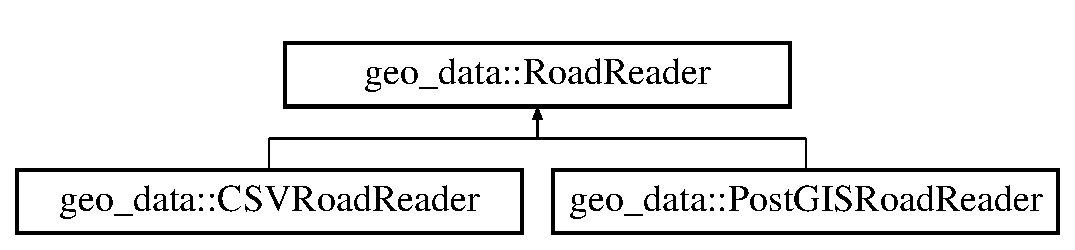
\includegraphics[height=2.000000cm]{classgeo__data_1_1RoadReader}
\end{center}
\end{figure}
\subsection*{Public Types}
\begin{DoxyCompactItemize}
\item 
using {\bfseries Ptr} = std\+::shared\+\_\+ptr$<$ \hyperlink{classgeo__data_1_1RoadReader}{Road\+Reader} $>$\hypertarget{classgeo__data_1_1RoadReader_a7f77731899e1a9d738bb07a7ee9bcceb}{}\label{classgeo__data_1_1RoadReader_a7f77731899e1a9d738bb07a7ee9bcceb}

\end{DoxyCompactItemize}
\subsection*{Public Member Functions}
\begin{DoxyCompactItemize}
\item 
virtual geo\+::\+Road\+::\+Ptr {\bfseries next\+\_\+road} (void)=0\hypertarget{classgeo__data_1_1RoadReader_a94d9bfa3df5ed6a7cfde3b765c5c330f}{}\label{classgeo__data_1_1RoadReader_a94d9bfa3df5ed6a7cfde3b765c5c330f}

\end{DoxyCompactItemize}


\subsection{Detailed Description}
Base class for reading \hyperlink{classgeo_1_1Road}{geo\+::\+Road} O\+SM road networks. 

The documentation for this class was generated from the following file\+:\begin{DoxyCompactItemize}
\item 
cvdi-\/src/geo-\/data/include/geo\+\_\+data.\+hpp\end{DoxyCompactItemize}

\hypertarget{classhmm__mm_1_1Router}{}\section{hmm\+\_\+mm\+:\+:Router Class Reference}
\label{classhmm__mm_1_1Router}\index{hmm\+\_\+mm\+::\+Router@{hmm\+\_\+mm\+::\+Router}}


Static class for find the lowest cost (shortest time) path between two sequential samples in the Hidden Markov Model.  




{\ttfamily \#include $<$hmm\+\_\+mm.\+hpp$>$}

\subsection*{Public Types}
\begin{DoxyCompactItemize}
\item 
using {\bfseries Target\+Road\+Point\+Map} = std\+::unordered\+\_\+map$<$ Road\+Point\+::\+Ptr, geo\+::\+Edge\+List\+Ptr $>$\hypertarget{classhmm__mm_1_1Router_a99494bcfdee07e82daa24fe929c17a4b}{}\label{classhmm__mm_1_1Router_a99494bcfdee07e82daa24fe929c17a4b}

\end{DoxyCompactItemize}
\subsection*{Static Public Member Functions}
\begin{DoxyCompactItemize}
\item 
static void \hyperlink{classhmm__mm_1_1Router_ade72964f9d0c24520f76757cde903d5f}{route} (Road\+Point\+::\+Ptr source, const Road\+Point\+Set \&targets, double max, Target\+Road\+Point\+Map \&out)\hypertarget{classhmm__mm_1_1Router_ade72964f9d0c24520f76757cde903d5f}{}\label{classhmm__mm_1_1Router_ade72964f9d0c24520f76757cde903d5f}

\begin{DoxyCompactList}\small\item\em Djikstra\textquotesingle{}s. \end{DoxyCompactList}\item 
static double {\bfseries time\+\_\+cost} (geo\+::\+Edge\+::\+Ptr edge)\hypertarget{classhmm__mm_1_1Router_ab7e4e5cdcd1b5a327c07966c8da6ae39}{}\label{classhmm__mm_1_1Router_ab7e4e5cdcd1b5a327c07966c8da6ae39}

\item 
static double {\bfseries time\+\_\+cost} (geo\+::\+Edge\+::\+Ptr edge, double fraction)\hypertarget{classhmm__mm_1_1Router_a2662b5cff27c1e0011ba8d09cbaea5d4}{}\label{classhmm__mm_1_1Router_a2662b5cff27c1e0011ba8d09cbaea5d4}

\item 
static double \hyperlink{classhmm__mm_1_1Router_a087113186f15df2c7c462a45d5569325}{route\+\_\+cost} (Road\+Point\+::\+Ptr start, Road\+Point\+::\+Ptr end, geo\+::\+Edge\+List \&path)\hypertarget{classhmm__mm_1_1Router_a087113186f15df2c7c462a45d5569325}{}\label{classhmm__mm_1_1Router_a087113186f15df2c7c462a45d5569325}

\begin{DoxyCompactList}\small\item\em Get the cost of a route in shortes time. \end{DoxyCompactList}\end{DoxyCompactItemize}
\subsection*{Static Public Attributes}
\begin{DoxyCompactItemize}
\item 
static constexpr float {\bfseries k\+Heuristic\+Speed} = 130.\+0\hypertarget{classhmm__mm_1_1Router_a28e87285dc841453be29c6ba6c27321c}{}\label{classhmm__mm_1_1Router_a28e87285dc841453be29c6ba6c27321c}

\item 
static constexpr double {\bfseries k\+Heuristic\+Priority} = 1.\+0\hypertarget{classhmm__mm_1_1Router_ae03d10c778bceb74cef64aca2c7c19cd}{}\label{classhmm__mm_1_1Router_ae03d10c778bceb74cef64aca2c7c19cd}

\end{DoxyCompactItemize}


\subsection{Detailed Description}
Static class for find the lowest cost (shortest time) path between two sequential samples in the Hidden Markov Model. 

The documentation for this class was generated from the following files\+:\begin{DoxyCompactItemize}
\item 
cvdi-\/src/hmm-\/mm/include/hmm\+\_\+mm.\+hpp\item 
cvdi-\/src/hmm-\/mm/src/hmm\+\_\+mm.\+cpp\end{DoxyCompactItemize}

\hypertarget{classfmt_1_1internal_1_1RuntimeError}{}\section{fmt\+:\+:internal\+:\+:Runtime\+Error Class Reference}
\label{classfmt_1_1internal_1_1RuntimeError}\index{fmt\+::internal\+::\+Runtime\+Error@{fmt\+::internal\+::\+Runtime\+Error}}
Inheritance diagram for fmt\+:\+:internal\+:\+:Runtime\+Error\+:\begin{figure}[H]
\begin{center}
\leavevmode
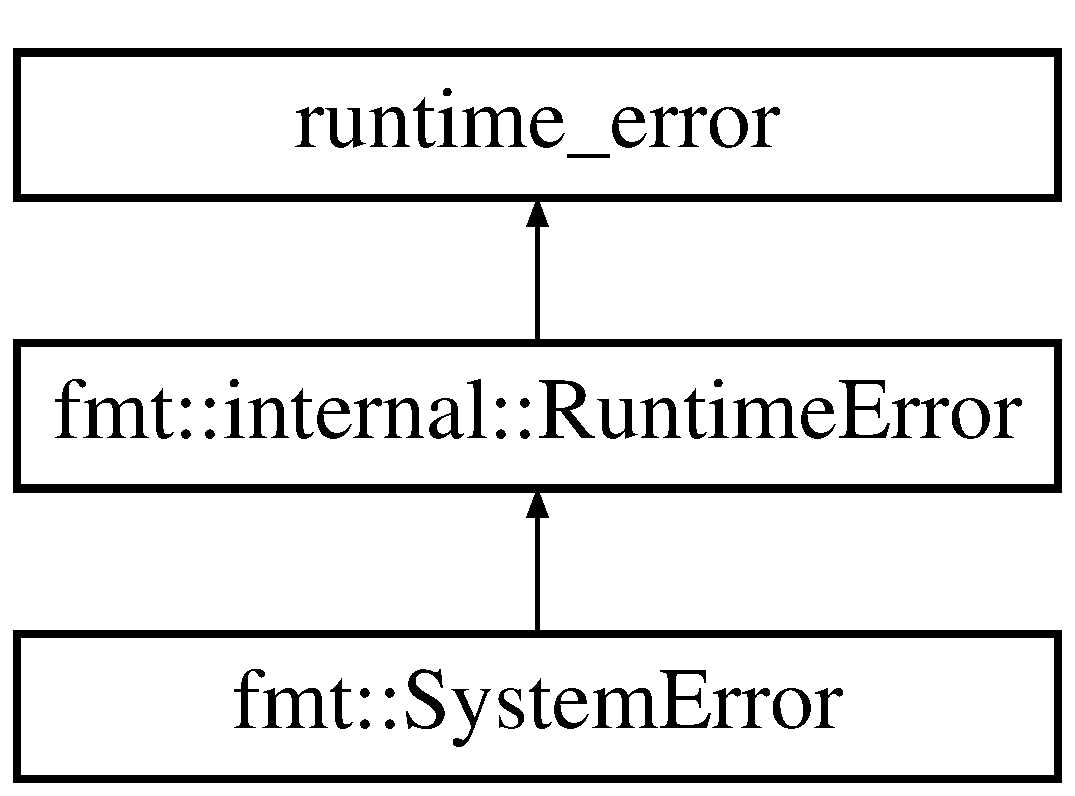
\includegraphics[height=3.000000cm]{classfmt_1_1internal_1_1RuntimeError}
\end{center}
\end{figure}


The documentation for this class was generated from the following files\+:\begin{DoxyCompactItemize}
\item 
cvdi-\/src/cvdi-\/cl/include/spdlog/fmt/bundled/format.\+h\item 
cvdi-\/src/cvdi-\/cl/include/spdlog/fmt/bundled/format.\+cc\end{DoxyCompactItemize}

\hypertarget{classgeo__data_1_1Sample}{}\section{geo\+\_\+data\+:\+:Sample Class Reference}
\label{classgeo__data_1_1Sample}\index{geo\+\_\+data\+::\+Sample@{geo\+\_\+data\+::\+Sample}}


{\ttfamily \#include $<$geo\+\_\+data.\+hpp$>$}

\subsection*{Public Types}
\begin{DoxyCompactItemize}
\item 
using {\bfseries Ptr} = std\+::shared\+\_\+ptr$<$ \hyperlink{classgeo__data_1_1Sample}{Sample} $>$\hypertarget{classgeo__data_1_1Sample_adf7988c796ed7425dff198fbb3556fcc}{}\label{classgeo__data_1_1Sample_adf7988c796ed7425dff198fbb3556fcc}

\item 
using {\bfseries Trace} = std\+::vector$<$ Ptr $>$\hypertarget{classgeo__data_1_1Sample_a6dedccb71de46de1b2ad54227962c3d7}{}\label{classgeo__data_1_1Sample_a6dedccb71de46de1b2ad54227962c3d7}

\end{DoxyCompactItemize}
\subsection*{Public Member Functions}
\begin{DoxyCompactItemize}
\item 
\hyperlink{classgeo__data_1_1Sample_a8d91847711c56badc1bce86f85ef23e4}{Sample} (const std\+::string \&\hyperlink{classgeo__data_1_1Sample_aa529b9aef77c02620eac7a5ada4adcb3}{id}, std\+::size\+\_\+t \hyperlink{classgeo__data_1_1Sample_a68267127a7cb00839ec904fcc0b9f64b}{index}, long \hyperlink{classgeo__data_1_1Sample_a7c6cd5157117296b306f8e5726737090}{timestamp}, double \hyperlink{classgeo__data_1_1Sample_a89ad23a22a5043e61e08129783333e4c}{lat}, double \hyperlink{classgeo__data_1_1Sample_a0f3322502b9f32fbc51462e4b6270381}{lon}, double \hyperlink{classgeo__data_1_1Sample_a9be314cd78a47730551e6169748edc96}{azimuth}, double \hyperlink{classgeo__data_1_1Sample_a77437a286640779148c3f4905b90a16c}{speed}, const std\+::string \&\hyperlink{classgeo__data_1_1Sample_ac7ebb4bddcc448ab65843f29f7e3d2a5}{record}, bool \hyperlink{classgeo__data_1_1Sample_ae009ad7cc3106219b77123ba4e5d3238}{is\+\_\+valid}=true, \hyperlink{namespacegeo__data_a2374ba83ef1f8bcad5d82c67dc7c8ddd}{Sample\+Error} \hyperlink{classgeo__data_1_1Sample_a6aaf864d36093ef23cb5a273d45f4f01}{error\+\_\+type}=Sample\+Error\+::\+N\+O\+NE, const std\+::string \&\hyperlink{classgeo__data_1_1Sample_a5ad107d3bca8ca053e785f24efae6c28}{error\+\_\+msg}=\char`\"{}\char`\"{})
\begin{DoxyCompactList}\small\item\em Construct a \hyperlink{classgeo__data_1_1Sample}{Sample} object. A sample is valid if it was created successfully from the C\+SV record. Invalid records have missing fields, invalid G\+PS, or values that are not able to be converted to the required type. \end{DoxyCompactList}\item 
std\+::string \hyperlink{classgeo__data_1_1Sample_aa529b9aef77c02620eac7a5ada4adcb3}{id} () const 
\begin{DoxyCompactList}\small\item\em Get the ID of this sample. \end{DoxyCompactList}\item 
std\+::size\+\_\+t \hyperlink{classgeo__data_1_1Sample_a68267127a7cb00839ec904fcc0b9f64b}{index} () const 
\begin{DoxyCompactList}\small\item\em Get the index of this sample in the trace. Because sample\textquotesingle{}s can be re-\/indexed due to errors and filtering, this might differ from the sample\textquotesingle{}s index in the C\+SV file. \end{DoxyCompactList}\item 
std\+::size\+\_\+t \hyperlink{classgeo__data_1_1Sample_ac7ed68fe4f3e48e77a43ba52be3838e9}{raw\+\_\+index} () const 
\begin{DoxyCompactList}\small\item\em Get the raw index of this sample in the trace. The raw index is the initial index of sample in the C\+SV file, irrespective of the filtering or errors. \end{DoxyCompactList}\item 
long \hyperlink{classgeo__data_1_1Sample_a7c6cd5157117296b306f8e5726737090}{timestamp} () const 
\begin{DoxyCompactList}\small\item\em Get the Unix timestamp of this sample in seconds. \end{DoxyCompactList}\item 
double \hyperlink{classgeo__data_1_1Sample_a89ad23a22a5043e61e08129783333e4c}{lat} () const 
\begin{DoxyCompactList}\small\item\em Get the G\+PS latitude of this sample in decimal degrees. \end{DoxyCompactList}\item 
double \hyperlink{classgeo__data_1_1Sample_a0f3322502b9f32fbc51462e4b6270381}{lon} () const 
\begin{DoxyCompactList}\small\item\em Get the G\+PS of this sample in decimal degrees. \end{DoxyCompactList}\item 
double \hyperlink{classgeo__data_1_1Sample_a9be314cd78a47730551e6169748edc96}{azimuth} () const 
\begin{DoxyCompactList}\small\item\em Get azimuth (header or bearing) in degrees from north of the sample. \end{DoxyCompactList}\item 
double \hyperlink{classgeo__data_1_1Sample_a77437a286640779148c3f4905b90a16c}{speed} () const 
\begin{DoxyCompactList}\small\item\em Get the speed in meters per second of the sample. \end{DoxyCompactList}\item 
std\+::string \hyperlink{classgeo__data_1_1Sample_ac7ebb4bddcc448ab65843f29f7e3d2a5}{record} () const 
\begin{DoxyCompactList}\small\item\em Get the underlying C\+SV record for this sample. \end{DoxyCompactList}\item 
bool \hyperlink{classgeo__data_1_1Sample_ae009ad7cc3106219b77123ba4e5d3238}{is\+\_\+valid} () const 
\begin{DoxyCompactList}\small\item\em Return true if sample is valid. A sample is valid if it was created successfully from the C\+SV record. Invalid records have missing fields, invalid G\+PS, or values that are not convertible to the required type. \end{DoxyCompactList}\item 
\hyperlink{namespacegeo__data_a2374ba83ef1f8bcad5d82c67dc7c8ddd}{Sample\+Error} \hyperlink{classgeo__data_1_1Sample_a6aaf864d36093ef23cb5a273d45f4f01}{error\+\_\+type} () const 
\begin{DoxyCompactList}\small\item\em Get the Sample\+Error type for the sample. \end{DoxyCompactList}\item 
std\+::string \hyperlink{classgeo__data_1_1Sample_a5ad107d3bca8ca053e785f24efae6c28}{error\+\_\+msg} () const 
\begin{DoxyCompactList}\small\item\em Get the error message of the sample. \end{DoxyCompactList}\item 
geo\+::\+Edge\+::\+Ptr \hyperlink{classgeo__data_1_1Sample_a17881dc1186aa58c6923187b4386bf45}{matched\+\_\+edge} () const 
\begin{DoxyCompactList}\small\item\em Get the matched edge for the sample. \end{DoxyCompactList}\item 
geo\+::\+Edge\+::\+Ptr \hyperlink{classgeo__data_1_1Sample_adf2425e64a0cda4f6f247ec89ee9f708}{fit\+\_\+edge} () const 
\begin{DoxyCompactList}\small\item\em Get the fit edge for the sample. \end{DoxyCompactList}\item 
bool \hyperlink{classgeo__data_1_1Sample_a2c71fa2fbc417fcb031da4009d15c4ea}{is\+\_\+explicit\+\_\+fit} () const 
\begin{DoxyCompactList}\small\item\em Return true if this sample is map matched and falls within the area of the mapped edge. \end{DoxyCompactList}\item 
Interval\+::\+Ptr \hyperlink{classgeo__data_1_1Sample_a4461eedbc44d2a528f2e502929bb1053}{interval} () const 
\begin{DoxyCompactList}\small\item\em Get the interval (critical or private) of this sample. \end{DoxyCompactList}\item 
uint32\+\_\+t \hyperlink{classgeo__data_1_1Sample_aee00b5ede8ede7cb8119c4a94f85fe8e}{out\+\_\+degree} () const 
\begin{DoxyCompactList}\small\item\em Get the cumulative trace out degree of the trace at this sample. \end{DoxyCompactList}\item 
void \hyperlink{classgeo__data_1_1Sample_a9e2a4ac09187e72f582122253531c669}{matched\+\_\+edge} (geo\+::\+Edge\+::\+Ptr edge)
\begin{DoxyCompactList}\small\item\em Set the matched edge of this sample. \end{DoxyCompactList}\item 
void \hyperlink{classgeo__data_1_1Sample_ad968e18e8b77a4325e1245f2333d802e}{fit\+\_\+edge} (geo\+::\+Edge\+::\+Ptr edge)
\begin{DoxyCompactList}\small\item\em Set the fit edge of this sample. \end{DoxyCompactList}\item 
void \hyperlink{classgeo__data_1_1Sample_abc387126ac2a9285599aa7b4d243cdb5}{is\+\_\+explicit\+\_\+fit} (bool explicit\+\_\+fit)
\begin{DoxyCompactList}\small\item\em Set the sample to be explicitly fit. \end{DoxyCompactList}\item 
void \hyperlink{classgeo__data_1_1Sample_a7c69af72f22c276d96ac9b17d5a5b250}{interval} (Interval\+::\+Ptr interval)
\begin{DoxyCompactList}\small\item\em Set the interval (private or critical) for the sample. \end{DoxyCompactList}\item 
void \hyperlink{classgeo__data_1_1Sample_ad339548ab91c90be41c9be2c81d3d07a}{out\+\_\+degree} (uint32\+\_\+t out\+\_\+degree)
\begin{DoxyCompactList}\small\item\em Set the cumulative trace out degree of the sample. \end{DoxyCompactList}\item 
void \hyperlink{classgeo__data_1_1Sample_af432c7b67cb2280eaac5d0d8c24163bf}{index} (std\+::size\+\_\+t index)
\begin{DoxyCompactList}\small\item\em Set the index of the sample. \end{DoxyCompactList}\end{DoxyCompactItemize}
\subsection*{Public Attributes}
\begin{DoxyCompactItemize}
\item 
O\+G\+R\+Point \hyperlink{classgeo__data_1_1Sample_abb1a8679c0f245bc614b7f5168af3f8d}{point}\hypertarget{classgeo__data_1_1Sample_abb1a8679c0f245bc614b7f5168af3f8d}{}\label{classgeo__data_1_1Sample_abb1a8679c0f245bc614b7f5168af3f8d}

\begin{DoxyCompactList}\small\item\em The underlying O\+G\+R\+Point for the G\+PS coordinates of the sample. \end{DoxyCompactList}\end{DoxyCompactItemize}


\subsection{Detailed Description}
B\+S\+M\+P1 connected vehicle trace \hyperlink{classgeo__data_1_1Sample}{Sample} object. Samples represent a spatial-\/temporal point created by an on-\/board device. Samples are part of a G\+PS sequence trace, which represents a self contained vehicle trajectory. The underlying G\+PS point is contained within an O\+G\+R\+Point object.

The record for a sample is a C\+SV line. The record must have the correct format, number of fields, and unit types. Although only a few fields are used in the sample, the entire record must be correct to avoid flagging the record (and sample) as invalid. Invalid records have missing fields, invalid G\+PS, or values that are not convertible to the required type.

Samples have associated road edges. There are two types these edges, matched and fit. A matched edge is the edge to which the sample is map matched. A fit edge is edge to which the sample\textquotesingle{}s G\+PS point falls within the \hyperlink{classgeo_1_1Area}{geo\+::\+Area} of the edge. If a sample has a matched edge and falls with the area of that edge, then that edge is also the sample\textquotesingle{}s fit edge. If the sample does not have a matched edge or does not fall within the area of its matched edge, then the sample will have an implicit fit edge.

Samples have associated intervals marking the sample as critical or private.

Samples also store the accumulated out degree of the trace. This will be zero at the beginning of the trace and the maximum out degree at the end of the trace. 

\subsection{Constructor \& Destructor Documentation}
\index{geo\+\_\+data\+::\+Sample@{geo\+\_\+data\+::\+Sample}!Sample@{Sample}}
\index{Sample@{Sample}!geo\+\_\+data\+::\+Sample@{geo\+\_\+data\+::\+Sample}}
\subsubsection[{\texorpdfstring{Sample(const std\+::string \&id, std\+::size\+\_\+t index, long timestamp, double lat, double lon, double azimuth, double speed, const std\+::string \&record, bool is\+\_\+valid=true, Sample\+Error error\+\_\+type=\+Sample\+Error\+::\+N\+O\+N\+E, const std\+::string \&error\+\_\+msg="""")}{Sample(const std::string &id, std::size_t index, long timestamp, double lat, double lon, double azimuth, double speed, const std::string &record, bool is_valid=true, SampleError error_type=SampleError::NONE, const std::string &error_msg="")}}]{\setlength{\rightskip}{0pt plus 5cm}geo\+\_\+data\+::\+Sample\+::\+Sample (
\begin{DoxyParamCaption}
\item[{const std\+::string \&}]{id, }
\item[{std\+::size\+\_\+t}]{index, }
\item[{long}]{timestamp, }
\item[{double}]{lat, }
\item[{double}]{lon, }
\item[{double}]{azimuth, }
\item[{double}]{speed, }
\item[{const std\+::string \&}]{record, }
\item[{bool}]{is\+\_\+valid = {\ttfamily true}, }
\item[{{\bf Sample\+Error}}]{error\+\_\+type = {\ttfamily SampleError\+:\+:NONE}, }
\item[{const std\+::string \&}]{error\+\_\+msg = {\ttfamily \char`\"{}\char`\"{}}}
\end{DoxyParamCaption}
)}\hypertarget{classgeo__data_1_1Sample_a8d91847711c56badc1bce86f85ef23e4}{}\label{classgeo__data_1_1Sample_a8d91847711c56badc1bce86f85ef23e4}


Construct a \hyperlink{classgeo__data_1_1Sample}{Sample} object. A sample is valid if it was created successfully from the C\+SV record. Invalid records have missing fields, invalid G\+PS, or values that are not able to be converted to the required type. 


\begin{DoxyParams}{Parameters}
{\em id} & unique ID of this sample \\
\hline
{\em index} & index of this sample within the trace \\
\hline
{\em timestamp} & Unix timestamp as seconds \\
\hline
{\em lat} & the decimal G\+PS latitude of the sample \\
\hline
{\em lon} & the decimal G\+PS longitude of the sample \\
\hline
{\em azimuth} & the azimuth (heading or bearing) in degrees from north \\
\hline
{\em speed} & the instantaneous velocity in meters per second of the vehicle for this sample \\
\hline
{\em record} & the raw C\+SV record for this sample \\
\hline
{\em is\+\_\+valid} & flag indicating the sample is valid \\
\hline
{\em error\+\_\+type} & indicates Sample\+Error type of the sample \\
\hline
{\em error\+\_\+msg} & message for the sample \\
\hline
\end{DoxyParams}


\subsection{Member Function Documentation}
\index{geo\+\_\+data\+::\+Sample@{geo\+\_\+data\+::\+Sample}!azimuth@{azimuth}}
\index{azimuth@{azimuth}!geo\+\_\+data\+::\+Sample@{geo\+\_\+data\+::\+Sample}}
\subsubsection[{\texorpdfstring{azimuth() const }{azimuth() const }}]{\setlength{\rightskip}{0pt plus 5cm}double geo\+\_\+data\+::\+Sample\+::azimuth (
\begin{DoxyParamCaption}
{}
\end{DoxyParamCaption}
) const}\hypertarget{classgeo__data_1_1Sample_a9be314cd78a47730551e6169748edc96}{}\label{classgeo__data_1_1Sample_a9be314cd78a47730551e6169748edc96}


Get azimuth (header or bearing) in degrees from north of the sample. 

\begin{DoxyReturn}{Returns}
the azimuth 
\end{DoxyReturn}
\index{geo\+\_\+data\+::\+Sample@{geo\+\_\+data\+::\+Sample}!error\+\_\+msg@{error\+\_\+msg}}
\index{error\+\_\+msg@{error\+\_\+msg}!geo\+\_\+data\+::\+Sample@{geo\+\_\+data\+::\+Sample}}
\subsubsection[{\texorpdfstring{error\+\_\+msg() const }{error_msg() const }}]{\setlength{\rightskip}{0pt plus 5cm}std\+::string geo\+\_\+data\+::\+Sample\+::error\+\_\+msg (
\begin{DoxyParamCaption}
{}
\end{DoxyParamCaption}
) const}\hypertarget{classgeo__data_1_1Sample_a5ad107d3bca8ca053e785f24efae6c28}{}\label{classgeo__data_1_1Sample_a5ad107d3bca8ca053e785f24efae6c28}


Get the error message of the sample. 

\begin{DoxyReturn}{Returns}
the error message 
\end{DoxyReturn}
\index{geo\+\_\+data\+::\+Sample@{geo\+\_\+data\+::\+Sample}!error\+\_\+type@{error\+\_\+type}}
\index{error\+\_\+type@{error\+\_\+type}!geo\+\_\+data\+::\+Sample@{geo\+\_\+data\+::\+Sample}}
\subsubsection[{\texorpdfstring{error\+\_\+type() const }{error_type() const }}]{\setlength{\rightskip}{0pt plus 5cm}{\bf Sample\+Error} geo\+\_\+data\+::\+Sample\+::error\+\_\+type (
\begin{DoxyParamCaption}
{}
\end{DoxyParamCaption}
) const}\hypertarget{classgeo__data_1_1Sample_a6aaf864d36093ef23cb5a273d45f4f01}{}\label{classgeo__data_1_1Sample_a6aaf864d36093ef23cb5a273d45f4f01}


Get the Sample\+Error type for the sample. 

\begin{DoxyReturn}{Returns}
the sample error type 
\end{DoxyReturn}
\index{geo\+\_\+data\+::\+Sample@{geo\+\_\+data\+::\+Sample}!fit\+\_\+edge@{fit\+\_\+edge}}
\index{fit\+\_\+edge@{fit\+\_\+edge}!geo\+\_\+data\+::\+Sample@{geo\+\_\+data\+::\+Sample}}
\subsubsection[{\texorpdfstring{fit\+\_\+edge() const }{fit_edge() const }}]{\setlength{\rightskip}{0pt plus 5cm}geo\+::\+Edge\+::\+Ptr geo\+\_\+data\+::\+Sample\+::fit\+\_\+edge (
\begin{DoxyParamCaption}
{}
\end{DoxyParamCaption}
) const}\hypertarget{classgeo__data_1_1Sample_adf2425e64a0cda4f6f247ec89ee9f708}{}\label{classgeo__data_1_1Sample_adf2425e64a0cda4f6f247ec89ee9f708}


Get the fit edge for the sample. 

\begin{DoxyReturn}{Returns}
a pointer to the fit edge 
\end{DoxyReturn}
\index{geo\+\_\+data\+::\+Sample@{geo\+\_\+data\+::\+Sample}!fit\+\_\+edge@{fit\+\_\+edge}}
\index{fit\+\_\+edge@{fit\+\_\+edge}!geo\+\_\+data\+::\+Sample@{geo\+\_\+data\+::\+Sample}}
\subsubsection[{\texorpdfstring{fit\+\_\+edge(geo\+::\+Edge\+::\+Ptr edge)}{fit_edge(geo::Edge::Ptr edge)}}]{\setlength{\rightskip}{0pt plus 5cm}void geo\+\_\+data\+::\+Sample\+::fit\+\_\+edge (
\begin{DoxyParamCaption}
\item[{geo\+::\+Edge\+::\+Ptr}]{edge}
\end{DoxyParamCaption}
)}\hypertarget{classgeo__data_1_1Sample_ad968e18e8b77a4325e1245f2333d802e}{}\label{classgeo__data_1_1Sample_ad968e18e8b77a4325e1245f2333d802e}


Set the fit edge of this sample. 


\begin{DoxyParams}{Parameters}
{\em pointer} & to the fit edge \\
\hline
\end{DoxyParams}
\index{geo\+\_\+data\+::\+Sample@{geo\+\_\+data\+::\+Sample}!id@{id}}
\index{id@{id}!geo\+\_\+data\+::\+Sample@{geo\+\_\+data\+::\+Sample}}
\subsubsection[{\texorpdfstring{id() const }{id() const }}]{\setlength{\rightskip}{0pt plus 5cm}std\+::string geo\+\_\+data\+::\+Sample\+::id (
\begin{DoxyParamCaption}
{}
\end{DoxyParamCaption}
) const}\hypertarget{classgeo__data_1_1Sample_aa529b9aef77c02620eac7a5ada4adcb3}{}\label{classgeo__data_1_1Sample_aa529b9aef77c02620eac7a5ada4adcb3}


Get the ID of this sample. 

\begin{DoxyReturn}{Returns}
the ID 
\end{DoxyReturn}
\index{geo\+\_\+data\+::\+Sample@{geo\+\_\+data\+::\+Sample}!index@{index}}
\index{index@{index}!geo\+\_\+data\+::\+Sample@{geo\+\_\+data\+::\+Sample}}
\subsubsection[{\texorpdfstring{index() const }{index() const }}]{\setlength{\rightskip}{0pt plus 5cm}std\+::size\+\_\+t geo\+\_\+data\+::\+Sample\+::index (
\begin{DoxyParamCaption}
{}
\end{DoxyParamCaption}
) const}\hypertarget{classgeo__data_1_1Sample_a68267127a7cb00839ec904fcc0b9f64b}{}\label{classgeo__data_1_1Sample_a68267127a7cb00839ec904fcc0b9f64b}


Get the index of this sample in the trace. Because sample\textquotesingle{}s can be re-\/indexed due to errors and filtering, this might differ from the sample\textquotesingle{}s index in the C\+SV file. 

\begin{DoxyReturn}{Returns}
the index 
\end{DoxyReturn}
\index{geo\+\_\+data\+::\+Sample@{geo\+\_\+data\+::\+Sample}!index@{index}}
\index{index@{index}!geo\+\_\+data\+::\+Sample@{geo\+\_\+data\+::\+Sample}}
\subsubsection[{\texorpdfstring{index(std\+::size\+\_\+t index)}{index(std::size_t index)}}]{\setlength{\rightskip}{0pt plus 5cm}void geo\+\_\+data\+::\+Sample\+::index (
\begin{DoxyParamCaption}
\item[{std\+::size\+\_\+t}]{index}
\end{DoxyParamCaption}
)}\hypertarget{classgeo__data_1_1Sample_af432c7b67cb2280eaac5d0d8c24163bf}{}\label{classgeo__data_1_1Sample_af432c7b67cb2280eaac5d0d8c24163bf}


Set the index of the sample. 


\begin{DoxyParams}{Parameters}
{\em the} & new index of the sample \\
\hline
\end{DoxyParams}
\index{geo\+\_\+data\+::\+Sample@{geo\+\_\+data\+::\+Sample}!interval@{interval}}
\index{interval@{interval}!geo\+\_\+data\+::\+Sample@{geo\+\_\+data\+::\+Sample}}
\subsubsection[{\texorpdfstring{interval() const }{interval() const }}]{\setlength{\rightskip}{0pt plus 5cm}Interval\+::\+Ptr geo\+\_\+data\+::\+Sample\+::interval (
\begin{DoxyParamCaption}
{}
\end{DoxyParamCaption}
) const}\hypertarget{classgeo__data_1_1Sample_a4461eedbc44d2a528f2e502929bb1053}{}\label{classgeo__data_1_1Sample_a4461eedbc44d2a528f2e502929bb1053}


Get the interval (critical or private) of this sample. 

\begin{DoxyReturn}{Returns}
a pointer to the interval 
\end{DoxyReturn}
\index{geo\+\_\+data\+::\+Sample@{geo\+\_\+data\+::\+Sample}!interval@{interval}}
\index{interval@{interval}!geo\+\_\+data\+::\+Sample@{geo\+\_\+data\+::\+Sample}}
\subsubsection[{\texorpdfstring{interval(\+Interval\+::\+Ptr interval)}{interval(Interval::Ptr interval)}}]{\setlength{\rightskip}{0pt plus 5cm}void geo\+\_\+data\+::\+Sample\+::interval (
\begin{DoxyParamCaption}
\item[{Interval\+::\+Ptr}]{interval}
\end{DoxyParamCaption}
)}\hypertarget{classgeo__data_1_1Sample_a7c69af72f22c276d96ac9b17d5a5b250}{}\label{classgeo__data_1_1Sample_a7c69af72f22c276d96ac9b17d5a5b250}


Set the interval (private or critical) for the sample. 


\begin{DoxyParams}{Parameters}
{\em pointer} & the interval \\
\hline
\end{DoxyParams}
\index{geo\+\_\+data\+::\+Sample@{geo\+\_\+data\+::\+Sample}!is\+\_\+explicit\+\_\+fit@{is\+\_\+explicit\+\_\+fit}}
\index{is\+\_\+explicit\+\_\+fit@{is\+\_\+explicit\+\_\+fit}!geo\+\_\+data\+::\+Sample@{geo\+\_\+data\+::\+Sample}}
\subsubsection[{\texorpdfstring{is\+\_\+explicit\+\_\+fit() const }{is_explicit_fit() const }}]{\setlength{\rightskip}{0pt plus 5cm}bool geo\+\_\+data\+::\+Sample\+::is\+\_\+explicit\+\_\+fit (
\begin{DoxyParamCaption}
{}
\end{DoxyParamCaption}
) const}\hypertarget{classgeo__data_1_1Sample_a2c71fa2fbc417fcb031da4009d15c4ea}{}\label{classgeo__data_1_1Sample_a2c71fa2fbc417fcb031da4009d15c4ea}


Return true if this sample is map matched and falls within the area of the mapped edge. 

\begin{DoxyReturn}{Returns}
true if explicitly fit, false otherwise 
\end{DoxyReturn}
\index{geo\+\_\+data\+::\+Sample@{geo\+\_\+data\+::\+Sample}!is\+\_\+explicit\+\_\+fit@{is\+\_\+explicit\+\_\+fit}}
\index{is\+\_\+explicit\+\_\+fit@{is\+\_\+explicit\+\_\+fit}!geo\+\_\+data\+::\+Sample@{geo\+\_\+data\+::\+Sample}}
\subsubsection[{\texorpdfstring{is\+\_\+explicit\+\_\+fit(bool explicit\+\_\+fit)}{is_explicit_fit(bool explicit_fit)}}]{\setlength{\rightskip}{0pt plus 5cm}void geo\+\_\+data\+::\+Sample\+::is\+\_\+explicit\+\_\+fit (
\begin{DoxyParamCaption}
\item[{bool}]{explicit\+\_\+fit}
\end{DoxyParamCaption}
)}\hypertarget{classgeo__data_1_1Sample_abc387126ac2a9285599aa7b4d243cdb5}{}\label{classgeo__data_1_1Sample_abc387126ac2a9285599aa7b4d243cdb5}


Set the sample to be explicitly fit. 


\begin{DoxyParams}{Parameters}
{\em flag} & for explicitly fit \\
\hline
\end{DoxyParams}
\index{geo\+\_\+data\+::\+Sample@{geo\+\_\+data\+::\+Sample}!is\+\_\+valid@{is\+\_\+valid}}
\index{is\+\_\+valid@{is\+\_\+valid}!geo\+\_\+data\+::\+Sample@{geo\+\_\+data\+::\+Sample}}
\subsubsection[{\texorpdfstring{is\+\_\+valid() const }{is_valid() const }}]{\setlength{\rightskip}{0pt plus 5cm}bool geo\+\_\+data\+::\+Sample\+::is\+\_\+valid (
\begin{DoxyParamCaption}
{}
\end{DoxyParamCaption}
) const}\hypertarget{classgeo__data_1_1Sample_ae009ad7cc3106219b77123ba4e5d3238}{}\label{classgeo__data_1_1Sample_ae009ad7cc3106219b77123ba4e5d3238}


Return true if sample is valid. A sample is valid if it was created successfully from the C\+SV record. Invalid records have missing fields, invalid G\+PS, or values that are not convertible to the required type. 

\begin{DoxyReturn}{Returns}
true if the sample is valid, false otherwise 
\end{DoxyReturn}
\index{geo\+\_\+data\+::\+Sample@{geo\+\_\+data\+::\+Sample}!lat@{lat}}
\index{lat@{lat}!geo\+\_\+data\+::\+Sample@{geo\+\_\+data\+::\+Sample}}
\subsubsection[{\texorpdfstring{lat() const }{lat() const }}]{\setlength{\rightskip}{0pt plus 5cm}double geo\+\_\+data\+::\+Sample\+::lat (
\begin{DoxyParamCaption}
{}
\end{DoxyParamCaption}
) const}\hypertarget{classgeo__data_1_1Sample_a89ad23a22a5043e61e08129783333e4c}{}\label{classgeo__data_1_1Sample_a89ad23a22a5043e61e08129783333e4c}


Get the G\+PS latitude of this sample in decimal degrees. 

\begin{DoxyReturn}{Returns}
the latitude 
\end{DoxyReturn}
\index{geo\+\_\+data\+::\+Sample@{geo\+\_\+data\+::\+Sample}!lon@{lon}}
\index{lon@{lon}!geo\+\_\+data\+::\+Sample@{geo\+\_\+data\+::\+Sample}}
\subsubsection[{\texorpdfstring{lon() const }{lon() const }}]{\setlength{\rightskip}{0pt plus 5cm}double geo\+\_\+data\+::\+Sample\+::lon (
\begin{DoxyParamCaption}
{}
\end{DoxyParamCaption}
) const}\hypertarget{classgeo__data_1_1Sample_a0f3322502b9f32fbc51462e4b6270381}{}\label{classgeo__data_1_1Sample_a0f3322502b9f32fbc51462e4b6270381}


Get the G\+PS of this sample in decimal degrees. 

\begin{DoxyReturn}{Returns}
the longitude 
\end{DoxyReturn}
\index{geo\+\_\+data\+::\+Sample@{geo\+\_\+data\+::\+Sample}!matched\+\_\+edge@{matched\+\_\+edge}}
\index{matched\+\_\+edge@{matched\+\_\+edge}!geo\+\_\+data\+::\+Sample@{geo\+\_\+data\+::\+Sample}}
\subsubsection[{\texorpdfstring{matched\+\_\+edge() const }{matched_edge() const }}]{\setlength{\rightskip}{0pt plus 5cm}geo\+::\+Edge\+::\+Ptr geo\+\_\+data\+::\+Sample\+::matched\+\_\+edge (
\begin{DoxyParamCaption}
{}
\end{DoxyParamCaption}
) const}\hypertarget{classgeo__data_1_1Sample_a17881dc1186aa58c6923187b4386bf45}{}\label{classgeo__data_1_1Sample_a17881dc1186aa58c6923187b4386bf45}


Get the matched edge for the sample. 

\begin{DoxyReturn}{Returns}
a pointer the matched edge 
\end{DoxyReturn}
\index{geo\+\_\+data\+::\+Sample@{geo\+\_\+data\+::\+Sample}!matched\+\_\+edge@{matched\+\_\+edge}}
\index{matched\+\_\+edge@{matched\+\_\+edge}!geo\+\_\+data\+::\+Sample@{geo\+\_\+data\+::\+Sample}}
\subsubsection[{\texorpdfstring{matched\+\_\+edge(geo\+::\+Edge\+::\+Ptr edge)}{matched_edge(geo::Edge::Ptr edge)}}]{\setlength{\rightskip}{0pt plus 5cm}void geo\+\_\+data\+::\+Sample\+::matched\+\_\+edge (
\begin{DoxyParamCaption}
\item[{geo\+::\+Edge\+::\+Ptr}]{edge}
\end{DoxyParamCaption}
)}\hypertarget{classgeo__data_1_1Sample_a9e2a4ac09187e72f582122253531c669}{}\label{classgeo__data_1_1Sample_a9e2a4ac09187e72f582122253531c669}


Set the matched edge of this sample. 


\begin{DoxyParams}{Parameters}
{\em pointer} & to the matched edge \\
\hline
\end{DoxyParams}
\index{geo\+\_\+data\+::\+Sample@{geo\+\_\+data\+::\+Sample}!out\+\_\+degree@{out\+\_\+degree}}
\index{out\+\_\+degree@{out\+\_\+degree}!geo\+\_\+data\+::\+Sample@{geo\+\_\+data\+::\+Sample}}
\subsubsection[{\texorpdfstring{out\+\_\+degree() const }{out_degree() const }}]{\setlength{\rightskip}{0pt plus 5cm}uint32\+\_\+t geo\+\_\+data\+::\+Sample\+::out\+\_\+degree (
\begin{DoxyParamCaption}
{}
\end{DoxyParamCaption}
) const}\hypertarget{classgeo__data_1_1Sample_aee00b5ede8ede7cb8119c4a94f85fe8e}{}\label{classgeo__data_1_1Sample_aee00b5ede8ede7cb8119c4a94f85fe8e}


Get the cumulative trace out degree of the trace at this sample. 

\begin{DoxyReturn}{Returns}
the out degree 
\end{DoxyReturn}
\index{geo\+\_\+data\+::\+Sample@{geo\+\_\+data\+::\+Sample}!out\+\_\+degree@{out\+\_\+degree}}
\index{out\+\_\+degree@{out\+\_\+degree}!geo\+\_\+data\+::\+Sample@{geo\+\_\+data\+::\+Sample}}
\subsubsection[{\texorpdfstring{out\+\_\+degree(uint32\+\_\+t out\+\_\+degree)}{out_degree(uint32_t out_degree)}}]{\setlength{\rightskip}{0pt plus 5cm}void geo\+\_\+data\+::\+Sample\+::out\+\_\+degree (
\begin{DoxyParamCaption}
\item[{uint32\+\_\+t}]{out\+\_\+degree}
\end{DoxyParamCaption}
)}\hypertarget{classgeo__data_1_1Sample_ad339548ab91c90be41c9be2c81d3d07a}{}\label{classgeo__data_1_1Sample_ad339548ab91c90be41c9be2c81d3d07a}


Set the cumulative trace out degree of the sample. 


\begin{DoxyParams}{Parameters}
{\em the} & out degree \\
\hline
\end{DoxyParams}
\index{geo\+\_\+data\+::\+Sample@{geo\+\_\+data\+::\+Sample}!raw\+\_\+index@{raw\+\_\+index}}
\index{raw\+\_\+index@{raw\+\_\+index}!geo\+\_\+data\+::\+Sample@{geo\+\_\+data\+::\+Sample}}
\subsubsection[{\texorpdfstring{raw\+\_\+index() const }{raw_index() const }}]{\setlength{\rightskip}{0pt plus 5cm}std\+::size\+\_\+t geo\+\_\+data\+::\+Sample\+::raw\+\_\+index (
\begin{DoxyParamCaption}
{}
\end{DoxyParamCaption}
) const}\hypertarget{classgeo__data_1_1Sample_ac7ed68fe4f3e48e77a43ba52be3838e9}{}\label{classgeo__data_1_1Sample_ac7ed68fe4f3e48e77a43ba52be3838e9}


Get the raw index of this sample in the trace. The raw index is the initial index of sample in the C\+SV file, irrespective of the filtering or errors. 

\begin{DoxyReturn}{Returns}
the raw index 
\end{DoxyReturn}
\index{geo\+\_\+data\+::\+Sample@{geo\+\_\+data\+::\+Sample}!record@{record}}
\index{record@{record}!geo\+\_\+data\+::\+Sample@{geo\+\_\+data\+::\+Sample}}
\subsubsection[{\texorpdfstring{record() const }{record() const }}]{\setlength{\rightskip}{0pt plus 5cm}std\+::string geo\+\_\+data\+::\+Sample\+::record (
\begin{DoxyParamCaption}
{}
\end{DoxyParamCaption}
) const}\hypertarget{classgeo__data_1_1Sample_ac7ebb4bddcc448ab65843f29f7e3d2a5}{}\label{classgeo__data_1_1Sample_ac7ebb4bddcc448ab65843f29f7e3d2a5}


Get the underlying C\+SV record for this sample. 

\begin{DoxyReturn}{Returns}
the record 
\end{DoxyReturn}
\index{geo\+\_\+data\+::\+Sample@{geo\+\_\+data\+::\+Sample}!speed@{speed}}
\index{speed@{speed}!geo\+\_\+data\+::\+Sample@{geo\+\_\+data\+::\+Sample}}
\subsubsection[{\texorpdfstring{speed() const }{speed() const }}]{\setlength{\rightskip}{0pt plus 5cm}double geo\+\_\+data\+::\+Sample\+::speed (
\begin{DoxyParamCaption}
{}
\end{DoxyParamCaption}
) const}\hypertarget{classgeo__data_1_1Sample_a77437a286640779148c3f4905b90a16c}{}\label{classgeo__data_1_1Sample_a77437a286640779148c3f4905b90a16c}


Get the speed in meters per second of the sample. 

\begin{DoxyReturn}{Returns}
the speed 
\end{DoxyReturn}
\index{geo\+\_\+data\+::\+Sample@{geo\+\_\+data\+::\+Sample}!timestamp@{timestamp}}
\index{timestamp@{timestamp}!geo\+\_\+data\+::\+Sample@{geo\+\_\+data\+::\+Sample}}
\subsubsection[{\texorpdfstring{timestamp() const }{timestamp() const }}]{\setlength{\rightskip}{0pt plus 5cm}long geo\+\_\+data\+::\+Sample\+::timestamp (
\begin{DoxyParamCaption}
{}
\end{DoxyParamCaption}
) const}\hypertarget{classgeo__data_1_1Sample_a7c6cd5157117296b306f8e5726737090}{}\label{classgeo__data_1_1Sample_a7c6cd5157117296b306f8e5726737090}


Get the Unix timestamp of this sample in seconds. 

\begin{DoxyReturn}{Returns}
the timestamp 
\end{DoxyReturn}


The documentation for this class was generated from the following files\+:\begin{DoxyCompactItemize}
\item 
cvdi-\/src/geo-\/data/include/geo\+\_\+data.\+hpp\item 
cvdi-\/src/geo-\/data/src/geo\+\_\+data.\+cpp\end{DoxyCompactItemize}

\hypertarget{classMultiThread_1_1SharedQueue}{}\section{Multi\+Thread\+:\+:Shared\+Queue$<$ T $>$ Class Template Reference}
\label{classMultiThread_1_1SharedQueue}\index{Multi\+Thread\+::\+Shared\+Queue$<$ T $>$@{Multi\+Thread\+::\+Shared\+Queue$<$ T $>$}}
\subsection*{Public Member Functions}
\begin{DoxyCompactItemize}
\item 
T {\bfseries pop} ()\hypertarget{classMultiThread_1_1SharedQueue_a36f4fcdf32dfc9539cdb0f3063c6f23b}{}\label{classMultiThread_1_1SharedQueue_a36f4fcdf32dfc9539cdb0f3063c6f23b}

\item 
void {\bfseries pop} (T \&item)\hypertarget{classMultiThread_1_1SharedQueue_aa7c25303c0e03b7538c7c3943cdec3ae}{}\label{classMultiThread_1_1SharedQueue_aa7c25303c0e03b7538c7c3943cdec3ae}

\item 
void {\bfseries push} (const T \&item)\hypertarget{classMultiThread_1_1SharedQueue_a9679f3202c59d5cc645bb2dca4a40962}{}\label{classMultiThread_1_1SharedQueue_a9679f3202c59d5cc645bb2dca4a40962}

\item 
{\bfseries Shared\+Queue} (const \hyperlink{classMultiThread_1_1SharedQueue}{Shared\+Queue} \&)=delete\hypertarget{classMultiThread_1_1SharedQueue_ad93bc33944ebd48c36e68a04a406e8a7}{}\label{classMultiThread_1_1SharedQueue_ad93bc33944ebd48c36e68a04a406e8a7}

\item 
\hyperlink{classMultiThread_1_1SharedQueue}{Shared\+Queue} \& {\bfseries operator=} (const \hyperlink{classMultiThread_1_1SharedQueue}{Shared\+Queue} \&)=delete\hypertarget{classMultiThread_1_1SharedQueue_acda51e37bb05b2003fcfe69637dbbe3b}{}\label{classMultiThread_1_1SharedQueue_acda51e37bb05b2003fcfe69637dbbe3b}

\end{DoxyCompactItemize}


The documentation for this class was generated from the following file\+:\begin{DoxyCompactItemize}
\item 
cvdi-\/src/cvdi-\/cl/include/multi\+\_\+thread.\+hpp\end{DoxyCompactItemize}

\hypertarget{classspdlog_1_1details_1_1short__level__formatter}{}\section{spdlog\+:\+:details\+:\+:short\+\_\+level\+\_\+formatter Class Reference}
\label{classspdlog_1_1details_1_1short__level__formatter}\index{spdlog\+::details\+::short\+\_\+level\+\_\+formatter@{spdlog\+::details\+::short\+\_\+level\+\_\+formatter}}
Inheritance diagram for spdlog\+:\+:details\+:\+:short\+\_\+level\+\_\+formatter\+:\begin{figure}[H]
\begin{center}
\leavevmode
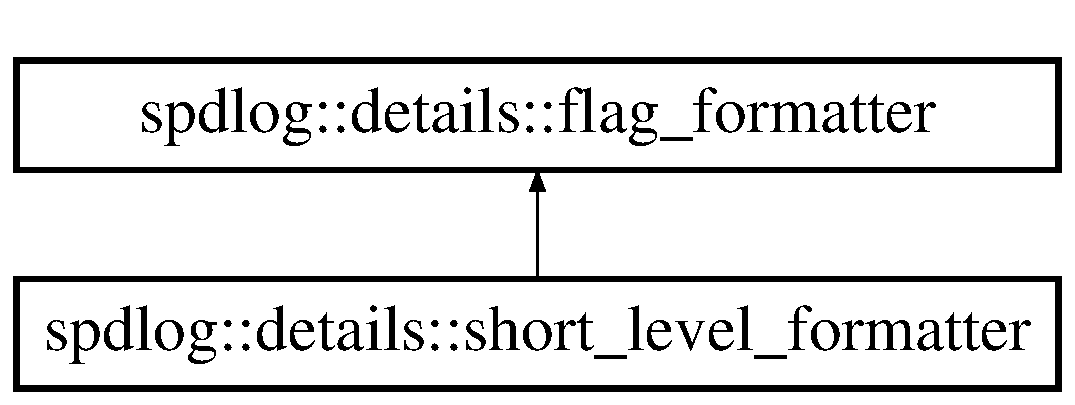
\includegraphics[height=2.000000cm]{classspdlog_1_1details_1_1short__level__formatter}
\end{center}
\end{figure}
\subsection*{Additional Inherited Members}


The documentation for this class was generated from the following file\+:\begin{DoxyCompactItemize}
\item 
cvdi-\/src/cvdi-\/cl/include/spdlog/details/pattern\+\_\+formatter\+\_\+impl.\+h\end{DoxyCompactItemize}

\hypertarget{structfmt_1_1internal_1_1SignChecker}{}\section{fmt\+:\+:internal\+:\+:Sign\+Checker$<$ Is\+Signed $>$ Struct Template Reference}
\label{structfmt_1_1internal_1_1SignChecker}\index{fmt\+::internal\+::\+Sign\+Checker$<$ Is\+Signed $>$@{fmt\+::internal\+::\+Sign\+Checker$<$ Is\+Signed $>$}}
\subsection*{Static Public Member Functions}
\begin{DoxyCompactItemize}
\item 
{\footnotesize template$<$typename T $>$ }\\static bool {\bfseries is\+\_\+negative} (T value)\hypertarget{structfmt_1_1internal_1_1SignChecker_ae60ea5795026fd1d83b34ec79d145baf}{}\label{structfmt_1_1internal_1_1SignChecker_ae60ea5795026fd1d83b34ec79d145baf}

\end{DoxyCompactItemize}


The documentation for this struct was generated from the following file\+:\begin{DoxyCompactItemize}
\item 
cvdi-\/src/cvdi-\/cl/include/spdlog/fmt/bundled/format.\+h\end{DoxyCompactItemize}

\hypertarget{structfmt_1_1internal_1_1SignChecker_3_01false_01_4}{}\section{fmt\+:\+:internal\+:\+:Sign\+Checker$<$ false $>$ Struct Template Reference}
\label{structfmt_1_1internal_1_1SignChecker_3_01false_01_4}\index{fmt\+::internal\+::\+Sign\+Checker$<$ false $>$@{fmt\+::internal\+::\+Sign\+Checker$<$ false $>$}}
\subsection*{Static Public Member Functions}
\begin{DoxyCompactItemize}
\item 
{\footnotesize template$<$typename T $>$ }\\static bool {\bfseries is\+\_\+negative} (T)\hypertarget{structfmt_1_1internal_1_1SignChecker_3_01false_01_4_a3d5a1c205e3f44b829046f65b131a3d8}{}\label{structfmt_1_1internal_1_1SignChecker_3_01false_01_4_a3d5a1c205e3f44b829046f65b131a3d8}

\end{DoxyCompactItemize}


The documentation for this struct was generated from the following file\+:\begin{DoxyCompactItemize}
\item 
cvdi-\/src/cvdi-\/cl/include/spdlog/fmt/bundled/format.\+h\end{DoxyCompactItemize}

\hypertarget{classcvdi__multi_1_1SingleBatchParallel}{}\section{cvdi\+\_\+multi\+:\+:Single\+Batch\+Parallel Class Reference}
\label{classcvdi__multi_1_1SingleBatchParallel}\index{cvdi\+\_\+multi\+::\+Single\+Batch\+Parallel@{cvdi\+\_\+multi\+::\+Single\+Batch\+Parallel}}


Single file batch processing.  




{\ttfamily \#include $<$cvdi\+\_\+multi.\+hpp$>$}

Inheritance diagram for cvdi\+\_\+multi\+:\+:Single\+Batch\+Parallel\+:\begin{figure}[H]
\begin{center}
\leavevmode
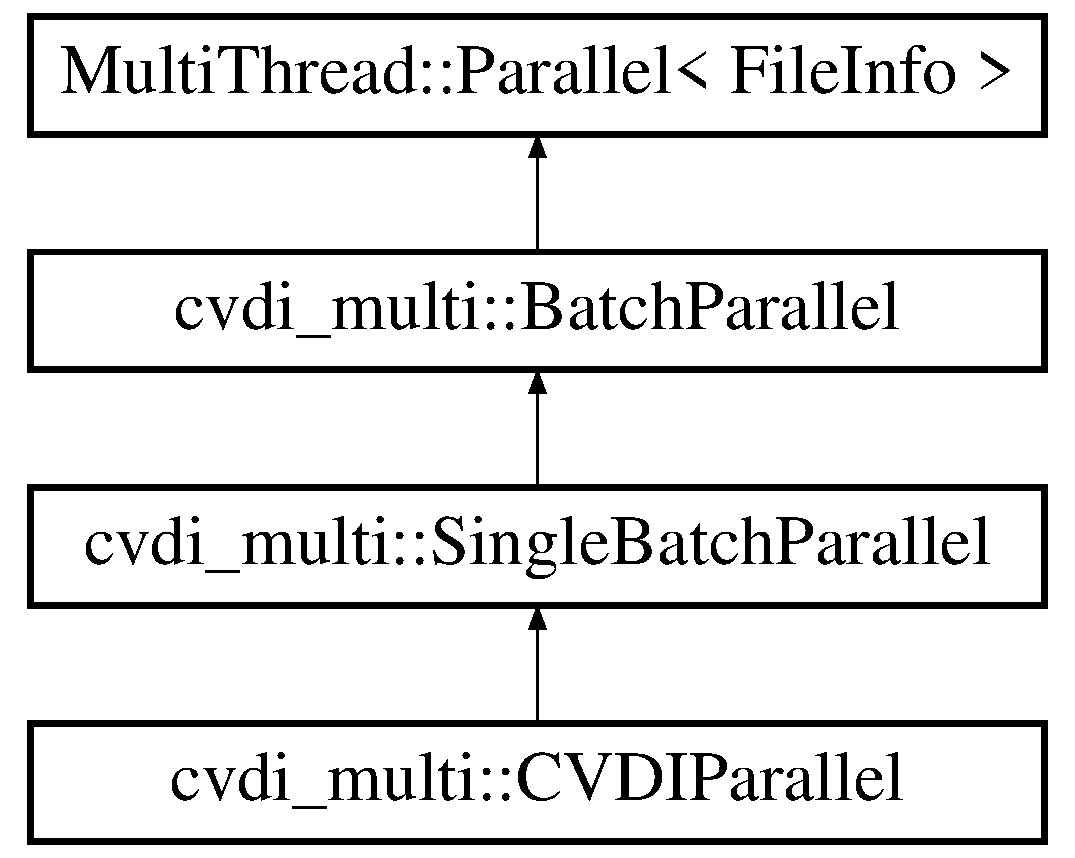
\includegraphics[height=4.000000cm]{classcvdi__multi_1_1SingleBatchParallel}
\end{center}
\end{figure}
\subsection*{Public Member Functions}
\begin{DoxyCompactItemize}
\item 
{\bfseries Single\+Batch\+Parallel} (const std\+::string \&file\+\_\+path)\hypertarget{classcvdi__multi_1_1SingleBatchParallel_ac209a23cedee901482dd96d878f85688}{}\label{classcvdi__multi_1_1SingleBatchParallel_ac209a23cedee901482dd96d878f85688}

\item 
virtual void \hyperlink{classcvdi__multi_1_1SingleBatchParallel_a6514a89e14f2724ab671ffd65d7c43c7}{Thread} (unsigned thread\+\_\+num, \hyperlink{classMultiThread_1_1SharedQueue}{Multi\+Thread\+::\+Shared\+Queue}$<$ File\+Info\+::\+Ptr $>$ $\ast$q)=0
\begin{DoxyCompactList}\small\item\em The main work thread. \end{DoxyCompactList}\item 
File\+Info\+::\+Ptr {\bfseries Next\+Item} (void)\hypertarget{classcvdi__multi_1_1SingleBatchParallel_a26f4c22424a0f3683e9a2f326adba590}{}\label{classcvdi__multi_1_1SingleBatchParallel_a26f4c22424a0f3683e9a2f326adba590}

\end{DoxyCompactItemize}


\subsection{Detailed Description}
Single file batch processing. 

\subsection{Member Function Documentation}
\index{cvdi\+\_\+multi\+::\+Single\+Batch\+Parallel@{cvdi\+\_\+multi\+::\+Single\+Batch\+Parallel}!Thread@{Thread}}
\index{Thread@{Thread}!cvdi\+\_\+multi\+::\+Single\+Batch\+Parallel@{cvdi\+\_\+multi\+::\+Single\+Batch\+Parallel}}
\subsubsection[{\texorpdfstring{Thread(unsigned thread\+\_\+num, Multi\+Thread\+::\+Shared\+Queue$<$ File\+Info\+::\+Ptr $>$ $\ast$q)=0}{Thread(unsigned thread_num, MultiThread::SharedQueue< FileInfo::Ptr > *q)=0}}]{\setlength{\rightskip}{0pt plus 5cm}virtual void cvdi\+\_\+multi\+::\+Single\+Batch\+Parallel\+::\+Thread (
\begin{DoxyParamCaption}
\item[{unsigned}]{thread\+\_\+num, }
\item[{{\bf Multi\+Thread\+::\+Shared\+Queue}$<$ File\+Info\+::\+Ptr $>$ $\ast$}]{q}
\end{DoxyParamCaption}
)\hspace{0.3cm}{\ttfamily [pure virtual]}}\hypertarget{classcvdi__multi_1_1SingleBatchParallel_a6514a89e14f2724ab671ffd65d7c43c7}{}\label{classcvdi__multi_1_1SingleBatchParallel_a6514a89e14f2724ab671ffd65d7c43c7}


The main work thread. 


\begin{DoxyParams}{Parameters}
{\em thread\+\_\+num} & a easy to read unique identifier for this thread. \\
\hline
{\em the} & work queue containing the trip files that this thread should process. \\
\hline
\end{DoxyParams}


Implements \hyperlink{classcvdi__multi_1_1BatchParallel_a23fd90da6768ad102e3ce5968ab11410}{cvdi\+\_\+multi\+::\+Batch\+Parallel}.



Implemented in \hyperlink{classcvdi__multi_1_1CVDIParallel_a7c256d91bb868873a1c6ce854c923c17}{cvdi\+\_\+multi\+::\+C\+V\+D\+I\+Parallel}.



The documentation for this class was generated from the following files\+:\begin{DoxyCompactItemize}
\item 
cvdi-\/src/cvdi-\/cl/include/cvdi\+\_\+multi.\+hpp\item 
cvdi-\/src/cvdi-\/cl/src/cvdi\+\_\+multi.\+cpp\end{DoxyCompactItemize}

\hypertarget{classcvdi__multi_1_1SingleFileInfo}{}\section{cvdi\+\_\+multi\+:\+:Single\+File\+Info Class Reference}
\label{classcvdi__multi_1_1SingleFileInfo}\index{cvdi\+\_\+multi\+::\+Single\+File\+Info@{cvdi\+\_\+multi\+::\+Single\+File\+Info}}


A class representing a file containing a single trip. Each instance can be annotated with auxiliary information. Size is used to distribute work across threads.  




{\ttfamily \#include $<$cvdi\+\_\+multi.\+hpp$>$}

Inheritance diagram for cvdi\+\_\+multi\+:\+:Single\+File\+Info\+:\begin{figure}[H]
\begin{center}
\leavevmode
\includegraphics[height=2.000000cm]{classcvdi__multi_1_1SingleFileInfo}
\end{center}
\end{figure}
\subsection*{Public Types}
\begin{DoxyCompactItemize}
\item 
using {\bfseries Ptr} = std\+::shared\+\_\+ptr$<$ \hyperlink{classcvdi__multi_1_1SingleFileInfo}{Single\+File\+Info} $>$\hypertarget{classcvdi__multi_1_1SingleFileInfo_a834ecd875a2083ef98c83f136e606711}{}\label{classcvdi__multi_1_1SingleFileInfo_a834ecd875a2083ef98c83f136e606711}

\end{DoxyCompactItemize}
\subsection*{Public Member Functions}
\begin{DoxyCompactItemize}
\item 
{\bfseries Single\+File\+Info} (const std\+::string \&file\+\_\+path)\hypertarget{classcvdi__multi_1_1SingleFileInfo_a3e05eee2e82576152680ac371a9b5a29}{}\label{classcvdi__multi_1_1SingleFileInfo_a3e05eee2e82576152680ac371a9b5a29}

\item 
{\bfseries Single\+File\+Info} (const std\+::string \&file\+\_\+path, const std\+::string \&aux\+\_\+data)\hypertarget{classcvdi__multi_1_1SingleFileInfo_a2e1b3e509271a53d1ea4ebe397b09c4b}{}\label{classcvdi__multi_1_1SingleFileInfo_a2e1b3e509271a53d1ea4ebe397b09c4b}

\item 
const std\+::string {\bfseries Get\+File\+Path} (void) const \hypertarget{classcvdi__multi_1_1SingleFileInfo_a7cd6386fb29f39cd32aab573619c7704}{}\label{classcvdi__multi_1_1SingleFileInfo_a7cd6386fb29f39cd32aab573619c7704}

\item 
const std\+::string {\bfseries Get\+Aux\+Data} (void) const \hypertarget{classcvdi__multi_1_1SingleFileInfo_a3792837adc62d140288c280ac2829356}{}\label{classcvdi__multi_1_1SingleFileInfo_a3792837adc62d140288c280ac2829356}

\end{DoxyCompactItemize}


\subsection{Detailed Description}
A class representing a file containing a single trip. Each instance can be annotated with auxiliary information. Size is used to distribute work across threads. 

The documentation for this class was generated from the following files\+:\begin{DoxyCompactItemize}
\item 
cvdi-\/src/cvdi-\/cl/include/cvdi\+\_\+multi.\+hpp\item 
cvdi-\/src/cvdi-\/cl/src/cvdi\+\_\+multi.\+cpp\end{DoxyCompactItemize}

\hypertarget{classspdlog_1_1sinks_1_1sink}{}\section{spdlog\+:\+:sinks\+:\+:sink Class Reference}
\label{classspdlog_1_1sinks_1_1sink}\index{spdlog\+::sinks\+::sink@{spdlog\+::sinks\+::sink}}
Inheritance diagram for spdlog\+:\+:sinks\+:\+:sink\+:\begin{figure}[H]
\begin{center}
\leavevmode
\includegraphics[height=12.000000cm]{classspdlog_1_1sinks_1_1sink}
\end{center}
\end{figure}
\subsection*{Public Member Functions}
\begin{DoxyCompactItemize}
\item 
virtual void {\bfseries log} (const \hyperlink{structspdlog_1_1details_1_1log__msg}{details\+::log\+\_\+msg} \&msg)=0\hypertarget{classspdlog_1_1sinks_1_1sink_a51d8f34ad79064e0dc13c6013236e427}{}\label{classspdlog_1_1sinks_1_1sink_a51d8f34ad79064e0dc13c6013236e427}

\item 
virtual void {\bfseries flush} ()=0\hypertarget{classspdlog_1_1sinks_1_1sink_a8a0674ae3bca8f1617aef820e23a2ccd}{}\label{classspdlog_1_1sinks_1_1sink_a8a0674ae3bca8f1617aef820e23a2ccd}

\item 
bool {\bfseries should\+\_\+log} (level\+::level\+\_\+enum msg\+\_\+level) const \hypertarget{classspdlog_1_1sinks_1_1sink_aee70cdd1f77473d658840447d3f3afff}{}\label{classspdlog_1_1sinks_1_1sink_aee70cdd1f77473d658840447d3f3afff}

\item 
void {\bfseries set\+\_\+level} (level\+::level\+\_\+enum log\+\_\+level)\hypertarget{classspdlog_1_1sinks_1_1sink_a038a91409395dca18a7ccca81622fd83}{}\label{classspdlog_1_1sinks_1_1sink_a038a91409395dca18a7ccca81622fd83}

\item 
level\+::level\+\_\+enum {\bfseries level} () const \hypertarget{classspdlog_1_1sinks_1_1sink_a026877b46301b9bd0d22afc65c2f3eca}{}\label{classspdlog_1_1sinks_1_1sink_a026877b46301b9bd0d22afc65c2f3eca}

\end{DoxyCompactItemize}


The documentation for this class was generated from the following file\+:\begin{DoxyCompactItemize}
\item 
cvdi-\/src/cvdi-\/cl/include/spdlog/sinks/sink.\+h\end{DoxyCompactItemize}

\hypertarget{classgeo_1_1Spatial}{}\section{geo\+:\+:Spatial Class Reference}
\label{classgeo_1_1Spatial}\index{geo\+::\+Spatial@{geo\+::\+Spatial}}


\hyperlink{classgeo_1_1Spatial}{Spatial} operator class.  




{\ttfamily \#include $<$geo.\+hpp$>$}

\subsection*{Public Member Functions}
\begin{DoxyCompactItemize}
\item 
double \hyperlink{classgeo_1_1Spatial_adcdd1f41c39d0999326828527c8e7aaa}{intercept} (const O\+G\+R\+Line\+String \&line\+\_\+string, const O\+G\+R\+Point \&point) const 
\begin{DoxyCompactList}\small\item\em Compute the geospatial intercept of point and a line string. The intercept value represents the point\textquotesingle{}s interpolation within the interval \mbox{[}0,1\mbox{]}. If the return value is not within this interval then the point does not intercept the line. A value of 0 means the point is on one end of the line and a value of 1 means the point is on the other end. \end{DoxyCompactList}\item 
double \hyperlink{classgeo_1_1Spatial_a5521d7ea795ff49abb99e324982764e4}{intercept} (const O\+G\+R\+Point \&point\+\_\+a, const O\+G\+R\+Point \&point\+\_\+b, const O\+G\+R\+Point \&point\+\_\+c) const 
\begin{DoxyCompactList}\small\item\em Compute the geospatial intercept of a line formed by points A and B with point C. The intercept value represents point C\textquotesingle{}s interpolation within the interval \mbox{[}0,1\mbox{]}. If the return value is not within this interval then the point does not intercept the line segment. A value of 0 means C is equal to A and a value of 1 means the C is equal to B. \end{DoxyCompactList}\item 
void \hyperlink{classgeo_1_1Spatial_abd029fbc910d1d983bb006f9729c4904}{intercept} (const O\+G\+R\+Point \&point\+\_\+a, const O\+G\+R\+Point \&point\+\_\+b, const O\+G\+R\+Point \&point\+\_\+c, O\+G\+R\+Point \&out) const 
\begin{DoxyCompactList}\small\item\em Compute the geospatial intercept point of a line formed by points A and B with point C. The intercept point represents the original point\textquotesingle{}s interpolated position on the line. The intercept point will be either A or B if the point C does not intercept the line segment (i.\+e. interpolated as an end point) \end{DoxyCompactList}\item 
void \hyperlink{classgeo_1_1Spatial_a01ef3e17941b265d3b21c9d3a618da18}{interpolate} (const O\+G\+R\+Point \&point\+\_\+a, const O\+G\+R\+Point \&point\+\_\+b, double fraction, O\+G\+R\+Point \&out) const 
\begin{DoxyCompactList}\small\item\em Get the point on a line given by points A and B and a fraction. If the fraction is less than 0 then point A is returned and if the fraction is greater than 1 then point B is returned. \end{DoxyCompactList}\item 
bool \hyperlink{classgeo_1_1Spatial_a4de3f6650935ef3ece0db3d19f06a5f9}{interpolate} (const O\+G\+R\+Line\+String \&line\+\_\+string, double \hyperlink{classgeo_1_1Spatial_a6bcfc529e8ab148e30cb58f243362eee}{length}, double fraction, O\+G\+R\+Point \&out) const 
\begin{DoxyCompactList}\small\item\em Get the point on a line string of given length and fraction. If the fraction is less than 0 then the first point of the line string is returned and if the fraction is greater than 1 then the last point of the line string is returned. \end{DoxyCompactList}\item 
bool \hyperlink{classgeo_1_1Spatial_a309e1932e955eee2a57d2104655e8080}{interpolate} (const O\+G\+R\+Line\+String \&line\+\_\+string, double fraction, O\+G\+R\+Point \&out) const 
\begin{DoxyCompactList}\small\item\em Get the point on a line string of given fraction. If the fraction is less than 0 then the first point of the line string is returned and if the fraction is greater than 1 then the last point of the line string is returned. \end{DoxyCompactList}\item 
double \hyperlink{classgeo_1_1Spatial_a9530b4b540b4601fa6254d2a30c17b95}{distance} (const O\+G\+R\+Point \&point\+\_\+a, const O\+G\+R\+Point \&point\+\_\+b) const 
\begin{DoxyCompactList}\small\item\em Get the distance in meters between two points. \end{DoxyCompactList}\item 
double \hyperlink{classgeo_1_1Spatial_a6bcfc529e8ab148e30cb58f243362eee}{length} (const O\+G\+R\+Line\+String \&line\+\_\+string) const 
\item 
void \hyperlink{classgeo_1_1Spatial_a6550ab40ef68eee2bc2345df92a65f37}{envelope\+\_\+for\+\_\+radius} (const O\+G\+R\+Point \&point, double radius, O\+G\+R\+Envelope \&envelope) const 
\item 
void \hyperlink{classgeo_1_1Spatial_a4d594e436dd265ed927e6ce4d3a8db42}{rect\+\_\+for\+\_\+radius} (const O\+G\+R\+Point \&point, double radius, C\+P\+L\+Rect\+Obj \&rect) const 
\item 
void \hyperlink{classgeo_1_1Spatial_aab7fbff6c1e0dbc56e58ff3065a435d2}{point\+\_\+from\+\_\+bearing} (double start\+\_\+lat, double start\+\_\+lon, double \hyperlink{classgeo_1_1Spatial_a9530b4b540b4601fa6254d2a30c17b95}{distance}, double bearing, double $\ast$lat\+\_\+out, double $\ast$lon\+\_\+out) const 
\item 
double \hyperlink{classgeo_1_1Spatial_abac49c2a0f02415321758d9cdbc86f92}{azimuth} (const O\+G\+R\+Point \&point\+\_\+a, const O\+G\+R\+Point \&point\+\_\+b, double fraction) const 
\item 
double \hyperlink{classgeo_1_1Spatial_a834e931e1879d3296e365b74215da09e}{azimuth} (const O\+G\+R\+Line\+String \&line\+\_\+string, double \hyperlink{classgeo_1_1Spatial_a6bcfc529e8ab148e30cb58f243362eee}{length}, double fraction) const 
\item 
double \hyperlink{classgeo_1_1Spatial_a2e45a6bce9ffd26b9d8546876747e118}{azimuth} (const O\+G\+R\+Line\+String \&line\+\_\+string, double fraction) const 
\item 
void \hyperlink{classgeo_1_1Spatial_a34a03dcb8afdca6fc2d4cfc3fd3025e6}{rect\+\_\+ring} (const O\+G\+R\+Point \&a, const O\+G\+R\+Point \&b, double width, double extension, O\+G\+R\+Linear\+Ring \&out) const 
\end{DoxyCompactItemize}
\subsection*{Static Public Member Functions}
\begin{DoxyCompactItemize}
\item 
static bool \hyperlink{classgeo_1_1Spatial_a038ae4ddfdb9c89ce9bb3d55f4e6daa7}{doubles\+\_\+are\+\_\+equal} (double a, double b, double epsilon)
\begin{DoxyCompactList}\small\item\em Uses epsilon values to compare double precision equality. \end{DoxyCompactList}\item 
static double \hyperlink{classgeo_1_1Spatial_a70141094fae0f0fabc90224bf1d7cd0f}{to\+\_\+radians} (double degrees)
\begin{DoxyCompactList}\small\item\em Convert decimal degrees to radians. \end{DoxyCompactList}\item 
static double \hyperlink{classgeo_1_1Spatial_a2bff1ce08e67dc3f6ca2ee90f97860e4}{to\+\_\+degrees} (double radians)
\begin{DoxyCompactList}\small\item\em Convert radians to decimal degrees. \end{DoxyCompactList}\item 
static double \hyperlink{classgeo_1_1Spatial_a820aa2d3891ef2c7c560cb71c88d24ba}{round} (double value)
\begin{DoxyCompactList}\small\item\em Round to a double precision number to k\+Precision. \end{DoxyCompactList}\item 
static double \hyperlink{classgeo_1_1Spatial_ae0055b6a137cb3159a097c70d3c7f375}{heading\+\_\+delta} (double a, double b)
\begin{DoxyCompactList}\small\item\em Compute the difference between two heading values in degrees. \end{DoxyCompactList}\end{DoxyCompactItemize}
\subsection*{Static Public Attributes}
\begin{DoxyCompactItemize}
\item 
static constexpr double \hyperlink{classgeo_1_1Spatial_a24d24121ccdc99cd841f3aeb744032ff}{k\+Pi} = 3.\+14159265358979323846\hypertarget{classgeo_1_1Spatial_a24d24121ccdc99cd841f3aeb744032ff}{}\label{classgeo_1_1Spatial_a24d24121ccdc99cd841f3aeb744032ff}

\begin{DoxyCompactList}\small\item\em Standard PI value used in degrees to radians conversions. \end{DoxyCompactList}\item 
static constexpr double \hyperlink{classgeo_1_1Spatial_a999c14d081785779ab54afc9d3ac61bb}{k\+G\+P\+S\+Epsilon} = std\+::numeric\+\_\+limits$<$double$>$\+::epsilon() $\ast$ 100.\+0\hypertarget{classgeo_1_1Spatial_a999c14d081785779ab54afc9d3ac61bb}{}\label{classgeo_1_1Spatial_a999c14d081785779ab54afc9d3ac61bb}

\begin{DoxyCompactList}\small\item\em G\+PS epsilon for comparing decimal G\+PS coordinates. \end{DoxyCompactList}\item 
static constexpr double \hyperlink{classgeo_1_1Spatial_a31720b63ae272b98283851a74a4d34d3}{k\+Intercept\+Epsilon} = std\+::sqrt(std\+::numeric\+\_\+limits$<$double$>$\+::epsilon()) $\ast$ 0.\+01\hypertarget{classgeo_1_1Spatial_a31720b63ae272b98283851a74a4d34d3}{}\label{classgeo_1_1Spatial_a31720b63ae272b98283851a74a4d34d3}

\begin{DoxyCompactList}\small\item\em The epsilon for comparing geospatial intercepts. \end{DoxyCompactList}\item 
static constexpr double \hyperlink{classgeo_1_1Spatial_adb250ee63cf19c7e9d2f691184521516}{k\+Earth\+RadiusM} = 6378137.\+0\hypertarget{classgeo_1_1Spatial_adb250ee63cf19c7e9d2f691184521516}{}\label{classgeo_1_1Spatial_adb250ee63cf19c7e9d2f691184521516}

\begin{DoxyCompactList}\small\item\em The Earth\textquotesingle{}s radius in meters. \end{DoxyCompactList}\item 
static constexpr double \hyperlink{classgeo_1_1Spatial_a317a6c113f7c71a94e706d47a19ed182}{k\+Precision} = 1\+E-\/8\hypertarget{classgeo_1_1Spatial_a317a6c113f7c71a94e706d47a19ed182}{}\label{classgeo_1_1Spatial_a317a6c113f7c71a94e706d47a19ed182}

\begin{DoxyCompactList}\small\item\em The precision used to round double values. \end{DoxyCompactList}\end{DoxyCompactItemize}


\subsection{Detailed Description}
\hyperlink{classgeo_1_1Spatial}{Spatial} operator class. 

\subsection{Member Function Documentation}
\index{geo\+::\+Spatial@{geo\+::\+Spatial}!azimuth@{azimuth}}
\index{azimuth@{azimuth}!geo\+::\+Spatial@{geo\+::\+Spatial}}
\subsubsection[{\texorpdfstring{azimuth(const O\+G\+R\+Point \&point\+\_\+a, const O\+G\+R\+Point \&point\+\_\+b, double fraction) const }{azimuth(const OGRPoint &point_a, const OGRPoint &point_b, double fraction) const }}]{\setlength{\rightskip}{0pt plus 5cm}double geo\+::\+Spatial\+::azimuth (
\begin{DoxyParamCaption}
\item[{const O\+G\+R\+Point \&}]{point\+\_\+a, }
\item[{const O\+G\+R\+Point \&}]{point\+\_\+b, }
\item[{double}]{fraction}
\end{DoxyParamCaption}
) const}\hypertarget{classgeo_1_1Spatial_abac49c2a0f02415321758d9cdbc86f92}{}\label{classgeo_1_1Spatial_abac49c2a0f02415321758d9cdbc86f92}
Compute the azimuth (bearing or heading) as degrees from north between two points A and B within the given fraction. If the fraction is less than 0 then the azimuth between A and B is returned and if the fraction is greater than 1 then the azimuth between B and A is returned.


\begin{DoxyParams}{Parameters}
{\em point\+\_\+a} & the first point \\
\hline
{\em point\+\_\+b} & the second point \\
\hline
{\em fraction} & the fraction in the line formed by point\+\_\+a and point\+\_\+b within the interval \mbox{[}0,1\mbox{]} \\
\hline
\end{DoxyParams}
\begin{DoxyReturn}{Returns}
the azimuth in degrees from north between point\+\_\+a and point\+\_\+b 
\end{DoxyReturn}
\index{geo\+::\+Spatial@{geo\+::\+Spatial}!azimuth@{azimuth}}
\index{azimuth@{azimuth}!geo\+::\+Spatial@{geo\+::\+Spatial}}
\subsubsection[{\texorpdfstring{azimuth(const O\+G\+R\+Line\+String \&line\+\_\+string, double length, double fraction) const }{azimuth(const OGRLineString &line_string, double length, double fraction) const }}]{\setlength{\rightskip}{0pt plus 5cm}double geo\+::\+Spatial\+::azimuth (
\begin{DoxyParamCaption}
\item[{const O\+G\+R\+Line\+String \&}]{line\+\_\+string, }
\item[{double}]{length, }
\item[{double}]{fraction}
\end{DoxyParamCaption}
) const}\hypertarget{classgeo_1_1Spatial_a834e931e1879d3296e365b74215da09e}{}\label{classgeo_1_1Spatial_a834e931e1879d3296e365b74215da09e}
Compute the azimuth (bearing or heading) as degrees from north for a line string with the given length and fraction. If the fraction is less than 0 then the azimuth between the first two points of the line string is returned. If the fraction is greater than 1 then the azimuth between the last two points is returned.


\begin{DoxyParams}{Parameters}
{\em line\+\_\+string} & the line string \\
\hline
{\em fraction} & the fraction on the line string within the interval \mbox{[}0,1\mbox{]} \\
\hline
{\em length} & the length of the line string to use \\
\hline
\end{DoxyParams}
\begin{DoxyReturn}{Returns}
the azimuth in degrees from north of the line string 
\end{DoxyReturn}
\index{geo\+::\+Spatial@{geo\+::\+Spatial}!azimuth@{azimuth}}
\index{azimuth@{azimuth}!geo\+::\+Spatial@{geo\+::\+Spatial}}
\subsubsection[{\texorpdfstring{azimuth(const O\+G\+R\+Line\+String \&line\+\_\+string, double fraction) const }{azimuth(const OGRLineString &line_string, double fraction) const }}]{\setlength{\rightskip}{0pt plus 5cm}double geo\+::\+Spatial\+::azimuth (
\begin{DoxyParamCaption}
\item[{const O\+G\+R\+Line\+String \&}]{line\+\_\+string, }
\item[{double}]{fraction}
\end{DoxyParamCaption}
) const}\hypertarget{classgeo_1_1Spatial_a2e45a6bce9ffd26b9d8546876747e118}{}\label{classgeo_1_1Spatial_a2e45a6bce9ffd26b9d8546876747e118}
Compute the azimuth (bearing or heading) as degrees from north for a line string with the given fraction. If the fraction is less than 0 then the azimuth between the first two points of the line string is returned. If the fraction is greater than 1 then the azimuth between the last two points is returned.


\begin{DoxyParams}{Parameters}
{\em line\+\_\+string} & the line string \\
\hline
{\em fraction} & the fraction on the line string within the interval \mbox{[}0,1\mbox{]} \\
\hline
\end{DoxyParams}
\begin{DoxyReturn}{Returns}
the azimuth in degrees from north of the line string 
\end{DoxyReturn}
\index{geo\+::\+Spatial@{geo\+::\+Spatial}!distance@{distance}}
\index{distance@{distance}!geo\+::\+Spatial@{geo\+::\+Spatial}}
\subsubsection[{\texorpdfstring{distance(const O\+G\+R\+Point \&point\+\_\+a, const O\+G\+R\+Point \&point\+\_\+b) const }{distance(const OGRPoint &point_a, const OGRPoint &point_b) const }}]{\setlength{\rightskip}{0pt plus 5cm}double geo\+::\+Spatial\+::distance (
\begin{DoxyParamCaption}
\item[{const O\+G\+R\+Point \&}]{point\+\_\+a, }
\item[{const O\+G\+R\+Point \&}]{point\+\_\+b}
\end{DoxyParamCaption}
) const}\hypertarget{classgeo_1_1Spatial_a9530b4b540b4601fa6254d2a30c17b95}{}\label{classgeo_1_1Spatial_a9530b4b540b4601fa6254d2a30c17b95}


Get the distance in meters between two points. 


\begin{DoxyParams}{Parameters}
{\em point\+\_\+a} & the first point \\
\hline
{\em point\+\_\+a} & the second point \\
\hline
\end{DoxyParams}
\begin{DoxyReturn}{Returns}
the distance between point\+\_\+a and point\+\_\+b 
\end{DoxyReturn}
\index{geo\+::\+Spatial@{geo\+::\+Spatial}!doubles\+\_\+are\+\_\+equal@{doubles\+\_\+are\+\_\+equal}}
\index{doubles\+\_\+are\+\_\+equal@{doubles\+\_\+are\+\_\+equal}!geo\+::\+Spatial@{geo\+::\+Spatial}}
\subsubsection[{\texorpdfstring{doubles\+\_\+are\+\_\+equal(double a, double b, double epsilon)}{doubles_are_equal(double a, double b, double epsilon)}}]{\setlength{\rightskip}{0pt plus 5cm}static bool geo\+::\+Spatial\+::doubles\+\_\+are\+\_\+equal (
\begin{DoxyParamCaption}
\item[{double}]{a, }
\item[{double}]{b, }
\item[{double}]{epsilon}
\end{DoxyParamCaption}
)\hspace{0.3cm}{\ttfamily [inline]}, {\ttfamily [static]}}\hypertarget{classgeo_1_1Spatial_a038ae4ddfdb9c89ce9bb3d55f4e6daa7}{}\label{classgeo_1_1Spatial_a038ae4ddfdb9c89ce9bb3d55f4e6daa7}


Uses epsilon values to compare double precision equality. 


\begin{DoxyParams}{Parameters}
{\em a} & the first double \\
\hline
{\em b} & the second double \\
\hline
{\em epsilon} & the epsilon used for the equality comparison \\
\hline
\end{DoxyParams}
\begin{DoxyReturn}{Returns}
true if the absolute value difference between the doubles is less than the epsilon, false otherwise 
\end{DoxyReturn}
\index{geo\+::\+Spatial@{geo\+::\+Spatial}!envelope\+\_\+for\+\_\+radius@{envelope\+\_\+for\+\_\+radius}}
\index{envelope\+\_\+for\+\_\+radius@{envelope\+\_\+for\+\_\+radius}!geo\+::\+Spatial@{geo\+::\+Spatial}}
\subsubsection[{\texorpdfstring{envelope\+\_\+for\+\_\+radius(const O\+G\+R\+Point \&point, double radius, O\+G\+R\+Envelope \&envelope) const }{envelope_for_radius(const OGRPoint &point, double radius, OGREnvelope &envelope) const }}]{\setlength{\rightskip}{0pt plus 5cm}void geo\+::\+Spatial\+::envelope\+\_\+for\+\_\+radius (
\begin{DoxyParamCaption}
\item[{const O\+G\+R\+Point \&}]{point, }
\item[{double}]{radius, }
\item[{O\+G\+R\+Envelope \&}]{envelope}
\end{DoxyParamCaption}
) const}\hypertarget{classgeo_1_1Spatial_a6550ab40ef68eee2bc2345df92a65f37}{}\label{classgeo_1_1Spatial_a6550ab40ef68eee2bc2345df92a65f37}
Make an O\+G\+R\+Envelope bounding box for a point and given radius.


\begin{DoxyParams}{Parameters}
{\em point} & the center of the bounding box \\
\hline
{\em radius} & the half-\/width of the box in meters \\
\hline
{\em envelope} & the resulting bounding box as an O\+G\+R\+Envelope \\
\hline
\end{DoxyParams}
\index{geo\+::\+Spatial@{geo\+::\+Spatial}!heading\+\_\+delta@{heading\+\_\+delta}}
\index{heading\+\_\+delta@{heading\+\_\+delta}!geo\+::\+Spatial@{geo\+::\+Spatial}}
\subsubsection[{\texorpdfstring{heading\+\_\+delta(double a, double b)}{heading_delta(double a, double b)}}]{\setlength{\rightskip}{0pt plus 5cm}static double geo\+::\+Spatial\+::heading\+\_\+delta (
\begin{DoxyParamCaption}
\item[{double}]{a, }
\item[{double}]{b}
\end{DoxyParamCaption}
)\hspace{0.3cm}{\ttfamily [inline]}, {\ttfamily [static]}}\hypertarget{classgeo_1_1Spatial_ae0055b6a137cb3159a097c70d3c7f375}{}\label{classgeo_1_1Spatial_ae0055b6a137cb3159a097c70d3c7f375}


Compute the difference between two heading values in degrees. 


\begin{DoxyParams}{Parameters}
{\em a} & the first heading \\
\hline
{\em b} & the second heading \\
\hline
\end{DoxyParams}
\begin{DoxyReturn}{Returns}
the difference between the two headings in degrees 
\end{DoxyReturn}
\index{geo\+::\+Spatial@{geo\+::\+Spatial}!intercept@{intercept}}
\index{intercept@{intercept}!geo\+::\+Spatial@{geo\+::\+Spatial}}
\subsubsection[{\texorpdfstring{intercept(const O\+G\+R\+Line\+String \&line\+\_\+string, const O\+G\+R\+Point \&point) const }{intercept(const OGRLineString &line_string, const OGRPoint &point) const }}]{\setlength{\rightskip}{0pt plus 5cm}double geo\+::\+Spatial\+::intercept (
\begin{DoxyParamCaption}
\item[{const O\+G\+R\+Line\+String \&}]{line\+\_\+string, }
\item[{const O\+G\+R\+Point \&}]{point}
\end{DoxyParamCaption}
) const}\hypertarget{classgeo_1_1Spatial_adcdd1f41c39d0999326828527c8e7aaa}{}\label{classgeo_1_1Spatial_adcdd1f41c39d0999326828527c8e7aaa}


Compute the geospatial intercept of point and a line string. The intercept value represents the point\textquotesingle{}s interpolation within the interval \mbox{[}0,1\mbox{]}. If the return value is not within this interval then the point does not intercept the line. A value of 0 means the point is on one end of the line and a value of 1 means the point is on the other end. 


\begin{DoxyParams}{Parameters}
{\em line\+\_\+string} & the line string \\
\hline
{\em point} & the point \\
\hline
\end{DoxyParams}
\begin{DoxyReturn}{Returns}
the intercept value 
\end{DoxyReturn}
\index{geo\+::\+Spatial@{geo\+::\+Spatial}!intercept@{intercept}}
\index{intercept@{intercept}!geo\+::\+Spatial@{geo\+::\+Spatial}}
\subsubsection[{\texorpdfstring{intercept(const O\+G\+R\+Point \&point\+\_\+a, const O\+G\+R\+Point \&point\+\_\+b, const O\+G\+R\+Point \&point\+\_\+c) const }{intercept(const OGRPoint &point_a, const OGRPoint &point_b, const OGRPoint &point_c) const }}]{\setlength{\rightskip}{0pt plus 5cm}double geo\+::\+Spatial\+::intercept (
\begin{DoxyParamCaption}
\item[{const O\+G\+R\+Point \&}]{point\+\_\+a, }
\item[{const O\+G\+R\+Point \&}]{point\+\_\+b, }
\item[{const O\+G\+R\+Point \&}]{point\+\_\+c}
\end{DoxyParamCaption}
) const}\hypertarget{classgeo_1_1Spatial_a5521d7ea795ff49abb99e324982764e4}{}\label{classgeo_1_1Spatial_a5521d7ea795ff49abb99e324982764e4}


Compute the geospatial intercept of a line formed by points A and B with point C. The intercept value represents point C\textquotesingle{}s interpolation within the interval \mbox{[}0,1\mbox{]}. If the return value is not within this interval then the point does not intercept the line segment. A value of 0 means C is equal to A and a value of 1 means the C is equal to B. 


\begin{DoxyParams}{Parameters}
{\em point\+\_\+a} & the first point of the line \\
\hline
{\em point\+\_\+b} & the second point of the line \\
\hline
{\em point\+\_\+c} & the third point, not on the line \\
\hline
\end{DoxyParams}
\begin{DoxyReturn}{Returns}
the intercept value 
\end{DoxyReturn}
\index{geo\+::\+Spatial@{geo\+::\+Spatial}!intercept@{intercept}}
\index{intercept@{intercept}!geo\+::\+Spatial@{geo\+::\+Spatial}}
\subsubsection[{\texorpdfstring{intercept(const O\+G\+R\+Point \&point\+\_\+a, const O\+G\+R\+Point \&point\+\_\+b, const O\+G\+R\+Point \&point\+\_\+c, O\+G\+R\+Point \&out) const }{intercept(const OGRPoint &point_a, const OGRPoint &point_b, const OGRPoint &point_c, OGRPoint &out) const }}]{\setlength{\rightskip}{0pt plus 5cm}void geo\+::\+Spatial\+::intercept (
\begin{DoxyParamCaption}
\item[{const O\+G\+R\+Point \&}]{point\+\_\+a, }
\item[{const O\+G\+R\+Point \&}]{point\+\_\+b, }
\item[{const O\+G\+R\+Point \&}]{point\+\_\+c, }
\item[{O\+G\+R\+Point \&}]{out}
\end{DoxyParamCaption}
) const}\hypertarget{classgeo_1_1Spatial_abd029fbc910d1d983bb006f9729c4904}{}\label{classgeo_1_1Spatial_abd029fbc910d1d983bb006f9729c4904}


Compute the geospatial intercept point of a line formed by points A and B with point C. The intercept point represents the original point\textquotesingle{}s interpolated position on the line. The intercept point will be either A or B if the point C does not intercept the line segment (i.\+e. interpolated as an end point) 


\begin{DoxyParams}{Parameters}
{\em point\+\_\+a} & the first point of the line \\
\hline
{\em point\+\_\+b} & the second point of the line \\
\hline
{\em point\+\_\+c} & the third point, not on the line \\
\hline
{\em out} & the intercept point of point\+\_\+c the line \\
\hline
\end{DoxyParams}
\index{geo\+::\+Spatial@{geo\+::\+Spatial}!interpolate@{interpolate}}
\index{interpolate@{interpolate}!geo\+::\+Spatial@{geo\+::\+Spatial}}
\subsubsection[{\texorpdfstring{interpolate(const O\+G\+R\+Point \&point\+\_\+a, const O\+G\+R\+Point \&point\+\_\+b, double fraction, O\+G\+R\+Point \&out) const }{interpolate(const OGRPoint &point_a, const OGRPoint &point_b, double fraction, OGRPoint &out) const }}]{\setlength{\rightskip}{0pt plus 5cm}void geo\+::\+Spatial\+::interpolate (
\begin{DoxyParamCaption}
\item[{const O\+G\+R\+Point \&}]{point\+\_\+a, }
\item[{const O\+G\+R\+Point \&}]{point\+\_\+b, }
\item[{double}]{fraction, }
\item[{O\+G\+R\+Point \&}]{out}
\end{DoxyParamCaption}
) const}\hypertarget{classgeo_1_1Spatial_a01ef3e17941b265d3b21c9d3a618da18}{}\label{classgeo_1_1Spatial_a01ef3e17941b265d3b21c9d3a618da18}


Get the point on a line given by points A and B and a fraction. If the fraction is less than 0 then point A is returned and if the fraction is greater than 1 then point B is returned. 


\begin{DoxyParams}{Parameters}
{\em point\+\_\+a} & the first point of the line \\
\hline
{\em point\+\_\+b} & the second point of the line \\
\hline
{\em fraction} & the fraction representing the position of the point on the line \\
\hline
{\em out} & the interpolated point between point\+\_\+a and point\+\_\+b \\
\hline
\end{DoxyParams}
\index{geo\+::\+Spatial@{geo\+::\+Spatial}!interpolate@{interpolate}}
\index{interpolate@{interpolate}!geo\+::\+Spatial@{geo\+::\+Spatial}}
\subsubsection[{\texorpdfstring{interpolate(const O\+G\+R\+Line\+String \&line\+\_\+string, double length, double fraction, O\+G\+R\+Point \&out) const }{interpolate(const OGRLineString &line_string, double length, double fraction, OGRPoint &out) const }}]{\setlength{\rightskip}{0pt plus 5cm}bool geo\+::\+Spatial\+::interpolate (
\begin{DoxyParamCaption}
\item[{const O\+G\+R\+Line\+String \&}]{line\+\_\+string, }
\item[{double}]{length, }
\item[{double}]{fraction, }
\item[{O\+G\+R\+Point \&}]{out}
\end{DoxyParamCaption}
) const}\hypertarget{classgeo_1_1Spatial_a4de3f6650935ef3ece0db3d19f06a5f9}{}\label{classgeo_1_1Spatial_a4de3f6650935ef3ece0db3d19f06a5f9}


Get the point on a line string of given length and fraction. If the fraction is less than 0 then the first point of the line string is returned and if the fraction is greater than 1 then the last point of the line string is returned. 


\begin{DoxyParams}{Parameters}
{\em line\+\_\+string} & the line string \\
\hline
{\em length} & the length of the line string to use \\
\hline
{\em fraction} & the fraction representing the position of the point on the line, within the given length \\
\hline
{\em out} & the interpolated point on line\+\_\+string \\
\hline
\end{DoxyParams}
\index{geo\+::\+Spatial@{geo\+::\+Spatial}!interpolate@{interpolate}}
\index{interpolate@{interpolate}!geo\+::\+Spatial@{geo\+::\+Spatial}}
\subsubsection[{\texorpdfstring{interpolate(const O\+G\+R\+Line\+String \&line\+\_\+string, double fraction, O\+G\+R\+Point \&out) const }{interpolate(const OGRLineString &line_string, double fraction, OGRPoint &out) const }}]{\setlength{\rightskip}{0pt plus 5cm}bool geo\+::\+Spatial\+::interpolate (
\begin{DoxyParamCaption}
\item[{const O\+G\+R\+Line\+String \&}]{line\+\_\+string, }
\item[{double}]{fraction, }
\item[{O\+G\+R\+Point \&}]{out}
\end{DoxyParamCaption}
) const}\hypertarget{classgeo_1_1Spatial_a309e1932e955eee2a57d2104655e8080}{}\label{classgeo_1_1Spatial_a309e1932e955eee2a57d2104655e8080}


Get the point on a line string of given fraction. If the fraction is less than 0 then the first point of the line string is returned and if the fraction is greater than 1 then the last point of the line string is returned. 


\begin{DoxyParams}{Parameters}
{\em line\+\_\+string} & the line string \\
\hline
{\em fraction} & the fraction representing the position of the point on the line, within the given length \\
\hline
{\em out} & the interpolated point \\
\hline
\end{DoxyParams}
\index{geo\+::\+Spatial@{geo\+::\+Spatial}!length@{length}}
\index{length@{length}!geo\+::\+Spatial@{geo\+::\+Spatial}}
\subsubsection[{\texorpdfstring{length(const O\+G\+R\+Line\+String \&line\+\_\+string) const }{length(const OGRLineString &line_string) const }}]{\setlength{\rightskip}{0pt plus 5cm}double geo\+::\+Spatial\+::length (
\begin{DoxyParamCaption}
\item[{const O\+G\+R\+Line\+String \&}]{line\+\_\+string}
\end{DoxyParamCaption}
) const}\hypertarget{classgeo_1_1Spatial_a6bcfc529e8ab148e30cb58f243362eee}{}\label{classgeo_1_1Spatial_a6bcfc529e8ab148e30cb58f243362eee}
Get the length in meters of a line string.


\begin{DoxyParams}{Parameters}
{\em line\+\_\+string} & the line string \\
\hline
\end{DoxyParams}
\begin{DoxyReturn}{Returns}
the length of line\+\_\+string 
\end{DoxyReturn}
\index{geo\+::\+Spatial@{geo\+::\+Spatial}!point\+\_\+from\+\_\+bearing@{point\+\_\+from\+\_\+bearing}}
\index{point\+\_\+from\+\_\+bearing@{point\+\_\+from\+\_\+bearing}!geo\+::\+Spatial@{geo\+::\+Spatial}}
\subsubsection[{\texorpdfstring{point\+\_\+from\+\_\+bearing(double start\+\_\+lat, double start\+\_\+lon, double distance, double bearing, double $\ast$lat\+\_\+out, double $\ast$lon\+\_\+out) const }{point_from_bearing(double start_lat, double start_lon, double distance, double bearing, double *lat_out, double *lon_out) const }}]{\setlength{\rightskip}{0pt plus 5cm}void geo\+::\+Spatial\+::point\+\_\+from\+\_\+bearing (
\begin{DoxyParamCaption}
\item[{double}]{start\+\_\+lat, }
\item[{double}]{start\+\_\+lon, }
\item[{double}]{distance, }
\item[{double}]{bearing, }
\item[{double $\ast$}]{lat\+\_\+out, }
\item[{double $\ast$}]{lon\+\_\+out}
\end{DoxyParamCaption}
) const}\hypertarget{classgeo_1_1Spatial_aab7fbff6c1e0dbc56e58ff3065a435d2}{}\label{classgeo_1_1Spatial_aab7fbff6c1e0dbc56e58ff3065a435d2}
Find a new point from start position, given a bearing and distance.


\begin{DoxyParams}{Parameters}
{\em start\+\_\+lat} & the latitude of the starting position \\
\hline
{\em start\+\_\+lon} & the longitude of the starting position \\
\hline
{\em distance} & the distance between the new point and starting position \\
\hline
{\em bearing} & the bearing from the starting position and new point \\
\hline
{\em lat\+\_\+out} & pointer to the new points latitude \\
\hline
{\em lon\+\_\+out} & pointer to the new point longitude \\
\hline
\end{DoxyParams}
\index{geo\+::\+Spatial@{geo\+::\+Spatial}!rect\+\_\+for\+\_\+radius@{rect\+\_\+for\+\_\+radius}}
\index{rect\+\_\+for\+\_\+radius@{rect\+\_\+for\+\_\+radius}!geo\+::\+Spatial@{geo\+::\+Spatial}}
\subsubsection[{\texorpdfstring{rect\+\_\+for\+\_\+radius(const O\+G\+R\+Point \&point, double radius, C\+P\+L\+Rect\+Obj \&rect) const }{rect_for_radius(const OGRPoint &point, double radius, CPLRectObj &rect) const }}]{\setlength{\rightskip}{0pt plus 5cm}void geo\+::\+Spatial\+::rect\+\_\+for\+\_\+radius (
\begin{DoxyParamCaption}
\item[{const O\+G\+R\+Point \&}]{point, }
\item[{double}]{radius, }
\item[{C\+P\+L\+Rect\+Obj \&}]{rect}
\end{DoxyParamCaption}
) const}\hypertarget{classgeo_1_1Spatial_a4d594e436dd265ed927e6ce4d3a8db42}{}\label{classgeo_1_1Spatial_a4d594e436dd265ed927e6ce4d3a8db42}
Make a C\+P\+L\+Rect\+Obj bounding box for a point and given radius.


\begin{DoxyParams}{Parameters}
{\em point} & the center of the bounding box \\
\hline
{\em radius} & the half-\/width of the box in meters \\
\hline
{\em envelope} & the resulting bounding box as a C\+P\+L\+Rect\+Obj \\
\hline
\end{DoxyParams}
\index{geo\+::\+Spatial@{geo\+::\+Spatial}!rect\+\_\+ring@{rect\+\_\+ring}}
\index{rect\+\_\+ring@{rect\+\_\+ring}!geo\+::\+Spatial@{geo\+::\+Spatial}}
\subsubsection[{\texorpdfstring{rect\+\_\+ring(const O\+G\+R\+Point \&a, const O\+G\+R\+Point \&b, double width, double extension, O\+G\+R\+Linear\+Ring \&out) const }{rect_ring(const OGRPoint &a, const OGRPoint &b, double width, double extension, OGRLinearRing &out) const }}]{\setlength{\rightskip}{0pt plus 5cm}void geo\+::\+Spatial\+::rect\+\_\+ring (
\begin{DoxyParamCaption}
\item[{const O\+G\+R\+Point \&}]{a, }
\item[{const O\+G\+R\+Point \&}]{b, }
\item[{double}]{width, }
\item[{double}]{extension, }
\item[{O\+G\+R\+Linear\+Ring \&}]{out}
\end{DoxyParamCaption}
) const}\hypertarget{classgeo_1_1Spatial_a34a03dcb8afdca6fc2d4cfc3fd3025e6}{}\label{classgeo_1_1Spatial_a34a03dcb8afdca6fc2d4cfc3fd3025e6}
Create a rectangle about two points A and B as an O\+G\+R\+Linear\+Ring. The rectangle will have a width equal to the given width and length equal to the distance between A and B plus the given extension.


\begin{DoxyParams}{Parameters}
{\em a} & the first point \\
\hline
{\em b} & the second point \\
\hline
{\em width} & the width of rectangle in meters \\
\hline
{\em extension} & the length extension of the rectangle in meters \\
\hline
{\em out} & the O\+G\+R\+Linear\+Ring representing the newly created rectangle \\
\hline
\end{DoxyParams}
\index{geo\+::\+Spatial@{geo\+::\+Spatial}!round@{round}}
\index{round@{round}!geo\+::\+Spatial@{geo\+::\+Spatial}}
\subsubsection[{\texorpdfstring{round(double value)}{round(double value)}}]{\setlength{\rightskip}{0pt plus 5cm}static double geo\+::\+Spatial\+::round (
\begin{DoxyParamCaption}
\item[{double}]{value}
\end{DoxyParamCaption}
)\hspace{0.3cm}{\ttfamily [inline]}, {\ttfamily [static]}}\hypertarget{classgeo_1_1Spatial_a820aa2d3891ef2c7c560cb71c88d24ba}{}\label{classgeo_1_1Spatial_a820aa2d3891ef2c7c560cb71c88d24ba}


Round to a double precision number to k\+Precision. 


\begin{DoxyParams}{Parameters}
{\em value} & the double value to round \\
\hline
\end{DoxyParams}
\begin{DoxyReturn}{Returns}
the rounded value 
\end{DoxyReturn}
\index{geo\+::\+Spatial@{geo\+::\+Spatial}!to\+\_\+degrees@{to\+\_\+degrees}}
\index{to\+\_\+degrees@{to\+\_\+degrees}!geo\+::\+Spatial@{geo\+::\+Spatial}}
\subsubsection[{\texorpdfstring{to\+\_\+degrees(double radians)}{to_degrees(double radians)}}]{\setlength{\rightskip}{0pt plus 5cm}static double geo\+::\+Spatial\+::to\+\_\+degrees (
\begin{DoxyParamCaption}
\item[{double}]{radians}
\end{DoxyParamCaption}
)\hspace{0.3cm}{\ttfamily [inline]}, {\ttfamily [static]}}\hypertarget{classgeo_1_1Spatial_a2bff1ce08e67dc3f6ca2ee90f97860e4}{}\label{classgeo_1_1Spatial_a2bff1ce08e67dc3f6ca2ee90f97860e4}


Convert radians to decimal degrees. 


\begin{DoxyParams}{Parameters}
{\em radians} & the radians value to convert \\
\hline
\end{DoxyParams}
\begin{DoxyReturn}{Returns}
the converted value in degrees 
\end{DoxyReturn}
\index{geo\+::\+Spatial@{geo\+::\+Spatial}!to\+\_\+radians@{to\+\_\+radians}}
\index{to\+\_\+radians@{to\+\_\+radians}!geo\+::\+Spatial@{geo\+::\+Spatial}}
\subsubsection[{\texorpdfstring{to\+\_\+radians(double degrees)}{to_radians(double degrees)}}]{\setlength{\rightskip}{0pt plus 5cm}static double geo\+::\+Spatial\+::to\+\_\+radians (
\begin{DoxyParamCaption}
\item[{double}]{degrees}
\end{DoxyParamCaption}
)\hspace{0.3cm}{\ttfamily [inline]}, {\ttfamily [static]}}\hypertarget{classgeo_1_1Spatial_a70141094fae0f0fabc90224bf1d7cd0f}{}\label{classgeo_1_1Spatial_a70141094fae0f0fabc90224bf1d7cd0f}


Convert decimal degrees to radians. 


\begin{DoxyParams}{Parameters}
{\em degrees} & the decimal degree value to convert \\
\hline
\end{DoxyParams}
\begin{DoxyReturn}{Returns}
the converted value in radians 
\end{DoxyReturn}


The documentation for this class was generated from the following files\+:\begin{DoxyCompactItemize}
\item 
cvdi-\/src/geo/include/geo.\+hpp\item 
cvdi-\/src/geo/src/geo.\+cpp\end{DoxyCompactItemize}

\hypertarget{classspdlog_1_1spdlog__ex}{}\section{spdlog\+:\+:spdlog\+\_\+ex Class Reference}
\label{classspdlog_1_1spdlog__ex}\index{spdlog\+::spdlog\+\_\+ex@{spdlog\+::spdlog\+\_\+ex}}
Inheritance diagram for spdlog\+:\+:spdlog\+\_\+ex\+:\begin{figure}[H]
\begin{center}
\leavevmode
\includegraphics[height=2.000000cm]{classspdlog_1_1spdlog__ex}
\end{center}
\end{figure}
\subsection*{Public Member Functions}
\begin{DoxyCompactItemize}
\item 
{\bfseries spdlog\+\_\+ex} (const std\+::string \&msg)\hypertarget{classspdlog_1_1spdlog__ex_a278ea1931ba954109480a619ef5ac945}{}\label{classspdlog_1_1spdlog__ex_a278ea1931ba954109480a619ef5ac945}

\item 
{\bfseries spdlog\+\_\+ex} (const std\+::string \&msg, int last\+\_\+errno)\hypertarget{classspdlog_1_1spdlog__ex_a0758933dd1e6c4c8e76bb8e7134f7d9b}{}\label{classspdlog_1_1spdlog__ex_a0758933dd1e6c4c8e76bb8e7134f7d9b}

\item 
const char $\ast$ {\bfseries what} () const S\+P\+D\+L\+O\+G\+\_\+\+N\+O\+E\+X\+C\+E\+PT override\hypertarget{classspdlog_1_1spdlog__ex_a9a9b9a7981e472cad06d453e368b6195}{}\label{classspdlog_1_1spdlog__ex_a9a9b9a7981e472cad06d453e368b6195}

\end{DoxyCompactItemize}


The documentation for this class was generated from the following file\+:\begin{DoxyCompactItemize}
\item 
cvdi-\/src/cvdi-\/cl/include/spdlog/common.\+h\end{DoxyCompactItemize}

\hypertarget{classspdlog_1_1SPDLOG__FINAL}{}\section{spdlog\+:\+:S\+P\+D\+L\+O\+G\+\_\+\+F\+I\+N\+AL Class Reference}
\label{classspdlog_1_1SPDLOG__FINAL}\index{spdlog\+::\+S\+P\+D\+L\+O\+G\+\_\+\+F\+I\+N\+AL@{spdlog\+::\+S\+P\+D\+L\+O\+G\+\_\+\+F\+I\+N\+AL}}
Inheritance diagram for spdlog\+:\+:S\+P\+D\+L\+O\+G\+\_\+\+F\+I\+N\+AL\+:\begin{figure}[H]
\begin{center}
\leavevmode
\includegraphics[height=2.000000cm]{classspdlog_1_1SPDLOG__FINAL}
\end{center}
\end{figure}
\subsection*{Public Member Functions}
\begin{DoxyCompactItemize}
\item 
{\footnotesize template$<$class It $>$ }\\{\bfseries async\+\_\+logger} (const std\+::string \&name, const It \&begin, const It \&end, size\+\_\+t queue\+\_\+size, const async\+\_\+overflow\+\_\+policy overflow\+\_\+policy=async\+\_\+overflow\+\_\+policy\+::block\+\_\+retry, const std\+::function$<$ void()$>$ \&worker\+\_\+warmup\+\_\+cb=nullptr, const std\+::chrono\+::milliseconds \&flush\+\_\+interval\+\_\+ms=std\+::chrono\+::milliseconds\+::zero(), const std\+::function$<$ void()$>$ \&worker\+\_\+teardown\+\_\+cb=nullptr)\hypertarget{classspdlog_1_1SPDLOG__FINAL_a8d7804abd9cfdf2258beecc99e91d15d}{}\label{classspdlog_1_1SPDLOG__FINAL_a8d7804abd9cfdf2258beecc99e91d15d}

\item 
{\bfseries async\+\_\+logger} (const std\+::string \&logger\+\_\+name, sinks\+\_\+init\+\_\+list sinks, size\+\_\+t queue\+\_\+size, const async\+\_\+overflow\+\_\+policy overflow\+\_\+policy=async\+\_\+overflow\+\_\+policy\+::block\+\_\+retry, const std\+::function$<$ void()$>$ \&worker\+\_\+warmup\+\_\+cb=nullptr, const std\+::chrono\+::milliseconds \&flush\+\_\+interval\+\_\+ms=std\+::chrono\+::milliseconds\+::zero(), const std\+::function$<$ void()$>$ \&worker\+\_\+teardown\+\_\+cb=nullptr)\hypertarget{classspdlog_1_1SPDLOG__FINAL_a855d21b6ac96d191a4ed339a97d73e5d}{}\label{classspdlog_1_1SPDLOG__FINAL_a855d21b6ac96d191a4ed339a97d73e5d}

\item 
{\bfseries async\+\_\+logger} (const std\+::string \&logger\+\_\+name, sink\+\_\+ptr single\+\_\+sink, size\+\_\+t queue\+\_\+size, const async\+\_\+overflow\+\_\+policy overflow\+\_\+policy=async\+\_\+overflow\+\_\+policy\+::block\+\_\+retry, const std\+::function$<$ void()$>$ \&worker\+\_\+warmup\+\_\+cb=nullptr, const std\+::chrono\+::milliseconds \&flush\+\_\+interval\+\_\+ms=std\+::chrono\+::milliseconds\+::zero(), const std\+::function$<$ void()$>$ \&worker\+\_\+teardown\+\_\+cb=nullptr)\hypertarget{classspdlog_1_1SPDLOG__FINAL_a8eb3cb8f76b0085eef4b2a76eb4f9aeb}{}\label{classspdlog_1_1SPDLOG__FINAL_a8eb3cb8f76b0085eef4b2a76eb4f9aeb}

\item 
void {\bfseries flush} () override\hypertarget{classspdlog_1_1SPDLOG__FINAL_ad59f988274b7d8915af69b297ca632ff}{}\label{classspdlog_1_1SPDLOG__FINAL_ad59f988274b7d8915af69b297ca632ff}

\item 
virtual void {\bfseries set\+\_\+error\+\_\+handler} (log\+\_\+err\+\_\+handler) override\hypertarget{classspdlog_1_1SPDLOG__FINAL_af336d7e05074c0156f44fac525edcec9}{}\label{classspdlog_1_1SPDLOG__FINAL_af336d7e05074c0156f44fac525edcec9}

\item 
virtual log\+\_\+err\+\_\+handler {\bfseries error\+\_\+handler} () override\hypertarget{classspdlog_1_1SPDLOG__FINAL_ac78a7f969a36a69189a532af74c7de16}{}\label{classspdlog_1_1SPDLOG__FINAL_ac78a7f969a36a69189a532af74c7de16}

\item 
{\bfseries pattern\+\_\+formatter} (const std\+::string \&pattern, pattern\+\_\+time\+\_\+type pattern\+\_\+time=pattern\+\_\+time\+\_\+type\+::local)\hypertarget{classspdlog_1_1SPDLOG__FINAL_a3388a4dfd79ae9d33ef6624991ec79f6}{}\label{classspdlog_1_1SPDLOG__FINAL_a3388a4dfd79ae9d33ef6624991ec79f6}

\item 
{\bfseries pattern\+\_\+formatter} (const pattern\+\_\+formatter \&)=delete\hypertarget{classspdlog_1_1SPDLOG__FINAL_a3a25ed84ba28f3efc1e751ec61d4c497}{}\label{classspdlog_1_1SPDLOG__FINAL_a3a25ed84ba28f3efc1e751ec61d4c497}

\item 
pattern\+\_\+formatter \& {\bfseries operator=} (const pattern\+\_\+formatter \&)=delete\hypertarget{classspdlog_1_1SPDLOG__FINAL_a87ac07fbf23b47b7951108a99f29b1f5}{}\label{classspdlog_1_1SPDLOG__FINAL_a87ac07fbf23b47b7951108a99f29b1f5}

\item 
void {\bfseries format} (\hyperlink{structspdlog_1_1details_1_1log__msg}{details\+::log\+\_\+msg} \&msg) override\hypertarget{classspdlog_1_1SPDLOG__FINAL_a2cebe817331a75c381428afb4c994989}{}\label{classspdlog_1_1SPDLOG__FINAL_a2cebe817331a75c381428afb4c994989}

\end{DoxyCompactItemize}
\subsection*{Protected Member Functions}
\begin{DoxyCompactItemize}
\item 
void {\bfseries \+\_\+sink\+\_\+it} (\hyperlink{structspdlog_1_1details_1_1log__msg}{details\+::log\+\_\+msg} \&msg) override\hypertarget{classspdlog_1_1SPDLOG__FINAL_a5388f33b58195e6327006abcdc29d3b7}{}\label{classspdlog_1_1SPDLOG__FINAL_a5388f33b58195e6327006abcdc29d3b7}

\item 
void {\bfseries \+\_\+set\+\_\+formatter} (spdlog\+::formatter\+\_\+ptr msg\+\_\+formatter) override\hypertarget{classspdlog_1_1SPDLOG__FINAL_a108a1495f9a1d7da3e69b5ef0d04051a}{}\label{classspdlog_1_1SPDLOG__FINAL_a108a1495f9a1d7da3e69b5ef0d04051a}

\item 
void {\bfseries \+\_\+set\+\_\+pattern} (const std\+::string \&pattern, pattern\+\_\+time\+\_\+type pattern\+\_\+time) override\hypertarget{classspdlog_1_1SPDLOG__FINAL_a30903420b1196a5a31ea52952e8a3750}{}\label{classspdlog_1_1SPDLOG__FINAL_a30903420b1196a5a31ea52952e8a3750}

\end{DoxyCompactItemize}
\subsection*{Additional Inherited Members}


The documentation for this class was generated from the following files\+:\begin{DoxyCompactItemize}
\item 
cvdi-\/src/cvdi-\/cl/include/spdlog/async\+\_\+logger.\+h\item 
cvdi-\/src/cvdi-\/cl/include/spdlog/formatter.\+h\end{DoxyCompactItemize}

\hypertarget{classspdlog_1_1details_1_1SPDLOG__FINAL}{}\section{spdlog\+:\+:details\+:\+:S\+P\+D\+L\+O\+G\+\_\+\+F\+I\+N\+AL Class Reference}
\label{classspdlog_1_1details_1_1SPDLOG__FINAL}\index{spdlog\+::details\+::\+S\+P\+D\+L\+O\+G\+\_\+\+F\+I\+N\+AL@{spdlog\+::details\+::\+S\+P\+D\+L\+O\+G\+\_\+\+F\+I\+N\+AL}}
Inheritance diagram for spdlog\+:\+:details\+:\+:S\+P\+D\+L\+O\+G\+\_\+\+F\+I\+N\+AL\+:\begin{figure}[H]
\begin{center}
\leavevmode
\includegraphics[height=12.000000cm]{classspdlog_1_1details_1_1SPDLOG__FINAL}
\end{center}
\end{figure}
\subsection*{Public Member Functions}
\begin{DoxyCompactItemize}
\item 
{\bfseries z\+\_\+formatter} ()\hypertarget{classspdlog_1_1details_1_1SPDLOG__FINAL_a978faf456694793a6dba7dc1a521afcc}{}\label{classspdlog_1_1details_1_1SPDLOG__FINAL_a978faf456694793a6dba7dc1a521afcc}

\item 
{\bfseries z\+\_\+formatter} (const z\+\_\+formatter \&)=delete\hypertarget{classspdlog_1_1details_1_1SPDLOG__FINAL_aeaf6875bb0429c5bd553d8738f5a60d2}{}\label{classspdlog_1_1details_1_1SPDLOG__FINAL_aeaf6875bb0429c5bd553d8738f5a60d2}

\item 
z\+\_\+formatter \& {\bfseries operator=} (const z\+\_\+formatter \&)=delete\hypertarget{classspdlog_1_1details_1_1SPDLOG__FINAL_a6916b6e34dcf4aaac5e7170694969235}{}\label{classspdlog_1_1details_1_1SPDLOG__FINAL_a6916b6e34dcf4aaac5e7170694969235}

\item 
void {\bfseries format} (\hyperlink{structspdlog_1_1details_1_1log__msg}{details\+::log\+\_\+msg} \&msg, const std\+::tm \&tm\+\_\+time) override\hypertarget{classspdlog_1_1details_1_1SPDLOG__FINAL_a6e85e7bdc2848696747027f0e21c2aed}{}\label{classspdlog_1_1details_1_1SPDLOG__FINAL_a6e85e7bdc2848696747027f0e21c2aed}

\item 
{\bfseries ch\+\_\+formatter} (char ch)\hypertarget{classspdlog_1_1details_1_1SPDLOG__FINAL_ad499c841486142b364cfa088f260cc94}{}\label{classspdlog_1_1details_1_1SPDLOG__FINAL_ad499c841486142b364cfa088f260cc94}

\item 
void {\bfseries format} (\hyperlink{structspdlog_1_1details_1_1log__msg}{details\+::log\+\_\+msg} \&msg, const std\+::tm \&) override\hypertarget{classspdlog_1_1details_1_1SPDLOG__FINAL_adbbdb85a8f45fd0301f3f68bbbbe1647}{}\label{classspdlog_1_1details_1_1SPDLOG__FINAL_adbbdb85a8f45fd0301f3f68bbbbe1647}

\item 
{\bfseries aggregate\+\_\+formatter} ()\hypertarget{classspdlog_1_1details_1_1SPDLOG__FINAL_a3c7cca3c266aa8cab24995895b3beec7}{}\label{classspdlog_1_1details_1_1SPDLOG__FINAL_a3c7cca3c266aa8cab24995895b3beec7}

\item 
void {\bfseries add\+\_\+ch} (char ch)\hypertarget{classspdlog_1_1details_1_1SPDLOG__FINAL_ad1b7c4d4de7eae2262ef580e048da163}{}\label{classspdlog_1_1details_1_1SPDLOG__FINAL_ad1b7c4d4de7eae2262ef580e048da163}

\item 
void {\bfseries format} (\hyperlink{structspdlog_1_1details_1_1log__msg}{details\+::log\+\_\+msg} \&msg, const std\+::tm \&) override\hypertarget{classspdlog_1_1details_1_1SPDLOG__FINAL_adbbdb85a8f45fd0301f3f68bbbbe1647}{}\label{classspdlog_1_1details_1_1SPDLOG__FINAL_adbbdb85a8f45fd0301f3f68bbbbe1647}

\end{DoxyCompactItemize}
\subsection*{Public Attributes}
\begin{DoxyCompactItemize}
\item 
const std\+::chrono\+::seconds {\bfseries cache\+\_\+refresh} = std\+::chrono\+::seconds(5)\hypertarget{classspdlog_1_1details_1_1SPDLOG__FINAL_a17d00a6bd1386e0d256e147048c342ae}{}\label{classspdlog_1_1details_1_1SPDLOG__FINAL_a17d00a6bd1386e0d256e147048c342ae}

\end{DoxyCompactItemize}


The documentation for this class was generated from the following file\+:\begin{DoxyCompactItemize}
\item 
cvdi-\/src/cvdi-\/cl/include/spdlog/details/pattern\+\_\+formatter\+\_\+impl.\+h\end{DoxyCompactItemize}

\hypertarget{classspdlog_1_1sinks_1_1SPDLOG__FINAL}{}\section{spdlog\+:\+:sinks\+:\+:S\+P\+D\+L\+O\+G\+\_\+\+F\+I\+N\+AL$<$ Mutex $>$ Class Template Reference}
\label{classspdlog_1_1sinks_1_1SPDLOG__FINAL}\index{spdlog\+::sinks\+::\+S\+P\+D\+L\+O\+G\+\_\+\+F\+I\+N\+A\+L$<$ Mutex $>$@{spdlog\+::sinks\+::\+S\+P\+D\+L\+O\+G\+\_\+\+F\+I\+N\+A\+L$<$ Mutex $>$}}
Inheritance diagram for spdlog\+:\+:sinks\+:\+:S\+P\+D\+L\+O\+G\+\_\+\+F\+I\+N\+AL$<$ Mutex $>$\+:\begin{figure}[H]
\begin{center}
\leavevmode
\includegraphics[height=1.349398cm]{classspdlog_1_1sinks_1_1SPDLOG__FINAL}
\end{center}
\end{figure}
\subsection*{Public Member Functions}
\begin{DoxyCompactItemize}
\item 
{\bfseries simple\+\_\+file\+\_\+sink} (const filename\+\_\+t \&filename, bool truncate=false)\hypertarget{classspdlog_1_1sinks_1_1SPDLOG__FINAL_a5ff638ba10e03d41addf2d7fc3c507d8}{}\label{classspdlog_1_1sinks_1_1SPDLOG__FINAL_a5ff638ba10e03d41addf2d7fc3c507d8}

\item 
void {\bfseries set\+\_\+force\+\_\+flush} (bool force\+\_\+flush)\hypertarget{classspdlog_1_1sinks_1_1SPDLOG__FINAL_a28f6227240d4d917709525a585bbdf07}{}\label{classspdlog_1_1sinks_1_1SPDLOG__FINAL_a28f6227240d4d917709525a585bbdf07}

\item 
{\bfseries rotating\+\_\+file\+\_\+sink} (const filename\+\_\+t \&base\+\_\+filename, std\+::size\+\_\+t max\+\_\+size, std\+::size\+\_\+t max\+\_\+files)\hypertarget{classspdlog_1_1sinks_1_1SPDLOG__FINAL_a81b2df294efda8665ca1584da2848792}{}\label{classspdlog_1_1sinks_1_1SPDLOG__FINAL_a81b2df294efda8665ca1584da2848792}

\item 
{\bfseries daily\+\_\+file\+\_\+sink} (const filename\+\_\+t \&base\+\_\+filename, int rotation\+\_\+hour, int rotation\+\_\+minute)\hypertarget{classspdlog_1_1sinks_1_1SPDLOG__FINAL_a048ff6a125be61c6fe8bdc27cdd0b74d}{}\label{classspdlog_1_1sinks_1_1SPDLOG__FINAL_a048ff6a125be61c6fe8bdc27cdd0b74d}

\item 
{\bfseries stdout\+\_\+sink} ()\hypertarget{classspdlog_1_1sinks_1_1SPDLOG__FINAL_ab924fb02724bc43ed8ce1942afc8a015}{}\label{classspdlog_1_1sinks_1_1SPDLOG__FINAL_ab924fb02724bc43ed8ce1942afc8a015}

\item 
{\bfseries stderr\+\_\+sink} ()\hypertarget{classspdlog_1_1sinks_1_1SPDLOG__FINAL_aa85e066b48b919be0c33ecdc83820ec7}{}\label{classspdlog_1_1sinks_1_1SPDLOG__FINAL_aa85e066b48b919be0c33ecdc83820ec7}

\end{DoxyCompactItemize}
\subsection*{Static Public Member Functions}
\begin{DoxyCompactItemize}
\item 
static std\+::shared\+\_\+ptr$<$ My\+Type $>$ {\bfseries instance} ()\hypertarget{classspdlog_1_1sinks_1_1SPDLOG__FINAL_af1dc7069d3f624867d0e41b86dd0c7dd}{}\label{classspdlog_1_1sinks_1_1SPDLOG__FINAL_af1dc7069d3f624867d0e41b86dd0c7dd}

\item 
static std\+::shared\+\_\+ptr$<$ My\+Type $>$ {\bfseries instance} ()\hypertarget{classspdlog_1_1sinks_1_1SPDLOG__FINAL_af1dc7069d3f624867d0e41b86dd0c7dd}{}\label{classspdlog_1_1sinks_1_1SPDLOG__FINAL_af1dc7069d3f624867d0e41b86dd0c7dd}

\end{DoxyCompactItemize}
\subsection*{Protected Member Functions}
\begin{DoxyCompactItemize}
\item 
void {\bfseries \+\_\+sink\+\_\+it} (const \hyperlink{structspdlog_1_1details_1_1log__msg}{details\+::log\+\_\+msg} \&msg) override\hypertarget{classspdlog_1_1sinks_1_1SPDLOG__FINAL_a17212ed6f80d4f2de4eb4ea271c9a86f}{}\label{classspdlog_1_1sinks_1_1SPDLOG__FINAL_a17212ed6f80d4f2de4eb4ea271c9a86f}

\item 
void {\bfseries \+\_\+flush} () override\hypertarget{classspdlog_1_1sinks_1_1SPDLOG__FINAL_a5abffe858401059eeee6619f9d8a376f}{}\label{classspdlog_1_1sinks_1_1SPDLOG__FINAL_a5abffe858401059eeee6619f9d8a376f}

\item 
void {\bfseries \+\_\+sink\+\_\+it} (const \hyperlink{structspdlog_1_1details_1_1log__msg}{details\+::log\+\_\+msg} \&msg) override\hypertarget{classspdlog_1_1sinks_1_1SPDLOG__FINAL_a17212ed6f80d4f2de4eb4ea271c9a86f}{}\label{classspdlog_1_1sinks_1_1SPDLOG__FINAL_a17212ed6f80d4f2de4eb4ea271c9a86f}

\item 
void {\bfseries \+\_\+flush} () override\hypertarget{classspdlog_1_1sinks_1_1SPDLOG__FINAL_a5abffe858401059eeee6619f9d8a376f}{}\label{classspdlog_1_1sinks_1_1SPDLOG__FINAL_a5abffe858401059eeee6619f9d8a376f}

\item 
void {\bfseries \+\_\+sink\+\_\+it} (const \hyperlink{structspdlog_1_1details_1_1log__msg}{details\+::log\+\_\+msg} \&msg) override\hypertarget{classspdlog_1_1sinks_1_1SPDLOG__FINAL_a17212ed6f80d4f2de4eb4ea271c9a86f}{}\label{classspdlog_1_1sinks_1_1SPDLOG__FINAL_a17212ed6f80d4f2de4eb4ea271c9a86f}

\item 
void {\bfseries \+\_\+flush} () override\hypertarget{classspdlog_1_1sinks_1_1SPDLOG__FINAL_a5abffe858401059eeee6619f9d8a376f}{}\label{classspdlog_1_1sinks_1_1SPDLOG__FINAL_a5abffe858401059eeee6619f9d8a376f}

\item 
void {\bfseries \+\_\+sink\+\_\+it} (const \hyperlink{structspdlog_1_1details_1_1log__msg}{details\+::log\+\_\+msg} \&msg) override\hypertarget{classspdlog_1_1sinks_1_1SPDLOG__FINAL_a17212ed6f80d4f2de4eb4ea271c9a86f}{}\label{classspdlog_1_1sinks_1_1SPDLOG__FINAL_a17212ed6f80d4f2de4eb4ea271c9a86f}

\item 
void {\bfseries \+\_\+flush} () override\hypertarget{classspdlog_1_1sinks_1_1SPDLOG__FINAL_a5abffe858401059eeee6619f9d8a376f}{}\label{classspdlog_1_1sinks_1_1SPDLOG__FINAL_a5abffe858401059eeee6619f9d8a376f}

\item 
void {\bfseries \+\_\+sink\+\_\+it} (const \hyperlink{structspdlog_1_1details_1_1log__msg}{details\+::log\+\_\+msg} \&msg) override\hypertarget{classspdlog_1_1sinks_1_1SPDLOG__FINAL_a17212ed6f80d4f2de4eb4ea271c9a86f}{}\label{classspdlog_1_1sinks_1_1SPDLOG__FINAL_a17212ed6f80d4f2de4eb4ea271c9a86f}

\item 
void {\bfseries \+\_\+flush} () override\hypertarget{classspdlog_1_1sinks_1_1SPDLOG__FINAL_a5abffe858401059eeee6619f9d8a376f}{}\label{classspdlog_1_1sinks_1_1SPDLOG__FINAL_a5abffe858401059eeee6619f9d8a376f}

\end{DoxyCompactItemize}
\subsection*{Additional Inherited Members}


The documentation for this class was generated from the following files\+:\begin{DoxyCompactItemize}
\item 
cvdi-\/src/cvdi-\/cl/include/spdlog/sinks/file\+\_\+sinks.\+h\item 
cvdi-\/src/cvdi-\/cl/include/spdlog/sinks/stdout\+\_\+sinks.\+h\end{DoxyCompactItemize}

\hypertarget{classcvdi_1_1StartEndIntervals}{}\section{cvdi\+:\+:Start\+End\+Intervals Class Reference}
\label{classcvdi_1_1StartEndIntervals}\index{cvdi\+::\+Start\+End\+Intervals@{cvdi\+::\+Start\+End\+Intervals}}


A method that builds two intervals, one for the beginning point of a trip and one for the end point of a trip.  




{\ttfamily \#include $<$cvdi.\+hpp$>$}

\subsection*{Public Member Functions}
\begin{DoxyCompactItemize}
\item 
const geo\+\_\+data\+::\+Interval\+::\+Ptr\+List \& \hyperlink{classcvdi_1_1StartEndIntervals_a107b1a502ab7c2f868c07b1930ee4801}{get\+\_\+start\+\_\+end\+\_\+intervals} (const geo\+\_\+data\+::\+Sample\+::\+Trace \&trace)
\begin{DoxyCompactList}\small\item\em Return a list of two intervals that define the start -\/ end trace critical intervals. Each interval has one point. \end{DoxyCompactList}\end{DoxyCompactItemize}


\subsection{Detailed Description}
A method that builds two intervals, one for the beginning point of a trip and one for the end point of a trip. 

\subsection{Member Function Documentation}
\index{cvdi\+::\+Start\+End\+Intervals@{cvdi\+::\+Start\+End\+Intervals}!get\+\_\+start\+\_\+end\+\_\+intervals@{get\+\_\+start\+\_\+end\+\_\+intervals}}
\index{get\+\_\+start\+\_\+end\+\_\+intervals@{get\+\_\+start\+\_\+end\+\_\+intervals}!cvdi\+::\+Start\+End\+Intervals@{cvdi\+::\+Start\+End\+Intervals}}
\subsubsection[{\texorpdfstring{get\+\_\+start\+\_\+end\+\_\+intervals(const geo\+\_\+data\+::\+Sample\+::\+Trace \&trace)}{get_start_end_intervals(const geo_data::Sample::Trace &trace)}}]{\setlength{\rightskip}{0pt plus 5cm}const geo\+\_\+data\+::\+Interval\+::\+Ptr\+List \& cvdi\+::\+Start\+End\+Intervals\+::get\+\_\+start\+\_\+end\+\_\+intervals (
\begin{DoxyParamCaption}
\item[{const geo\+\_\+data\+::\+Sample\+::\+Trace \&}]{trace}
\end{DoxyParamCaption}
)}\hypertarget{classcvdi_1_1StartEndIntervals_a107b1a502ab7c2f868c07b1930ee4801}{}\label{classcvdi_1_1StartEndIntervals_a107b1a502ab7c2f868c07b1930ee4801}


Return a list of two intervals that define the start -\/ end trace critical intervals. Each interval has one point. 


\begin{DoxyParams}{Parameters}
{\em trace} & The trace to pull the intervals from \\
\hline
\end{DoxyParams}
\begin{DoxyReturn}{Returns}
a length 2 list of pointers to the start and end trip critical intervals 
\end{DoxyReturn}


The documentation for this class was generated from the following files\+:\begin{DoxyCompactItemize}
\item 
cvdi-\/src/cvdi/include/cvdi.\+hpp\item 
cvdi-\/src/cvdi/src/cvdi.\+cpp\end{DoxyCompactItemize}

\hypertarget{classcvdi_1_1Stop}{}\section{cvdi\+:\+:Stop Class Reference}
\label{classcvdi_1_1Stop}\index{cvdi\+::\+Stop@{cvdi\+::\+Stop}}


A class that detects stop behavior within a trace.  




{\ttfamily \#include $<$cvdi.\+hpp$>$}

\subsection*{Classes}
\begin{DoxyCompactItemize}
\item 
class \hyperlink{classcvdi_1_1Stop_1_1Deque}{Deque}
\begin{DoxyCompactList}\small\item\em A special deque with support for detecting stops in trace. \end{DoxyCompactList}\end{DoxyCompactItemize}
\subsection*{Public Types}
\begin{DoxyCompactItemize}
\item 
using {\bfseries Highway\+Set} = std\+::unordered\+\_\+set$<$ long $>$\hypertarget{classcvdi_1_1Stop_aa4c4800d1d37bd89d480448f4ef73c32}{}\label{classcvdi_1_1Stop_aa4c4800d1d37bd89d480448f4ef73c32}

\end{DoxyCompactItemize}
\subsection*{Public Member Functions}
\begin{DoxyCompactItemize}
\item 
\hyperlink{classcvdi_1_1Stop_a008996dc88e35a9f9ffd8dd1a68a9cb0}{Stop} (uint64\+\_\+t max\+\_\+time=120, double min\+\_\+distance=15.\+0, double max\+\_\+speed=2.\+5)
\begin{DoxyCompactList}\small\item\em Construct a stop detector. \end{DoxyCompactList}\item 
geo\+\_\+data\+::\+Interval\+::\+Ptr\+List \& \hyperlink{classcvdi_1_1Stop_a5313b4db03ad4e79f5210463a4fc48ab}{find\+\_\+stops} (const geo\+\_\+data\+::\+Sample\+::\+Trace \&trace)
\begin{DoxyCompactList}\small\item\em Find the critical intervals in the trace that exhibit stop behavior. \end{DoxyCompactList}\end{DoxyCompactItemize}
\subsection*{Static Public Member Functions}
\begin{DoxyCompactItemize}
\item 
static geo\+\_\+data\+::\+Index \hyperlink{classcvdi_1_1Stop_ac7bf3679f7efc1152ab304546a26bc4f}{set\+\_\+excluded\+\_\+highways} (const Highway\+Set \&excludes)
\begin{DoxyCompactList}\small\item\em Set the O\+SM highway types where stops should be ignored. \end{DoxyCompactList}\item 
static geo\+\_\+data\+::\+Index \hyperlink{classcvdi_1_1Stop_a2fde6d6b071e2113142ffda389139d01}{add\+\_\+excluded\+\_\+highway} (long highway)
\begin{DoxyCompactList}\small\item\em Add an O\+SM highway type to the current exclude set. \end{DoxyCompactList}\item 
static bool \hyperlink{classcvdi_1_1Stop_a3f1a66133a4ab398d4f1c24cd50d3126}{valid\+\_\+highway} (const geo\+\_\+data\+::\+Sample\+::\+Ptr sample)
\begin{DoxyCompactList}\small\item\em Predicate that indicates this point should be considered for stop detection. \end{DoxyCompactList}\end{DoxyCompactItemize}
\subsection*{Friends}
\begin{DoxyCompactItemize}
\item 
class {\bfseries Deque}\hypertarget{classcvdi_1_1Stop_a4bead8dc8bfdf62e07dd5b97a327cca1}{}\label{classcvdi_1_1Stop_a4bead8dc8bfdf62e07dd5b97a327cca1}

\end{DoxyCompactItemize}


\subsection{Detailed Description}
A class that detects stop behavior within a trace. 

\subsection{Constructor \& Destructor Documentation}
\index{cvdi\+::\+Stop@{cvdi\+::\+Stop}!Stop@{Stop}}
\index{Stop@{Stop}!cvdi\+::\+Stop@{cvdi\+::\+Stop}}
\subsubsection[{\texorpdfstring{Stop(uint64\+\_\+t max\+\_\+time=120, double min\+\_\+distance=15.\+0, double max\+\_\+speed=2.\+5)}{Stop(uint64_t max_time=120, double min_distance=15.0, double max_speed=2.5)}}]{\setlength{\rightskip}{0pt plus 5cm}cvdi\+::\+Stop\+::\+Stop (
\begin{DoxyParamCaption}
\item[{uint64\+\_\+t}]{max\+\_\+time = {\ttfamily 120}, }
\item[{double}]{min\+\_\+distance = {\ttfamily 15.0}, }
\item[{double}]{max\+\_\+speed = {\ttfamily 2.5}}
\end{DoxyParamCaption}
)}\hypertarget{classcvdi_1_1Stop_a008996dc88e35a9f9ffd8dd1a68a9cb0}{}\label{classcvdi_1_1Stop_a008996dc88e35a9f9ffd8dd1a68a9cb0}


Construct a stop detector. 

\hyperlink{classcvdi_1_1Stop}{Stop} detectors find stops using distance and time, not by speed alone. If speed exceeds a certain threshold OR it is on an excluded highway type, it will not be considered for stop detection.


\begin{DoxyParams}{Parameters}
{\em max\+\_\+time} & (seconds) the maximum loiter time considered as a stop \\
\hline
{\em min\+\_\+distance} & (meters) stops not cover more than this distance \\
\hline
{\em max\+\_\+speed} & (meters/second) only consider trip points whose speed is less than max speed for stops \\
\hline
\end{DoxyParams}


\subsection{Member Function Documentation}
\index{cvdi\+::\+Stop@{cvdi\+::\+Stop}!add\+\_\+excluded\+\_\+highway@{add\+\_\+excluded\+\_\+highway}}
\index{add\+\_\+excluded\+\_\+highway@{add\+\_\+excluded\+\_\+highway}!cvdi\+::\+Stop@{cvdi\+::\+Stop}}
\subsubsection[{\texorpdfstring{add\+\_\+excluded\+\_\+highway(long highway)}{add_excluded_highway(long highway)}}]{\setlength{\rightskip}{0pt plus 5cm}geo\+\_\+data\+::\+Index cvdi\+::\+Stop\+::add\+\_\+excluded\+\_\+highway (
\begin{DoxyParamCaption}
\item[{long}]{highway}
\end{DoxyParamCaption}
)\hspace{0.3cm}{\ttfamily [static]}}\hypertarget{classcvdi_1_1Stop_a2fde6d6b071e2113142ffda389139d01}{}\label{classcvdi_1_1Stop_a2fde6d6b071e2113142ffda389139d01}


Add an O\+SM highway type to the current exclude set. 


\begin{DoxyParams}{Parameters}
{\em hw} & an O\+SM highway to add to the excluded set \\
\hline
\end{DoxyParams}
\begin{DoxyReturn}{Returns}
the size of the set to ignore 
\end{DoxyReturn}
\index{cvdi\+::\+Stop@{cvdi\+::\+Stop}!find\+\_\+stops@{find\+\_\+stops}}
\index{find\+\_\+stops@{find\+\_\+stops}!cvdi\+::\+Stop@{cvdi\+::\+Stop}}
\subsubsection[{\texorpdfstring{find\+\_\+stops(const geo\+\_\+data\+::\+Sample\+::\+Trace \&trace)}{find_stops(const geo_data::Sample::Trace &trace)}}]{\setlength{\rightskip}{0pt plus 5cm}geo\+\_\+data\+::\+Interval\+::\+Ptr\+List \& cvdi\+::\+Stop\+::find\+\_\+stops (
\begin{DoxyParamCaption}
\item[{const geo\+\_\+data\+::\+Sample\+::\+Trace \&}]{trace}
\end{DoxyParamCaption}
)}\hypertarget{classcvdi_1_1Stop_a5313b4db03ad4e79f5210463a4fc48ab}{}\label{classcvdi_1_1Stop_a5313b4db03ad4e79f5210463a4fc48ab}


Find the critical intervals in the trace that exhibit stop behavior. 


\begin{DoxyParams}{Parameters}
{\em trace} & the trace to review for stops \\
\hline
\end{DoxyParams}
\begin{DoxyReturn}{Returns}
a list of pointers to intervals; the intervals capture the stop critical intervals
\end{DoxyReturn}
Find the critical intervals in the provided trajectory that exhibit stop behavior.

N\+O\+TE\+: const reference to container will only allow const\+\_\+iterators... \index{cvdi\+::\+Stop@{cvdi\+::\+Stop}!set\+\_\+excluded\+\_\+highways@{set\+\_\+excluded\+\_\+highways}}
\index{set\+\_\+excluded\+\_\+highways@{set\+\_\+excluded\+\_\+highways}!cvdi\+::\+Stop@{cvdi\+::\+Stop}}
\subsubsection[{\texorpdfstring{set\+\_\+excluded\+\_\+highways(const Highway\+Set \&excludes)}{set_excluded_highways(const HighwaySet &excludes)}}]{\setlength{\rightskip}{0pt plus 5cm}geo\+\_\+data\+::\+Index cvdi\+::\+Stop\+::set\+\_\+excluded\+\_\+highways (
\begin{DoxyParamCaption}
\item[{const Highway\+Set \&}]{excludes}
\end{DoxyParamCaption}
)\hspace{0.3cm}{\ttfamily [static]}}\hypertarget{classcvdi_1_1Stop_ac7bf3679f7efc1152ab304546a26bc4f}{}\label{classcvdi_1_1Stop_ac7bf3679f7efc1152ab304546a26bc4f}


Set the O\+SM highway types where stops should be ignored. 

This static method will clear the set first.


\begin{DoxyParams}{Parameters}
{\em excludes} & a constant set of O\+SM highway types \\
\hline
\end{DoxyParams}
\begin{DoxyReturn}{Returns}
the size of the set to ignore 
\end{DoxyReturn}
\index{cvdi\+::\+Stop@{cvdi\+::\+Stop}!valid\+\_\+highway@{valid\+\_\+highway}}
\index{valid\+\_\+highway@{valid\+\_\+highway}!cvdi\+::\+Stop@{cvdi\+::\+Stop}}
\subsubsection[{\texorpdfstring{valid\+\_\+highway(const geo\+\_\+data\+::\+Sample\+::\+Ptr sample)}{valid_highway(const geo_data::Sample::Ptr sample)}}]{\setlength{\rightskip}{0pt plus 5cm}bool cvdi\+::\+Stop\+::valid\+\_\+highway (
\begin{DoxyParamCaption}
\item[{const geo\+\_\+data\+::\+Sample\+::\+Ptr}]{sample}
\end{DoxyParamCaption}
)\hspace{0.3cm}{\ttfamily [static]}}\hypertarget{classcvdi_1_1Stop_a3f1a66133a4ab398d4f1c24cd50d3126}{}\label{classcvdi_1_1Stop_a3f1a66133a4ab398d4f1c24cd50d3126}


Predicate that indicates this point should be considered for stop detection. 


\begin{DoxyParams}{Parameters}
{\em sample} & sample trace point. \\
\hline
\end{DoxyParams}
\begin{DoxyReturn}{Returns}
true if the road the point is fit to is I\+M\+P\+L\+I\+C\+IT (unknown) or it is N\+OT in the blacklist
\end{DoxyReturn}
Predicate that returns true if the road the point is fit to is I\+M\+P\+L\+I\+C\+IT (unknown) or it is N\+OT in the blacklist. Return false if the road the trip point is on is E\+X\+P\+L\+I\+C\+IT and fit to a black list road -- we ignore stops on those roads. 

The documentation for this class was generated from the following files\+:\begin{DoxyCompactItemize}
\item 
cvdi-\/src/cvdi/include/cvdi.\+hpp\item 
cvdi-\/src/cvdi/src/cvdi.\+cpp\end{DoxyCompactItemize}

\hypertarget{classfmt_1_1StrFormatSpec}{}\section{fmt\+:\+:Str\+Format\+Spec$<$ Char $>$ Class Template Reference}
\label{classfmt_1_1StrFormatSpec}\index{fmt\+::\+Str\+Format\+Spec$<$ Char $>$@{fmt\+::\+Str\+Format\+Spec$<$ Char $>$}}
Inheritance diagram for fmt\+:\+:Str\+Format\+Spec$<$ Char $>$\+:\begin{figure}[H]
\begin{center}
\leavevmode
\includegraphics[height=3.000000cm]{classfmt_1_1StrFormatSpec}
\end{center}
\end{figure}
\subsection*{Public Member Functions}
\begin{DoxyCompactItemize}
\item 
{\footnotesize template$<$typename Fill\+Char $>$ }\\{\bfseries Str\+Format\+Spec} (const Char $\ast$str, unsigned width, Fill\+Char fill)\hypertarget{classfmt_1_1StrFormatSpec_a14c888235db04ee0b81197aaccf0a124}{}\label{classfmt_1_1StrFormatSpec_a14c888235db04ee0b81197aaccf0a124}

\item 
const Char $\ast$ {\bfseries str} () const \hypertarget{classfmt_1_1StrFormatSpec_a58da4d50f18458f703dece272f06bda3}{}\label{classfmt_1_1StrFormatSpec_a58da4d50f18458f703dece272f06bda3}

\end{DoxyCompactItemize}
\subsection*{Additional Inherited Members}


The documentation for this class was generated from the following file\+:\begin{DoxyCompactItemize}
\item 
cvdi-\/src/cvdi-\/cl/include/spdlog/fmt/bundled/format.\+h\end{DoxyCompactItemize}

\hypertarget{structfmt_1_1internal_1_1Value_1_1StringValue}{}\section{fmt\+:\+:internal\+:\+:Value\+:\+:String\+Value$<$ Char $>$ Struct Template Reference}
\label{structfmt_1_1internal_1_1Value_1_1StringValue}\index{fmt\+::internal\+::\+Value\+::\+String\+Value$<$ Char $>$@{fmt\+::internal\+::\+Value\+::\+String\+Value$<$ Char $>$}}
\subsection*{Public Attributes}
\begin{DoxyCompactItemize}
\item 
const Char $\ast$ {\bfseries value}\hypertarget{structfmt_1_1internal_1_1Value_1_1StringValue_a5fcfe566f56e4bbf08748303cd7fa6ca}{}\label{structfmt_1_1internal_1_1Value_1_1StringValue_a5fcfe566f56e4bbf08748303cd7fa6ca}

\item 
std\+::size\+\_\+t {\bfseries size}\hypertarget{structfmt_1_1internal_1_1Value_1_1StringValue_abd1880f3fb3618e37fb3df74ff623146}{}\label{structfmt_1_1internal_1_1Value_1_1StringValue_abd1880f3fb3618e37fb3df74ff623146}

\end{DoxyCompactItemize}


The documentation for this struct was generated from the following file\+:\begin{DoxyCompactItemize}
\item 
cvdi-\/src/cvdi-\/cl/include/spdlog/fmt/bundled/format.\+h\end{DoxyCompactItemize}

\hypertarget{classfmt_1_1SystemError}{}\section{fmt\+:\+:System\+Error Class Reference}
\label{classfmt_1_1SystemError}\index{fmt\+::\+System\+Error@{fmt\+::\+System\+Error}}


{\ttfamily \#include $<$format.\+h$>$}

Inheritance diagram for fmt\+:\+:System\+Error\+:\begin{figure}[H]
\begin{center}
\leavevmode
\includegraphics[height=3.000000cm]{classfmt_1_1SystemError}
\end{center}
\end{figure}
\subsection*{Public Member Functions}
\begin{DoxyCompactItemize}
\item 
\hyperlink{classfmt_1_1SystemError_a307c40b2542f53d7426b09319255d35c}{System\+Error} (int error\+\_\+code, \hyperlink{classfmt_1_1BasicCStringRef}{C\+String\+Ref} message)
\item 
int {\bfseries error\+\_\+code} () const \hypertarget{classfmt_1_1SystemError_ae6a1e8889412ce7818d4ba22cdb511d7}{}\label{classfmt_1_1SystemError_ae6a1e8889412ce7818d4ba22cdb511d7}

\end{DoxyCompactItemize}
\subsection*{Protected Types}
\begin{DoxyCompactItemize}
\item 
typedef char {\bfseries Char}\hypertarget{classfmt_1_1SystemError_a5b10a8e6d426d0d8768944622a52ae51}{}\label{classfmt_1_1SystemError_a5b10a8e6d426d0d8768944622a52ae51}

\end{DoxyCompactItemize}
\subsection*{Protected Attributes}
\begin{DoxyCompactItemize}
\item 
int {\bfseries error\+\_\+code\+\_\+}\hypertarget{classfmt_1_1SystemError_a705a49ba6ef5e06dced3b845bdc7330a}{}\label{classfmt_1_1SystemError_a705a49ba6ef5e06dced3b845bdc7330a}

\end{DoxyCompactItemize}


\subsection{Detailed Description}
An error returned by an operating system or a language runtime, for example a file opening error. 

\subsection{Constructor \& Destructor Documentation}
\index{fmt\+::\+System\+Error@{fmt\+::\+System\+Error}!System\+Error@{System\+Error}}
\index{System\+Error@{System\+Error}!fmt\+::\+System\+Error@{fmt\+::\+System\+Error}}
\subsubsection[{\texorpdfstring{System\+Error(int error\+\_\+code, C\+String\+Ref message)}{SystemError(int error_code, CStringRef message)}}]{\setlength{\rightskip}{0pt plus 5cm}fmt\+::\+System\+Error\+::\+System\+Error (
\begin{DoxyParamCaption}
\item[{int}]{error\+\_\+code, }
\item[{{\bf C\+String\+Ref}}]{message}
\end{DoxyParamCaption}
)\hspace{0.3cm}{\ttfamily [inline]}}\hypertarget{classfmt_1_1SystemError_a307c40b2542f53d7426b09319255d35c}{}\label{classfmt_1_1SystemError_a307c40b2542f53d7426b09319255d35c}
Constructs a \+:class\+:{\ttfamily \hyperlink{classfmt_1_1SystemError}{fmt\+::\+System\+Error}} object with the description of the form

.. parsed-\/literal\+:\+: $<$message$>$$\ast$\+: $\ast$$<$system-\/message$>$$\ast$

where $\ast$$<$message$>$$\ast$ is the formatted message and $\ast$$<$system-\/message$>$$\ast$ is the system message corresponding to the error code. error\+\_\+code$\ast$ is a system error code as given by {\ttfamily errno}. If {\itshape error\+\_\+code} is not a valid error code such as -\/1, the system message may look like \char`\"{}\+Unknown error -\/1\char`\"{} and is platform-\/dependent.

Example$\ast$$\ast$\+:\+:

This throws a \hyperlink{classfmt_1_1SystemError}{System\+Error} with the description cannot open file \textquotesingle{}madeup\textquotesingle{}\+: No such file or directory or similar (system message may vary). const char $\ast$filename = \char`\"{}madeup\char`\"{}; std\+::\+F\+I\+LE $\ast$file = std\+::fopen(filename, \char`\"{}r\char`\"{}); if (!file) throw \hyperlink{classfmt_1_1SystemError}{fmt\+::\+System\+Error}(errno, \char`\"{}cannot open file \textquotesingle{}\{\}\textquotesingle{}\char`\"{}, filename);  

The documentation for this class was generated from the following files\+:\begin{DoxyCompactItemize}
\item 
cvdi-\/src/cvdi-\/cl/include/spdlog/fmt/bundled/format.\+h\item 
cvdi-\/src/cvdi-\/cl/include/spdlog/fmt/bundled/format.\+cc\end{DoxyCompactItemize}

\hypertarget{classfmt_1_1internal_1_1ThousandsSep}{}\section{fmt\+:\+:internal\+:\+:Thousands\+Sep Class Reference}
\label{classfmt_1_1internal_1_1ThousandsSep}\index{fmt\+::internal\+::\+Thousands\+Sep@{fmt\+::internal\+::\+Thousands\+Sep}}
\subsection*{Public Member Functions}
\begin{DoxyCompactItemize}
\item 
{\bfseries Thousands\+Sep} (\hyperlink{classfmt_1_1BasicStringRef}{fmt\+::\+String\+Ref} sep)\hypertarget{classfmt_1_1internal_1_1ThousandsSep_a18736a7ad311be8ef0b25c92ecb5b933}{}\label{classfmt_1_1internal_1_1ThousandsSep_a18736a7ad311be8ef0b25c92ecb5b933}

\item 
{\footnotesize template$<$typename Char $>$ }\\void {\bfseries operator()} (Char $\ast$\&buffer)\hypertarget{classfmt_1_1internal_1_1ThousandsSep_a57a43bdd242e29d243c5301643f52b4a}{}\label{classfmt_1_1internal_1_1ThousandsSep_a57a43bdd242e29d243c5301643f52b4a}

\end{DoxyCompactItemize}


The documentation for this class was generated from the following file\+:\begin{DoxyCompactItemize}
\item 
cvdi-\/src/cvdi-\/cl/include/spdlog/fmt/bundled/format.\+h\end{DoxyCompactItemize}

\hypertarget{classtool_1_1Tool}{}\section{tool\+:\+:Tool Class Reference}
\label{classtool_1_1Tool}\index{tool\+::\+Tool@{tool\+::\+Tool}}


A basic command line tool, represented as a container for options. A tool is a simple command line interface. It supports multiple optional arguments and a single positional source argument.  




{\ttfamily \#include $<$tool.\+hpp$>$}

\subsection*{Public Member Functions}
\begin{DoxyCompactItemize}
\item 
\hyperlink{classtool_1_1Tool_a23c21bf943629dda5c3493904a2f6c98}{Tool} (const std\+::string \&tool\+\_\+name, const std\+::string \&description, std\+::ostream \&os=std\+::cerr)
\begin{DoxyCompactList}\small\item\em New tool constructor. \end{DoxyCompactList}\item 
\hyperlink{classtool_1_1Tool_a6ff41f1b821715bd510b6f5b0f92ee51}{Tool} (const \hyperlink{classtool_1_1Tool}{Tool} \&command)
\begin{DoxyCompactList}\small\item\em \hyperlink{classtool_1_1Tool}{Tool} copy constructor. \end{DoxyCompactList}\item 
void \hyperlink{classtool_1_1Tool_a793db31f3e5cec35c8b223cbd7187865}{Print\+Help} (void)\hypertarget{classtool_1_1Tool_a793db31f3e5cec35c8b223cbd7187865}{}\label{classtool_1_1Tool_a793db31f3e5cec35c8b223cbd7187865}

\begin{DoxyCompactList}\small\item\em Print the help message for this tool to the error stream. \end{DoxyCompactList}\item 
void \hyperlink{classtool_1_1Tool_a664b73bc60f23aafee63603ae22dc9fe}{Print\+Usage} (void)\hypertarget{classtool_1_1Tool_a664b73bc60f23aafee63603ae22dc9fe}{}\label{classtool_1_1Tool_a664b73bc60f23aafee63603ae22dc9fe}

\begin{DoxyCompactList}\small\item\em Print the usage message for this tool to the error stream. \end{DoxyCompactList}\item 
const std\+::string \& \hyperlink{classtool_1_1Tool_af2610dfa17e6d51b5f321902b66fc5a3}{Get\+Name} (void) const 
\begin{DoxyCompactList}\small\item\em Get the name of the tool. \end{DoxyCompactList}\item 
const std\+::string \& \hyperlink{classtool_1_1Tool_ad8bc0c17bc21bcdab45c9694c7691551}{Get\+Desciption} (void) const 
\begin{DoxyCompactList}\small\item\em Get the description of this tool. \end{DoxyCompactList}\item 
bool \hyperlink{classtool_1_1Tool_a141fb0e2b3aefd52d17b8626c97a746d}{Parse\+Args} (const std\+::vector$<$ std\+::string $>$ args)
\begin{DoxyCompactList}\small\item\em Parse the command line options and store the results in this tool. \end{DoxyCompactList}\item 
void \hyperlink{classtool_1_1Tool_ab3c5916d3a39dc2774a9d77d6b330529}{Add\+Option} (const \hyperlink{classtool_1_1Option}{Option} \&option)
\begin{DoxyCompactList}\small\item\em Add a new \hyperlink{classtool_1_1Option}{Option} to this tool. This maps the option\textquotesingle{}s long name to the value of the option. \end{DoxyCompactList}\item 
const std\+::string \& \hyperlink{classtool_1_1Tool_a4656da0e2cc8c0991e26222174edcf33}{Get\+String\+Val} (const std\+::string option) const 
\begin{DoxyCompactList}\small\item\em Get the string value for an option supported by this tool. \end{DoxyCompactList}\item 
int \hyperlink{classtool_1_1Tool_a00ddc9710a6b02c791dc75ad4bf8282e}{Get\+Int\+Val} (const std\+::string option) const 
\begin{DoxyCompactList}\small\item\em Get the integer value for an option supported by this tool. \end{DoxyCompactList}\item 
uint64\+\_\+t \hyperlink{classtool_1_1Tool_a4acdbdd82d83e3fd95442582cb33aaa3}{Get\+Uint64\+Val} (const std\+::string option) const 
\begin{DoxyCompactList}\small\item\em Get the unsigned long long (unsigned 64-\/bit) value for an option supported by this tool. \end{DoxyCompactList}\item 
double \hyperlink{classtool_1_1Tool_aede929b4f49445c292023cfc38cf5132}{Get\+Double\+Val} (const std\+::string option) const 
\begin{DoxyCompactList}\small\item\em Get the double value for an option supported by this tool. \end{DoxyCompactList}\item 
bool \hyperlink{classtool_1_1Tool_aceeb31eea348ccd8f4b0a9e5e256fcb8}{Get\+Bool\+Val} (const std\+::string option) const 
\begin{DoxyCompactList}\small\item\em Get the boolean value for an option supported by this tool. \end{DoxyCompactList}\item 
const std\+::string \& \hyperlink{classtool_1_1Tool_ac9d3ac84a06d1e938238ed36d6aaf726}{Get\+Source} () const 
\begin{DoxyCompactList}\small\item\em Get the positional source argument for this tool. \end{DoxyCompactList}\end{DoxyCompactItemize}


\subsection{Detailed Description}
A basic command line tool, represented as a container for options. A tool is a simple command line interface. It supports multiple optional arguments and a single positional source argument. 

\subsection{Constructor \& Destructor Documentation}
\index{tool\+::\+Tool@{tool\+::\+Tool}!Tool@{Tool}}
\index{Tool@{Tool}!tool\+::\+Tool@{tool\+::\+Tool}}
\subsubsection[{\texorpdfstring{Tool(const std\+::string \&tool\+\_\+name, const std\+::string \&description, std\+::ostream \&os=std\+::cerr)}{Tool(const std::string &tool_name, const std::string &description, std::ostream &os=std::cerr)}}]{\setlength{\rightskip}{0pt plus 5cm}tool\+::\+Tool\+::\+Tool (
\begin{DoxyParamCaption}
\item[{const std\+::string \&}]{tool\+\_\+name, }
\item[{const std\+::string \&}]{description, }
\item[{std\+::ostream \&}]{os = {\ttfamily std\+:\+:cerr}}
\end{DoxyParamCaption}
)}\hypertarget{classtool_1_1Tool_a23c21bf943629dda5c3493904a2f6c98}{}\label{classtool_1_1Tool_a23c21bf943629dda5c3493904a2f6c98}


New tool constructor. 


\begin{DoxyParams}{Parameters}
{\em tool\+\_\+name} & the name of the command line tool \\
\hline
{\em description} & the description for this command line tool \\
\hline
{\em os} & the error stream used to display help and error information \\
\hline
\end{DoxyParams}
\index{tool\+::\+Tool@{tool\+::\+Tool}!Tool@{Tool}}
\index{Tool@{Tool}!tool\+::\+Tool@{tool\+::\+Tool}}
\subsubsection[{\texorpdfstring{Tool(const Tool \&command)}{Tool(const Tool &command)}}]{\setlength{\rightskip}{0pt plus 5cm}tool\+::\+Tool\+::\+Tool (
\begin{DoxyParamCaption}
\item[{const {\bf Tool} \&}]{command}
\end{DoxyParamCaption}
)}\hypertarget{classtool_1_1Tool_a6ff41f1b821715bd510b6f5b0f92ee51}{}\label{classtool_1_1Tool_a6ff41f1b821715bd510b6f5b0f92ee51}


\hyperlink{classtool_1_1Tool}{Tool} copy constructor. 


\begin{DoxyParams}{Parameters}
{\em command} & the \hyperlink{classtool_1_1Tool}{Tool} to copy \\
\hline
\end{DoxyParams}


\subsection{Member Function Documentation}
\index{tool\+::\+Tool@{tool\+::\+Tool}!Add\+Option@{Add\+Option}}
\index{Add\+Option@{Add\+Option}!tool\+::\+Tool@{tool\+::\+Tool}}
\subsubsection[{\texorpdfstring{Add\+Option(const Option \&option)}{AddOption(const Option &option)}}]{\setlength{\rightskip}{0pt plus 5cm}void tool\+::\+Tool\+::\+Add\+Option (
\begin{DoxyParamCaption}
\item[{const {\bf Option} \&}]{option}
\end{DoxyParamCaption}
)}\hypertarget{classtool_1_1Tool_ab3c5916d3a39dc2774a9d77d6b330529}{}\label{classtool_1_1Tool_ab3c5916d3a39dc2774a9d77d6b330529}


Add a new \hyperlink{classtool_1_1Option}{Option} to this tool. This maps the option\textquotesingle{}s long name to the value of the option. 


\begin{DoxyParams}{Parameters}
{\em option} & The new option to add. \\
\hline
\end{DoxyParams}
\index{tool\+::\+Tool@{tool\+::\+Tool}!Get\+Bool\+Val@{Get\+Bool\+Val}}
\index{Get\+Bool\+Val@{Get\+Bool\+Val}!tool\+::\+Tool@{tool\+::\+Tool}}
\subsubsection[{\texorpdfstring{Get\+Bool\+Val(const std\+::string option) const }{GetBoolVal(const std::string option) const }}]{\setlength{\rightskip}{0pt plus 5cm}bool tool\+::\+Tool\+::\+Get\+Bool\+Val (
\begin{DoxyParamCaption}
\item[{const std\+::string}]{option}
\end{DoxyParamCaption}
) const}\hypertarget{classtool_1_1Tool_aceeb31eea348ccd8f4b0a9e5e256fcb8}{}\label{classtool_1_1Tool_aceeb31eea348ccd8f4b0a9e5e256fcb8}


Get the boolean value for an option supported by this tool. 


\begin{DoxyParams}{Parameters}
{\em option} & the long name of the option \\
\hline
\end{DoxyParams}
\begin{DoxyReturn}{Returns}
the boolean representation of this option 
\end{DoxyReturn}

\begin{DoxyExceptions}{Exceptions}
{\em std\+::out\+\_\+of\+\_\+range} & if the option can not be found in the tool \\
\hline
\end{DoxyExceptions}
\index{tool\+::\+Tool@{tool\+::\+Tool}!Get\+Desciption@{Get\+Desciption}}
\index{Get\+Desciption@{Get\+Desciption}!tool\+::\+Tool@{tool\+::\+Tool}}
\subsubsection[{\texorpdfstring{Get\+Desciption(void) const }{GetDesciption(void) const }}]{\setlength{\rightskip}{0pt plus 5cm}const std\+::string \& tool\+::\+Tool\+::\+Get\+Desciption (
\begin{DoxyParamCaption}
\item[{void}]{}
\end{DoxyParamCaption}
) const}\hypertarget{classtool_1_1Tool_ad8bc0c17bc21bcdab45c9694c7691551}{}\label{classtool_1_1Tool_ad8bc0c17bc21bcdab45c9694c7691551}


Get the description of this tool. 

\begin{DoxyReturn}{Returns}
the description of this tool 
\end{DoxyReturn}
\index{tool\+::\+Tool@{tool\+::\+Tool}!Get\+Double\+Val@{Get\+Double\+Val}}
\index{Get\+Double\+Val@{Get\+Double\+Val}!tool\+::\+Tool@{tool\+::\+Tool}}
\subsubsection[{\texorpdfstring{Get\+Double\+Val(const std\+::string option) const }{GetDoubleVal(const std::string option) const }}]{\setlength{\rightskip}{0pt plus 5cm}double tool\+::\+Tool\+::\+Get\+Double\+Val (
\begin{DoxyParamCaption}
\item[{const std\+::string}]{option}
\end{DoxyParamCaption}
) const}\hypertarget{classtool_1_1Tool_aede929b4f49445c292023cfc38cf5132}{}\label{classtool_1_1Tool_aede929b4f49445c292023cfc38cf5132}


Get the double value for an option supported by this tool. 


\begin{DoxyParams}{Parameters}
{\em option} & the long name of the option \\
\hline
\end{DoxyParams}
\begin{DoxyReturn}{Returns}
the integer representation of this option 
\end{DoxyReturn}

\begin{DoxyExceptions}{Exceptions}
{\em std\+::out\+\_\+of\+\_\+range} & if the option can not be found in the tool \\
\hline
{\em std\+::invalid\+\_\+argument} & if the value cannot be converted to an double. \\
\hline
\end{DoxyExceptions}
\index{tool\+::\+Tool@{tool\+::\+Tool}!Get\+Int\+Val@{Get\+Int\+Val}}
\index{Get\+Int\+Val@{Get\+Int\+Val}!tool\+::\+Tool@{tool\+::\+Tool}}
\subsubsection[{\texorpdfstring{Get\+Int\+Val(const std\+::string option) const }{GetIntVal(const std::string option) const }}]{\setlength{\rightskip}{0pt plus 5cm}int tool\+::\+Tool\+::\+Get\+Int\+Val (
\begin{DoxyParamCaption}
\item[{const std\+::string}]{option}
\end{DoxyParamCaption}
) const}\hypertarget{classtool_1_1Tool_a00ddc9710a6b02c791dc75ad4bf8282e}{}\label{classtool_1_1Tool_a00ddc9710a6b02c791dc75ad4bf8282e}


Get the integer value for an option supported by this tool. 


\begin{DoxyParams}{Parameters}
{\em option} & the long name of the option \\
\hline
\end{DoxyParams}
\begin{DoxyReturn}{Returns}
the integer representation of this option 
\end{DoxyReturn}

\begin{DoxyExceptions}{Exceptions}
{\em std\+::out\+\_\+of\+\_\+range} & if the option can not be found in the tool \\
\hline
{\em std\+::invalid\+\_\+argument} & if the value cannot be converted to an integer. \\
\hline
\end{DoxyExceptions}
\index{tool\+::\+Tool@{tool\+::\+Tool}!Get\+Name@{Get\+Name}}
\index{Get\+Name@{Get\+Name}!tool\+::\+Tool@{tool\+::\+Tool}}
\subsubsection[{\texorpdfstring{Get\+Name(void) const }{GetName(void) const }}]{\setlength{\rightskip}{0pt plus 5cm}const std\+::string \& tool\+::\+Tool\+::\+Get\+Name (
\begin{DoxyParamCaption}
\item[{void}]{}
\end{DoxyParamCaption}
) const}\hypertarget{classtool_1_1Tool_af2610dfa17e6d51b5f321902b66fc5a3}{}\label{classtool_1_1Tool_af2610dfa17e6d51b5f321902b66fc5a3}


Get the name of the tool. 

\begin{DoxyReturn}{Returns}
the name of the tool 
\end{DoxyReturn}
\index{tool\+::\+Tool@{tool\+::\+Tool}!Get\+Source@{Get\+Source}}
\index{Get\+Source@{Get\+Source}!tool\+::\+Tool@{tool\+::\+Tool}}
\subsubsection[{\texorpdfstring{Get\+Source() const }{GetSource() const }}]{\setlength{\rightskip}{0pt plus 5cm}const std\+::string \& tool\+::\+Tool\+::\+Get\+Source (
\begin{DoxyParamCaption}
{}
\end{DoxyParamCaption}
) const}\hypertarget{classtool_1_1Tool_ac9d3ac84a06d1e938238ed36d6aaf726}{}\label{classtool_1_1Tool_ac9d3ac84a06d1e938238ed36d6aaf726}


Get the positional source argument for this tool. 

\begin{DoxyReturn}{Returns}
the positional source argument 
\end{DoxyReturn}
\index{tool\+::\+Tool@{tool\+::\+Tool}!Get\+String\+Val@{Get\+String\+Val}}
\index{Get\+String\+Val@{Get\+String\+Val}!tool\+::\+Tool@{tool\+::\+Tool}}
\subsubsection[{\texorpdfstring{Get\+String\+Val(const std\+::string option) const }{GetStringVal(const std::string option) const }}]{\setlength{\rightskip}{0pt plus 5cm}const std\+::string \& tool\+::\+Tool\+::\+Get\+String\+Val (
\begin{DoxyParamCaption}
\item[{const std\+::string}]{option}
\end{DoxyParamCaption}
) const}\hypertarget{classtool_1_1Tool_a4656da0e2cc8c0991e26222174edcf33}{}\label{classtool_1_1Tool_a4656da0e2cc8c0991e26222174edcf33}


Get the string value for an option supported by this tool. 


\begin{DoxyParams}{Parameters}
{\em option} & the long name of the option \\
\hline
\end{DoxyParams}
\begin{DoxyReturn}{Returns}
the string representation of the option 
\end{DoxyReturn}

\begin{DoxyExceptions}{Exceptions}
{\em std\+::out\+\_\+of\+\_\+range} & if the option can not be found in the tool \\
\hline
\end{DoxyExceptions}
\index{tool\+::\+Tool@{tool\+::\+Tool}!Get\+Uint64\+Val@{Get\+Uint64\+Val}}
\index{Get\+Uint64\+Val@{Get\+Uint64\+Val}!tool\+::\+Tool@{tool\+::\+Tool}}
\subsubsection[{\texorpdfstring{Get\+Uint64\+Val(const std\+::string option) const }{GetUint64Val(const std::string option) const }}]{\setlength{\rightskip}{0pt plus 5cm}uint64\+\_\+t tool\+::\+Tool\+::\+Get\+Uint64\+Val (
\begin{DoxyParamCaption}
\item[{const std\+::string}]{option}
\end{DoxyParamCaption}
) const}\hypertarget{classtool_1_1Tool_a4acdbdd82d83e3fd95442582cb33aaa3}{}\label{classtool_1_1Tool_a4acdbdd82d83e3fd95442582cb33aaa3}


Get the unsigned long long (unsigned 64-\/bit) value for an option supported by this tool. 


\begin{DoxyParams}{Parameters}
{\em option} & the long name of the option \\
\hline
\end{DoxyParams}
\begin{DoxyReturn}{Returns}
the unsigned long long value of this option 
\end{DoxyReturn}

\begin{DoxyExceptions}{Exceptions}
{\em std\+::out\+\_\+of\+\_\+range} & if the option can not be found in the tool \\
\hline
{\em std\+::invalid\+\_\+argument} & if the value cannot be converted to a long long (unsigned 64-\/bit). \\
\hline
\end{DoxyExceptions}
\index{tool\+::\+Tool@{tool\+::\+Tool}!Parse\+Args@{Parse\+Args}}
\index{Parse\+Args@{Parse\+Args}!tool\+::\+Tool@{tool\+::\+Tool}}
\subsubsection[{\texorpdfstring{Parse\+Args(const std\+::vector$<$ std\+::string $>$ args)}{ParseArgs(const std::vector< std::string > args)}}]{\setlength{\rightskip}{0pt plus 5cm}bool tool\+::\+Tool\+::\+Parse\+Args (
\begin{DoxyParamCaption}
\item[{const std\+::vector$<$ std\+::string $>$}]{args}
\end{DoxyParamCaption}
)}\hypertarget{classtool_1_1Tool_a141fb0e2b3aefd52d17b8626c97a746d}{}\label{classtool_1_1Tool_a141fb0e2b3aefd52d17b8626c97a746d}


Parse the command line options and store the results in this tool. 


\begin{DoxyParams}{Parameters}
{\em args} & the command line arguments \\
\hline
\end{DoxyParams}
\begin{DoxyReturn}{Returns}
true if the parsing succeeds, otherwise false 
\end{DoxyReturn}


The documentation for this class was generated from the following files\+:\begin{DoxyCompactItemize}
\item 
cvdi-\/src/tool/include/tool.\+hpp\item 
cvdi-\/src/tool/src/tool.\+cpp\end{DoxyCompactItemize}

\hypertarget{classhmm__mm_1_1Transition}{}\section{hmm\+\_\+mm\+:\+:Transition Class Reference}
\label{classhmm__mm_1_1Transition}\index{hmm\+\_\+mm\+::\+Transition@{hmm\+\_\+mm\+::\+Transition}}


\hyperlink{classhmm__mm_1_1Transition}{Transition} object representing the path and probability between two sequential trace samples.  




{\ttfamily \#include $<$hmm\+\_\+mm.\+hpp$>$}

\subsection*{Public Types}
\begin{DoxyCompactItemize}
\item 
using {\bfseries Ptr} = std\+::shared\+\_\+ptr$<$ \hyperlink{classhmm__mm_1_1Transition}{Transition} $>$\hypertarget{classhmm__mm_1_1Transition_a9e3b6937064eaf75c47aa10d02c3fa90}{}\label{classhmm__mm_1_1Transition_a9e3b6937064eaf75c47aa10d02c3fa90}

\end{DoxyCompactItemize}
\subsection*{Public Member Functions}
\begin{DoxyCompactItemize}
\item 
\hyperlink{classhmm__mm_1_1Transition_a2f976fd67d2085dde8b8d3a1262f25e2}{Transition} (geo\+::\+Edge\+List\+Ptr \hyperlink{classhmm__mm_1_1Transition_a8548802ff270c39e28540a2f9f7689c4}{path}, double \hyperlink{classhmm__mm_1_1Transition_a5e7e1855dd8a26b8891e52317f094b7e}{transition\+\_\+prob})
\begin{DoxyCompactList}\small\item\em Construct a transition. \end{DoxyCompactList}\end{DoxyCompactItemize}
\subsection*{Public Attributes}
\begin{DoxyCompactItemize}
\item 
double \hyperlink{classhmm__mm_1_1Transition_a5e7e1855dd8a26b8891e52317f094b7e}{transition\+\_\+prob}\hypertarget{classhmm__mm_1_1Transition_a5e7e1855dd8a26b8891e52317f094b7e}{}\label{classhmm__mm_1_1Transition_a5e7e1855dd8a26b8891e52317f094b7e}

\begin{DoxyCompactList}\small\item\em Probability of the transition. \end{DoxyCompactList}\item 
geo\+::\+Edge\+List\+Ptr \hyperlink{classhmm__mm_1_1Transition_a8548802ff270c39e28540a2f9f7689c4}{path}\hypertarget{classhmm__mm_1_1Transition_a8548802ff270c39e28540a2f9f7689c4}{}\label{classhmm__mm_1_1Transition_a8548802ff270c39e28540a2f9f7689c4}

\begin{DoxyCompactList}\small\item\em Pointer to a list of sequential edges representing a path. \end{DoxyCompactList}\end{DoxyCompactItemize}


\subsection{Detailed Description}
\hyperlink{classhmm__mm_1_1Transition}{Transition} object representing the path and probability between two sequential trace samples. 

\subsection{Constructor \& Destructor Documentation}
\index{hmm\+\_\+mm\+::\+Transition@{hmm\+\_\+mm\+::\+Transition}!Transition@{Transition}}
\index{Transition@{Transition}!hmm\+\_\+mm\+::\+Transition@{hmm\+\_\+mm\+::\+Transition}}
\subsubsection[{\texorpdfstring{Transition(geo\+::\+Edge\+List\+Ptr path, double transition\+\_\+prob)}{Transition(geo::EdgeListPtr path, double transition_prob)}}]{\setlength{\rightskip}{0pt plus 5cm}hmm\+\_\+mm\+::\+Transition\+::\+Transition (
\begin{DoxyParamCaption}
\item[{geo\+::\+Edge\+List\+Ptr}]{path, }
\item[{double}]{transition\+\_\+prob}
\end{DoxyParamCaption}
)}\hypertarget{classhmm__mm_1_1Transition_a2f976fd67d2085dde8b8d3a1262f25e2}{}\label{classhmm__mm_1_1Transition_a2f976fd67d2085dde8b8d3a1262f25e2}


Construct a transition. 


\begin{DoxyParams}{Parameters}
{\em path} & pointer to a list of sequential edges representing a path  transition\+\_\+prob probability of the transition \\
\hline
\end{DoxyParams}


The documentation for this class was generated from the following files\+:\begin{DoxyCompactItemize}
\item 
cvdi-\/src/hmm-\/mm/include/hmm\+\_\+mm.\+hpp\item 
cvdi-\/src/hmm-\/mm/src/hmm\+\_\+mm.\+cpp\end{DoxyCompactItemize}

\hypertarget{classcvdi_1_1TurnAround}{}\section{cvdi\+:\+:Turn\+Around Class Reference}
\label{classcvdi_1_1TurnAround}\index{cvdi\+::\+Turn\+Around@{cvdi\+::\+Turn\+Around}}


A class that detects turnaround behavior within a trace.  




{\ttfamily \#include $<$cvdi.\+hpp$>$}

\subsection*{Public Types}
\begin{DoxyCompactItemize}
\item 
using {\bfseries Area\+Index\+Pair} = std\+::pair$<$ geo\+::\+Area\+::\+Ptr, geo\+\_\+data\+::\+Index $>$\hypertarget{classcvdi_1_1TurnAround_aea706203eade818f580d5ea0675944ae}{}\label{classcvdi_1_1TurnAround_aea706203eade818f580d5ea0675944ae}

\item 
using {\bfseries Area\+Set} = std\+::unordered\+\_\+set$<$ geo\+::\+Area\+::\+Ptr $>$\hypertarget{classcvdi_1_1TurnAround_aea38a85d815e06d807bbc0d007a9ddaa}{}\label{classcvdi_1_1TurnAround_aea38a85d815e06d807bbc0d007a9ddaa}

\end{DoxyCompactItemize}
\subsection*{Public Member Functions}
\begin{DoxyCompactItemize}
\item 
\hyperlink{classcvdi_1_1TurnAround_ac899f9f056bc034bc1cd601a9fb007ad}{Turn\+Around} (size\+\_\+t max\+\_\+q\+\_\+size=20, double area\+\_\+width=30.\+0, double max\+\_\+speed=13.\+4112, double heading\+\_\+delta=90.\+0)
\begin{DoxyCompactList}\small\item\em Construct a Turnaround Detector. \end{DoxyCompactList}\item 
geo\+\_\+data\+::\+Interval\+::\+Ptr\+List \& \hyperlink{classcvdi_1_1TurnAround_aa8ecb499671af73dcd9d5b9b1d73b73d}{find\+\_\+turn\+\_\+arounds} (const geo\+\_\+data\+::\+Sample\+::\+Trace \&trace)
\begin{DoxyCompactList}\small\item\em Detect all turnarounds in a trace and return a list of intervals where those turnarounds exist. \end{DoxyCompactList}\end{DoxyCompactItemize}
\subsection*{Public Attributes}
\begin{DoxyCompactItemize}
\item 
Area\+Set {\bfseries area\+\_\+set}\hypertarget{classcvdi_1_1TurnAround_a326fbd6f6c3f034775fe0a119461151d}{}\label{classcvdi_1_1TurnAround_a326fbd6f6c3f034775fe0a119461151d}

\end{DoxyCompactItemize}


\subsection{Detailed Description}
A class that detects turnaround behavior within a trace. 

\subsection{Constructor \& Destructor Documentation}
\index{cvdi\+::\+Turn\+Around@{cvdi\+::\+Turn\+Around}!Turn\+Around@{Turn\+Around}}
\index{Turn\+Around@{Turn\+Around}!cvdi\+::\+Turn\+Around@{cvdi\+::\+Turn\+Around}}
\subsubsection[{\texorpdfstring{Turn\+Around(size\+\_\+t max\+\_\+q\+\_\+size=20, double area\+\_\+width=30.\+0, double max\+\_\+speed=13.\+4112, double heading\+\_\+delta=90.\+0)}{TurnAround(size_t max_q_size=20, double area_width=30.0, double max_speed=13.4112, double heading_delta=90.0)}}]{\setlength{\rightskip}{0pt plus 5cm}cvdi\+::\+Turn\+Around\+::\+Turn\+Around (
\begin{DoxyParamCaption}
\item[{size\+\_\+t}]{max\+\_\+q\+\_\+size = {\ttfamily 20}, }
\item[{double}]{area\+\_\+width = {\ttfamily 30.0}, }
\item[{double}]{max\+\_\+speed = {\ttfamily 13.4112}, }
\item[{double}]{heading\+\_\+delta = {\ttfamily 90.0}}
\end{DoxyParamCaption}
)}\hypertarget{classcvdi_1_1TurnAround_ac899f9f056bc034bc1cd601a9fb007ad}{}\label{classcvdi_1_1TurnAround_ac899f9f056bc034bc1cd601a9fb007ad}


Construct a Turnaround Detector. 


\begin{DoxyParams}{Parameters}
{\em max\+\_\+q\+\_\+size} & the maximum number of edges to retain for detecting a turnaround \\
\hline
{\em area\+\_\+width} & the width of boxes that encapsulate edges (in meters) \\
\hline
{\em max\+\_\+speed} & trip point speed below max\+\_\+speed is a turnaround property \\
\hline
{\em heading\+\_\+delta} & heading changes greater that heading\+\_\+delta is one turnaround property \\
\hline
\end{DoxyParams}


\subsection{Member Function Documentation}
\index{cvdi\+::\+Turn\+Around@{cvdi\+::\+Turn\+Around}!find\+\_\+turn\+\_\+arounds@{find\+\_\+turn\+\_\+arounds}}
\index{find\+\_\+turn\+\_\+arounds@{find\+\_\+turn\+\_\+arounds}!cvdi\+::\+Turn\+Around@{cvdi\+::\+Turn\+Around}}
\subsubsection[{\texorpdfstring{find\+\_\+turn\+\_\+arounds(const geo\+\_\+data\+::\+Sample\+::\+Trace \&trace)}{find_turn_arounds(const geo_data::Sample::Trace &trace)}}]{\setlength{\rightskip}{0pt plus 5cm}geo\+\_\+data\+::\+Interval\+::\+Ptr\+List \& cvdi\+::\+Turn\+Around\+::find\+\_\+turn\+\_\+arounds (
\begin{DoxyParamCaption}
\item[{const geo\+\_\+data\+::\+Sample\+::\+Trace \&}]{trace}
\end{DoxyParamCaption}
)}\hypertarget{classcvdi_1_1TurnAround_aa8ecb499671af73dcd9d5b9b1d73b73d}{}\label{classcvdi_1_1TurnAround_aa8ecb499671af73dcd9d5b9b1d73b73d}


Detect all turnarounds in a trace and return a list of intervals where those turnarounds exist. 


\begin{DoxyParams}{Parameters}
{\em trace} & the trace where turnarounds should be found\\
\hline
\end{DoxyParams}
\begin{DoxyReturn}{Returns}
a shared pointer to a list of intervals; each interval is where a turnaround was detected 
\end{DoxyReturn}


The documentation for this class was generated from the following files\+:\begin{DoxyCompactItemize}
\item 
cvdi-\/src/cvdi/include/cvdi.\+hpp\item 
cvdi-\/src/cvdi/src/cvdi.\+cpp\end{DoxyCompactItemize}

\hypertarget{structfmt_1_1internal_1_1TypeSelector}{}\section{fmt\+:\+:internal\+:\+:Type\+Selector$<$ Fits\+In32\+Bits $>$ Struct Template Reference}
\label{structfmt_1_1internal_1_1TypeSelector}\index{fmt\+::internal\+::\+Type\+Selector$<$ Fits\+In32\+Bits $>$@{fmt\+::internal\+::\+Type\+Selector$<$ Fits\+In32\+Bits $>$}}
\subsection*{Public Types}
\begin{DoxyCompactItemize}
\item 
typedef uint32\+\_\+t {\bfseries Type}\hypertarget{structfmt_1_1internal_1_1TypeSelector_aa2a4ce5a506b026fa2eadce9c14b8841}{}\label{structfmt_1_1internal_1_1TypeSelector_aa2a4ce5a506b026fa2eadce9c14b8841}

\end{DoxyCompactItemize}


The documentation for this struct was generated from the following file\+:\begin{DoxyCompactItemize}
\item 
cvdi-\/src/cvdi-\/cl/include/spdlog/fmt/bundled/format.\+h\end{DoxyCompactItemize}

\hypertarget{structfmt_1_1internal_1_1TypeSelector_3_01false_01_4}{}\section{fmt\+:\+:internal\+:\+:Type\+Selector$<$ false $>$ Struct Template Reference}
\label{structfmt_1_1internal_1_1TypeSelector_3_01false_01_4}\index{fmt\+::internal\+::\+Type\+Selector$<$ false $>$@{fmt\+::internal\+::\+Type\+Selector$<$ false $>$}}
\subsection*{Public Types}
\begin{DoxyCompactItemize}
\item 
typedef uint64\+\_\+t {\bfseries Type}\hypertarget{structfmt_1_1internal_1_1TypeSelector_3_01false_01_4_af959045b66d5539844a829910e1bd13e}{}\label{structfmt_1_1internal_1_1TypeSelector_3_01false_01_4_af959045b66d5539844a829910e1bd13e}

\end{DoxyCompactItemize}


The documentation for this struct was generated from the following file\+:\begin{DoxyCompactItemize}
\item 
cvdi-\/src/cvdi-\/cl/include/spdlog/fmt/bundled/format.\+h\end{DoxyCompactItemize}

\hypertarget{structfmt_1_1TypeSpec}{}\section{fmt\+:\+:Type\+Spec$<$ T\+Y\+PE $>$ Struct Template Reference}
\label{structfmt_1_1TypeSpec}\index{fmt\+::\+Type\+Spec$<$ T\+Y\+P\+E $>$@{fmt\+::\+Type\+Spec$<$ T\+Y\+P\+E $>$}}
Inheritance diagram for fmt\+:\+:Type\+Spec$<$ T\+Y\+PE $>$\+:\begin{figure}[H]
\begin{center}
\leavevmode
\includegraphics[height=2.000000cm]{structfmt_1_1TypeSpec}
\end{center}
\end{figure}
\subsection*{Public Member Functions}
\begin{DoxyCompactItemize}
\item 
Alignment {\bfseries align} () const \hypertarget{structfmt_1_1TypeSpec_a0914257da0a346d13c256f345a6563ad}{}\label{structfmt_1_1TypeSpec_a0914257da0a346d13c256f345a6563ad}

\item 
unsigned {\bfseries width} () const \hypertarget{structfmt_1_1TypeSpec_a469e31c7122bcd1694efb2ccbb815e34}{}\label{structfmt_1_1TypeSpec_a469e31c7122bcd1694efb2ccbb815e34}

\item 
int {\bfseries precision} () const \hypertarget{structfmt_1_1TypeSpec_afa2ebf8c366ef48eea339653afc67c2c}{}\label{structfmt_1_1TypeSpec_afa2ebf8c366ef48eea339653afc67c2c}

\item 
bool {\bfseries flag} (unsigned) const \hypertarget{structfmt_1_1TypeSpec_af1cda506b61e726ffef16da053674df3}{}\label{structfmt_1_1TypeSpec_af1cda506b61e726ffef16da053674df3}

\item 
char {\bfseries type} () const \hypertarget{structfmt_1_1TypeSpec_aa76b699cfca958d608bf1769f166ffee}{}\label{structfmt_1_1TypeSpec_aa76b699cfca958d608bf1769f166ffee}

\item 
char {\bfseries fill} () const \hypertarget{structfmt_1_1TypeSpec_a51370a8d335e7896800ac510525c648a}{}\label{structfmt_1_1TypeSpec_a51370a8d335e7896800ac510525c648a}

\end{DoxyCompactItemize}


The documentation for this struct was generated from the following file\+:\begin{DoxyCompactItemize}
\item 
cvdi-\/src/cvdi-\/cl/include/spdlog/fmt/bundled/format.\+h\end{DoxyCompactItemize}

\hypertarget{structfmt_1_1internal_1_1Value}{}\section{fmt\+:\+:internal\+:\+:Value Struct Reference}
\label{structfmt_1_1internal_1_1Value}\index{fmt\+::internal\+::\+Value@{fmt\+::internal\+::\+Value}}
Inheritance diagram for fmt\+:\+:internal\+:\+:Value\+:\begin{figure}[H]
\begin{center}
\leavevmode
\includegraphics[height=2.413793cm]{structfmt_1_1internal_1_1Value}
\end{center}
\end{figure}
\subsection*{Classes}
\begin{DoxyCompactItemize}
\item 
struct \hyperlink{structfmt_1_1internal_1_1Value_1_1CustomValue}{Custom\+Value}
\item 
struct \hyperlink{structfmt_1_1internal_1_1Value_1_1StringValue}{String\+Value}
\end{DoxyCompactItemize}
\subsection*{Public Types}
\begin{DoxyCompactItemize}
\item 
enum {\bfseries Type} \{ \\*
{\bfseries N\+O\+NE}, 
{\bfseries N\+A\+M\+E\+D\+\_\+\+A\+RG}, 
{\bfseries I\+NT}, 
{\bfseries U\+I\+NT}, 
\\*
{\bfseries L\+O\+N\+G\+\_\+\+L\+O\+NG}, 
{\bfseries U\+L\+O\+N\+G\+\_\+\+L\+O\+NG}, 
{\bfseries B\+O\+OL}, 
{\bfseries C\+H\+AR}, 
\\*
{\bfseries L\+A\+S\+T\+\_\+\+I\+N\+T\+E\+G\+E\+R\+\_\+\+T\+Y\+PE} = C\+H\+AR, 
{\bfseries D\+O\+U\+B\+LE}, 
{\bfseries L\+O\+N\+G\+\_\+\+D\+O\+U\+B\+LE}, 
{\bfseries L\+A\+S\+T\+\_\+\+N\+U\+M\+E\+R\+I\+C\+\_\+\+T\+Y\+PE} = L\+O\+N\+G\+\_\+\+D\+O\+U\+B\+LE, 
\\*
{\bfseries C\+S\+T\+R\+I\+NG}, 
{\bfseries S\+T\+R\+I\+NG}, 
{\bfseries W\+S\+T\+R\+I\+NG}, 
{\bfseries P\+O\+I\+N\+T\+ER}, 
\\*
{\bfseries C\+U\+S\+T\+OM}
 \}\hypertarget{structfmt_1_1internal_1_1Value_a0305339d0a9571e14e26f385367fedaa}{}\label{structfmt_1_1internal_1_1Value_a0305339d0a9571e14e26f385367fedaa}

\item 
typedef void($\ast$ {\bfseries Format\+Func}) (void $\ast$formatter, const void $\ast$arg, void $\ast$format\+\_\+str\+\_\+ptr)\hypertarget{structfmt_1_1internal_1_1Value_a1bdc8aa6f70614fbb514aaa56106c669}{}\label{structfmt_1_1internal_1_1Value_a1bdc8aa6f70614fbb514aaa56106c669}

\end{DoxyCompactItemize}
\subsection*{Public Attributes}
\begin{DoxyCompactItemize}
\item 
\begin{tabbing}
xx\=xx\=xx\=xx\=xx\=xx\=xx\=xx\=xx\=\kill
union \{\\
\>int {\bfseries int\_value}\\
\>unsigned {\bfseries uint\_value}\\
\>LongLong {\bfseries long\_long\_value}\\
\>ULongLong {\bfseries ulong\_long\_value}\\
\>double {\bfseries double\_value}\\
\>long double {\bfseries long\_double\_value}\\
\>const void $\ast$ {\bfseries pointer}\\
\>\hyperlink{structfmt_1_1internal_1_1Value_1_1StringValue}{StringValue}$<$ char $>$ {\bfseries string}\\
\>\hyperlink{structfmt_1_1internal_1_1Value_1_1StringValue}{StringValue}$<$ signed char $>$ {\bfseries sstring}\\
\>\hyperlink{structfmt_1_1internal_1_1Value_1_1StringValue}{StringValue}$<$ unsigned char $>$ {\bfseries ustring}\\
\>\hyperlink{structfmt_1_1internal_1_1Value_1_1StringValue}{StringValue}$<$ wchar\_t $>$ {\bfseries wstring}\\
\>\hyperlink{structfmt_1_1internal_1_1Value_1_1CustomValue}{CustomValue} {\bfseries custom}\\
\}; \hypertarget{structfmt_1_1internal_1_1Value_abee01a135224a5fda926c6f585d2e682}{}\label{structfmt_1_1internal_1_1Value_abee01a135224a5fda926c6f585d2e682}
\\

\end{tabbing}\end{DoxyCompactItemize}


The documentation for this struct was generated from the following file\+:\begin{DoxyCompactItemize}
\item 
cvdi-\/src/cvdi-\/cl/include/spdlog/fmt/bundled/format.\+h\end{DoxyCompactItemize}

\hypertarget{structgeo_1_1Vector}{}\section{geo\+:\+:Vector Struct Reference}
\label{structgeo_1_1Vector}\index{geo\+::\+Vector@{geo\+::\+Vector}}


Simple 3 dimensional (x,y,z) vector class used to assist in geospatial and geodesic computations.  




{\ttfamily \#include $<$geo.\+hpp$>$}

\subsection*{Public Member Functions}
\begin{DoxyCompactItemize}
\item 
\hyperlink{structgeo_1_1Vector_abe80c8a529a5562d0efd8258424773eb}{Vector} (double \hyperlink{structgeo_1_1Vector_a92d828b5095e1a99f159d043cc88ce3d}{x}=1.\+0, double \hyperlink{structgeo_1_1Vector_ab21926c4f98eeb07d6ad19d1affdb906}{y}=1.\+0, double \hyperlink{structgeo_1_1Vector_a27b88a7d57422a7609e011fe921ea500}{z}=1.\+0)
\begin{DoxyCompactList}\small\item\em Construct a vector. Will construct the unit vector if no parameters are given. \end{DoxyCompactList}\item 
void \hyperlink{structgeo_1_1Vector_a27d2f64b051e43dca9e7e920cb041d50}{add} (const \hyperlink{structgeo_1_1Vector}{Vector} \&in, \hyperlink{structgeo_1_1Vector}{Vector} \&out) const 
\begin{DoxyCompactList}\small\item\em Add this vector with another vector. \end{DoxyCompactList}\item 
void \hyperlink{structgeo_1_1Vector_ae93fe864d5eb6ebb960f167757e7d9ce}{multiply} (double scalar, \hyperlink{structgeo_1_1Vector}{Vector} \&out) const 
\begin{DoxyCompactList}\small\item\em Multiply this vector with a scalar. \end{DoxyCompactList}\item 
void \hyperlink{structgeo_1_1Vector_a9afe0c66aadbbb1c740e93aa419b19d5}{cross} (const \hyperlink{structgeo_1_1Vector}{Vector} \&in, \hyperlink{structgeo_1_1Vector}{Vector} \&out) const 
\begin{DoxyCompactList}\small\item\em Compute the cross product of this vector with another vector. \end{DoxyCompactList}\item 
double \hyperlink{structgeo_1_1Vector_a186ede370d236ac2f8d37c17c1999fbf}{dot} (const \hyperlink{structgeo_1_1Vector}{Vector} \&in) const 
\begin{DoxyCompactList}\small\item\em Compute the dot product of this vector with another vector. \end{DoxyCompactList}\end{DoxyCompactItemize}
\subsection*{Public Attributes}
\begin{DoxyCompactItemize}
\item 
double \hyperlink{structgeo_1_1Vector_a92d828b5095e1a99f159d043cc88ce3d}{x}\hypertarget{structgeo_1_1Vector_a92d828b5095e1a99f159d043cc88ce3d}{}\label{structgeo_1_1Vector_a92d828b5095e1a99f159d043cc88ce3d}

\begin{DoxyCompactList}\small\item\em The x value of the vector. \end{DoxyCompactList}\item 
double \hyperlink{structgeo_1_1Vector_ab21926c4f98eeb07d6ad19d1affdb906}{y}\hypertarget{structgeo_1_1Vector_ab21926c4f98eeb07d6ad19d1affdb906}{}\label{structgeo_1_1Vector_ab21926c4f98eeb07d6ad19d1affdb906}

\begin{DoxyCompactList}\small\item\em The y value of the vector. \end{DoxyCompactList}\item 
double \hyperlink{structgeo_1_1Vector_a27b88a7d57422a7609e011fe921ea500}{z}\hypertarget{structgeo_1_1Vector_a27b88a7d57422a7609e011fe921ea500}{}\label{structgeo_1_1Vector_a27b88a7d57422a7609e011fe921ea500}

\begin{DoxyCompactList}\small\item\em The z value of the vector. \end{DoxyCompactList}\end{DoxyCompactItemize}


\subsection{Detailed Description}
Simple 3 dimensional (x,y,z) vector class used to assist in geospatial and geodesic computations. 

\subsection{Constructor \& Destructor Documentation}
\index{geo\+::\+Vector@{geo\+::\+Vector}!Vector@{Vector}}
\index{Vector@{Vector}!geo\+::\+Vector@{geo\+::\+Vector}}
\subsubsection[{\texorpdfstring{Vector(double x=1.\+0, double y=1.\+0, double z=1.\+0)}{Vector(double x=1.0, double y=1.0, double z=1.0)}}]{\setlength{\rightskip}{0pt plus 5cm}geo\+::\+Vector\+::\+Vector (
\begin{DoxyParamCaption}
\item[{double}]{x = {\ttfamily 1.0}, }
\item[{double}]{y = {\ttfamily 1.0}, }
\item[{double}]{z = {\ttfamily 1.0}}
\end{DoxyParamCaption}
)}\hypertarget{structgeo_1_1Vector_abe80c8a529a5562d0efd8258424773eb}{}\label{structgeo_1_1Vector_abe80c8a529a5562d0efd8258424773eb}


Construct a vector. Will construct the unit vector if no parameters are given. 


\begin{DoxyParams}{Parameters}
{\em x} & the x value of the vector \\
\hline
{\em y} & the y value of the vector \\
\hline
{\em z} & the z value of the vector \\
\hline
\end{DoxyParams}


\subsection{Member Function Documentation}
\index{geo\+::\+Vector@{geo\+::\+Vector}!add@{add}}
\index{add@{add}!geo\+::\+Vector@{geo\+::\+Vector}}
\subsubsection[{\texorpdfstring{add(const Vector \&in, Vector \&out) const }{add(const Vector &in, Vector &out) const }}]{\setlength{\rightskip}{0pt plus 5cm}void geo\+::\+Vector\+::add (
\begin{DoxyParamCaption}
\item[{const {\bf Vector} \&}]{in, }
\item[{{\bf Vector} \&}]{out}
\end{DoxyParamCaption}
) const}\hypertarget{structgeo_1_1Vector_a27d2f64b051e43dca9e7e920cb041d50}{}\label{structgeo_1_1Vector_a27d2f64b051e43dca9e7e920cb041d50}


Add this vector with another vector. 


\begin{DoxyParams}{Parameters}
{\em in} & the vector to add to this vector \\
\hline
{\em out} & the vector to store the result of the addition \\
\hline
\end{DoxyParams}
\index{geo\+::\+Vector@{geo\+::\+Vector}!cross@{cross}}
\index{cross@{cross}!geo\+::\+Vector@{geo\+::\+Vector}}
\subsubsection[{\texorpdfstring{cross(const Vector \&in, Vector \&out) const }{cross(const Vector &in, Vector &out) const }}]{\setlength{\rightskip}{0pt plus 5cm}void geo\+::\+Vector\+::cross (
\begin{DoxyParamCaption}
\item[{const {\bf Vector} \&}]{in, }
\item[{{\bf Vector} \&}]{out}
\end{DoxyParamCaption}
) const}\hypertarget{structgeo_1_1Vector_a9afe0c66aadbbb1c740e93aa419b19d5}{}\label{structgeo_1_1Vector_a9afe0c66aadbbb1c740e93aa419b19d5}


Compute the cross product of this vector with another vector. 


\begin{DoxyParams}{Parameters}
{\em in} & the vector for R\+HS of this cross product \\
\hline
{\em out} & the vector to store the result of the cross product \\
\hline
\end{DoxyParams}
\index{geo\+::\+Vector@{geo\+::\+Vector}!dot@{dot}}
\index{dot@{dot}!geo\+::\+Vector@{geo\+::\+Vector}}
\subsubsection[{\texorpdfstring{dot(const Vector \&in) const }{dot(const Vector &in) const }}]{\setlength{\rightskip}{0pt plus 5cm}double geo\+::\+Vector\+::dot (
\begin{DoxyParamCaption}
\item[{const {\bf Vector} \&}]{in}
\end{DoxyParamCaption}
) const}\hypertarget{structgeo_1_1Vector_a186ede370d236ac2f8d37c17c1999fbf}{}\label{structgeo_1_1Vector_a186ede370d236ac2f8d37c17c1999fbf}


Compute the dot product of this vector with another vector. 


\begin{DoxyParams}{Parameters}
{\em in} & the vector to compute the dot product with \\
\hline
\end{DoxyParams}
\begin{DoxyReturn}{Returns}
the computed dot product 
\end{DoxyReturn}
\index{geo\+::\+Vector@{geo\+::\+Vector}!multiply@{multiply}}
\index{multiply@{multiply}!geo\+::\+Vector@{geo\+::\+Vector}}
\subsubsection[{\texorpdfstring{multiply(double scalar, Vector \&out) const }{multiply(double scalar, Vector &out) const }}]{\setlength{\rightskip}{0pt plus 5cm}void geo\+::\+Vector\+::multiply (
\begin{DoxyParamCaption}
\item[{double}]{scalar, }
\item[{{\bf Vector} \&}]{out}
\end{DoxyParamCaption}
) const}\hypertarget{structgeo_1_1Vector_ae93fe864d5eb6ebb960f167757e7d9ce}{}\label{structgeo_1_1Vector_ae93fe864d5eb6ebb960f167757e7d9ce}


Multiply this vector with a scalar. 


\begin{DoxyParams}{Parameters}
{\em scalar} & the scalar value to multiply this vector by \\
\hline
{\em out} & the vector to store the result of the multiplication \\
\hline
\end{DoxyParams}


The documentation for this struct was generated from the following files\+:\begin{DoxyCompactItemize}
\item 
cvdi-\/src/geo/include/geo.\+hpp\item 
cvdi-\/src/geo/src/geo.\+cpp\end{DoxyCompactItemize}

\hypertarget{structfmt_1_1internal_1_1WCharHelper}{}\section{fmt\+:\+:internal\+:\+:W\+Char\+Helper$<$ T, Char $>$ Struct Template Reference}
\label{structfmt_1_1internal_1_1WCharHelper}\index{fmt\+::internal\+::\+W\+Char\+Helper$<$ T, Char $>$@{fmt\+::internal\+::\+W\+Char\+Helper$<$ T, Char $>$}}
\subsection*{Public Types}
\begin{DoxyCompactItemize}
\item 
typedef \hyperlink{structfmt_1_1internal_1_1Null}{Null}$<$ T $>$ {\bfseries Supported}\hypertarget{structfmt_1_1internal_1_1WCharHelper_a245ff9c3b1f1c9bc2dd110c7d247abcd}{}\label{structfmt_1_1internal_1_1WCharHelper_a245ff9c3b1f1c9bc2dd110c7d247abcd}

\item 
typedef T {\bfseries Unsupported}\hypertarget{structfmt_1_1internal_1_1WCharHelper_abc10996c32464f7de811c65b94ff56a9}{}\label{structfmt_1_1internal_1_1WCharHelper_abc10996c32464f7de811c65b94ff56a9}

\end{DoxyCompactItemize}


The documentation for this struct was generated from the following file\+:\begin{DoxyCompactItemize}
\item 
cvdi-\/src/cvdi-\/cl/include/spdlog/fmt/bundled/format.\+h\end{DoxyCompactItemize}

\hypertarget{structfmt_1_1internal_1_1WCharHelper_3_01T_00_01wchar__t_01_4}{}\section{fmt\+:\+:internal\+:\+:W\+Char\+Helper$<$ T, wchar\+\_\+t $>$ Struct Template Reference}
\label{structfmt_1_1internal_1_1WCharHelper_3_01T_00_01wchar__t_01_4}\index{fmt\+::internal\+::\+W\+Char\+Helper$<$ T, wchar\+\_\+t $>$@{fmt\+::internal\+::\+W\+Char\+Helper$<$ T, wchar\+\_\+t $>$}}
\subsection*{Public Types}
\begin{DoxyCompactItemize}
\item 
typedef T {\bfseries Supported}\hypertarget{structfmt_1_1internal_1_1WCharHelper_3_01T_00_01wchar__t_01_4_a5e068234d7ece2fd0e80ebd3b3b79f02}{}\label{structfmt_1_1internal_1_1WCharHelper_3_01T_00_01wchar__t_01_4_a5e068234d7ece2fd0e80ebd3b3b79f02}

\item 
typedef \hyperlink{structfmt_1_1internal_1_1Null}{Null}$<$ T $>$ {\bfseries Unsupported}\hypertarget{structfmt_1_1internal_1_1WCharHelper_3_01T_00_01wchar__t_01_4_a9922ab13c42de66fe6f42006e999b539}{}\label{structfmt_1_1internal_1_1WCharHelper_3_01T_00_01wchar__t_01_4_a9922ab13c42de66fe6f42006e999b539}

\end{DoxyCompactItemize}


The documentation for this struct was generated from the following file\+:\begin{DoxyCompactItemize}
\item 
cvdi-\/src/cvdi-\/cl/include/spdlog/fmt/bundled/format.\+h\end{DoxyCompactItemize}

\hypertarget{structfmt_1_1WidthSpec}{}\section{fmt\+:\+:Width\+Spec Struct Reference}
\label{structfmt_1_1WidthSpec}\index{fmt\+::\+Width\+Spec@{fmt\+::\+Width\+Spec}}
Inheritance diagram for fmt\+:\+:Width\+Spec\+:\begin{figure}[H]
\begin{center}
\leavevmode
\includegraphics[height=3.000000cm]{structfmt_1_1WidthSpec}
\end{center}
\end{figure}
\subsection*{Public Member Functions}
\begin{DoxyCompactItemize}
\item 
{\bfseries Width\+Spec} (unsigned width, wchar\+\_\+t fill)\hypertarget{structfmt_1_1WidthSpec_a483e63eb1ac98bbdaacc701be5f3cc82}{}\label{structfmt_1_1WidthSpec_a483e63eb1ac98bbdaacc701be5f3cc82}

\item 
unsigned {\bfseries width} () const \hypertarget{structfmt_1_1WidthSpec_ad6624ee681712f695f133ba2e9d9ce36}{}\label{structfmt_1_1WidthSpec_ad6624ee681712f695f133ba2e9d9ce36}

\item 
wchar\+\_\+t {\bfseries fill} () const \hypertarget{structfmt_1_1WidthSpec_a28a9b78a0ebfd5830025eaf1c917bb16}{}\label{structfmt_1_1WidthSpec_a28a9b78a0ebfd5830025eaf1c917bb16}

\end{DoxyCompactItemize}
\subsection*{Public Attributes}
\begin{DoxyCompactItemize}
\item 
unsigned {\bfseries width\+\_\+}\hypertarget{structfmt_1_1WidthSpec_a83fed5d5a674ea54a48feb6edef4c1c7}{}\label{structfmt_1_1WidthSpec_a83fed5d5a674ea54a48feb6edef4c1c7}

\item 
wchar\+\_\+t {\bfseries fill\+\_\+}\hypertarget{structfmt_1_1WidthSpec_ad1c9740afb2b05c4ac7b2d9fa9760891}{}\label{structfmt_1_1WidthSpec_ad1c9740afb2b05c4ac7b2d9fa9760891}

\end{DoxyCompactItemize}


The documentation for this struct was generated from the following file\+:\begin{DoxyCompactItemize}
\item 
cvdi-\/src/cvdi-\/cl/include/spdlog/fmt/bundled/format.\+h\end{DoxyCompactItemize}

\hypertarget{classspdlog_1_1sinks_1_1wincolor__sink}{}\section{spdlog\+:\+:sinks\+:\+:wincolor\+\_\+sink$<$ Mutex $>$ Class Template Reference}
\label{classspdlog_1_1sinks_1_1wincolor__sink}\index{spdlog\+::sinks\+::wincolor\+\_\+sink$<$ Mutex $>$@{spdlog\+::sinks\+::wincolor\+\_\+sink$<$ Mutex $>$}}
Inheritance diagram for spdlog\+:\+:sinks\+:\+:wincolor\+\_\+sink$<$ Mutex $>$\+:\begin{figure}[H]
\begin{center}
\leavevmode
\includegraphics[height=4.000000cm]{classspdlog_1_1sinks_1_1wincolor__sink}
\end{center}
\end{figure}
\subsection*{Public Member Functions}
\begin{DoxyCompactItemize}
\item 
{\bfseries wincolor\+\_\+sink} (H\+A\+N\+D\+LE std\+\_\+handle)\hypertarget{classspdlog_1_1sinks_1_1wincolor__sink_abea9e884595558609bbadcf4767f7e7c}{}\label{classspdlog_1_1sinks_1_1wincolor__sink_abea9e884595558609bbadcf4767f7e7c}

\item 
{\bfseries wincolor\+\_\+sink} (const \hyperlink{classspdlog_1_1sinks_1_1wincolor__sink}{wincolor\+\_\+sink} \&other)=delete\hypertarget{classspdlog_1_1sinks_1_1wincolor__sink_a4619672e7a223b4e6c089d4b4606bb99}{}\label{classspdlog_1_1sinks_1_1wincolor__sink_a4619672e7a223b4e6c089d4b4606bb99}

\item 
\hyperlink{classspdlog_1_1sinks_1_1wincolor__sink}{wincolor\+\_\+sink} \& {\bfseries operator=} (const \hyperlink{classspdlog_1_1sinks_1_1wincolor__sink}{wincolor\+\_\+sink} \&other)=delete\hypertarget{classspdlog_1_1sinks_1_1wincolor__sink_ad1c72d9c4e1dd6f28bb4a8f2b915e04a}{}\label{classspdlog_1_1sinks_1_1wincolor__sink_ad1c72d9c4e1dd6f28bb4a8f2b915e04a}

\end{DoxyCompactItemize}
\subsection*{Public Attributes}
\begin{DoxyCompactItemize}
\item 
const W\+O\+RD {\bfseries B\+O\+LD} = F\+O\+R\+E\+G\+R\+O\+U\+N\+D\+\_\+\+I\+N\+T\+E\+N\+S\+I\+TY\hypertarget{classspdlog_1_1sinks_1_1wincolor__sink_a888c3027bec45730a9be5d9c4612df5f}{}\label{classspdlog_1_1sinks_1_1wincolor__sink_a888c3027bec45730a9be5d9c4612df5f}

\item 
const W\+O\+RD {\bfseries R\+ED} = F\+O\+R\+E\+G\+R\+O\+U\+N\+D\+\_\+\+R\+ED\hypertarget{classspdlog_1_1sinks_1_1wincolor__sink_af936ba2a9707dcde3968c80231b41381}{}\label{classspdlog_1_1sinks_1_1wincolor__sink_af936ba2a9707dcde3968c80231b41381}

\item 
const W\+O\+RD {\bfseries C\+Y\+AN} = F\+O\+R\+E\+G\+R\+O\+U\+N\+D\+\_\+\+G\+R\+E\+EN $\vert$ F\+O\+R\+E\+G\+R\+O\+U\+N\+D\+\_\+\+B\+L\+UE\hypertarget{classspdlog_1_1sinks_1_1wincolor__sink_ac473468ff1bf16be1b790e2a5c90698b}{}\label{classspdlog_1_1sinks_1_1wincolor__sink_ac473468ff1bf16be1b790e2a5c90698b}

\item 
const W\+O\+RD {\bfseries W\+H\+I\+TE} = F\+O\+R\+E\+G\+R\+O\+U\+N\+D\+\_\+\+R\+ED $\vert$ F\+O\+R\+E\+G\+R\+O\+U\+N\+D\+\_\+\+G\+R\+E\+EN $\vert$ F\+O\+R\+E\+G\+R\+O\+U\+N\+D\+\_\+\+B\+L\+UE\hypertarget{classspdlog_1_1sinks_1_1wincolor__sink_ae12b15a4d57cd4c656e8b750c434e137}{}\label{classspdlog_1_1sinks_1_1wincolor__sink_ae12b15a4d57cd4c656e8b750c434e137}

\item 
const W\+O\+RD {\bfseries Y\+E\+L\+L\+OW} = F\+O\+R\+E\+G\+R\+O\+U\+N\+D\+\_\+\+R\+ED $\vert$ F\+O\+R\+E\+G\+R\+O\+U\+N\+D\+\_\+\+G\+R\+E\+EN\hypertarget{classspdlog_1_1sinks_1_1wincolor__sink_a09b5ee80272c35f36a8a7bd30e53ff49}{}\label{classspdlog_1_1sinks_1_1wincolor__sink_a09b5ee80272c35f36a8a7bd30e53ff49}

\end{DoxyCompactItemize}
\subsection*{Protected Member Functions}
\begin{DoxyCompactItemize}
\item 
virtual void {\bfseries \+\_\+sink\+\_\+it} (const \hyperlink{structspdlog_1_1details_1_1log__msg}{details\+::log\+\_\+msg} \&msg) override\hypertarget{classspdlog_1_1sinks_1_1wincolor__sink_a78b81c058c3cef01fc167255a39e4e09}{}\label{classspdlog_1_1sinks_1_1wincolor__sink_a78b81c058c3cef01fc167255a39e4e09}

\item 
virtual void {\bfseries \+\_\+flush} () override\hypertarget{classspdlog_1_1sinks_1_1wincolor__sink_aa81c6992763b1f82f75583994f96c404}{}\label{classspdlog_1_1sinks_1_1wincolor__sink_aa81c6992763b1f82f75583994f96c404}

\item 
void {\bfseries set\+\_\+color} (level\+::level\+\_\+enum level, W\+O\+RD color)\hypertarget{classspdlog_1_1sinks_1_1wincolor__sink_a7399ffc72b8b1956ce5b01098d6c69bc}{}\label{classspdlog_1_1sinks_1_1wincolor__sink_a7399ffc72b8b1956ce5b01098d6c69bc}

\end{DoxyCompactItemize}
\subsection*{Additional Inherited Members}


The documentation for this class was generated from the following file\+:\begin{DoxyCompactItemize}
\item 
cvdi-\/src/cvdi-\/cl/include/spdlog/sinks/wincolor\+\_\+sink.\+h\end{DoxyCompactItemize}

\hypertarget{classspdlog_1_1sinks_1_1wincolor__stderr__sink}{}\section{spdlog\+:\+:sinks\+:\+:wincolor\+\_\+stderr\+\_\+sink$<$ Mutex $>$ Class Template Reference}
\label{classspdlog_1_1sinks_1_1wincolor__stderr__sink}\index{spdlog\+::sinks\+::wincolor\+\_\+stderr\+\_\+sink$<$ Mutex $>$@{spdlog\+::sinks\+::wincolor\+\_\+stderr\+\_\+sink$<$ Mutex $>$}}
Inheritance diagram for spdlog\+:\+:sinks\+:\+:wincolor\+\_\+stderr\+\_\+sink$<$ Mutex $>$\+:\begin{figure}[H]
\begin{center}
\leavevmode
\includegraphics[height=4.000000cm]{classspdlog_1_1sinks_1_1wincolor__stderr__sink}
\end{center}
\end{figure}
\subsection*{Additional Inherited Members}


The documentation for this class was generated from the following file\+:\begin{DoxyCompactItemize}
\item 
cvdi-\/src/cvdi-\/cl/include/spdlog/sinks/wincolor\+\_\+sink.\+h\end{DoxyCompactItemize}

\hypertarget{classspdlog_1_1sinks_1_1wincolor__stdout__sink}{}\section{spdlog\+:\+:sinks\+:\+:wincolor\+\_\+stdout\+\_\+sink$<$ Mutex $>$ Class Template Reference}
\label{classspdlog_1_1sinks_1_1wincolor__stdout__sink}\index{spdlog\+::sinks\+::wincolor\+\_\+stdout\+\_\+sink$<$ Mutex $>$@{spdlog\+::sinks\+::wincolor\+\_\+stdout\+\_\+sink$<$ Mutex $>$}}
Inheritance diagram for spdlog\+:\+:sinks\+:\+:wincolor\+\_\+stdout\+\_\+sink$<$ Mutex $>$\+:\begin{figure}[H]
\begin{center}
\leavevmode
\includegraphics[height=4.000000cm]{classspdlog_1_1sinks_1_1wincolor__stdout__sink}
\end{center}
\end{figure}
\subsection*{Additional Inherited Members}


The documentation for this class was generated from the following file\+:\begin{DoxyCompactItemize}
\item 
cvdi-\/src/cvdi-\/cl/include/spdlog/sinks/wincolor\+\_\+sink.\+h\end{DoxyCompactItemize}

%--- End generated contents ---

% Index
\backmatter
\newpage
\phantomsection
\clearemptydoublepage
\addcontentsline{toc}{chapter}{Index}
\printindex

\end{document}
